% Options for packages loaded elsewhere
\PassOptionsToPackage{unicode}{hyperref}
\PassOptionsToPackage{hyphens}{url}
\documentclass[
  italian,
  openany]{book}
\usepackage{xcolor}
\usepackage[margin=2.5cm]{geometry}
\usepackage{amsmath,amssymb}
\setcounter{secnumdepth}{5}
\usepackage{iftex}
\ifPDFTeX
  \usepackage[T1]{fontenc}
  \usepackage[utf8]{inputenc}
  \usepackage{textcomp} % provide euro and other symbols
\else % if luatex or xetex
  \usepackage{unicode-math} % this also loads fontspec
  \defaultfontfeatures{Scale=MatchLowercase}
  \defaultfontfeatures[\rmfamily]{Ligatures=TeX,Scale=1}
\fi
\usepackage{lmodern}
\ifPDFTeX\else
  % xetex/luatex font selection
\fi
% Use upquote if available, for straight quotes in verbatim environments
\IfFileExists{upquote.sty}{\usepackage{upquote}}{}
\IfFileExists{microtype.sty}{% use microtype if available
  \usepackage[]{microtype}
  \UseMicrotypeSet[protrusion]{basicmath} % disable protrusion for tt fonts
}{}
\makeatletter
\@ifundefined{KOMAClassName}{% if non-KOMA class
  \IfFileExists{parskip.sty}{%
    \usepackage{parskip}
  }{% else
    \setlength{\parindent}{0pt}
    \setlength{\parskip}{6pt plus 2pt minus 1pt}}
}{% if KOMA class
  \KOMAoptions{parskip=half}}
\makeatother
\usepackage{color}
\usepackage{fancyvrb}
\newcommand{\VerbBar}{|}
\newcommand{\VERB}{\Verb[commandchars=\\\{\}]}
\DefineVerbatimEnvironment{Highlighting}{Verbatim}{commandchars=\\\{\}}
% Add ',fontsize=\small' for more characters per line
\usepackage{framed}
\definecolor{shadecolor}{RGB}{248,248,248}
\newenvironment{Shaded}{\begin{snugshade}}{\end{snugshade}}
\newcommand{\AlertTok}[1]{\textcolor[rgb]{0.94,0.16,0.16}{#1}}
\newcommand{\AnnotationTok}[1]{\textcolor[rgb]{0.56,0.35,0.01}{\textbf{\textit{#1}}}}
\newcommand{\AttributeTok}[1]{\textcolor[rgb]{0.13,0.29,0.53}{#1}}
\newcommand{\BaseNTok}[1]{\textcolor[rgb]{0.00,0.00,0.81}{#1}}
\newcommand{\BuiltInTok}[1]{#1}
\newcommand{\CharTok}[1]{\textcolor[rgb]{0.31,0.60,0.02}{#1}}
\newcommand{\CommentTok}[1]{\textcolor[rgb]{0.56,0.35,0.01}{\textit{#1}}}
\newcommand{\CommentVarTok}[1]{\textcolor[rgb]{0.56,0.35,0.01}{\textbf{\textit{#1}}}}
\newcommand{\ConstantTok}[1]{\textcolor[rgb]{0.56,0.35,0.01}{#1}}
\newcommand{\ControlFlowTok}[1]{\textcolor[rgb]{0.13,0.29,0.53}{\textbf{#1}}}
\newcommand{\DataTypeTok}[1]{\textcolor[rgb]{0.13,0.29,0.53}{#1}}
\newcommand{\DecValTok}[1]{\textcolor[rgb]{0.00,0.00,0.81}{#1}}
\newcommand{\DocumentationTok}[1]{\textcolor[rgb]{0.56,0.35,0.01}{\textbf{\textit{#1}}}}
\newcommand{\ErrorTok}[1]{\textcolor[rgb]{0.64,0.00,0.00}{\textbf{#1}}}
\newcommand{\ExtensionTok}[1]{#1}
\newcommand{\FloatTok}[1]{\textcolor[rgb]{0.00,0.00,0.81}{#1}}
\newcommand{\FunctionTok}[1]{\textcolor[rgb]{0.13,0.29,0.53}{\textbf{#1}}}
\newcommand{\ImportTok}[1]{#1}
\newcommand{\InformationTok}[1]{\textcolor[rgb]{0.56,0.35,0.01}{\textbf{\textit{#1}}}}
\newcommand{\KeywordTok}[1]{\textcolor[rgb]{0.13,0.29,0.53}{\textbf{#1}}}
\newcommand{\NormalTok}[1]{#1}
\newcommand{\OperatorTok}[1]{\textcolor[rgb]{0.81,0.36,0.00}{\textbf{#1}}}
\newcommand{\OtherTok}[1]{\textcolor[rgb]{0.56,0.35,0.01}{#1}}
\newcommand{\PreprocessorTok}[1]{\textcolor[rgb]{0.56,0.35,0.01}{\textit{#1}}}
\newcommand{\RegionMarkerTok}[1]{#1}
\newcommand{\SpecialCharTok}[1]{\textcolor[rgb]{0.81,0.36,0.00}{\textbf{#1}}}
\newcommand{\SpecialStringTok}[1]{\textcolor[rgb]{0.31,0.60,0.02}{#1}}
\newcommand{\StringTok}[1]{\textcolor[rgb]{0.31,0.60,0.02}{#1}}
\newcommand{\VariableTok}[1]{\textcolor[rgb]{0.00,0.00,0.00}{#1}}
\newcommand{\VerbatimStringTok}[1]{\textcolor[rgb]{0.31,0.60,0.02}{#1}}
\newcommand{\WarningTok}[1]{\textcolor[rgb]{0.56,0.35,0.01}{\textbf{\textit{#1}}}}
\usepackage{longtable,booktabs,array}
\newcounter{none} % for unnumbered tables
\usepackage{calc} % for calculating minipage widths
% Correct order of tables after \paragraph or \subparagraph
\usepackage{etoolbox}
\makeatletter
\patchcmd\longtable{\par}{\if@noskipsec\mbox{}\fi\par}{}{}
\makeatother
% Allow footnotes in longtable head/foot
\IfFileExists{footnotehyper.sty}{\usepackage{footnotehyper}}{\usepackage{footnote}}
\makesavenoteenv{longtable}
\usepackage{graphicx}
\makeatletter
\newsavebox\pandoc@box
\newcommand*\pandocbounded[1]{% scales image to fit in text height/width
  \sbox\pandoc@box{#1}%
  \Gscale@div\@tempa{\textheight}{\dimexpr\ht\pandoc@box+\dp\pandoc@box\relax}%
  \Gscale@div\@tempb{\linewidth}{\wd\pandoc@box}%
  \ifdim\@tempb\p@<\@tempa\p@\let\@tempa\@tempb\fi% select the smaller of both
  \ifdim\@tempa\p@<\p@\scalebox{\@tempa}{\usebox\pandoc@box}%
  \else\usebox{\pandoc@box}%
  \fi%
}
% Set default figure placement to htbp
\def\fps@figure{htbp}
\makeatother
\ifLuaTeX
\usepackage[bidi=basic,shorthands=off]{babel}
\else
\usepackage[bidi=default,shorthands=off]{babel}
\fi
\ifLuaTeX
  \usepackage{selnolig} % disable illegal ligatures
\fi
\setlength{\emergencystretch}{3em} % prevent overfull lines
\providecommand{\tightlist}{%
  \setlength{\itemsep}{0pt}\setlength{\parskip}{0pt}}
% --- Immagini: size cap pi\`u stretto ---
\usepackage{graphicx}
\graphicspath{{images/}{./images/}}
% Ridefinisco \pandocbounded per limitare immagini a 0.78\linewidth x 0.42\textheight
\makeatletter
\AtBeginDocument{%
  \renewcommand*\pandocbounded[1]{%
    \sbox\pandoc@box{#1}%
    \Gscale@div\@tempa{\dimexpr 0.42\textheight\relax}{\dimexpr\ht\pandoc@box+\dp\pandoc@box\relax}%
    \Gscale@div\@tempb{\dimexpr 0.78\linewidth\relax}{\wd\pandoc@box}%
    \ifdim\@tempb\p@<\@tempa\p@\let\@tempa\@tempb\fi
    \ifdim\@tempa\p@<\p@\scalebox{\@tempa}{\usebox\pandoc@box}%
    \else\usebox{\pandoc@box}%
    \fi
  }%
}
\makeatother

% --- Layout / tipografia ---
\usepackage{microtype}
\usepackage{emptypage}
\usepackage{parskip}

% --- Tabelle ---
\usepackage{longtable,booktabs,array}
\usepackage{makecell}

% --- Colori e callout boxes ---
\usepackage{xcolor}
\usepackage[most]{tcolorbox}
\tcbuselibrary{breakable,skins}

\definecolor{calloutNoteBorder}{HTML}{2962FF}
\definecolor{calloutNoteBg}{HTML}{E8F0FE}
\definecolor{calloutTipBorder}{HTML}{00897B}
\definecolor{calloutTipBg}{HTML}{E0F2F1}
\definecolor{calloutWarnBorder}{HTML}{F57C00}
\definecolor{calloutWarnBg}{HTML}{FFF3E0}
\definecolor{calloutImpBorder}{HTML}{D32F2F}
\definecolor{calloutImpBg}{HTML}{FFEBEE}
\definecolor{calloutQuestBorder}{HTML}{7B1FA2}
\definecolor{calloutQuestBg}{HTML}{F3E5F5}
\definecolor{calloutDefBorder}{HTML}{1565C0}
\definecolor{calloutDefBg}{HTML}{E3F2FD}
\definecolor{calloutThmBorder}{HTML}{283593}
\definecolor{calloutThmBg}{HTML}{E8EAF6}

\newtcolorbox{calloutnote}[1]{
  enhanced, breakable, colback=calloutNoteBg, colframe=calloutNoteBorder,
  boxrule=0.4pt, leftrule=3pt, arc=2pt, left=8pt, right=8pt, top=4pt, bottom=4pt,
  title={\textbf{\textsf{Nota}\ifx\relax#1\relax\else\ -- #1\fi}}, fonttitle=\normalsize,
  coltitle=calloutNoteBorder, colbacktitle=calloutNoteBg, boxsep=2pt, before skip=8pt, after skip=8pt
}
\newtcolorbox{callouttip}[1]{
  enhanced, breakable, colback=calloutTipBg, colframe=calloutTipBorder,
  boxrule=0.4pt, leftrule=3pt, arc=2pt, left=8pt, right=8pt, top=4pt, bottom=4pt,
  title={\textbf{\textsf{Tip}\ifx\relax#1\relax\else\ -- #1\fi}}, fonttitle=\normalsize,
  coltitle=calloutTipBorder, colbacktitle=calloutTipBg, boxsep=2pt, before skip=8pt, after skip=8pt
}
\newtcolorbox{calloutwarning}[1]{
  enhanced, breakable, colback=calloutWarnBg, colframe=calloutWarnBorder,
  boxrule=0.4pt, leftrule=3pt, arc=2pt, left=8pt, right=8pt, top=4pt, bottom=4pt,
  title={\textbf{\textsf{Attenzione}\ifx\relax#1\relax\else\ -- #1\fi}}, fonttitle=\normalsize,
  coltitle=calloutWarnBorder, colbacktitle=calloutWarnBg, boxsep=2pt, before skip=8pt, after skip=8pt
}
\newtcolorbox{calloutimportant}[1]{
  enhanced, breakable, colback=calloutImpBg, colframe=calloutImpBorder,
  boxrule=0.4pt, leftrule=3pt, arc=2pt, left=8pt, right=8pt, top=4pt, bottom=4pt,
  title={\textbf{\textsf{Importante}\ifx\relax#1\relax\else\ -- #1\fi}}, fonttitle=\normalsize,
  coltitle=calloutImpBorder, colbacktitle=calloutImpBg, boxsep=2pt, before skip=8pt, after skip=8pt
}
\newtcolorbox{calloutquestion}[1]{
  enhanced, breakable, colback=calloutQuestBg, colframe=calloutQuestBorder,
  boxrule=0.4pt, leftrule=3pt, arc=2pt, left=8pt, right=8pt, top=4pt, bottom=4pt,
  title={\textbf{\textsf{Domanda}\ifx\relax#1\relax\else\ -- #1\fi}}, fonttitle=\normalsize,
  coltitle=calloutQuestBorder, colbacktitle=calloutQuestBg, boxsep=2pt, before skip=8pt, after skip=8pt
}
\newtcolorbox{calloutdefinition}[1]{
  enhanced, breakable, colback=calloutDefBg, colframe=calloutDefBorder,
  boxrule=0.4pt, leftrule=3pt, arc=2pt, left=8pt, right=8pt, top=4pt, bottom=4pt,
  title={\textbf{\textsf{Definizione}\ifx\relax#1\relax\else\ -- #1\fi}}, fonttitle=\normalsize,
  coltitle=calloutDefBorder, colbacktitle=calloutDefBg, boxsep=2pt, before skip=8pt, after skip=8pt
}
\newtcolorbox{callouttheorem}[1]{
  enhanced, breakable, colback=calloutThmBg, colframe=calloutThmBorder,
  boxrule=0.4pt, leftrule=3pt, arc=2pt, left=8pt, right=8pt, top=4pt, bottom=4pt,
  title={\textbf{\textsf{Teorema}\ifx\relax#1\relax\else\ -- #1\fi}}, fonttitle=\normalsize,
  coltitle=calloutThmBorder, colbacktitle=calloutThmBg, boxsep=2pt, before skip=8pt, after skip=8pt
}

% --- Hyperref: TOC cliccabile, link colorati ---
\usepackage[unicode,colorlinks=true,linkcolor=black,urlcolor=blue,citecolor=blue,bookmarksnumbered=true,bookmarksopen=true]{hyperref}

% --- Header pagine ---
\usepackage{fancyhdr}
\pagestyle{fancy}
\fancyhf{}
\fancyhead[LE,RO]{\thepage}
\fancyhead[RE]{\nouppercase{\leftmark}}
\fancyhead[LO]{\nouppercase{\rightmark}}
\renewcommand{\headrulewidth}{0.4pt}

% --- Profondit\`a TOC e numerazione ---
\setcounter{tocdepth}{2}
\setcounter{secnumdepth}{2}
\usepackage{bookmark}
\IfFileExists{xurl.sty}{\usepackage{xurl}}{} % add URL line breaks if available
\urlstyle{same}
\hypersetup{
  pdftitle={Peer to Peer Systems and Blockchain --- Appunti},
  pdfauthor={Fabio Piscitelli},
  pdflang={it},
  hidelinks,
  pdfcreator={LaTeX via pandoc}}

\title{Peer to Peer Systems and Blockchain --- Appunti}
\author{Fabio Piscitelli}
\date{2026}

\begin{document}
\frontmatter
\maketitle

{
\setcounter{tocdepth}{1}
\tableofcontents
}
\mainmatter
\chapter{Introduzione al Corso --- P2P Systems and
Blockchain}\label{introduzione-al-corso-p2p-systems-and-blockchain}

\section{Struttura del Corso}\label{struttura-del-corso}

Il corso (9 CFU) è tenuto da Laura Ricci e Damiano Di Francesco Maesa.
Si divide in lezioni teoriche (\textasciitilde6 CFU) e laboratorio
(\textasciitilde3 CFU), dove si sviluppano smart contract con
\textbf{Solidity} e \textbf{Hardhat}.

L'esame consiste in un progetto su blockchain seguito da un orale che
discute il progetto e gli argomenti teorici non coperti da esso. Esempi
di progetti passati: MasterMind o BattleShip sulla blockchain, aste
smart, lotterie smart, commercio di contenuti con ricompensa, Splitwise
sulla blockchain.

Il programma copre: sistemi P2P (overlay non strutturati, DHT), Bitcoin
ed Ethereum, smart contract, soluzioni di scalabilità Layer-2, e
applicazioni avanzate come DeFi, Supply Chain e Self Sovereign Identity
(SSI). Gli strumenti fondamentali utilizzati durante il corso sono:
algoritmi distribuiti, metodi crittografici e strutture dati
probabilistiche.

\begin{center}\rule{0.5\linewidth}{0.5pt}\end{center}

\section{Il Paradigma Peer-to-Peer}\label{il-paradigma-peer-to-peer}

Nel modello \textbf{Client-Server} classico i server sono macchine
dedicate con IP fisso che erogano servizi; i client li consumano senza
comunicare tra loro. Il server è un potenziale collo di bottiglia.

\begin{calloutdefinition}{Rete Peer-to-Peer (P2P)}

Insieme di entità autonome (\textbf{peer}) che si auto-organizzano e
condividono risorse distribuite (calcolo, memoria, banda). Il sistema è
in grado di adattarsi a un continuo \textbf{churn} dei nodi mantenendo
connettività e prestazioni ragionevoli senza un'entità centrale. Ogni
nodo è contemporaneamente fornitore e consumatore di servizi
(funzionalità simmetrica: \textbf{servent}).

\end{calloutdefinition}

I server possono esistere per il bootstrap iniziale, ma non sono
necessari per lo scambio effettivo delle risorse. Una sfida
caratteristica delle reti P2P è il \textbf{churn}: i nodi entrano ed
escono continuamente, ottenendo spesso un nuovo indirizzo IP ad ogni
connessione. Questo rende inutilizzabile l'indirizzamento tramite IP
statici e richiede meccanismi applicativi --- non a livello IP --- per
localizzare le risorse.
\pandocbounded{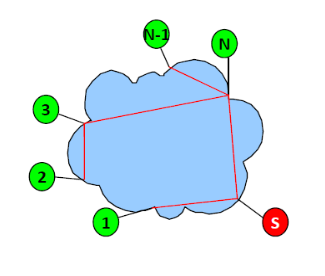
\includegraphics[keepaspectratio]{images/Pasted-image-20260407110113.png}}
Ogni peer che partecipa a una rete P2P deve affrontare quattro problemi
fondamentali: come \textbf{unirsi} alla rete (\emph{join}), come
\textbf{scoprire altri peer} (\emph{peer discovery}), come comportarsi
sia da fornitore che da consumatore di servizi, e come \textbf{prevenire
il free riding} --- ovvero impedire che alcuni nodi consumino risorse
senza contribuire --- incentivando la partecipazione e la reciprocità.

\subsection{Condivisione di Risorse}\label{condivisione-di-risorse}

Le risorse condivise in una rete P2P si trovano ``ai bordi'' di
Internet: sono direttamente messe a disposizione dai peer, senza nodi
speciali per la loro gestione. Possono essere: \textbf{ledger}
distribuiti, spazio di archiviazione in lettura/scrittura, potenza di
calcolo, banda.

La partecipazione può avvenire per motivi molto diversi. Un peer può
offrire risorse gratuitamente per contribuire a un progetto collettivo
(es. ricerca di vita extraterrestre con SETI, ricerca su terapie contro
il cancro). Oppure può essere \textbf{ricompensato} per il contributo
alla gestione della rete, come avviene per i \textbf{Bitcoin miners}. In
ogni caso, la proprietà più interessante è quella di
\textbf{auto-scalabilità}: la partecipazione di un numero crescente di
utenti aumenta naturalmente le risorse del sistema e la sua capacità di
servire più richieste.

\subsection{L'Evoluzione del File
Sharing}\label{levoluzione-del-file-sharing}

Il file sharing è stata la prima \emph{killer application} del P2P. Il
funzionamento tipico è il seguente: un utente U ha un client P2P sul
proprio computer; ad ogni connessione ottiene un nuovo indirizzo IP. U
memorizza i file condivisi in una directory, associando a ciascuno dei
metadati identificativi (titolo, autore, data di pubblicazione). Quando
U vuole trovare un file, invia una query al sistema, riceve la lista dei
peer che lo posseggono, sceglie il peer P secondo certi criteri, e avvia
il trasferimento diretto. Nel frattempo, altri utenti possono già
scaricare da U le parti del file che U ha già ottenuto.

\textbf{Napster} (prima generazione) usava un indice centralizzato dei
file su server dedicati, mentre il trasferimento avveniva direttamente
tra peer. La centralizzazione dell'indice era però un punto di
vulnerabilità --- tecnica e legale --- e portò alla chiusura del
servizio per violazione del copyright: attraverso l'analisi dell'indice
centralizzato era possibile risalire ai contenuti scambiati tra gli
utenti. La seconda generazione (Gnutella, Kazaa, BitTorrent) ha
eliminato ogni punto centrale, distribuendo sia la ricerca che il
trasferimento.

\begin{center}\rule{0.5\linewidth}{0.5pt}\end{center}

\section{Blockchain: Cos'è e Quando
Usarla}\label{blockchain-cosuxe8-e-quando-usarla}

\begin{calloutdefinition}{Blockchain}

Database condiviso, replicato e consistente, mantenuto senza un'autorità
centrale. È \textbf{append-only} (solo aggiunta), immutabile e
resistente alle manomissioni. In termini di teoria dei giochi: una
macchina a stati decentralizzata mantenuta da attori non fidati,
incentivati economicamente a comportarsi correttamente. Non può essere
spenta o censurata, e i dati non possono essere eliminati.

\end{calloutdefinition}

Le tecnologie fondamentali sono: - \textbf{Firme digitali} ---
autenticazione - \textbf{Hash crittografici} --- immutabilità e
integrità - \textbf{Replicazione} --- disponibilità tramite copie
distribuite - \textbf{Consenso distribuito} --- coordinamento tra
repliche mutuamente diffidenti

\begin{callouttip}{Quando usare la blockchain}

Ha senso considerare la blockchain quando: è necessario memorizzare uno
stato condiviso in modalità append-only, ci sono più scrittori con
diversi gradi di fiducia reciproca, l'applicazione deve girare in modo
distribuito, il processo di settlement è complesso e richiede una terza
parte fidata, servono integrità/autenticazione/non-ripudio, le regole
sono precise e semplici da codificare, e la trasparenza è preferibile
alla privacy.

\end{callouttip}

\begin{calloutwarning}{La blockchain non è sempre la soluzione giusta}

Ha senso usarla solo se i partecipanti non sono noti o fidati. Se tutte
le parti sono fidate, un database tradizionale è preferibile. Se serve
solo immutabilità con parti fidate, bastano database con checksum
crittografici (es. AWS QLDB, Kafka). Molti usi proposti della blockchain
in ambito aziendale rientrano in questa categoria e non ne hanno
effettivamente bisogno.

\end{calloutwarning}

\begin{center}\rule{0.5\linewidth}{0.5pt}\end{center}

\section{Bitcoin ed Ethereum}\label{bitcoin-ed-ethereum}

\textbf{Bitcoin} nasce nel 2008 dal paper di Satoshi Nakamoto come
sistema di cassa elettronica P2P: pagamenti online diretti senza
intermediari, con il problema del \textbf{double-spending} risolto
tramite una catena di blocchi con timestamping basato su hash. Il
\emph{Genesis Block} conteneva il messaggio \emph{``Chancellor on brink
of second bailout for banks''} --- un riferimento esplicito alla crisi
finanziaria e all'obiettivo di sottrarre il controllo del denaro alle
banche centrali. La \emph{cypherpunk vision} alla base di Bitcoin è che
si possa rivoluzionare il mondo costruendo protocolli sicuri.

\textbf{Ethereum} espande il concetto: non è solo valuta, ma una
piattaforma programmabile. Introduce gli \textbf{smart contract},
programmi eseguiti dalla blockchain stessa tramite linguaggi
Turing-completi come Solidity. L'intera rete si comporta come un singolo
computer globale replicato e consistente (\textbf{EVM}, Ethereum Virtual
Machine). A differenza di Bitcoin, in cui gli script hanno potere
computazionale limitato, Ethereum può risolvere qualunque problema
computazionale --- con il meccanismo del \textbf{gas} per prevenire
attacchi denial-of-service.

\begin{callouttip}{Smart contract assicurativo}

Un contratto connesso a un database di voli rimborsa automaticamente il
passeggero se il ritardo supera una soglia prestabilita --- senza
pratiche burocratiche, senza intermediari. Il rimborso in criptovaluta
viene trasferito automaticamente al wallet di Bob non appena il ritardo
viene verificato.

\end{callouttip}

\begin{center}\rule{0.5\linewidth}{0.5pt}\end{center}

\section{Le Sfide: Trilemma della
Blockchain}\label{le-sfide-trilemma-della-blockchain}

\begin{calloutwarning}{Trilemma della Blockchain}

È difficile ottenere contemporaneamente \textbf{sicurezza},
\textbf{decentralizzazione} e \textbf{scalabilità}. Migliorare una delle
tre proprietà tende a penalizzare le altre. È una delle grandi sfide
scientifiche aperte del settore.

\end{calloutwarning}

\subsection{Privacy}\label{privacy}

Le transazioni su ledger pubblici sono visibili a tutti. Le identità
degli utenti possono a volte essere inferite, con rischio di esposizione
di dati sensibili. Bilanciare privacy e auditabilità è particolarmente
delicato nei protocolli \textbf{DeFi}: da un lato richiedono
confidenzialità (transazioni, depositi, prestiti senza rivelare importi
o indirizzi), dall'altro richiedono auditabilità (verifica del
double-spending, conferma della collateralizzazione). Le soluzioni
principali sono:

\begin{itemize}
\tightlist
\item
  \textbf{Zero Knowledge Proofs (ZKP)}: un \emph{prover} dimostra la
  validità di un'affermazione a un \emph{verifier} senza rivelare i dati
  sottostanti. Applicazioni: nascondere dati sensibili mantenendo la
  correttezza, esecuzione privata di smart contract, verifica d'identità
  privata on-chain, DeFi privacy-preserving.
\item
  \textbf{Fully Homomorphic Encryption (FHE)}: eseguire calcoli su dati
  cifrati senza decifrarli --- il risultato, una volta decifrato,
  coincide con quello ottenuto dal testo in chiaro. L'idea chiave è:
  \emph{``posso calcolare sui tuoi dati segreti senza mai vederli''}.
  Esempio: un protocollo di prestito calcola l'idoneità al credito o il
  tasso di interesse su saldi cifrati --- i saldi restano privati ma il
  sistema produce risultati corretti.
\item
  \textbf{Multiparty Computation (MPC)}: calcolo distribuito tra più
  parti che collaborano senza rivelare i propri input privati alle
  altre.
\end{itemize}

\subsection{Scalabilità}\label{scalabilituxe0}

Le blockchain tradizionali hanno throughput limitato e costi energetici
elevati. Le soluzioni principali spostano l'esecuzione
\textbf{off-chain}, usando la catena principale solo come ancora di
fiducia (\emph{trust anchor}) per la validazione finale:

\begin{itemize}
\tightlist
\item
  \textbf{Layer-2} (Optimistic Rollups, ZK-rollups): raggruppano molte
  transazioni off-chain e ne pubblicano solo la prova sulla catena
  principale.
\item
  \textbf{Payment Channel} (Lightning Network): canali di pagamento
  bidirezionali che consentono scambi diretti tra peer senza toccare la
  blockchain per ogni transazione.
\end{itemize}

\begin{center}\rule{0.5\linewidth}{0.5pt}\end{center}

\section{Applicazioni}\label{applicazioni}

{\def\LTcaptype{none} % do not increment counter
\begin{longtable}[]{@{}
  >{\raggedright\arraybackslash}p{(\linewidth - 2\tabcolsep) * \real{0.5000}}
  >{\raggedright\arraybackslash}p{(\linewidth - 2\tabcolsep) * \real{0.5000}}@{}}
\toprule\noalign{}
\begin{minipage}[b]{\linewidth}\raggedright
Applicazione
\end{minipage} & \begin{minipage}[b]{\linewidth}\raggedright
Descrizione
\end{minipage} \\
\midrule\noalign{}
\endhead
\bottomrule\noalign{}
\endlastfoot
\textbf{Criptovalute e Token} & Alternativa alle valute fiat: la
blockchain non richiede che un governo emetta moneta né che le banche
validino le transazioni. L'offerta è legata a un bene virtuale limitato
crittograficamente. La blockchain risolve il double spending e supporta
sia token \textbf{fungibili} (interscambiabili) che \textbf{non
fungibili} \\
\textbf{NFT} & Prova di proprietà di asset digitali unici (arte, diritti
d'autore). Un'opera in .jpeg è facilmente copiabile, ma l'NFT certifica
chi è il proprietario originale \\
\textbf{DeFi} & Piattaforme come \textbf{Uniswap} per il trading diretto
tra pari (DEX) con pool di liquidità e market maker automatizzati (AMM).
In Uniswap V3, le posizioni di liquidità sono rappresentate come
\textbf{LP NFTs}: ogni posizione ha parametri distinti e
personalizzabili che ne determinano valore e rendimento \\
\textbf{Self Sovereign Identity} & L'utente controlla i propri dati e
rivela solo le informazioni minime necessarie (minimalismo, portabilità,
consenso) \\
\textbf{Supply Chain} & Tracciamento provenienza e qualità: es.
Walmart-IBM (Hyperledger) per sicurezza alimentare, con sensori IoT che
registrano temperatura e posizione. Un altro esempio: ristoranti possono
verificare la catena di custodia del pesce, con sensori attaccati al
prodotto che registrano posizione, temperatura e umidità lungo tutta la
filiera \\
\textbf{Intellectual Property} & Il proprietario di un contenuto
digitale fa l'hash del contenuto insieme alla propria identità e lo
registra sulla blockchain. Se nessun altro può dimostrare di averlo
pubblicato prima di quel commit, questo costituisce prova di proprietà
--- più comodo di un ufficio brevetti e senza dover divulgare i dettagli
del contenuto \\
\end{longtable}
}

\begin{center}\rule{0.5\linewidth}{0.5pt}\end{center}

\section{Conclusioni e Prospettive}\label{conclusioni-e-prospettive}

I sistemi P2P offrono vantaggi su più fronti. Per gli utenti:
sfruttamento delle risorse in eccesso (cicli CPU inutilizzati, storage
libero, banda disponibile) in cambio di risorse, servizi o
partecipazione a reti sociali. Per la comunità: la \textbf{proprietà di
auto-scalabilità} --- la partecipazione di un numero maggiore di utenti
aumenta naturalmente le risorse del sistema. Per chi sviluppa
applicazioni: riduzione dei costi rispetto al modello client-server
(server farm ad alta connettività, replicazione per fault tolerance,
disponibilità 24×7 sono tutte responsabilità distribuite tra i peer).

Il successo di un'applicazione P2P dipende in larga misura dalla
formazione di una \textbf{massa critica} di utenti: una soglia di
partecipazione che permette all'applicazione di autosostenersi. Nei
primi sistemi P2P questa soglia è stata raggiunta grazie alla novità
dell'applicazione (contenuti gratuiti nel file sharing, criptovalute
come asset redditizio, token come mezzo semplice per scambiare asset).
Per le nuove applicazioni, il successo dipenderà oltre che dalla qualità
tecnica anche dall'\textbf{appeal dell'applicazione} e dalla definizione
di nuovi \textbf{modelli di business}.

\begin{calloutnote}{Sfide scientifiche aperte}

Lo sviluppo di applicazioni P2P su larga scala richiede strumenti nuovi.
Le metodologie classiche per i sistemi distribuiti non scalano: un
sistema P2P opera su milioni di nodi (non centinaia), e il fallimento o
la disconnessione di un nodo è un evento normale, non un'eccezione.
Servono: \textbf{teoria dei giochi} (cooperazione tra peer, equilibrio
di Nash), \textbf{nuove tecniche crittografiche}, \textbf{nuovi
algoritmi di consenso}, \textbf{strumenti di analisi di sistemi
complessi}.

\end{calloutnote}

\newpage

\chapter{Classificazione degli Overlay: Overlay Non
Strutturati}\label{classificazione-degli-overlay-overlay-non-strutturati}

\section{Dal Centralizzato al P2P}\label{dal-centralizzato-al-p2p}

Napster (2001) ha dimostrato che si può servire una quantità di dati
paragonabile a Google con molti meno server, spostando storage e
trasferimento direttamente sugli utenti. All'epoca Google impiegava
circa 15.000 server, Napster circa 100. Il sistema raggiunge 26,4
milioni di utenti nel 2001, con 10 TB di dati (2 milioni di canzoni, in
media 220 per utente). I server si occupano solo di localizzare chi
possiede la risorsa --- la parte meno costosa del servizio. In questo
modello ogni utente è un \textbf{servent} (server + client): partecipa
``pagando'' con le proprie risorse fisiche, contenuti o conoscenza.

\textbf{Punti di forza di Napster}: sistema informativo globale senza
grandi investimenti, decentralizzazione dei costi e
dell'amministrazione, nessun collo di bottiglia sulle risorse (storage e
trasferimento distribuiti tra gli utenti). \textbf{Punti di debolezza}:
il server resta un singolo punto di fallimento e di controllo,
necessario per gestire l'intero sistema --- esattamente questo lo ha
reso vulnerabile agli attacchi legali per violazione del copyright,
poiché l'analisi dell'indice centralizzato permetteva di risalire ai
contenuti scambiati.

\textbf{Gnutella} rimuove anche quest'ultimo punto centrale: nessun
indice, connessioni dirette tra peer usate per la ricerca (non per il
download). Il risultato è un sistema senza infrastruttura né
amministrazione, privo di single point of failure. I punti deboli
diventano: alto traffico di rete, assenza di ricerca strutturata, e
\textbf{free riding} (nodi che consumano risorse senza contribuire).

\begin{center}\rule{0.5\linewidth}{0.5pt}\end{center}

\section{Reti Overlay}\label{reti-overlay}

\begin{calloutdefinition}{Overlay Network}

Rete logica costruita sopra la rete fisica sottostante (underlay),
tipicamente a livello applicativo sopra TCP/IP. I link dell'overlay sono
``tunnel'' che attraversano la rete fisica: un singolo collegamento
logico può passare per decine di router. Più overlay possono coesistere
contemporaneamente sulla stessa rete fisica, ciascuno offrendo il
proprio servizio specifico non disponibile nell'underlay. I nodi
dell'overlay sono spesso end host che fungono anche da nodi intermedi
che inoltrano traffico.

\end{calloutdefinition}

\pandocbounded{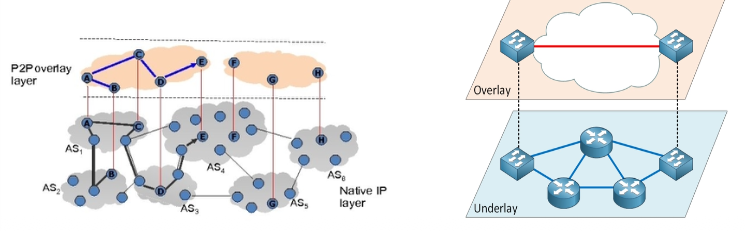
\includegraphics[keepaspectratio]{images/Pasted-image-20260407110328.png}}
Un protocollo P2P definisce formato e semantica dei messaggi tra peer. I
peer sono identificati da ID univoci, generalmente calcolati tramite
funzioni hash. I pacchetti P2P, analogamente ai pacchetti IP, sono
caratterizzati da un \textbf{header} e un \textbf{payload}. Il
protocollo definisce anche una strategia di routing a livello
applicativo dello stack TCP/IP, senza dover modificare i router
sottostanti.

\section{Classificazione degli
Overlay}\label{classificazione-degli-overlay}

{\def\LTcaptype{none} % do not increment counter
\begin{longtable}[]{@{}
  >{\raggedright\arraybackslash}p{(\linewidth - 6\tabcolsep) * \real{0.2500}}
  >{\raggedright\arraybackslash}p{(\linewidth - 6\tabcolsep) * \real{0.2500}}
  >{\raggedright\arraybackslash}p{(\linewidth - 6\tabcolsep) * \real{0.2500}}
  >{\raggedright\arraybackslash}p{(\linewidth - 6\tabcolsep) * \real{0.2500}}@{}}
\toprule\noalign{}
\begin{minipage}[b]{\linewidth}\raggedright
Tipo
\end{minipage} & \begin{minipage}[b]{\linewidth}\raggedright
Topologia
\end{minipage} & \begin{minipage}[b]{\linewidth}\raggedright
Lookup
\end{minipage} & \begin{minipage}[b]{\linewidth}\raggedright
Garanzie
\end{minipage} \\
\midrule\noalign{}
\endhead
\bottomrule\noalign{}
\endlastfoot
\textbf{Centralizzato} & Server centrale & \(O(1)\) & Singolo punto di
fallimento \\
\textbf{Non Strutturato} & Grafo casuale & \(O(N)\) & Nessuna garanzia
di trovare la risorsa \\
\textbf{SuperPeer (Ibrido)} & Gerarchico & \(O(hops_{max})\) & Migliore
scalabilità del non strutturato \\
\textbf{Strutturato (DHT)} & Topologia controllata & \(O(\log N)\) &
Lookup garantito, garanzie anche su join e leave \\
\end{longtable}
}

\begin{center}\rule{0.5\linewidth}{0.5pt}\end{center}

\section{Overlay Non Strutturati}\label{overlay-non-strutturati}

I peer si connettono arbitrariamente: la topologia forma un grafo
casuale (es. Gnutella ≤ 0.4, Bitcoin). La rete è resiliente e facile da
mantenere, ma la ricerca è costosa --- nel caso peggiore \(O(N)\). I
falsi negativi sono possibili: la risorsa cercata potrebbe esistere ma
non essere raggiunta entro il TTL.

\subsection{Bootstrapping e Discovery}\label{bootstrapping-e-discovery}

Un nuovo nodo non conosce nessuno. Il \textbf{bootstrapping} avviene
tramite due meccanismi complementari: server DNS noti che memorizzano
gli indirizzi IP di un insieme di peer stabili (eseguendo script che
interagiscono con i peer e aggiornano automaticamente la lista), oppure
una \textbf{cache interna} in cui ogni client memorizza gli IP dei peer
contattati nelle sessioni correnti e precedenti, aggiornata
dinamicamente tramite \emph{gossiping} con i vicini.
\pandocbounded{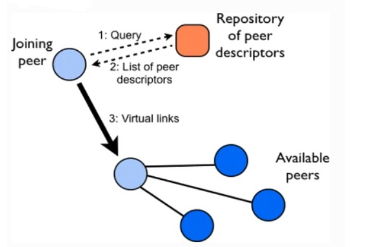
\includegraphics[keepaspectratio]{images/Pasted-image-20260407110433.png}}
Il processo di partecipazione alla rete si articola in tre fasi:

\begin{itemize}
\tightlist
\item
  \textbf{Step 0} --- join: il nodo si connette a uno o più peer noti
  tramite bootstrap.
\item
  \textbf{Step 1} --- peer discovery: il nodo invia messaggi
  \textbf{Ping} per annunciare la propria presenza; i peer rispondono
  con \textbf{Pong} contenenti le proprie informazioni e inoltrano il
  Ping ai vicini.
\item
  \textbf{Step 2} --- searching: il nodo invia una query ai vicini (es.
  \emph{``do you have any content that matches the string `Back to
  Black'?''}); i peer che hanno corrispondenze rispondono, gli altri
  inoltrano la query per TTL salti.
\item
  \textbf{Step 3} --- downloading: il trasferimento avviene via
  connessioni HTTP dirette usando il metodo GET.
\end{itemize}

\subsection{Flooding}\label{flooding}

L'algoritmo di ricerca base è il \textbf{Flooding}: la query viene
inviata a tutti i vicini, che la inoltrano a loro volta. Per evitare
loop infiniti si usa un \textbf{TTL} decrementato ad ogni salto; quando
raggiunge zero il messaggio viene scartato. I duplicati si evitano con
un ID univoco per ogni messaggio. Le risposte viaggiano all'indietro
attraverso le connessioni non transitorie, tramite \textbf{Backward
Routing}.

\begin{verbatim}
FloodForward(Query q, Source p):
  if q.id ∈ oldIdsQ: return          // duplicato, scarta
  oldIdsQ ← oldIdsQ ∪ {q.id}
  q.TTL ← q.TTL - 1
  if q.TTL == 0: return              // scaduto, scarta
  foreach s ∈ Neighbors:
    if s ≠ p: send(s, q)             // inoltra a tutti tranne il mittente
\end{verbatim}

Il flooding equivale a una \textbf{BFS limitata dal TTL}: trova il
massimo numero di risultati nel raggio TTL centrato sul nodo sorgente.
Garantisce alta resilienza ma genera molto traffico e molti duplicati,
scala male, e \textbf{non garantisce il ritrovamento della risorsa}
(false negative). È usato anche in \textbf{Bitcoin} non solo per la
ricerca, ma per \textbf{propagare le transazioni} nella rete P2P
sottostante --- dove mantenere la consistenza è la sfida principale.

\subsection{Tecniche di Ricerca
Avanzate}\label{tecniche-di-ricerca-avanzate}

Le alternative al flooding puro si dividono in due categorie: approcci
\textbf{BFS-based} (iterative deepening/expanding ring, k-walker random
walk, two-level k-walker, directed BFS, modified random BFS) e approcci
\textbf{DFS-based} (local indices, routing indices, attenuated bloom
filter).

\textbf{Expanding Ring (Iterative Deepening)} --- BFS con TTL crescente.
Si parte da un TTL basso (opzionalmente su un sottoinsieme casuale dei
vicini); se la ricerca fallisce si ripete incrementandolo fino alla
terminazione (risorsa trovata o profondità massima raggiunta). Per non
riprocessare gli stessi nodi, quelli al bordo dell'anello \emph{i-esimo}
\textbf{congelano} la query per un periodo \(> W\) (intervallo tra due
query successive). Quando la sorgente invia un messaggio \texttt{resend}
con lo stesso ID e un \texttt{NewTTL} maggiore, i nodi interni
all'anello precedente lo inoltrano semplicemente; i nodi al bordo lo
\textbf{scongelano} e inviano la query ai propri vicini con
\(TTL = NewTTL - PreviousTTL\).

\textbf{Random Walk e k-Walker} --- Il random walk è modellato come una
\textbf{catena di Markov} (\emph{drunkard's walk}): il sistema è privo
di memoria, la distribuzione di probabilità dello stato futuro dipende
solo dallo stato presente, senza direzioni privilegiate. In pratica, il
nodo invia la query a \emph{un solo} vicino scelto a caso, che fa lo
stesso; il TTL si decrementa ad ogni salto. Se la ricerca fallisce
(timeout), la sorgente può riemettere la query lungo un altro cammino
casuale. Riduce drasticamente il traffico ma aumenta la latenza.

La variante \textbf{k-walker} parallelizza inviando \(k\) copie
indipendenti, ciascuna che prende il proprio cammino casuale. La
terminazione può avvenire per TTL oppure con un \textbf{checking
method}: i walker periodicamente verificano con la sorgente se la
condizione di stop è stata soddisfatta. Si può anche \textbf{bilanciare
verso nodi ad alto grado} modulando la probabilità di scelta del vicino.
Vantaggi e svantaggi: il limite superiore al traffico è \(k \times TTL\)
messaggi; \(k\) walker dopo \(T\) passi raggiungono circa lo stesso
numero di nodi di 1 walker dopo \(k \times T\) passi, riducendo il
ritardo di un fattore \(k\). Le prestazioni dipendono da \(k\), \(T\) e
dalla popolarità \(p\) della risorsa: \(k\) e \(T\) bassi producono alto
ritardo e bassa probabilità di successo; \(k\) e \(T\) alti producono
alto overhead. Una soluzione è impostare i parametri adattativamente in
funzione della popolarità.

\textbf{Directed BFS e Routing Indices} --- I vicini vengono scelti non
a caso ma selezionando i ``migliori''. Un vicino è considerato buono se:
ha prodotto risultati in passato, ha bassa latenza, ha il minor numero
di hop per i risultati (segno che ha buoni vicini), ed è stabile. Dopo
il primo hop, la ricerca può proseguire come un normale BFS.

I \textbf{Routing Indices (RI)} formalizzano questa selezione: ogni peer
mantiene una struttura dati che, data una query, restituisce la lista
dei vicini ordinata per ``bontà''. Ogni peer ha un indice locale per i
propri documenti e un RI che stima quanti documenti sono disponibili per
ciascun percorso e per ciascun argomento. Esempio: per il nodo A,
tramite il vicino B e i suoi discendenti sono disponibili 100 documenti
--- 20 nella categoria Database, 10 in Theory, 30 in Languages. Questo
permette di inviare la query solo ai vicini più rilevanti per quella
specifica ricerca.

\begin{center}\rule{0.5\linewidth}{0.5pt}\end{center}

\section{Overlay Strutturati (DHT)}\label{overlay-strutturati-dht}

Negli overlay \textbf{strutturati} la scelta dei vicini segue criteri
precisi, generando una topologia controllata. L'obiettivo è garantire
scalabilità: il lookup è \textbf{key-based} con complessità
\(O(\log N)\), e le garanzie valgono anche per le operazioni di join e
leave dei peer. Esempi: \textbf{CAN}, \textbf{Chord}, \textbf{Pastry},
\textbf{Kademlia}.

\begin{center}\rule{0.5\linewidth}{0.5pt}\end{center}

\section{Overlay Ibridi (SuperPeer)}\label{overlay-ibridi-superpeer}

\begin{calloutdefinition}{SuperPeer}

Nodo con maggiore capacità (banda, CPU, disponibilità) che funge da hub
locale. I peer normali si connettono ai SuperPeer e depositano l'indice
delle proprie risorse. Il flooding per la ricerca avviene solo tra
SuperPeer; il trasferimento dei file resta diretto tra peer.

\end{calloutdefinition}

I SuperPeer vengono scelti autonomamente dal sistema in base alle
capacità (storage, banda) e alla disponibilità (tempo di connessione),
definendo dinamicamente un livello gerarchico nella rete. Periodicamente
si scambiano informazioni sulle risorse dei peer collegati e si fanno
carico del carico dei nodi più lenti. I peer ordinari caricano la
descrizione delle proprie risorse sul SuperPeer, lo interrogano per le
query, e partecipano direttamente al trasferimento delle risorse.

Il vantaggio è che il traffico di ricerca è contenuto alla rete dei
SuperPeer, migliorando la scalabilità rispetto al non strutturato puro
--- a scapito di una minore resistenza al churn dei SuperPeer stessi.

\begin{calloutnote}{Differenza tra implementazioni}

In \textbf{Gnutella v0.6} gli \emph{ultrapeers} sono
\textbf{auto-promossi} dai nodi stessi in base alle proprie capacità. In
\textbf{Kazaa}, \textbf{Skype} (per il relay) e \textbf{eDonkey}
(pre-Kad) gli ultrapeers sono invece \textbf{staticamente definiti}.

\end{calloutnote}

\begin{center}\rule{0.5\linewidth}{0.5pt}\end{center}

\section{Auto-Organizzazione}\label{auto-organizzazione}

Le reti non strutturate mostrano proprietà emergenti simili a fenomeni
fisici e biologici: dall'interazione locale dei peer emerge
spontaneamente una struttura globale, senza alcun coordinamento
centrale. In fisica, il \textbf{fenomeno di Bénard} mostra come una
sostanza magnetica riscaldata da un lato e raffreddata dall'altro formi
spontaneamente strutture regolari. In biologia, le colonie di insetti
come le termiti producono strutture complesse senza alcun coordinamento
centrale. In Gnutella emerge spontaneamente un \textbf{backbone} --- una
rete di nodi con alto grado di connessione (simili a server) che
organizzano il traffico della rete, senza che nessuno lo abbia
pianificato.

\newpage

\chapter{Introduzione alle DHT: Consistent Hashing e
Routing}\label{introduzione-alle-dht-consistent-hashing-e-routing}

\section{Il Problema del Recupero
Distribuito}\label{il-problema-del-recupero-distribuito}

In una rete P2P pura il problema fondamentale è il seguente: il nodo A
possiede un contenuto I, il nodo B lo vuole ma non ne conosce la
posizione. Come decidere dove memorizzare I e come trovarlo, senza
ricorrere a un server centralizzato? Qualsiasi soluzione deve fare i
conti con due requisiti irrinunciabili: la \textbf{scalabilità} ---
l'overhead di comunicazione e la memoria richiesta da ogni nodo devono
essere funzioni contenute del numero di peer N --- e
l'\textbf{adattabilità}, ovvero la capacità di reggere ai guasti e al
\emph{churn} continuo di nodi che si connettono e disconnettono.

\begin{center}\rule{0.5\linewidth}{0.5pt}\end{center}

\section{Searching vs Addressing}\label{searching-vs-addressing}

In un sistema P2P puro, il recupero dei contenuti può seguire due
paradigmi opposti.

Il \textbf{searching} guida la ricerca attraverso gli attributi del
contenuto, in modo analogo a un motore di ricerca. Il vantaggio è
l'immediatezza per l'utente: non sono necessarie strutture ausiliarie e
le query complesse sono ammesse. Lo svantaggio è la scalabilità: nelle
reti non strutturate con flooding ogni nodo contatta tutti i propri
vicini, portando a un overhead di comunicazione \(O(N^2)\) nel caso
peggiore. Con ottimizzazioni come TTL e identificatori per evitare cicli
il costo scende a \(O(N)\), ma rimane comunque proibitivo per reti
grandi.

L'\textbf{addressing} assegna un identificatore univoco a ogni contenuto
--- tipicamente il suo hash crittografico --- e usa quella chiave per
recuperarlo. È il fondamento delle \textbf{Distributed Hash Tables
(DHT)}: l'hash del contenuto diventa la chiave di accesso, e la DHT
instrada la query verso il nodo responsabile di quella chiave con
garanzie teoriche precise. Il compromesso è la rinuncia alle query
complesse e il costo del mantenimento della struttura di indirizzamento.
Questo approccio non è più \emph{location-based} (URL che puntano a una
posizione), ma \emph{content-based} (l'identità del dato è il suo hash,
come fa IPFS).

\begin{center}\rule{0.5\linewidth}{0.5pt}\end{center}

\section{Motivazione per le DHT}\label{motivazione-per-le-dht}

Il punto di partenza è confrontare i due estremi già noti.

L'\textbf{approccio centralizzato} (un server di indicizzazione) offre
ricerca in \(O(1)\) e query complesse senza sforzo, ma richiede spazio
\(O(N)\) e banda \(O(N)\) sul server, ed è un single point of failure.
L'\textbf{approccio completamente distribuito} (rete non strutturata con
flooding) non richiede strutture dati per il routing (\(O(1)\) memoria
per nodo) ed è intrinsecamente robusto, ma il costo di ricerca esplode a
\(O(N^2)\), con falsi negativi in caso di partizionamento.

Le DHT si collocano nel punto ottimale di compromesso tra i due:

\pandocbounded{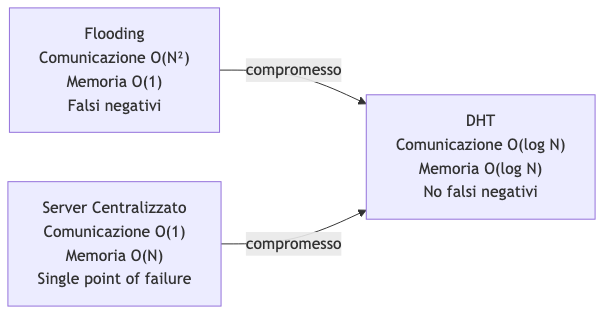
\includegraphics[keepaspectratio,alt={Diagramma Mermaid}]{images/mermaid-lezione-3-retrieving-content-e-dht-01.png}}
\emph{Fig. --- Le DHT si collocano nel punto di compromesso:
\(O(\log N)\) sia per la comunicazione che per la memoria, senza falsi
negativi e con auto-organizzazione.}

Le proprietà chiave che la DHT garantisce rispetto al flooding sono:
scalabilità \(O(\log N)\), assenza di falsi negativi, e
\emph{self-organization} --- il sistema gestisce autonomamente join e
leave dei nodi, sia volontari che per guasto.

\begin{center}\rule{0.5\linewidth}{0.5pt}\end{center}

\section{Funzioni Hash}\label{funzioni-hash}

Una \textbf{funzione hash} mappa dati di lunghezza arbitraria in un
valore di lunghezza fissa (tipicamente un intero). Poiché l'insieme
degli input è più grande dell'insieme degli output, le
\textbf{collisioni} sono inevitabili. In una \textbf{hash table}
classica, la chiave viene hashata per trovare direttamente il bucket, e
ogni bucket contiene in media
\(\frac{\text{\#items}}{\text{\#buckets}}\) elementi.

Le \textbf{funzioni hash crittografiche} devono soddisfare proprietà
aggiuntive di sicurezza rispetto alle semplici hash table. Il caso d'uso
principale è \textbf{SHA} (Secure Hash Algorithm), la famiglia di
standard usata anche nelle DHT:

\begin{itemize}
\tightlist
\item
  Input di lunghezza variabile → output di lunghezza fissa
  (\emph{digest})
\item
  Una piccola variazione nell'input produce output completamente diversi
  (\emph{effetto valanga})
\item
  La funzione è deterministica: lo stesso input produce sempre lo stesso
  output
\item
  SHA-1 produce un digest di 40 cifre esadecimali = 160 bit →
  \(2^{160}\) valori possibili
\end{itemize}

\begin{callouttip}{Output SHA-1 in Java}

\begin{verbatim}
SHA1("")    = DA39A3EE5E6B4B0D3255BFEF95601890AFD80709
SHA1("abc") = A9993E364706816ABA3E25717850C26C9CD0D89D
SHA1("abd") = CB4CC28DF0FDBE0ECF9D9662E294B118092A5735
\end{verbatim}

``abc'' e ``abd'' differiscono di un solo carattere ma producono digest
completamente diversi --- l'effetto valanga in azione. La stringa vuota
produce un digest ben definito, non un errore.

\end{callouttip}

Le famiglie disponibili sono SHA-1, SHA-224, SHA-256, SHA-384 e SHA-512,
dove le ultime quattro sono note come \textbf{SHA-2} e il suffisso
indica la lunghezza in bit del digest. Ethereum usa \textbf{Keccak} (una
variante di SHA-3). Queste funzioni sono il mattone base sia per il
consistent hashing delle DHT sia per i puzzle crittografici del Proof of
Work di Bitcoin.

\begin{center}\rule{0.5\linewidth}{0.5pt}\end{center}

\section{Da Memcached alle DHT}\label{da-memcached-alle-dht}

\textbf{Memcached} è un sistema di caching distribuito per il web:
mantiene un pool di server che forniscono accesso rapido alle
informazioni, riducendo il carico sul database (l'accesso al DB avviene
solo in caso di \emph{cache miss}). L'idea è distribuire una hash table
su più server per superare i limiti di memoria di una singola macchina.

Il meccanismo di base: l'hash dell'URL di una risorsa determina in quale
server di cache è memorizzata; ogni macchina può calcolare
\emph{localmente} quale cache contiene la risorsa cercata, senza
comunicazione tra le cache stesse. Questo schema viene esteso alle DHT
per i sistemi P2P --- ma in uno scenario dinamico emerge immediatamente
il \textbf{problema del rehashing}.

\begin{center}\rule{0.5\linewidth}{0.5pt}\end{center}

\section{Il Problema del Rehashing}\label{il-problema-del-rehashing}

Le hash table distribuite classiche calcolano il nodo target come
\(h(\text{key}) \bmod N\), dove \(N\) è il numero di server. Con \(N\)
fisso tutto funziona: 4 bucket con 12 chiavi assegnate uniformemente, ad
esempio:

{\def\LTcaptype{none} % do not increment counter
\begin{longtable}[]{@{}ll@{}}
\toprule\noalign{}
Bucket & Chiavi assegnate \\
\midrule\noalign{}
\endhead
\bottomrule\noalign{}
\endlastfoot
1 & 1, 5, 9 \\
2 & 2, 6, 10 \\
3 & 3, 7, 11 \\
4 & 4, 8, 12 \\
\end{longtable}
}

Ora supponiamo che il bucket 3 vada offline e si aggiunga un nuovo
bucket 5. Con \(N\) che cambia da 4 a 4 (dopo la rimozione), il calcolo
\(h(\text{key}) \bmod 4\) rimane valido solo per le chiavi già
allineate. Con il nuovo bucket 5 e \(N=4 \to N=4\) la situazione è
ancora peggio: le chiavi che restano sullo stesso nodo sono solo quelle
per cui \(h(\text{key}) \bmod 4 = h(\text{key}) \bmod 5\), che è una
piccola minoranza.

\begin{calloutwarning}{Entità del problema}

Con la funzione classica \(\text{SHA}(x) \bmod N\): - 4 nodi di caching
→ 6 nodi: quasi tutte le chiavi devono essere rimappate - Con 10 bucket
e 1000 chiavi, circa il \textbf{99\% delle chiavi deve essere
riassegnato} - Questo produce un traffico enorme che satura la rete,
rendendo il sistema inutilizzabile durante ogni operazione di scaling

\end{calloutwarning}

Il problema è aggravato dal fatto che le chiavi vengono rimappate anche
sui nodi che sono rimasti attivi --- non solo a causa delle aggiunte o
rimozioni, ma per il semplice cambiamento di \(N\). In un sistema P2P
con churn continuo, questo è inaccettabile.

\begin{center}\rule{0.5\linewidth}{0.5pt}\end{center}

\section{Consistent Hashing}\label{consistent-hashing}

\begin{calloutdefinition}{Consistent Hashing}

Tecnica di hashing in cui sia i contenuti che i nodi vengono mappati
nello \textbf{stesso spazio di indirizzamento}, organizzato come un
\textbf{anello circolare} (\emph{ring}) di dimensione \(2^M\). Ogni nodo
gestisce un \textbf{intervallo contiguo} di chiavi dell'anello, non un
insieme sparso come avviene con il modulo. Lo schema non dipende
direttamente dal numero di server: aggiungere o rimuovere nodi richiede
di spostare solo una minoranza di elementi --- in media \(K/n\) chiavi,
dove \(K\) è il totale delle chiavi e \(n\) il numero di nodi.

\end{calloutdefinition}

L'intuizione fondamentale è semplice: invece di mappare gli oggetti a un
\emph{indice di bucket} che dipende da \(N\), si mappano sia gli oggetti
che i nodi nello stesso spazio continuo, e si assegna ogni oggetto al
primo nodo che si incontra procedendo in senso orario. Così, quando
\(N\) cambia, solo i nodi adiacenti alla modifica sono coinvolti nella
redistribuzione.

\begin{center}\rule{0.5\linewidth}{0.5pt}\end{center}

\section{Costruzione di una DHT:
l'Anello}\label{costruzione-di-una-dht-lanello}

La costruzione di una DHT basata su consistent hashing segue tre passi
concettuali.

\textbf{Passo 1 --- Spazio di chiavi comune.} Si definisce un
\emph{identifier space} condiviso tra nodi e dati, tipicamente
\(\{0, 1, \ldots, 2^M - 1\}\) organizzato come un anello modulo \(2^M\).
Tutti gli identificatori --- sia dei nodi che dei contenuti --- vivono
in questo spazio.

\textbf{Passo 2 --- Connessione dei nodi.} Ogni nodo è collegato a un
numero piccolo e limitato di vicini in modo tale che il numero massimo
di hop sia limitato. La topologia dell'overlay definisce diverse
strutture possibili: anello con \emph{chord} (scorciatoie), albero, ecc.

\textbf{Passo 3 --- Assegnazione dei dati.} Sia i nodi che i dati
vengono mappati dalla stessa funzione hash nello stesso spazio; si
definisce una relazione tra hash dei contenuti e hash dei nodi per
determinare chi memorizza cosa.

\subsection{Costruzione dell'Anello: Esempio con
N=16}\label{costruzione-dellanello-esempio-con-n16}

Consideriamo uno spazio di identificatori \(\{0, \ldots, 15\}\)
organizzato come un anello modulo 16, con cinque nodi \(a, b, c, d, e\)
che ottengono le seguenti posizioni tramite la funzione hash \(H\):

\[H(a) = 6, \quad H(b) = 5, \quad H(c) = 0, \quad H(d) = 11, \quad H(e) = 2\]

\pandocbounded{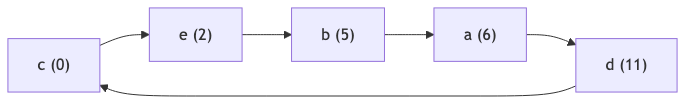
\includegraphics[keepaspectratio,alt={Diagramma Mermaid}]{images/mermaid-lezione-3-retrieving-content-e-dht-02.png}}
\emph{Fig. --- Anello con N=16 e cinque nodi. I nodi (cerchi verdi) sono
posizionati alle posizioni 0, 2, 5, 6, 11 dell'anello; ogni nodo punta
al proprio successore, formando una lista circolare.}

\subsection{Il Successore}\label{il-successore}

Il \textbf{successore} \texttt{succ(x)} è il primo nodo sull'anello con
identificatore \(\geq x\), procedendo in senso orario. Importanti
distinzioni: \texttt{succ} può essere applicato sia a identificatori
generici (non occupati da nodi) sia a posizioni di nodi.

\begin{callouttip}{Calcolo del successore}

\begin{itemize}
\tightlist
\item
  \texttt{succ(12)\ =\ 0} --- non ci sono nodi tra 12 e 15, si fa
  wrap-around all'inizio dell'anello
\item
  \texttt{succ(1)\ =\ 2} --- il nodo più vicino in senso orario a
  partire da 1 è il nodo in posizione 2
\item
  \texttt{succ(6)\ =\ 6} --- la posizione 6 è occupata da un nodo,
  quindi il successore coincide
\end{itemize}

È fondamentale distinguere tra gli \textbf{identificatori} (tutti i
valori 0--15) e i \textbf{nodi} (solo le cinque posizioni occupate).

\end{callouttip}

Il successore di un nodo \(n\) è definito come \texttt{succ(n+1)}: - Il
successore di 0 è \texttt{succ(1)\ =\ 2} - Il successore di 2 è
\texttt{succ(3)\ =\ 5} - Il successore di 5 è \texttt{succ(6)\ =\ 6} -
Il successore di 6 è \texttt{succ(7)\ =\ 11} - Il successore di 11 è
\texttt{succ(12)\ =\ 0} (wrap-around)

\subsection{Dove Memorizzare i Dati}\label{dove-memorizzare-i-dati}

I dati vengono memorizzati usando la stessa funzione hash \(H\)
applicata alla chiave del contenuto. Una coppia
\texttt{\textless{}key,\ value\textgreater{}} --- ad esempio
\texttt{key="crown"}, \texttt{value=JPEG\ della\ corona} --- ottiene un
identificatore \(k = H(\text{key})\), e il dato viene archiviato nel
nodo \texttt{succ(k)}.

Nell'esempio, i dati del gioco vengono distribuiti sull'anello così:

{\def\LTcaptype{none} % do not increment counter
\begin{longtable}[]{@{}lll@{}}
\toprule\noalign{}
Oggetto & Hash & Nodo responsabile (\texttt{succ}) \\
\midrule\noalign{}
\endhead
\bottomrule\noalign{}
\endlastfoot
Scudo & \(H(\text{scudo}) = 12\) & \texttt{succ(12)\ =\ 0} \\
Ascia & \(H(\text{ascia}) = 2\) & \texttt{succ(2)\ =\ 2} \\
Corona & \(H(\text{corona}) = 9\) & \texttt{succ(9)\ =\ 11} \\
Spada & \(H(\text{spada}) = 14\) & \texttt{succ(14)\ =\ 0} \\
Anello & \(H(\text{anello}) = 4\) & \texttt{succ(4)\ =\ 5} \\
\end{longtable}
}

Ogni oggetto si ``sposta'' in senso orario fino al primo nodo che
incontra. Lo scudo (hash=12) e la spada (hash=14) atterrano entrambi sul
nodo 0 perché non ci sono nodi tra 12 e 15.

\subsection{Peer Leave: Consistent Hashing in
Azione}\label{peer-leave-consistent-hashing-in-azione}

\begin{callouttip}{Rimozione del nodo 11}

Se il nodo 11 abbandona la rete, solo le chiavi che gli erano assegnate
devono essere rimappate --- e vengono assegnate al suo successore, il
nodo 0. La corona (hash=9) passa da nodo 11 a nodo 0. Tutti gli altri
oggetti (ascia su nodo 2, anello su nodo 5, scudo e spada su nodo 0)
restano invariati. Il resto dell'anello non è toccato dalla rimozione.

\end{callouttip}

Questa è la proprietà chiave del consistent hashing: modificare di
un'unità il numero di nodi non forza il rimapping globale, ma solo
locale.

\begin{center}\rule{0.5\linewidth}{0.5pt}\end{center}

\section{Proprietà del Consistent
Hashing}\label{proprietuxe0-del-consistent-hashing}

Quando la hash table viene ridimensionata, in media solo \(K/n\) chiavi
devono essere rimappate (dove \(K\) è il numero totale di chiavi, \(n\)
il numero di server), a patto che la funzione hash sia uniforme.

\begin{itemize}
\tightlist
\item
  \textbf{Rimozione di un nodo}: solo le chiavi associate a quel nodo
  vengono riassegnate al suo successore. Tutte le altre rimangono
  invariate.
\item
  \textbf{Aggiunta di un nodo}: le chiavi tra il nuovo nodo e il nodo
  precedente nell'anello vengono riassegnate al nuovo nodo; le altre
  rimangono invariate.
\end{itemize}

\begin{center}\rule{0.5\linewidth}{0.5pt}\end{center}

\section{Node Leave e Node Failure}\label{node-leave-e-node-failure}

Una \textbf{disconnessione volontaria} richiede tre operazioni:
suddividere l'intervallo di indirizzi tra i nodi vicini, copiare le
coppie chiave/valore ai nodi corrispondenti, e rimuovere il nodo dalle
routing table degli altri nodi.

Un \textbf{guasto improvviso} (\emph{node failure}) è più problematico
perché tutti i dati memorizzati sul nodo vanno persi se non sono
replicati altrove. Le soluzioni adottate nelle DHT reali sono:

\begin{itemize}
\tightlist
\item
  \textbf{Replicazione dei dati} su più nodi (ridondanza): ogni chiave
  viene memorizzata su \(r\) successori anziché uno solo
\item
  \textbf{Refresh periodico} delle informazioni: i nodi eseguono gossip
  per mantenere aggiornata la propria visione della rete
\item
  \textbf{Percorsi di routing alternativi}: probing periodico dei nodi
  vicini per rilevarne l'attività; quando si rileva un guasto, si
  aggiornano le routing table per bypassare il nodo mancante
\end{itemize}

\begin{center}\rule{0.5\linewidth}{0.5pt}\end{center}

\section{Data Lookup e Routing}\label{data-lookup-e-routing}

\subsection{Lookup Sequenziale}\label{lookup-sequenziale}

Per effettuare il lookup di una chiave \(k\), un nodo calcola \(H(k)\) e
segue i puntatori al successore fino a trovare il nodo responsabile.
Questo è implementato come algoritmo distribuito tramite \textbf{RPC}
(\emph{Remote Procedure Calls}): la notazione \texttt{n.foo()} indica
una chiamata remota della funzione \texttt{foo()} sul nodo \(n\).

\begin{callouttip}{Lookup di “Crown” dal nodo 2}

Il nodo 2 vuole trovare ``Crown''. Calcola \(H(\text{"Crown"}) = 9\).
Segue i puntatori al successore: \(2 \to 5 \to 6 \to 11\). Il nodo 11 ha
la chiave 9 nel proprio intervallo (9 ≤ 11) e restituisce il valore al
nodo iniziatore.

\end{callouttip}

Se si usa solo il puntatore al successore diretto, il costo nel caso
peggiore è \(O(N)\): bisogna attraversare sequenzialmente l'intero
anello. Con \(N = 10^6\) nodi, questo significa fino a 500.000 hop ---
inaccettabile.

\subsection{Finger Table: Speeding Look
Up}\label{finger-table-speeding-look-up}

Chord risolve l'inefficienza con la \textbf{Finger Table}: ogni nodo
\(n\) mantiene \(M\) puntatori verso nodi distanti a salti
esponenzialmente crescenti.

\begin{calloutdefinition}{Finger Table}

\[\text{finger}[i] = \text{succ}(n + 2^{i-1}) \quad \text{per } i = 1, \ldots, M\]

La tabella ha dimensione \(M\), dove \(N = 2^M\). Ogni nodo conosce:
\texttt{succ(n+1)}, \texttt{succ(n+2)}, \texttt{succ(n+4)},
\texttt{succ(n+8)}, \ldots, \texttt{succ(n+2\^{}\{M-1\})}. La dimensione
della routing table è \(M = \log_2 N\) entry.

\end{calloutdefinition}

L'algoritmo di lookup con finger table funziona così: ad ogni step, il
nodo che riceve la query la inoltra al finger il cui identificatore è il
massimo che non supera la chiave cercata. Questo ``avvicina'' il query
alla destinazione dimezzando l'intervallo residuo ad ogni hop.

\pandocbounded{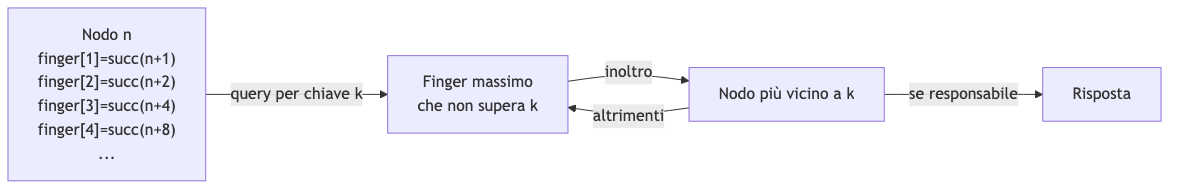
\includegraphics[keepaspectratio,alt={Diagramma Mermaid}]{images/mermaid-lezione-3-retrieving-content-e-dht-03.png}}
\emph{Fig. --- Il meccanismo della finger table: ogni hop dimezza la
distanza residua alla chiave cercata, portando il costo totale a
\(O(\log N)\) hop.}

\begin{callouttip}{Scala del miglioramento}

Con \(N = 10^6\) nodi: - Routing sequenziale: fino a \textbf{500.000
hop} - Finger table: \(\log_2(10^6) \approx\) \textbf{20 hop}

Il miglioramento è di cinque ordini di grandezza. Sia la routing table
che il numero di hop sono \(O(\log N)\).

\end{callouttip}

\begin{center}\rule{0.5\linewidth}{0.5pt}\end{center}

\section{Chord}\label{chord}

\textbf{Chord} è il DHT di riferimento costruito esattamente sui
principi illustrati. Fu sviluppato nel 2001 da un gruppo di ricerca
formato da ricercatori del MIT e dell'Università della California (Ion
Stoica, Robert Morris, David Liben-Nowell, David R. Karger, M. Frans
Kaashoek, Frank Dabek, Hari Balakrishnan) e pubblicato su IEEE/ACM
Transactions on Networking con il titolo \emph{``Chord: A Scalable
Peer-to-peer Lookup Protocol for Internet Applications''}.

La topologia di Chord è un anello con \emph{chord} --- le scorciatoie
della finger table sono i ``chord'' che danno il nome al sistema. Ogni
nodo mantiene un puntatore al predecessore (per le operazioni di
join/leave) e la finger table per il routing efficiente.

\begin{calloutnote}{Varianti di DHT}

Diverse proposte ``consistent-hashing compliant'' differiscono nel modo
in cui i dati vengono associati ai peer e nell'operatore usato per
trovare il peer responsabile di una chiave (\texttt{FindPeer} o
\texttt{FindSuccessor}). Esempi notevoli: \textbf{CAN}
(Content-Addressable Network), \textbf{Chord}, \textbf{Pastry},
\textbf{Tapestry}, \textbf{Kademlia}. I termini ``Structured
Peer-to-Peer'' e ``DHT'' sono spesso usati come sinonimi.

\end{calloutnote}

\begin{center}\rule{0.5\linewidth}{0.5pt}\end{center}

\section{Location Addressing vs Content
Addressing}\label{location-addressing-vs-content-addressing}

Il \textbf{location addressing} è il metodo classico di Internet: un
link HTTP punta a una specifica posizione su uno o più server.
L'identità del dato è dove si trova, non cosa contiene. Chi controlla
quella posizione controlla il contenuto: anche se migliaia di persone
hanno scaricato una copia di un dato, HTTP punta a una sola posizione
fisica. Il web tradizionale ci costringe a fingere che i dati esistano
in un unico posto, con tutte le implicazioni di censura, disponibilità e
controllo che ne derivano.

Il \textbf{content addressing} rovescia il paradigma: il contenuto viene
identificato dalla propria \emph{impronta} crittografica --- il suo hash
--- anziché dalla sua posizione. Avere l'hash di un contenuto permette
di ottenerlo da chiunque ne abbia una copia, indipendentemente da dove
si trova. L'hash non cambia mai, quindi i link restano validi qualunque
sia la fonte, chiunque abbia aggiunto il contenuto, e quando è stato
aggiunto.

\begin{callouttip}{Implicazioni del Content Addressing}

Nel content addressing il link è una \emph{garanzia di integrità}: se
ricevo dati il cui hash corrisponde alla chiave cercata, so che sono
esattamente quelli che volevo, senza dovermi fidare della sorgente. Non
è possibile ricevere contenuti contraffatti spacciandoli per la chiave
corretta.

\end{callouttip}

Questo approccio è alla base di \textbf{IPFS} (\emph{InterPlanetary File
System}), la rete P2P che implementa Web3, il web distribuito. I dati
non sono più delegati a server centrali (Facebook, Instagram, Dropbox),
ma memorizzati in un ambiente P2P distribuito dove chiunque può
recuperare un contenuto da chiunque lo abbia.

\subsection{Content Lookup}\label{content-lookup}

In un sistema basato su content addressing, il routing è
\emph{content-based}: ogni nodo mantiene una routing table che
rappresenta una visione parziale della rete. Quando si cerca un dato con
hash \(k\), il messaggio viene instradato hop-by-hop verso il nodo
responsabile di \(k\), con ciascun hop che si avvicina alla
destinazione. Il numero di hop necessari è \(O(\log N)\), con routing
table di dimensione \(O(\log N)\) per ogni nodo.

\begin{center}\rule{0.5\linewidth}{0.5pt}\end{center}

\section{API della DHT}\label{api-della-dht}

Le DHT espongono intenzionalmente un'interfaccia minimale, indipendente
dall'applicazione:

\begin{itemize}
\tightlist
\item
  \texttt{PUT(key,\ value)} --- inserisce un valore associato a una
  chiave
\item
  \texttt{GET(key)} → \texttt{value} --- recupera il valore associato a
  una chiave
\end{itemize}

Non esiste generalmente una funzione esplicita per spostare le chiavi.
Il valore associato a una chiave può essere un file, un indirizzo IP, un
riferimento a un peer, o qualsiasi altro dato, a seconda
dell'applicazione che usa la DHT come strato infrastrutturale.

\pandocbounded{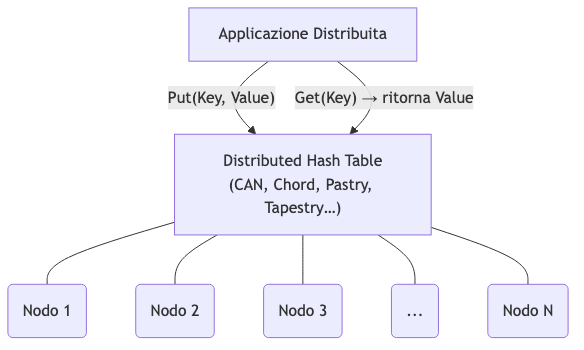
\includegraphics[keepaspectratio,alt={Diagramma Mermaid}]{images/mermaid-lezione-3-retrieving-content-e-dht-04.png}}
\emph{Fig. --- L'API della DHT espone solo Put e Get all'applicazione,
nascondendo completamente la complessità della distribuzione.}

\begin{center}\rule{0.5\linewidth}{0.5pt}\end{center}

\section{Load Balancing e Virtual
Server}\label{load-balancing-e-virtual-server}

Il load imbalance in una DHT ha tre cause distinte:

\begin{enumerate}
\def\labelenumi{\arabic{enumi}.}
\tightlist
\item
  \textbf{Spazio non uniforme}: un nodo gestisce una porzione di spazio
  di indirizzi più grande degli altri --- risolvibile con una funzione
  hash uniforme.
\item
  \textbf{Dati pesanti}: lo spazio è distribuito uniformemente, ma il
  nodo gestisce una \emph{quantità} di dati molto maggiore (le chiavi
  assegnategli corrispondono a file grandi).
\item
  \textbf{Query concentrate}: lo spazio è distribuito uniformemente, ma
  il nodo riceve molte più query perché i dati assegnatigli sono molto
  popolari (\emph{hotspot}).
\end{enumerate}

Il load imbalance produce: minore robustezza del sistema, minore
scalabilità, e impossibilità di garantire i bound \(O(\log N)\).

La soluzione standard è usare i \textbf{virtual server}: ogni nodo
fisico mantiene più identità sull'anello --- ossia è responsabile di più
intervalli non contigui --- distribuendo la responsabilità delle chiavi
in modo più uniforme. Questo mitiga principalmente i problemi di tipo 1
e parzialmente di tipo 3, ma non risolve completamente il problema degli
hotspot dovuti a contenuti virali.

\begin{center}\rule{0.5\linewidth}{0.5pt}\end{center}

\section{Sfide Aperte delle DHT}\label{sfide-aperte-delle-dht}

\begin{calloutwarning}{DHT Challenges}

\begin{itemize}
\tightlist
\item
  \textbf{Hotspot}: distribuire le responsabilità in modo uniforme per
  evitare che alcuni nodi siano molto più carichi di altri. I virtual
  server aiutano, ma un contenuto estremamente popolare resterà sempre
  un collo di bottiglia per il nodo responsabile.
\item
  \textbf{Churn}: redistribuire le responsabilità quando i nodi si
  connettono o disconnettono. In una rete P2P reale il churn è continuo
  e ad alta frequenza --- ogni operazione di join/leave deve essere
  gestita senza interrompere il servizio.
\item
  \textbf{Trade-off strutturale}: dimensione delle routing table vs
  traffico nell'overlay vs \emph{stretch} rispetto all'underlay. I
  percorsi logici nella DHT possono essere molto più lunghi dei percorsi
  fisici ottimali sulla rete sottostante --- un nodo logicamente vicino
  può essere fisicamente a mezzo mondo di distanza.
\end{itemize}

\end{calloutwarning}

\begin{center}\rule{0.5\linewidth}{0.5pt}\end{center}

\section{Confronto tra Architetture}\label{confronto-tra-architetture}

{\def\LTcaptype{none} % do not increment counter
\begin{longtable}[]{@{}
  >{\raggedright\arraybackslash}p{(\linewidth - 10\tabcolsep) * \real{0.3063}}
  >{\raggedright\arraybackslash}p{(\linewidth - 10\tabcolsep) * \real{0.1441}}
  >{\raggedright\arraybackslash}p{(\linewidth - 10\tabcolsep) * \real{0.1982}}
  >{\raggedright\arraybackslash}p{(\linewidth - 10\tabcolsep) * \real{0.1351}}
  >{\raggedright\arraybackslash}p{(\linewidth - 10\tabcolsep) * \real{0.1261}}
  >{\raggedright\arraybackslash}p{(\linewidth - 10\tabcolsep) * \real{0.0901}}@{}}
\toprule\noalign{}
\begin{minipage}[b]{\linewidth}\raggedright
Approccio
\end{minipage} & \begin{minipage}[b]{\linewidth}\raggedright
Memoria per nodo
\end{minipage} & \begin{minipage}[b]{\linewidth}\raggedright
Overhead comunicazione
\end{minipage} & \begin{minipage}[b]{\linewidth}\raggedright
Query complesse
\end{minipage} & \begin{minipage}[b]{\linewidth}\raggedright
Falsi negativi
\end{minipage} & \begin{minipage}[b]{\linewidth}\raggedright
Robustezza
\end{minipage} \\
\midrule\noalign{}
\endhead
\bottomrule\noalign{}
\endlastfoot
\textbf{Server Centralizzato} & \(O(N)\) & \(O(1)\) & Sì & Si & No
(SPOF) \\
\textbf{P2P Non Strutturato (flooding)} & \(O(1)\) & \(O(N^2)\) & Sì &
No & Sì \\
\textbf{DHT} & \(O(\log N)\) & \(O(\log N)\) & No & Si & Sì \\
\end{longtable}
}

\begin{center}\rule{0.5\linewidth}{0.5pt}\end{center}

\section{Applicazioni delle DHT}\label{applicazioni-delle-dht}

Le DHT offrono un servizio generico di memorizzazione e indicizzazione
distribuita. Il valore associato a una chiave può essere un file, un
indirizzo IP, o qualsiasi altro dato --- la semantica dipende
dall'applicazione. Esempi concreti di sistemi che usano DHT:

\begin{itemize}
\tightlist
\item
  \textbf{IPFS} (\emph{InterPlanetary File System}): file system
  distribuito content-addressed, base di Web3
\item
  \textbf{BitTorrent}: memorizzazione dei riferimenti ai peer in uno
  swarm (il DHT di BitTorrent è basato su Kademlia)
\item
  \textbf{Ethereum}: memorizzazione dei riferimenti ai peer nella rete
  P2P sottostante al protocollo
\item
  Supporto a servizi di livello superiore: qualsiasi applicazione che
  necessiti di un registro distribuito di chiave/valore
\end{itemize}

\begin{center}\rule{0.5\linewidth}{0.5pt}\end{center}

\begin{calloutnote}{Sintesi}

Le DHT sono sistemi auto-organizzanti, semplici ed efficienti. Il
routing è basato su chiave; le chiavi sono distribuite uniformemente tra
i nodi, garantendo bottleneck avoidance, inserimento incrementale e
fault tolerance. La realizzazione concreta di questo modello tramite
consistent hashing con finger table (Chord) porta a una struttura con
\(O(\log N)\) hop per il lookup e \(O(\log N)\) entry nella routing
table per nodo. I termini ``Structured Peer-to-Peer'' e ``DHT'' sono
spesso usati come sinonimi.

\end{calloutnote}

\begin{center}\rule{0.5\linewidth}{0.5pt}\end{center}

\newpage

\chapter{Kademlia}\label{kademlia}

\section{Panoramica}\label{panoramica}

Kademlia è un protocollo DHT progettato da Maymounkov e Mazières nel
2002. Il nome viene dal bulgaro: è il nome di una vetta montuosa in
Bulgaria, nonché una parola turca per ``uomo fortunato''. È considerato
lo standard de facto per le reti P2P su Internet ed è adottato da
Ethereum, IPFS (nelle varianti S/Kademlia e Sloppy Kademlia), BitTorrent
(Mainline DHT) ed eMule (rete KAD).

Kademlia presenta caratteristiche che non sono offerte da nessun'altra
DHT esistente: - Le informazioni di routing si diffondono
\textbf{automaticamente} come effetto collaterale dei lookup, senza
messaggi dedicati - Supporta il \textbf{parallel routing} (richieste
multiple in parallelo) per ridurre latenza e timeout - Usa un'unica
metrica --- lo \textbf{XOR} --- per calcolare distanze, instradare
messaggi e organizzare la routing table - È \textbf{fault tolerant}: se
uno o più peer abbandonano la rete, i dati --- replicati su più peer ---
restano recuperabili - Non richiede motori di database complessi: i dati
sono coppie chiave-valore, quindi anche dispositivi IoT con storage
limitato possono partecipare

\begin{center}\rule{0.5\linewidth}{0.5pt}\end{center}

\section{Chord: Riepilogo}\label{chord-riepilogo}

In Chord i nodi scelgono un ID quasi uniformemente casuale nell'anello.
Gli identificatori sull'anello vengono chiamati \textbf{chiavi} (per
distinguerli dagli ID dei nodi). Ogni blocco contiguo dell'anello è
assegnato a un nodo. Un nodo con identificatore ID mantiene puntatori
verso i nodi \texttt{successor(ID\ +\ 2\^{}i)} per potenze di 2 fino a
\(2^m\) (finger table), dove \(m\) è il numero di bit degli
identificatori.

\begin{center}\rule{0.5\linewidth}{0.5pt}\end{center}

\section{Spazio degli Identificatori}\label{spazio-degli-identificatori}

Sia i nodi che i contenuti sono identificati da hash a \(M\) bit. Lo
spazio di tutti i possibili identificatori è visualizzato come un
\textbf{trie binario completo}: ogni livello rappresenta un bit, ogni
nodo interno ha al più due figli (figlio sinistro → bit 0, figlio destro
→ bit 1), e ogni foglia rappresenta un identificatore completo.
\pandocbounded{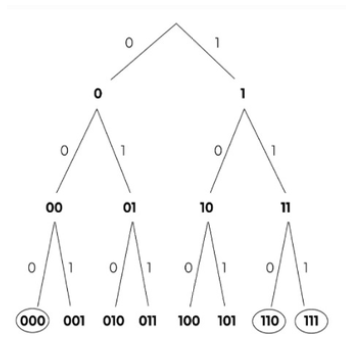
\includegraphics[keepaspectratio]{images/Pasted-image-20260407111031.png}}
In pratica, lo spazio degli identificatori è enorme e i nodi che
partecipano alla DHT sono molto meno degli identificatori possibili. Il
\textbf{node tree} è una vista alternativa al trie completo: un albero
binario non bilanciato che mostra solo le foglie corrispondenti ai nodi
effettivamente presenti nella rete. Una foglia del node tree corrisponde
a un \textbf{prefisso identificatore} che identifica univocamente quel
peer --- ovvero il prefisso più corto che non è condiviso da nessun
altro peer nell'overlay.

\subsection{Mappatura delle Chiavi ai
Nodi}\label{mappatura-delle-chiavi-ai-nodi}

Per assegnare una chiave (identificatore di un dato) a un nodo, Kademlia
usa il \textbf{Lowest Common Ancestor (LCA)}: il punto più profondo
dell'albero in cui il percorso della chiave e quello del nodo coincidono
prima di biforcarsi. La chiave viene assegnata al nodo con LCA più
profondo con essa.

In caso di parità tra due nodi che hanno lo stesso LCA rispetto a una
chiave, si spezza il pareggio guardando il bit più significativo in cui
i due nodi differiscono (il suo indice è \(b\)): la chiave viene
assegnata al nodo il cui \(b\)-esimo bit coincide con il \(b\)-esimo bit
della chiave.

\begin{callouttip}{Tie-breaking}

Peer 110 e 111 hanno lo stesso LCA rispetto alla chiave 101. I due peer
differiscono al terzo bit. Poiché il terzo bit di 101 è 1, la chiave 101
viene assegnata al nodo 111.

\end{callouttip}

\begin{center}\rule{0.5\linewidth}{0.5pt}\end{center}

\section{La Metrica XOR}\label{la-metrica-xor}

\subsection{Derivazione}\label{derivazione}

Per trovare il nodo più vicino a una chiave, si può usare un algoritmo
brute-force: si esaminano tutti gli ID dei nodi bit per bit dal più
significativo al meno significativo; ad ogni posizione, se almeno un
candidato ha lo stesso bit della chiave, si eliminano quelli che
differiscono. La complessità è \(O(n \cdot m)\).

Un approccio più elegante: si definisce un valore scalare di distanza
che penalizza le differenze ai bit più significativi più di tutte le
differenze ai bit meno significativi messe insieme. Poiché
\(2^i > \sum_{j=0}^{i-1} 2^j\), la penalità giusta per una differenza al
\(i\)-esimo bit è \(2^i\). Questo è esattamente ciò che fa l'operazione
\textbf{XOR}.

\begin{calloutdefinition}{Distanza XOR}

La distanza tra due identificatori \(x\) e \(y\) è definita come
\(d(x, y) = x \oplus y\). Un contenuto viene memorizzato sul nodo con
distanza XOR minima rispetto alla sua chiave.

\end{calloutdefinition}

\begin{calloutwarning}{XOR ≠ distanza numerica}

Due identificatori possono essere vicini numericamente ma lontani
secondo la metrica XOR: \(1000 \oplus 0111 = 1111 = 15\) (distanza XOR
massima), mentre la differenza numerica è solo 1. La metrica XOR si basa
sull'albero binario, non sulla linea numerica.

\end{calloutwarning}

\subsection{Proprietà della Metrica
XOR}\label{proprietuxe0-della-metrica-xor}

La metrica XOR soddisfa le proprietà di una metrica formale:

\begin{itemize}
\tightlist
\item
  \(d(x, x) = 0\)
\item
  \(d(x, y) > 0\) se \(x \neq y\)
\item
  \textbf{Simmetria} --- \(d(x,y) = d(y,x)\). Se \(A\) vede \(B\) come
  vicino, anche \(B\) vede \(A\) come vicino. Questo permette a entrambi
  di apprendere informazioni di routing dall'altro gratuitamente. In
  Chord questo non vale: se \(x\) riceve una query da \(y\), \(y\) ha
  \(x\) nella sua finger table, ma \(x\) potrebbe non avere \(y\) come
  finger → le informazioni nelle query ricevute non possono arricchire
  la finger table.
\item
  \textbf{Disuguaglianza triangolare} ---
  \(d(x,z) \le d(x,y) + d(y,z)\). Andare direttamente da \(x\) a \(z\) è
  sempre almeno comodo quanto passare per \(y\). Segue dalla
  transitività: \(d(x,y) \oplus d(y,z) = d(x,z)\).
\item
  \textbf{Unidirezionalità} --- Dato un nodo \(x\) e una distanza
  \(\Delta\), esiste un \textbf{unico} nodo \(y\) tale che
  \(d(x,y) = \Delta\). Esempio: \(x = 1001\), \(\Delta = 0001\), l'unico
  punto a distanza \(\Delta\) da \(x\) è \(y = 1000\). Le ricerche per
  la stessa chiave convergono sempre sullo stesso percorso, permettendo
  di usare \textbf{cache lungo la rotta} per evitare hotspot.
\end{itemize}

\subsection{Relazione tra Prefisso Comune e
Distanza}\label{relazione-tra-prefisso-comune-e-distanza}

La metrica XOR è legata al prefisso identificatore: più lungo è il
prefisso comune tra due nodi, minore è la loro distanza XOR. Due
identificatori che condividono un prefisso di lunghezza \(p\) e
differiscono negli ultimi \(i = L - p\) bit hanno distanza XOR:

\[2^{i-1} \le d(x,y) < 2^i\]

\begin{callouttip}{Subtree distances}

\(X = 010110\), \(Y = 011110\), \(X \oplus Y = 001000\),
\(d(x,y) = 2^3 = 8\) (minima per quel sottalbero).

Due foglie nei due sottoalberi opposti (prefisso comune = 0):
\(0111 \oplus 1000 = 1111 = 15\) (massima),
\(0111 \oplus 1111 = 1000 = 8\) (minima).

\end{callouttip}

\begin{center}\rule{0.5\linewidth}{0.5pt}\end{center}

\section{Routing Table e K-Buckets}\label{routing-table-e-k-buckets}

\subsection{Struttura}\label{struttura}

\begin{calloutdefinition}{K-Bucket}

Lista di al massimo \(k\) contatti, ognuno memorizzato come tripla
\texttt{(Node\ ID,\ IP\ address,\ UDP\ port)}. I contatti sono ordinati
per recency: il meno recente in testa, il più recente in coda. Il bucket
\(i\) contiene contatti con distanza XOR \(d \in [2^{i-1}, 2^i)\) dal
nodo proprietario.

\end{calloutdefinition}

Ogni nodo mantiene una routing table di \(M\) bucket (uno per ogni
sottoalbero dal punto di vista del nodo). I bucket per distanze piccole
(lunga prefix comune) tendono ad avere pochi contatti --- ci sono pochi
nodi in quel vicinato. I bucket per distanze grandi coprono porzioni
enormi dello spazio e sono generalmente pieni. Ad ogni passo di routing,
la query si avvicina di almeno un bit al target: costo totale
\(O(\log N)\) --- è il \textbf{prefix match routing}.

\pandocbounded{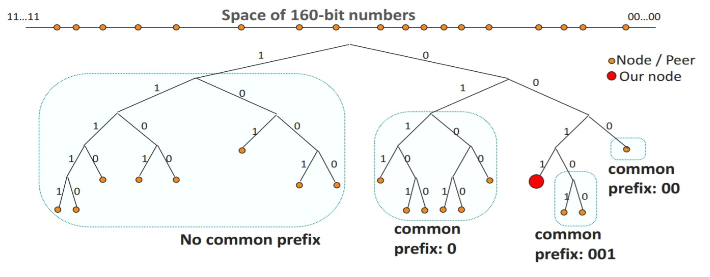
\includegraphics[keepaspectratio]{images/Pasted-image-20260407111152.png}}
Il parametro \(k\) è scelto in modo che la probabilità di \(k\) guasti
simultanei sia trascurabile.

\subsection{Aggiornamento dei
K-Buckets}\label{aggiornamento-dei-k-buckets}

Quando arriva un messaggio da un nodo:

\begin{verbatim}
if sender già nel bucket:
    sposta sender in coda (più recente)
else if bucket non pieno:
    inserisci sender in coda
else:
    ping al nodo in testa (il meno recente)
    if non risponde:
        rimuovi il nodo in testa, inserisci sender in coda
    else:
        sposta il nodo in testa in coda, scarta sender
\end{verbatim}

Questa politica \textbf{favorisce i nodi vecchi}: l'analisi di tracce
Gnutella mostra che più a lungo un nodo è rimasto online, più è
probabile che continui a farlo (\emph{least recently seen eviction}). Ne
derivano due vantaggi: - La routing table è stabile e punta a nodi
affidabili - \textbf{Resistenza ai DoS}: un attaccante non può svuotare
la routing table inviando messaggi da nodi fasulli, perché i nuovi
contatti vengono inseriti solo se i vecchi scompaiono

\subsection{Refresh Periodico}\label{refresh-periodico}

I k-bucket vengono aggiornati automaticamente dal traffico dei messaggi.
Tuttavia, se un bucket non riceve messaggi per un certo periodo,
Kademlia esegue un \textbf{refresh} orario: sceglie un ID casuale nel
range del bucket e vi effettua una ricerca. Se il nodo con quell'ID
risponde, viene inserito nel bucket.

\begin{center}\rule{0.5\linewidth}{0.5pt}\end{center}

\section{Primitive del Protocollo}\label{primitive-del-protocollo}

Kademlia espone quattro RPC su \textbf{UDP}:

{\def\LTcaptype{none} % do not increment counter
\begin{longtable}[]{@{}
  >{\raggedright\arraybackslash}p{(\linewidth - 2\tabcolsep) * \real{0.5000}}
  >{\raggedright\arraybackslash}p{(\linewidth - 2\tabcolsep) * \real{0.5000}}@{}}
\toprule\noalign{}
\begin{minipage}[b]{\linewidth}\raggedright
Primitiva
\end{minipage} & \begin{minipage}[b]{\linewidth}\raggedright
Descrizione
\end{minipage} \\
\midrule\noalign{}
\endhead
\bottomrule\noalign{}
\endlastfoot
\texttt{PING} & Verifica se un nodo è online \\
\texttt{STORE(key,\ value)} & Istruisce un nodo a memorizzare una coppia
chiave-valore \\
\texttt{FIND\_NODE(target)} & Restituisce \(k\) triple
\texttt{(ID,\ IP,\ UDP\ port)} per i \(k\) nodi più vicini al target.
Può attingere da un singolo bucket o da più bucket se il più vicino non
è pieno; restituisce sempre \(k\) elementi, salvo che il nodo conosca
meno di \(k\) nodi in totale \\
\texttt{FIND\_VALUE(key)} & Se il nodo possiede il valore corrispondente
a \texttt{key}, lo restituisce direttamente. Altrimenti si comporta come
\texttt{FIND\_NODE} e restituisce \(k\) triple; spetta al richiedente
continuare la ricerca \\
\end{longtable}
}

\begin{center}\rule{0.5\linewidth}{0.5pt}\end{center}

\section{Lookup Iterativo e
Parallelo}\label{lookup-iterativo-e-parallelo}

\subsection{Tipi di Lookup}\label{tipi-di-lookup}

Un lookup in Kademlia è una procedura di ricerca distribuita che si
avvicina progressivamente a un ID target nello spazio XOR. Il target può
essere: - Un \textbf{node ID} (node lookup): usato per mantenere le
routing table e trovare il nodo in cui memorizzare un dato - Un
\textbf{key ID} (value lookup): usato per recuperare il valore associato
a una chiave

\subsection{Procedura a 3 step}\label{procedura-a-3-step}

\begin{enumerate}
\def\labelenumi{\arabic{enumi}.}
\tightlist
\item
  Il nodo iniziatore trova il nodo più vicino al target nella propria
  routing table (tramite distanza XOR)
\item
  Invia la query a quel nodo chiedendo nodi più vicini al target
\item
  Ripete il processo con i nodi più vicini ricevuti
\end{enumerate}

Il lookup si ferma quando: nessuna risposta restituisce nodi più vicini
di quelli già noti, oppure il nodo più vicino noto è già stato
interrogato. Ad ogni iterazione, la metrica XOR si riduce della metà ---
il numero di hop è \(O(\log N)\).

\subsection{Routing Parallelo (α)}\label{routing-parallelo-ux3b1}

Il parametro \(\alpha\) controlla la concorrenza: invece di aspettare un
nodo alla volta, si interrogano \(\alpha\) nodi simultaneamente. Questo
riduce la latenza totale e rende il sistema robusto ai nodi lenti o
offline.

\begin{callouttip}{Utilità del parallel routing}

Il nodo blu 0011 cerca il nodo rosso 1101. Conosce i nodi verdi 1001 e
1110. \(d(1101, 1001) = 4\), \(d(1101, 1110) = 3\). Il nodo 1001 è più
distante, ma potrebbe conoscere il target mentre 1110 non lo conosce.
Con routing parallelo, 0011 invia la query a entrambi simultaneamente.

\end{callouttip}

\begin{calloutwarning}{Il nodo più vicino non è necessariamente il percorso più breve}

Dati \(x\), \(y\), \(z\) con \(d(y,x) < d(z,x)\): è possibile che \(z\)
conosca \(x\) mentre \(y\) non lo conosce. L'unidirezionalità della
metrica XOR garantisce che tutti i percorsi convergano verso il target,
quindi inviare la query a \(\geq 1\) nodi più vicini è sufficiente.

\end{calloutwarning}

Quando \(\alpha = 1\) il lookup è simile a Chord (un passo alla volta);
con \(\alpha > 1\) Kademlia ha la flessibilità di scegliere tra \(k\)
nodi a ogni passo.

\subsection{Algoritmo Completo}\label{algoritmo-completo}

\begin{verbatim}
k-closest ← α contatti dal k-bucket non vuoto più vicino alla chiave
             (se meno di α, si aggiungono contatti da bucket adiacenti)
closestNode ← il nodo più vicino in k-closest

repeat:
    seleziona α contatti da k-closest non ancora interrogati
    invia FIND_NODE in parallelo e in modo asincrono
    ogni contatto vivo risponde con k nodi
    aggiungi i nuovi nodi a k-closest, aggiorna closestNode
until nessun nodo più vicino di closestNode viene restituito

invia FIND_NODE in parallelo ai k nodi più vicini non ancora interrogati
return k nodi più vicini
\end{verbatim}

\begin{center}\rule{0.5\linewidth}{0.5pt}\end{center}

\section{Join, Store e Leave}\label{join-store-e-leave}

\subsection{Ingresso nella rete (Join)}\label{ingresso-nella-rete-join}

\begin{enumerate}
\def\labelenumi{\arabic{enumi}.}
\tightlist
\item
  Il nuovo nodo contatta un \textbf{bootstrap node} noto; la routing
  table iniziale contiene solo la coppia
  \texttt{(nuovo\ nodo,\ bootstrap\ node)} in un unico bucket
\item
  Esegue \texttt{FIND\_NODE(proprio\ ID)} → scopre nodi vicini a sé,
  riempie i bucket ad alto indice, e si fa conoscere dagli altri nodi
\item
  Esegue \texttt{FIND\_NODE(ID\ casuale)} per bucket sempre più distanti
  dal proprio, arricchendo progressivamente tutti i bucket
\end{enumerate}

La flessibilità di questa procedura è superiore rispetto a Chord, che
richiede passi di join più rigidi.

\subsection{Archiviazione di un dato
(Store)}\label{archiviazione-di-un-dato-store}

\begin{enumerate}
\def\labelenumi{\arabic{enumi}.}
\tightlist
\item
  Si esegue un lookup per trovare i \(k\) nodi con ID più vicini alla
  chiave
\item
  Si invia \texttt{STORE} a tutti i \(k\) nodi → il dato è replicato
  \(k\) volte
\end{enumerate}

\textbf{Pubblicazione periodica}: i dati sono \emph{soft-state} e devono
essere rinfrescati. Il nodo che ha pubblicato un dato deve
\textbf{ripubblicare periodicamente} per contrastare il churn. Nella
versione per file sharing, la ripubblicazione avviene ogni 24 ore.
Ottimizzazione: se un nodo riceve un \texttt{STORE}, suppone che sia
stato inviato anche ai vicini stretti e non ripubblica nell'ora
successiva, riducendo i messaggi scambiati.

\textbf{Caching lungo il percorso}: i valori vengono \textbf{cached} nel
primo nodo sul percorso di lookup che non li conosceva. Questo aiuta a
distribuire il carico per dati molto popolari.

\subsection{Disconnessione (Leave)}\label{disconnessione-leave}

La disconnessione non richiede operazioni esplicite: se un nodo non
risponde, viene silenziosamente rimosso dai k-bucket degli altri nodi.

\begin{center}\rule{0.5\linewidth}{0.5pt}\end{center}

\section{Kademlia vs Chord}\label{kademlia-vs-chord}

{\def\LTcaptype{none} % do not increment counter
\begin{longtable}[]{@{}
  >{\raggedright\arraybackslash}p{(\linewidth - 4\tabcolsep) * \real{0.3333}}
  >{\raggedright\arraybackslash}p{(\linewidth - 4\tabcolsep) * \real{0.3333}}
  >{\raggedright\arraybackslash}p{(\linewidth - 4\tabcolsep) * \real{0.3333}}@{}}
\toprule\noalign{}
\begin{minipage}[b]{\linewidth}\raggedright
Aspetto
\end{minipage} & \begin{minipage}[b]{\linewidth}\raggedright
Chord
\end{minipage} & \begin{minipage}[b]{\linewidth}\raggedright
Kademlia
\end{minipage} \\
\midrule\noalign{}
\endhead
\bottomrule\noalign{}
\endlastfoot
\textbf{Metrica} & Distanza numerica (anello) & XOR \\
\textbf{Simmetria} & No --- finger table asimmetriche & Sì ---
apprendimento mutuale gratuito \\
\textbf{Routing} & Ricorsivo & Iterativo + parallelo (\(\alpha\)
nodi) \\
\textbf{Lookup} & \(O(\log N)\) hop & \(O(\log N)\) hop \\
\textbf{Aggiornamento routing table} & Messaggi dedicati & Effetto
collaterale dei lookup \\
\textbf{Località} & Non considerata & RTT memorizzato per ogni contatto;
preferisce il contatto con RTT minore \\
\textbf{Tolleranza ai guasti} & Limitata & Alta (parallel routing +
bucket policy) \\
\end{longtable}
}

In Chord, se \(x\) riceve una query da \(y\), \(y\) ha \(x\) nella sua
finger table ma \(x\) potrebbe non avere \(y\) come finger --- le
informazioni nelle query ricevute non si possono usare per arricchire la
finger table. In Kademlia la simmetria della metrica permette a ogni
nodo di arricchire la propria routing table attraverso le query che
riceve.

\begin{center}\rule{0.5\linewidth}{0.5pt}\end{center}

\section{Punti di Forza e Debolezze}\label{punti-di-forza-e-debolezze}

\begin{calloutnote}{Strengths}

\begin{itemize}
\tightlist
\item
  Basso overhead di messaggi di controllo
\item
  Tolleranza a guasti e disconnessioni dei nodi
\item
  Selezione di percorsi a bassa latenza (RTT-aware)
\item
  Limiti di prestazione dimostrabili formalmente
\end{itemize}

\end{calloutnote}

\begin{calloutwarning}{Weaknesses}

\begin{itemize}
\tightlist
\item
  Distribuzione non uniforme dei nodi nello spazio degli ID → routing
  table sbilanciata e routing inefficiente
\item
  Bilanciamento del carico di memorizzazione non completamente risolto
\item
  Protocollo originariamente sottospecificato → proliferazione di
  implementazioni diverse
\item
  Difficile produrre risultati analitici precisi
\item
  Risultati di routing non deterministici (tempo, vicinato)
\end{itemize}

\end{calloutwarning}

\newpage

\chapter{Lezione 5 --- (Lab) P2P Networks in Bitcoin ed
Ethereum}\label{lezione-5-lab-p2p-networks-in-bitcoin-ed-ethereum}

\section{Inquadramento della lezione}\label{inquadramento-della-lezione}

Questo primo laboratorio del corso apre la sezione applicativa della
parte P2P: anziché discutere in astratto le proprietà delle reti
overlay, si guarda come due blockchain reali --- Bitcoin ed Ethereum ---
abbiano implementato, ciascuna a modo suo, il livello di comunicazione
peer-to-peer su cui tutto il resto (consenso, propagazione delle
transazioni, sincronizzazione degli stati) si appoggia.

L'obiettivo è fare da ponte tra la teoria vista nelle lezioni iniziali
(classificazione degli overlay, Kademlia, DHT) e ciò che si troverà
effettivamente installando un client Bitcoin Core o un nodo
\texttt{geth}. La chiave di lettura è il confronto: \textbf{Bitcoin ha
scelto un overlay non strutturato} basato su gossip, \textbf{Ethereum
uno strutturato} basato su Kademlia --- due risposte molto diverse allo
stesso problema, scoprire peer con cui parlare senza conoscere la
topologia globale.

\begin{calloutnote}{Informazioni organizzative}

Il modulo di laboratorio segue in modo ``organico'' il modulo teorico:
la scaletta degli argomenti si adatta a quelli già visti a lezione. Il
materiale di riferimento è costituito dai link inseriti nelle slide di
ogni laboratorio, e le domande possono essere poste in ufficio (333 Dip.
Informatica) o via Teams su richiesta. Ogni studente lavora con il
proprio dispositivo (\emph{bring your own device}).

\end{calloutnote}

\begin{center}\rule{0.5\linewidth}{0.5pt}\end{center}

\section{Il problema di base delle reti
P2P}\label{il-problema-di-base-delle-reti-p2p}

Prima di confrontare i due approcci conviene ricordare qual è il
problema comune. In una rete peer-to-peer un nodo possiede \textbf{solo
informazioni topologiche locali}: non conosce --- e, per ragioni di
privacy e resistenza agli attacchi, \textbf{non deve} conoscere --- la
topologia complessiva. Ogni partecipante vede soltanto i propri vicini
diretti.

Questa limitazione non è solo una scelta di design: è un requisito di
sicurezza. Una rete in cui ogni nodo pubblica la lista completa dei peer
sarebbe banalmente attaccabile, perché un avversario potrebbe
ricostruire mappature globali e scegliere bersagli mirati.

Una rete P2P ben progettata deve essere resistente ad almeno tre
famiglie di attacchi:

\begin{itemize}
\tightlist
\item
  \textbf{Sybil attack}: l'avversario crea un numero arbitrario di
  identità fittizie per influenzare la rete (routing, consenso, gossip)
\item
  \textbf{Eclipse attack}: l'avversario circonda un nodo vittima con
  peer sotto il suo controllo, isolandolo dal resto della rete
\item
  \textbf{Partizionamento}: l'avversario divide la rete in componenti
  non comunicanti, permettendo ad esempio di presentare stati divergenti
  a due sottoinsiemi di vittime
\end{itemize}

\begin{calloutwarning}{Bootstrapping problem}

Come fa un nodo appena avviato a scoprire il primo peer a cui
connettersi, se per definizione non conosce nessuno? Questa
``gallina-uovo'' è nota come \textbf{bootstrapping problem} e viene
tipicamente risolta con una lista di nodi di fiducia hardcoded nel
client o con query DNS. È un punto di fragilità: chi controlla quei seed
controlla potenzialmente anche chi riesce a entrare nella rete.

\end{calloutwarning}

La scelta architetturale fondamentale, fatta questa premessa, è fra due
famiglie di overlay:

\pandocbounded{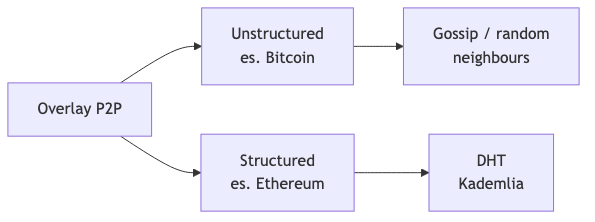
\includegraphics[keepaspectratio,alt={Diagramma Mermaid}]{images/mermaid-lezione-5-lab-p2p-networks-in-bitcoin-ed-ethereum-01.png}}
\emph{Fig. --- Le due grandi famiglie di overlay P2P utilizzate dalle
principali blockchain.}

In entrambi i casi lo scopo è lo stesso: \textbf{abilitare la
comunicazione per un'applicazione decentralizzata}. Le strade scelte per
raggiungerlo sono molto diverse.

\begin{center}\rule{0.5\linewidth}{0.5pt}\end{center}

\section{Bitcoin: overlay non strutturato e
gossip}\label{bitcoin-overlay-non-strutturato-e-gossip}

\subsection{Struttura generale}\label{struttura-generale}

Bitcoin --- almeno nella sua forma attuale, senza considerare Lightning
--- è una \textbf{rete di comunicazione P2P il cui unico scopo è
scambiarsi informazioni su uno stato globale condiviso}. Le informazioni
sono transazioni e blocchi; lo stato globale è il set UTXO.

Le scelte progettuali del livello network di Bitcoin si possono
riassumere così:

{\def\LTcaptype{none} % do not increment counter
\begin{longtable}[]{@{}ll@{}}
\toprule\noalign{}
Aspetto & Scelta di Bitcoin \\
\midrule\noalign{}
\endhead
\bottomrule\noalign{}
\endlastfoot
Overlay & Non strutturato, \textbf{gossip} \\
Bootstrapping & Lista DNS + hardcoded \\
Privacy & Randomizzazione (nessuna geolocalizzazione) \\
Sicurezza & Connessioni cifrate solo dalla v27+ (apr. 2024) \\
Trasporto & TCP \\
\end{longtable}
}

\begin{calloutnote}{Cifratura tardiva}

Fino all'aprile 2024 le connessioni tra nodi Bitcoin erano in chiaro.
Questo permetteva, a chi era posizionato sulla rete (ISP, punti di
interscambio), di distinguere facilmente il traffico Bitcoin e fare
fingerprinting. La v27 introduce finalmente il supporto nativo al
cifrato, con BIP 324.

\end{calloutnote}

\subsection{Node discovery in Bitcoin}\label{node-discovery-in-bitcoin}

Un nodo appena avviato segue un protocollo relativamente semplice per
entrare a far parte della rete:

\begin{enumerate}
\def\labelenumi{\arabic{enumi}.}
\tightlist
\item
  \textbf{Ottiene una lista di indirizzi candidati} da DNS di fiducia o
  da una lista hardcoded: ad esempio
  \texttt{nslookup\ seed.bitcoin.sipa.be} restituisce gli IP di una
  serie di nodi ``seeder'' mantenuti da sviluppatori noti della
  community. L'elenco hardcoded nel sorgente vive in
  \texttt{src/chainparamsseeds.h}.
\item
  \textbf{Invia un messaggio \texttt{version}} a uno o più di questi
  peer per tentare la connessione.
\item
  Se il peer accetta, risponde con un messaggio \textbf{\texttt{verack}}
  (version acknowledgement).
\item
  Da quel momento il nodo può chiedere altri peer a chi già conosce
  tramite il messaggio \textbf{\texttt{getaddr}}, ricevendo in risposta
  una lista di indirizzi di altri partecipanti alla rete.
\item
  Periodicamente, il nodo \textbf{annuncia se stesso} (cioè invia la
  propria \texttt{addr}) ad alcuni vicini scelti casualmente, così che
  l'informazione della sua presenza si propaghi per gossip.
\end{enumerate}

\pandocbounded{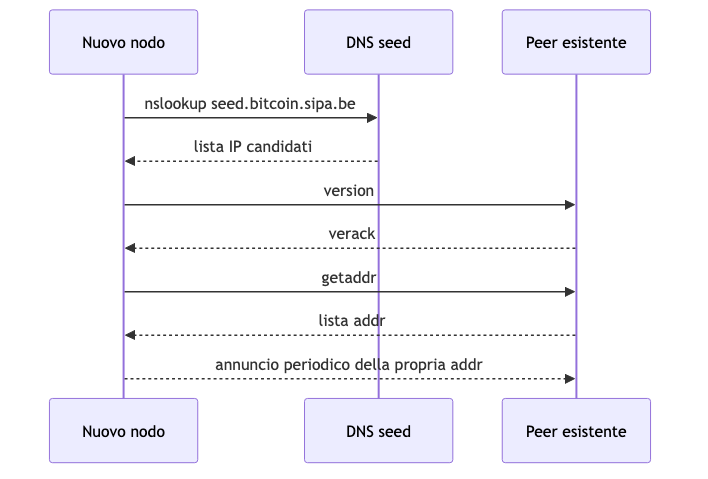
\includegraphics[keepaspectratio,alt={Diagramma Mermaid}]{images/mermaid-lezione-5-lab-p2p-networks-in-bitcoin-ed-ethereum-02.png}}
\emph{Fig. --- Handshake iniziale di un nuovo nodo Bitcoin: dal seed DNS
all'inserimento attivo nella rete.}

Una volta stabilita la rete di vicini, i messaggi applicativi veri e
propri --- transazioni e blocchi --- vengono propagati con un meccanismo
a tre fasi: \texttt{inv} annuncia la disponibilità di un oggetto (un
hash), \texttt{getdata} lo richiede, infine arriva il \texttt{block} o
\texttt{tx}. Tecniche come \textbf{trickle} e \textbf{diffusion}
randomizzano i tempi di propagazione per ridurre la possibilità che un
osservatore risalga al nodo originatore di una transazione.

\subsection{Gestione delle
connessioni}\label{gestione-delle-connessioni}

Un nodo Bitcoin mantiene un numero di connessioni ``target'' tra
\textbf{8 e 11}, e un massimo configurabile (di default \textbf{125}).
Il parametro \texttt{-maxconnections=\textless{}num\textgreater{}}
controlla quest'ultimo. La logica concreta risiede in \texttt{src/net.h}
nel repository di Bitcoin Core.

\begin{callouttip}{Perché 8 connessioni}

Il numero basso non è casuale: pochi peer stabilmente connessi bastano a
garantire la raggiungibilità (ogni messaggio fa solo pochi hop prima di
propagarsi a tutta la rete), limitano il consumo di banda e ---
soprattutto --- rendono più costoso per un avversario circondare un
nodo. Con 125 come limite massimo c'è spazio per accettare connessioni
in ingresso da altri nodi.

\end{callouttip}

\subsection{Monitoraggio della rete}\label{monitoraggio-della-rete}

Essendo Bitcoin una rete aperta, chiunque può scansionarla e tenerne
conteggio. Due strumenti spesso citati:

\begin{itemize}
\tightlist
\item
  \href{https://bitnodes.io/}{bitnodes.io} --- conta i nodi
  raggiungibili e mostra grafici storici
\item
  \href{https://21.ninja/}{21.ninja} --- visualizza la propagazione dei
  blocchi
\end{itemize}

Questi dashboard sono utili in due sensi: danno un'idea di quanti nodi
sono ``full'' (oggi dell'ordine di decine di migliaia) e, guardando la
serie temporale, permettono di correlare eventi (hard fork,
aggiornamenti software) con variazioni nella topologia.

\subsection{Attacchi specifici al layer P2P di
Bitcoin}\label{attacchi-specifici-al-layer-p2p-di-bitcoin}

Oltre ai Sybil/eclipse classici, la scarna sicurezza di rete di Bitcoin
ha prestato il fianco storicamente a:

\begin{itemize}
\tightlist
\item
  \textbf{DNS poisoning} dei seed: se l'attaccante compromette la
  risoluzione DNS di un seed, può imporre a tutti i nuovi nodi una
  visione parziale della rete
\item
  \textbf{Network listening}: l'intercettazione in chiaro del traffico
  (risolta solo con la v27)
\item
  \textbf{Fingerprinting tramite il ``addresses cookie''}: sfruttando il
  modo in cui i nodi memorizzano e ripropagano le \texttt{addr} si può
  ricostruire una mappa implicita dei peer, violando la privacy
  topologica
\end{itemize}

\begin{calloutnote}{Riferimento}

L'articolo di Biryukov et al.~(\url{https://arxiv.org/pdf/1410.6079}) è
un classico su come il livello di rete di Bitcoin leaks informazioni che
minano la privacy degli utenti.

\end{calloutnote}

\begin{center}\rule{0.5\linewidth}{0.5pt}\end{center}

\section{Ethereum: overlay strutturato con
Kademlia}\label{ethereum-overlay-strutturato-con-kademlia}

Ethereum risponde allo stesso problema di Bitcoin --- scambiare
informazioni sullo stato globale --- ma con un impianto più sofisticato,
sia perché nato dopo (con più esperienza di attacchi), sia perché le sue
esigenze applicative (molti sub-protocolli) lo richiedono.

{\def\LTcaptype{none} % do not increment counter
\begin{longtable}[]{@{}ll@{}}
\toprule\noalign{}
Aspetto & Scelta di Ethereum \\
\midrule\noalign{}
\endhead
\bottomrule\noalign{}
\endlastfoot
Overlay & Strutturato, \textbf{Kademlia} \\
Bootstrapping & Lista hardcoded di \emph{bootnodes} \\
Privacy & Randomizzazione nella scelta dei vicini \\
Sicurezza & Connessioni \textbf{autenticate e cifrate} \\
Trasporto & \textbf{UDP} per node discovery, \textbf{TCP} per
comunicazione \\
\end{longtable}
}

\subsection{Perché una DHT per il
P2P}\label{perchuxe9-una-dht-per-il-p2p}

Kademlia è una DHT --- una \emph{distributed hash table} --- e
l'argomento per cui una DHT sia preferibile a un gossip non strutturato
è ormai consolidato:

\begin{itemize}
\tightlist
\item
  \textbf{Decentralizzazione}: non serve coordinarsi per costruire la
  propria tabella di routing
\item
  \textbf{Fault tolerance / dinamismo}: la struttura si adatta al
  \emph{churn} (nodi che entrano ed escono continuamente), entro limiti
  ragionevoli
\item
  \textbf{Scalabilità e load balancing}: la quantità di informazione
  locale cresce come \(O(\log n)\) nel numero di nodi, e il routing
  richiede \(O(\log n)\) hop
\end{itemize}

\begin{callouttip}{Il log magico}

Le DHT ``log/log'' sono il punto di equilibrio ideale: uno stato di
routing piccolo che garantisce comunque latenze basse. Questo è ciò che
permette a una rete con decine di migliaia di nodi Ethereum di
continuare a scoprire peer in tempi ragionevoli.

\end{callouttip}

\subsection{Come Kademlia è adattato in
Ethereum}\label{come-kademlia-uxe8-adattato-in-ethereum}

Le differenze rispetto al Kademlia ``da manuale'' sono interessanti e
riflettono la diversa finalità. In Kademlia tradizionale si usa la DHT
per cercare \textbf{valori associati a chiavi}. In Ethereum \textbf{non
si fanno value lookup}: la DHT serve esclusivamente per trovare peer
vicini --- dove ``vicino'' non significa vicino geograficamente, ma
vicino nello spazio degli identificatori.

{\def\LTcaptype{none} % do not increment counter
\begin{longtable}[]{@{}
  >{\raggedright\arraybackslash}p{(\linewidth - 4\tabcolsep) * \real{0.3333}}
  >{\raggedright\arraybackslash}p{(\linewidth - 4\tabcolsep) * \real{0.3333}}
  >{\raggedright\arraybackslash}p{(\linewidth - 4\tabcolsep) * \real{0.3333}}@{}}
\toprule\noalign{}
\begin{minipage}[b]{\linewidth}\raggedright
Dimensione
\end{minipage} & \begin{minipage}[b]{\linewidth}\raggedright
Kademlia ``classico''
\end{minipage} & \begin{minipage}[b]{\linewidth}\raggedright
Kademlia di Ethereum
\end{minipage} \\
\midrule\noalign{}
\endhead
\bottomrule\noalign{}
\endlastfoot
Chiavi vs nodi & Spazi distinti, key lookup & Stesso spazio,
\textbf{solo node lookup} \\
Dimensione ID & Tipicamente 160 bit & \textbf{512 bit} (chiave
pubblica) \\
Hash per distanza & SHA-1 & \textbf{Keccak-256} \\
Numero di bucket & 160 & \textbf{256} \\
Elementi per bucket & \(k = 20\) & \(k = 16\) \\
Meccanismo di reputazione & Uptime & Reputazione complessa (ping/pong +
metriche) \\
\end{longtable}
}

Gli \textbf{identificatori dei peer} in Ethereum sono la chiave pubblica
stessa (già casuale per costruzione), e la distanza è calcolata come XOR
tra due ID, prendendo il bit più significativo --- esattamente lo schema
di Kademlia. La tabella di routing è organizzata in 256 bucket, uno per
ogni possibile ``prefisso di distanza'', ciascuno contenente fino a 16
elementi.

\begin{calloutdefinition}{Enode (Ethereum Node Identifier)}

Il formato con cui un nodo Ethereum è identificato a livello di network
è:

\begin{verbatim}
enode://<public-key>@<IP>:<TCP-port>?discport=<UDP-discovery-port>
\end{verbatim}

Esempio reale:

\begin{verbatim}
enode://6f8a80d14311c39f...cac9f77166ad92a0@10.3.58.6:30303?discport=30301
\end{verbatim}

La parte prima della \texttt{@} è la chiave pubblica a 512 bit
(codificata esadecimale); poi l'IP, la porta TCP per la comunicazione
autenticata, e la porta UDP dedicata alla \emph{discovery} Kademlia.

\end{calloutdefinition}

\begin{calloutwarning}{Privacy e ricostruzione della tabella}

La tabella di routing di un nodo viene usata per \textbf{conoscere} i
peer, ma non necessariamente per \textbf{connettersi} direttamente a
loro. Questo è uno scudo di privacy: se un avversario riuscisse a
ricostruire interamente le tabelle di routing di altri nodi, potrebbe
dedurne informazioni sensibili. I vicini di comunicazione effettivi
vengono scelti a caso tra i peer responsivi di tutti i bucket.

\end{calloutwarning}

\subsection{Stack a livelli (tiered
stack)}\label{stack-a-livelli-tiered-stack}

La comunicazione in Ethereum è stratificata in modo che ogni livello si
occupi di una sola responsabilità:

\pandocbounded{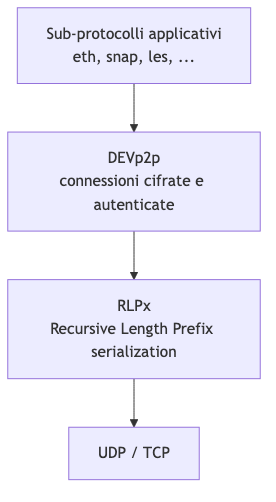
\includegraphics[keepaspectratio,alt={Diagramma Mermaid}]{images/mermaid-lezione-5-lab-p2p-networks-in-bitcoin-ed-ethereum-03.png}}
\emph{Fig. --- Lo stack tiered di Ethereum: RLPx fornisce
serializzazione e trasporto cifrato, DEVp2p gestisce le connessioni, e
diversi sub-protocolli usano lo stesso canale in multiplex.}

\begin{itemize}
\tightlist
\item
  \textbf{RLPx} (\emph{Recursive Length Prefix} serialization +
  crittografia) è il livello che rende possibile trovare peer e parlare
  con loro in modo sicuro. Definisce l'handshake iniziale e la
  serializzazione binaria dei messaggi.
\item
  \textbf{DEVp2p} è il protocollo che stabilisce e mantiene le
  connessioni persistenti su cui poi si parlano i sub-protocolli.
\item
  \textbf{Sub-protocolli} come \texttt{eth} (transazioni, blocchi,
  stato), \texttt{snap} (sync veloce), \texttt{les} (light client)
  viaggiano sulla stessa connessione DEVp2p in \textbf{multiplexing}.
\end{itemize}

\subsection{Node discovery in pratica}\label{node-discovery-in-pratica}

La scoperta dei peer avviene in due fasi distinte, sui due trasporti
diversi:

\textbf{Fase UDP (Kademlia)} --- localizzare peer:

\begin{enumerate}
\def\labelenumi{\arabic{enumi}.}
\tightlist
\item
  Il nodo chiede i ``vicini di se stesso'' a uno dei \textbf{bootnode}
  hardcoded (vedi \texttt{params/bootnodes.go} nel repository
  go-ethereum).
\item
  Ricevuta la lista iniziale, iterativamente invia \texttt{findnode} ai
  peer appena scoperti per riempire i bucket.
\item
  Si effettua un \textbf{bonding} via \texttt{ping/pong} per verificare
  che i peer siano vivi.
\end{enumerate}

\textbf{Fase TCP (RLPx + DEVp2p)} --- stabilire la comunicazione vera e
propria:

\begin{enumerate}
\def\labelenumi{\arabic{enumi}.}
\tightlist
\item
  \textbf{Handshake RLPx}: verifica versioni, stabilisce chiavi
  effimere, autentica la controparte. Documentazione ufficiale:
  \texttt{devp2p/rlpx.md\#initial-handshake}.
\item
  \textbf{Messaggio \texttt{Hello}} per comunicare le capability: quali
  sub-protocolli si è in grado di parlare. Da qui in poi il multiplexing
  è possibile.
\end{enumerate}

Importante: indipendentemente da quale sub-protocollo applicativo si
usi, è sempre RLPx a fornire il canale sottostante di autenticazione e
cifratura.

\pandocbounded{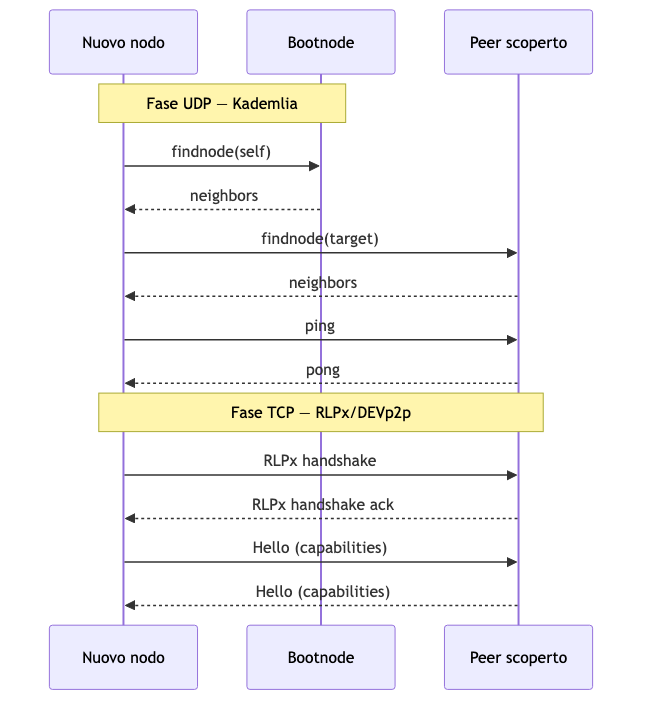
\includegraphics[keepaspectratio,alt={Diagramma Mermaid}]{images/mermaid-lezione-5-lab-p2p-networks-in-bitcoin-ed-ethereum-04.png}}
\emph{Fig. --- Le due fasi della scoperta e connessione in Ethereum: UDP
per trovare peer, TCP per parlarci in sicurezza.}

\subsection{Monitorare la rete
Ethereum}\label{monitorare-la-rete-ethereum}

Come per Bitcoin, anche Ethereum ha dashboard pubbliche.
\href{https://etherscan.io/nodetracker}{etherscan.io/nodetracker} è il
riferimento più usato per avere un quadro del numero di nodi attivi e
della loro distribuzione geografica.

\begin{center}\rule{0.5\linewidth}{0.5pt}\end{center}

\section{\texorpdfstring{Esempio pratico: connettersi con \texttt{geth}
a una rete
privata}{Esempio pratico: connettersi con geth a una rete privata}}\label{esempio-pratico-connettersi-con-geth-a-una-rete-privata}

La parte operativa del laboratorio mostra come usare \texttt{geth} (il
client Go di Ethereum) per entrare in una piccola rete privata,
bypassando o controllando il meccanismo di discovery.

\subsection{Opzioni rilevanti}\label{opzioni-rilevanti}

Due flag da ricordare:

\begin{itemize}
\tightlist
\item
  \texttt{-\/-bootnodes\ enode://...,enode://...} permette di
  specificare \emph{manualmente} la lista di bootnode invece di
  affidarsi a quelli hardcoded. Serve per reti private.
\item
  \texttt{-\/-nodiscover} disabilita del tutto la node discovery: utile
  quando si vuole una rete chiusa di nodi noti a priori.
\end{itemize}

\subsection{Procedura passo-passo}\label{procedura-passo-passo}

\begin{callouttip}{Avvio di un nodo su una rete privata}

\begin{enumerate}
\def\labelenumi{\arabic{enumi}.}
\item
  Installare \texttt{geth} seguendo la
  \href{https://geth.ethereum.org/docs/getting-started/installing-geth}{guida
  ufficiale}.
\item
  Creare una cartella di lavoro per i dati del nodo:

\begin{Shaded}
\begin{Highlighting}[]
\FunctionTok{mkdir}\NormalTok{ testLecture1}
\end{Highlighting}
\end{Shaded}
\item
  Procurarsi il file di genesi \texttt{testlecture1.json} (il
  significato dei suoi campi verrà discusso più avanti nel corso).
\item
  Inizializzare il datadir con il file di genesi:

\begin{Shaded}
\begin{Highlighting}[]
\ExtensionTok{geth} \AttributeTok{{-}{-}datadir}\NormalTok{ testLecture1/ init testlecture1.json}
\end{Highlighting}
\end{Shaded}
\item
  Avviare il nodo con una \texttt{networkid} custom e una porta
  dedicata, aprendo la console JavaScript interattiva:

\begin{Shaded}
\begin{Highlighting}[]
\ExtensionTok{geth} \AttributeTok{{-}{-}datadir}\NormalTok{ \textasciitilde{}/testLecture1/ }\AttributeTok{{-}{-}networkid}\NormalTok{ 35353 }\AttributeTok{{-}{-}port}\NormalTok{ 3333 }\AttributeTok{{-}{-}vmdebug}\NormalTok{ console}
\end{Highlighting}
\end{Shaded}
\end{enumerate}

\end{callouttip}

Una volta dentro la console si possono ispezionare e manipolare i peer:

\begin{itemize}
\tightlist
\item
  \texttt{admin.nodeInfo} --- stampa la propria \texttt{enode}, da
  condividere con altri per farsi trovare
\item
  \texttt{admin.peers} --- elenca i peer attualmente connessi
\item
  \texttt{admin.addPeer("enode://...")} --- aggiunge esplicitamente un
  peer di cui si conosce l'enode, senza passare dalla discovery
\end{itemize}

\begin{callouttip}{Reti private e --nodiscover}

In un laboratorio con pochi nodi conosciuti, disabilitare la discovery e
usare \texttt{admin.addPeer} è la strada più semplice per ottenere una
rete pulita, dove si ha controllo totale su chi parla con chi.
Riprodurre questo scenario è essenziale per poter osservare in maniera
deterministica il comportamento dei protocolli ai livelli superiori
(consenso, smart contract, \ldots).

\end{callouttip}

\begin{center}\rule{0.5\linewidth}{0.5pt}\end{center}

\section{Attacchi alla topologia di
Ethereum}\label{attacchi-alla-topologia-di-ethereum}

Il design di Kademlia è stato pensato per \textbf{scoraggiare} (non
impedire) la ricostruzione completa della routing table altrui. Due sono
le strategie che un avversario può tentare:

\begin{itemize}
\tightlist
\item
  \textbf{Usare il set noto degli ID esistenti}: invece di cercare ID
  casuali nello spazio a 512 bit (enorme), ci si concentra sugli ID dei
  peer effettivamente presenti nella rete. Questo riduce drasticamente
  lo spazio di ricerca.
\item
  \textbf{Brute force mirato}: poiché in pratica solo i bucket con
  prefisso corto comune sono popolati (gli altri sarebbero dedicati a
  ``distanze'' in cui statisticamente non c'è nessuno), si concentra lo
  sforzo lì.
\end{itemize}

La difesa principale --- lo \textbf{hash step} con Keccak-256 applicato
agli ID --- rende il costo della ricostruzione dipendente dal target e
non lineare: non basta fare 256 richieste \texttt{findnode}, bisogna
scegliere bene i target per coprire i bucket popolati.

\begin{calloutquestion}{Domanda aperta di ricerca}

Quando un nodo riceve un \texttt{findnode}, risponde con un messaggio
\texttt{neighbors} contenente i 16 nodi più vicini trovati nella propria
tabella. Quanti messaggi \texttt{findnode}, con quali target, sono
necessari per scaricare completamente la routing table di un nodo?

È una domanda non banale. I lavori di riferimento sono Henningsen et
al.~(\url{https://ieeexplore.ieee.org/document/8969695}) e Marcus et
al.~(\url{https://eprint.iacr.org/2018/236.pdf}), che analizzano eclipse
attack e ricostruzione di tabelle Kademlia in Ethereum.

\end{calloutquestion}

\begin{center}\rule{0.5\linewidth}{0.5pt}\end{center}

\section{Sintesi comparativa}\label{sintesi-comparativa}

\begin{calloutnote}{Bitcoin vs Ethereum al layer P2P}

Entrambe le reti rispondono allo stesso problema --- propagare
informazioni in una rete aperta senza conoscere la topologia globale ---
ma con filosofie opposte. \textbf{Bitcoin} privilegia la semplicità di
un gossip non strutturato: poche connessioni, propagazione randomizzata,
sicurezza di rete aggiunta solo tardivamente. \textbf{Ethereum} investe
in un overlay strutturato via Kademlia, con autenticazione e cifratura
by design, e uno stack tiered (RLPx / DEVp2p / sub-protocolli) che gli
permette di ospitare comodamente molti protocolli applicativi sulla
stessa infrastruttura. La differenza non è cosmetica: influenza la
resilienza agli attacchi di eclipse, la facilità di fingerprinting, e la
capacità di evolvere il protocollo aggiungendo nuovi sub-protocolli
senza rompere la rete.

\end{calloutnote}

\newpage

\chapter{Crittografia per P2P e
Blockchain}\label{crittografia-per-p2p-e-blockchain}

Due strumenti crittografici sono alla base di blockchain e DHT: le
\textbf{funzioni di hash} (collegano i blocchi rendendoli tamper-proof)
e le \textbf{firme digitali} (impediscono agli utenti di ripudiare le
proprie azioni). Strumenti più avanzati --- zero knowledge, strutture
dati autenticate, accumulatori crittografici --- verranno trattati più
avanti nel corso.

\begin{center}\rule{0.5\linewidth}{0.5pt}\end{center}

\section{Funzioni di Hash
Crittografiche}\label{funzioni-di-hash-crittografiche}

Una funzione di hash converte una stringa binaria di lunghezza
arbitraria (anche 0) in una stringa di lunghezza fissa. L'output ---
detto \emph{digest}, \emph{fingerprint} o informalmente \emph{checksum}
--- ha sempre la stessa dimensione indipendentemente dall'input (video,
audio, testo, eseguibili).

Per le strutture dati ordinarie, una funzione hash deve essere:
deterministica, efficiente da calcolare (es.
\texttt{y\ =\ x\ mod\ table\_dim}), pseudo-casuale per distribuire
uniformemente gli elementi, minimizzare le collisioni. Le funzioni hash
\textbf{crittografiche} aggiungono ulteriori proprietà di sicurezza.

\subsection{Proprietà Fondamentali}\label{proprietuxe0-fondamentali}

\textbf{Determinismo} --- La stessa funzione hash applicata più volte
allo stesso documento produce sempre lo stesso risultato.

\textbf{Fast Computation} --- L'hash deve essere computazionalmente
efficiente da calcolare.

\textbf{One-Way (Pre-image Resistance)} --- Dato un hash \(y\), deve
essere computazionalmente impossibile trovare un \(x\) tale che
\(H(x) = y\). Con SHA-1 (160 bit) un attacco brute-force richiederebbe
\(2^{71}\) anni.

\textbf{Avalanche Effect} --- Un singolo bit di differenza nell'input
produce un hash completamente diverso; cambiare anche solo 1 bit
modifica tutto l'output.

\textbf{Collision Resistance} --- Le collisioni esistono matematicamente
(per il \emph{Pigeonhole Principle}: con più input che output, almeno un
output deve corrispondere a più di un input), ma devono essere
computazionalmente impossibili da costruire intenzionalmente.

\begin{callouttip}{Pigeonhole Principle}

Se si scelgono 51 numeri interi tra 1 e 100, almeno due devono essere
consecutivi. Dimostrazione: le ``buche'' sono le coppie \{1,2\},
\{3,4\}, \ldots, \{99,100\} --- 50 coppie per 51 numeri. Per il
principio del piccione, almeno una buca contiene due piccioni.

\end{callouttip}

\textbf{Weak Collision Resistance (Second Pre-image Resistance)} ---
Dato un input \(x\) noto, deve essere difficile trovare un \(x' \neq x\)
tale che \(H(x') = H(x)\). Questo previene, ad esempio, la distribuzione
di software corrotto spacciato per autentico: un attaccante non può
generare un file malevolo con lo stesso hash del software legittimo.

\subsection{Il Paradosso del Compleanno e la Sicurezza
Effettiva}\label{il-paradosso-del-compleanno-e-la-sicurezza-effettiva}

Per trovare una collisione in modo garantito bastano \(2^n + 1\) input
distinti (per Pigeonhole). Tuttavia il \textbf{Birthday Paradox} abbassa
drasticamente il limite pratico:

In una stanza di \(n\) persone scelte a caso, \(n = 23\) è sufficiente
perché la probabilità che due condividano il compleanno superi il 50\%.
Questo perché la seconda persona deve evitare 1 compleanno su 365, la
terza 2 su 365, ecc.; il prodotto delle probabilità di ``nessuna
collisione'' scende rapidamente. Formalmente, con
\(\sqrt{2^n} = 2^{n/2}\) input casuali si ha già alta probabilità di
collisione.

Per una funzione hash con \(n\)-bit di output, bastano
\(\approx 2^{n/2}\) input casuali per trovare una collisione con
probabilità 0,5. La sicurezza effettiva è quindi \textbf{metà dei bit di
output}.

\begin{calloutwarning}{Quantificazione brute force}

Se un computer calcola 10.000 hash/sec, calcolare \(2^{128}\) hash
richiederebbe \(10^{27}\) anni. Anche se tutti i computer mai costruiti
dall'umanità avessero calcolato sin dall'inizio dell'universo, la
probabilità di aver trovato una collisione sarebbe infinitesimamente
piccola.

\end{calloutwarning}

{\def\LTcaptype{none} % do not increment counter
\begin{longtable}[]{@{}llll@{}}
\toprule\noalign{}
Algoritmo & Bit output & Sicurezza effettiva & Stato \\
\midrule\noalign{}
\endhead
\bottomrule\noalign{}
\endlastfoot
MD2, MD4 & 128 bit & 64 bit & Ritirati --- vulnerabili \\
MD5 & 128 bit & 64 bit & Vulnerabile (ok per app non di sicurezza) \\
SHA-1 & 160 bit & 80 bit & Ritirato --- debole \\
SHA-256 & 256 bit & 128 bit & Usato da Bitcoin --- sicuro \\
SHA-512 & 512 bit & 256 bit & Corrente --- massima sicurezza \\
\end{longtable}
}

Almeno \textbf{80 bit} di sicurezza sono necessari. Le funzioni hash
hanno storicamente una vita utile di circa \textbf{10 anni}. Lo standard
attuale è \textbf{SHA-3} (Keccak), adottato anche da Ethereum.

\begin{calloutwarning}{Hash non crittografici}

La \textbf{parità a blocco a 8 bit}: è banale trovare una collisione
invertendo un numero pari di bit nella stessa colonna. Il \textbf{CRC}
(Cyclic Redundancy Check) è il resto di una divisione polinomiale lunga
--- ottimo per rilevare burst error nelle comunicazioni, ma facile da
collidere intenzionalmente. CRC è stato usato erroneamente nel
protocollo \textbf{WEP} (Wired Equivalent Privacy) dove si richiedeva
integrità crittografica.

\end{calloutwarning}

\subsection{Cryptanalysis}\label{cryptanalysis}

Oltre al brute force, la \textbf{crittoanalisi} cerca debolezze logiche
nell'algoritmo: scorciatoie, buchi nella funzione. Una funzione si dice
\emph{broken} quando è possibile trovare collisioni significativamente
più velocemente del brute force.

\subsection{Proprietà Avanzate}\label{proprietuxe0-avanzate}

\textbf{Hiding} --- Dato \(H(R \| x)\), deve essere impossibile ricavare
informazioni su \(x\). Formalmente: \(H\) è \emph{hiding} se, scelto
\(R\) da una distribuzione con alta min-entropy (nessun valore più
probabile degli altri), dato \(H(R \| x)\) è computazionalmente
impossibile trovare \(x\).

Le funzioni base non garantiscono hiding se lo spazio di input è piccolo
e prevedibile (es. password), rendendole vulnerabili ai \textbf{Rainbow
Table Attack}: si pre-calcolano le hash di tutte le password possibili
in una tabella; al login si cerca il hash nel database. La soluzione è
concatenare un valore casuale \(R\) a 256 bit ad alta min-entropy:
\(H(R \| x)\), rendendo lo spazio di ricerca enorme.

\textbf{Puzzle-Friendliness} --- Per qualsiasi output target \(y\) e
valore casuale \(k\) ad alta min-entropy, trovare \(x\) tale che
\(H(k \| x) = y\) richiede un attacco esaustivo in tempo
\(\approx 2^n\), senza scorciatoie algoritmiche. Questa proprietà
implica che nessuna strategia di risoluzione è significativamente
migliore della ricerca esaustiva.

\begin{center}\rule{0.5\linewidth}{0.5pt}\end{center}

\section{Applicazioni delle Funzioni di
Hash}\label{applicazioni-delle-funzioni-di-hash}

\subsection{Applicazioni
non-blockchain}\label{applicazioni-non-blockchain}

\textbf{Gestione password} --- I sistemi memorizzano
\(H(\text{password})\) invece del testo in chiaro. Anche in caso di
compromissione del database, le password originali non sono
recuperabili.

\textbf{Integrity checks (anti-tampering)} --- Si calcolano checksum per
i file da scaricare o trasmettere. Prima di aprire o eseguire un file,
si calcola il suo hash e lo si confronta con il checksum atteso: se
coincidono, il file non è stato alterato o corrotto.

\textbf{Data deduplication} --- Se due file hanno lo stesso hash, sono
identici --- senza dover confrontare i file interi. Usato ad esempio da
\textbf{eMule} con MD5 per verificare che due file siano identici anche
se descritti da keyword diverse.

\textbf{DHT} --- Le chiavi vengono hashate per localizzare il nodo
responsabile in modo efficiente e deterministico.

\subsection{Applicazioni blockchain}\label{applicazioni-blockchain}

\textbf{Hash Pointers} --- Un hash pointer è sia un riferimento a una
posizione (dove si trova il dato) sia un hash crittografico del dato in
quella posizione. Permette di verificare che i dati non siano stati
alterati. Bitcoin usa una \textbf{hash chain} (blockchain) per
memorizzare il ledger delle transazioni: ogni blocco contiene l'hash del
blocco precedente, garantendo la \emph{tamper-freeness} --- modificare
un blocco invalida tutti i successivi.

\pandocbounded{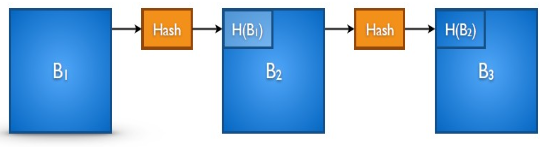
\includegraphics[keepaspectratio]{images/Pasted-image-20260407111722.png}}

\textbf{Commitment Scheme} --- Permette di ``chiudere in una busta'' una
decisione senza terze parti fidate.

\textbf{Hash Puzzles (Proof of Work)} --- Trovare \(x\) tale che
\(H(r \| x) \in S\).

\begin{center}\rule{0.5\linewidth}{0.5pt}\end{center}

\section{Commitment Scheme}\label{commitment-scheme}

\subsection{Motivazione: Sasso-Carta-Forbici
online}\label{motivazione-sasso-carta-forbici-online}

Alice e Bob giocano a sasso-carta-forbici via Internet senza terze parti
fidate. Il problema: chi va per primo perde, perché l'avversario può
adattarsi. La soluzione è che chi va per primo \emph{si impegna} a una
scelta senza rivelarla.

Il flusso con commitment crittografico (\(R_A\) = valore casuale scelto
da Alice):

\[A \to B: h_A = H(R_A \| \text{paper})\] \[B \to A: \text{scissors}\]
\[A \to B: R_A, \text{paper}\]

Bob verifica che \(h_A = H(R_A \| \text{paper})\). Se sì, sa che Alice
non ha barato.

\begin{itemize}
\tightlist
\item
  Bob non riesce a determinare la scelta di Alice perché non conosce
  \(R_A\) (\emph{hiding} + \emph{pre-image resistance})
\item
  Alice non può cambiare idea dopo aver ricevuto ``scissors'': dovrebbe
  trovare \(R'_A\) tale che
  \(H(R_A \| \text{paper}) = H(R'_A \| \text{stone})\) → violazione
  della \textbf{second-preimage resistance}
\end{itemize}

La proprietà per cui il mittente non può cambiare il valore impegnato si
chiama \textbf{binding}.

\subsection{API e Implementazione}\label{api-e-implementazione}

\begin{verbatim}
com   ← commit(value, nonce)     // sigilla il valore
                                 // pubblica com
match ← verify(com, nonce, value) // apre la busta
\end{verbatim}

Implementazione con funzione hash: - \texttt{commit(msg,\ nonce)} =
\(H(\text{msg} \| \text{nonce})\) - \texttt{verify(com,\ nonce,\ msg)} =
\((H(\text{msg} \| \text{nonce}) == \text{com})\)

L'uso del \texttt{nonce} (number used once) garantisce la proprietà
hiding anche quando lo spazio dei messaggi è piccolo.

\begin{center}\rule{0.5\linewidth}{0.5pt}\end{center}

\section{Search Puzzle (Proof of
Work)}\label{search-puzzle-proof-of-work}

Un search puzzle consiste in: una funzione hash crittografica \(H\), un
valore casuale \(r\), un insieme target \(S\). La soluzione è un valore
\(x\) tale che:

\[H(r \| x) \in S\]

Si tratta di un \textbf{partial pre-image attack}: si deve trovare parte
dell'input affinché l'output appartenga a un insieme (non a un singolo
valore come nella pre-image resistance). La difficoltà si modula
definendo la dimensione di \(S\): un \(S\) più grande rende il puzzle
più facile. In \textbf{Bitcoin}, \(S\) è definito dal numero di zeri
iniziali richiesti nell'hash SHA-256 del blocco.

La puzzle-friendliness garantisce che non esistano scorciatoie: l'unico
metodo è il tentativo esaustivo.

\begin{center}\rule{0.5\linewidth}{0.5pt}\end{center}

\section{Crittografia Asimmetrica e Firme
Digitali}\label{crittografia-asimmetrica-e-firme-digitali}

La crittografia asimmetrica usa una coppia di chiavi: una \textbf{chiave
privata} (\(K^-\)), nota solo al proprietario, e una \textbf{chiave
pubblica} (\(K^+\)), derivata matematicamente da essa ma non
invertibile. La proprietà fondamentale è la \textbf{reciprocità}: ciò
che una chiave cifra, l'altra decifra, e viceversa.

\textbf{Cifratura (riservatezza)} --- Alice cifra un messaggio con la
chiave \emph{pubblica} di Bob; solo Bob, con la sua chiave
\emph{privata}, può decifrarlo.

\textbf{Vantaggi rispetto alla crittografia simmetrica}: nessun bisogno
di concordare preventivamente una chiave condivisa. Chi vuole ricevere
messaggi cifrati deve solo rendere pubblica la propria chiave pubblica.
Finché la chiave privata è tenuta segreta, nessun altro può decifrare.

\subsection{Firme Digitali}\label{firme-digitali}

\begin{calloutdefinition}{Firma Digitale}

Meccanismo equivalente a una firma autografa ma molto più sicuro.
Fornisce tre garanzie: \textbf{autenticazione} (il messaggio è stato
creato dal mittente riconosciuto), \textbf{non ripudio} (il mittente non
può negare di aver firmato --- la firma può essere portata in tribunale
come prova), \textbf{integrità} (il messaggio non è stato alterato
durante la trasmissione).

\end{calloutdefinition}

Il flusso è l'\textbf{inverso della cifratura}: il mittente firma con la
propria chiave \emph{privata}, chiunque può verificare con la chiave
\emph{pubblica}.

\textbf{Firma naive}: Bob firma \(m\) cifrando con la sua chiave privata
\(K^-_B\), creando \(K^-_B(m)\). Invia ad Alice la coppia
\((m, K^-_B(m))\). Alice verifica applicando la chiave pubblica:
\(K^+_B(K^-_B(m)) = m\). Se coincide, sa che solo Bob --- possessore di
\(K^-_B\) --- ha potuto firmare.

Poiché firmare asimmetricamente un messaggio lungo è computazionalmente
costoso, in pratica si firma solo il \textbf{digest}:

\[\text{firma} = K^-_B(H(m))\]

Il verificatore calcola \(H(m)\) e lo confronta con
\(K^+_B(\text{firma})\): se coincidono, l'autenticità è garantita.

Per avere simultaneamente \textbf{riservatezza + integrità}: il mittente
firma con la propria chiave privata e cifra il pacchetto completo con la
chiave pubblica del destinatario. Il destinatario decifra con la propria
chiave privata e verifica con la chiave pubblica del mittente.

\subsection{API Standard}\label{api-standard}

\begin{verbatim}
(sk, pk) := generateKeys(keysize)    // sk = signing key, pk = public key
sig      := sign(sk, message)        // cifra con sk → firma
isValid  := verify(pk, message, sig) // decifra sig con pk, confronta con message
\end{verbatim}

Proprietà richiesta:
\texttt{verify(pk,\ message,\ sign(sk,\ message))\ ==\ true}.

\textbf{Sfida principale}: cosa impedisce a un avversario di imparare a
firmare messaggi analizzando la chiave pubblica? Le costruzioni basate
su problemi hard (fattorizzazione, logaritmo discreto) rendono questo
computazionalmente impossibile.

{\def\LTcaptype{none} % do not increment counter
\begin{longtable}[]{@{}
  >{\raggedright\arraybackslash}p{(\linewidth - 4\tabcolsep) * \real{0.3333}}
  >{\raggedright\arraybackslash}p{(\linewidth - 4\tabcolsep) * \real{0.3333}}
  >{\raggedright\arraybackslash}p{(\linewidth - 4\tabcolsep) * \real{0.3333}}@{}}
\toprule\noalign{}
\begin{minipage}[b]{\linewidth}\raggedright
Algoritmo
\end{minipage} & \begin{minipage}[b]{\linewidth}\raggedright
Base matematica
\end{minipage} & \begin{minipage}[b]{\linewidth}\raggedright
Note
\end{minipage} \\
\midrule\noalign{}
\endhead
\bottomrule\noalign{}
\endlastfoot
RSA & Fattorizzazione di numeri primi (one-way trapdoor function) &
Standard storico \\
DSA & Logaritmo discreto & Standard NIST \\
ECDSA & Logaritmo discreto su curve ellittiche & Usato da Bitcoin \\
\end{longtable}
}

\textbf{Bitcoin e ECDSA}: ogni transazione Bitcoin contiene in input una
firma e una chiave pubblica; in output il codice (script) per la
procedura di verifica.

\subsection{Certification Authorities}\label{certification-authorities}

La debolezza degli schemi asimmetrici è la \textbf{weak authentication}:
verificare la firma garantisce solo che chi ha firmato possiede la
chiave privata corrispondente --- non che sia davvero chi afferma di
essere.

\begin{callouttip}{Pizza Prank}

Alice crea un ordine di pizze a nome di Bob, lo firma con la
\emph{propria} chiave privata, e invia alla pizzeria la propria chiave
pubblica spacciandola per quella di Bob. La pizzeria verifica la firma
(correttamente), consegna le pizze a Bob. La weak authentication non
basta.

\end{callouttip}

Le \textbf{Certification Authority (CA)} risolvono il problema: emettono
certificati digitali che legano crittograficamente un'identità alla sua
chiave pubblica, firmando essi stessi il certificato con la propria
chiave privata (di cui tutti si fidano).

\begin{center}\rule{0.5\linewidth}{0.5pt}\end{center}

\section{Hash vs Cifratura}\label{hash-vs-cifratura}

\begin{calloutnote}{Differenza concettuale}

La \textbf{cifratura} è bidirezionale: con la chiave giusta si cifra e
si decifra. L'\textbf{hashing} è irreversibile per definizione: non
esiste un'operazione di ``de-hashing''. Sono strumenti complementari,
non intercambiabili.

\end{calloutnote}

\begin{center}\rule{0.5\linewidth}{0.5pt}\end{center}

\section{RIPEMD-160 e Bitcoin}\label{ripemd-160-e-bitcoin}

Bitcoin usa \textbf{due} funzioni hash: SHA-256 per il Proof of Work e
\textbf{RIPEMD-160} (160 bit, output) per la derivazione degli indirizzi
wallet. Il doppio hash \texttt{RIPEMD160(SHA256(pubkey))} produce
l'indirizzo Bitcoin a partire dalla chiave pubblica.

\newpage

\chapter{Strutture Dati per DHT e
Blockchain}\label{strutture-dati-per-dht-e-blockchain}

Questa lezione copre quattro strutture dati fondamentali per sistemi
distribuiti e blockchain: \textbf{Hash Pointer}, \textbf{Filtri di
Bloom}, \textbf{Merkle Tree} e \textbf{Merkle Patricia Trie}.

\begin{center}\rule{0.5\linewidth}{0.5pt}\end{center}

\section{Hash Pointer}\label{hash-pointer}

\begin{calloutdefinition}{Hash Pointer}

Un puntatore tradizionale indica \emph{dove} si trova un dato. Un hash
pointer indica \emph{dove} si trova il dato \textbf{e} ne contiene
l'hash crittografico, permettendo di verificare che non sia stato
alterato. È un puntatore \emph{tamper-evident}.

\end{calloutdefinition}

L'idea è costruire strutture dati concatenando componenti tramite hash
pointer invece di puntatori normali. Per calcolare l'hash pointer a un
blocco, si fa l'hash dell'intero blocco \textbf{incluso} il suo hash
pointer al blocco precedente.

L'esempio più noto è la \textbf{blockchain}: ogni blocco contiene l'hash
pointer al blocco precedente. Modificare il blocco \(k\) invalida il suo
hash, quindi non coincide con il puntatore nel blocco \(k+1\). In una
blockchain \textbf{Proof of Work}, ogni blocco contiene anche la prova
che il PoW è stato eseguito con successo: modificare i dati richiede di
rieseguire il PoW per tutti i blocchi successivi --- computazionalmente
impossibile.

Gli hash pointer funzionano su qualsiasi struttura senza cicli: liste,
alberi, DAG. Applicazioni: - \textbf{Bitcoin/Ethereum}: catena di
blocchi con SHA-256 e RIPEMD-160 (doppio hash) - \textbf{IPFS}: Merkle
DAG - \textbf{eMule} (\emph{Advanced Intelligent Corruption Handling}):
prima applicazione storica; verifica che i blocchi di un file scaricato
dalla rete non siano stati manomessi, sfruttando i Merkle Tree

\begin{center}\rule{0.5\linewidth}{0.5pt}\end{center}

\section{Filtri di Bloom}\label{filtri-di-bloom}

\subsection{Il Problema}\label{il-problema}

Dato un insieme \(S = \{s_1, s_2, \ldots, s_n\}\) con \(n\) molto
grande, vogliamo rispondere alla domanda ``l'elemento \(k\) appartiene a
\(S\)?'' usando poca memoria. Memorizzare tutti gli elementi
esplicitamente è proibitivo. La soluzione è un'approssimazione: si
accetta un trade-off tra spazio occupato e probabilità di falsi
positivi.

\begin{calloutdefinition}{Filtro di Bloom}

Struttura dati probabilistica per membership query. Può rispondere: -
``\(k\) \textbf{non} appartiene a \(S\)'' → \textbf{garantito} (nessun
falso negativo) - ``\(k\) \textbf{forse} appartiene a \(S\)'' → con una
certa probabilità di falso positivo

\end{calloutdefinition}

\subsection{Costruzione}\label{costruzione}

Un filtro di Bloom è un vettore \(B[1 \ldots m]\) di \(m\) bit
(inizialmente tutti a 0) e \(k\) funzioni di hash \(h_1, \ldots, h_k\),
indipendenti e uniformemente distribuite, ciascuna mappante in
\([1, m]\). Non è necessario che siano crittografiche: bastano funzioni
veloci. Esempio: \(h_i(x) = MD5(x \| i)\).

\textbf{Inserimento} di un elemento \(x \in S\): si calcolano
\(h_1(x), \ldots, h_k(x)\) e si impostano a 1 i bit corrispondenti. Un
bit può essere target di più di un elemento.

\textbf{Lookup} di un elemento \(y\): si calcolano
\(h_1(y), \ldots, h_k(y)\). - Se \textbf{tutti} i bit corrispondenti
sono 1 → \(y\) è \emph{probabilmente} in \(S\) - Se \textbf{anche uno
solo} è 0 → \(y\) è \emph{certamente} assente

I falsi positivi accadono quando tutti i bit di un elemento estraneo
sono già stati impostati a 1 da altri elementi.

\subsection{Probabilità di Falso
Positivo}\label{probabilituxe0-di-falso-positivo}

L'analisi si può modellare col paradigma \textbf{balls and bins}:
inserire \(n\) elementi con \(k\) funzioni equivale a lanciare \(kn\)
palline in \(m\) secchi.

Con \(n\) elementi inseriti, la probabilità che un bit specifico sia
ancora a 0 è:

\[p' = \left(1 - \frac{1}{m}\right)^{kn} \approx e^{-kn/m}\]

La probabilità di un falso positivo (tutti i \(k\) bit a 1 per un
elemento assente) è:

\[P_{fp} = \left(1 - e^{-kn/m}\right)^k\]

Questa dipende da due parametri: - \textbf{\(m/n\)} (bit per elemento):
per \(k\) fisso, al crescere di \(m\) la \(P_{fp}\) \textbf{decresce
esponenzialmente} - \textbf{\(k\)} (numero di funzioni di hash): fissato
\(m/n\), la \(P_{fp}\) prima decresce poi \textbf{risale} all'aumentare
di \(k\). Con pochi bit per elemento (es. \(m/n = 2\)) troppe funzioni
riempiono il filtro di 1 e peggiorano il risultato; con \(m/n = 10\)
aumentare \(k\) diminuisce sempre la \(P_{fp}\)

\begin{callouttip}{Regola pratica}

Il filtro diventa efficace quando \(m = c \cdot n\) con \(c\) costante.
Con \(m = 8n\) (8 bit per elemento) e \(k \approx 5\text{–}6\) funzioni,
la probabilità di falso positivo è circa \(2\%\) --- buon compromesso
con un numero limitato di bit.

\end{callouttip}

\subsection{Operazioni sugli Insiemi}\label{operazioni-sugli-insiemi}

{\def\LTcaptype{none} % do not increment counter
\begin{longtable}[]{@{}
  >{\raggedright\arraybackslash}p{(\linewidth - 4\tabcolsep) * \real{0.3333}}
  >{\raggedright\arraybackslash}p{(\linewidth - 4\tabcolsep) * \real{0.3333}}
  >{\raggedright\arraybackslash}p{(\linewidth - 4\tabcolsep) * \real{0.3333}}@{}}
\toprule\noalign{}
\begin{minipage}[b]{\linewidth}\raggedright
Operazione
\end{minipage} & \begin{minipage}[b]{\linewidth}\raggedright
Metodo
\end{minipage} & \begin{minipage}[b]{\linewidth}\raggedright
Note
\end{minipage} \\
\midrule\noalign{}
\endhead
\bottomrule\noalign{}
\endlastfoot
Unione \(S_1 \cup S_2\) & OR bit a bit di \(B_1\) e \(B_2\) & Esatto
(stessi \(m\) e \(k\)) \\
Intersezione \(S_1 \cap S_2\) & AND bit a bit di \(B_1\) e \(B_2\) &
Approssimato --- un bit a 1 in entrambi può venire da elementi diversi
non nell'intersezione \\
Cancellazione & Non supportata & Azzerare un bit rimuoverebbe anche
altri elementi che lo condividono \\
\end{longtable}
}

Per supportare la cancellazione si usano i \textbf{Counting Bloom
Filter}: ogni entry è un contatore invece di un bit. L'inserimento
incrementa, la cancellazione decrementa.

\subsection{Applicazioni Reali}\label{applicazioni-reali}

{\def\LTcaptype{none} % do not increment counter
\begin{longtable}[]{@{}
  >{\raggedright\arraybackslash}p{(\linewidth - 2\tabcolsep) * \real{0.5000}}
  >{\raggedright\arraybackslash}p{(\linewidth - 2\tabcolsep) * \real{0.5000}}@{}}
\toprule\noalign{}
\begin{minipage}[b]{\linewidth}\raggedright
Sistema
\end{minipage} & \begin{minipage}[b]{\linewidth}\raggedright
Uso
\end{minipage} \\
\midrule\noalign{}
\endhead
\bottomrule\noalign{}
\endlastfoot
\textbf{Bitcoin (SPV client)} & I client mobili costruiscono un filtro
con gli indirizzi di interesse e lo inviano a un nodo completo
(bandwidth saving + privacy). Il nodo filtra le transazioni rilevanti
senza trasmettere l'intera blockchain \\
\textbf{Ethereum} & I \emph{log bloom} negli header dei blocchi
riassumono gli eventi degli smart contract. Esempio: trovare tutti i
token venduti da un utente in un blocco di 500 transazioni --- si
interroga il log bloom per la presenza dell'utente e si analizza il
blocco solo in caso di match, evitando il parsing sequenziale \\
\textbf{Google Chrome} & Filtro locale per verificare se un URL è in un
database di siti malevoli, prima di fare una query remota al server \\
\textbf{Google BigTable} & Evita costosi disk lookup cercando prima nel
filtro, aumentando le performance delle query al database \\
\end{longtable}
}

\begin{center}\rule{0.5\linewidth}{0.5pt}\end{center}

\section{Merkle Tree}\label{merkle-tree}

\subsection{Il Problema dell'Authenticated File
Storage}\label{il-problema-dellauthenticated-file-storage}

Alice salva un file \(F\) (contenuto \(D\)) su un server remoto e
cancella la copia locale. Quando lo recupera, come verifica che il
server non abbia restituito un file alterato \(D' \neq D\)?

\begin{itemize}
\tightlist
\item
  \textbf{Soluzione 1} (banale): non cancellare \(D\) --- inutile se
  manca la memoria
\item
  \textbf{Soluzione 2} (hash singolo): Alice conserva \(H(D)\); verifica
  confrontando \(H(D') = H(D)\). Funziona per il file intero, ma se
  Alice vuole solo un frammento deve scaricare tutto e ricalcolare
  l'hash
\item
  \textbf{Soluzione 3} (Merkle Tree): aggiungere struttura al commitment
  --- non un singolo hash ma una gerarchia di hash
\end{itemize}

\begin{calloutdefinition}{Merkle Tree}

Struttura dati introdotta da \textbf{Ralph Merkle nel 1979} per
sintetizzare grandi quantità di dati con verifica efficiente. È un
albero binario completo di hash costruito da un insieme iniziale
\(\{x_1, \ldots, x_n\}\) (con \(n\) potenza di 2): - Le \textbf{foglie}
contengono l'hash di ciascun dato: \(y_i = H(x_i)\) - I \textbf{nodi
interni} contengono l'hash della concatenazione dei figli:
\(H(\text{figlio\_sx} \| \text{figlio\_dx})\) - La \textbf{radice}
(\textbf{Merkle Root Hash}) riassume crittograficamente l'intero dataset

\end{calloutdefinition}

\subsection{Costruzione}\label{costruzione-1}

Con \(n\) dati \(x_1, x_2, \ldots, x_n\) e funzione hash \(H\): - Ogni
nodo interno memorizza
\(H(x \| y) = H(\text{concatenazione dei figli})\) - Il commitment
finale è il Merkle Root \(y_{2n-1}\) - \textbf{Costo di costruzione}:
\(O(n)\) spazio e \(O(n)\) hash

\pandocbounded{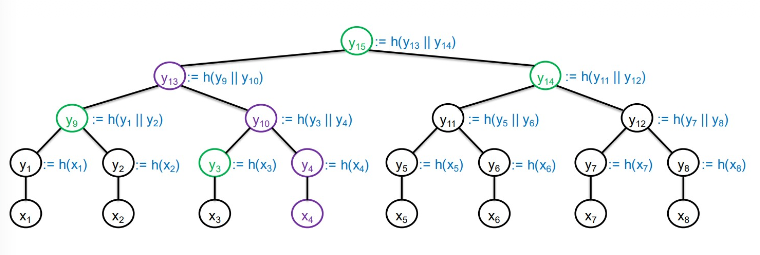
\includegraphics[keepaspectratio]{images/Pasted-image-20260407112004.png}}
\#\#\# Merkle Proof (Proof of Inclusion)

Protocollo file storage: 1. Alice invia \(D\) al server; il server
memorizza \((F, D)\) 2. Alice calcola il \textbf{Merkle Tree Root} (MTR)
da \(D\), conserva MTR (\(O(1)\) --- 256 bit), cancella \(D\) 3. Più
tardi: Alice chiede al server il chunk \(x_i\) 4. Il server (Prover)
restituisce \(x_i\) + \textbf{prova di inclusione} \(p\) (gli hash dei
fratelli lungo il percorso foglia→radice) 5. Alice (Verifier) verifica
\(p\) rispetto al MTR conservato

\begin{callouttip}{Merkle Proof Concreta}

Per dimostrare che \(D = x_4\) appartiene all'albero, si esibiscono i
fratelli lungo il percorso: \(y_3\), \(y_9\), \(y_{14}\).

La verifica ricalcola: - \(z_4 = H(D)\) - \(z_{10} = H(y_3 \| z_4)\) -
\(z_{13} = H(y_9 \| z_{10})\) - \(z_{15} = H(z_{13} \| y_{14})\)

Si controlla che \(z_{15} = y_{15}\) (la radice fidata). Se sì, il chunk
è autentico.

\end{callouttip}

{\def\LTcaptype{none} % do not increment counter
\begin{longtable}[]{@{}
  >{\raggedright\arraybackslash}p{(\linewidth - 2\tabcolsep) * \real{0.5000}}
  >{\raggedright\arraybackslash}p{(\linewidth - 2\tabcolsep) * \real{0.5000}}@{}}
\toprule\noalign{}
\begin{minipage}[b]{\linewidth}\raggedright
Proprietà
\end{minipage} & \begin{minipage}[b]{\linewidth}\raggedright
Valore
\end{minipage} \\
\midrule\noalign{}
\endhead
\bottomrule\noalign{}
\endlastfoot
Costo costruzione & \(O(n)\) spazio e hash \\
Spazio commitment & \(O(1)\) --- solo il Merkle Root (256 bit) \\
Dimensione prova & \(O(\log n)\) hash \\
Costo di verifica & \(O(\log n)\) operazioni \\
Falsi negativi & Impossibili --- se \(x_i \in \{x_1,\ldots,x_n\}\) la
prova è sempre costruibile \\
Falsi positivi & Impossibili --- una prova falsa richiederebbe trovare
una collisione hash \\
\end{longtable}
}

\subsection{Proof of Non-Membership}\label{proof-of-non-membership}

Per dimostrare che \(\text{Data} \notin \{x_1, \ldots, x_n\}\): si
ordinano le foglie e si trovano \(x_i < \text{Data} < x_{i+1}\); si
dimostrano le inclusioni di \(x_i\) e \(x_{i+1}\).

\subsection{Applicazioni}\label{applicazioni-1}

\begin{itemize}
\tightlist
\item
  \textbf{Bitcoin}: memorizza le transazioni in ogni blocco
\item
  \textbf{Ethereum}: usa Merkle-Patricia Tries per stato e transazioni
\item
  \textbf{IPFS}: Merkle DAG
\item
  \textbf{Apache Cassandra}: verifica dell'integrità dei dati replicati
\end{itemize}

\begin{center}\rule{0.5\linewidth}{0.5pt}\end{center}

\section{Trie, Patricia Trie e Merkle Patricia
Trie}\label{trie-patricia-trie-e-merkle-patricia-trie}

\subsection{Trie (Prefix Tree / Radix
Tree)}\label{trie-prefix-tree-radix-tree}

Il nome \emph{trie} viene da ``retrieval''. È una struttura ad albero
per stringhe in cui ogni arco è etichettato con un carattere (o lettera
dell'alfabeto); un percorso dalla radice a un nodo \emph{marcato} forma
una stringa valida. Con l'alfabeto inglese ogni nodo può avere fino a 26
figli.

\textbf{Ricerca}: si scende dall'alto seguendo i caratteri della
stringa; se si trova il percorso e il nodo finale è marcato → successo;
se si è bloccati o il nodo finale è non marcato → fallimento.

\textbf{Problema}: la maggior parte dei nodi ha un solo figlio, creando
lunghe catene inutili (es. ``Ann'', ``Anna'', ``Annab'', ``Annabe'',
``Annabel'' formano un percorso senza biforcazioni). Lo spazio richiesto
è elevato.

\subsection{Patricia Trie}\label{patricia-trie}

\textbf{PATRICIA} = \emph{Practical Algorithm To Retrieve Information
Coded In Alphanumeric} (1960). È una versione compressa del trie: le
catene di nodi a figlio unico vengono \textbf{compresse in un singolo
arco} con etichetta multipla (la concatenazione delle etichette dei nodi
compressi). Il risultato è un albero in cui ogni nodo interno ha
\textbf{almeno due figli}.

Il Patricia Trie funziona anche come \textbf{dizionario di coppie
(chiave, valore)}: le chiavi sono le stringhe rappresentate nell'albero,
i valori sono memorizzati nei nodi terminali. Usato in Ethereum per lo
stato dei contratti.

\subsection{Nibble}\label{nibble}

In Ethereum le chiavi sono stringhe esadecimali suddivise in
\textbf{nibble} (mezzo byte = 4 bit = 1 carattere esadecimale). Questo
permette una condivisione più \textbf{granulare} dei prefissi: 16
possibili direzioni per ogni nodo interno (anziché 256 per i byte
interi).

\subsection{Merkle Patricia Trie
(Ethereum)}\label{merkle-patricia-trie-ethereum}

\begin{calloutdefinition}{Merkle Patricia Trie}

Struttura ibrida introdotta nel \textbf{Yellow Paper di Ethereum} e ora
usata nella maggior parte delle blockchain EVM-based. Combina: - La
\textbf{compressione dei prefissi} del Patricia Trie → ricerca veloce e
deterministica - La \textbf{garanzia crittografica} dei Merkle Tree →
integrità e tamper-proof validation

Usata da Ethereum per memorizzare lo stato degli account/contratti e le
transazioni.

\end{calloutdefinition}

Le coppie (chiave, valore) in Ethereum possono essere: -
\texttt{(indirizzo\ account\ →\ saldo)} -
\texttt{(identificatore\ transazione\ →\ importo\ trasferito)}

I nodi del Merkle Patricia Trie sono di tre tipi:

{\def\LTcaptype{none} % do not increment counter
\begin{longtable}[]{@{}
  >{\raggedright\arraybackslash}p{(\linewidth - 4\tabcolsep) * \real{0.3333}}
  >{\raggedright\arraybackslash}p{(\linewidth - 4\tabcolsep) * \real{0.3333}}
  >{\raggedright\arraybackslash}p{(\linewidth - 4\tabcolsep) * \real{0.3333}}@{}}
\toprule\noalign{}
\begin{minipage}[b]{\linewidth}\raggedright
Tipo
\end{minipage} & \begin{minipage}[b]{\linewidth}\raggedright
Contenuto
\end{minipage} & \begin{minipage}[b]{\linewidth}\raggedright
Ruolo
\end{minipage} \\
\midrule\noalign{}
\endhead
\bottomrule\noalign{}
\endlastfoot
\textbf{Leaf node} & Nibble finali della chiave + valore & Nodo
terminale; memorizza il valore \\
\textbf{Extension node} (shared node) & Nibble condivisi (prefisso
comune) + hash pointer al branch node & Compressione del prefisso
comune \\
\textbf{Branch node} & Array di 16 elementi (uno per nibble 0--F) +
eventuale valore & Punto di biforcazione tra prefissi \\
\end{longtable}
}

\begin{callouttip}{Costruzione MPT}

Inserzione di `do' → creazione di un nodo foglia. Inserzione di `puppy'
→ il prefisso comune (in esadecimale `646f') genera uno shared node +
branch node; la nuova foglia viene collegata tramite un \textbf{hash
pointer} (l'hash del nodo foglia stesso) → questa è la componente
\emph{Merkle} dell'albero. Il nibble `6' è condiviso tra tutti i
prefissi → viene creato un nodo dedicato al livello di nibble.

\end{callouttip}

Un singolo hash pointer alla radice del MPT garantisce l'integrità
crittografica dell'intero stato di Ethereum: qualunque modifica cambia
la radice.

\begin{center}\rule{0.5\linewidth}{0.5pt}\end{center}

\section{Riepilogo}\label{riepilogo}

{\def\LTcaptype{none} % do not increment counter
\begin{longtable}[]{@{}
  >{\raggedright\arraybackslash}p{(\linewidth - 6\tabcolsep) * \real{0.2500}}
  >{\raggedright\arraybackslash}p{(\linewidth - 6\tabcolsep) * \real{0.2500}}
  >{\raggedright\arraybackslash}p{(\linewidth - 6\tabcolsep) * \real{0.2500}}
  >{\raggedright\arraybackslash}p{(\linewidth - 6\tabcolsep) * \real{0.2500}}@{}}
\toprule\noalign{}
\begin{minipage}[b]{\linewidth}\raggedright
Struttura
\end{minipage} & \begin{minipage}[b]{\linewidth}\raggedright
Problema risolto
\end{minipage} & \begin{minipage}[b]{\linewidth}\raggedright
Complessità
\end{minipage} & \begin{minipage}[b]{\linewidth}\raggedright
Garanzie
\end{minipage} \\
\midrule\noalign{}
\endhead
\bottomrule\noalign{}
\endlastfoot
\textbf{Hash Pointer} & Tamper-evidence su strutture concatenate &
\(O(1)\) per verifica & Qualunque manomissione è rilevabile \\
\textbf{Filtro di Bloom} & Membership query su insiemi enormi & \(O(k)\)
insert/lookup & No falsi negativi; falsi positivi controllabili con
\(m/n\) e \(k\) \\
\textbf{Merkle Tree} & Autenticazione di frammenti di dati & \(O(n)\)
costruzione, \(O(\log n)\) prova/verifica & Nessun falso positivo né
negativo \\
\textbf{Merkle Patricia Trie} & Stato globale distribuito e verificabile
& \(O(\log n)\) lookup & Integrità crittografica + ricerca efficiente
per prefisso \\
\end{longtable}
}

\newpage

\chapter{Introduzione alla
Blockchain}\label{introduzione-alla-blockchain}

\section{Il Ledger Distribuito}\label{il-ledger-distribuito}

\begin{calloutdefinition}{Ledger}

Un registro cronologico di eventi, \textbf{append-only}: si possono solo
aggiungere voci, mai modificare o cancellare quelle passate. Funziona
come un notaio digitale: tutti i partecipanti devono concordare sul suo
contenuto.

\end{calloutdefinition}

Un ledger non serve solo per le transazioni finanziarie: qualunque
applicazione che necessita di un log di eventi può beneficiarne. Un
ledger distribuito viene replicato tra i nodi di una rete P2P: ogni nodo
possiede la stessa copia immutabile.

\begin{callouttip}{Alice come intermediaria}

Alice gestisce un'azienda che fa da intermediaria tra dettaglianti e
grossisti. Ha difficoltà a mantenere un ledger consistente perché serve
centinaia di clienti. Decide di condividere il ledger con tutti:
ciascuno mantiene una copia e la aggiorna. Emerge immediatamente il
problema della \textbf{consistenza}: chi decide cosa è scritto nel
ledger?

\end{callouttip}

Quando il ledger è organizzato come una sequenza di blocchi concatenati
prende il nome di \textbf{blockchain}. Esistono architetture alternative
--- \textbf{IOTA}, ad esempio, usa un DAG invece di una catena lineare.

Ogni blocco contiene tre elementi: - \textbf{Dati} --- le transazioni
(es. ``Alice invia X a Bob'') - \textbf{Hash del blocco} --- impronta
crittografica del contenuto - \textbf{Hash del blocco precedente} --- il
collegamento che forma la catena (hash pointer)

La catena parte dal \textbf{Genesis Block}. Modificare un blocco cambia
il suo hash, invalidando tutti i successivi. In una blockchain
\textbf{Proof of Work}, ripristinarli non richiede solo ricalcolare gli
hash: bisogna trovare un valore che, combinato con il nuovo hash,
risolva il PoW per ogni blocco successivo. Questo è computazionalmente
impossibile. Altre blockchain possono usare meccanismi diversi (es.
PoS).

\begin{center}\rule{0.5\linewidth}{0.5pt}\end{center}

\section{Il Problema del Consenso}\label{il-problema-del-consenso}

In un sistema distribuito senza autorità centrale, chi decide quale
operazione aggiungere al registro?

\begin{calloutdefinition}{Consenso}

Accordo tra i nodi di una rete distribuita sull'\textbf{ordine e la
validità} delle informazioni memorizzate su un ledger condiviso e
replicato. Il consenso è il meccanismo che definisce: chi decide quale
operazione viene aggiunta alla blockchain, e quale tra le operazioni da
confermare viene scelta.

\end{calloutdefinition}

Il consenso è essenziale per prevenire il \textbf{double spending}: le
informazioni digitali si copiano facilmente --- i bit sono più facili da
copiare della carta --- quindi senza un accordo collettivo nulla
impedisce di spendere la stessa moneta due volte. Se la maggioranza è
onesta, i nodi dovrebbero votare contro le transazioni di double
spending.

Un approccio classico è il \textbf{consenso basato sul voto}: ogni
operazione viene trasmessa in broadcast sulla rete e si raccolgono i
voti; la maggioranza determina la correttezza delle transazioni e
l'ordine dei blocchi.

In un mondo ideale funzionerebbe, ma in reti P2P aperte ci sono due
ostacoli reali: - Ritardi e partizioni di rete (\emph{jitter}, nodi che
non si vedono temporaneamente) - Nodi malintenzionati (\textbf{byzantine
parties}) che possono comportarsi in modo arbitrario

\begin{center}\rule{0.5\linewidth}{0.5pt}\end{center}

\section{L'Attacco Sybil}\label{lattacco-sybil}

Il punto debole del consenso a voto in reti aperte: cosa significa
``maggioranza'' se chiunque può creare identità false?

\begin{calloutdefinition}{Attacco Sybil}

Un attaccante inietta nella rete un numero arbitrario di identità
fittizie per ottenere la maggioranza dei voti e manipolare il consenso.
Il nome viene dalle Sibille dell'antica Grecia --- profetesse attraverso
cui parlava una divinità, metafora di più identità per la stessa
persona; rappresentate nel pavimento del \textbf{Duomo di Siena}. In
informatica il libro di riferimento è \emph{Sybil} (Flora Rheta
Schreiber, 1973), su una donna con 16 personalità distinte.

\end{calloutdefinition}

Iniettare identità false è banale: basta registrarsi molte volte con la
stessa DHT. Il singolo nodo impersona così molteplici identità logiche.

\textbf{Obiettivi dell'attacco Sybil:} - Routing attacks (controllare i
percorsi di instradamento) - Controllare la replica dei dati -
Disturbare la connettività della rete - Essere la maggioranza nel voto →
consenso nelle criptovalute

\textbf{Difese:} - \textbf{Proof of Work} (Bitcoin, Ethereum): richiede
potere computazionale - \textbf{Proof of Stake}: richiede stake
economico - \textbf{Certified Node-IDs}: richiede un'autorità centrale
--- non è una soluzione P2P

\subsection{Double Spending con Sybil}\label{double-spending-con-sybil}

Alice esegue un attacco Sybil assumendo più del 50\% delle identità
nella rete. Poi tenta di spendere lo stesso bitcoin sia verso Bob che
verso Charlie. Usando le sue identità multiple (\textgreater50\%),
approva con il consenso entrambe le transazioni di double spending →
l'attacco ha successo.

\begin{center}\rule{0.5\linewidth}{0.5pt}\end{center}

\section{La Proof of Work}\label{la-proof-of-work}

\textbf{La soluzione di Bitcoin}: invece di contare le identità, si
conta la \textbf{potenza di calcolo}.

\begin{calloutdefinition}{Proof of Work}

Per partecipare al consenso, un nodo deve risolvere un problema
computazionalmente difficile ma facile da verificare. Creare identità
multiple è inutile se si ha un solo computer: per manipolare la rete
bisogna controllare la maggioranza della potenza di calcolo globale. Gli
attacchi Sybil diventano costosi e inutili.

\end{calloutdefinition}

La PoW funziona come una \textbf{lotteria} in cui i biglietti sono molto
costosi (risolvere il problema). Il vincitore della lotteria decide
\textbf{unilateralmente} quale sarà il prossimo blocco e riceve una
ricompensa economica per comportarsi onestamente --- incentivo a seguire
le regole.

\begin{center}\rule{0.5\linewidth}{0.5pt}\end{center}

\section{Proof of Ownership e UTXO}\label{proof-of-ownership-e-utxo}

Oltre al consenso, serve dimostrare la \textbf{proprietà} degli asset.

\begin{callouttip}{ICO di Alice}

Alice vuole aprire un ristorante ma l'affitto è alto e i venture
capitalist sono avidi. Usa una \textbf{ICO} (\emph{Initial Coin
Offering}): propone un progetto su blockchain, raccoglie finanziamenti,
crea \textbf{token} come compensazione per i finanziatori --- nel caso
concreto, \emph{cryptocoupon} per pasti scontati all'apertura del
ristorante.

Alice usa un ledger per registrare i trasferimenti di token. Il
problema: come può un finanziatore dimostrare di possedere un coupon?
Come può Alice dimostrare di essere autorizzata a emetterlo? Senza una
CA centralizzata.

\end{callouttip}

La soluzione è puramente crittografica: Alice genera una coppia
\texttt{(chiave\ pubblica,\ chiave\ privata)}. Chiunque conosca la
chiave privata corrispondente alla chiave pubblica di Alice possiede i
suoi cryptocoupon --- Alice stessa, chiunque lei voglia (a cui cede la
chiave privata), o chiunque la rubi.

\begin{itemize}
\tightlist
\item
  \textbf{Chiave pubblica} → identifica il proprietario del token
\item
  \textbf{Chiave privata} → conferisce il possesso effettivo e autorizza
  i trasferimenti tramite firma digitale
\end{itemize}

\subsection{Esempio di Spesa}\label{esempio-di-spesa}

Alice (con chiave privata \texttt{af876f536...}) vuole trasferire il
50\% di un coupon a ciascuno di due finanziatori: 1. Identifica le
chiavi pubbliche dei destinatari (es. \texttt{1FE1W2EEJE...},
\texttt{A5d65ab38...}) 2. Firma il trasferimento con la propria chiave
privata → dimostra di essere autorizzata 3. Registra la transazione
firmata sul ledger 4. I due destinatari usano le proprie chiavi private
per riscuotere il mezzo coupon

\begin{calloutwarning}{La chiave privata è tutto}

Chiunque ottenga la chiave privata di un utente ha il pieno controllo
dei suoi asset --- non esiste recupero, non esiste banca che possa
aiutare.

\end{calloutwarning}

\subsection{UTXO}\label{utxo}

Bitcoin non ha il concetto di ``conto'' con saldo. Esistono solo
trasferimenti. Per sapere quanto possiede, un utente scorre l'intero
registro cercando gli \textbf{UTXO} (\emph{Unspent Transaction Output}):
le transazioni ricevute e non ancora spese. Spendere un UTXO lo
distrugge e ne crea di nuovi per il destinatario (e per il resto).

\begin{center}\rule{0.5\linewidth}{0.5pt}\end{center}

\section{Permissionless vs
Permissioned}\label{permissionless-vs-permissioned}

{\def\LTcaptype{none} % do not increment counter
\begin{longtable}[]{@{}
  >{\raggedright\arraybackslash}p{(\linewidth - 4\tabcolsep) * \real{0.3333}}
  >{\raggedright\arraybackslash}p{(\linewidth - 4\tabcolsep) * \real{0.3333}}
  >{\raggedright\arraybackslash}p{(\linewidth - 4\tabcolsep) * \real{0.3333}}@{}}
\toprule\noalign{}
\begin{minipage}[b]{\linewidth}\raggedright
\end{minipage} & \begin{minipage}[b]{\linewidth}\raggedright
Permissionless
\end{minipage} & \begin{minipage}[b]{\linewidth}\raggedright
Permissioned
\end{minipage} \\
\midrule\noalign{}
\endhead
\bottomrule\noalign{}
\endlastfoot
\textbf{Accesso} & Aperto a chiunque & Limitato a nodi autorizzati \\
\textbf{Identità} & Anonima/pseudonima & Certificata (umani con
password/chiavi, sensori con chiavi) \\
\textbf{Consenso} & PoW, PoS (costoso ma senza fiducia) & PBFT e simili
(efficiente, ambiente controllato) \\
\textbf{Esempi} & Bitcoin, Ethereum, Steemit, Algorand & Hyperledger,
Ethereum Quorum, Corda \\
\textbf{Rischi} & Fork, attacchi (es. DAO hack da \$54M) & Richiede
fiducia negli operatori \\
\end{longtable}
}

\subsection{Permissionless}\label{permissionless}

Chiunque può partecipare e minare. Il sistema funziona senza fidarsi di
nessuno, grazie agli incentivi economici. Non richiede autorità
centrale.

\subsection{Permissioned}\label{permissioned}

Accesso e consenso limitati a partecipanti con identità verificata. Le
differenze chiave rispetto alle permissionless sono: - Le parti hanno
\textbf{identità}: umani con password/chiavi, sensori con chiavi proprie
--- tutti \textbf{autenticati} - Si usano meccanismi di consenso
diversi, basati sul voto tra nodi noti - \textbf{Accountability}: se un
nodo viene scoperto a barare, è identificabile --- diverso approccio
agli attacchi Sybil

\begin{callouttip}{Supply chain del frozen yogurt}

Alice vende il ristorante e apre un'attività di frozen yogurt. Le
spedizioni arrivano sciolte: di chi è la colpa --- Bob (il
trasportatore) o Carol (la fabbrica)? Con una blockchain permissioned
accessibile solo a Bob, Carol e sensori di temperatura certificati, ogni
evento è tracciato e firmato digitalmente. La responsabilità è
attribuibile con certezza.

\end{callouttip}

Il \textbf{PBFT} (\emph{Practical Byzantine Fault Tolerance}, Castro e
Liskov, 1999) è il protocollo di consenso tipico delle blockchain
permissioned: tolera comportamenti arbitrari di nodi malevoli in reti
asincrone, con prestazioni nettamente superiori alla PoW in ambienti con
partecipanti noti e controllati.

\newpage

\chapter{Bitcoin}\label{bitcoin}

\begin{calloutwarning}{Bitcoin è difficile da capire}

Bitcoin si trova al crocevia di più discipline: non solo informatica, ma
economia, diritto, politica e scienze sociali. Non è solo una tecnologia
--- è un cambio di paradigma culturale con implicazioni legali,
politiche e sociali rilevanti.

\end{calloutwarning}

\begin{center}\rule{0.5\linewidth}{0.5pt}\end{center}

\section{Le Origini: dalla Moneta Elettronica a
Bitcoin}\label{le-origini-dalla-moneta-elettronica-a-bitcoin}

L'idea di una moneta elettronica (\textbf{e-cash}) è nata molto prima di
Bitcoin. Già nel 1999 Milton Friedman prevedeva lo sviluppo di un metodo
per trasferire fondi su Internet tra due sconosciuti --- esattamente
come scambiarsi una banconota da 20 dollari.

Il primo tentativo concreto fu quello di David Chaum, professore a
Berkeley e ``padrino'' del movimento cyberpunk, negli anni Ottanta. Il
suo sistema si basava sulle \textbf{firme cieche} (\emph{blind
signatures}):

\begin{enumerate}
\def\labelenumi{\arabic{enumi}.}
\tightlist
\item
  L'utente genera una moneta: un token casuale unico
\item
  L'utente ``acceca'' (\emph{blinds}) il token e lo invia alla banca per
  la firma
\item
  La banca firma il token accecato senza poterne vedere il contenuto ---
  al momento della firma, sa di aver firmato una moneta, ma non quale
\item
  L'utente ``scopre'' (\emph{unblinds}) la moneta, ottenendo un token
  firmato e valido che può spendere anonimamente
\end{enumerate}

Il sistema garantiva l'\textbf{intracciabilità} (\emph{pecunia non
olet}), ma non risolveva completamente il double spending: l'utente
poteva inviare lo stesso token a due commercianti diversi. La
contromisura era che ogni commerciante, al momento della riscossione,
sottoponeva la moneta alla banca per verifica: se la moneta era già
stata spesa, la transazione veniva rifiutata. Elegante --- ma richiedeva
ancora la fiducia in una banca centrale.

\begin{calloutdefinition}{Requisiti della Moneta Elettronica}

L'e-cash deve conservare gli attributi fisici del contante: -
\textbf{Non falsificabile} (\emph{unforgeable}): impossibile il double
spending - \textbf{Non tracciabile} (\emph{untraceable}): la privacy
dell'utente deve essere garantita --- \emph{pecunia non olet}

\end{calloutdefinition}

La storia dei pagamenti ha attraversato millenni: dai bilanci
mesopotamici (2040 a.C.), alle banche centralizzate (BNP Paribas, 1848),
ai circuiti VISA (1958), fino all'eCash di Chaum (1983). Il vero salto
verso il \emph{decentralized banking} arriva nel 2008, seguito da
Ethereum (2015) e Zcash (2016).

\begin{center}\rule{0.5\linewidth}{0.5pt}\end{center}

\section{Satoshi Nakamoto e il
Whitepaper}\label{satoshi-nakamoto-e-il-whitepaper}

Nell'ottobre 2008, sotto lo pseudonimo \textbf{Satoshi Nakamoto}, viene
pubblicato \emph{``Bitcoin: A Peer-to-Peer Electronic Cash System''}
sulla mailing list di crittografia. La proposta: pagamenti online
diretti tra due parti, senza istituzioni finanziarie. Le firme digitali
da sole non bastano --- dipendere da terze parti fiduciarie per evitare
il double spending ne annulla i benefici.

\begin{callouttip}{L’Annuncio Originale}

Il messaggio di Nakamoto alla mailing list il 31 ottobre 2008:

\emph{``I've been working on a new electronic cash system that's fully
peer-to-peer, with no trusted third party. The main properties:
Double-spending is prevented with a peer-to-peer network. No mint or
other trusted parties. Participants can be anonymous. New coins are made
from Hashcash style proof-of-work. The proof-of-work for new coin
generation also powers the network to prevent double-spending.''}

\end{callouttip}

La soluzione di Bitcoin è una rete P2P che marca temporalmente le
transazioni inserendole in una catena basata su \textbf{Proof of Work}.
La catena più lunga è sia la prova dell'ordine cronologico degli eventi,
sia la garanzia che quella sequenza provenga dalla maggioranza della
potenza computazionale.

\subsection{Nakamoto Timeline}\label{nakamoto-timeline}

{\def\LTcaptype{none} % do not increment counter
\begin{longtable}[]{@{}
  >{\raggedright\arraybackslash}p{(\linewidth - 2\tabcolsep) * \real{0.5000}}
  >{\raggedright\arraybackslash}p{(\linewidth - 2\tabcolsep) * \real{0.5000}}@{}}
\toprule\noalign{}
\begin{minipage}[b]{\linewidth}\raggedright
Data
\end{minipage} & \begin{minipage}[b]{\linewidth}\raggedright
Evento
\end{minipage} \\
\midrule\noalign{}
\endhead
\bottomrule\noalign{}
\endlastfoot
2008-08-18 & Registrazione del dominio bitcoin.org \\
2008-10-31 & Pubblicazione del Bitcoin paper \\
2008-11-09 & Progetto Bitcoin registrato su sourceforge.net \\
2009-01-03 & Genesis Block minato alle 18:15:05 GMT \\
2009-01-09 & Bitcoin v0.1 rilasciato e annunciato sulla mailing list di
crittografia \\
2009-01-12 & Prima transazione (blocco 170) da Satoshi a Hal Finney \\
2010 (metà) & Nakamoto interrompe ogni interazione e lascia il progetto
alla comunità \\
\end{longtable}
}

\begin{callouttip}{La Pizza da 10.000 BTC}

Nel maggio 2010, sul forum Bitcointalk, Laszlo Hanyecz offrì 10.000 BTC
(circa 25 dollari all'epoca, ricevuti come ricompensa di mining) a
chiunque gli consegnasse ``un paio di pizze''. La richiesta fu esaudita
da un ragazzo della costa ovest: primo acquisto documentato di beni
reali con Bitcoin.

\end{callouttip}

\subsection{Bitcoin: Protocollo e
Valuta}\label{bitcoin-protocollo-e-valuta}

È importante distinguere tra due accezioni del termine:

\begin{itemize}
\tightlist
\item
  \textbf{Bitcoin} (maiuscolo): il protocollo, il software e la comunità
\item
  \textbf{bitcoin} (minuscolo): le unità della valuta, gli \emph{asset}
  nativi intrinseci al protocollo
\end{itemize}

I bitcoin vengono trasferiti usando il protocollo Bitcoin. Non esiste
bitcoin al di fuori del protocollo che lo definisce.

\begin{center}\rule{0.5\linewidth}{0.5pt}\end{center}

\section{Caratteristiche e
Resilienza}\label{caratteristiche-e-resilienza}

Bitcoin è pensato come alternativa ai sistemi di pagamento tradizionali.
Il confronto con le soluzioni precedenti è diretto:

{\def\LTcaptype{none} % do not increment counter
\begin{longtable}[]{@{}
  >{\raggedright\arraybackslash}p{(\linewidth - 2\tabcolsep) * \real{0.5000}}
  >{\raggedright\arraybackslash}p{(\linewidth - 2\tabcolsep) * \real{0.5000}}@{}}
\toprule\noalign{}
\begin{minipage}[b]{\linewidth}\raggedright
Problema dei sistemi precedenti
\end{minipage} & \begin{minipage}[b]{\linewidth}\raggedright
Soluzione Bitcoin
\end{minipage} \\
\midrule\noalign{}
\endhead
\bottomrule\noalign{}
\endlastfoot
Serve un server fidato o istituzione finanziaria & \textbf{Apertura}:
basta un client Bitcoin, senza conto bancario né carta di credito;
nessun ente centralizzato controlla l'offerta di moneta \\
Nessuna anonimità & \textbf{Pseudo-anonimità}: transazioni senza
disclosure dell'identità; gli indirizzi come pseudonimi --- come
``pagare in contanti'' \\
Alte commissioni di transazione & Commissioni minime (almeno nei primi
anni; PayPal richiede 2--10\%) \\
\end{longtable}
}

Bitcoin è transnazionale e senza confini (\emph{borderless}),
\textbf{permissionless} (nessun regolatore centrale), \textbf{censorship
resistant} (i fondi non possono essere congelati),
\textbf{cross-jurisdictional} (nessuna giurisdizione specifica si
applica) e pseudonima. L'infrastruttura opera su sospetto di default:
nessun partecipante deve fidarsi degli altri.

\subsection{Perché Bitcoin è
Sopravvissuto}\label{perchuxe9-bitcoin-uxe8-sopravvissuto}

In 17 anni, Bitcoin ha dimostrato una resilienza notevole. Ha superato:

\begin{itemize}
\tightlist
\item
  Il collasso di \textbf{Mt. Gox} nel 2014 (Magic the Gathering Online
  eXchange): all'epoca era il più grande exchange USD/Bitcoin al mondo;
  a febbraio 2014 dichiarò bancarotta, con circa 850.000 BTC (\$450
  milioni all'epoca) scomparsi --- probabilmente a causa di un attacco
  di \textbf{malleabilità} del protocollo (trattato nelle lezioni
  successive)
\item
  L'associazione con il dark web attraverso \textbf{Silk Road}: mercato
  online operante come Tor hidden service, attivo tra febbraio 2011 e
  ottobre 2013, usato per acquistare beni illeciti (droghe, materiale
  pornografico) anonimamente; il gestore Ross William Ulbricht è stato
  condannato all'ergastolo
\item
  Attacchi ransomware come \textbf{WannaCry}
\end{itemize}

Nonostante le enormi fluttuazioni di prezzo e lo scetticismo di
economisti come Paul Krugman e Alan Greenspan --- che lo hanno
paragonato a uno schema Ponzi --- il sistema è rimasto vitale.

\subsection{Ragioni del Successo}\label{ragioni-del-successo}

Il successo si spiega con diversi fattori:

\begin{itemize}
\tightlist
\item
  \textbf{Ragioni ideologiche}: criptoanarchia (nessuno controlla la
  moneta), movimento cyberpunk
\item
  \textbf{Tempismo}: nato durante la crisi finanziaria del 2008 ---
  impossibile ``stampare'' nuovi BTC arbitrariamente
\item
  \textbf{Bitcoin come oro digitale}: offerta controllata dal
  protocollo, nessun intervento sull'offerta monetaria, sicuro ---
  alcuni suggeriscono di investire fino al 5\% del portafoglio in
  Bitcoin
\item
  \textbf{Presenza di exchange}: piattaforme dove i bitcoin si scambiano
  con valute fiat tradizionali. Dopo Mt. Gox (chiuso nel 2014), ne sono
  nati altri più affidabili: CoinDesk, BPI, Bitstamp, Bitfinex,
  Coinbase, itBit, OKCoin
\item
  \textbf{Mercati regolamentati}: stanno emergendo mercati Bitcoin con
  supervisione legale
\item
  \textbf{Ecosistema in espansione}: centinaia di altre criptovalute e
  token nati negli ultimi anni
\end{itemize}

\begin{center}\rule{0.5\linewidth}{0.5pt}\end{center}

\section{Identità e Indirizzi}\label{identituxe0-e-indirizzi}

In assenza di una Certification Authority, Bitcoin gestisce le identità
tramite crittografia asimmetrica con l'algoritmo \textbf{ECDSA}
(\emph{Elliptic Curve Digital Signature Algorithm}) sulla curva
\emph{secp256k1}:

\[y^2 = x^3 + ax + b \pmod{p}\]

La derivazione di un indirizzo parte dalla chiave privata e procede in
un'unica direzione:

\[sk \xrightarrow{\text{curva ellittica}} pk \xrightarrow{\text{SHA-256}} \xrightarrow{\text{RIPEMD-160}} \xrightarrow{\text{Base58}} \text{Indirizzo Bitcoin}\]

La \textbf{chiave privata} (\texttt{sk}) deve rimanere segreta:
controlla i fondi associati. La \textbf{chiave pubblica} (\texttt{pk})
si deriva da \texttt{sk} tramite moltiplicazione sulla curva ellittica
--- operazione irreversibile. La chiave pubblica funziona come il ``nome
pubblico'' dell'utente e ``parla per'' la sua identità; in pratica, si
usa più spesso \texttt{Hash(pk)} --- l'indirizzo. Se una transazione
reca una firma \texttt{sig} tale che
\texttt{verify(pk,\ data,\ sig)\ ==\ true}, si può ragionevolmente
concludere che \texttt{pk} ha autorizzato quella transazione.

L'\textbf{indirizzo} è l'hash della chiave pubblica, codificato in
\textbf{Base58}: un alfabeto alfanumerico da cui Nakamoto ha rimosso i
caratteri ambigui (\texttt{0}, \texttt{O}, \texttt{I}, \texttt{l}) per
prevenire errori di trascrizione. Base58 usa 58 caratteri (62
dell'alfabeto alfanumerico completo meno i 4 ambigui): permette di
rappresentare grandi numeri in formato compatto.

\begin{calloutnote}{Nessuna cifratura}

In Bitcoin non esiste nulla di cifrato per nascondere informazioni ---
tutto è pubblico sulla blockchain. Le chiavi servono solo a dimostrare,
tramite firma digitale, la proprietà e l'autorizzazione a spendere.

Per garantire privacy si possono utilizzare tecniche di \textbf{Zero
Knowledge} --- ma non sono native nel protocollo base.

\end{calloutnote}

\begin{calloutnote}{Gli Indirizzi Possono Rappresentare Script}

Nella maggior parte dei casi un indirizzo Bitcoin corrisponde all'hash
di una coppia di chiavi pubblica/privata. Tuttavia, un indirizzo può
anche rappresentare uno \textbf{script} (P2SH --- Pay-to-Script-Hash).
Chiunque può generare nuove identità in qualsiasi momento e quante ne
vuole. Gli indirizzi funzionano come il nome del beneficiario in un
assegno: \emph{``pay to the order of xxx''}. Per quanto riguarda la
privacy: gli indirizzi non sono direttamente collegati all'identità
reale, ma un osservatore può correlare l'attività di un indirizzo nel
tempo e trarre inferenze --- quindi si parla di
\textbf{pseudo-anonimità}.

\end{calloutnote}

\begin{center}\rule{0.5\linewidth}{0.5pt}\end{center}

\section{Flusso di Pagamento}\label{flusso-di-pagamento}

Il flusso tipico di un pagamento Bitcoin segue quattro passi:

\begin{enumerate}
\def\labelenumi{\arabic{enumi}.}
\tightlist
\item
  Il commerciante Bob comunica il proprio indirizzo \textbf{fuori banda}
  (\emph{out of band}) ad Alice --- non attraverso la rete P2P Bitcoin.
  L'indirizzo può essere condiviso via QR code, email, o verbalmente
\item
  Alice genera una transazione che paga all'indirizzo di Bob e la
  trasmette in \textbf{broadcast} sulla rete P2P
\item
  I miner raccolgono le transazioni trasmesse in un blocco candidato;
  uno dei blocchi candidati contenente la transazione viene minato
\item
  Bob attende le \textbf{conferme} sulla transazione prima di consegnare
  i beni
\end{enumerate}

\begin{center}\rule{0.5\linewidth}{0.5pt}\end{center}

\section{Il Modello UTXO}\label{il-modello-utxo}

Bitcoin non ha il concetto di ``conto'' con un saldo. Il sistema si basa
sugli \textbf{UTXO} (\emph{Unspent Transaction Output}): il saldo
mostrato da un wallet è la somma di tutti gli UTXO associati agli
indirizzi dell'utente, calcolata scorrendo la blockchain e aggregando
tutti gli output non spesi.

\begin{callouttip}{Lo Stato di Bitcoin}

``Lo stato di Bitcoin risiede negli output non spesi delle
transazioni.'' --- L'insieme degli UTXO rappresenta lo spazio condiviso
dell'intera rete Bitcoin. A differenza di Ethereum (che richiede una
rappresentazione di stato più complessa), il modello UTXO è semplice e
verificabile. L'UTXO set è molto più piccolo dell'intera blockchain e
può essere mantenuto in RAM, velocizzando i controlli di validità.

\end{callouttip}

Le transazioni distruggono UTXO esistenti (input) e ne creano di nuovi
(output). I bitcoin di un utente possono essere distribuiti come UTXO
tra centinaia di transazioni e centinaia di blocchi --- non esiste una
nozione di saldo memorizzato su un indirizzo:

\[\sum \text{inputs} \geq \sum \text{outputs}\]

La differenza è la \textbf{transaction fee}, che spetta al minatore che
include la transazione nel blocco:

\[fee = \sum \text{inputs} - \sum \text{outputs}\]

Gli input devono essere consumati per intero --- non si può frazionare
un UTXO alla fonte. Per questo le transazioni comuni hanno due output:
uno per il destinatario e uno di ``resto'' (\emph{change}) verso un
indirizzo del mittente.

Le strutture di transazione più comuni:

{\def\LTcaptype{none} % do not increment counter
\begin{longtable}[]{@{}
  >{\raggedright\arraybackslash}p{(\linewidth - 6\tabcolsep) * \real{0.2500}}
  >{\raggedright\arraybackslash}p{(\linewidth - 6\tabcolsep) * \real{0.2500}}
  >{\raggedright\arraybackslash}p{(\linewidth - 6\tabcolsep) * \real{0.2500}}
  >{\raggedright\arraybackslash}p{(\linewidth - 6\tabcolsep) * \real{0.2500}}@{}}
\toprule\noalign{}
\begin{minipage}[b]{\linewidth}\raggedright
Tipo
\end{minipage} & \begin{minipage}[b]{\linewidth}\raggedright
Input
\end{minipage} & \begin{minipage}[b]{\linewidth}\raggedright
Output
\end{minipage} & \begin{minipage}[b]{\linewidth}\raggedright
Uso tipico
\end{minipage} \\
\midrule\noalign{}
\endhead
\bottomrule\noalign{}
\endlastfoot
\textbf{Comune} & 1 & 2 & Pagamento + resto al mittente \\
\textbf{Aggregazione} & N & 1 & Unire micro-UTXO in uno solo
(equivalente di cambiare un mucchio di monete con una banconota); può
essere target di \textbf{dusting attack} \\
\textbf{Distribuzione} & 1 & N & Pagare più destinatari (es.
stipendi) \\
\end{longtable}
}

L'aggregazione viene anche sfruttata per \textbf{transazioni
multi-firma} (\emph{multisignature}): più parti contribuiscono input e
firmano congiuntamente.

\begin{center}\rule{0.5\linewidth}{0.5pt}\end{center}

\section{La Struttura JSON di una
Transazione}\label{la-struttura-json-di-una-transazione}

Una transazione Bitcoin reale è rappresentata in formato JSON con tre
sezioni principali:

\textbf{Metadati:} - \texttt{hash}: hash dell'intera transazione ---
identificatore univoco - \texttt{version}: permette interpretazioni
diverse di alcuni campi - \texttt{locktime}: definisce il momento più
precoce in cui la transazione può essere aggiunta alla blockchain;
impostato a zero nella maggior parte delle transazioni per indicare
esecuzione immediata; usato in transazioni di escrow e nel Lightning
Network (canale di pagamento)

\textbf{Input} --- array JSON dove ogni elemento contiene: - Hash
pointer alla transazione precedente + indice dell'output da spendere -
Script di sblocco (\emph{unlocking script})

\textbf{Output} --- array JSON dove ogni elemento contiene: - Valore da
trasferire in quell'output (in satoshi) - Script di blocco
(\emph{locking script}) contenente l'indirizzo del destinatario

\begin{center}\rule{0.5\linewidth}{0.5pt}\end{center}

\section{Il Linguaggio di Scripting}\label{il-linguaggio-di-scripting}

Ogni UTXO è governato da uno \textbf{script}: un programma che definisce
le condizioni per spenderlo. La validazione concatena uno
\emph{scriptSig} (script di sblocco, fornito da chi spende) con uno
\emph{scriptPubKey} (script di blocco, imposto da chi ha creato l'UTXO)
e li esegue insieme.

Il linguaggio di scripting di Bitcoin è deliberatamente:

\begin{itemize}
\tightlist
\item
  \textbf{Non Turing-completo} --- nessun loop, per impedire cicli
  infiniti che bloccherebbero i nodi in fase di validazione; tutti i
  full node (miner e nodi completi, non mobile) devono validare gli
  script
\item
  \textbf{Stateless} --- tutta l'informazione necessaria all'esecuzione
  è contenuta nello script stesso; nessuno stato persiste tra esecuzioni
  (a differenza di Ethereum)
\item
  \textbf{Deterministico} --- l'esecuzione è sempre identica su
  qualsiasi hardware
\item
  \textbf{Semplice e compatto} --- opcode da un byte (256 istruzioni
  possibili); istruzione di base: aritmetica, logica
  (\texttt{IF...THEN...ELSE}), istruzioni speciali per crittografia
  (hash, verifica firma, verifica multi-firma)
\end{itemize}

L'esecuzione è \textbf{stack-based} (simile al linguaggio FORTH): le
istruzioni operano su una pila.

Gli opcode principali:

{\def\LTcaptype{none} % do not increment counter
\begin{longtable}[]{@{}
  >{\raggedright\arraybackslash}p{(\linewidth - 4\tabcolsep) * \real{0.3333}}
  >{\raggedright\arraybackslash}p{(\linewidth - 4\tabcolsep) * \real{0.3333}}
  >{\raggedright\arraybackslash}p{(\linewidth - 4\tabcolsep) * \real{0.3333}}@{}}
\toprule\noalign{}
\begin{minipage}[b]{\linewidth}\raggedright
Opcode
\end{minipage} & \begin{minipage}[b]{\linewidth}\raggedright
Hex
\end{minipage} & \begin{minipage}[b]{\linewidth}\raggedright
Descrizione
\end{minipage} \\
\midrule\noalign{}
\endhead
\bottomrule\noalign{}
\endlastfoot
\texttt{OP\_DUP} & \texttt{0x76} & Duplica l'elemento in cima allo
stack \\
\texttt{OP\_HASH160} & \texttt{0xa9} & SHA-256 seguito da RIPEMD-160
sull'elemento in cima \\
\texttt{OP\_EQUALVERIFY} & \texttt{0x88} & Verifica che i due elementi
in cima siano uguali, altrimenti invalida \\
\texttt{OP\_CHECKSIG} & \texttt{0xac} & Verifica la firma
crittografica \\
\texttt{OP\_VERIFY} & \texttt{0x69} & Invalida la transazione se il
valore in cima non è vero \\
\texttt{OP\_EQUAL} & \texttt{0x87} & Restituisce 1 se i due elementi in
cima sono identici, 0 altrimenti \\
\texttt{OP\_CHECKMULTISIG} & --- & Verifica firme multiple
(Multi-Sig) \\
\texttt{OP\_CHECKLOCKTIMEVERIFY} & --- & Locktime assoluto: verifica che
la transazione non sia spesa prima di un certo momento \\
\texttt{OP\_CHECKSEQUENCEVERIFY} & --- & Locktime relativo rispetto alla
transazione precedente \\
\end{longtable}
}

\subsection{Tipi di Script}\label{tipi-di-script}

I tipi di script principali sono:

\begin{itemize}
\tightlist
\item
  \textbf{Verifica di firma semplice} --- redimere una transazione
  precedente firmandola con la chiave privata
\item
  \textbf{MultiSig} --- richiede più firme per spendere
\item
  \textbf{Pay-to-Script-Hash (P2SH)} --- l'indirizzo rappresenta l'hash
  di uno script arbitrario; lo script completo viene rivelato solo al
  momento della spesa
\item
  \textbf{Proof-of-burn} --- distrugge irrecuperabilmente dei bitcoin
  (usato per alcune applicazioni)
\end{itemize}

Script più complessi codificano condizioni di spesa avanzate:
transazioni di \textbf{escrow}, \textbf{green addresses},
\textbf{micro-pagamenti}.

\subsection{P2PK --- Pay-to-Public-Key}\label{p2pk-pay-to-public-key}

Lo script più semplice. I fondi sono bloccati direttamente sulla chiave
pubblica:

\begin{itemize}
\tightlist
\item
  \textbf{Locking script}:
  \texttt{\textless{}Public\ Key\textgreater{}\ OP\_CHECKSIG}
\item
  \textbf{Unlocking script}: \texttt{\textless{}Signature\textgreater{}}
\end{itemize}

L'esecuzione inserisce la firma nello stack, poi la chiave pubblica, e
\texttt{OP\_CHECKSIG} verifica che la firma corrisponda. Se sì, lascia
\texttt{TRUE} in cima allo stack e la transazione è valida.

\subsection{P2PKH ---
Pay-to-Public-Key-Hash}\label{p2pkh-pay-to-public-key-hash}

Lo script standard più usato. Il mittente ``blocca'' i fondi
sull'\textbf{hash} della chiave pubblica del destinatario (non sulla
chiave stessa). Per sbloccarli, il destinatario deve fornire:

\begin{enumerate}
\def\labelenumi{\arabic{enumi}.}
\tightlist
\item
  La \textbf{chiave pubblica} --- che hashata con \texttt{OP\_HASH160}
  deve coincidere con il valore nel blocco
\item
  Una \textbf{firma} valida sulla transazione, verificata con
  \texttt{OP\_CHECKSIG}
\end{enumerate}

La prima istruzione è \texttt{OP\_DUP} perché la chiave pubblica serve
due volte: una copia per il confronto dell'hash, l'originale per la
verifica della firma.

\begin{callouttip}{P2PKH in Pratica: Subway}

Subway accetta pagamenti in bitcoin. Bob vuole comprare un panino: 1.
Subway fornisce il proprio indirizzo P2PKH --- che può essere codificato
in un \textbf{QR code} e scansionato dalla fotocamera dello smartphone
di Bob, oppure inviato via email 2. Bob crea la transazione con lo
script P2PKH che blocca i fondi su quell'indirizzo 3. Subway può
spenderli presentando la propria chiave pubblica (il cui hash
corrisponde all'indirizzo) e la firma valida

\end{callouttip}

\subsection{Transazioni Coinbase}\label{transazioni-coinbase}

Le transazioni Coinbase non hanno input derivanti da UTXO precedenti:
creano ``denaro fresco'' come ricompensa per il minatore che ha risolto
la Proof of Work. È l'unico meccanismo con cui nuovi Bitcoin entrano in
circolazione.

\begin{center}\rule{0.5\linewidth}{0.5pt}\end{center}

\section{Ciclo di Vita di una
Transazione}\label{ciclo-di-vita-di-una-transazione}

Una transazione firmata viene propagata in broadcast ai nodi vicini, che
la ritrasmettono fino a inondare la rete. Ogni nodo la valida contro la
propria \textbf{UTXO Cache} (una cache in RAM degli output non spesi,
molto più piccola dell'intera blockchain):

\begin{verbatim}
Receive transaction t
for each input (h, i) in t do
    if output (h, i) is not in local UTXO or signature invalid
        then Drop t and stop
    end if
end for
if sum of values of inputs < sum of values of outputs then
    Drop t and stop
end if
for each input (h, i) in t do
    Remove (h, i) from local UTXO
end for
Append t to local memory pool (waiting for confirmation)
Forward t to neighbors in the Bitcoin network
\end{verbatim}

I passi di validazione sono: 1. Verifica che tutti gli input esistano
nella cache UTXO e non siano già stati spesi 2. Verifica che le firme di
tutti gli input siano valide (ogni input è firmato con la chiave privata
corrispondente alla chiave pubblica referenziata nello script di output)
3. Verifica che \(\sum \text{inputs} \geq \sum \text{outputs}\) 4.
Rimuove gli UTXO consumati dalla cache locale 5. Inserisce la
transazione nel \textbf{Memory Pool} locale e la propaga

\begin{calloutwarning}{Accettazione Locale vs Globale}

L'algoritmo di ricezione descrive la \textbf{politica di accettazione
locale}: le transazioni accettate localmente potrebbero non essere
accettate globalmente. Le transazioni considerate non confermate vengono
aggiunte al memory pool locale. Per essere globalmente confermate e
aggiunte alla blockchain, serve il \textbf{consenso} --- ovvero che un
miner le includa in un blocco valido.

\end{calloutwarning}

La transazione diventa permanente e irreversibile solo quando un
minatore la seleziona dal memory pool, la include in un blocco candidato
e risolve la Proof of Work --- ancorandola alla blockchain con il
consenso della rete.

\newpage

\chapter{Lezione 10 --- (Lab) Bitcoin con
bitcoinj}\label{lezione-10-lab-bitcoin-con-bitcoinj}

\section{Cosa si è fatto in questa
lezione}\label{cosa-si-uxe8-fatto-in-questa-lezione}

Secondo laboratorio del corso, interamente dedicato a Bitcoin visto
``dall'interno'' tramite la libreria \textbf{bitcoinj}. Dopo aver
discusso nella lezione precedente il layer P2P in astratto, qui si
scrive vero codice Java che apre connessioni verso la rete Bitcoin,
stampa informazioni sui peer, scarica un blocco di esempio dalla
\textbf{testnet}, genera indirizzi di tutti i tipi previsti dal
protocollo (legacy, SegWit, Taproot) e infine ispeziona il famoso
\textbf{genesis block} estraendone il messaggio di Satoshi.

L'impianto è molto operativo: le slide presentano snippet di codice che
lo studente riproduce e modifica. Alla fine della lezione è assegnato un
esercizio pratico --- generare una \textbf{vanity address} con prefisso
a scelta --- che richiede di comprendere la relazione tra chiave e
indirizzo.

\begin{calloutnote}{Obiettivi concreti del laboratorio}

\begin{itemize}
\tightlist
\item
  Installare Bitcoin Core e importare \texttt{bitcoinj} in un progetto
  Java
\item
  Scrivere un client che si collega alla rete testnet e richiede un
  blocco specifico dato il suo hash
\item
  Generare chiavi ECDSA e derivarne indirizzi di tipi diversi (P2PKH,
  P2WPKH)
\item
  Scaricare e decodificare il genesis block di Bitcoin, in particolare
  la \texttt{coinbase} e il messaggio testuale in essa contenuto
\item
  \textbf{Esercizio 1}: scrivere un programma che genera indirizzi fino
  a trovarne uno con un prefisso scelto (vanity address)
\end{itemize}

\end{calloutnote}

\begin{center}\rule{0.5\linewidth}{0.5pt}\end{center}

\section{Strumenti e link di
riferimento}\label{strumenti-e-link-di-riferimento}

Il laboratorio si appoggia su due strumenti principali. \textbf{Bitcoin
Core} è il client di riferimento, scaricabile dal sito ufficiale:

\begin{itemize}
\tightlist
\item
  \href{https://bitcoin.org/en/download}{bitcoin.org/en/download}
\end{itemize}

Per scrivere codice che parla con la rete Bitcoin dall'interno di
un'applicazione Java si usa \textbf{bitcoinj}, una libreria molto matura
che astrae il protocollo di rete, la serializzazione dei messaggi e la
gestione delle chiavi:

\begin{itemize}
\tightlist
\item
  Sito ufficiale: \href{https://bitcoinj.org/}{bitcoinj.org}
\item
  JAR direttamente scaricabile da Maven Central:
  \href{https://search.maven.org/remotecontent?filepath=org/bitcoinj/bitcoinj-core/0.17/bitcoinj-core-0.17.jar}{bitcoinj-core-0.17.jar}
\item
  Javadoc della versione 0.17:
  \href{https://bitcoinj.org/javadoc/0.17/}{bitcoinj.org/javadoc/0.17/}
\end{itemize}

\begin{callouttip}{Perché bitcoinj}

Scrivere da zero un client che parli il protocollo di Bitcoin è
un'impresa: bisogna implementare la serializzazione dei messaggi, la
gestione delle connessioni, le regole di consenso, la verifica degli
header, ecc. \texttt{bitcoinj} fornisce tutto questo come API Java,
permettendo di concentrarsi sulla logica applicativa. È la stessa
libreria usata in produzione da wallet come \textbf{BitcoinJ Wallet} e
da svariate soluzioni enterprise che integrano Bitcoin.

\end{callouttip}

\begin{center}\rule{0.5\linewidth}{0.5pt}\end{center}

\section{Esempio di connessione alla
rete}\label{esempio-di-connessione-alla-rete}

Il primo blocco di codice mostrato in aula ha uno scopo didattico molto
chiaro: far vedere che bastano poche decine di righe per collegarsi alla
\textbf{testnet3}, scoprire i peer tramite DNS, e scaricare un blocco
noto.

L'\textbf{hash del blocco} di riferimento usato durante la lezione è
preso da
\href{https://blockstream.info/testnet/block/0000000000000adc6423b570d751efcdf5e019d3d955fee155c28925913cb667}{blockstream.info}
--- un explorer che permette di navigare la testnet.

\subsection{Struttura del programma}\label{struttura-del-programma}

\begin{Shaded}
\begin{Highlighting}[]
\KeywordTok{public} \DataTypeTok{static} \DataTypeTok{void} \FunctionTok{connectionTest}\OperatorTok{()} \KeywordTok{throws} \BuiltInTok{InterruptedException} \OperatorTok{\{}
\NormalTok{    NetworkParameters netParams }\OperatorTok{=}\NormalTok{ TestNet3Params}\OperatorTok{.}\FunctionTok{get}\OperatorTok{();}

\NormalTok{    BlockStore blockStore }\OperatorTok{=} \KeywordTok{new} \FunctionTok{MemoryBlockStore}\OperatorTok{(}\NormalTok{netParams}\OperatorTok{.}\FunctionTok{getGenesisBlock}\OperatorTok{());}
\NormalTok{    BlockChain blockChain}\OperatorTok{;}

    \ControlFlowTok{try} \OperatorTok{\{}
\NormalTok{        blockChain }\OperatorTok{=} \KeywordTok{new} \FunctionTok{BlockChain}\OperatorTok{(}\NormalTok{netParams}\OperatorTok{.}\FunctionTok{network}\OperatorTok{(),}\NormalTok{ blockStore}\OperatorTok{);}
\NormalTok{        PeerGroup peerGroup }\OperatorTok{=} \KeywordTok{new} \FunctionTok{PeerGroup}\OperatorTok{(}\NormalTok{netParams}\OperatorTok{,}\NormalTok{ blockChain}\OperatorTok{);}
\NormalTok{        peerGroup}\OperatorTok{.}\FunctionTok{setUserAgent}\OperatorTok{(}\StringTok{"Sample App"}\OperatorTok{,} \StringTok{"1.0"}\OperatorTok{);}
\NormalTok{        peerGroup}\OperatorTok{.}\FunctionTok{addPeerDiscovery}\OperatorTok{(}\KeywordTok{new} \FunctionTok{DnsDiscovery}\OperatorTok{(}\NormalTok{netParams}\OperatorTok{));}
\NormalTok{        peerGroup}\OperatorTok{.}\FunctionTok{start}\OperatorTok{();}

        \BuiltInTok{Thread}\OperatorTok{.}\FunctionTok{sleep}\OperatorTok{(}\DecValTok{10000}\OperatorTok{);}
        \FunctionTok{printNetStats}\OperatorTok{(}\NormalTok{peerGroup}\OperatorTok{);}

        \ControlFlowTok{for} \OperatorTok{(}\NormalTok{Peer p }\OperatorTok{:}\NormalTok{ peerGroup}\OperatorTok{.}\FunctionTok{getConnectedPeers}\OperatorTok{())} \OperatorTok{\{}
            \BuiltInTok{System}\OperatorTok{.}\FunctionTok{out}\OperatorTok{.}\FunctionTok{println}\OperatorTok{(}\NormalTok{p}\OperatorTok{.}\FunctionTok{getAddr}\OperatorTok{());}
        \OperatorTok{\}}

        \ControlFlowTok{while} \OperatorTok{(}\NormalTok{peerGroup}\OperatorTok{.}\FunctionTok{getConnectedPeers}\OperatorTok{().}\FunctionTok{isEmpty}\OperatorTok{())}
            \BuiltInTok{Thread}\OperatorTok{.}\FunctionTok{sleep}\OperatorTok{(}\DecValTok{5000}\OperatorTok{);}

\NormalTok{        Sha256Hash blockHash }\OperatorTok{=}\NormalTok{ Sha256Hash}\OperatorTok{.}\FunctionTok{wrap}\OperatorTok{(}
            \StringTok{"0000000000000adc6423b570d751efcdf5e019d3d955fee155c28925913cb667"}\OperatorTok{);}
\NormalTok{        Block block}\OperatorTok{;}
        \DataTypeTok{boolean}\NormalTok{ flag }\OperatorTok{=} \KeywordTok{true}\OperatorTok{;}

        \ControlFlowTok{try} \OperatorTok{\{}
            \ControlFlowTok{while} \OperatorTok{(}\NormalTok{flag}\OperatorTok{)} \OperatorTok{\{}
\NormalTok{                Peer pFirst }\OperatorTok{=}\NormalTok{ peerGroup}\OperatorTok{.}\FunctionTok{getConnectedPeers}\OperatorTok{()}
                    \OperatorTok{.}\FunctionTok{get}\OperatorTok{(}\NormalTok{peerGroup}\OperatorTok{.}\FunctionTok{getConnectedPeers}\OperatorTok{().}\FunctionTok{size}\OperatorTok{()} \OperatorTok{{-}} \DecValTok{1}\OperatorTok{);}
                \BuiltInTok{Future}\OperatorTok{\textless{}}\NormalTok{Block}\OperatorTok{\textgreater{}}\NormalTok{ future }\OperatorTok{=}\NormalTok{ pFirst}\OperatorTok{.}\FunctionTok{getBlock}\OperatorTok{(}\NormalTok{blockHash}\OperatorTok{);}
\NormalTok{                block }\OperatorTok{=}\NormalTok{ future}\OperatorTok{.}\FunctionTok{get}\OperatorTok{(}\DecValTok{5}\OperatorTok{,} \BuiltInTok{TimeUnit}\OperatorTok{.}\FunctionTok{SECONDS}\OperatorTok{);}
                \BuiltInTok{System}\OperatorTok{.}\FunctionTok{out}\OperatorTok{.}\FunctionTok{println}\OperatorTok{(}\StringTok{"Here is the block: "} \OperatorTok{+}\NormalTok{ block}\OperatorTok{);}
\NormalTok{                flag }\OperatorTok{=} \KeywordTok{false}\OperatorTok{;}
            \OperatorTok{\}}
        \OperatorTok{\}} \ControlFlowTok{catch} \OperatorTok{(}\BuiltInTok{TimeoutException}\NormalTok{ ex}\OperatorTok{)} \OperatorTok{\{}
            \CommentTok{// do nothing, just try a new peer}
        \OperatorTok{\}} \ControlFlowTok{catch} \OperatorTok{(}\BuiltInTok{ExecutionException}\NormalTok{ ex}\OperatorTok{)} \OperatorTok{\{}
            \CommentTok{// do nothing, just try a new peer}
        \OperatorTok{\}}

        \BuiltInTok{Thread}\OperatorTok{.}\FunctionTok{sleep}\OperatorTok{(}\DecValTok{10000}\OperatorTok{);}
        \FunctionTok{printNetStats}\OperatorTok{(}\NormalTok{peerGroup}\OperatorTok{);}
\NormalTok{        peerGroup}\OperatorTok{.}\FunctionTok{stop}\OperatorTok{();}

    \OperatorTok{\}} \ControlFlowTok{catch} \OperatorTok{(}\NormalTok{BlockStoreException ex}\OperatorTok{)} \OperatorTok{\{}
        \BuiltInTok{System}\OperatorTok{.}\FunctionTok{getLogger}\OperatorTok{(}\NormalTok{P2PBClab1project}\OperatorTok{.}\FunctionTok{class}\OperatorTok{.}\FunctionTok{getName}\OperatorTok{())}
            \OperatorTok{.}\FunctionTok{log}\OperatorTok{(}\BuiltInTok{System}\OperatorTok{.}\FunctionTok{Logger}\OperatorTok{.}\FunctionTok{Level}\OperatorTok{.}\FunctionTok{ERROR}\OperatorTok{,} \OperatorTok{(}\BuiltInTok{String}\OperatorTok{)} \KeywordTok{null}\OperatorTok{,}\NormalTok{ ex}\OperatorTok{);}
    \OperatorTok{\}}
\OperatorTok{\}}

\KeywordTok{public} \DataTypeTok{static} \DataTypeTok{void} \FunctionTok{printNetStats}\OperatorTok{(}\NormalTok{PeerGroup peerGroup}\OperatorTok{)} \OperatorTok{\{}
    \BuiltInTok{System}\OperatorTok{.}\FunctionTok{out}\OperatorTok{.}\FunctionTok{println}\OperatorTok{(}\StringTok{"}\SpecialCharTok{\textbackslash{}n\textbackslash{}n}\StringTok{NETWORK INFO:"}\OperatorTok{);}
    \BuiltInTok{System}\OperatorTok{.}\FunctionTok{out}\OperatorTok{.}\FunctionTok{println}\OperatorTok{(}\StringTok{"Max connections: "} \OperatorTok{+}\NormalTok{ peerGroup}\OperatorTok{.}\FunctionTok{getMaxConnections}\OperatorTok{());}
    \BuiltInTok{System}\OperatorTok{.}\FunctionTok{out}\OperatorTok{.}\FunctionTok{println}\OperatorTok{(}\StringTok{"Current connections: "} \OperatorTok{+}\NormalTok{ peerGroup}\OperatorTok{.}\FunctionTok{numConnectedPeers}\OperatorTok{());}
    \BuiltInTok{System}\OperatorTok{.}\FunctionTok{out}\OperatorTok{.}\FunctionTok{println}\OperatorTok{(}\StringTok{"Chain height: "} \OperatorTok{+}\NormalTok{ peerGroup}\OperatorTok{.}\FunctionTok{getMostCommonChainHeight}\OperatorTok{());}
    \BuiltInTok{System}\OperatorTok{.}\FunctionTok{out}\OperatorTok{.}\FunctionTok{println}\OperatorTok{(}\StringTok{"}\SpecialCharTok{\textbackslash{}n\textbackslash{}n}\StringTok{"}\OperatorTok{);}
\OperatorTok{\}}
\end{Highlighting}
\end{Shaded}

\subsection{Cosa fa, passo per passo}\label{cosa-fa-passo-per-passo}

Il flusso concettuale è lineare e ricalca esattamente la discovery vista
la lezione precedente:

\pandocbounded{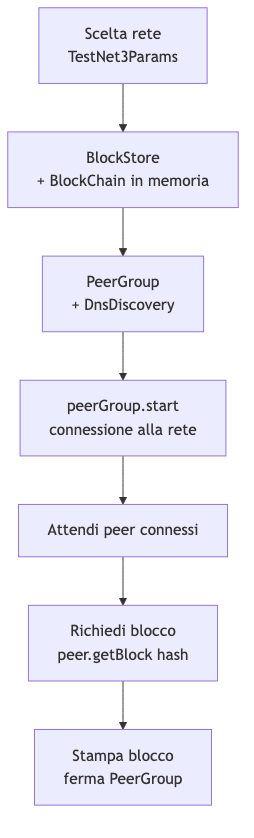
\includegraphics[keepaspectratio,alt={Diagramma Mermaid}]{images/mermaid-lezione-10-lab-bitcoin-con-bitcoinj-01.png}}
\emph{Fig. --- Pipeline dell'esempio di connessione: tutto ruota attorno
a \texttt{PeerGroup}, l'astrazione \texttt{bitcoinj} che gestisce il
pool di connessioni P2P.}

La chiave è il \texttt{PeerGroup}: rappresenta un insieme di connessioni
gestite automaticamente, incluso il mantenimento del numero target di
peer e la ri-connessione in caso di timeout. \texttt{DnsDiscovery} è il
meccanismo di bootstrapping che interroga i seed DNS di cui si è parlato
nella lezione sul layer P2P.

La richiesta del blocco specifico (\texttt{peer.getBlock(hash)})
restituisce un \texttt{Future} --- quindi è asincrona --- e il loop
\texttt{while(flag)} tenta la richiesta su peer diversi finché uno
risponde entro 5 secondi. Questo pattern è tipico delle reti P2P: nessun
peer specifico ha il ``dovere'' di rispondere, quindi il client deve
essere preparato a ritentare.

\begin{calloutwarning}{Blocco di esempio su testnet}

L'hash
\texttt{0000000000000adc6423b570d751efcdf5e019d3d955fee155c28925913cb667}
si riferisce a un blocco \textbf{testnet}, non mainnet. È importante
perché in testnet le regole di PoW sono rilassate (difficulty molto più
bassa) e gli indirizzi hanno un prefisso diverso. Cambiare
\texttt{TestNet3Params} in \texttt{MainNetParams} fa sì che il client si
colleghi alla rete di produzione e tenti di recuperare blocchi reali ---
occhio alla quantità di dati!

\end{calloutwarning}

\begin{center}\rule{0.5\linewidth}{0.5pt}\end{center}

\section{Indirizzi Bitcoin e loro
tipologie}\label{indirizzi-bitcoin-e-loro-tipologie}

Una volta collegati alla rete, la lezione passa a mostrare come generare
chiavi e indirizzi. Prima però viene fatto un rapido ripasso dei tipi di
indirizzo che esistono oggi in Bitcoin mainnet.

\begin{calloutdefinition}{Tipi di indirizzo Bitcoin (mainnet)}

{\def\LTcaptype{none} % do not increment counter
\begin{longtable}[]{@{}
  >{\raggedright\arraybackslash}p{(\linewidth - 4\tabcolsep) * \real{0.3333}}
  >{\raggedright\arraybackslash}p{(\linewidth - 4\tabcolsep) * \real{0.3333}}
  >{\raggedright\arraybackslash}p{(\linewidth - 4\tabcolsep) * \real{0.3333}}@{}}
\toprule\noalign{}
\begin{minipage}[b]{\linewidth}\raggedright
Tipo
\end{minipage} & \begin{minipage}[b]{\linewidth}\raggedright
Prefisso
\end{minipage} & \begin{minipage}[b]{\linewidth}\raggedright
Descrizione
\end{minipage} \\
\midrule\noalign{}
\endhead
\bottomrule\noalign{}
\endlastfoot
\textbf{Legacy P2PKH} & \texttt{1...} & Pay-to-Public-Key-Hash --- il
formato storico \\
\textbf{Legacy P2SH} & \texttt{3...} & Pay-to-Script-Hash --- script
generici (multisig, timelock, \ldots) \\
\textbf{Nested SegWit P2SH-P2WPKH/P2WSH} & \texttt{3...} & SegWit
impacchettato in un P2SH per compatibilità --- solo transizionale \\
\textbf{SegWit nativo P2WPKH/P2WSH} & \texttt{bc1q...} & Bech32, witness
version 0 \\
\textbf{Taproot P2TR} & \texttt{bc1p...} & Bech32m, witness version 1
--- singole firme Schnorr o Tapscript \\
\end{longtable}
}

\end{calloutdefinition}

Il nested SegWit (\texttt{3...}) è stato utile durante la transizione
per permettere a wallet che non conoscevano il nuovo formato
\texttt{bc1q} di inviare fondi a destinatari SegWit, ma oggi è
essenzialmente deprecato: i nuovi wallet preferiscono generare
direttamente \texttt{bc1q} (SegWit v0) o \texttt{bc1p} (Taproot) per
beneficiare delle fee ridotte e delle nuove funzionalità.

\subsection{Generare un indirizzo da una
chiave}\label{generare-un-indirizzo-da-una-chiave}

\begin{Shaded}
\begin{Highlighting}[]
\KeywordTok{public} \DataTypeTok{static} \DataTypeTok{void} \FunctionTok{createNewAddr}\OperatorTok{()} \OperatorTok{\{}
\NormalTok{    NetworkParameters netParams1 }\OperatorTok{=}\NormalTok{ TestNet3Params}\OperatorTok{.}\FunctionTok{get}\OperatorTok{();}

    \BuiltInTok{ECKey}\NormalTok{ key }\OperatorTok{=} \KeywordTok{new} \BuiltInTok{ECKey}\OperatorTok{();}
    \BuiltInTok{System}\OperatorTok{.}\FunctionTok{out}\OperatorTok{.}\FunctionTok{println}\OperatorTok{(}\StringTok{"We created key "} \OperatorTok{+}\NormalTok{ key}\OperatorTok{);}
\NormalTok{    Address addressFromKey }\OperatorTok{=}\NormalTok{ key}\OperatorTok{.}\FunctionTok{toAddress}\OperatorTok{(}\NormalTok{ScriptType}\OperatorTok{.}\FunctionTok{P2PKH}\OperatorTok{,}\NormalTok{ netParams1}\OperatorTok{.}\FunctionTok{network}\OperatorTok{());}

    \BuiltInTok{System}\OperatorTok{.}\FunctionTok{out}\OperatorTok{.}\FunctionTok{println}\OperatorTok{(}\StringTok{"On the "} \OperatorTok{+}\NormalTok{ netParams1}\OperatorTok{.}\FunctionTok{network}\OperatorTok{()} \OperatorTok{+}
        \StringTok{" network, we can use this address "} \OperatorTok{+}\NormalTok{ addressFromKey}\OperatorTok{);}

\NormalTok{    NetworkParameters netParams2 }\OperatorTok{=}\NormalTok{ MainNetParams}\OperatorTok{.}\FunctionTok{get}\OperatorTok{();}
\NormalTok{    addressFromKey }\OperatorTok{=}\NormalTok{ key}\OperatorTok{.}\FunctionTok{toAddress}\OperatorTok{(}\NormalTok{ScriptType}\OperatorTok{.}\FunctionTok{P2PKH}\OperatorTok{,}\NormalTok{ netParams2}\OperatorTok{.}\FunctionTok{network}\OperatorTok{());}
    \BuiltInTok{System}\OperatorTok{.}\FunctionTok{out}\OperatorTok{.}\FunctionTok{println}\OperatorTok{(}\StringTok{"On the "} \OperatorTok{+}\NormalTok{ netParams2}\OperatorTok{.}\FunctionTok{network}\OperatorTok{()} \OperatorTok{+}
        \StringTok{" network, we can use this address "} \OperatorTok{+}\NormalTok{ addressFromKey}\OperatorTok{);}

\NormalTok{    addressFromKey }\OperatorTok{=}\NormalTok{ key}\OperatorTok{.}\FunctionTok{toAddress}\OperatorTok{(}\NormalTok{ScriptType}\OperatorTok{.}\FunctionTok{P2WPKH}\OperatorTok{,}\NormalTok{ netParams2}\OperatorTok{.}\FunctionTok{network}\OperatorTok{());}
    \BuiltInTok{System}\OperatorTok{.}\FunctionTok{out}\OperatorTok{.}\FunctionTok{println}\OperatorTok{(}\StringTok{"On the "} \OperatorTok{+}\NormalTok{ netParams2}\OperatorTok{.}\FunctionTok{network}\OperatorTok{()} \OperatorTok{+}
        \StringTok{" network, we can use this address "} \OperatorTok{+}\NormalTok{ addressFromKey}\OperatorTok{);}
\OperatorTok{\}}
\end{Highlighting}
\end{Shaded}

L'esempio mostra tre cose importanti:

\begin{enumerate}
\def\labelenumi{\arabic{enumi}.}
\tightlist
\item
  \textbf{Una stessa chiave ECDSA}
  (\texttt{ECKey\ key\ =\ new\ ECKey()}) può essere usata per derivare
  più indirizzi.
\item
  Lo stesso hash della chiave pubblica produce \textbf{indirizzi con
  prefisso diverso} a seconda della rete (testnet vs mainnet) perché il
  byte di version cambia.
\item
  Lo stesso hash produce anche \textbf{indirizzi formattati
  diversamente} a seconda dello \texttt{ScriptType} scelto: con
  \texttt{P2PKH} si ottiene un indirizzo legacy \texttt{1...}, con
  \texttt{P2WPKH} si ottiene un SegWit nativo \texttt{bc1q...}. La
  chiave privata è la stessa, ma lo script di lock differisce, e quindi
  cambia l'encoding dell'indirizzo.
\end{enumerate}

\begin{callouttip}{Chiave → indirizzo non è iniettivo sul tipo}

Una stessa chiave genera indirizzi di tipo diverso perché l'indirizzo è
una funzione di (hash della chiave pubblica, tipo di script, rete). Se
si invia denaro al P2PKH di una chiave, non è automaticamente spendibile
con la firma sul P2WPKH della stessa chiave: lo script di unlock è
diverso. Il proprietario della chiave può firmare per entrambi, ma deve
sapere a quale dei suoi indirizzi gli è stato inviato il denaro.

\end{callouttip}

\subsection{Esercizio 1 --- Vanity
address}\label{esercizio-1-vanity-address}

\begin{callouttip}{Esercizio 1: vanity address}

\textbf{Consegna}: scrivere un programma che genera un indirizzo Bitcoin
il cui encoding \textbf{inizia con una stringa scelta} dall'utente (es.
\texttt{1Fabio...}, \texttt{bc1qgold...}).

\textbf{Approccio}: non esiste un modo per costruire una chiave che
produca un indirizzo con un prefisso specifico senza invertire la
funzione hash (cosa infattibile). L'unica strada è \textbf{brute force}:
generare chiavi casuali una dopo l'altra, calcolare l'indirizzo
corrispondente, controllare se inizia con la stringa desiderata, e se no
ripetere.

\begin{Shaded}
\begin{Highlighting}[]
\BuiltInTok{String}\NormalTok{ target }\OperatorTok{=} \StringTok{"1Fab"}\OperatorTok{;}
\ControlFlowTok{while} \OperatorTok{(}\KeywordTok{true}\OperatorTok{)} \OperatorTok{\{}
    \BuiltInTok{ECKey}\NormalTok{ key }\OperatorTok{=} \KeywordTok{new} \BuiltInTok{ECKey}\OperatorTok{();}
\NormalTok{    Address addr }\OperatorTok{=}\NormalTok{ key}\OperatorTok{.}\FunctionTok{toAddress}\OperatorTok{(}\NormalTok{ScriptType}\OperatorTok{.}\FunctionTok{P2PKH}\OperatorTok{,}\NormalTok{ MainNetParams}\OperatorTok{.}\FunctionTok{get}\OperatorTok{().}\FunctionTok{network}\OperatorTok{());}
    \ControlFlowTok{if} \OperatorTok{(}\NormalTok{addr}\OperatorTok{.}\FunctionTok{toString}\OperatorTok{().}\FunctionTok{startsWith}\OperatorTok{(}\NormalTok{target}\OperatorTok{))} \OperatorTok{\{}
        \BuiltInTok{System}\OperatorTok{.}\FunctionTok{out}\OperatorTok{.}\FunctionTok{println}\OperatorTok{(}\StringTok{"Found: "} \OperatorTok{+}\NormalTok{ addr}\OperatorTok{);}
        \BuiltInTok{System}\OperatorTok{.}\FunctionTok{out}\OperatorTok{.}\FunctionTok{println}\OperatorTok{(}\StringTok{"Private key: "} \OperatorTok{+}\NormalTok{ key}\OperatorTok{.}\FunctionTok{getPrivateKeyAsWiF}\OperatorTok{(}\NormalTok{MainNetParams}\OperatorTok{.}\FunctionTok{get}\OperatorTok{().}\FunctionTok{network}\OperatorTok{()));}
        \ControlFlowTok{break}\OperatorTok{;}
    \OperatorTok{\}}
\OperatorTok{\}}
\end{Highlighting}
\end{Shaded}

Il tempo di esecuzione cresce \textbf{esponenzialmente} nella lunghezza
del prefisso (approssimativamente un fattore 58 per ogni carattere
aggiunto nel Base58): 3-4 caratteri si trovano in secondi, 6-7 in
minuti, 10+ richiedono hardware dedicato.

\end{callouttip}

\begin{calloutwarning}{Sicurezza delle vanity address}

Per chiavi cercate brute force su hardware proprio non c'è problema ---
la chiave privata resta locale. Si diffidi però dei servizi online che
generano vanity address ``per conto vostro'': se il servizio genera la
chiave e poi la invia, può trattenerne una copia e svuotare il wallet
quando vi viene inviato denaro. L'unico pattern sicuro è lo
\textbf{split-key vanity}, in cui la parte entropica proviene da voi e
il servizio fornisce solo capacità di calcolo.

\end{calloutwarning}

\begin{center}\rule{0.5\linewidth}{0.5pt}\end{center}

\section{Inspezione del genesis
block}\label{inspezione-del-genesis-block}

L'ultima parte del laboratorio è l'ispezione del blocco 0 di Bitcoin ---
il \textbf{genesis block}, minato da Satoshi Nakamoto il 3 gennaio 2009.

\begin{calloutdefinition}{Genesis block di Bitcoin}

Il blocco con hash
\texttt{0x000000000019d6689c085ae165831e934ff763ae46a2a6c172b3f1b60a8ce26f}
è il primo blocco della blockchain di Bitcoin. È \textbf{hardcoded} nel
codice di ogni client e serve come radice di fiducia da cui far partire
la verifica dell'intera catena. La sua ricompensa coinbase (50 BTC) è
spendibile in teoria ma è considerata non-spendibile di fatto perché
l'UTXO corrispondente non è mai stato incluso nel UTXO set di Bitcoin
Core.

Riferimento:
\href{https://en.bitcoin.it/wiki/Genesis_block}{en.bitcoin.it/wiki/Genesis\_block}

\end{calloutdefinition}

\subsection{Codice per leggere il
genesis}\label{codice-per-leggere-il-genesis}

\begin{Shaded}
\begin{Highlighting}[]
\CommentTok{// 0x000000000019d6689c085ae165831e934ff763ae46a2a6c172b3f1b60a8ce26f}
\KeywordTok{public} \DataTypeTok{static} \DataTypeTok{void} \FunctionTok{getBtcGenesis}\OperatorTok{()} \KeywordTok{throws} \BuiltInTok{InterruptedException} \OperatorTok{\{}
\NormalTok{    NetworkParameters netParams }\OperatorTok{=}\NormalTok{ MainNetParams}\OperatorTok{.}\FunctionTok{get}\OperatorTok{();}

\NormalTok{    Block genesis }\OperatorTok{=}\NormalTok{ netParams}\OperatorTok{.}\FunctionTok{getGenesisBlock}\OperatorTok{();}

    \BuiltInTok{System}\OperatorTok{.}\FunctionTok{out}\OperatorTok{.}\FunctionTok{println}\OperatorTok{(}\NormalTok{genesis}\OperatorTok{);}

\NormalTok{    TransactionInput txIn }\OperatorTok{=}\NormalTok{ genesis}\OperatorTok{.}\FunctionTok{getTransactions}\OperatorTok{().}\FunctionTok{get}\OperatorTok{(}\DecValTok{0}\OperatorTok{).}\FunctionTok{getInput}\OperatorTok{(}\DecValTok{0}\OperatorTok{);}

    \BuiltInTok{System}\OperatorTok{.}\FunctionTok{out}\OperatorTok{.}\FunctionTok{println}\OperatorTok{(}\FunctionTok{bytesToHex}\OperatorTok{(}\NormalTok{txIn}\OperatorTok{.}\FunctionTok{getScriptBytes}\OperatorTok{()));}

    \BuiltInTok{String}\NormalTok{ message }\OperatorTok{=} \FunctionTok{hexToAscii}\OperatorTok{(}\FunctionTok{bytesToHex}\OperatorTok{(}\NormalTok{txIn}\OperatorTok{.}\FunctionTok{getScriptBytes}\OperatorTok{()));}

    \BuiltInTok{System}\OperatorTok{.}\FunctionTok{out}\OperatorTok{.}\FunctionTok{println}\OperatorTok{(}\NormalTok{message}\OperatorTok{);}

    \FunctionTok{printBlockInfo}\OperatorTok{(}\NormalTok{genesis}\OperatorTok{);}
    \FunctionTok{printTxInfo}\OperatorTok{(}\NormalTok{genesis}\OperatorTok{.}\FunctionTok{getTransactions}\OperatorTok{().}\FunctionTok{get}\OperatorTok{(}\DecValTok{0}\OperatorTok{));}
\OperatorTok{\}}

\KeywordTok{public} \DataTypeTok{static} \DataTypeTok{void} \FunctionTok{printBlockInfo}\OperatorTok{(}\NormalTok{Block blk}\OperatorTok{)} \KeywordTok{throws} \BuiltInTok{InterruptedException} \OperatorTok{\{}
    \BuiltInTok{System}\OperatorTok{.}\FunctionTok{out}\OperatorTok{.}\FunctionTok{println}\OperatorTok{(}\StringTok{"Hash       "} \OperatorTok{+}\NormalTok{ blk}\OperatorTok{.}\FunctionTok{getHashAsString}\OperatorTok{());}
    \BuiltInTok{System}\OperatorTok{.}\FunctionTok{out}\OperatorTok{.}\FunctionTok{println}\OperatorTok{(}\StringTok{"Prev Hash  "} \OperatorTok{+}\NormalTok{ blk}\OperatorTok{.}\FunctionTok{getPrevBlockHash}\OperatorTok{());}
    \BuiltInTok{System}\OperatorTok{.}\FunctionTok{out}\OperatorTok{.}\FunctionTok{println}\OperatorTok{(}\StringTok{"Timestamp  "} \OperatorTok{+}\NormalTok{ blk}\OperatorTok{.}\FunctionTok{getTimeSeconds}\OperatorTok{());}
    \BuiltInTok{System}\OperatorTok{.}\FunctionTok{out}\OperatorTok{.}\FunctionTok{println}\OperatorTok{(}\StringTok{"Timestamp  "} \OperatorTok{+}\NormalTok{ blk}\OperatorTok{.}\FunctionTok{time}\OperatorTok{());}
\OperatorTok{\}}
\end{Highlighting}
\end{Shaded}

\subsection{Il messaggio di Satoshi}\label{il-messaggio-di-satoshi}

La parte più suggestiva è la decodifica del \textbf{coinbase script}
della prima (e unica) transazione del genesis block. In una transazione
normale l'input contiene la firma che sblocca l'UTXO speso; in una
coinbase, che non spende nulla, il campo \texttt{scriptSig} è libero e
Satoshi lo ha sfruttato per incidere un messaggio leggibile in ASCII:

\begin{verbatim}
The Times 03/Jan/2009 Chancellor on brink of second bailout for banks
\end{verbatim}

È il titolo del \emph{Times} di Londra di quel giorno. Serve a due
scopi: \textbf{dimostrare che il blocco è stato minato non prima del 3
gennaio 2009} (non si può predire un titolo di giornale futuro), e
lasciare traccia storica del contesto politico-finanziario in cui
Bitcoin nasce --- una risposta esplicita alla crisi bancaria e ai
salvataggi pubblici.

\begin{callouttip}{Timestamping incorporato nel protocollo}

La tecnica di scrivere un riferimento pubblico verificabile (come un
titolo di giornale) in un blocco per dimostrarne la datazione ``non
prima di'' è essenzialmente un \textbf{timestamping crittografico} fatto
in modo manuale. In seguito è stato formalizzato da servizi come
OpenTimestamps, che permettono di inserire hash di documenti arbitrari
nella blockchain di Bitcoin come prova di esistenza a una certa data.

\end{callouttip}

\subsection{Cosa estraiamo dal
genesis}\label{cosa-estraiamo-dal-genesis}

Eseguendo \texttt{printBlockInfo} e \texttt{printTxInfo} si vede
concretamente la struttura di un blocco Bitcoin:

\begin{itemize}
\tightlist
\item
  \textbf{Hash} del blocco ---
  \texttt{000000000019d6689c085ae165831e934ff763ae46a2a6c172b3f1b60a8ce26f}
\item
  \textbf{Prev hash} --- tutti zeri, perché non c'è un blocco precedente
\item
  \textbf{Timestamp} --- 1231006505 secondi Unix, cioè 3 gennaio 2009
  18:15:05 UTC
\item
  \textbf{Transazione coinbase} con il messaggio di cui sopra e un
  output di 50 BTC al public key di Satoshi (in formato P2PK, non P2PKH:
  è lo stile più vecchio)
\end{itemize}

\begin{center}\rule{0.5\linewidth}{0.5pt}\end{center}

\section{Transazioni e SegWit}\label{transazioni-e-segwit}

Nel finale della lezione vengono indicate due risorse per approfondire
ciò che si costruirà nei laboratori successivi (dove si imposteranno
transazioni manualmente):

\begin{itemize}
\tightlist
\item
  \textbf{Deconstructing a Bitcoin transaction} ---
  \href{https://dev.to/thunderbiscuit/deconstructing-a-bitcoin-transaction-4l2n}{dev.to/thunderbiscuit/deconstructing-a-bitcoin-transaction-4l2n}.
  Una spiegazione campo-per-campo di cosa c'è dentro una transazione
  Bitcoin: version, input list (previous outpoint, scriptSig, sequence),
  output list (value, scriptPubKey), locktime. Utile per capire come
  serializzare manualmente una transazione.
\item
  \textbf{SegWit recap} ---
  \href{https://learnmeabitcoin.com/technical/upgrades/segregated-witness/}{learnmeabitcoin.com/technical/upgrades/segregated-witness}.
  Introduzione al segregated witness, l'upgrade del 2017 che ha separato
  i dati di firma (witness) dal resto della transazione, risolvendo la
  transaction malleability e aprendo la strada a Lightning Network.
\end{itemize}

\begin{calloutnote}{Perché serve comprendere SegWit}

Il motivo per cui le slide ripassano SegWit proprio qui è che il tipo di
indirizzo che si genera (\texttt{P2PKH} vs \texttt{P2WPKH}) si riflette
direttamente nella struttura della transazione che lo spende: un P2WPKH
mette la firma nel campo \emph{witness}, non nello \texttt{scriptSig}, e
calcola la fee in base al \emph{virtual size} invece che alla dimensione
grezza. Senza questo contesto, alcuni campi di una transazione moderna
sembrano arbitrari.

\end{calloutnote}

\begin{center}\rule{0.5\linewidth}{0.5pt}\end{center}

\section{Sintesi del laboratorio}\label{sintesi-del-laboratorio}

\begin{calloutnote}{Cosa resta in mano dopo questa lezione}

\begin{itemize}
\tightlist
\item
  Un progetto Java funzionante che si collega alla \textbf{testnet
  Bitcoin} tramite \texttt{bitcoinj} e scarica un blocco richiesto per
  hash
\item
  La capacità di \textbf{generare chiavi ECDSA} e derivarne indirizzi
  legacy (\texttt{P2PKH}) o SegWit nativi (\texttt{P2WPKH}) per mainnet
  o testnet
\item
  Un primo vanity address personale, ottenuto brute-forzando chiavi
  finché il loro indirizzo inizia con un prefisso scelto
\item
  Un'ispezione diretta del \textbf{genesis block} di Bitcoin, con la
  decodifica del messaggio di Satoshi nel coinbase della transazione 0
\item
  Link di riferimento per approfondire la struttura delle transazioni e
  SegWit in vista dei laboratori successivi
\end{itemize}

\end{calloutnote}

\newpage

\chapter{Lezione 11 --- (Lab) Bitcoin Transactions e
Scripts}\label{lezione-11-lab-bitcoin-transactions-e-scripts}

\section{Cosa si è fatto in questa
lezione}\label{cosa-si-uxe8-fatto-in-questa-lezione-1}

Terzo laboratorio Bitcoin: dopo aver fatto conoscenza con
\texttt{bitcoinj} nella lezione precedente (connessione alla rete,
generazione di indirizzi, lettura del genesis block), qui si entra nel
cuore della serializzazione del protocollo. Si scrive codice Java per
\textbf{ispezionare una transazione campo per campo},
\textbf{decodificare gli script} di input e output mostrandoli come
sequenze di opcode leggibili, e si affronta il caso speciale delle
transazioni con \texttt{OP\_RETURN} --- l'opcode usato per inserire dati
arbitrari nella blockchain.

La parte finale è operativa: si scaricano transazioni reali in formato
hex da \texttt{blockchain.info}, si passano al parser di
\texttt{bitcoinj} (\texttt{Transaction.read()}) e si confronta il
risultato con il decoder ufficiale per verificare la correttezza della
propria comprensione del formato binario.

\begin{calloutnote}{Obiettivi concreti del laboratorio}

\begin{itemize}
\tightlist
\item
  Scrivere una funzione \texttt{printTxInfo} che stampa in modo
  leggibile tutti i campi di una \texttt{Transaction} di bitcoinj (hash,
  coinbase flag, weight, witness flag, input/output con script e
  indirizzi)
\item
  Scrivere una funzione \texttt{printScriptAsOpCodes} che trasforma il
  bytecode grezzo di uno script Bitcoin in una sequenza testuale di
  opcode, gestendo correttamente i dati push e l'\texttt{OP\_RETURN}
\item
  Scaricare transazioni reali dalla blockchain in formato \textbf{raw
  hex}, deserializzarle, ispezionarle e verificare il risultato contro
  il decoder pubblico
\item
  Vedere esempi concreti di tre tipi di transazione: \textbf{legacy},
  \textbf{SegWit}, con \textbf{OP\_RETURN}
\end{itemize}

\end{calloutnote}

\begin{center}\rule{0.5\linewidth}{0.5pt}\end{center}

\section{Riferimenti della lezione}\label{riferimenti-della-lezione}

Le slide citano esplicitamente una serie di link che sono il materiale
di studio integrativo al codice mostrato in aula. Vale la pena tenerli a
portata.

Per le \textbf{transazioni} e il loro formato:

\begin{itemize}
\tightlist
\item
  \href{https://dev.to/thunderbiscuit/deconstructing-a-bitcoin-transaction-4l2n}{Deconstructing
  a Bitcoin transaction} --- descrizione campo-per-campo molto chiara
\item
  \href{https://learnmeabitcoin.com/technical/upgrades/segregated-witness/}{SegWit
  recap} --- come il witness cambia la struttura e perché
\end{itemize}

Per gli \textbf{script e gli opcode}:

\begin{itemize}
\tightlist
\item
  \href{https://learnmeabitcoin.com/technical/script/}{Script e opcode
  list} --- ripasso generale
\item
  \href{https://opcodeexplained.com/opcodes/}{Opcode Explained} ---
  lista dettagliata di tutti gli opcode
\item
  \href{https://en.bitcoin.it/wiki/Script}{Bitcoin Wiki --- Script} ---
  riferimento storico canonico
\item
  \href{https://learnmeabitcoin.com/technical/script/return/}{OP\_RETURN}
  --- approfondimento sull'opcode più importante di questa lezione
\end{itemize}

Per l'\textbf{esercitazione pratica}:

\begin{itemize}
\tightlist
\item
  \href{https://blockchain.info/rawtx/a637ad18fabee7ad3ccd51e317091a6e16991311c0c9b83233b140b66b114448?format=hex}{blockchain.info
  raw transaction endpoint} --- esempio che restituisce l'hex della
  transazione
\item
  \href{https://www.blockchain.com/explorer/assets/btc/decode-transaction}{Blockchain.com
  Decode Transaction} --- tool web per verificare la decodifica
\end{itemize}

\begin{center}\rule{0.5\linewidth}{0.5pt}\end{center}

\section{Struttura di una transazione
Bitcoin}\label{struttura-di-una-transazione-bitcoin}

Prima di scrivere codice conviene fissare mentalmente i campi. Una
transazione Bitcoin, nel formato serializzato, si compone di:

\pandocbounded{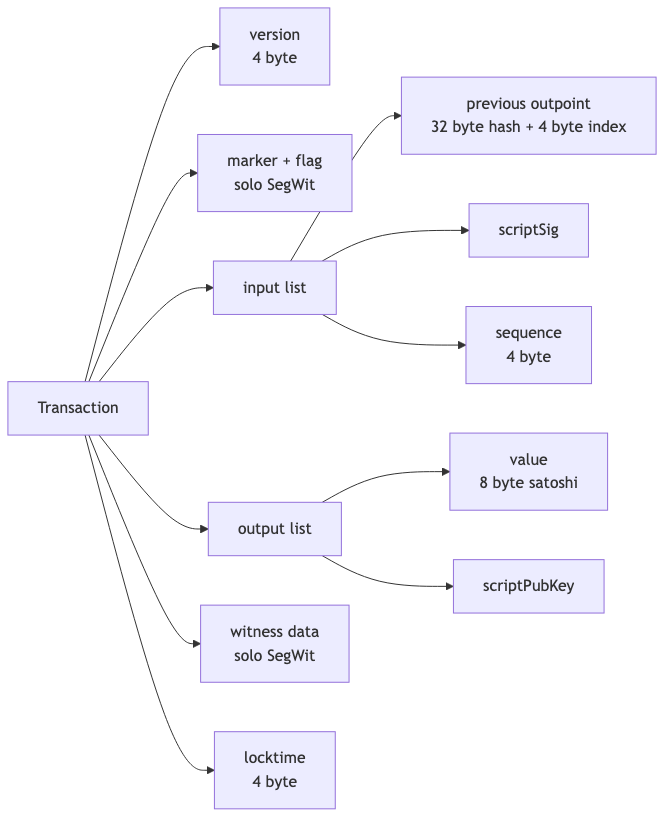
\includegraphics[keepaspectratio,alt={Diagramma Mermaid}]{images/mermaid-lezione-11-lab-bitcoin-transactions-e-scripts-01.png}}
\emph{Fig. --- I campi di una transazione Bitcoin.
\texttt{marker}/\texttt{flag} e \texttt{witness\ data} sono presenti
solo nelle transazioni SegWit.}

La distinzione cruciale per il codice è fra transazione \textbf{legacy}
e \textbf{SegWit}: nelle legacy la firma vive dentro \texttt{scriptSig}
(un campo dell'input); nelle SegWit viene spostata in una sezione
separata (\texttt{witness\ data}) in fondo alla transazione, lasciando
\texttt{scriptSig} vuoto. Questo cambia il layout binario e richiede il
parser di gestire i due casi. Bitcoinj si occupa di distinguerli
automaticamente leggendo il \textbf{marker byte} (\texttt{0x00}) e il
\textbf{flag byte} (\texttt{0x01}) che, se presenti subito dopo la
version, segnalano una transazione SegWit.

\begin{calloutdefinition}{Coinbase transaction}

La prima transazione di ogni blocco è la \textbf{coinbase}, che crea
nuovi bitcoin (il block reward) e non ha un input spendibile precedente:
il suo unico input ha \texttt{previous\ outpoint} con hash tutto-zero e
indice \texttt{0xFFFFFFFF}, e \texttt{scriptSig} è lasciato libero dal
miner per inserirvi dati arbitrari (tipicamente il numero del blocco per
l'altezza --- BIP 34 --- o messaggi testuali, come fece Satoshi nel
genesis).

\end{calloutdefinition}

\begin{center}\rule{0.5\linewidth}{0.5pt}\end{center}

\section{\texorpdfstring{\texttt{printTxInfo} --- stampare una
transazione in modo
leggibile}{printTxInfo --- stampare una transazione in modo leggibile}}\label{printtxinfo-stampare-una-transazione-in-modo-leggibile}

Il primo esercizio di laboratorio è una funzione che prende una
\texttt{Transaction} di bitcoinj e ne stampa tutti i campi in formato
umano. Il valore didattico è che costringe a distinguere i casi
(coinbase vs regolare, con vs senza witness) e a ricavare gli indirizzi
dai rispettivi script.

\begin{Shaded}
\begin{Highlighting}[]
\KeywordTok{public} \DataTypeTok{static} \DataTypeTok{void} \FunctionTok{printTxInfo}\OperatorTok{(}\NormalTok{Transaction tx}\OperatorTok{)} \KeywordTok{throws} \BuiltInTok{InterruptedException} \OperatorTok{\{}
    \CommentTok{// txHash, isCoinbase, weight, hasWitness}
    \BuiltInTok{StringBuilder}\NormalTok{ line }\OperatorTok{=} \KeywordTok{new} \BuiltInTok{StringBuilder}\OperatorTok{();}
    \DataTypeTok{boolean}\NormalTok{ isCoinbase }\OperatorTok{=} \KeywordTok{false}\OperatorTok{;}
    \DataTypeTok{boolean}\NormalTok{ hasWitness }\OperatorTok{=} \KeywordTok{false}\OperatorTok{;}
\NormalTok{    line}\OperatorTok{.}\FunctionTok{append}\OperatorTok{(}\NormalTok{tx}\OperatorTok{.}\FunctionTok{getTxId}\OperatorTok{().}\FunctionTok{toString}\OperatorTok{());}
\NormalTok{    line}\OperatorTok{.}\FunctionTok{append}\OperatorTok{(}\StringTok{","}\OperatorTok{);}
    \ControlFlowTok{if} \OperatorTok{(}\NormalTok{tx}\OperatorTok{.}\FunctionTok{isCoinBase}\OperatorTok{())} \OperatorTok{\{}
\NormalTok{        isCoinbase }\OperatorTok{=} \KeywordTok{true}\OperatorTok{;}
\NormalTok{        line}\OperatorTok{.}\FunctionTok{append}\OperatorTok{(}\StringTok{"1"}\OperatorTok{);}
    \OperatorTok{\}} \ControlFlowTok{else} \OperatorTok{\{}
\NormalTok{        isCoinbase }\OperatorTok{=} \KeywordTok{false}\OperatorTok{;}
\NormalTok{        line}\OperatorTok{.}\FunctionTok{append}\OperatorTok{(}\StringTok{"0"}\OperatorTok{);}
    \OperatorTok{\}}
\NormalTok{    line}\OperatorTok{.}\FunctionTok{append}\OperatorTok{(}\StringTok{","}\OperatorTok{);}
\NormalTok{    line}\OperatorTok{.}\FunctionTok{append}\OperatorTok{(}\StringTok{""} \OperatorTok{+}\NormalTok{ tx}\OperatorTok{.}\FunctionTok{getWeight}\OperatorTok{());}
\NormalTok{    line}\OperatorTok{.}\FunctionTok{append}\OperatorTok{(}\StringTok{","}\OperatorTok{);}
    \ControlFlowTok{if} \OperatorTok{(}\NormalTok{tx}\OperatorTok{.}\FunctionTok{hasWitnesses}\OperatorTok{())} \OperatorTok{\{}
\NormalTok{        hasWitness }\OperatorTok{=} \KeywordTok{true}\OperatorTok{;}
\NormalTok{        line}\OperatorTok{.}\FunctionTok{append}\OperatorTok{(}\StringTok{"1"}\OperatorTok{);}
    \OperatorTok{\}} \ControlFlowTok{else} \OperatorTok{\{}
\NormalTok{        hasWitness }\OperatorTok{=} \KeywordTok{false}\OperatorTok{;}
\NormalTok{        line}\OperatorTok{.}\FunctionTok{append}\OperatorTok{(}\StringTok{"0"}\OperatorTok{);}
    \OperatorTok{\}}
    \BuiltInTok{System}\OperatorTok{.}\FunctionTok{out}\OperatorTok{.}\FunctionTok{println}\OperatorTok{(}\StringTok{"General info : "} \OperatorTok{+}\NormalTok{ line}\OperatorTok{.}\FunctionTok{toString}\OperatorTok{());}

\NormalTok{    line }\OperatorTok{=} \KeywordTok{new} \BuiltInTok{StringBuilder}\OperatorTok{();}
    \ControlFlowTok{if} \OperatorTok{(}\NormalTok{isCoinbase}\OperatorTok{)} \OperatorTok{\{}
        \CommentTok{// check if it has messages inside input scripts}
        \DataTypeTok{boolean}\NormalTok{ first }\OperatorTok{=} \KeywordTok{true}\OperatorTok{;}
        \ControlFlowTok{for} \OperatorTok{(}\NormalTok{TransactionInput ii }\OperatorTok{:}\NormalTok{ tx}\OperatorTok{.}\FunctionTok{getInputs}\OperatorTok{())} \OperatorTok{\{}
            \ControlFlowTok{if} \OperatorTok{(}\NormalTok{first}\OperatorTok{)}\NormalTok{ first }\OperatorTok{=} \KeywordTok{false}\OperatorTok{;}
            \ControlFlowTok{else}\NormalTok{ line}\OperatorTok{.}\FunctionTok{append}\OperatorTok{(}\StringTok{"}\SpecialCharTok{\textbackslash{}n}\StringTok{"}\OperatorTok{);}
\NormalTok{            line}\OperatorTok{.}\FunctionTok{append}\OperatorTok{(}\StringTok{"Coinbase input script message? "} \OperatorTok{+}
                \FunctionTok{hexToAscii}\OperatorTok{(}\FunctionTok{bytesToHex}\OperatorTok{(}\NormalTok{ii}\OperatorTok{.}\FunctionTok{getScriptBytes}\OperatorTok{())));}
        \OperatorTok{\}}
    \OperatorTok{\}} \ControlFlowTok{else} \OperatorTok{\{}
        \CommentTok{// not coinbase so there is at least one input}
        \CommentTok{// prevTx\_Id, prevTxPos, script:}
        \DataTypeTok{boolean}\NormalTok{ first }\OperatorTok{=} \KeywordTok{true}\OperatorTok{;}
        \ControlFlowTok{for} \OperatorTok{(}\NormalTok{TransactionInput ii }\OperatorTok{:}\NormalTok{ tx}\OperatorTok{.}\FunctionTok{getInputs}\OperatorTok{())} \OperatorTok{\{}
            \ControlFlowTok{if} \OperatorTok{(}\NormalTok{first}\OperatorTok{)}\NormalTok{ first }\OperatorTok{=} \KeywordTok{false}\OperatorTok{;}
            \ControlFlowTok{else}\NormalTok{ line}\OperatorTok{.}\FunctionTok{append}\OperatorTok{(}\StringTok{"}\SpecialCharTok{\textbackslash{}n}\StringTok{"}\OperatorTok{);}
\NormalTok{            line}\OperatorTok{.}\FunctionTok{append}\OperatorTok{(}\StringTok{"Prev txHash "} \OperatorTok{+}\NormalTok{ ii}\OperatorTok{.}\FunctionTok{getOutpoint}\OperatorTok{().}\FunctionTok{hash}\OperatorTok{().}\FunctionTok{toString}\OperatorTok{());}
\NormalTok{            line}\OperatorTok{.}\FunctionTok{append}\OperatorTok{(}\StringTok{"}\SpecialCharTok{\textbackslash{}n}\StringTok{Prev txPos  "} \OperatorTok{+}\NormalTok{ ii}\OperatorTok{.}\FunctionTok{getOutpoint}\OperatorTok{().}\FunctionTok{index}\OperatorTok{());}
\NormalTok{            line}\OperatorTok{.}\FunctionTok{append}\OperatorTok{(}\StringTok{"}\SpecialCharTok{\textbackslash{}n}\StringTok{scriptSig   "} \OperatorTok{+} \FunctionTok{bytesToHex}\OperatorTok{(}\NormalTok{ii}\OperatorTok{.}\FunctionTok{getScriptBytes}\OperatorTok{()));}
            \ControlFlowTok{if} \OperatorTok{(}\NormalTok{ii}\OperatorTok{.}\FunctionTok{hasWitness}\OperatorTok{())} \OperatorTok{\{}
\NormalTok{                line}\OperatorTok{.}\FunctionTok{append}\OperatorTok{(}\StringTok{"}\SpecialCharTok{\textbackslash{}n}\StringTok{witness     "} \OperatorTok{+}\NormalTok{ ii}\OperatorTok{.}\FunctionTok{getWitness}\OperatorTok{().}\FunctionTok{toString}\OperatorTok{());}
            \OperatorTok{\}}
        \OperatorTok{\}}
    \OperatorTok{\}}
    \BuiltInTok{System}\OperatorTok{.}\FunctionTok{out}\OperatorTok{.}\FunctionTok{println}\OperatorTok{(}\StringTok{"Inputs :}\SpecialCharTok{\textbackslash{}n}\StringTok{"} \OperatorTok{+}\NormalTok{ line}\OperatorTok{.}\FunctionTok{toString}\OperatorTok{());}

\NormalTok{    line }\OperatorTok{=} \KeywordTok{new} \BuiltInTok{StringBuilder}\OperatorTok{();}
    \CommentTok{// addr, amount, outScriptBytes}
    \CommentTok{// there is always at least one output}
    \DataTypeTok{boolean}\NormalTok{ first }\OperatorTok{=} \KeywordTok{true}\OperatorTok{;}
    \ControlFlowTok{for} \OperatorTok{(}\NormalTok{TransactionOutput oo }\OperatorTok{:}\NormalTok{ tx}\OperatorTok{.}\FunctionTok{getOutputs}\OperatorTok{())} \OperatorTok{\{}
        \ControlFlowTok{if} \OperatorTok{(}\NormalTok{first}\OperatorTok{)}\NormalTok{ first }\OperatorTok{=} \KeywordTok{false}\OperatorTok{;}
        \ControlFlowTok{else}\NormalTok{ line}\OperatorTok{.}\FunctionTok{append}\OperatorTok{(}\StringTok{"}\SpecialCharTok{\textbackslash{}n}\StringTok{"}\OperatorTok{);}
        \DataTypeTok{byte}\OperatorTok{[]}\NormalTok{ outScript }\OperatorTok{=}\NormalTok{ oo}\OperatorTok{.}\FunctionTok{getScriptBytes}\OperatorTok{();}
        \BuiltInTok{String}\NormalTok{ outAddr }\OperatorTok{=}\NormalTok{ ScriptParser}\OperatorTok{.}\FunctionTok{addrFromOut}\OperatorTok{(}\NormalTok{outScript}\OperatorTok{);}
        \DataTypeTok{int}\NormalTok{ outType }\OperatorTok{=}\NormalTok{ ScriptParser}\OperatorTok{.}\FunctionTok{typeFromOut}\OperatorTok{(}\NormalTok{outScript}\OperatorTok{);}
        \ControlFlowTok{if} \OperatorTok{(}\NormalTok{outAddr }\OperatorTok{==} \KeywordTok{null}\OperatorTok{)} \OperatorTok{\{}
            \CommentTok{// writes \textquotesingle{}\#UNKNOWN\#\textquotesingle{} as address if not decodable}
\NormalTok{            outAddr }\OperatorTok{=} \StringTok{"\#UNKNOWN\#"}\OperatorTok{;}
        \OperatorTok{\}}
\NormalTok{        line}\OperatorTok{.}\FunctionTok{append}\OperatorTok{(}\StringTok{"Addr "} \OperatorTok{+}\NormalTok{ outAddr}\OperatorTok{);}
\NormalTok{        line}\OperatorTok{.}\FunctionTok{append}\OperatorTok{(}\StringTok{"}\SpecialCharTok{\textbackslash{}n}\StringTok{Amount "} \OperatorTok{+}\NormalTok{ oo}\OperatorTok{.}\FunctionTok{getValue}\OperatorTok{().}\FunctionTok{getValue}\OperatorTok{());}
\NormalTok{        line}\OperatorTok{.}\FunctionTok{append}\OperatorTok{(}\StringTok{"}\SpecialCharTok{\textbackslash{}n}\StringTok{script "} \OperatorTok{+} \FunctionTok{bytesToHex}\OperatorTok{(}\NormalTok{outScript}\OperatorTok{));}
\NormalTok{        line}\OperatorTok{.}\FunctionTok{append}\OperatorTok{(}\StringTok{"}\SpecialCharTok{\textbackslash{}n}\StringTok{script "} \OperatorTok{+} \FunctionTok{printScriptAsOpCodes}\OperatorTok{(}\NormalTok{outScript}\OperatorTok{));}
\NormalTok{        line}\OperatorTok{.}\FunctionTok{append}\OperatorTok{(}\StringTok{"}\SpecialCharTok{\textbackslash{}n}\StringTok{script type "} \OperatorTok{+}\NormalTok{ ScriptTypeCustom}\OperatorTok{.}\FunctionTok{typeName}\OperatorTok{(}\NormalTok{outType}\OperatorTok{));}
    \OperatorTok{\}}
    \BuiltInTok{System}\OperatorTok{.}\FunctionTok{out}\OperatorTok{.}\FunctionTok{println}\OperatorTok{(}\StringTok{"Outputs :}\SpecialCharTok{\textbackslash{}n}\StringTok{"} \OperatorTok{+}\NormalTok{ line}\OperatorTok{.}\FunctionTok{toString}\OperatorTok{());}
\OperatorTok{\}}
\end{Highlighting}
\end{Shaded}

\subsection{Cosa vale la pena notare}\label{cosa-vale-la-pena-notare}

\begin{itemize}
\tightlist
\item
  \textbf{\texttt{getTxId()}} restituisce il doppio SHA-256 dei campi
  ``non witness'' della transazione. Per le SegWit è utile perché rende
  l'ID immune dalla \emph{malleability}: modificare la firma non cambia
  l'ID della transazione.
\item
  \textbf{\texttt{getWeight()}} è la metrica usata da Bitcoin per
  calcolare le fee dopo SegWit: i byte witness contano 1, quelli
  non-witness contano 4. Il limite di blocco è 4M weight units.
\item
  \textbf{Caso coinbase}: si stampa il contenuto dello
  \texttt{scriptSig} interpretato come ASCII, per vedere l'eventuale
  messaggio del miner. È lo stesso trucco con cui si è letto il
  \texttt{Chancellor\ on\ brink\ of\ second\ bailout\ for\ banks} nel
  genesis.
\item
  \textbf{Caso regolare}: per ogni input si stampa la coppia
  \texttt{(prev\ hash,\ prev\ index)} che identifica l'UTXO speso, il
  \texttt{scriptSig} in hex, e il witness se presente.
\item
  \textbf{Per gli output}: si usa un \texttt{ScriptParser} custom che
  tenta di decodificare lo \texttt{scriptPubKey} in un indirizzo. Se lo
  script non corrisponde a un pattern noto (non è P2PKH, P2SH, P2WPKH,
  \ldots) si scrive \texttt{\#UNKNOWN\#} invece di inventare un
  indirizzo.
\end{itemize}

\begin{callouttip}{Indirizzo = pattern riconosciuto nello script}

Un \textbf{indirizzo non è un campo della transazione}: è una
\textbf{reinterpretazione} dello \texttt{scriptPubKey} quando
quest'ultimo ha una forma ``nota''.
\texttt{OP\_DUP\ OP\_HASH160\ \textless{}20B\textgreater{}\ OP\_EQUALVERIFY\ OP\_CHECKSIG}
→ P2PKH, \texttt{OP\_HASH160\ \textless{}20B\textgreater{}\ OP\_EQUAL} →
P2SH, e così via. Se lo script è arbitrario (es. un multisig bare, un
timelock), non c'è un indirizzo standard da mostrare.

\end{callouttip}

\begin{center}\rule{0.5\linewidth}{0.5pt}\end{center}

\section{\texorpdfstring{\texttt{printScriptAsOpCodes} --- decodificare
uno script
Bitcoin}{printScriptAsOpCodes --- decodificare uno script Bitcoin}}\label{printscriptasopcodes-decodificare-uno-script-bitcoin}

Gli script di Bitcoin sono sequenze di byte che il parser deve
interpretare come un misto di \textbf{opcode} (singoli byte con nome
simbolico) e \textbf{push di dati} (un byte che dichiara la lunghezza,
seguito dai dati). La funzione mostrata in aula fa proprio questo.

\begin{Shaded}
\begin{Highlighting}[]
\KeywordTok{public} \DataTypeTok{static} \BuiltInTok{String} \FunctionTok{printScriptAsOpCodes}\OperatorTok{(}\DataTypeTok{byte}\OperatorTok{[]}\NormalTok{ script}\OperatorTok{)} \OperatorTok{\{}
    \BuiltInTok{StringBuilder}\NormalTok{ line }\OperatorTok{=} \KeywordTok{new} \BuiltInTok{StringBuilder}\OperatorTok{();}
    \ControlFlowTok{for} \OperatorTok{(}\DataTypeTok{int}\NormalTok{ i }\OperatorTok{=} \DecValTok{0}\OperatorTok{;}\NormalTok{ i }\OperatorTok{\textless{}}\NormalTok{ script}\OperatorTok{.}\FunctionTok{length}\OperatorTok{;)} \OperatorTok{\{}
        \DataTypeTok{int}\NormalTok{ val }\OperatorTok{=} \BuiltInTok{Utilities}\OperatorTok{.}\FunctionTok{readUnsignedByte}\OperatorTok{(}\NormalTok{script}\OperatorTok{[}\NormalTok{i}\OperatorTok{]);}
\NormalTok{        line}\OperatorTok{.}\FunctionTok{append}\OperatorTok{(}\NormalTok{ScriptOpCodes}\OperatorTok{.}\FunctionTok{getOpCodeName}\OperatorTok{(}\NormalTok{val}\OperatorTok{));}
\NormalTok{        line}\OperatorTok{.}\FunctionTok{append}\OperatorTok{(}\StringTok{" "}\OperatorTok{);}
\NormalTok{        i}\OperatorTok{++;}
        \ControlFlowTok{if} \OperatorTok{((}\NormalTok{val }\OperatorTok{\textgreater{}=} \DecValTok{1}\OperatorTok{)} \OperatorTok{\&\&} \OperatorTok{(}\NormalTok{val }\OperatorTok{\textless{}=} \DecValTok{75}\OperatorTok{))} \OperatorTok{\{}
            \ControlFlowTok{for} \OperatorTok{(}\DataTypeTok{int}\NormalTok{ j }\OperatorTok{=} \DecValTok{0}\OperatorTok{;}\NormalTok{ j }\OperatorTok{\textless{}}\NormalTok{ val}\OperatorTok{;}\NormalTok{ j}\OperatorTok{++)} \OperatorTok{\{}
\NormalTok{                line}\OperatorTok{.}\FunctionTok{append}\OperatorTok{(}\FunctionTok{byteToHex}\OperatorTok{(}\NormalTok{script}\OperatorTok{[}\NormalTok{i}\OperatorTok{]));}
\NormalTok{                line}\OperatorTok{.}\FunctionTok{append}\OperatorTok{(}\StringTok{" "}\OperatorTok{);}
\NormalTok{                i}\OperatorTok{++;}
            \OperatorTok{\}}
        \OperatorTok{\}} \ControlFlowTok{else} \ControlFlowTok{if} \OperatorTok{(}\NormalTok{val }\OperatorTok{==} \DecValTok{106}\OperatorTok{)} \OperatorTok{\{}
            \ControlFlowTok{while} \OperatorTok{(}\NormalTok{i }\OperatorTok{\textless{}}\NormalTok{ script}\OperatorTok{.}\FunctionTok{length}\OperatorTok{)} \OperatorTok{\{}
\NormalTok{                line}\OperatorTok{.}\FunctionTok{append}\OperatorTok{(}\FunctionTok{hexToAscii}\OperatorTok{(}\FunctionTok{byteToHex}\OperatorTok{(}\NormalTok{script}\OperatorTok{[}\NormalTok{i}\OperatorTok{])));}
\NormalTok{                line}\OperatorTok{.}\FunctionTok{append}\OperatorTok{(}\StringTok{" "}\OperatorTok{);}
\NormalTok{                i}\OperatorTok{++;}
            \OperatorTok{\}}
        \OperatorTok{\}}
    \OperatorTok{\}}
    \ControlFlowTok{return}\NormalTok{ line}\OperatorTok{.}\FunctionTok{toString}\OperatorTok{();}
\OperatorTok{\}}
\end{Highlighting}
\end{Shaded}

\subsection{Logica del parser}\label{logica-del-parser}

Il parser ha tre rami:

\begin{itemize}
\tightlist
\item
  \textbf{Byte 1--75}: è un'istruzione implicita
  \texttt{OP\_PUSHBYTES\_N} --- il byte stesso indica quanti byte
  successivi sono dati da pushare nello stack. Si stampano come hex.
\item
  \textbf{Byte 106 (\texttt{OP\_RETURN})}: segnala che la transazione è
  ``unspendable'' e che tutto ciò che segue sullo script è \textbf{puro
  dato arbitrario}, interpretato come ASCII (per comodità: qualsiasi
  contenuto è ammesso).
\item
  \textbf{Altri opcode}: si stampa solo il nome simbolico (es.
  \texttt{OP\_DUP}, \texttt{OP\_HASH160}, \texttt{OP\_CHECKSIG}).
\end{itemize}

\begin{calloutwarning}{Parser semplificato}

La funzione non gestisce gli opcode di push a lunghezza esplicita
(\texttt{OP\_PUSHDATA1}, \texttt{OP\_PUSHDATA2}, \texttt{OP\_PUSHDATA4},
valori 76-78), che servono a pushare quantità di dati superiori a 75
byte. Per uno script P2PKH o P2SH standard non è un problema --- gli
hash sono 20 byte e le firme stanno sotto i 75. Per script più
complessi, come alcuni \texttt{OP\_RETURN} con payload grande,
bisognerebbe estendere il parser.

\end{calloutwarning}

\subsection{\texorpdfstring{Esempio: decodifica di uno
\texttt{scriptPubKey}
P2PKH}{Esempio: decodifica di uno scriptPubKey P2PKH}}\label{esempio-decodifica-di-uno-scriptpubkey-p2pkh}

Prendendo un output di tipo P2PKH, lo \texttt{scriptPubKey} in hex è
tipicamente:

\begin{verbatim}
76 a9 14 <20-byte-hash> 88 ac
\end{verbatim}

Passato a \texttt{printScriptAsOpCodes} restituisce:

\begin{verbatim}
OP_DUP OP_HASH160 OP_PUSHBYTES_20 <hex dell'hash> OP_EQUALVERIFY OP_CHECKSIG
\end{verbatim}

--- che è esattamente lo script canonico di pagamento a hash di chiave
pubblica.

\begin{center}\rule{0.5\linewidth}{0.5pt}\end{center}

\section{OP\_RETURN: dati arbitrari sulla
blockchain}\label{op_return-dati-arbitrari-sulla-blockchain}

\begin{calloutdefinition}{OP\_RETURN}

\texttt{OP\_RETURN} (opcode \texttt{0x6A}, decimale 106) termina
immediatamente l'esecuzione dello script facendolo \textbf{fallire
sempre}. Un output il cui \texttt{scriptPubKey} inizia con
\texttt{OP\_RETURN} non è mai spendibile: non esiste alcuna sequenza di
\texttt{scriptSig} che possa farlo valutare a \texttt{true}. In
compenso, i nodi Bitcoin accettano in coda all'opcode \textbf{fino a 80
byte} di dati arbitrari, che vengono così incisi permanentemente nella
blockchain.

\end{calloutdefinition}

Il caso d'uso tipico è \textbf{timestamping}: si prende l'hash di un
documento, lo si inserisce come payload di un \texttt{OP\_RETURN}, si
firma la transazione. Da quel momento esiste una prova pubblica e
immutabile che il documento esisteva al timestamp del blocco che
contiene la transazione. È l'idea alla base di servizi come
\href{https://opentimestamps.org/}{OpenTimestamps}.

\begin{callouttip}{Perché OP\_RETURN invece di mettere i dati nello scriptSig}

Si potrebbe teoricamente mettere dati arbitrari nello \texttt{scriptSig}
di un input, ma quell'approccio crea \textbf{UTXO non spendibili che
restano nel UTXO set} per sempre, gonfiandolo inutilmente.
\texttt{OP\_RETURN} è riconosciuto dai nodi come \emph{provably
unspendable}: l'output associato viene \textbf{escluso dal UTXO set},
quindi non pesa sulle prestazioni della rete. È la ragione per cui
Bitcoin Core lo ha standardizzato.

\end{callouttip}

\begin{center}\rule{0.5\linewidth}{0.5pt}\end{center}

\section{Parte operativa: leggere transazioni
reali}\label{parte-operativa-leggere-transazioni-reali}

L'ultima parte del laboratorio consiste nello scaricare transazioni vere
dalla blockchain di produzione e farle digerire al parser. Il metodo è:

\begin{enumerate}
\def\labelenumi{\arabic{enumi}.}
\tightlist
\item
  Prendere un TXID noto (anche da un explorer)
\item
  Chiedere l'hex grezzo con
  \texttt{https://blockchain.info/rawtx/\textless{}txid\textgreater{}?format=hex}
\item
  Passarlo a \texttt{bitcoinj} con \texttt{Transaction.read()}
\item
  Stampare con \texttt{printTxInfo}
\item
  Verificare il risultato con il
  \href{https://www.blockchain.com/explorer/assets/btc/decode-transaction}{decoder
  ufficiale} di blockchain.com
\end{enumerate}

\subsection{Il codice mostrato}\label{il-codice-mostrato}

\begin{Shaded}
\begin{Highlighting}[]
\KeywordTok{public} \DataTypeTok{static} \DataTypeTok{void} \FunctionTok{readRawTx}\OperatorTok{()} \KeywordTok{throws} \BuiltInTok{InterruptedException} \OperatorTok{\{}

    \CommentTok{// String rawHex = "020000000180b98c54dbab5106d5a1449f4e5fdb9146deca1d48e93d66}
    \CommentTok{// 6c5d9290b7c37a3f010000006b483045022100f0e32ceb205a5056694611afcffe4c1f0e63e9c5738}
    \CommentTok{// 2607045ff2c3d9b5b7b3f0220111f0323e56d7462a9299833166569f1a68e1f5090b49bea64f541c4}
    \CommentTok{// 94109c6c012102d0648f06a31d47112f1ff7848c85ce54b772c513bc3337c98f081c19d3dca260fff}
    \CommentTok{// fffff02006d7c4d000000001976a91474d463a046e3175142464740db692fa0762a93e88accad5e5}
    \CommentTok{// f1b50000001976a914c98fc6bd9c2fd88533f28e6797cfa2a0a0e18ecf88ac00000000";}

    \CommentTok{// first segwit}
    \CommentTok{// dfcec48bb8491856c353306ab5febeb7e99e4d783eedf3de98f3ee0812b92bad}
    \CommentTok{// String rawHex = "01000000000101740e5e391018c5e9dc79f324f9607c9c46d21b02f66da}
    \CommentTok{// baa870b4add871d6379f01000000171600148d7a0a3461e3891723e5fdf8129caa0075060cffffff}
    \CommentTok{// fff01fcf60200000000001600148d7a0a3461e3891723e5fdf8129caa0075060cff02483045022100}
    \CommentTok{// 88025cffdaf69d310c6fed11832edd9c19b6a912c132262701ad0e6133227d9202207d73bbf777abd}
    \CommentTok{// 2aeae995d684e6bb1a048c5ac722e16de48bdd35643df7decf001210283409659355b6d1cc3c32dec}
    \CommentTok{// d5d561abaac86c37a353b52895a5e6c196d6f44800000000";}

    \CommentTok{// opreturn}
    \CommentTok{// d84f8cf06829c7202038731e5444411adc63a6d4cbf8d4361b86698abad3a68a}
    \BuiltInTok{String}\NormalTok{ rawHex }\OperatorTok{=} \StringTok{"010000000178ded99d5bd03110a4e43d2cd7cddb3032af3e362d12ed0b8d"}
        \OperatorTok{+} \StringTok{"35cf811baf00255600000004948304502210fc323c40c6eb030c405bbacb478e6848b115c2bdbc5f7"}
        \OperatorTok{+} \StringTok{"8b275072ccecccacaf8a02207102afeb0a16c2caf7dd07a06d642d1ee0286ebe5f7c4d7092c78af4b0"}
        \OperatorTok{+} \StringTok{"4a44e101ffffffff02e80300000000000001976a9140910f9bbafabf5f653080ba23487d80a1dca614"}
        \OperatorTok{+} \StringTok{"388ac00000000000000000a6a084557204369616Ff2100000000"}\OperatorTok{;}

    \DataTypeTok{byte}\OperatorTok{[]}\NormalTok{ ba }\OperatorTok{=} \FunctionTok{hexStringToByteArray}\OperatorTok{(}\NormalTok{rawHex}\OperatorTok{);}
    \BuiltInTok{ByteBuffer}\NormalTok{ bf }\OperatorTok{=} \BuiltInTok{ByteBuffer}\OperatorTok{.}\FunctionTok{wrap}\OperatorTok{(}\NormalTok{ba}\OperatorTok{);}
\NormalTok{    Transaction tx }\OperatorTok{=}\NormalTok{ Transaction}\OperatorTok{.}\FunctionTok{read}\OperatorTok{(}\NormalTok{bf}\OperatorTok{);}
    \BuiltInTok{System}\OperatorTok{.}\FunctionTok{out}\OperatorTok{.}\FunctionTok{println}\OperatorTok{(}\StringTok{"Tx ID: "} \OperatorTok{+}\NormalTok{ tx}\OperatorTok{.}\FunctionTok{getTxId}\OperatorTok{());}
    \BuiltInTok{System}\OperatorTok{.}\FunctionTok{out}\OperatorTok{.}\FunctionTok{println}\OperatorTok{(}\StringTok{"Inputs: "} \OperatorTok{+}\NormalTok{ tx}\OperatorTok{.}\FunctionTok{getInputs}\OperatorTok{().}\FunctionTok{size}\OperatorTok{());}
    \BuiltInTok{System}\OperatorTok{.}\FunctionTok{out}\OperatorTok{.}\FunctionTok{println}\OperatorTok{(}\StringTok{"Inputs: "} \OperatorTok{+}\NormalTok{ tx}\OperatorTok{.}\FunctionTok{getOutputs}\OperatorTok{().}\FunctionTok{size}\OperatorTok{());}
    \FunctionTok{printTxInfo}\OperatorTok{(}\NormalTok{tx}\OperatorTok{);}
\OperatorTok{\}}
\end{Highlighting}
\end{Shaded}

\subsection{Le tre transazioni di
esempio}\label{le-tre-transazioni-di-esempio}

Il docente presenta tre rawHex commentati, uno per ogni caso
significativo:

{\def\LTcaptype{none} % do not increment counter
\begin{longtable}[]{@{}
  >{\raggedright\arraybackslash}p{(\linewidth - 4\tabcolsep) * \real{0.3333}}
  >{\raggedright\arraybackslash}p{(\linewidth - 4\tabcolsep) * \real{0.3333}}
  >{\raggedright\arraybackslash}p{(\linewidth - 4\tabcolsep) * \real{0.3333}}@{}}
\toprule\noalign{}
\begin{minipage}[b]{\linewidth}\raggedright
Caso
\end{minipage} & \begin{minipage}[b]{\linewidth}\raggedright
TXID
\end{minipage} & \begin{minipage}[b]{\linewidth}\raggedright
Cosa mostra
\end{minipage} \\
\midrule\noalign{}
\endhead
\bottomrule\noalign{}
\endlastfoot
\textbf{Legacy} (quello attivo nell'esempio iniziale) & --- & Struttura
classica: input con \texttt{scriptSig} pieno, nessun witness, un paio di
output P2PKH \\
\textbf{SegWit} (primo esempio SegWit del docente) &
\texttt{dfcec48b…bad} & Marker \texttt{0x00} + flag \texttt{0x01} dopo
la version, \texttt{scriptSig} vuoto, firma spostata nel witness alla
fine \\
\textbf{OP\_RETURN} & \texttt{d84f8cf0…68a} & Uno degli output è un
\texttt{OP\_RETURN} con payload ASCII decodificabile \\
\end{longtable}
}

\begin{callouttip}{Workflow di verifica}

\begin{enumerate}
\def\labelenumi{\arabic{enumi}.}
\tightlist
\item
  Scommentare uno dei tre rawHex nel codice
\item
  Eseguire \texttt{readRawTx()} e leggere l'output stampato
\item
  Aprire nel browser
  \texttt{blockchain.com/explorer/assets/btc/decode-transaction}
\item
  Incollare lo stesso rawHex e confrontare i campi: version, input
  count, output count, TXID, tipo di script per ogni output
\item
  Se il codice è corretto, i due output coincidono campo per campo
\end{enumerate}

\end{callouttip}

\begin{center}\rule{0.5\linewidth}{0.5pt}\end{center}

\section{Sintesi operativa}\label{sintesi-operativa}

\begin{calloutnote}{Cosa resta in mano dopo il laboratorio}

\begin{itemize}
\tightlist
\item
  Un parser Java che prende una \texttt{Transaction} di bitcoinj e ne
  stampa tutti i campi (TXID, weight, coinbase flag, witness flag, input
  con previous outpoint e scriptSig/witness, output con indirizzo
  decodificato e script in opcode)
\item
  Un decodificatore di script Bitcoin che gestisce push di dati (1--75
  byte) e il caso speciale di \texttt{OP\_RETURN} (106)
\item
  La capacità di scaricare una transazione arbitraria dalla blockchain
  tramite l'endpoint raw di \texttt{blockchain.info}, deserializzarla
  con \texttt{Transaction.read()} e confrontare il risultato con il
  decoder ufficiale
\item
  Tre esempi concreti --- legacy, SegWit, OP\_RETURN --- che coprono i
  casi significativi che capiterà di incontrare nelle lezioni successive
  sugli Advanced Bitcoin Scripts
\end{itemize}

\end{calloutnote}

\newpage

\chapter{Bitcoin Mining}\label{bitcoin-mining}

\section{Consenso Tradizionale vs Consenso di
Nakamoto}\label{consenso-tradizionale-vs-consenso-di-nakamoto}

Gli algoritmi di consenso classici --- Paxos, Raft, PBFT --- sono
progettati per ambienti \textbf{chiusi}: i nodi sono noti in anticipo,
ciascuno conosce l'identità degli altri e i canali di comunicazione sono
autenticati. Funzionano bene per database distribuiti, state machine
replication, sincronizzazione di orologi.

Le blockchain permissionless come Bitcoin operano in un contesto
radicalmente diverso: nodi anonimi, churn elevato, nessun canale
autenticato, nessuna sincronizzazione degli orologi, nessuna lista di
partecipanti. I protocolli tradizionali semplicemente non si applicano.

\begin{calloutdefinition}{Consenso di Nakamoto}

Un approccio ``implicito'' al consenso: nessuna votazione, nessuno
scambio di messaggi collettivo. Garantisce \emph{eventual consistency}
--- i nodi possono avere visioni temporaneamente divergenti del
registro, ma alla fine convergeranno tutti sulla stessa cronologia, a
patto che la maggioranza della potenza computazionale sia onesta.

\end{calloutdefinition}

Come osservato in lezione: la decentralizzazione di Bitcoin non è
raggiunta con metodi puramente tecnici, ma con una combinazione di
crittografia e \emph{clever incentive engineering}.

\begin{center}\rule{0.5\linewidth}{0.5pt}\end{center}

\section{Il Problema del Double
Spending}\label{il-problema-del-double-spending}

Senza consenso, il sistema crollerebbe immediatamente. Immaginiamo che
Bob invii bitcoin ad Alice (transazione ``verde''), propagata nel
network. Subito dopo Bob prova a spendere gli stessi bitcoin con July
(transazione ``rossa''), propagata da un altro nodo. Nodi diversi
riceverebbero le due transazioni in ordine diverso e i loro registri
divergerebbero --- impossibile capire quale sia quella valida.

La \textbf{MemPool} (\emph{Memory Pool}) è la ``sala d'attesa'' in RAM
di ogni nodo: contiene le transazioni ricevute ma non ancora incluse in
un blocco. È importante sottolineare che la MemPool \textbf{non è l'UTXO
set}: quest'ultimo contiene le transazioni già confermate nella
blockchain, mentre la MemPool è un buffer temporaneo di transazioni in
attesa di conferma. Funziona come una \emph{clearing house}: quando un
nodo riceve una transazione in conflitto con una già presente nella sua
MemPool, la scarta immediatamente. Ma questo risolve solo il problema
locale --- il consenso globale richiede qualcosa di più.

\begin{center}\rule{0.5\linewidth}{0.5pt}\end{center}

\section{Mining: la Lotteria della
Blockchain}\label{mining-la-lotteria-della-blockchain}

I nodi competono per estrarre transazioni dalla propria MemPool e
aggiungerle al registro. Questa competizione è il \textbf{mining}: una
lotteria in cui il vincitore ha il diritto di proporre il blocco
successivo e lo trasmette in broadcast alla rete.

Quando un nodo riceve un nuovo blocco valido, elimina dalla propria
MemPool tutte le transazioni ora confermate e quelle in conflitto ---
garantendo che il double spending tentato da Bob venga neutralizzato.

\begin{center}\rule{0.5\linewidth}{0.5pt}\end{center}

\section{Anatomia di un Blocco}\label{anatomia-di-un-blocco}

Il miner riempie un \textbf{blocco candidato} con transazioni dalla
MemPool, poi costruisce il \textbf{Block Header}: un riassunto compatto
dei metadati (circa 1000 volte più piccolo della lista delle
transazioni).

{\def\LTcaptype{none} % do not increment counter
\begin{longtable}[]{@{}
  >{\raggedright\arraybackslash}p{(\linewidth - 4\tabcolsep) * \real{0.3333}}
  >{\raggedright\arraybackslash}p{(\linewidth - 4\tabcolsep) * \real{0.3333}}
  >{\raggedright\arraybackslash}p{(\linewidth - 4\tabcolsep) * \real{0.3333}}@{}}
\toprule\noalign{}
\begin{minipage}[b]{\linewidth}\raggedright
Campo
\end{minipage} & \begin{minipage}[b]{\linewidth}\raggedright
Dimensione
\end{minipage} & \begin{minipage}[b]{\linewidth}\raggedright
Descrizione
\end{minipage} \\
\midrule\noalign{}
\endhead
\bottomrule\noalign{}
\endlastfoot
\textbf{Magic Number} & 4 byte & Identificatore costante della rete
Bitcoin \\
\textbf{Block Size} & 4 byte & Dimensione totale del blocco \\
\textbf{Version} & 4 byte & Versione del protocollo; gestisce soft/hard
fork \\
\textbf{Previous Block Hash} & 32 byte & Hash SHA-256 dell'header del
blocco precedente --- il ``link'' crittografico della catena \\
\textbf{Merkle Root} & 32 byte & Radice del Merkle Tree delle
transazioni; qualsiasi modifica a una transazione altera questo
valore \\
\textbf{Timestamp} & 4 byte & Secondi Unix dalla mezzanotte del 1 gen
1970; usato per calibrare la difficoltà \\
\textbf{Difficulty Target} & 4 byte & Soglia al di sotto della quale
deve cadere l'hash del blocco \\
\textbf{Nonce} & 4 byte & Il valore che il miner modifica iterativamente
per trovare la soluzione \\
\textbf{Transaction Counter} & 1--9 byte & Numero di transazioni nel
blocco \\
\textbf{Transactions List} & Variabile (fino a 1 MB) & L'elenco
effettivo delle transazioni \\
\end{longtable}
}

Perché raggruppare in blocchi e non minare singole transazioni? Una
catena di hash su blocchi è molto più corta di una su milioni di
transazioni, rendendo la verifica esponenzialmente più rapida. Blocchi
più grandi significano anche trasmissioni di rete più efficienti.

\begin{center}\rule{0.5\linewidth}{0.5pt}\end{center}

\section{Proof of Work: Meccanica e
Complessità}\label{proof-of-work-meccanica-e-complessituxe0}

\begin{calloutdefinition}{Proof of Work}

Funzione \(F_d(c, x) \to \{\text{true, false}\}\) dove \(d\) è la
difficoltà, \(c\) è la challenge (l'header del blocco senza il nonce) e
\(x\) è il \textbf{nonce} da trovare. Calcolare \(F_d\) con \(x\) noto è
rapido; trovare \(x\) tale che il risultato sia ``true'' è
computazionalmente difficile.

\end{calloutdefinition}

Il procedimento del miner:

\begin{enumerate}
\def\labelenumi{\arabic{enumi}.}
\tightlist
\item
  Imposta il nonce a 0
\item
  Calcola \texttt{SHA256(SHA256(Block-Header\ +\ Nonce))}
\item
  Se l'hash è \textbf{inferiore al Target} → blocco valido, trasmetti
\item
  Altrimenti, incrementa il nonce di 1 e ripeti
\end{enumerate}

Ogni singolo bit dell'hash a 256 bit è indipendente dagli altri --- come
il lancio di una moneta. Non esistono scorciatoie: l'unico metodo è la
forza bruta. La probabilità che un hash casuale cada sotto la soglia
\(T\) è:

\[p = \frac{T + 1}{2^{256}}\]

Il numero medio di tentativi per trovare un hash valido è \(1/p\). Al 1°
gennaio 2017, questo valore era circa \(2^{70}\).

\begin{callouttip}{Gli “zeri iniziali” sono una semplificazione}

Spesso si dice che la PoW è risolta quando l'hash inizia con un certo
numero di zeri. È una buona approssimazione, ma non precisa: il target
può abbassarsi senza cambiare il numero di zeri (es. da \texttt{001001}
a \texttt{001000} --- stessi due zeri, target più basso). La soglia
effettiva è numerica, non basata sui caratteri.

\end{callouttip}

L'idea di usare puzzle crittografici costosi da risolvere ma facili da
verificare non è nuova: sistemi simili erano stati proposti per mitigare
DoS e spam email (richiedendo cicli CPU invece di denaro per
``affrancare'' ogni messaggio). Nakamoto l'ha adattata al consenso
distribuito.

\begin{callouttip}{La metafora dei dardi}

La PoW può essere immaginata come il lancio di freccette verso un
bersaglio con gli occhi bendati. Ogni lancio ha uguale probabilità di
colpire qualsiasi punto del bersaglio. La difficoltà è inversamente
proporzionale alla dimensione del cerchio verde (la zona valida): più il
cerchio è piccolo, più è difficile colpirlo. Se i giocatori diventano
più bravi (hardware più veloce), si restringe il cerchio --- si abbassa
il target. Aggiungere uno zero al prefisso richiesto raddoppia in media
lo sforzo computazionale; rimuoverne uno lo dimezza.

\end{callouttip}

\subsection{PoW: Applicazioni Precedenti a
Bitcoin}\label{pow-applicazioni-precedenti-a-bitcoin}

La Proof of Work come strumento generale ha storia propria, ben prima di
Nakamoto. Il suo principio è semplice: un meccanismo che consente a una
parte di \emph{dimostrare} a un'altra di aver impiegato una certa
quantità di risorse computazionali, dove la verifica richiede molto meno
tempo dell'esecuzione.

\textbf{Contrasto agli attacchi DoS} --- Si può condizionare l'accesso a
un servizio alla risoluzione di un puzzle computazionalmente costoso.
Questo throttle le richieste: chi vuole inondare il server deve pagare
un costo CPU per ogni tentativo, rendendo l'attacco proibitivo su larga
scala.

\textbf{Contrasto allo spam email} --- L'idea è affrancare ogni
messaggio non con denaro ma con cicli CPU: chi invia poche email non
sente quasi il costo, perché il puzzle viene eseguito poche volte. Per
uno spammer che invia centinaia di migliaia di messaggi al giorno, lo
stesso puzzle moltiplicato per milioni di invii diventa proibitivamente
costoso. Il costo computazionale funge da ``francobollo'' digitale.

\begin{center}\rule{0.5\linewidth}{0.5pt}\end{center}

\section{Resistenza agli Attacchi
Sybil}\label{resistenza-agli-attacchi-sybil}

Ad ogni round, il miner che risolve la PoW viene eletto implicitamente
come leader. L'elezione è proporzionale alla \textbf{potenza
computazionale}, una risorsa fisica difficile da monopolizzare --- non
al numero di identità di rete. Creare migliaia di identità false non dà
alcun vantaggio: conta solo quanti hash al secondo si riesce a
calcolare. Per sabotare il sistema bisognerebbe controllare almeno il
51\% della potenza di hashing globale.

\begin{center}\rule{0.5\linewidth}{0.5pt}\end{center}

\section{Incentivi per i Miner}\label{incentivi-per-i-miner}

Validare blocchi costa enormi quantità di energia. Perché farlo
onestamente?

\textbf{Block Reward} --- La prima transazione di ogni blocco è la
\textbf{Coinbase Transaction}: crea bitcoin ``dal nulla'' e li assegna
al miner. È l'unico meccanismo per immettere nuovi BTC nel sistema. La
supply totale è fissa a \textbf{21.000.000 BTC} (raggiunta circa nel
2140), il che rende Bitcoin strutturalmente resistente all'inflazione
--- impossibile ``stampare'' nuova moneta per decisione politica. Questo
implica una proprietà che non esiste in alcuna valuta fiat: chi possiede
1 BTC possiede sempre almeno un ventunomilionesimo dell'intera supply
globale. Nelle valute tradizionali, i governi e le banche centrali
possono aumentare l'offerta per decisioni politiche, diluendo il valore
di chi già possiede quella valuta.

La ricompensa si dimezza ogni 210.000 blocchi (\textasciitilde4 anni): è
il celebre \textbf{Halving}.

{\def\LTcaptype{none} % do not increment counter
\begin{longtable}[]{@{}lll@{}}
\toprule\noalign{}
Era & Periodo & Block Reward \\
\midrule\noalign{}
\endhead
\bottomrule\noalign{}
\endlastfoot
1 & 2009 & 50 BTC \\
2 & 2012 & 25 BTC \\
3 & 2016 & 12,5 BTC \\
4 & 2020 & 6,25 BTC \\
5 & 2024 (attuale) & 3,125 BTC \\
\ldots{} & \ldots{} fino all'Era 33 & 1 Satoshi (\(10^{-8}\) BTC) \\
\end{longtable}
}

\textbf{Transaction Fees} --- La differenza tra \(\sum \text{inputs}\) e
\(\sum \text{outputs}\) di ogni transazione va al miner. Gli utenti le
impostano volontariamente per ottenere priorità di inclusione. Con il
susseguirsi degli halving, le fee costituiranno una percentuale sempre
maggiore dei ricavi dei miner.

La Coinbase Transaction contiene anche un input ``fittizio'' usato per
messaggi personalizzati. Nel Genesis Block, Nakamoto vi nascose:
\emph{``The Times 03/Jan/2009: Chancellor on brink of second bailout for
banks''}.

\begin{calloutnote}{Struttura dell’output della Coinbase}

L'output della Coinbase Transaction è inviato a uno o più indirizzi
Bitcoin del miner stesso. Il valore corrisponde alla somma della block
reward più le fee di tutte le transazioni incluse nel blocco. È il miner
a decidere a quali propri indirizzi destinare la ricompensa.

\end{calloutnote}

\subsection{Dinamiche a Lungo Termine dei
Ricavi}\label{dinamiche-a-lungo-termine-dei-ricavi}

Storicamente la componente dominante dei ricavi dei miner è stata il
block reward; le transaction fee rappresentano solo una piccola
percentuale. Questa situazione è però destinata a cambiare: man mano che
gli halving si succedono e la block reward si avvicina a zero, le fee
diventeranno la fonte quasi esclusiva di compensazione.

C'è però una tensione strutturale: ogni nuovo miner che entra nella rete
abbassa la probabilità di ricompensa degli altri. Per mantenere
competitive le proprie probabilità, ogni miner è incentivato ad
aumentare continuamente il proprio hash rate, alimentando una corsa agli
armamenti computazionale. Questa dinamica ha spinto i miner a
organizzarsi in \textbf{mining pool} --- discusse nella lezione
successiva.

\begin{center}\rule{0.5\linewidth}{0.5pt}\end{center}

\section{Regolazione Automatica della
Difficoltà}\label{regolazione-automatica-della-difficoltuxe0}

Il sistema è calibrato per produrre \textbf{un blocco ogni 10 minuti}.
Questo intervallo non è casuale: deve essere molto più lungo del tempo
di propagazione del blocco sulla rete, affinché tutti i miner lavorino
sulla stessa catena senza sprecare energia su rami obsoleti. Nelle
parole di Nakamoto stesso: \emph{``We want blocks to usually propagate
in much less time than it takes to generate them, otherwise nodes would
spend too much time working on obsolete blocks.''} Se i blocchi vengono
minati troppo frequentemente, i miner costruiscono catene concorrenti:
solo una diventerà la più lunga, e tutti gli altri avranno sprecato
energia su rami che verranno abbandonati --- riducendo la sicurezza
effettiva del sistema.

Ethereum ha scelto tempi più rapidi, ottenendo conferme più veloci e
minore variabilità nei payout per i miner, ma al costo di più fork e un
sistema di ricompensa molto più complesso.

La difficoltà si auto-regola ogni \textbf{2016 blocchi}
(\textasciitilde2 settimane a 10 min/blocco = 20.160 minuti). Il
ricalcolo avviene in modo completamente autonomo su ogni nodo:

\[\text{Nuovo Target} = \text{Vecchio Target} \times \frac{\text{Tempo effettivo}}{20.160 \text{ min}}\]

\begin{itemize}
\tightlist
\item
  Rete troppo veloce (es. 16.128 min) → rapporto \(0{,}8\) → target si
  abbassa → difficoltà aumenta
\item
  Rete troppo lenta (es. 22.176 min) → rapporto \(1{,}1\) → target si
  alza → difficoltà diminuisce
\end{itemize}

L'aspetto più elegante: nessun coordinatore centrale. Tutti i nodi
eseguono lo stesso algoritmo open-source sulle stesse informazioni e
convergono autonomamente allo stesso nuovo target.

\begin{center}\rule{0.5\linewidth}{0.5pt}\end{center}

\section{Struttura della Blockchain e
Fork}\label{struttura-della-blockchain-e-fork}

La blockchain non è una catena perfettamente lineare, ma un
\textbf{albero} in cui solo il ramo più lungo è canonico.

I blocchi non hanno un indice interno: vengono identificati dal loro
\textbf{Block Hash} (calcolato dinamicamente alla ricezione) o dalla
\textbf{Block Height} (numero di blocchi dal Genesis Block, che ha
altezza 0). L'ultimo blocco aggiunto è la \emph{blockchain head}.

La tamper-freeness è garantita strutturalmente: modificare una
transazione altera il Merkle Root, cambia l'hash del blocco, invalida il
\texttt{hashprev} del blocco successivo, e innesca un effetto a cascata
che obbliga a ricalcolare tutta la PoW da quel punto in poi.

\subsection{Fork Temporanei e Longest Chain
Rule}\label{fork-temporanei-e-longest-chain-rule}

La latenza di rete introduce i \textbf{fork temporanei}: due miner
possono trovare un blocco valido quasi simultaneamente, puntando allo
stesso genitore. La rete si divide --- alcuni nodi vedono prima il
blocco A, altri il blocco C, in base alla vicinanza fisica al miner che
ha trovato il blocco --- e due rami crescono in parallelo. Ogni miner
continua a lavorare sul ramo che ha ricevuto per primo; il ramo
alternativo viene conservato in una cache locale. I due fork possono
crescere indipendentemente, con miner diversi che lavorano su rami
diversi.

\begin{calloutdefinition}{Longest Chain Rule (Regola di Nakamoto)}

I nodi considerano valida la catena che rappresenta il maggiore lavoro
cumulativo (la più lunga). Non appena un nuovo blocco estende uno dei
due rami rendendolo più lungo, tutti i miner abbandonano il ramo più
corto e migrano sul ramo vincente. I blocchi del ramo perdente diventano
\textbf{orphan blocks}; le loro transazioni non confermate tornano nella
MemPool per essere eventualmente incluse in un blocco futuro.

\end{calloutdefinition}

Per questo motivo si raccomanda la \textbf{regola delle 6 conferme}: una
transazione è considerata definitiva solo quando ha almeno altri 5
blocchi costruiti sopra di essa. Il valore 6 è il default, ma può essere
configurato dal client in base al livello di sicurezza desiderato ---
transazioni di alto valore possono richiedere più conferme. Scopo della
regola: dare alla rete il tempo di raggiungere un accordo
sull'ordinamento dei blocchi.

\subsection{Algoritmo di Ricezione di un
Blocco}\label{algoritmo-di-ricezione-di-un-blocco}

Quando un nodo riceve un nuovo blocco \(b\), esegue il seguente
algoritmo per aggiornare la propria visione della blockchain:

\begin{verbatim}
Receive block b
  For this node the current head is block bmax at height hmax
  Connect block b in the tree as child of its parent p at height
    hb = hp + 1
  if hb > hmax then
    hmax = hb
    bmax = b
    compute UTXO for the path leading to bmax
    cleanup memory pool
  end if
\end{verbatim}

Se il nuovo blocco è più alto della testa corrente, diventa la nuova
testa. Si ricalcola l'UTXO set lungo il percorso fino alla nuova testa e
si pulisce la MemPool rimuovendo le transazioni ora confermate e quelle
in conflitto. Se invece il blocco appartiene a un fork più corto, viene
conservato in cache senza diventare la testa.

\subsection{Teorema del Consenso di
Nakamoto}\label{teorema-del-consenso-di-nakamoto}

\begin{callouttheorem}{Eventual Consistency}

I fork vengono risolti e tutti i nodi concordano alla fine su quale sia
la blockchain più lunga. Il sistema garantisce \emph{eventual
consistency}.

\textbf{Proof sketch}: affinché un fork continui a esistere, devono
essere trovati blocchi quasi simultaneamente su entrambi i rami,
estendendoli in parallelo. La probabilità che questo accada
ripetutamente decresce esponenzialmente con la lunghezza del fork.
Quindi esisterà sempre un momento in cui un solo ramo viene esteso,
diventando la catena più lunga e imponendosi come quella canonica.

\end{callouttheorem}

Fork prolungati --- due catene che crescono in parallelo a lungo ---
sono matematicamente possibili ma estremamente improbabili: la
componente aleatoria del mining e i ritardi di propagazione introducono
sufficiente rumore da impedire una crescita perfettamente sincrona dei
due rami.

\newpage

\chapter{Lezione 13 --- (Lab) Script Classification e
blk.dat}\label{lezione-13-lab-script-classification-e-blk.dat}

\section{Cosa si è fatto in questa
lezione}\label{cosa-si-uxe8-fatto-in-questa-lezione-2}

Quarto laboratorio Bitcoin. Si riprende da dove si era chiuso il lab
precedente --- la decodifica di una transazione raw --- e si fa un salto
di livello: invece di guardare transazioni \textbf{una alla volta}, si
scrive un \textbf{parser dell'intera blockchain} che legge i file
\texttt{blk*.dat} in cui Bitcoin Core salva i blocchi sul disco e
produce statistiche aggregate (numero di transazioni, coinbase, witness,
distribuzione dei tipi di script, indirizzi non decodificabili).

Il percorso logico della lezione è chiaro: prima si completa il parser
di script costruendo le utility che \textbf{classificano} un output in
una delle categorie standard (P2PK, P2PKH, P2SH, P2WPKH, P2WSH,
\texttt{OP\_RETURN}, empty) e che da uno \texttt{scriptPubKey}
\textbf{ricavano l'indirizzo} nel formato Base58Check o Bech32
appropriato. Poi si fa un passo avanti e si applica il parser all'intera
blockchain usando \texttt{BlockFileLoader} di bitcoinj.

\begin{calloutnote}{Obiettivi concreti del laboratorio}

\begin{itemize}
\tightlist
\item
  Scrivere \texttt{readRawTxAndDecode(rawHex)} che stampa per ogni
  input/output lo script in hex e come sequenza di opcode
\item
  Definire la classe \texttt{ScriptTypeCustom} con le costanti numeriche
  dei tipi di script e la funzione \texttt{typeName(code)} per stamparli
\item
  Scrivere \texttt{ScriptParser.typeFromOut(script)} che classifica un
  output pattern-matching sui byte
\item
  Scrivere \texttt{ScriptParser.addrFromOut(script)} che estrae
  l'indirizzo leggibile da uno \texttt{scriptPubKey} (P2PKH/P2SH con
  Base58Check, P2WPKH/P2WSH con Bech32)
\item
  \textbf{Esercizio}: estendere il parser per riconoscere anche
  \textbf{P2TR} (Taproot)
\item
  Conoscere il formato dei file \texttt{blk*.dat} di Bitcoin Core
\item
  Scrivere un \texttt{BCParser} che scorre tutti i \texttt{blk*.dat},
  decodifica ogni transazione e produce statistiche aggregate sulla
  blockchain
\end{itemize}

\end{calloutnote}

\begin{center}\rule{0.5\linewidth}{0.5pt}\end{center}

\section{Riferimenti della lezione}\label{riferimenti-della-lezione-1}

\begin{itemize}
\tightlist
\item
  \href{https://learnmeabitcoin.com/technical/script/p2tr/}{Extending to
  Taproot --- learnmeabitcoin.com/technical/script/p2tr} --- per
  l'esercizio di estensione
\item
  \href{https://learnmeabitcoin.com/technical/block/blkdat/}{Bitcoin
  Core blk.dat format} --- spiegazione del layout binario dei file di
  blocchi
\end{itemize}

\begin{center}\rule{0.5\linewidth}{0.5pt}\end{center}

\section{Ripresa: decodificare uno script
output}\label{ripresa-decodificare-uno-script-output}

Per convenienza, la prima slide ricapitola il codice di parsing di una
raw transaction con decodifica di input e output. È sostanzialmente il
punto di arrivo del lab precedente:

\begin{Shaded}
\begin{Highlighting}[]
\KeywordTok{public} \DataTypeTok{static} \DataTypeTok{void} \FunctionTok{readRawTxAndDecode}\OperatorTok{(}\BuiltInTok{String}\NormalTok{ rawHexTx}\OperatorTok{)} \OperatorTok{\{}
    \DataTypeTok{byte}\OperatorTok{[]}\NormalTok{ ba }\OperatorTok{=} \FunctionTok{hexStringToByteArray}\OperatorTok{(}\NormalTok{rawHexTx}\OperatorTok{);}
    \BuiltInTok{ByteBuffer}\NormalTok{ bf }\OperatorTok{=} \BuiltInTok{ByteBuffer}\OperatorTok{.}\FunctionTok{wrap}\OperatorTok{(}\NormalTok{ba}\OperatorTok{);}
\NormalTok{    Transaction tx }\OperatorTok{=}\NormalTok{ Transaction}\OperatorTok{.}\FunctionTok{read}\OperatorTok{(}\NormalTok{bf}\OperatorTok{);}

    \ControlFlowTok{for} \OperatorTok{(}\NormalTok{TransactionInput in }\OperatorTok{:}\NormalTok{ tx}\OperatorTok{.}\FunctionTok{getInputs}\OperatorTok{())} \OperatorTok{\{}
        \DataTypeTok{byte}\OperatorTok{[]}\NormalTok{ inScript }\OperatorTok{=}\NormalTok{ in}\OperatorTok{.}\FunctionTok{getScriptBytes}\OperatorTok{();}
        \BuiltInTok{System}\OperatorTok{.}\FunctionTok{out}\OperatorTok{.}\FunctionTok{println}\OperatorTok{(}\StringTok{"INPUT script hex "}     \OperatorTok{+} \FunctionTok{bytesToHex}\OperatorTok{(}\NormalTok{inScript}\OperatorTok{));}
        \BuiltInTok{System}\OperatorTok{.}\FunctionTok{out}\OperatorTok{.}\FunctionTok{println}\OperatorTok{(}\StringTok{"INPUT script OPcodes "} \OperatorTok{+} \FunctionTok{bytesToOpcode}\OperatorTok{(}\NormalTok{inScript}\OperatorTok{));}
    \OperatorTok{\}}

    \ControlFlowTok{for} \OperatorTok{(}\NormalTok{TransactionOutput out }\OperatorTok{:}\NormalTok{ tx}\OperatorTok{.}\FunctionTok{getOutputs}\OperatorTok{())} \OperatorTok{\{}
        \DataTypeTok{byte}\OperatorTok{[]}\NormalTok{ outScript }\OperatorTok{=}\NormalTok{ out}\OperatorTok{.}\FunctionTok{getScriptBytes}\OperatorTok{();}
        \BuiltInTok{System}\OperatorTok{.}\FunctionTok{out}\OperatorTok{.}\FunctionTok{println}\OperatorTok{(}\StringTok{"OUTPUT script hex "}     \OperatorTok{+} \FunctionTok{bytesToHex}\OperatorTok{(}\NormalTok{outScript}\OperatorTok{));}
        \BuiltInTok{System}\OperatorTok{.}\FunctionTok{out}\OperatorTok{.}\FunctionTok{println}\OperatorTok{(}\StringTok{"OUTPUT script OPcodes "} \OperatorTok{+} \FunctionTok{bytesToOpcode}\OperatorTok{(}\NormalTok{outScript}\OperatorTok{));}
        \BuiltInTok{System}\OperatorTok{.}\FunctionTok{out}\OperatorTok{.}\FunctionTok{println}\OperatorTok{(}\StringTok{"OUTPUT script Type "}    \OperatorTok{+}\NormalTok{ ScriptParser}\OperatorTok{.}\FunctionTok{typeFromOut}\OperatorTok{(}\NormalTok{outScript}\OperatorTok{));}
        \BuiltInTok{String}\NormalTok{ outAddr }\OperatorTok{=}\NormalTok{ ScriptParser}\OperatorTok{.}\FunctionTok{addrFromOut}\OperatorTok{(}\NormalTok{outScript}\OperatorTok{);}
        \ControlFlowTok{if} \OperatorTok{(}\NormalTok{outAddr }\OperatorTok{==} \KeywordTok{null}\OperatorTok{)}\NormalTok{ outAddr }\OperatorTok{=} \StringTok{"\#UNKNOWN\#"}\OperatorTok{;}
        \BuiltInTok{System}\OperatorTok{.}\FunctionTok{out}\OperatorTok{.}\FunctionTok{println}\OperatorTok{(}\StringTok{"OUTPUT script address "} \OperatorTok{+}\NormalTok{ outAddr}\OperatorTok{);}
    \OperatorTok{\}}
\OperatorTok{\}}
\end{Highlighting}
\end{Shaded}

Il cuore interessante, ora, è quello che sta dentro
\texttt{ScriptParser.typeFromOut} e \texttt{ScriptParser.addrFromOut}.
Su di essi si basa tutta la classificazione successiva.

\begin{center}\rule{0.5\linewidth}{0.5pt}\end{center}

\section{\texorpdfstring{\texttt{ScriptTypeCustom} --- la tassonomia dei
tipi di
script}{ScriptTypeCustom --- la tassonomia dei tipi di script}}\label{scripttypecustom-la-tassonomia-dei-tipi-di-script}

Per rendere il risultato del parser manipolabile (incrementi contatori,
scelte basate sul tipo) si definisce una classe con costanti numeriche:

\begin{Shaded}
\begin{Highlighting}[]
\KeywordTok{public} \KeywordTok{class}\NormalTok{ ScriptTypeCustom }\OperatorTok{\{}
    \CommentTok{// type of script used 1=P2PK 2=P2PKH 3=P2SH 4=P2MS 5=other}
    \KeywordTok{public} \DataTypeTok{static} \DataTypeTok{final} \DataTypeTok{int} \BuiltInTok{UNKNOWN} \OperatorTok{=} \DecValTok{0}\OperatorTok{;}
    \KeywordTok{public} \DataTypeTok{static} \DataTypeTok{final} \DataTypeTok{int}\NormalTok{ P2PK    }\OperatorTok{=} \DecValTok{1}\OperatorTok{;}
    \KeywordTok{public} \DataTypeTok{static} \DataTypeTok{final} \DataTypeTok{int}\NormalTok{ P2PKH   }\OperatorTok{=} \DecValTok{2}\OperatorTok{;}
    \KeywordTok{public} \DataTypeTok{static} \DataTypeTok{final} \DataTypeTok{int}\NormalTok{ P2SH    }\OperatorTok{=} \DecValTok{3}\OperatorTok{;}
    \KeywordTok{public} \DataTypeTok{static} \DataTypeTok{final} \DataTypeTok{int}\NormalTok{ RETURN  }\OperatorTok{=} \DecValTok{4}\OperatorTok{;}
    \KeywordTok{public} \DataTypeTok{static} \DataTypeTok{final} \DataTypeTok{int}\NormalTok{ EMPTY   }\OperatorTok{=} \DecValTok{5}\OperatorTok{;}
    \KeywordTok{public} \DataTypeTok{static} \DataTypeTok{final} \DataTypeTok{int}\NormalTok{ P2WPKH  }\OperatorTok{=} \DecValTok{6}\OperatorTok{;}
    \KeywordTok{public} \DataTypeTok{static} \DataTypeTok{final} \DataTypeTok{int}\NormalTok{ P2WSH   }\OperatorTok{=} \DecValTok{7}\OperatorTok{;}
    \KeywordTok{public} \DataTypeTok{static} \DataTypeTok{final} \DataTypeTok{int}\NormalTok{ SUPPORTEDSCRIPTTYPES }\OperatorTok{=} \DecValTok{8}\OperatorTok{;}

    \CommentTok{// multisig example: txhash da738e29f64e90ae46dcc3e6b4154041d6324abbe7919e722d486a4a3148b7dc}

    \KeywordTok{public} \DataTypeTok{static} \BuiltInTok{String} \FunctionTok{typeName}\OperatorTok{(}\DataTypeTok{int}\NormalTok{ code}\OperatorTok{)} \OperatorTok{\{}
        \ControlFlowTok{switch} \OperatorTok{(}\NormalTok{code}\OperatorTok{)} \OperatorTok{\{}
            \ControlFlowTok{case} \BuiltInTok{UNKNOWN}\OperatorTok{:} \ControlFlowTok{return} \StringTok{"UNKNOWN"}\OperatorTok{;}
            \ControlFlowTok{case}\NormalTok{ P2PK}\OperatorTok{:}    \ControlFlowTok{return} \StringTok{"P2PK"}\OperatorTok{;}
            \ControlFlowTok{case}\NormalTok{ P2PKH}\OperatorTok{:}   \ControlFlowTok{return} \StringTok{"P2PKH"}\OperatorTok{;}
            \ControlFlowTok{case}\NormalTok{ P2SH}\OperatorTok{:}    \ControlFlowTok{return} \StringTok{"P2SH"}\OperatorTok{;}
            \ControlFlowTok{case}\NormalTok{ RETURN}\OperatorTok{:}  \ControlFlowTok{return} \StringTok{"PROVABLY UNSPENDABLE"}\OperatorTok{;}
            \ControlFlowTok{case}\NormalTok{ EMPTY}\OperatorTok{:}   \ControlFlowTok{return} \StringTok{"ANYONE CAN SPEND"}\OperatorTok{;}
            \ControlFlowTok{case}\NormalTok{ P2WPKH}\OperatorTok{:}  \ControlFlowTok{return} \StringTok{"P2WPKH"}\OperatorTok{;}
            \ControlFlowTok{case}\NormalTok{ P2WSH}\OperatorTok{:}   \ControlFlowTok{return} \StringTok{"P2WSH"}\OperatorTok{;}
            \KeywordTok{default}\OperatorTok{:}      \ControlFlowTok{return} \StringTok{"ERROR {-} UNRECOGNIZED SCRIPT CODE"}\OperatorTok{;}
        \OperatorTok{\}}
    \OperatorTok{\}}
\OperatorTok{\}}
\end{Highlighting}
\end{Shaded}

Due etichette meritano commento:

\begin{itemize}
\tightlist
\item
  \textbf{\texttt{RETURN} → ``PROVABLY UNSPENDABLE''}: un output con
  \texttt{OP\_RETURN} non è mai spendibile, il nodo lo sa a priori e lo
  esclude dal UTXO set.
\item
  \textbf{\texttt{EMPTY} → ``ANYONE CAN SPEND''}: uno script vuoto
  valuta banalmente a \texttt{true}, quindi il primo chiunque può creare
  una transazione che lo spende. In pratica è un errore, ma esiste
  qualche transazione con output simili nei primi blocchi della
  blockchain.
\end{itemize}

Il commento sull'hash
\texttt{da738e29f64e90ae46dcc3e6b4154041d6324abbe7919e722d486a4a3148b7dc}
è un esempio di transazione con \textbf{bare multisig} (P2MS): uno
script multisig pubblicato direttamente, senza essere impacchettato in
P2SH. Non è riconosciuto dal parser della lezione (ricade in
\texttt{UNKNOWN}) ma è importante sapere che esiste.

\begin{center}\rule{0.5\linewidth}{0.5pt}\end{center}

\section{\texorpdfstring{\texttt{ScriptParser.typeFromOut} ---
classificare un output per pattern
matching}{ScriptParser.typeFromOut --- classificare un output per pattern matching}}\label{scriptparser.typefromout-classificare-un-output-per-pattern-matching}

L'idea è banale e potente allo stesso tempo: ogni tipo di script ha una
\textbf{forma canonica} in termini di opcode; basta verificare se lo
\texttt{scriptPubKey} ha esattamente quella forma.

\begin{Shaded}
\begin{Highlighting}[]
\KeywordTok{public} \KeywordTok{class}\NormalTok{ ScriptParser }\OperatorTok{\{}
    \KeywordTok{private} \DataTypeTok{static} \DataTypeTok{final} \DataTypeTok{int}\NormalTok{ OP\_DUP           }\OperatorTok{=} \DecValTok{118}\OperatorTok{;}
    \KeywordTok{private} \DataTypeTok{static} \DataTypeTok{final} \DataTypeTok{int}\NormalTok{ OP\_HASH160       }\OperatorTok{=} \DecValTok{169}\OperatorTok{;}
    \KeywordTok{private} \DataTypeTok{static} \DataTypeTok{final} \DataTypeTok{int}\NormalTok{ OP\_EQUALVERIFY   }\OperatorTok{=} \DecValTok{136}\OperatorTok{;}
    \KeywordTok{private} \DataTypeTok{static} \DataTypeTok{final} \DataTypeTok{int}\NormalTok{ OP\_CHECKSIG      }\OperatorTok{=} \DecValTok{172}\OperatorTok{;}
    \KeywordTok{private} \DataTypeTok{static} \DataTypeTok{final} \DataTypeTok{int}\NormalTok{ OP\_CHECKSIGVERIFY }\OperatorTok{=} \DecValTok{173}\OperatorTok{;}
    \KeywordTok{private} \DataTypeTok{static} \DataTypeTok{final} \DataTypeTok{int}\NormalTok{ OP\_EQUAL         }\OperatorTok{=} \DecValTok{135}\OperatorTok{;}
    \KeywordTok{private} \DataTypeTok{static} \DataTypeTok{final} \DataTypeTok{int}\NormalTok{ OP\_RETURN        }\OperatorTok{=} \DecValTok{106}\OperatorTok{;}
    \CommentTok{// between 1 and 75 it is a relevant op\_push\_data@ i.e. number of bytes to be pushed to the stack}
    \KeywordTok{private} \DataTypeTok{static} \DataTypeTok{final} \DataTypeTok{int}\NormalTok{ OP\_PUSHDATA20 }\OperatorTok{=} \DecValTok{20}\OperatorTok{;}
    \KeywordTok{private} \DataTypeTok{static} \DataTypeTok{final} \DataTypeTok{int}\NormalTok{ OP\_PUSHDATA32 }\OperatorTok{=} \DecValTok{32}\OperatorTok{;}
    \KeywordTok{private} \DataTypeTok{static} \DataTypeTok{final} \DataTypeTok{int}\NormalTok{ OP\_PUSHDATA33 }\OperatorTok{=} \DecValTok{33}\OperatorTok{;}
    \KeywordTok{private} \DataTypeTok{static} \DataTypeTok{final} \DataTypeTok{int}\NormalTok{ OP\_PUSHDATA65 }\OperatorTok{=} \DecValTok{65}\OperatorTok{;}
    \KeywordTok{private} \DataTypeTok{static} \DataTypeTok{final} \DataTypeTok{int}\NormalTok{ OP\_0 }\OperatorTok{=} \DecValTok{0}\OperatorTok{;}

    \KeywordTok{private} \DataTypeTok{static} \DataTypeTok{boolean} \FunctionTok{isOpCode}\OperatorTok{(}\DataTypeTok{byte}\NormalTok{ b}\OperatorTok{,} \DataTypeTok{int}\NormalTok{ opcode}\OperatorTok{)} \OperatorTok{\{}
        \ControlFlowTok{return} \BuiltInTok{Utilities}\OperatorTok{.}\FunctionTok{readUnsignedByte}\OperatorTok{(}\NormalTok{b}\OperatorTok{)} \OperatorTok{==}\NormalTok{ opcode}\OperatorTok{;}
    \OperatorTok{\}}

    \KeywordTok{public} \DataTypeTok{static} \DataTypeTok{int} \FunctionTok{typeFromOut}\OperatorTok{(}\DataTypeTok{byte}\OperatorTok{[]}\NormalTok{ script}\OperatorTok{)} \OperatorTok{\{}
        \ControlFlowTok{if} \OperatorTok{((}\NormalTok{script }\OperatorTok{==} \KeywordTok{null}\OperatorTok{)} \OperatorTok{||} \OperatorTok{(}\NormalTok{script}\OperatorTok{.}\FunctionTok{length} \OperatorTok{\textless{}} \DecValTok{1}\OperatorTok{))}
            \ControlFlowTok{return}\NormalTok{ ScriptTypeCustom}\OperatorTok{.}\FunctionTok{EMPTY}\OperatorTok{;}
        \CommentTok{// no empty script}
        \ControlFlowTok{if} \OperatorTok{(}\FunctionTok{isOpCode}\OperatorTok{(}\NormalTok{script}\OperatorTok{[}\DecValTok{0}\OperatorTok{],}\NormalTok{ OP\_RETURN}\OperatorTok{))}
            \ControlFlowTok{return}\NormalTok{ ScriptTypeCustom}\OperatorTok{.}\FunctionTok{RETURN}\OperatorTok{;}
        \ControlFlowTok{else} \ControlFlowTok{if} \OperatorTok{(}\FunctionTok{isOpCode}\OperatorTok{(}\NormalTok{script}\OperatorTok{[}\DecValTok{0}\OperatorTok{],}\NormalTok{ OP\_DUP}\OperatorTok{)} \OperatorTok{\&\&} \OperatorTok{(}\NormalTok{script}\OperatorTok{.}\FunctionTok{length} \OperatorTok{\textgreater{}=} \DecValTok{23}\OperatorTok{))} \OperatorTok{\{}
            \CommentTok{// P2PKH}
            \ControlFlowTok{if} \OperatorTok{(}\FunctionTok{isOpCode}\OperatorTok{(}\NormalTok{script}\OperatorTok{[}\DecValTok{1}\OperatorTok{],}\NormalTok{ OP\_HASH160}\OperatorTok{)} \OperatorTok{\&\&} \FunctionTok{isOpCode}\OperatorTok{(}\NormalTok{script}\OperatorTok{[}\DecValTok{2}\OperatorTok{],}\NormalTok{ OP\_PUSHDATA20}\OperatorTok{))}
                \ControlFlowTok{return}\NormalTok{ ScriptTypeCustom}\OperatorTok{.}\FunctionTok{P2PKH}\OperatorTok{;}
            \ControlFlowTok{else} \ControlFlowTok{return}\NormalTok{ ScriptTypeCustom}\OperatorTok{.}\FunctionTok{UNKNOWN}\OperatorTok{;}
        \OperatorTok{\}} \ControlFlowTok{else} \ControlFlowTok{if} \OperatorTok{(}\FunctionTok{isOpCode}\OperatorTok{(}\NormalTok{script}\OperatorTok{[}\DecValTok{0}\OperatorTok{],}\NormalTok{ OP\_PUSHDATA65}\OperatorTok{)} \OperatorTok{\&\&} \OperatorTok{(}\NormalTok{script}\OperatorTok{.}\FunctionTok{length} \OperatorTok{\textgreater{}=} \DecValTok{66}\OperatorTok{))} \OperatorTok{\{}
            \ControlFlowTok{return}\NormalTok{ ScriptTypeCustom}\OperatorTok{.}\FunctionTok{P2PK}\OperatorTok{;}
        \OperatorTok{\}} \ControlFlowTok{else} \ControlFlowTok{if} \OperatorTok{((}\NormalTok{script}\OperatorTok{.}\FunctionTok{length} \OperatorTok{==} \DecValTok{66}\OperatorTok{)} \OperatorTok{\&\&}
                   \OperatorTok{((}\FunctionTok{isOpCode}\OperatorTok{(}\NormalTok{script}\OperatorTok{[}\NormalTok{script}\OperatorTok{.}\FunctionTok{length} \OperatorTok{{-}} \DecValTok{1}\OperatorTok{],}\NormalTok{ OP\_CHECKSIG}\OperatorTok{))}
                 \OperatorTok{||} \OperatorTok{(}\FunctionTok{isOpCode}\OperatorTok{(}\NormalTok{script}\OperatorTok{[}\NormalTok{script}\OperatorTok{.}\FunctionTok{length} \OperatorTok{{-}} \DecValTok{1}\OperatorTok{],}\NormalTok{ OP\_CHECKSIGVERIFY}\OperatorTok{))))} \OperatorTok{\{}
            \CommentTok{// old broken P2PK}
            \ControlFlowTok{return}\NormalTok{ ScriptTypeCustom}\OperatorTok{.}\FunctionTok{P2PK}\OperatorTok{;}
        \OperatorTok{\}} \ControlFlowTok{else} \ControlFlowTok{if} \OperatorTok{(}\FunctionTok{isOpCode}\OperatorTok{(}\NormalTok{script}\OperatorTok{[}\DecValTok{0}\OperatorTok{],}\NormalTok{ OP\_HASH160}\OperatorTok{))} \OperatorTok{\{}
            \ControlFlowTok{if} \OperatorTok{((}\NormalTok{script}\OperatorTok{.}\FunctionTok{length} \OperatorTok{\textgreater{}=} \DecValTok{23}\OperatorTok{)} \OperatorTok{\&\&} \FunctionTok{isOpCode}\OperatorTok{(}\NormalTok{script}\OperatorTok{[}\DecValTok{1}\OperatorTok{],}\NormalTok{ OP\_PUSHDATA20}\OperatorTok{)}
                \OperatorTok{\&\&} \OperatorTok{(}\FunctionTok{isOpCode}\OperatorTok{(}\NormalTok{script}\OperatorTok{[}\NormalTok{script}\OperatorTok{.}\FunctionTok{length} \OperatorTok{{-}} \DecValTok{1}\OperatorTok{],}\NormalTok{ OP\_EQUAL}\OperatorTok{)}
                 \OperatorTok{||} \FunctionTok{isOpCode}\OperatorTok{(}\NormalTok{script}\OperatorTok{[}\NormalTok{script}\OperatorTok{.}\FunctionTok{length} \OperatorTok{{-}} \DecValTok{1}\OperatorTok{],}\NormalTok{ OP\_EQUALVERIFY}\OperatorTok{)))} \OperatorTok{\{}
                \CommentTok{// P2SH 160}
                \ControlFlowTok{return}\NormalTok{ ScriptTypeCustom}\OperatorTok{.}\FunctionTok{P2SH}\OperatorTok{;}
            \OperatorTok{\}} \ControlFlowTok{else} \ControlFlowTok{return}\NormalTok{ ScriptTypeCustom}\OperatorTok{.}\FunctionTok{UNKNOWN}\OperatorTok{;}
        \OperatorTok{\}} \ControlFlowTok{else} \ControlFlowTok{if} \OperatorTok{(}\FunctionTok{isOpCode}\OperatorTok{(}\NormalTok{script}\OperatorTok{[}\DecValTok{0}\OperatorTok{],}\NormalTok{ OP\_0}\OperatorTok{))} \OperatorTok{\{}
            \CommentTok{// support for native segwit}
            \ControlFlowTok{if} \OperatorTok{(}\FunctionTok{isOpCode}\OperatorTok{(}\NormalTok{script}\OperatorTok{[}\DecValTok{1}\OperatorTok{],}\NormalTok{ OP\_PUSHDATA20}\OperatorTok{)} \OperatorTok{\&\&} \OperatorTok{(}\NormalTok{script}\OperatorTok{.}\FunctionTok{length} \OperatorTok{==} \DecValTok{22}\OperatorTok{))} \OperatorTok{\{}
                \CommentTok{// P2WPKH}
                \ControlFlowTok{return}\NormalTok{ ScriptTypeCustom}\OperatorTok{.}\FunctionTok{P2WPKH}\OperatorTok{;}
            \OperatorTok{\}} \ControlFlowTok{else} \ControlFlowTok{if} \OperatorTok{(}\FunctionTok{isOpCode}\OperatorTok{(}\NormalTok{script}\OperatorTok{[}\DecValTok{1}\OperatorTok{],}\NormalTok{ OP\_PUSHDATA32}\OperatorTok{)} \OperatorTok{\&\&} \OperatorTok{(}\NormalTok{script}\OperatorTok{.}\FunctionTok{length} \OperatorTok{==} \DecValTok{34}\OperatorTok{))} \OperatorTok{\{}
                \CommentTok{// P2WSH}
                \ControlFlowTok{return}\NormalTok{ ScriptTypeCustom}\OperatorTok{.}\FunctionTok{P2WSH}\OperatorTok{;}
            \OperatorTok{\}} \ControlFlowTok{else} \ControlFlowTok{return}\NormalTok{ ScriptTypeCustom}\OperatorTok{.}\FunctionTok{UNKNOWN}\OperatorTok{;}
        \OperatorTok{\}} \ControlFlowTok{else} \ControlFlowTok{return}\NormalTok{ ScriptTypeCustom}\OperatorTok{.}\FunctionTok{UNKNOWN}\OperatorTok{;}
    \OperatorTok{\}}
\OperatorTok{\}}
\end{Highlighting}
\end{Shaded}

\subsection{Le forme canoniche in
tabella}\label{le-forme-canoniche-in-tabella}

{\def\LTcaptype{none} % do not increment counter
\begin{longtable}[]{@{}
  >{\raggedright\arraybackslash}p{(\linewidth - 4\tabcolsep) * \real{0.3333}}
  >{\raggedright\arraybackslash}p{(\linewidth - 4\tabcolsep) * \real{0.3333}}
  >{\raggedright\arraybackslash}p{(\linewidth - 4\tabcolsep) * \real{0.3333}}@{}}
\toprule\noalign{}
\begin{minipage}[b]{\linewidth}\raggedright
Tipo
\end{minipage} & \begin{minipage}[b]{\linewidth}\raggedright
Lunghezza
\end{minipage} & \begin{minipage}[b]{\linewidth}\raggedright
Pattern
\end{minipage} \\
\midrule\noalign{}
\endhead
\bottomrule\noalign{}
\endlastfoot
\textbf{P2PKH} & 25 byte &
\texttt{OP\_DUP\ OP\_HASH160\ \textless{}20B\ pubKeyHash\textgreater{}\ OP\_EQUALVERIFY\ OP\_CHECKSIG} \\
\textbf{P2PK} (moderno) & 67 byte &
\texttt{\textless{}65B\ pubKey\ uncompressed\textgreater{}\ OP\_CHECKSIG} \\
\textbf{P2PK} (rotto/vecchio) & 66 byte & forma storica mal-formattata
che finisce con \texttt{OP\_CHECKSIG(VERIFY)} \\
\textbf{P2SH} & 23 byte &
\texttt{OP\_HASH160\ \textless{}20B\ scriptHash\textgreater{}\ OP\_EQUAL} \\
\textbf{P2WPKH} & 22 byte &
\texttt{OP\_0\ \textless{}20B\ pubKeyHash\textgreater{}} \\
\textbf{P2WSH} & 34 byte &
\texttt{OP\_0\ \textless{}32B\ scriptHash\textgreater{}} \\
\textbf{RETURN} & variabile & inizia con \texttt{OP\_RETURN} \\
\textbf{EMPTY} & 0 byte & script vuoto \\
\end{longtable}
}

\begin{calloutwarning}{Il caso “old broken P2PK”}

Nei primissimi blocchi di Bitcoin alcuni script P2PK hanno una forma non
perfettamente canonica (mancano byte di push espliciti, o usano
\texttt{OP\_CHECKSIGVERIFY} invece di \texttt{OP\_CHECKSIG}). Il parser
gestisce questo caso di recupero per evitare di classificarli come
\texttt{UNKNOWN}. È il tipo di dettaglio storico che emerge solo quando
si analizza la blockchain dall'inizio.

\end{calloutwarning}

\subsection{Esercizio: estendere a
P2TR}\label{esercizio-estendere-a-p2tr}

\begin{callouttip}{Esercizio — aggiungere Taproot}

\textbf{P2TR} (Taproot) ha forma:

\begin{verbatim}
OP_1 <32B x-only pubKey>
\end{verbatim}

ovvero la witness version \texttt{0x51} (\texttt{OP\_1}) seguita da un
push di 32 byte. Basta aggiungere una costante \texttt{P2TR\ =\ 8} in
\texttt{ScriptTypeCustom}, aumentare \texttt{SUPPORTEDSCRIPTTYPES}, e
nel parser aggiungere un ramo analogo a \texttt{OP\_0}:

\begin{Shaded}
\begin{Highlighting}[]
\OperatorTok{\}} \ControlFlowTok{else} \ControlFlowTok{if} \OperatorTok{(}\FunctionTok{isOpCode}\OperatorTok{(}\NormalTok{script}\OperatorTok{[}\DecValTok{0}\OperatorTok{],}\NormalTok{ OP\_1}\OperatorTok{))} \OperatorTok{\{}
    \ControlFlowTok{if} \OperatorTok{(}\FunctionTok{isOpCode}\OperatorTok{(}\NormalTok{script}\OperatorTok{[}\DecValTok{1}\OperatorTok{],}\NormalTok{ OP\_PUSHDATA32}\OperatorTok{)} \OperatorTok{\&\&} \OperatorTok{(}\NormalTok{script}\OperatorTok{.}\FunctionTok{length} \OperatorTok{==} \DecValTok{34}\OperatorTok{))}
        \ControlFlowTok{return}\NormalTok{ ScriptTypeCustom}\OperatorTok{.}\FunctionTok{P2TR}\OperatorTok{;}
    \ControlFlowTok{else} \ControlFlowTok{return}\NormalTok{ ScriptTypeCustom}\OperatorTok{.}\FunctionTok{UNKNOWN}\OperatorTok{;}
\OperatorTok{\}}
\end{Highlighting}
\end{Shaded}

Rimane da aggiungere \texttt{typeName}, l'encoding Bech32m (diverso dal
Bech32 di SegWit v0!) in \texttt{addrFromOut}, e il supporto al tipo in
tutte le statistiche. Vedi
\href{https://learnmeabitcoin.com/technical/script/p2tr/}{learnmeabitcoin.com/technical/script/p2tr}
per il formato completo.

\end{callouttip}

\begin{center}\rule{0.5\linewidth}{0.5pt}\end{center}

\section{\texorpdfstring{\texttt{ScriptParser.addrFromOut} --- ricavare
l'indirizzo dallo
script}{ScriptParser.addrFromOut --- ricavare l'indirizzo dallo script}}\label{scriptparser.addrfromout-ricavare-lindirizzo-dallo-script}

Una volta classificato il tipo, estrarre l'indirizzo significa applicare
l'encoding giusto all'hash giusto. Il codice mostrato è un
\texttt{switch} strutturato che copia la porzione di script rilevante in
un array di byte e lo passa al codificatore corretto.

\begin{Shaded}
\begin{Highlighting}[]
\KeywordTok{public} \DataTypeTok{static} \BuiltInTok{String} \FunctionTok{addrFromOut}\OperatorTok{(}\DataTypeTok{byte}\OperatorTok{[]}\NormalTok{ script}\OperatorTok{)} \OperatorTok{\{}
    \ControlFlowTok{if} \OperatorTok{((}\NormalTok{script }\OperatorTok{==} \KeywordTok{null}\OperatorTok{)} \OperatorTok{||} \OperatorTok{(}\NormalTok{script}\OperatorTok{.}\FunctionTok{length} \OperatorTok{\textless{}} \DecValTok{1}\OperatorTok{))} \ControlFlowTok{return} \KeywordTok{null}\OperatorTok{;}
    \CommentTok{// no empty script}
    \ControlFlowTok{if} \OperatorTok{(}\FunctionTok{isOpCode}\OperatorTok{(}\NormalTok{script}\OperatorTok{[}\DecValTok{0}\OperatorTok{],}\NormalTok{ OP\_RETURN}\OperatorTok{))}
        \ControlFlowTok{return} \KeywordTok{null}\OperatorTok{;}
    \ControlFlowTok{else} \ControlFlowTok{if} \OperatorTok{(}\FunctionTok{isOpCode}\OperatorTok{(}\NormalTok{script}\OperatorTok{[}\DecValTok{0}\OperatorTok{],}\NormalTok{ OP\_DUP}\OperatorTok{)} \OperatorTok{\&\&} \OperatorTok{(}\NormalTok{script}\OperatorTok{.}\FunctionTok{length} \OperatorTok{\textgreater{}=} \DecValTok{23}\OperatorTok{))} \OperatorTok{\{}
        \CommentTok{// it is P2PKH}
        \ControlFlowTok{if} \OperatorTok{(}\FunctionTok{isOpCode}\OperatorTok{(}\NormalTok{script}\OperatorTok{[}\DecValTok{1}\OperatorTok{],}\NormalTok{ OP\_HASH160}\OperatorTok{)} \OperatorTok{\&\&} \FunctionTok{isOpCode}\OperatorTok{(}\NormalTok{script}\OperatorTok{[}\DecValTok{2}\OperatorTok{],}\NormalTok{ OP\_PUSHDATA20}\OperatorTok{))} \OperatorTok{\{}
            \DataTypeTok{byte}\OperatorTok{[]}\NormalTok{ res }\OperatorTok{=} \KeywordTok{new} \DataTypeTok{byte}\OperatorTok{[}\DecValTok{20}\OperatorTok{];}
            \BuiltInTok{System}\OperatorTok{.}\FunctionTok{arraycopy}\OperatorTok{(}\NormalTok{script}\OperatorTok{,} \DecValTok{3}\OperatorTok{,}\NormalTok{ res}\OperatorTok{,} \DecValTok{0}\OperatorTok{,} \DecValTok{20}\OperatorTok{);}
            \ControlFlowTok{return} \FunctionTok{getAddressFromPubHash}\OperatorTok{(}\NormalTok{res}\OperatorTok{);}
        \OperatorTok{\}} \ControlFlowTok{else} \ControlFlowTok{return} \KeywordTok{null}\OperatorTok{;}
    \OperatorTok{\}} \ControlFlowTok{else} \ControlFlowTok{if} \OperatorTok{(}\FunctionTok{isOpCode}\OperatorTok{(}\NormalTok{script}\OperatorTok{[}\DecValTok{0}\OperatorTok{],}\NormalTok{ OP\_PUSHDATA65}\OperatorTok{)} \OperatorTok{\&\&} \OperatorTok{(}\NormalTok{script}\OperatorTok{.}\FunctionTok{length} \OperatorTok{\textgreater{}=} \DecValTok{66}\OperatorTok{))} \OperatorTok{\{}
        \CommentTok{// it is P2PK}
        \DataTypeTok{byte}\OperatorTok{[]}\NormalTok{ res }\OperatorTok{=} \KeywordTok{new} \DataTypeTok{byte}\OperatorTok{[}\DecValTok{65}\OperatorTok{];}
        \BuiltInTok{System}\OperatorTok{.}\FunctionTok{arraycopy}\OperatorTok{(}\NormalTok{script}\OperatorTok{,} \DecValTok{1}\OperatorTok{,}\NormalTok{ res}\OperatorTok{,} \DecValTok{0}\OperatorTok{,} \DecValTok{65}\OperatorTok{);}
        \ControlFlowTok{return} \FunctionTok{getAddressFromPubKey}\OperatorTok{(}\NormalTok{res}\OperatorTok{);}
    \OperatorTok{\}} \ControlFlowTok{else} \ControlFlowTok{if} \OperatorTok{((}\NormalTok{script}\OperatorTok{.}\FunctionTok{length} \OperatorTok{==} \DecValTok{66}\OperatorTok{)} \OperatorTok{\&\&}
               \OperatorTok{((}\FunctionTok{isOpCode}\OperatorTok{(}\NormalTok{script}\OperatorTok{[}\NormalTok{script}\OperatorTok{.}\FunctionTok{length} \OperatorTok{{-}} \DecValTok{1}\OperatorTok{],}\NormalTok{ OP\_CHECKSIG}\OperatorTok{))}
             \OperatorTok{||} \OperatorTok{(}\FunctionTok{isOpCode}\OperatorTok{(}\NormalTok{script}\OperatorTok{[}\NormalTok{script}\OperatorTok{.}\FunctionTok{length} \OperatorTok{{-}} \DecValTok{1}\OperatorTok{],}\NormalTok{ OP\_CHECKSIGVERIFY}\OperatorTok{))))} \OperatorTok{\{}
        \CommentTok{// old broken version of P2PK without initial length byte}
        \DataTypeTok{byte}\OperatorTok{[]}\NormalTok{ res }\OperatorTok{=} \KeywordTok{new} \DataTypeTok{byte}\OperatorTok{[}\DecValTok{65}\OperatorTok{];}
        \BuiltInTok{System}\OperatorTok{.}\FunctionTok{arraycopy}\OperatorTok{(}\NormalTok{script}\OperatorTok{,} \DecValTok{0}\OperatorTok{,}\NormalTok{ res}\OperatorTok{,} \DecValTok{0}\OperatorTok{,} \DecValTok{65}\OperatorTok{);}
        \ControlFlowTok{return} \FunctionTok{getAddressFromPubKey}\OperatorTok{(}\NormalTok{res}\OperatorTok{);}
    \OperatorTok{\}} \ControlFlowTok{else} \ControlFlowTok{if} \OperatorTok{(}\FunctionTok{isOpCode}\OperatorTok{(}\NormalTok{script}\OperatorTok{[}\DecValTok{0}\OperatorTok{],}\NormalTok{ OP\_HASH160}\OperatorTok{))} \OperatorTok{\{}
        \ControlFlowTok{if} \OperatorTok{((}\NormalTok{script}\OperatorTok{.}\FunctionTok{length} \OperatorTok{\textgreater{}=} \DecValTok{23}\OperatorTok{)} \OperatorTok{\&\&} \FunctionTok{isOpCode}\OperatorTok{(}\NormalTok{script}\OperatorTok{[}\DecValTok{1}\OperatorTok{],}\NormalTok{ OP\_PUSHDATA20}\OperatorTok{)}
            \OperatorTok{\&\&} \OperatorTok{(}\FunctionTok{isOpCode}\OperatorTok{(}\NormalTok{script}\OperatorTok{[}\NormalTok{script}\OperatorTok{.}\FunctionTok{length} \OperatorTok{{-}} \DecValTok{1}\OperatorTok{],}\NormalTok{ OP\_EQUAL}\OperatorTok{)}
             \OperatorTok{||} \FunctionTok{isOpCode}\OperatorTok{(}\NormalTok{script}\OperatorTok{[}\NormalTok{script}\OperatorTok{.}\FunctionTok{length} \OperatorTok{{-}} \DecValTok{1}\OperatorTok{],}\NormalTok{ OP\_EQUALVERIFY}\OperatorTok{)))} \OperatorTok{\{}
            \CommentTok{// it is P2SH 160}
            \DataTypeTok{byte}\OperatorTok{[]}\NormalTok{ res }\OperatorTok{=} \KeywordTok{new} \DataTypeTok{byte}\OperatorTok{[}\DecValTok{20}\OperatorTok{];}
            \BuiltInTok{System}\OperatorTok{.}\FunctionTok{arraycopy}\OperatorTok{(}\NormalTok{script}\OperatorTok{,} \DecValTok{2}\OperatorTok{,}\NormalTok{ res}\OperatorTok{,} \DecValTok{0}\OperatorTok{,} \DecValTok{20}\OperatorTok{);}
            \ControlFlowTok{return} \FunctionTok{getAddressFromScriptHash}\OperatorTok{(}\NormalTok{res}\OperatorTok{);}
        \OperatorTok{\}} \ControlFlowTok{else} \ControlFlowTok{return} \KeywordTok{null}\OperatorTok{;}
    \OperatorTok{\}} \ControlFlowTok{else} \ControlFlowTok{if} \OperatorTok{(}\FunctionTok{isOpCode}\OperatorTok{(}\NormalTok{script}\OperatorTok{[}\DecValTok{0}\OperatorTok{],}\NormalTok{ OP\_0}\OperatorTok{))} \OperatorTok{\{}
        \CommentTok{// support for native segwit}
        \ControlFlowTok{if} \OperatorTok{(}\FunctionTok{isOpCode}\OperatorTok{(}\NormalTok{script}\OperatorTok{[}\DecValTok{1}\OperatorTok{],}\NormalTok{ OP\_PUSHDATA20}\OperatorTok{)} \OperatorTok{\&\&} \OperatorTok{(}\NormalTok{script}\OperatorTok{.}\FunctionTok{length} \OperatorTok{==} \DecValTok{22}\OperatorTok{))} \OperatorTok{\{}
            \CommentTok{// P2WPKH}
            \DataTypeTok{byte}\OperatorTok{[]}\NormalTok{ res }\OperatorTok{=} \KeywordTok{new} \DataTypeTok{byte}\OperatorTok{[}\DecValTok{20}\OperatorTok{];}
            \BuiltInTok{System}\OperatorTok{.}\FunctionTok{arraycopy}\OperatorTok{(}\NormalTok{script}\OperatorTok{,} \DecValTok{2}\OperatorTok{,}\NormalTok{ res}\OperatorTok{,} \DecValTok{0}\OperatorTok{,} \DecValTok{20}\OperatorTok{);}
            \ControlFlowTok{return}\NormalTok{ SegwitAddress}\OperatorTok{.}\FunctionTok{fromHash}\OperatorTok{(}\NormalTok{MainNetParams}\OperatorTok{.}\FunctionTok{get}\OperatorTok{(),}\NormalTok{ res}\OperatorTok{).}\FunctionTok{toBech32}\OperatorTok{();}
        \OperatorTok{\}} \ControlFlowTok{else} \ControlFlowTok{if} \OperatorTok{(}\FunctionTok{isOpCode}\OperatorTok{(}\NormalTok{script}\OperatorTok{[}\DecValTok{1}\OperatorTok{],}\NormalTok{ OP\_PUSHDATA32}\OperatorTok{)} \OperatorTok{\&\&} \OperatorTok{(}\NormalTok{script}\OperatorTok{.}\FunctionTok{length} \OperatorTok{==} \DecValTok{34}\OperatorTok{))} \OperatorTok{\{}
            \CommentTok{// P2WSH}
            \DataTypeTok{byte}\OperatorTok{[]}\NormalTok{ res }\OperatorTok{=} \KeywordTok{new} \DataTypeTok{byte}\OperatorTok{[}\DecValTok{32}\OperatorTok{];}
            \BuiltInTok{System}\OperatorTok{.}\FunctionTok{arraycopy}\OperatorTok{(}\NormalTok{script}\OperatorTok{,} \DecValTok{2}\OperatorTok{,}\NormalTok{ res}\OperatorTok{,} \DecValTok{0}\OperatorTok{,} \DecValTok{32}\OperatorTok{);}
            \ControlFlowTok{return}\NormalTok{ SegwitAddress}\OperatorTok{.}\FunctionTok{fromHash}\OperatorTok{(}\NormalTok{MainNetParams}\OperatorTok{.}\FunctionTok{get}\OperatorTok{(),}\NormalTok{ res}\OperatorTok{).}\FunctionTok{toBech32}\OperatorTok{();}
        \OperatorTok{\}} \ControlFlowTok{else} \ControlFlowTok{return} \KeywordTok{null}\OperatorTok{;}
    \OperatorTok{\}} \ControlFlowTok{else} \ControlFlowTok{return} \KeywordTok{null}\OperatorTok{;}
\OperatorTok{\}}
\end{Highlighting}
\end{Shaded}

\subsection{Helper di encoding}\label{helper-di-encoding}

\begin{Shaded}
\begin{Highlighting}[]
\CommentTok{// PRE: b is long 20}
\KeywordTok{public} \DataTypeTok{static} \BuiltInTok{String} \FunctionTok{getAddressFromPubHash}\OperatorTok{(}\DataTypeTok{byte}\OperatorTok{[]}\NormalTok{ b}\OperatorTok{)} \OperatorTok{\{}
    \CommentTok{// add version "00"}
    \DataTypeTok{byte}\OperatorTok{[]}\NormalTok{ version }\OperatorTok{=} \OperatorTok{\{} \DecValTok{0} \OperatorTok{\};}
    \CommentTok{// base58check encoding}
    \ControlFlowTok{return}\NormalTok{ Base58}\OperatorTok{.}\FunctionTok{encodeChecked}\OperatorTok{(}\NormalTok{version}\OperatorTok{[}\DecValTok{0}\OperatorTok{],}\NormalTok{ b}\OperatorTok{);}
\OperatorTok{\}}

\CommentTok{// PRE: b is long 65}
\KeywordTok{public} \DataTypeTok{static} \BuiltInTok{String} \FunctionTok{getAddressFromPubKey}\OperatorTok{(}\DataTypeTok{byte}\OperatorTok{[]}\NormalTok{ b}\OperatorTok{)} \OperatorTok{\{}
    \CommentTok{// get hash160 from pubkey}
    \CommentTok{// perform sha256}
    \CommentTok{// perform ripemd160}
    \CommentTok{// encode hash160}
    \ControlFlowTok{return} \FunctionTok{getAddressFromPubHash}\OperatorTok{(}\FunctionTok{sha256Ghash160}\OperatorTok{(}\NormalTok{b}\OperatorTok{));}
\OperatorTok{\}}

\CommentTok{// PRE: b is long 20}
\KeywordTok{public} \DataTypeTok{static} \BuiltInTok{String} \FunctionTok{getAddressFromScriptHash}\OperatorTok{(}\DataTypeTok{byte}\OperatorTok{[]}\NormalTok{ b}\OperatorTok{)} \OperatorTok{\{}
    \CommentTok{// add version "05"}
    \DataTypeTok{byte}\OperatorTok{[]}\NormalTok{ version }\OperatorTok{=} \OperatorTok{\{} \DecValTok{5} \OperatorTok{\};}
    \CommentTok{// base58check encoding}
    \ControlFlowTok{return}\NormalTok{ Base58}\OperatorTok{.}\FunctionTok{encodeChecked}\OperatorTok{(}\NormalTok{version}\OperatorTok{[}\DecValTok{0}\OperatorTok{],}\NormalTok{ b}\OperatorTok{);}
\OperatorTok{\}}
\end{Highlighting}
\end{Shaded}

\begin{callouttip}{I due encoding}

\begin{itemize}
\tightlist
\item
  \textbf{Base58Check} per gli indirizzi legacy (P2PK, P2PKH, P2SH):
  version byte + payload + checksum (doppio SHA-256, primi 4 byte), il
  tutto codificato in Base58 (niente \texttt{0}, \texttt{O}, \texttt{I},
  \texttt{l} per evitare confusione visiva)
\item
  \textbf{Bech32} per SegWit nativo (P2WPKH, P2WSH): include il witness
  program, una HRP (\texttt{bc} per mainnet) e un checksum con proprietà
  di error-correction molto migliori
\end{itemize}

I version byte per gli indirizzi Base58Check mainnet:
\textbf{\texttt{0x00}} per P2PK/P2PKH (prefisso \texttt{1}),
\textbf{\texttt{0x05}} per P2SH (prefisso \texttt{3}).

\end{callouttip}

\begin{center}\rule{0.5\linewidth}{0.5pt}\end{center}

\section{Bitcoin Core --- i file
blk.dat}\label{bitcoin-core-i-file-blk.dat}

Arrivati a questo punto il laboratorio fa il salto di scala: non una
transazione alla volta, ma l'intera blockchain, come viene
effettivamente archiviata da Bitcoin Core sul disco.

\begin{calloutdefinition}{blk*.dat}

Bitcoin Core, una volta sincronizzato, \textbf{non} tiene i blocchi in
un database relazionale: li memorizza in una sequenza di file binari
denominati \texttt{blk00000.dat}, \texttt{blk00001.dat}, ecc., ciascuno
grande circa 128 MB, contenuti tipicamente in
\texttt{\textasciitilde{}/.bitcoin/blocks/}. Ogni file contiene una
serie di blocchi concatenati, ciascuno preceduto da un \emph{magic
number} (\texttt{0xF9BEB4D9} per mainnet) e dalla lunghezza del blocco.
I blocchi \textbf{non sono necessariamente in ordine di altezza} ---
vengono scritti nell'ordine in cui arrivano durante la sincronizzazione,
che in presenza di riorganizzazioni può non coincidere con quello della
catena canonica.

Riferimento:
\href{https://learnmeabitcoin.com/technical/block/blkdat/}{learnmeabitcoin.com/technical/block/blkdat}

\end{calloutdefinition}

Perché parsare i blk.dat invece di usare la JSON-RPC di Bitcoin Core?
Perché è \textbf{drasticamente più veloce}: non c'è overhead di IPC né
di serializzazione JSON, si legge direttamente il binario che il nodo
stesso ha scritto. Per analisi di grandi quantità di blocchi (contare
script types su tutta la storia, ricostruire il UTXO set, etc.) è
l'unico approccio praticabile.

\begin{center}\rule{0.5\linewidth}{0.5pt}\end{center}

\section{\texorpdfstring{\texttt{BCParser} --- analizzare l'intera
blockchain}{BCParser --- analizzare l'intera blockchain}}\label{bcparser-analizzare-lintera-blockchain}

Il laboratorio costruisce una classe \texttt{BCParser} che scorre tutti
i file blk.dat e raccoglie statistiche.

\subsection{Struttura della classe}\label{struttura-della-classe}

\begin{Shaded}
\begin{Highlighting}[]
\KeywordTok{public} \KeywordTok{class}\NormalTok{ BCParser }\OperatorTok{\{}

    \CommentTok{// Location of block files}
    \BuiltInTok{String}\NormalTok{ chaindataFolder}\OperatorTok{;}
    \DataTypeTok{int}\NormalTok{ DEBUGtotalTxs}\OperatorTok{;}
    \DataTypeTok{int}\NormalTok{ DEBUGcoinbaseCounter}\OperatorTok{;}
    \DataTypeTok{int}\NormalTok{ DEBUGwitnessTxs}\OperatorTok{;}
    \DataTypeTok{int}\NormalTok{ DEBUGnullAddresses}\OperatorTok{;}
    \DataTypeTok{int}\OperatorTok{[]}\NormalTok{ DEBUGscriptTypes}\OperatorTok{;}

    \KeywordTok{public} \FunctionTok{BCParser}\OperatorTok{(}\BuiltInTok{String}\NormalTok{ f}\OperatorTok{)} \OperatorTok{\{}
\NormalTok{        chaindataFolder }\OperatorTok{=}\NormalTok{ f}\OperatorTok{;}
\NormalTok{        DEBUGtotalTxs }\OperatorTok{=} \DecValTok{0}\OperatorTok{;}
\NormalTok{        DEBUGcoinbaseCounter }\OperatorTok{=} \DecValTok{0}\OperatorTok{;}
\NormalTok{        DEBUGwitnessTxs }\OperatorTok{=} \DecValTok{0}\OperatorTok{;}
\NormalTok{        DEBUGnullAddresses }\OperatorTok{=} \DecValTok{0}\OperatorTok{;}
\NormalTok{        DEBUGscriptTypes }\OperatorTok{=} \KeywordTok{new} \DataTypeTok{int}\OperatorTok{[}\NormalTok{ScriptTypeCustom}\OperatorTok{.}\FunctionTok{SUPPORTEDSCRIPTTYPES}\OperatorTok{];}
        \ControlFlowTok{for} \OperatorTok{(}\DataTypeTok{int}\NormalTok{ i }\OperatorTok{=} \DecValTok{0}\OperatorTok{;}\NormalTok{ i }\OperatorTok{\textless{}}\NormalTok{ DEBUGscriptTypes}\OperatorTok{.}\FunctionTok{length}\OperatorTok{;}\NormalTok{ i}\OperatorTok{++)}
\NormalTok{            DEBUGscriptTypes}\OperatorTok{[}\NormalTok{i}\OperatorTok{]} \OperatorTok{=} \DecValTok{0}\OperatorTok{;}
    \OperatorTok{\}}

    \CommentTok{// The method returns a list of files in a directory according to a certain}
    \CommentTok{// pattern (block files have name blkNNNNN.dat)}
    \KeywordTok{public} \DataTypeTok{static} \BuiltInTok{List}\OperatorTok{\textless{}}\BuiltInTok{File}\OperatorTok{\textgreater{}} \FunctionTok{buildList}\OperatorTok{(}\BuiltInTok{String}\NormalTok{ PREFIX}\OperatorTok{)} \OperatorTok{\{}
        \BuiltInTok{List}\OperatorTok{\textless{}}\BuiltInTok{File}\OperatorTok{\textgreater{}}\NormalTok{ list }\OperatorTok{=} \KeywordTok{new} \BuiltInTok{LinkedList}\OperatorTok{\textless{}}\BuiltInTok{File}\OperatorTok{\textgreater{}();}
        \ControlFlowTok{for} \OperatorTok{(}\DataTypeTok{int}\NormalTok{ i }\OperatorTok{=} \DecValTok{0}\OperatorTok{;} \KeywordTok{true}\OperatorTok{;}\NormalTok{ i}\OperatorTok{++)} \OperatorTok{\{}
            \BuiltInTok{File}\NormalTok{ file }\OperatorTok{=} \KeywordTok{new} \BuiltInTok{File}\OperatorTok{(}\NormalTok{PREFIX }\OperatorTok{+} \BuiltInTok{String}\OperatorTok{.}\FunctionTok{format}\OperatorTok{(}\BuiltInTok{Locale}\OperatorTok{.}\FunctionTok{US}\OperatorTok{,} \StringTok{"blk}\SpecialCharTok{\%05d}\StringTok{.dat"}\OperatorTok{,}\NormalTok{ i}\OperatorTok{));}
            \ControlFlowTok{if} \OperatorTok{(!}\NormalTok{file}\OperatorTok{.}\FunctionTok{exists}\OperatorTok{())} \ControlFlowTok{break}\OperatorTok{;}
\NormalTok{            list}\OperatorTok{.}\FunctionTok{add}\OperatorTok{(}\NormalTok{file}\OperatorTok{);}
        \OperatorTok{\}}
        \ControlFlowTok{return}\NormalTok{ list}\OperatorTok{;}
    \OperatorTok{\}}
\OperatorTok{\}}
\end{Highlighting}
\end{Shaded}

La \texttt{buildList} costruisce la lista dei file blk.dat scandendo
ordinatamente \texttt{blk00000.dat}, \texttt{blk00001.dat}, \ldots{}
finché ne trova uno mancante. Questa lista viene passata al
\texttt{BlockFileLoader} di bitcoinj, che espone la sequenza di blocchi
come un iterabile Java.

\subsection{Il parser principale}\label{il-parser-principale}

\begin{Shaded}
\begin{Highlighting}[]
\KeywordTok{public} \DataTypeTok{void} \FunctionTok{parseNoUtxo}\OperatorTok{(}\BuiltInTok{File}\NormalTok{ out}\OperatorTok{,} \DataTypeTok{int}\NormalTok{ n}\OperatorTok{)} \KeywordTok{throws} \BuiltInTok{IOException} \OperatorTok{\{}
\NormalTok{    NetworkParameters np }\OperatorTok{=}\NormalTok{ MainNetParams}\OperatorTok{.}\FunctionTok{get}\OperatorTok{();}
    \CommentTok{// Creates a BlockFileLoader object by passing a list of .dat files.}
\NormalTok{    BlockFileLoader loader }\OperatorTok{=} \KeywordTok{new} \FunctionTok{BlockFileLoader}\OperatorTok{(}\NormalTok{np}\OperatorTok{,} \FunctionTok{buildList}\OperatorTok{(}\NormalTok{chaindataFolder}\OperatorTok{));}
    \BuiltInTok{BufferedWriter}\NormalTok{ bw }\OperatorTok{=} \KeywordTok{new} \BuiltInTok{BufferedWriter}\OperatorTok{(}\KeywordTok{new} \BuiltInTok{FileWriter}\OperatorTok{(}\NormalTok{out}\OperatorTok{));}

    \DataTypeTok{int}\NormalTok{ blockCounter }\OperatorTok{=} \DecValTok{0}\OperatorTok{;}
    \CommentTok{// }\AlertTok{NOTE}\CommentTok{: blocks are not ordered, so this is NOT the same as block height!!}
    \ControlFlowTok{for} \OperatorTok{(}\NormalTok{Block block }\OperatorTok{:}\NormalTok{ loader}\OperatorTok{)} \OperatorTok{\{}
        \ControlFlowTok{if} \OperatorTok{(}\NormalTok{blockCounter }\OperatorTok{\textgreater{}=}\NormalTok{ n}\OperatorTok{)} \ControlFlowTok{break}\OperatorTok{;}
        \ControlFlowTok{if} \OperatorTok{(}\NormalTok{blockCounter }\OperatorTok{\%} \DecValTok{20000} \OperatorTok{==} \DecValTok{0}\OperatorTok{)} \OperatorTok{\{}
            \BuiltInTok{System}\OperatorTok{.}\FunctionTok{out}\OperatorTok{.}\FunctionTok{println}\OperatorTok{(}\StringTok{"Analysed "} \OperatorTok{+}\NormalTok{ blockCounter }\OperatorTok{+} \StringTok{" NOT ORDERED blocks."}\OperatorTok{);}
            \BuiltInTok{System}\OperatorTok{.}\FunctionTok{out}\OperatorTok{.}\FunctionTok{println}\OperatorTok{(}\NormalTok{blockCounter }\OperatorTok{+} \StringTok{" {-} "} \OperatorTok{+}\NormalTok{ block}\OperatorTok{.}\FunctionTok{getHashAsString}\OperatorTok{());}
        \OperatorTok{\}}
        \FunctionTok{parseBlockExact}\OperatorTok{(}\NormalTok{block}\OperatorTok{,}\NormalTok{ bw}\OperatorTok{);}
\NormalTok{        blockCounter}\OperatorTok{++;}
    \OperatorTok{\}} \CommentTok{// End of iteration over blocks}
\NormalTok{    bw}\OperatorTok{.}\FunctionTok{close}\OperatorTok{();}

    \BuiltInTok{System}\OperatorTok{.}\FunctionTok{out}\OperatorTok{.}\FunctionTok{println}\OperatorTok{(}\StringTok{"TotalTxs "} \OperatorTok{+}\NormalTok{ DEBUGtotalTxs}
        \OperatorTok{+} \StringTok{" , of which coinbases are "} \OperatorTok{+}\NormalTok{ DEBUGcoinbaseCounter}
        \OperatorTok{+} \StringTok{" and "} \OperatorTok{+}\NormalTok{ DEBUGwitnessTxs }\OperatorTok{+} \StringTok{" are witness transactions."}\OperatorTok{);}
    \BuiltInTok{System}\OperatorTok{.}\FunctionTok{out}\OperatorTok{.}\FunctionTok{println}\OperatorTok{(}\StringTok{"Scripts found :"}\OperatorTok{);}
    \DataTypeTok{int}\NormalTok{ ttemp }\OperatorTok{=} \DecValTok{0}\OperatorTok{;}
    \ControlFlowTok{for} \OperatorTok{(}\DataTypeTok{int}\NormalTok{ i }\OperatorTok{=} \DecValTok{0}\OperatorTok{;}\NormalTok{ i }\OperatorTok{\textless{}}\NormalTok{ DEBUGscriptTypes}\OperatorTok{.}\FunctionTok{length}\OperatorTok{;}\NormalTok{ i}\OperatorTok{++)} \OperatorTok{\{}
        \BuiltInTok{System}\OperatorTok{.}\FunctionTok{out}\OperatorTok{.}\FunctionTok{println}\OperatorTok{(}\NormalTok{DEBUGscriptTypes}\OperatorTok{[}\NormalTok{i}\OperatorTok{]} \OperatorTok{+} \StringTok{" "} \OperatorTok{+}\NormalTok{ ScriptTypeCustom}\OperatorTok{.}\FunctionTok{typeName}\OperatorTok{(}\NormalTok{i}\OperatorTok{));}
\NormalTok{        ttemp }\OperatorTok{+=}\NormalTok{ DEBUGscriptTypes}\OperatorTok{[}\NormalTok{i}\OperatorTok{];}
    \OperatorTok{\}}
    \BuiltInTok{System}\OperatorTok{.}\FunctionTok{out}\OperatorTok{.}\FunctionTok{println}\OperatorTok{(}\StringTok{"Total : "} \OperatorTok{+}\NormalTok{ ttemp }\OperatorTok{+} \StringTok{" ("} \OperatorTok{+}\NormalTok{ DEBUGnullAddresses }\OperatorTok{+} \StringTok{" null addresses)."}\OperatorTok{);}
\OperatorTok{\}}
\end{Highlighting}
\end{Shaded}

\begin{calloutwarning}{I blocchi non sono ordinati}

Il commento nel codice è importante: \texttt{BlockFileLoader}
restituisce i blocchi \textbf{nell'ordine in cui sono stati scritti sul
disco}, che non coincide con l'altezza. Il 20000-esimo blocco processato
\textbf{non è il blocco 20000 della catena}. Se serve l'ordine per
altezza bisogna ricostruirlo a parte, usando i \texttt{prevBlockHash}
per fare il chaining (e scartando gli orfani).

\end{calloutwarning}

\subsection{\texorpdfstring{\texttt{parseBlockExact} --- processare un
singolo
blocco}{parseBlockExact --- processare un singolo blocco}}\label{parseblockexact-processare-un-singolo-blocco}

Il secondo metodo scrive su file, per ogni transazione del blocco, una
riga con le informazioni generali seguite da input e output.

\begin{Shaded}
\begin{Highlighting}[]
\CommentTok{/**}
 \CommentTok{*}\NormalTok{ Outputs script info for the given block as}\CommentTok{:}
 \CommentTok{*}\NormalTok{ one tx per line}
 \CommentTok{*}\NormalTok{ generalInfo }\CommentTok{\textquotesingle{}:\textquotesingle{}}\NormalTok{ InputsInfo }\CommentTok{(}\NormalTok{empty if coinbase}\CommentTok{)} \CommentTok{\textquotesingle{}:\textquotesingle{}}\NormalTok{ OutputsInfo}
 \CommentTok{*}\NormalTok{ generalInfo }\CommentTok{:=}\NormalTok{ timeStamp}\CommentTok{\textquotesingle{},\textquotesingle{}}\NormalTok{ blockHash}\CommentTok{\textquotesingle{},\textquotesingle{}}\NormalTok{ txHash}\CommentTok{\textquotesingle{},\textquotesingle{}}\NormalTok{ isCoinbase}\CommentTok{\textquotesingle{},\textquotesingle{}}\NormalTok{ txSizeEstimate}
 \CommentTok{*/}
\KeywordTok{public} \DataTypeTok{void} \FunctionTok{parseBlockExact}\OperatorTok{(}\NormalTok{Block block}\OperatorTok{,} \BuiltInTok{BufferedWriter}\NormalTok{ bw}\OperatorTok{)} \KeywordTok{throws} \BuiltInTok{IOException} \OperatorTok{\{}
    \DataTypeTok{boolean}\NormalTok{ isCoinbase}\OperatorTok{;}
    \DataTypeTok{boolean}\NormalTok{ first}\OperatorTok{;}
    \BuiltInTok{StringBuilder}\NormalTok{ line}\OperatorTok{;}
    \ControlFlowTok{for} \OperatorTok{(}\NormalTok{Transaction tx }\OperatorTok{:}\NormalTok{ block}\OperatorTok{.}\FunctionTok{getTransactions}\OperatorTok{())} \OperatorTok{\{}
\NormalTok{        DEBUGtotalTxs}\OperatorTok{++;}
        \CommentTok{// write tx general infos:}
        \CommentTok{// timestamp, blockHash, txHash, isCoinbase, estimatedSize, hasWitness}
\NormalTok{        line }\OperatorTok{=} \KeywordTok{new} \BuiltInTok{StringBuilder}\OperatorTok{();}
\NormalTok{        line}\OperatorTok{.}\FunctionTok{append}\OperatorTok{(}\NormalTok{block}\OperatorTok{.}\FunctionTok{time}\OperatorTok{());}
\NormalTok{        line}\OperatorTok{.}\FunctionTok{append}\OperatorTok{(}\StringTok{","}\OperatorTok{);}
\NormalTok{        line}\OperatorTok{.}\FunctionTok{append}\OperatorTok{(}\NormalTok{block}\OperatorTok{.}\FunctionTok{getHashAsString}\OperatorTok{());}
\NormalTok{        line}\OperatorTok{.}\FunctionTok{append}\OperatorTok{(}\StringTok{","}\OperatorTok{);}
\NormalTok{        line}\OperatorTok{.}\FunctionTok{append}\OperatorTok{(}\NormalTok{tx}\OperatorTok{.}\FunctionTok{getTxId}\OperatorTok{().}\FunctionTok{toString}\OperatorTok{());}
\NormalTok{        line}\OperatorTok{.}\FunctionTok{append}\OperatorTok{(}\StringTok{","}\OperatorTok{);}
        \ControlFlowTok{if} \OperatorTok{(}\NormalTok{tx}\OperatorTok{.}\FunctionTok{isCoinBase}\OperatorTok{())} \OperatorTok{\{}
\NormalTok{            isCoinbase }\OperatorTok{=} \KeywordTok{true}\OperatorTok{;}
\NormalTok{            line}\OperatorTok{.}\FunctionTok{append}\OperatorTok{(}\StringTok{"1"}\OperatorTok{);}
        \OperatorTok{\}} \ControlFlowTok{else} \OperatorTok{\{}
\NormalTok{            isCoinbase }\OperatorTok{=} \KeywordTok{false}\OperatorTok{;}
\NormalTok{            line}\OperatorTok{.}\FunctionTok{append}\OperatorTok{(}\StringTok{"0"}\OperatorTok{);}
        \OperatorTok{\}}
\NormalTok{        line}\OperatorTok{.}\FunctionTok{append}\OperatorTok{(}\StringTok{","}\OperatorTok{);}
\NormalTok{        line}\OperatorTok{.}\FunctionTok{append}\OperatorTok{(}\NormalTok{tx}\OperatorTok{.}\FunctionTok{getVsize}\OperatorTok{());}
\NormalTok{        line}\OperatorTok{.}\FunctionTok{append}\OperatorTok{(}\StringTok{","}\OperatorTok{);}
        \ControlFlowTok{if} \OperatorTok{(}\NormalTok{tx}\OperatorTok{.}\FunctionTok{hasWitnesses}\OperatorTok{())} \OperatorTok{\{}
\NormalTok{            DEBUGwitnessTxs}\OperatorTok{++;}
\NormalTok{            line}\OperatorTok{.}\FunctionTok{append}\OperatorTok{(}\StringTok{"1"}\OperatorTok{);}
        \OperatorTok{\}} \ControlFlowTok{else} \OperatorTok{\{}
\NormalTok{            line}\OperatorTok{.}\FunctionTok{append}\OperatorTok{(}\StringTok{"0"}\OperatorTok{);}
        \OperatorTok{\}}
\NormalTok{        line}\OperatorTok{.}\FunctionTok{append}\OperatorTok{(}\StringTok{":"}\OperatorTok{);}
        \ControlFlowTok{if} \OperatorTok{(}\NormalTok{isCoinbase}\OperatorTok{)} \OperatorTok{\{}
\NormalTok{            DEBUGcoinbaseCounter}\OperatorTok{++;}
        \OperatorTok{\}} \ControlFlowTok{else} \OperatorTok{\{}
            \CommentTok{// not coinbase so there is at least one input}
            \CommentTok{// save inputs in the format}
            \CommentTok{// |prevTx\_Id,prevTxPos|*}
\NormalTok{            first }\OperatorTok{=} \KeywordTok{true}\OperatorTok{;}
            \ControlFlowTok{for} \OperatorTok{(}\NormalTok{TransactionInput ii }\OperatorTok{:}\NormalTok{ tx}\OperatorTok{.}\FunctionTok{getInputs}\OperatorTok{())} \OperatorTok{\{}
                \ControlFlowTok{if} \OperatorTok{(}\NormalTok{first}\OperatorTok{)}\NormalTok{ first }\OperatorTok{=} \KeywordTok{false}\OperatorTok{;}
                \ControlFlowTok{else}\NormalTok{ line}\OperatorTok{.}\FunctionTok{append}\OperatorTok{(}\StringTok{";"}\OperatorTok{);}
                \CommentTok{//line.append(Utilities.byteArrayToHexString(ii.getScriptBytes()));}
\NormalTok{                line}\OperatorTok{.}\FunctionTok{append}\OperatorTok{(}\NormalTok{ii}\OperatorTok{.}\FunctionTok{getOutpoint}\OperatorTok{().}\FunctionTok{hash}\OperatorTok{().}\FunctionTok{toString}\OperatorTok{());}
\NormalTok{                line}\OperatorTok{.}\FunctionTok{append}\OperatorTok{(}\StringTok{","}\OperatorTok{);}
\NormalTok{                line}\OperatorTok{.}\FunctionTok{append}\OperatorTok{(}\NormalTok{ii}\OperatorTok{.}\FunctionTok{getOutpoint}\OperatorTok{().}\FunctionTok{index}\OperatorTok{());}
            \OperatorTok{\}}
        \OperatorTok{\}}
\NormalTok{        line}\OperatorTok{.}\FunctionTok{append}\OperatorTok{(}\StringTok{":"}\OperatorTok{);}
        \CommentTok{// save outputs in the format}
        \CommentTok{// |addr,amount,scriptType|[:addr,amount,scriptType]*}
        \CommentTok{// there is always at least one output}
\NormalTok{        first }\OperatorTok{=} \KeywordTok{true}\OperatorTok{;}
        \ControlFlowTok{for} \OperatorTok{(}\NormalTok{TransactionOutput oo }\OperatorTok{:}\NormalTok{ tx}\OperatorTok{.}\FunctionTok{getOutputs}\OperatorTok{())} \OperatorTok{\{}
            \ControlFlowTok{if} \OperatorTok{(}\NormalTok{first}\OperatorTok{)}\NormalTok{ first }\OperatorTok{=} \KeywordTok{false}\OperatorTok{;}
            \ControlFlowTok{else}\NormalTok{ line}\OperatorTok{.}\FunctionTok{append}\OperatorTok{(}\StringTok{";"}\OperatorTok{);}
            \DataTypeTok{byte}\OperatorTok{[]}\NormalTok{ outScript }\OperatorTok{=}\NormalTok{ oo}\OperatorTok{.}\FunctionTok{getScriptBytes}\OperatorTok{();}
            \BuiltInTok{String}\NormalTok{ outAddr }\OperatorTok{=}\NormalTok{ ScriptParser}\OperatorTok{.}\FunctionTok{addrFromOut}\OperatorTok{(}\NormalTok{outScript}\OperatorTok{);}
            \DataTypeTok{int}\NormalTok{ outType }\OperatorTok{=}\NormalTok{ ScriptParser}\OperatorTok{.}\FunctionTok{typeFromOut}\OperatorTok{(}\NormalTok{outScript}\OperatorTok{);}
\NormalTok{            DEBUGscriptTypes}\OperatorTok{[}\NormalTok{outType}\OperatorTok{]++;}
            \ControlFlowTok{if} \OperatorTok{(}\NormalTok{outAddr }\OperatorTok{==} \KeywordTok{null}\OperatorTok{)} \OperatorTok{\{}
                \CommentTok{// writes \textquotesingle{}\#num\textquotesingle{} as address if not decodable}
\NormalTok{                outAddr }\OperatorTok{=} \StringTok{"\#"} \OperatorTok{+}\NormalTok{ DEBUGnullAddresses}\OperatorTok{;}
\NormalTok{                DEBUGnullAddresses}\OperatorTok{++;}
            \OperatorTok{\}}
\NormalTok{            line}\OperatorTok{.}\FunctionTok{append}\OperatorTok{(}\NormalTok{outAddr}\OperatorTok{);}
\NormalTok{            line}\OperatorTok{.}\FunctionTok{append}\OperatorTok{(}\StringTok{","}\OperatorTok{);}
\NormalTok{            line}\OperatorTok{.}\FunctionTok{append}\OperatorTok{(}\NormalTok{oo}\OperatorTok{.}\FunctionTok{getValue}\OperatorTok{().}\FunctionTok{getValue}\OperatorTok{());}
\NormalTok{            line}\OperatorTok{.}\FunctionTok{append}\OperatorTok{(}\StringTok{","}\OperatorTok{);}
\NormalTok{            line}\OperatorTok{.}\FunctionTok{append}\OperatorTok{(}\NormalTok{outType}\OperatorTok{);}
        \OperatorTok{\}}
\NormalTok{        bw}\OperatorTok{.}\FunctionTok{write}\OperatorTok{(}\NormalTok{line}\OperatorTok{.}\FunctionTok{toString}\OperatorTok{());}
\NormalTok{        bw}\OperatorTok{.}\FunctionTok{newLine}\OperatorTok{();}
    \OperatorTok{\}}
\OperatorTok{\}}
\end{Highlighting}
\end{Shaded}

\subsection{Formato del CSV-like in
output}\label{formato-del-csv-like-in-output}

Ogni riga rappresenta una transazione e ha la forma:

\begin{verbatim}
timestamp,blockHash,txHash,isCoinbase,vsize,hasWitness : inputs : outputs
\end{verbatim}

dove:

\begin{itemize}
\tightlist
\item
  \textbf{\texttt{inputs}} (vuoto se coinbase):
  \texttt{prevTxHash,prevTxPos;prevTxHash,prevTxPos;...}
\item
  \textbf{\texttt{outputs}}:
  \texttt{addr,amount,scriptType;addr,amount,scriptType;...}
\end{itemize}

Gli indirizzi non decodificabili vengono rimpiazzati con un progressivo
\texttt{\#0}, \texttt{\#1}, \ldots{} in modo da avere comunque un
identificatore univoco per riga.

\pandocbounded{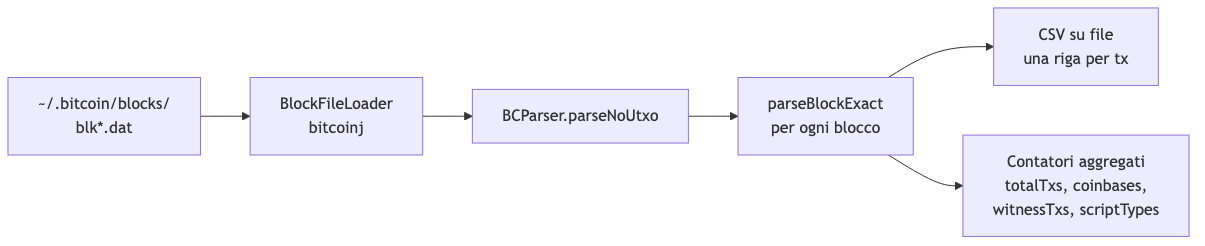
\includegraphics[keepaspectratio,alt={Diagramma Mermaid}]{images/mermaid-lezione-13-lab-script-classification-e-blk-dat-01.png}}
\emph{Fig. --- Pipeline di \texttt{BCParser}: dai file blk.dat al
CSV-like con statistiche aggregate sulla blockchain intera.}

\subsection{Analisi possibili a valle}\label{analisi-possibili-a-valle}

Con un output CSV-like di questo tipo si possono rispondere a domande
come:

\begin{itemize}
\tightlist
\item
  Quanti script di tipo P2PKH vs P2SH vs P2WPKH ci sono nella storia di
  Bitcoin? E come è cambiato il mix nel tempo (segmentando sul
  timestamp)?
\item
  Quante transazioni SegWit sono state fatte dopo l'attivazione di
  agosto 2017?
\item
  Quanti output sono \texttt{PROVABLY\ UNSPENDABLE} (OP\_RETURN)? Che
  payload contengono?
\item
  Quanti indirizzi sono rimasti \texttt{UNKNOWN} --- e quindi usano
  script non-standard (bare multisig, condizioni custom, ecc.)?
\end{itemize}

\begin{callouttip}{Il limite: niente UTXO set}

Il parser scritto in questo laboratorio si chiama \texttt{parseNoUtxo}
per una ragione: non ricostruisce il set degli output non spesi. Per
farlo bisognerebbe, per ogni input, cercare l'output corrispondente
(prevTxHash + prevTxPos) e rimuoverlo dalla collezione degli UTXO vivi.
È fattibile ma richiede molto più lavoro e memoria. Nella versione
attuale ci si limita alle statistiche per transazione.

\end{callouttip}

\begin{center}\rule{0.5\linewidth}{0.5pt}\end{center}

\section{Sintesi operativa}\label{sintesi-operativa-1}

\begin{calloutnote}{Cosa resta in mano dopo il laboratorio}

\begin{itemize}
\tightlist
\item
  Un \textbf{classificatore di script} Bitcoin che riconosce per pattern
  i tipi standard (P2PK, P2PKH, P2SH, P2WPKH, P2WSH, OP\_RETURN, empty)
  e restituisce un codice numerico
\item
  Un \textbf{decodificatore di indirizzo} che applica Base58Check (con
  version 0x00 o 0x05) o Bech32 a seconda del tipo di script
\item
  Un esercizio di estensione per Taproot
  (\texttt{OP\_1\ \textless{}32B\textgreater{}} + Bech32m)
\item
  Conoscenza del formato dei file \texttt{blk*.dat} di Bitcoin Core
\item
  Un \textbf{parser dell'intera blockchain} (\texttt{BCParser}) che
  legge i blk.dat tramite \texttt{BlockFileLoader}, scrive un CSV-like
  con una riga per transazione, e tiene contatori aggregati su tipi di
  script, coinbase, witness e indirizzi non decodificabili
\end{itemize}

\end{calloutnote}

\newpage

\chapter{Bitcoin Security}\label{bitcoin-security}

Il sistema Bitcoin si articola su quattro livelli --- \textbf{Blockchain
Design}, \textbf{P2P Architecture}, \textbf{Consensus} e
\textbf{Transactions} --- ognuno soggetto ad attacchi specifici. La rete
P2P affronta l'Eclipse Attack e l'Approx. Bitcoin Mining; il consenso
subisce il 51\% Attack e il Selfish Mining; le transazioni fronteggiano
il Double Spending e il Malleability Attack. La sicurezza è analizzata
tramite modelli formali come Random Oracle, Nakamoto's Model e Bitcoin
Backbone.

\begin{center}\rule{0.5\linewidth}{0.5pt}\end{center}

\section{Double Spending e Attacco del
51\%}\label{double-spending-e-attacco-del-51}

Il \textbf{Double Spending Attack} consiste nel tentare di spendere lo
stesso bitcoin due volte verso due destinatari diversi. L'approccio
ingenuo --- trasmettere entrambe le transazioni alla rete --- fallisce:
finiscono entrambe nella MemPool, ma un minatore onesto ne includerà
solo una nel blocco successivo, scartando la seconda. Se due minatori le
validano contemporaneamente generando un fork, la Longest Chain Rule ne
renderà valida solo una --- motivo per cui si attendono solitamente 6
conferme.

L'attacco diventa pericoloso in modalità \textbf{stealth}. Il minatore
malevolo: 1. Spende bitcoin sulla catena pubblica per acquistare un bene
(es. una barca) 2. Mina in segreto una catena privata omettendo quella
transazione --- mantenendo il controllo dei bitcoin 3. Quando la catena
privata supera quella pubblica, la trasmette alla rete 4. Per la Longest
Chain Rule, la rete adotta la nuova catena: l'attaccante riottiene i
fondi e mantiene il bene

\pandocbounded{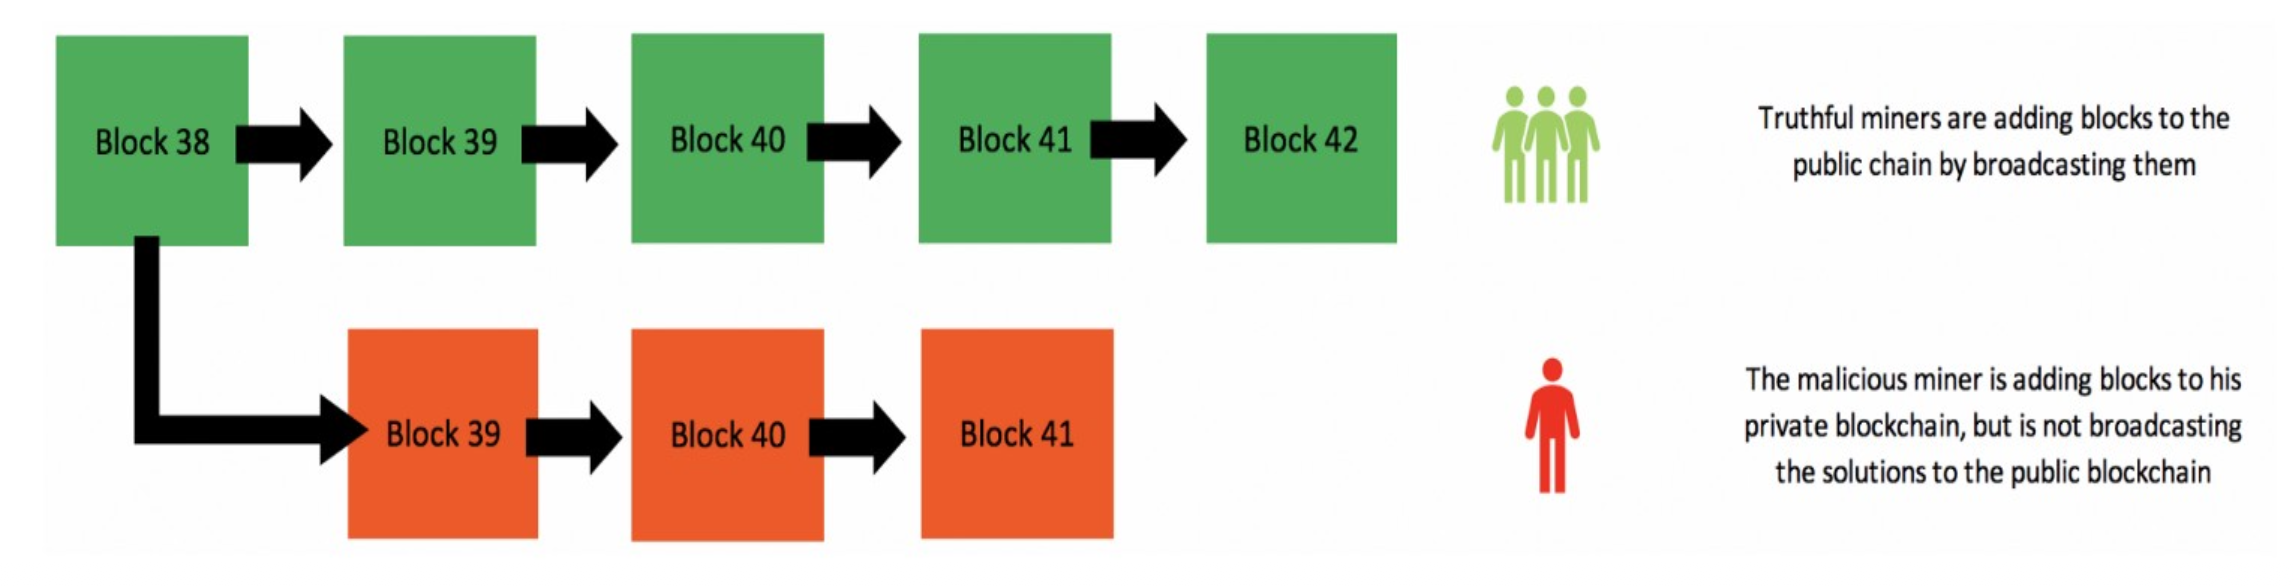
\includegraphics[keepaspectratio]{images/Pasted-image-20260319164820.png}}

Perché l'attacco riesca con regolarità, il minatore deve detenere oltre
il \textbf{50\% dell'hashing power} --- da qui il nome ``51\% Attack''.

\begin{calloutnote}{Il caso GHash.IO (2014)}

La mining pool GHash.IO raggiunse quasi il 50\% della potenza di calcolo
(38,24\%), scatenando il panico nella community. Non subì alcun attacco:
per chi detiene tanto potere è economicamente più conveniente continuare
a minare e incassare i block reward che distruggere il network per
annullare una singola transazione.

\end{calloutnote}

\begin{center}\rule{0.5\linewidth}{0.5pt}\end{center}

\section{Transaction Malleability e il Caso Mt.
Gox}\label{transaction-malleability-e-il-caso-mt.-gox}

La \textbf{Transaction Malleability} permetteva di alterare il
\textbf{TXID} (identificativo) di una transazione senza modificarne gli
effetti reali --- mittente, destinatario e importo restavano invariati,
ma l'ID cambiava. Come se il numero di tracking di un pacco venisse
sostituito in transito.

La vulnerabilità era nell'algoritmo \textbf{ECDSA}: una firma è una
coppia \((r, s)\), ma se \((r, s)\) è valida lo è anche \((r, n-s)\),
dove \(n\) è una costante della curva. Poiché il TXID è l'hash SHA-256
dell'intera transazione (inclusa la firma nello ScriptSig), cambiare la
rappresentazione in \((r, n-s)\) modifica il TXID senza invalidare la
firma logica.

Lo schema di attacco funziona così: Alice invia 50 BTC a Bob, generando
una transazione con TXID = 1234. Bob intercetta la transazione, ne crea
una copia con la firma modificata in \((r, n-s)\) --- stessi input,
stesso output, stessa firma logicamente valida, ma TXID diverso (es.
4567). Ora c'è una gara: entrambe le transazioni finiscono nella
MemPool. Il momento in cui una viene confermata, l'altra viene scartata
come duplicato. Se viene confermata quella di Bob (TXID 4567), Alice non
trova mai il suo TXID originale (1234) sulla blockchain --- e Bob
sostiene di non aver ricevuto nulla, costringendola a un secondo
pagamento.

\begin{calloutnote}{Il fallimento di Mt. Gox (2013–2014)}

Mt. Gox gestiva il 72\% delle transazioni Bitcoin mondiali. Ad aprile
2014 dichiarò bancarotta, avendo perso \textasciitilde744.408 BTC (il
6\% dell'offerta totale, \textasciitilde450 milioni di dollari
dell'epoca). Mt. Gox non usava codifiche di firma standard: alcuni
utenti le ``standardizzavano'' applicando la reverse malleability,
ispirando gli hacker. Gli attaccanti prelevavano fondi, alteravano il
TXID in transito, ricevevano i fondi e --- poiché l'exchange non vedeva
l'ID originale --- rieffettuavano il prelievo.

\end{calloutnote}

La vulnerabilità è stata eliminata con il soft fork \textbf{Segregated
Witness (SegWit)}: i dati della firma vengono spostati in ``witness
data'' separati, e il TXID viene calcolato senza includerli --- la
modifica della firma non può più cambiare l'ID.

\begin{center}\rule{0.5\linewidth}{0.5pt}\end{center}

\section{Attacco Denial of Service}\label{attacco-denial-of-service}

Se un minatore rifiuta di processare le transazioni di un utente
sgradito, quest'ultimo subisce solo un ritardo. La transazione resta
nella MemPool finché qualsiasi altro nodo onesto non propone un blocco
che la include. Non esiste un meccanismo efficace per censurare
permanentemente una transazione in una rete con sufficienti nodi onesti.

\begin{center}\rule{0.5\linewidth}{0.5pt}\end{center}

\section{Attori del Network}\label{attori-del-network}

{\def\LTcaptype{none} % do not increment counter
\begin{longtable}[]{@{}lllll@{}}
\toprule\noalign{}
Tipo di nodo & Wallet & Mining & Blockchain completa & Routing P2P \\
\midrule\noalign{}
\endhead
\bottomrule\noalign{}
\endlastfoot
\textbf{Reference Client (Bitcoin Core)} & Sì & Sì & Sì & Sì \\
\textbf{Full Node} & No & No & Sì & Sì \\
\textbf{Solo Miner} & No & Sì & Sì & Sì \\
\textbf{Lightweight / SPV Wallet} & Sì & No & No & Sì \\
\end{longtable}
}

\begin{center}\rule{0.5\linewidth}{0.5pt}\end{center}

\section{Evoluzione Hardware per il
Mining}\label{evoluzione-hardware-per-il-mining}

Il mining consiste nell'eseguire SHA-256 in loop variando il nonce fino
a ottenere un hash inferiore al target. Il ciclo centrale è
concettualmente semplice:

\begin{verbatim}
while (1)
    HDR[kNoncePos]++;
    if (SHA256(SHA256(HDR)) < (65535 << 208) / DIFFICULTY)
        return;
\end{verbatim}

L'hardware su cui gira questo loop si è evoluto in quattro generazioni,
con guadagni di efficienza enormi ad ogni salto:

{\def\LTcaptype{none} % do not increment counter
\begin{longtable}[]{@{}
  >{\raggedright\arraybackslash}p{(\linewidth - 6\tabcolsep) * \real{0.2500}}
  >{\raggedright\arraybackslash}p{(\linewidth - 6\tabcolsep) * \real{0.2500}}
  >{\raggedright\arraybackslash}p{(\linewidth - 6\tabcolsep) * \real{0.2500}}
  >{\raggedright\arraybackslash}p{(\linewidth - 6\tabcolsep) * \real{0.2500}}@{}}
\toprule\noalign{}
\begin{minipage}[b]{\linewidth}\raggedright
Generazione
\end{minipage} & \begin{minipage}[b]{\linewidth}\raggedright
Periodo
\end{minipage} & \begin{minipage}[b]{\linewidth}\raggedright
Caratteristiche
\end{minipage} & \begin{minipage}[b]{\linewidth}\raggedright
Tempo medio per un blocco
\end{minipage} \\
\midrule\noalign{}
\endhead
\bottomrule\noalign{}
\endlastfoot
\textbf{CPU} & 2009 & Elaborazione sequenziale su core generici &
\textasciitilde139.461 anni (2015, singolo PC) \\
\textbf{GPU} & 2010+ & Alto parallelismo via OpenCL; overclocking
diffuso & \textasciitilde300 anni (100 GPU) \\
\textbf{FPGA} & 2011+ & Schede programmabili via Verilog; ottime per
operazioni bitwise & \textasciitilde25 anni \\
\textbf{ASIC} & 2013+ & Chip dedicati esclusivamente a SHA-256 (es.
TerraMiner 4: 2 TH/s a \$3.500) & Secondi/minuti \\
\end{longtable}
}

\begin{center}\rule{0.5\linewidth}{0.5pt}\end{center}

\section{Solo Mining vs Mining Pool}\label{solo-mining-vs-mining-pool}

Il \textbf{solo mining} segue una distribuzione di Poisson con alta
varianza: nel 2014, con 1700 GH/s, l'attesa media per un blocco era
oltre 3 anni. Si accumula stress e spese senza entrate garantite.

La deviazione standard è alta per costruzione: se in un mese ci si
aspetta di trovare 4 blocchi, la deviazione standard è \(\sqrt{4} = 2\).
Significa che alcuni mesi se ne trovano 6, altri 2, altri 0. Oltre
all'incertezza economica, il solo mining introduce un problema di
fiducia: il miner non può verificare in modo indipendente se il proprio
hardware funzioni correttamente, né se gli altri miner stiano barando
per ottenere una quota sproporzionata dei premi --- e in effetti i miner
\emph{possono} imbrogliarsi a vicenda. Questo è uno dei motivi
principali che ha spinto verso le mining pool.

Le \textbf{Mining Pool} aggregano i minatori riducendo la varianza in
cambio di entrate più piccole ma costanti. Un \emph{Pool Manager}
centrale distribuisce il lavoro, raccoglie le soluzioni e redistribuisce
i premi trattenendo una fee. Per verificare che i minatori stiano
davvero lavorando, questi inviano \textbf{shares}: blocchi ``quasi
validi'' con una difficoltà ridotta rispetto alla rete, che fungono da
prova probabilistica del lavoro svolto.

\subsection{Metodi di Pagamento}\label{metodi-di-pagamento}

La scelta del metodo di pagamento è il cuore del rapporto economico tra
pool e miner: determina chi si fa carico del rischio della varianza e
come viene scoraggiato il comportamento opportunistico. Esistono tre
schemi principali, con varianti ibride usate dalle pool moderne.

\subsubsection{Pay Per Share (PPS) e
FPPS}\label{pay-per-share-pps-e-fpps}

Nel modello \textbf{PPS} (\emph{Pay Per Share}), il miner viene pagato
per ogni share valida inviata, indipendentemente dal fatto che la pool
trovi effettivamente un blocco. Il pagamento è deterministico: se la
difficoltà della rete è \(D\) e la difficoltà delle share è \(d\), ogni
share vale esattamente \(\frac{d}{D} \cdot \text{block\_reward}\). La
pool si assume interamente il rischio della varianza --- in settimane
sfortuna, pagherà i miner anche senza ricavare premi.

\textbf{FPPS} (\emph{Fully Pay Per Share}) è la variante estesa: oltre
al block reward, include nella quota per share anche le
\textbf{transaction fees} del blocco (che in PPS puro vengono spesso
trattenute dall'operatore). FPPS è quindi più generoso per il miner ma
richiede una fee operativa più alta.

\begin{calloutwarning}{Incentivo perverso del PPS}

Poiché il miner viene pagato a prescindere, non ha alcun incentivo a
trasmettere immediatamente un blocco valido trovato --- potrebbe
teoricamente scartarlo per massimizzare le proprie share senza
contribuire alla catena. Nella pratica questo comportamento è raro
perché degenera nella loss di reputazione e nella rimozione dalla pool.

\end{calloutwarning}

\subsubsection{Pay Per Last N Shares
(PPLNS)}\label{pay-per-last-n-shares-pplns}

Nel modello \textbf{PPLNS}, la ricompensa viene distribuita solo quando
la pool trova un blocco, e viene ripartita in proporzione alle share che
ciascun miner ha inviato nell'ultima finestra di \(N\) share. Il
parametro \(N\) è scelto dall'operatore: una finestra piccola premia i
miner più recenti; una finestra grande diluisce il contributo nel tempo.

L'effetto principale è che il miner si espone alla stessa varianza della
pool: se la pool trova molti blocchi in rapida successione, guadagna
molto; se è sfortunata, guadagna poco. In compenso, la fee è bassa
perché l'operatore non anticipa pagamenti.

\begin{callouttip}{PPLNS scoraggia il pool hopping}

Il \textbf{pool hopping} è la strategia di un miner opportunista che si
unisce a una pool all'inizio di un round (quando le share accumulate
sono poche e la sua quota relativa è alta) per poi passare a un'altra
pool verso la fine. Con PPLNS la finestra scorrente penalizza chi entra
tardi o è intermittente: le sue share recenti hanno peso minore rispetto
a chi contribuisce stabilmente. Questo rende PPLNS resistente al pool
hopping.

\end{callouttip}

\subsubsection{Pay Proportional}\label{pay-proportional}

Nel modello \textbf{proporzionale}, la ricompensa di ogni blocco trovato
viene divisa tra i miner in proporzione alle share inviate \emph{durante
quel round} (cioè dall'ultimo blocco trovato dalla pool al blocco
corrente). A differenza di PPLNS non c'è finestra scorrevole: si azzera
ad ogni blocco.

Questo schema è vulnerabile al pool hopping in modo ancora più diretto:
un miner che entra a inizio round (quando poche share sono state
accumulate) ha una quota percentuale molto alta. Man mano che il round
si allunga, nuovi miner entrano e la quota si diluisce --- conviene
quindi abbandonare i round lunghi. Per questo motivo il Pay Proportional
puro è stato quasi completamente abbandonato in favore di PPLNS.

\subsubsection{Confronto riassuntivo}\label{confronto-riassuntivo}

{\def\LTcaptype{none} % do not increment counter
\begin{longtable}[]{@{}
  >{\raggedright\arraybackslash}p{(\linewidth - 8\tabcolsep) * \real{0.2000}}
  >{\raggedright\arraybackslash}p{(\linewidth - 8\tabcolsep) * \real{0.2000}}
  >{\raggedright\arraybackslash}p{(\linewidth - 8\tabcolsep) * \real{0.2000}}
  >{\raggedright\arraybackslash}p{(\linewidth - 8\tabcolsep) * \real{0.2000}}
  >{\raggedright\arraybackslash}p{(\linewidth - 8\tabcolsep) * \real{0.2000}}@{}}
\toprule\noalign{}
\begin{minipage}[b]{\linewidth}\raggedright
Metodo
\end{minipage} & \begin{minipage}[b]{\linewidth}\raggedright
Chi porta il rischio varianza
\end{minipage} & \begin{minipage}[b]{\linewidth}\raggedright
Vulnerabile al pool hopping
\end{minipage} & \begin{minipage}[b]{\linewidth}\raggedright
Fee tipica
\end{minipage} & \begin{minipage}[b]{\linewidth}\raggedright
Transaction fees incluse
\end{minipage} \\
\midrule\noalign{}
\endhead
\bottomrule\noalign{}
\endlastfoot
\textbf{PPS} & Operatore della pool & No & Alta & No \\
\textbf{FPPS} & Operatore della pool & No & Alta & Sì \\
\textbf{PPLNS} & Il miner & Parzialmente (finestra scorrevole lo riduce)
& Bassa & Dipende dalla pool \\
\textbf{Pay Proportional} & Il miner & Sì (molto vulnerabile) & Bassa &
Dipende dalla pool \\
\end{longtable}
}

\begin{calloutwarning}{Mining Pool Decentralizzate (es. P2Pool, dal 2011)}

Non richiedono un operatore fidato. I miner costruiscono in parallelo
una \textbf{sharechain} --- una blockchain privata con difficoltà
ridotta (\textasciitilde un blocco ogni 30 secondi) --- agganciata
all'ultimo blocco Bitcoin. Ogni share è scritta sulla sharechain e
registra la quota di ricompensa spettante. Quando si trova un blocco
Bitcoin valido, i pagamenti vengono processati sulla rete principale
tramite \emph{merge mining}. L'auditability totale impedisce truffe
interne.

\end{calloutwarning}

\subsection{Top Mining Pool (2025)}\label{top-mining-pool-2025}

{\def\LTcaptype{none} % do not increment counter
\begin{longtable}[]{@{}llll@{}}
\toprule\noalign{}
Pool & Fee & Hashrate & Metodo \\
\midrule\noalign{}
\endhead
\bottomrule\noalign{}
\endlastfoot
Foundry USA & 2\% PPLNS / 4\% PPS & 231,5 EH/s & FPPS \\
BTC.com & 1,38\% & 161,44 EH/s & Advanced FPPS \\
Antpool & 0\% PPLNS / 4\% PPS+ & 30,5 EH/s & PPLNS, PPS+ \\
F2Pool & 2,5\% & 25,81 EH/s & PPS+ \\
Binance & 2,5\% & 23,86 EH/s & FPPS, PPS+, PPS \\
Poolin & 2,5\% & 23,59 EH/s & FPPS \\
ViaBTC & 2\% PPLNS / 4\% PPS & 20,32 EH/s & PPLNS, PPS \\
\end{longtable}
}

Le pool sono nate nel 2010 (era GPU) e già nel 2014 raccoglievano il
90\% dell'hashrate globale. I protocolli standardizzati odierni
facilitano lo spostamento dei miner tra pool diverse.

\newpage

\chapter{Advanced Bitcoin Scripts e SPV
Clients}\label{advanced-bitcoin-scripts-e-spv-clients}

Tre costrutti avanzati di Bitcoin --- \textbf{multisignature},
\textbf{hash lock} e \textbf{time lock} --- sono alla base della
Lightning Network, la principale soluzione di scalabilità per Bitcoin.

\begin{center}\rule{0.5\linewidth}{0.5pt}\end{center}

\section{Multisignature (Multisig)}\label{multisignature-multisig}

In un protocollo multi-firma, un gruppo di firmatari autorizza
collettivamente una transazione; la verifica avviene tramite le chiavi
pubbliche di tutti i partecipanti. L'approccio ingenuo concatena le
firme individuali, ma la dimensione cresce linearmente con il numero di
firmatari. L'ideale sarebbe una dimensione fissa indipendente dal numero
di partecipanti.
\pandocbounded{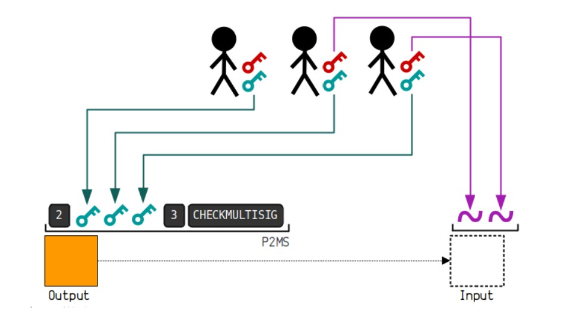
\includegraphics[keepaspectratio]{images/Pasted-image-20260407113044.png}}
Bitcoin ha adottato inizialmente la soluzione più semplice con
\textbf{ECDSA}: firme multiple separate, non aggregate. Le \textbf{firme
Schnorr}, che permettono l'aggregazione, sono state introdotte solo in
seguito con il protocollo \textbf{Taproot}.

Un indirizzo multisig accoppia un indirizzo Bitcoin a un locking script
che richiede \textbf{M} firme valide su \textbf{N} chiavi pubbliche
associate.

\subsection{Script Multisig}\label{script-multisig}

\textbf{Locking script} M-of-N:

\begin{verbatim}
M <PubKey1> … <PubKeyN> N OP_CHECKMULTISIG
\end{verbatim}

\textbf{Unlocking script} (qualsiasi combinazione valida di M firme):

\begin{verbatim}
<Signature 1> … <Signature M>
\end{verbatim}

Esempio 2-of-3 con Alice, Bob e Judy: - Locking:
\texttt{2\ \textless{}PkA\textgreater{}\ \textless{}PkB\textgreater{}\ \textless{}PkC\textgreater{}\ 3\ OP\_CHECKMULTISIG}
- Unlocking valido:
\texttt{\textless{}Sig\ A\textgreater{}\ \textless{}Sig\ C\textgreater{}}
--- qualsiasi due delle tre

\subsection{Casi d'uso}\label{casi-duso}

{\def\LTcaptype{none} % do not increment counter
\begin{longtable}[]{@{}
  >{\raggedright\arraybackslash}p{(\linewidth - 2\tabcolsep) * \real{0.5000}}
  >{\raggedright\arraybackslash}p{(\linewidth - 2\tabcolsep) * \real{0.5000}}@{}}
\toprule\noalign{}
\begin{minipage}[b]{\linewidth}\raggedright
Schema
\end{minipage} & \begin{minipage}[b]{\linewidth}\raggedright
Caso d'uso
\end{minipage} \\
\midrule\noalign{}
\endhead
\bottomrule\noalign{}
\endlastfoot
\textbf{1-of-2} & Conto corrente coniugale per piccole spese --- basta
la firma di uno \\
\textbf{2-of-2} & Conto risparmio --- entrambi devono approvare \\
\textbf{2-of-2} & Wallet con autenticazione a due fattori (laptop +
smartphone) --- un trojan sul telefono non basta per rubare i fondi \\
\textbf{2-of-2} & Blocco fondante della Lightning Network \\
\textbf{2-of-3} & Conto risparmio genitore-figlio --- il figlio non può
prelevare senza il consenso di un genitore \\
\textbf{2-of-3} & Escrow trustless tra compratore e venditore con
arbitro \\
\end{longtable}
}

\begin{center}\rule{0.5\linewidth}{0.5pt}\end{center}

\section{Transazioni Escrow}\label{transazioni-escrow}

Alice vuole acquistare un libro raro da Bob, ma vivono in città diverse
e non si fidano l'uno dell'altro: Alice non vuole pagare prima di
ricevere il libro, Bob non vuole spedire prima di essere pagato.

La soluzione è una \textbf{transazione escrow 2-of-3} con Judy come
arbitro neutrale. Alice crea la transazione multisig con una chiave
pubblica ciascuno per Alice, Bob e Judy, e la pubblica sulla blockchain.
I fondi entrano in una sorta di ``limbo'': nessuno può muoverli da solo,
servono sempre due firme. L'escrow fallisce solo se Judy collude
esplicitamente con una delle parti.

\begin{callouttip}{I tre scenari possibili}

\textbf{2a --- Tutto ok}: Alice riceve il libro. Alice e Bob firmano
insieme per rilasciare i fondi a Bob. Judy non viene coinvolta. Servono
due transazioni: una per depositare nell'escrow, una per pagare Bob.

\textbf{2b --- Alice riceve ma rifiuta di pagare}: Bob fornisce a Judy
la prova di spedizione. Bob e Judy firmano insieme per inviare i fondi a
Bob.

\textbf{2c --- Bob non spedisce}: Alice dimostra a Judy di non aver
ricevuto nulla. Alice e Judy firmano insieme per restituire i fondi ad
Alice.

\end{callouttip}

\begin{center}\rule{0.5\linewidth}{0.5pt}\end{center}

\section{Pay-To-Script-Hash (P2SH)}\label{pay-to-script-hash-p2sh}

Gli script multisig sono scomodi in pratica. Se un cliente deve pagare
un'azienda con un multisig 2-of-5, l'azienda deve trasmettere l'intero
script al cliente, che ha bisogno di un wallet speciale per costruirlo.
La transazione risultante è cinque volte più grande del normale: fee più
alte (a carico del mittente), script troppo lungo per un QR code, e
l'intero script resta in RAM nel set UTXO di ogni full node finché non
viene speso.

\pandocbounded{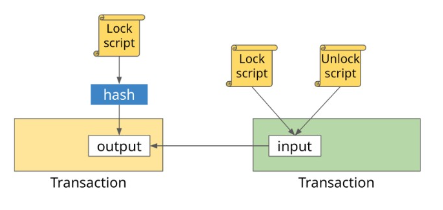
\includegraphics[keepaspectratio]{images/Pasted-image-20260407113120.png}}

\textbf{P2SH} (BIP-16, gennaio 2012) risolve il problema: il
destinatario del pagamento è identificato dall'\textbf{hash dello
script}, non dallo script stesso.

{\def\LTcaptype{none} % do not increment counter
\begin{longtable}[]{@{}
  >{\raggedright\arraybackslash}p{(\linewidth - 4\tabcolsep) * \real{0.3333}}
  >{\raggedright\arraybackslash}p{(\linewidth - 4\tabcolsep) * \real{0.3333}}
  >{\raggedright\arraybackslash}p{(\linewidth - 4\tabcolsep) * \real{0.3333}}@{}}
\toprule\noalign{}
\begin{minipage}[b]{\linewidth}\raggedright
\end{minipage} & \begin{minipage}[b]{\linewidth}\raggedright
Locking script
\end{minipage} & \begin{minipage}[b]{\linewidth}\raggedright
Unlocking script
\end{minipage} \\
\midrule\noalign{}
\endhead
\bottomrule\noalign{}
\endlastfoot
\textbf{Multisig classico} &
\texttt{OP\_1\ \textless{}PK1\textgreater{}\ \textless{}PK2\textgreater{}\ OP\_2\ OP\_CHECKMULTISIG}
& \texttt{OP\_0\ \textless{}Sig1\textgreater{}} \\
\textbf{P2SH} &
\texttt{OP\_HASH160\ \textless{}RedeemScriptHash\textgreater{}\ OP\_EQUAL}
&
\texttt{OP\_0\ \textless{}Sig1\textgreater{}\ \textless{}Sig2\textgreater{}\ \textbackslash{}\textbar{}\ \textless{}OP\_2\ \textless{}PK1\textgreater{}\ \textless{}PK2\textgreater{}\ \textless{}PK3\textgreater{}\ OP\_3\ OP\_CHECKMULTISIG\textgreater{}} \\
\end{longtable}
}

Per riscattare un P2SH l'utente presenta: la firma richiesta + il
\emph{Redeem Script} originale in chiaro, che hashato deve coincidere
con l'hash nel locking script.

\begin{callouttip}{Il vantaggio chiave del P2SH}

Il P2SH sposta tutti gli oneri \textbf{dal mittente al destinatario}: -
La complessità di costruire lo script passa al destinatario - Le fee
aggiuntive per lo script lungo le paga il destinatario (al momento della
spesa), non il mittente - Lo script lungo non occupa RAM nell'UTXO set
ora, ma viene registrato sulla blockchain solo quando viene speso
(nell'input) - Gli script vengono codificati come normali indirizzi:
qualsiasi wallet semplice può pagare

\end{callouttip}

\begin{center}\rule{0.5\linewidth}{0.5pt}\end{center}

\section{Hash-Time Locked Contracts
(HTLC)}\label{hash-time-locked-contracts-htlc}

Un HTLC combina due meccanismi:

\begin{calloutdefinition}{HTLC}

\begin{itemize}
\tightlist
\item
  \textbf{Hash Lock}: l'hash di un segreto è pubblicato nello script. I
  fondi si sbloccano solo se il destinatario rivela pubblicamente il
  segreto originale.
\item
  \textbf{Time Lock}: condizione di fallback --- se entro un timeout
  prestabilito il segreto non viene rivelato, i fondi tornano al
  mittente.
\end{itemize}

\end{calloutdefinition}

Gli HTLC sono usati nei \textbf{payment channel} (Lightning Network) e
negli \textbf{Atomic Swap}.

\subsection{Atomic Swap}\label{atomic-swap}

Un Atomic Swap permette di scambiare criptovalute su blockchain diverse
in modo \emph{trustless}, senza exchange centralizzati. Il problema
classico: chi invia i fondi per primo rischia che la controparte non
adempia. L'HTLC risolve sincronizzando i due lati dello scambio.

\textbf{Esempio}: Alice ha BTC e vuole ZEN di Bob.

\begin{enumerate}
\def\labelenumi{\arabic{enumi}.}
\tightlist
\item
  Alice genera un segreto \texttt{s}, ne calcola \texttt{H(s)} e crea un
  HTLC sulla blockchain Bitcoin bloccando 1 BTC: Bob può riscattarli
  rivelando \texttt{s}, oppure dopo 24 ore i fondi tornano ad Alice.
  Alice invia \texttt{H(s)} a Bob.
\item
  Bob crea un HTLC identico sulla blockchain ZEN bloccando 200 ZEN con
  lo stesso \texttt{H(s)} e un timelock di 24 ore.
\item
  Alice usa \texttt{s} per sbloccare l'HTLC di Bob sulla rete ZEN e
  incassare i 200 ZEN --- operazione pubblica e registrata sulla
  blockchain.
\item
  Bob legge \texttt{s} dalla blockchain ZEN e lo usa per sbloccare
  l'HTLC di Alice su Bitcoin, incassando 1 BTC.
\end{enumerate}

L'hashlock sincronizza lo scambio; il timelock garantisce che nessuno
perda i fondi se la controparte sparisce.

\begin{center}\rule{0.5\linewidth}{0.5pt}\end{center}

\section{Data Registering e Proof of
Burn}\label{data-registering-e-proof-of-burn}

La blockchain può fungere da \textbf{registro notarile}: si calcola
l'hash di un documento e lo si registra on-chain per provare l'esistenza
di quel file in una data specifica.

Il metodo originale era simulare un pagamento verso un indirizzo falso
(nessuno ha la chiave privata corrispondente) usando 20 byte liberi come
campo dati. Il problema: quell'UTXO non può mai essere rimosso dalla RAM
dei full node --- \textbf{data pollution}.

\textbf{OP\_RETURN} (introdotto dopo il 2013 come compromesso)
standardizza la registrazione:

\begin{verbatim}
OP_RETURN <Data>
\end{verbatim}

L'output è esplicitamente non spendibile: i coin associati vengono
distrutti, ma l'entry non entra nell'UTXO set e non inquina la RAM. Si
usa in due modi: - Solo per registrare dati (senza bruciare coin
significativi) - \textbf{Proof of Burn}: distruggere deliberatamente
coin in modo verificabile

\begin{calloutnote}{Usi della Proof of Burn}

\begin{itemize}
\tightlist
\item
  \textbf{Bootstrap di nuove criptovalute}: gli utenti bruciano BTC per
  ottenere token della nuova chain, distribuendo la supply in modo
  decentralizzato
\item
  \textbf{Consenso alternativo}: si vince la ``lotteria dei blocchi''
  bruciando coin invece di consumare energia (come nella PoW). Il
  bilanciamento matematico tra coin bruciati e ricompense è però
  difficile da implementare correttamente.
\end{itemize}

\end{calloutnote}

\begin{center}\rule{0.5\linewidth}{0.5pt}\end{center}

\section{Simplified Payment Verification
(SPV)}\label{simplified-payment-verification-spv}

Scaricare l'intera blockchain (\textgreater649 GB ad aprile 2025) non è
pratico su smartphone. I \textbf{client SPV} (o \emph{lightweight
client}) scaricano solo gli \textbf{header dei blocchi} --- circa 80
byte ciascuno, mille volte più leggeri del blocco completo --- e sono
interessati solo alle transazioni che riguardano gli indirizzi nel
proprio wallet.

La sicurezza è mantenuta su due livelli: - L'header contiene il
\textbf{nonce}: si può verificare che la Proof of Work sia stata
completata - La validità di una transazione si verifica tramite
\textbf{Merkle proof}: il full node invia il ramo del Merkle Tree che
collega la transazione alla Merkle Root nell'header. L'SPV ricalcola
ricorsivamente gli hash dal basso verso l'alto e confronta il risultato
con la radice --- se coincide, la transazione è autentica.

\subsection{Bloom Filter e Privacy}\label{bloom-filter-e-privacy}

Richiedere transazioni specifiche per indirizzo rivelerebbe al full node
quali indirizzi appartengono all'utente. Per proteggere la privacy,
l'SPV invia al full node un \textbf{Bloom filter} costruito sugli
indirizzi del wallet (OR bit a bit degli hash di ogni indirizzo).

Il full node testa ogni output di ogni transazione contro il filtro: -
Se tutti gli hash restituiscono un bit a 1 → la transazione è
\emph{probabilmente} rilevante → viene inviata all'SPV - Se anche un
solo hash restituisce uno 0 → la transazione è \emph{certamente}
irrilevante → viene ignorata

I falsi positivi sono accettati deliberatamente: nascondono quali
indirizzi interessano davvero all'SPV (privacy) e rimangono comunque
pochi (efficienza di banda).

\begin{center}\rule{0.5\linewidth}{0.5pt}\end{center}

\section{Bitcoin Protocol Stack e Rete
P2P}\label{bitcoin-protocol-stack-e-rete-p2p}

{\def\LTcaptype{none} % do not increment counter
\begin{longtable}[]{@{}
  >{\raggedright\arraybackslash}p{(\linewidth - 2\tabcolsep) * \real{0.5000}}
  >{\raggedright\arraybackslash}p{(\linewidth - 2\tabcolsep) * \real{0.5000}}@{}}
\toprule\noalign{}
\begin{minipage}[b]{\linewidth}\raggedright
Livello
\end{minipage} & \begin{minipage}[b]{\linewidth}\raggedright
Descrizione
\end{minipage} \\
\midrule\noalign{}
\endhead
\bottomrule\noalign{}
\endlastfoot
\textbf{Application layer} & Applicazioni user-facing che usano la
blockchain \\
\textbf{Transaction layer} & Script e logica di validità delle
transazioni \\
\textbf{Consensus layer} & Algoritmi per l'accordo sull'incorporazione
delle transazioni (es. PoW) \\
\textbf{Network (P2P) layer} & Broadcasting dei dati tra i nodi \\
\end{longtable}
}

La rete P2P è \textbf{non strutturata}: chiunque può connettersi. Di
default ogni nodo mantiene 117 connessioni TCP in uscita e accetta fino
a 8 in entrata sulla porta 8333, senza autenticazione né cifratura.
\pandocbounded{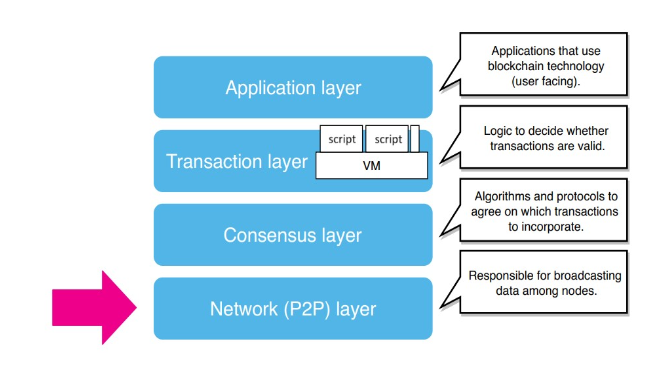
\includegraphics[keepaspectratio]{images/Pasted-image-20260407113308.png}}

\subsection{Bootstrap e Peer
Discovery}\label{bootstrap-e-peer-discovery}

Un nodo nuovo deve prima trovare qualcuno con cui parlare. I metodi in
ordine di preferenza: 1. \textbf{Seed address hard-coded} nel client ---
nodi stabili con IP statici 2. \textbf{DNS bootstrap} --- server DNS
dedicati che restituiscono liste di IP 3. \textbf{Forum e chat} ---
fallback manuale se tutto il resto fallisce

Una volta connesso, il nodo ricorda gli indirizzi dei peer con cui ha
comunicato con successo: al riavvio può riconnettersi rapidamente senza
ripartire da zero.

Per scoprire ulteriori peer, il nodo invia messaggi \texttt{GETADDR} ai
vicini, che rispondono con messaggi \texttt{ADDR} contenenti liste di
IP. Il nuovo nodo annuncia anche se stesso inviando un \texttt{ADDR} con
il proprio IP, che i vicini propagano ai loro vicini.

\subsection{Handshake}\label{handshake}

All'apertura di una connessione, i nodi si scambiano un messaggio
\texttt{VERSION} che contiene tra l'altro il campo \textbf{bestHeight}
--- l'altezza corrente della blockchain del nodo. Se un nodo ha una
catena più corta di quella del vicino, richiede i blocchi mancanti.
\pandocbounded{
\includegraphics[keepaspectratio]{images/Pasted-image-20260407113353.png}}
\#\#\# Gossip Protocol e Propagazione

La propagazione di transazioni e blocchi avviene tramite \textbf{gossip}
(\emph{any-to-all}): ogni nodo propaga ai propri vicini ciò che riceve.

Il flusso standard per una transazione o un blocco:

\begin{enumerate}
\def\labelenumi{\arabic{enumi}.}
\tightlist
\item
  \textbf{\texttt{INV}} --- messaggio di annuncio: il nodo invia ai
  vicini l'hash della transazione/blocco (non il contenuto). È una
  notifica, non un invio.
\item
  \textbf{\texttt{GETDATA}} --- i vicini che non hanno già quel dato
  richiedono il contenuto completo.
\item
  \textbf{\texttt{BLOCK} / \texttt{TRANSACTION}} --- il nodo invia il
  dato effettivo.
\end{enumerate}

\begin{callouttip}{Minimizzare il consumo di banda}

Se lo stesso hash arriva da più peer contemporaneamente, il nodo invia
\texttt{GETDATA} a \textbf{uno solo} di essi. Questo evita di scaricare
lo stesso dato più volte.

\end{callouttip}

\textbf{Unsolicited Block Push}: quando un miner trova un blocco, sa con
certezza di essere l'unico ad averlo. Salta il passaggio \texttt{INV} e
invia direttamente il blocco ai vicini --- ogni secondo conta per non
perdere il vantaggio competitivo.

\textbf{GETBLOCK}: un nodo che si è disconnesso o si avvia per la prima
volta deve sincronizzarsi. Chiede al vicino la sua visione locale della
blockchain; il vicino risponde con gli hash dei blocchi a varie altezze.
Il nodo trova il primo hash in comune con la propria catena e richiede i
blocchi successivi tramite \texttt{GETDATA}. Il processo è iterativo:
dopo aver scaricato un batch, invia un nuovo \texttt{GETBLOCK} fino a
essere aggiornato.

\subsection{Protezione contro il DoS}\label{protezione-contro-il-dos}

Nodi malevoli potrebbero inondare la rete con oggetti invalidi,
saturando la banda. La protezione è integrata nel protocollo per design:

\begin{itemize}
\tightlist
\item
  Un nodo invia un messaggio \texttt{INV} ai vicini \textbf{solo dopo
  aver validato} il blocco o la transazione (firma valida, UTXO valido)
\item
  Ogni nodo mantiene uno \textbf{score di reputazione} per ciascun peer
\item
  Se un peer si comporta male (es. invia transazioni con firme
  invalide), il suo score viene degradato
\item
  Sotto una certa soglia, il peer viene disconnesso
\end{itemize}

\newpage

\chapter{Lezione 16 --- Lightning network of
Bitcoin}\label{lezione-16-lightning-network-of-bitcoin}

\section{Il Trilemma della
Blockchain}\label{il-trilemma-della-blockchain}

Prima di capire perché esiste la Lightning Network, occorre capire il
problema che intende risolvere. Vitalik Buterin ha formalizzato
l'osservazione che i sistemi blockchain tendono a soddisfare al massimo
due delle tre proprietà desiderabili simultaneamente.

\begin{calloutdefinition}{Trilemma della Blockchain (Buterin)}

Un sistema blockchain può soddisfare al massimo due delle seguenti tre
proprietà: \textbf{decentralizzazione} (nessun punto di controllo
centrale, resistenza alla censura), \textbf{scalabilità} (capacità di
gestire un numero crescente di transazioni per unità di tempo),
\textbf{sicurezza} (capacità di operare correttamente e difendersi dagli
attacchi).

\end{calloutdefinition}

Concretamente, i sistemi esistenti si posizionano in modo diverso su
questo triangolo. Bitcoin ed Ethereum privilegiano sicurezza e
decentralizzazione, ma non scalano --- Bitcoin elabora circa 7
transazioni al secondo a livello globale, contro le 65.000 di Visa.
Hyperledger e Ripple sono sicuri e scalabili, ma centralizzati: un
numero ristretto di nodi controlla la rete, con minima resistenza alla
censura. IOTA era scalabile e decentralizzato, ma usava un Proof-of-Work
leggero che ne comprometteva la sicurezza.

Il problema è quantitativamente serio. Con blocchi da 1 MB (4 MB dal
2017 con SegWit) e transazioni medie da 250 byte, Bitcoin può contenere
circa 400 transazioni per blocco, che a un blocco ogni 10 minuti danno 7
TPS. La conferma richiede 6 blocchi per considerarsi definitiva, quindi
circa un'ora di attesa. Non c'è confronto con i sistemi di pagamento
tradizionali.

\subsection{Perché le soluzioni on-chain non
bastano}\label{perchuxe9-le-soluzioni-on-chain-non-bastano}

La prima risposta intuitiva è: aumentiamo la dimensione del blocco.
Bitcoin Cash ha fatto esattamente questo, portando prima a 8 MB e poi a
32 MB in un hard fork. Il problema è che per raggiungere la stessa
capacità di Visa servirebbero blocchi da 8 GB --- non è un errore di
battitura. I nodi dovrebbero archiviare circa 400 TB di dati generati
ogni anno e disporre di 120 megabit/sec di banda. Il risultato
inevitabile è che solo un piccolo numero di nodi con risorse molto
elevate potrebbe partecipare, aumentando la centralizzazione e riducendo
la sicurezza.

Aumentare il tasso di produzione dei blocchi introduce un altro
problema: più fork concorrenti, con conseguente riduzione della
sicurezza complessiva. Il Proof-of-Stake e i protocolli di consenso
leggeri risolvono il problema energetico e scalano meglio, ma spesso non
sono davvero decentralizzati in pratica, e tendono a favorire chi è già
ricco.

\begin{center}\rule{0.5\linewidth}{0.5pt}\end{center}

\section{L'Idea dei Canali di Pagamento
Off-Chain}\label{lidea-dei-canali-di-pagamento-off-chain}

L'intuizione chiave che sblocca il problema è questa: non è necessario
che ogni transazione finisca sulla blockchain. La blockchain è lenta e
cara da usare perché richiede consenso globale tra tutti i nodi --- ma
il consenso globale è necessario solo per il regolamento finale dei
fondi, non per ogni singolo pagamento intermedio.

\begin{callouttip}{Intuizione chiave}

Spostare la maggior parte delle transazioni \emph{fuori} dalla
blockchain, usando la catena solo per aprire e chiudere i canali di
pagamento. In mezzo, le parti si scambiano ``cambiali'' (promissory
notes) off-chain, a velocità di rete.

\end{callouttip}

L'analogia della slide è illuminante: immaginate un cliente al bar che
dà la carta di credito al barista all'inizio della serata. Il barista
segna ogni drink su un conto ma non addebita la carta ad ogni giro,
evitando le commissioni. Alla fine della serata regola tutto con
un'unica transazione. Il barista non rischia niente perché ha la carta
in mano come garanzia; se il cliente sparisce, può addebitarla. Nella
Lightning Network, la ``carta di credito'' è il deposito in un indirizzo
multifirma sulla blockchain, e le ``cambiali'' sono transazioni Bitcoin
firmate ma non ancora trasmesse in rete.

I canali di pagamento off-chain sono quindi:

\begin{itemize}
\tightlist
\item
  \textbf{trustless}: non richiedono fiducia reciproca tra le parti,
  perché la blockchain funge da arbitro
\item
  \textbf{decentralizzati}: costruiti sopra l'infrastruttura di Bitcoin,
  senza hard fork
\item
  \textbf{istantanei}: le transazioni avvengono alla velocità della rete
  peer-to-peer, non ai ritmi della blockchain
\item
  \textbf{ad alto volume}: potenzialmente illimitati in numero di
  transazioni per canale
\end{itemize}

La tipologia base è \textbf{unidirezionale} (una parte paga sempre
l'altra), ma le estensioni più importanti sono i \textbf{canali
bidirezionali} e la \textbf{composizione di canali} --- che insieme
costituiscono la Lightning Network vera e propria.

\begin{center}\rule{0.5\linewidth}{0.5pt}\end{center}

\section{Il Protocollo Lightning
Network}\label{il-protocollo-lightning-network}

La Lightning Network è un protocollo di livello 2 proposto da Joseph
Poon e Thaddeus Dryja nel 2015. Tecnicamente si basa su tre operazioni
fondamentali per ogni canale: apertura, impegni off-chain e chiusura.

\subsection{Apertura del Canale: la Funding
Transaction}\label{apertura-del-canale-la-funding-transaction}

A livello tecnico, un canale di pagamento è un \textbf{indirizzo
multifirma 2-di-2} --- per spendere i fondi in quell'indirizzo servono
le firme di entrambe le parti (Alice e Bob), esattamente come un conto
bancario cointestato che richiede due firme per i prelievi.

Per aprire il canale, Alice crea una \textbf{funding transaction} che
invia i suoi bitcoin all'indirizzo multifirma. Questa è l'unica
transazione che deve comparire sulla blockchain durante l'intera vita
del canale. La struttura è:

\begin{verbatim}
Funding Transaction:
  Input:  Indirizzo di Alice
  Output: Indirizzo multifirma Alice+Bob
  Importo: 100K satoshi
\end{verbatim}

I fondi restano ``in escrow'' nell'indirizzo condiviso finché il canale
non viene chiuso.

\subsection{Impegni Off-Chain: le Commitment
Transactions}\label{impegni-off-chain-le-commitment-transactions}

Una volta aperto il canale, Alice e Bob si scambiano \textbf{commitment
transactions} --- transazioni Bitcoin valide che ridistribuiscono i
fondi del multifirma tra i due, ma che \emph{non vengono trasmesse}
sulla blockchain. Rimangono conservate localmente da ciascuna delle
parti.

Ogni commitment transaction ha questa struttura:

\begin{verbatim}
Commitment Transaction N:
  Input:  Indirizzo multifirma Alice+Bob
  Output: Alice → importo_A satoshi
  Output: Bob  → importo_B satoshi
\end{verbatim}

La transazione deve essere firmata da entrambi. La sequenza tipica è:
Alice firma la transazione e la invia a Bob, che la controfirma e la
conserva (e viceversa). Così entrambi hanno in mano un documento valido
che, se trasmesso, si traduce in un regolamento on-chain corrispondente
al loro saldo attuale.

La cosa cruciale è che ogni nuova transazione \emph{sostituisce} la
precedente --- non la annulla tecnicamente, ma la rende obsoleta. Se
Alice invia 80 BTC a Bob, entrambi conservano una commitment transaction
che dice ``Alice: 20, Bob: 80''. Se poi Bob ne rimanda 10 ad Alice,
entrambi creano e conservano una nuova transazione che dice ``Alice: 30,
Bob: 70''. L'ultima transazione valida rappresenta il saldo corrente del
canale.

\subsection{Chiusura del Canale: il Settlement
On-Chain}\label{chiusura-del-canale-il-settlement-on-chain}

Quando le parti vogliono chiudere il canale, una delle due trasmette
l'ultima commitment transaction alla rete Bitcoin. La blockchain la
registra, i fondi vengono distribuiti secondo i saldi finali, e il
canale è chiuso. Solo questa seconda transazione, sommata alla funding
transaction d'apertura, finisce sulla blockchain --- indipendentemente
da quante migliaia di transazioni siano state scambiate nel mezzo.

\begin{calloutnote}{Sintesi del ciclo di vita di un canale}

\begin{enumerate}
\def\labelenumi{\arabic{enumi}.}
\tightlist
\item
  \textbf{Apertura} (on-chain): Alice deposita fondi nel multifirma ---
  1 transazione blockchain
\item
  \textbf{Operatività} (off-chain): N transazioni scambiate direttamente
  tra le parti, nessuna sulla chain
\item
  \textbf{Chiusura} (on-chain): l'ultima commitment viene trasmessa, i
  saldi finali vengono regolati --- 1 transazione blockchain
\end{enumerate}

\end{calloutnote}

Questo schema aumenta anche la \textbf{privacy}: la blockchain registra
solo apertura e chiusura, senza alcun dettaglio sui singoli pagamenti
intermedi.

\begin{center}\rule{0.5\linewidth}{0.5pt}\end{center}

\section{Meccanismi di Sicurezza
Anti-Frode}\label{meccanismi-di-sicurezza-anti-frode}

Il protocollo introduce un problema serio: le commitment transaction
precedenti sono ancora firme valide, perché sono state controfirmate in
passato da entrambe le parti. Alice potrebbe voler trasmettere una
vecchia transazione in cui aveva un saldo più favorevole. Come si
impedisce?

\subsection{Double Spending
Protection}\label{double-spending-protection}

Il primo livello di protezione è semplice: Bitcoin già previene il
double spending. Quando viene trasmessa la commitment transaction
finale, l'UTXO del multifirma viene ``consumato''. Se Alice prova a
trasmettere anche una vecchia transazione che spende lo stesso
multifirma, la rete la rifiuterà come tentativo di doppia spesa.

Questo funziona bene nel caso normale di chiusura cooperativa, ma non
nel caso in cui sia Alice a trasmettere \emph{per prima} una vecchia
transazione prima che Bob trasmetta quella corretta.

\subsection{Il Problema della ``Cambiale
Stracciata''}\label{il-problema-della-cambiale-stracciata}

L'analogia delle cambiali chiarisce il nodo: ogni volta che Alice e Bob
si accordano su un nuovo saldo, idealmente ``straccerebbero'' la
cambiale precedente. Ma in Bitcoin non esiste un meccanismo per
``stracciare'' una transazione off-chain --- non c'è garanzia che Alice
non ne abbia conservato una copia e la trasmetta quando gli fa comodo.

\subsection{La Soluzione: Revocation Secrets e Punishment
Mechanism}\label{la-soluzione-revocation-secrets-e-punishment-mechanism}

La Lightning Network risolve il problema con un meccanismo di
\textbf{punizione basato su segreti di revoca} (\emph{revocation
secrets}). L'idea è: ogni commitment transaction è ``pericolosa'' da
usare se sei disonesto, perché l'altra parte ha gli strumenti per
punirti.

\begin{calloutdefinition}{Meccanismo di Revoca}

Ogni commitment transaction contiene un output condizionale sulla sua
share: Alice può riscuotere i suoi fondi solo dopo un ritardo (es. 24
ore), oppure immediatamente se viene fornito il \textbf{revocation
secret} della transazione. Prima di emettere una nuova commitment
transaction, Alice deve rivelare a Bob il segreto di revoca della
transazione \emph{precedente}. Se Alice pubblica una vecchia
transazione, Bob ha il segreto per ``punirla'' e prendere tutti i fondi
del canale.

\end{calloutdefinition}

Il flusso concreto è:

\begin{enumerate}
\def\labelenumi{\arabic{enumi}.}
\tightlist
\item
  Stato 1: Alice ha 700 sat, Bob 300 sat. Entrambi conservano la
  commitment T1.
\item
  Si aggiorna a Stato 2: Alice 400 sat, Bob 600 sat. Alice rivela a Bob
  il \textbf{segreto di revoca di T1} e riceve la nuova T2.
\item
  Se Alice ora trasmette T1 (il vecchio stato più favorevole), Bob ha il
  segreto per ``punirla'': presenta il segreto, e un apposito script
  (hash lock script) gli permette di riscuotere \emph{tutti} i fondi del
  canale.
\end{enumerate}

Il ritardo nell'output di Alice (es. 24 ore) è fondamentale: dà a Bob il
tempo di rilevare il tentativo di frode e reagire prima che Alice possa
incassare i suoi fondi dall'old commitment.

\begin{verbatim}
Commitment Transaction con revoca:
  Input:  Indirizzo multifirma
  Output1: 90K sat
      → IF revocation_secret THEN paga a Bob
      → ELSE after 24 hours paga ad Alice
  Output2: 10K sat → paga a Bob
\end{verbatim}

\subsection{Watchtower: Delega del
Monitoraggio}\label{watchtower-delega-del-monitoraggio}

Un nodo che partecipa a canali Lightning deve monitorare la blockchain
almeno una volta a settimana, per poter reagire a eventuali commit
disonesti entro la finestra di 1000 blocchi (\textasciitilde7 giorni).
Se un nodo è spesso offline, può delegare questo compito a una
\textbf{watchtower} --- un servizio terzo che monitora la blockchain per
conto dell'utente. La watchtower è progettata in modo che non possa
tradire l'utente: conosce solo le informazioni necessarie per rilevare e
punire la frode, non per rubare i fondi.

\begin{center}\rule{0.5\linewidth}{0.5pt}\end{center}

\section{Protezione dai Fondi Bloccati: Time
Lock}\label{protezione-dai-fondi-bloccati-time-lock}

C'è un'altra trappola potenziale: cosa succede se Bob sparisce subito
dopo che Alice ha depositato nel multifirma? I fondi di Alice sarebbero
bloccati a tempo indeterminato, perché per liberarli serve la firma di
entrambi.

La soluzione prevede che \textbf{prima} di trasmettere la funding
transaction, Alice si faccia firmare da Bob una transazione di rimborso
con time lock:

\begin{quote}
``Paga 100 BTC ad Alice dall'indirizzo multifirma dopo 30 giorni''
\end{quote}

Alice conserva questa transazione off-chain. Solo dopo aver ricevuto
questa garanzia, trasmette la funding transaction. Se Bob sparisce,
Alice aspetta 30 giorni e poi trasmette la transazione di rimborso
firmata da Bob --- e recupera i suoi fondi.

\begin{center}\rule{0.5\linewidth}{0.5pt}\end{center}

\section{La Rete Lightning: Routing
Multi-Hop}\label{la-rete-lightning-routing-multi-hop}

Finora abbiamo parlato di canali bilaterali. Il salto concettuale che
trasforma i canali in una \emph{rete} è la \textbf{composizione di
canali}: Alice può pagare Dave anche se non ha un canale diretto con
lui, purché esista un percorso di canali intermedi.
\pandocbounded{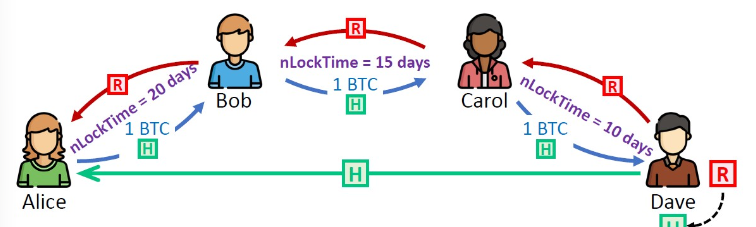
\includegraphics[keepaspectratio]{images/Pasted-image-20260407113700.png}}
Se Alice ha un canale con Bob, e Bob ha un canale con Carol, e Carol ha
un canale con Dave, Alice può instradare il pagamento attraverso Bob e
Carol. I nodi intermedi \textbf{non si fidano l'uno dell'altro} ---
ognuno impegna i propri fondi solo a condizione che il nodo successivo
faccia altrettanto. Questo si ottiene tramite gli \textbf{HTLC}.

\subsection{HTLC: Hashed Timelock
Contract}\label{htlc-hashed-timelock-contract}

L'HTLC è il cuore tecnico del routing sicuro. Combina due meccanismi già
visti --- hash lock e time lock --- in un unico contratto che rende i
pagamenti multi-hop \textbf{atomici}: o tutti i nodi vengono pagati, o
nessuno.

\begin{calloutdefinition}{HTLC (Hashed Timelock Contract)}

Un contratto che condiziona il pagamento alla rivelazione di un
\textbf{segreto preimage} \(R\) tale che \(H(R) = H\) (hash lock), con
un limite di tempo entro il quale il segreto deve essere rivelato (time
lock). Se il segreto non viene rivelato in tempo, i fondi tornano al
mittente.

\end{calloutdefinition}

Il protocollo di pagamento multi-hop funziona così:

\begin{enumerate}
\def\labelenumi{\arabic{enumi}.}
\tightlist
\item
  \textbf{Dave} (destinatario) genera un numero casuale segreto \(R\) e
  calcola il suo hash \(H = H(R)\). Invia \(H\) ad Alice fuori banda
  (es. nell'invoice di pagamento).
\item
  \textbf{Alice} crea un HTLC verso Bob: ``ti pago 1 BTC se riesci a
  darmi l'\(R\) tale che \(H(R) = H\), entro 20 giorni.''
\item
  \textbf{Bob}, sapendo che deve ottenere \(R\) da Dave tramite Carol,
  crea un HTLC verso Carol: ``ti pago 1 BTC se mi dai \(R\), entro 15
  giorni.''
\item
  \textbf{Carol} crea un HTLC verso Dave: ``ti pago 1 BTC se mi dai
  \(R\), entro 10 giorni.''
\item
  \textbf{Dave} rivela \(R\) a Carol e incassa il suo BTC.
\item
  Il segreto \(R\) si propaga all'indietro: Carol lo presenta a Bob, Bob
  lo presenta ad Alice, tutti vengono pagati in cascata.
\end{enumerate}

I timelock sono \textbf{decrescenti} lungo il percorso (20→15→10
giorni): questo garantisce che ogni nodo abbia abbastanza tempo per
riscuotere il proprio pagamento prima del timeout del nodo precedente.
Se Dave non rivela \(R\) entro il termine, tutti i pagamenti vengono
automaticamente rimborsati.

\begin{callouttip}{Atomicità degli HTLC}

Poiché ogni nodo può riscuotere solo presentando \(R\), e \(R\) diventa
noto solo quando Dave lo rivela, l'intera catena di pagamenti è atomica:
o Dave rivela il segreto e tutti vengono pagati, oppure nessuno lo
rivela e i fondi tornano indietro. Un nodo intermedio non può rubare i
fondi.

\end{callouttip}

\subsection{Capacità del Canale e
Liquidità}\label{capacituxe0-del-canale-e-liquidituxe0}

Il routing introduce due concetti fondamentali che spesso vengono
confusi:

\begin{calloutdefinition}{Channel Capacity vs Channel Balance}

La \textbf{channel capacity} è la somma totale dei fondi depositati nel
canale alla sua apertura. È fissa per tutta la vita del canale. Il
\textbf{channel balance} è come quei fondi sono distribuiti tra i due
nodi in un dato momento. Varia dinamicamente ad ogni transazione.

\end{calloutdefinition}

Un nodo che vuole fare routing deve avere \textbf{liquidità in uscita}
(outbound liquidity) verso il nodo successivo. Il routing calcola
percorsi basandosi sulla channel capacity (pubblica), ma non conosce il
channel balance (privato). Questo genera fallimenti di routing: un
canale con capacity 3 BTC potrebbe avere tutto il balance dalla parte
sbagliata, rendendo impossibile instradare 2 BTC in quella direzione. La
conseguenza pratica è che l'algoritmo attuale usa \textbf{brute force
path probing}: prova un percorso, se fallisce ne prova un altro, e così
via --- il che porta a latenze elevate per circa il 5\% dei pagamenti
(oltre 3 minuti).

\subsection{Onion Routing per la
Privacy}\label{onion-routing-per-la-privacy}

Per garantire la privacy, il routing usa una tecnica ispirata a
{[}{[}Tor{]}{]} denominata \textbf{onion routing}: il mittente
costruisce un ``cipolla'' a strati crittografati. Ogni nodo intermedio
può decriptare solo il proprio strato, scoprendo esclusivamente
l'identità del nodo precedente e del successivo --- mai l'intera
traiettoria del pagamento. Questo impedisce ai nodi intermedi di sapere
chi sta pagando chi.

\subsection{Rebalancing dei Canali}\label{rebalancing-dei-canali}

Con l'uso, un canale tende a sbilanciarsi: se Alice paga sempre Bob, il
balance si sposta tutto dal lato di Bob, esaurendo la liquidità in
uscita di Alice. Per ribilanciare, un nodo può eseguire un
\textbf{circular payment} --- instrada un pagamento a se stesso
attraverso un percorso che ripristina i balance desiderati senza costi
di apertura/chiusura di nuovi canali.

\begin{center}\rule{0.5\linewidth}{0.5pt}\end{center}

\section{Stato Attuale e Problemi
Aperti}\label{stato-attuale-e-problemi-aperti}

La Lightning Network ha rilasciato la versione alpha a gennaio 2017. Il
primo acquisto noto tramite Lightning è avvenuto a gennaio 2018. Il 20
marzo 2018 è stato sferrato il primo attacco DDoS, portando offline 200
nodi. Da allora la rete è cresciuta significativamente, con migliaia di
nodi e canali attivi.

Esistono diverse implementazioni open source indipendenti e
interoperabili: C-Lightning, Eclair (Scala), LND (Go), Ptarmigan (C++),
Rust-Lightning, LIT (Python), Electrum. Le specifiche sono pubblicate
come \textbf{BOLT} (Basis Of Lightning Technology), da BOLT \#1
(protocollo base) a BOLT \#11 (protocollo invoice per pagamenti
Lightning).

Per Ethereum esiste la \textbf{Raiden Network/uRaiden}, lanciata sulla
mainnet a novembre 2017, ma non ha avuto lo stesso successo, soppiantata
da altre soluzioni Layer-2 come i rollup.

\subsection{Limiti della Lightning
Network}\label{limiti-della-lightning-network}

La Lightning Network risolve brillantemente il problema della
scalabilità, ma introduce nuovi trade-off:

\textbf{Fund locking}: i fondi depositati nei canali sono immobilizzati
per tutta la durata del canale. Un nodo che vuole fare routing deve
impegnare capitali significativi. Comportamenti disonesti della
controparte possono bloccare i fondi per settimane.

\textbf{Always-on requirement}: senza watchtower, un nodo deve
monitorare la blockchain regolarmente per proteggersi da chiusure
fraudolente. Questo è problematico per i wallet mobile.

\textbf{Centralizzazione strisciante}: ci sono indizi che la rete stia
sviluppando una topologia hub-and-spoke, con pochi nodi hub molto
connessi che gestiscono la maggior parte del routing. Se confermato,
ridurrebbe la decentralizzazione effettiva.

\textbf{Routing inefficiente}: il brute force probing è lento e produce
molti fallimenti. I nuovi algoritmi proposti (gossip-based, ant
algorithms) non sono ancora maturi.

\textbf{Apertura del canale costosa}: si ha bisogno di almeno una
transazione on-chain per aprire ogni canale, il che non è economico
durante periodi di fee elevate.

Resta aperta la domanda centrale posta alla fine della lezione: i canali
off-chain sono una soluzione al trilemma? La risposta è: \emph{non è
ancora dimostrato formalmente}. Migliorano enormemente la scalabilità
senza sacrificare la sicurezza, ma la questione della decentralizzazione
--- specialmente nella topologia del grafo che si sta formando ---
rimane un punto di ricerca attivo.

\newpage

\chapter{(Lab) Bitcoin: Anonimato e
Deanonimizzazione}\label{lab-bitcoin-anonimato-e-deanonimizzazione}

Questa quinta lezione di laboratorio affronta due temi correlati: il
completamento della pipeline di parsing del \texttt{blk.dat} con la
gestione degli UTXO, e l'analisi dell'anonimato in Bitcoin, che è una
delle proprietà più fraintese della blockchain. Il filo conduttore è che
la blockchain è pubblica e persistente: tutto ciò che avviene su di essa
è osservabile, e l'unica protezione offerta nativamente è la
\textbf{pseudonimia}, non l'anonimato vero.

\begin{center}\rule{0.5\linewidth}{0.5pt}\end{center}

\section{Completamento della pipeline: dal blk.dat al CSV con
UTXO}\label{completamento-della-pipeline-dal-blk.dat-al-csv-con-utxo}

\subsection{Il problema degli UTXO nel formato
custom}\label{il-problema-degli-utxo-nel-formato-custom}

Nelle lezioni precedenti si era costruito un formato CSV custom per
rappresentare le transazioni Bitcoin estratte dal \texttt{blk.dat}. Il
formato aveva due problemi principali: i blocchi non erano ordinati per
altezza, e le transazioni non contenevano informazioni dirette sugli
UTXO (cioè, gli input referenziavano le transazioni precedenti per hash,
non per valore). Il metodo \texttt{cleanExactNoUtxo} in Java risolve il
primo problema in modo sequenziale: prima inferisce una mappa da block
hash a block height (\texttt{inferBlockHeightMap}), poi sostituisce gli
hash dei blocchi con le altezze numeriche (\texttt{replaceBlockHashes}),
quindi ordina le transazioni per altezza del blocco
(\texttt{sortPreservingTxOrder}), e infine sostituisce gli hash delle
transazioni e degli indirizzi con ID numerici incrementali a partire da
zero. Il risultato è un file ordinato con ID compatti, adatto a
successive elaborazioni.

Il metodo \texttt{fillItUtxo} affronta invece il secondo problema:
leggendo il CSV ordinato, mantiene in memoria una mappa
\texttt{TreeMap\textless{}TxOutputIds,\ TxOutputCouple\textgreater{}}
che tiene traccia degli output non ancora spesi. Per ogni input di ogni
transazione, consulta questa struttura per recuperare il valore e
l'indirizzo sorgente, aggiungendoli al record dell'input nel CSV. Quando
un UTXO viene consumato, viene rimosso dalla mappa. Il codice gestisce
anche casi limite come le transazioni coinbase (che non hanno input
reali), le incoerenze nel dataset e i fee negativi.

\begin{calloutwarning}{Complessità e ordinamento}

Il metodo \texttt{fillItUtxo} funziona correttamente \textbf{solo} su un
file già ordinato per block height. Senza ordinamento, gli UTXO
verrebbero cercati prima di essere creati, causando errori di lookup
sistematici. La separazione tra \texttt{cleanExactNoUtxo} e
\texttt{fillItUtxo} riflette proprio questa dipendenza sequenziale.

\end{calloutwarning}

\begin{center}\rule{0.5\linewidth}{0.5pt}\end{center}

\section{Anonimato in Bitcoin: pseudonimia e i suoi
limiti}\label{anonimato-in-bitcoin-pseudonimia-e-i-suoi-limiti}

\subsection{Che cosa garantisce
Bitcoin}\label{che-cosa-garantisce-bitcoin}

Bitcoin non è anonimo: è \textbf{pseudonimo}. La differenza è
sostanziale. In un sistema anonimo, le transazioni non sono
riconducibili ad alcun attore. In Bitcoin, ogni transazione è firmata
con la chiave privata dell'indirizzo mittente, e l'intera storia delle
transazioni è pubblica e permanente nella blockchain. L'identità reale
di chi controlla un indirizzo non è direttamente visibile, ma le sue
azioni (movimenti di fondi, tempi, importi) sono completamente
tracciate.

Un utente può generare un numero arbitrario di indirizzi diversi --- è
anzi pratica consigliata usarne uno nuovo per ogni transazione. Ma
questo non rompe la pseudonimia: significa solo che la stessa persona
reale controlla più pseudonimi. Il problema è che le euristiche di
clustering, descritte più avanti, riescono spesso a raggruppare questi
indirizzi ricondizionandoli allo stesso utente.

Un ulteriore punto di debolezza è che le transazioni vengono diffuse
nella rete P2P principalmente dai loro creatori tramite \textbf{gossip}.
Chi le crea le ha firmate, quindi conosce le chiavi private degli input:
è il proprietario degli indirizzi. Questa osservazione è alla base degli
attacchi di network listening.

\begin{center}\rule{0.5\linewidth}{0.5pt}\end{center}

\section{Attacchi di
deanonimizzazione}\label{attacchi-di-deanonimizzazione}

\subsection{La pipeline concettuale}\label{la-pipeline-concettuale}

Un attacco di deanonimizzazione mira a collegare le identità reali del
mondo fisico con gli indirizzi pseudonimi della blockchain. Il processo
si articola in tre stadi progressivi, ciascuno con risorse e strumenti
diversi:

\pandocbounded{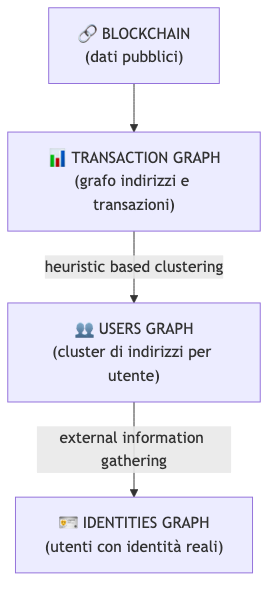
\includegraphics[keepaspectratio,alt={Diagramma Mermaid}]{images/mermaid-lezione-17-lab-bitcoin-anonimato-e-deanonimizzazione-01.png}}
\emph{Fig. --- Pipeline di deanonimizzazione: dalla blockchain al grafo
delle identità reali.}

Il primo stadio è puramente passivo: si costruisce il
\textbf{transaction graph} dalla blockchain pubblica, dove i nodi sono
indirizzi e gli archi rappresentano flussi di fondi. Il secondo stadio
applica \textbf{euristiche di clustering} per raggruppare indirizzi che
probabilmente appartengono allo stesso utente, ottenendo un
\textbf{users graph} dove i nodi sono cluster. Il terzo stadio
arricchisce il users graph con \textbf{informazioni esterne} per
etichettare i cluster con identità reali, producendo
l'\textbf{identities graph}.

\subsection{Clustering euristico}\label{clustering-euristico}

Le euristiche si basano sull'osservazione del comportamento reale degli
utenti Bitcoin e sui vincoli tecnici del protocollo. Sono dipendenti dal
tempo (le abitudini degli utenti cambiano) e non universali: generano
falsi positivi e falsi negativi. La prassi è preferire la riduzione dei
falsi positivi a scapito di un aumento dei falsi negativi, perché
attribuire erroneamente indirizzi a un utente sbagliato è più grave che
non attribuirli affatto.

\begin{calloutdefinition}{Common Inputs Heuristic (euristica degli input comuni)}

Tutti gli indirizzi usati come input in una stessa transazione
appartengono allo stesso utente. La logica è che per firmare gli input
di una transazione servono le chiavi private corrispondenti: solo chi le
possiede tutte può costruire quella transazione. Quindi gli indirizzi di
input condividono necessariamente lo stesso proprietario.

\end{calloutdefinition}

Graficamente, una transazione con input multipli
\texttt{addr\_1,\ addr\_2,\ ...,\ addr\_n} produce un arco tra tutti gli
indirizzi nel users graph, che vengono riuniti nello stesso cluster.
L'implementazione efficiente si riduce a trovare le \textbf{componenti
connesse} del grafo degli input, ottenibile con una BFS in complessità
lineare.

\begin{calloutdefinition}{Change Address Heuristic (euristica dell’indirizzo di resto)}

Quando si spende un UTXO, il valore in eccesso rispetto all'importo
inviato viene restituito al mittente su un nuovo indirizzo, detto
\emph{change address} (indirizzo di resto). L'euristica assume che tale
indirizzo appartenga allo stesso utente degli indirizzi di input.

\end{calloutdefinition}

Identificare il change address non è banale: in una transazione con più
output, quale è il destinatario e quale è il resto? La versione
raffinata dell'euristica definisce criteri precisi:

\begin{callouttip}{Criteri per identificare un change address (versione raffinata)}

L'indirizzo \(c\) è un change address nella transazione \(t\) se e solo
se: - \(t\) non è una transazione coinbase - \(|\text{outputs}(t)| > 1\)
(almeno due output: uno di destinazione, uno di resto) -
\(\text{inputs}(t) \cap \text{outputs}(t) = \emptyset\) (nessun
``self-change'' diretto) - Nessun altro indirizzo negli output di \(t\)
è già noto come change address o appartiene al cluster del mittente - È
la \textbf{prima volta} che \(c\) compare nella blockchain - Nessun
altro indirizzo negli output soddisfa contemporaneamente queste
condizioni (univocità)

\end{callouttip}

La condizione di prima comparsa è particolarmente rilevante: un utente
attento genera un indirizzo fresco per ogni resto, quindi un indirizzo
mai visto prima è un forte indizio che si tratti di un change address.
Regole aggiuntive possono essere introdotte per tenere conto di pattern
comportamentali noti (es. wallet specifici che generano output in un
certo ordine).

\subsection{Raccolta di informazioni
esterne}\label{raccolta-di-informazioni-esterne}

Anche le euristiche più raffinate lavorano solo su dati on-chain. Per
associare cluster a identità reali si ricorre a fonti esterne:

\begin{itemize}
\tightlist
\item
  \textbf{Timing analysis}: se due transazioni avvengono in rapida
  successione, possono essere collegate allo stesso utente o
  dispositivo.
\item
  \textbf{Amount analysis}: importi molto precisi o ricorrenti possono
  rivelare pattern di utilizzo.
\item
  \textbf{Log interni di servizi terzi}: exchange, wallet custodial e
  marketplace raccolgono dati KYC (\emph{Know Your Customer}) e
  indirizzi di consegna fisici. Se le autorità accedono a questi log,
  l'associazione indirizzo--identità è diretta.
\item
  \textbf{Dust attack}: l'attaccante invia una quantità minuscola di BTC
  (\emph{dust}) a un indirizzo bersaglio. Se il wallet della vittima usa
  automaticamente quel UTXO come input in una transazione futura,
  quell'indirizzo viene collegato tramite la common inputs heuristic ad
  altri indirizzi dello stesso utente.
\end{itemize}

Un caso emblematico di informazione esterna è il tweet di WikiLeaks del
14 giugno 2011 che pubblicava esplicitamente il proprio indirizzo di
donazione Bitcoin (\texttt{1HB5XMLmzFVj8ALj6mfBsbifRoD4miY36v}). Da quel
momento in poi, quell'indirizzo è permanentemente e pubblicamente
etichettato nella blockchain.

\subsection{Network listening}\label{network-listening}

Il network listening è una tecnica che mira a correlare un indirizzo
Bitcoin con l'indirizzo IP del suo proprietario, sfruttando le proprietà
del protocollo di diffusione delle transazioni.

Le assunzioni di base (non necessariamente sempre vere) sono due: il
primo nodo a diffondere una nuova transazione nella rete è con alta
probabilità il suo creatore, e il creatore, avendo firmato la
transazione, conosce le chiavi private degli input e quindi è il
proprietario degli indirizzi corrispondenti.

L'attaccante inserisce nella rete P2P un gran numero di \textbf{nodi
ascoltatori} sotto il proprio controllo, con connettività elevata e
connessioni veloci. Grazie all'alta connettività, questi nodi ricevono
le transazioni appena diffuse quasi in contemporanea con i vicini del
creatore. Triangolando i tempi di ricezione tra tutti i nodi
ascoltatori, si stima quale nodo della rete ha originato la transazione.
L'IP del nodo originante viene quindi associato all'indirizzo Bitcoin
degli input.

\begin{calloutwarning}{Limiti del network listening}

L'IP di un nodo non equivale sempre all'identità del proprietario: NAT,
VPN, Tor e proxy possono nasconderlo. Per questo l'attaccante può
raffinare la stima combinando IP con l'insieme degli \emph{entry node}
usati dalla vittima. Inoltre, solo i \textbf{full node} sono
direttamente targetizzabili, poiché i light client non propagano le
transazioni direttamente.

\end{calloutwarning}

\subsection{Topology discovery}\label{topology-discovery}

Il network listening è spesso accoppiato con la \textbf{scoperta della
topologia} della rete P2P. Conoscere la topologia aumenta la precisione
della triangolazione, perché permette di modellare accuratamente il
percorso di propagazione del gossip. Poiché Bitcoin non ha un overlay
strutturato, l'unico modo per conoscere la topologia è chiedere
direttamente ai nodi la loro lista di vicini. Questo processo può
\textbf{corrompere le liste di connessione} degli altri nodi (pollution
attack) e può causare effetti simili a un DoS sulla rete, poiché
richiede connessioni dirette con ogni nodo target.

\begin{center}\rule{0.5\linewidth}{0.5pt}\end{center}

\section{Dataset: Users Graph 2013 e caso
Wikileaks}\label{dataset-users-graph-2013-e-caso-wikileaks}

Come caso di studio pratico, il laboratorio utilizza un sottoinsieme
della blockchain del 2013 relativo a WikiLeaks: i blocchi dalla height
130863 alla 131006 (144 blocchi), contenenti 6094 transazioni che
coinvolgono 8129 indirizzi. L'indirizzo di donazione di WikiLeaks
(\texttt{1HB5XMLmzFVj8ALj6mfBsbifRoD4miY36v}) è l'anchor noto nel
dataset. Il Users Graph 2013 dell'intera blockchain di quell'anno, una
volta costruito e labelizzato, mostra cluster identificabili con servizi
noti come Mt. Gox, Silk Road, BTC-e, Bitstamp e altri exchange o
marketplace, evidenziando come la deanonimizzazione pratica fosse già
possibile a quell'epoca.

\begin{calloutnote}{Assignment del laboratorio}

Costruire il \textbf{users graph} come mappa indirizzo → cluster ID
applicando la \textbf{common inputs heuristic} al dataset Wikileaks
sopra descritto. Il tip suggerito è di ridurre il problema al calcolo
delle \textbf{componenti connesse} del grafo degli input, risolvibile
con una BFS in complessità lineare \(O(V + E)\).

\end{calloutnote}

\begin{center}\rule{0.5\linewidth}{0.5pt}\end{center}

\section{Tracciamento dei furti: taint
analysis}\label{tracciamento-dei-furti-taint-analysis}

La natura pubblica e immutabile della blockchain può essere usata anche
in senso difensivo. Quando un furto di Bitcoin viene reso pubblico,
l'indirizzo del ladro diventa noto a tutta la community. Gli utenti
onesti possono tracciare i movimenti dei fondi rubati e applicare
\textbf{blacklisting} sugli indirizzi del ladro. In pratica, è difficile
tracciare con certezza \emph{tutti} i fondi rubati, ma è spesso
sufficiente tracciarne una piccola parte fino a un servizio terzo (un
exchange, un mixer) per stabilire con alta probabilità che il ladro ne
detiene il controllo.

\begin{calloutdefinition}{Taint Analysis (analisi della contaminazione)}

Il \textbf{taint value} dell'indirizzo \(A\) rispetto all'indirizzo
\(B\) è la percentuale dei fondi attualmente in possesso di \(A\) che
possono essere fatti risalire a \(B\). Formalmente misura la dipendenza
economica tra due indirizzi lungo la catena delle transazioni.

\end{calloutdefinition}

La taint analysis è uno strumento di base per seguire fondi rubati ma
non tiene conto della \emph{proprietà}: sa che i fondi sono passati per
un certo indirizzo, ma non chi lo controlla. Due casi storici illustrano
l'applicazione:

\begin{itemize}
\tightlist
\item
  \textbf{Furto allinvain} (13/06/2011, 25.001 BTC): l'analisi del
  transaction graph mostrò i fondi convergere verso il servizio
  MyBitcoin attraverso una serie di transazioni intermedie,
  identificando percorsi di movimento con timestamp precisi.
\item
  \textbf{Ransomware TorrentLocker 2 (CryptoWall 2)} (15/09/2014,
  target: PA italiana): il malware richiedeva riscatti in Bitcoin.
  Tracciando gli indirizzi delle vittime note fu possibile seguire parte
  dei fondi raccolti e identificare gli exchange usati per il cashout.
\end{itemize}

\begin{center}\rule{0.5\linewidth}{0.5pt}\end{center}

\section{Contromisure per la privacy}\label{contromisure-per-la-privacy}

\subsection{CoinJoin e CoinShuffle}\label{coinjoin-e-coinshuffle}

\textbf{CoinJoin} (2013) è la prima contromisura collaborativa: più
utenti si accordano per unire i propri input in un'unica transazione
grande, firmata collettivamente. L'accordo può avvenire tramite un
server di rendezvous centralizzato o tramite consensus decentralizzato.
Si possono costruire catene di transazioni CoinJoin per aumentare
l'offuscamento. I limiti principali sono che l'anonimato all'interno di
ogni transazione è limitato al numero di partecipanti, che esiste
linkabilità interna (gli output sono ancora osservabili), che è
vulnerabile a DoS da parte di partecipanti malevoli, e che nascondere
gli IP dei partecipanti richiede strumenti aggiuntivi.

\textbf{CoinShuffle} (2014) migliora CoinJoin introducendo un protocollo
di shuffling crittografico degli output che elimina la linkabilità
interna: nemmeno il server di coordinamento può sapere quale output
corrisponde a quale input.

\subsection{Tecniche di offuscamento}\label{tecniche-di-offuscamento}

Indipendentemente da CoinJoin, esistono tecniche individuali per
spezzare il tracciamento della proprietà:

{\def\LTcaptype{none} % do not increment counter
\begin{longtable}[]{@{}
  >{\raggedright\arraybackslash}p{(\linewidth - 2\tabcolsep) * \real{0.5000}}
  >{\raggedright\arraybackslash}p{(\linewidth - 2\tabcolsep) * \real{0.5000}}@{}}
\toprule\noalign{}
\begin{minipage}[b]{\linewidth}\raggedright
Tecnica
\end{minipage} & \begin{minipage}[b]{\linewidth}\raggedright
Descrizione
\end{minipage} \\
\midrule\noalign{}
\endhead
\bottomrule\noalign{}
\endlastfoot
\textbf{Split} & Divide un UTXO in molti output piccoli verso indirizzi
diversi \\
\textbf{Aggregation} & Aggrega molti UTXO piccoli in uno grande per
rompere il grafo \\
\textbf{Peeling chain} & Invia una quantità fissa ripetutamente,
mantenendo un ``residuo'' che scorre verso un indirizzo fresco a ogni
passo \\
\textbf{Binary tree} & Struttura ad albero di transazioni per
distribuire i fondi su molteplici rami \\
\end{longtable}
}

La \textbf{peeling chain} è particolarmente visibile nell'analisi
on-chain: genera una sequenza lineare di transazioni dove ogni nodo ha
un output di importo fisso (il pagamento) e uno di importo decrescente
(il residuo). Si riconosce facilmente e non offre vera protezione a un
analista esperto.

\subsection{Mixer}\label{mixer}

I \textbf{mixer} (o tumbler) sono servizi che accettano Bitcoin da un
utente e restituiscono la stessa quantità (meno fee) prelevandola dai
fondi di altri utenti, spezzando così completamente la catena di
proprietà on-chain. Non esiste link diretto tra l'indirizzo di invio e
quello di ricezione.

\begin{calloutwarning}{Problemi dei mixer}

\begin{itemize}
\tightlist
\item
  Sono \textbf{terze parti centralizzate}: richiedono fiducia e
  introducono un single point of failure
\item
  Addebitano \textbf{commissioni}
\item
  Devono proteggere e \textbf{distruggere permanentemente} i log interni
\item
  Per importi grandi il processo è lento e insicuro (rischio di
  deanonimizzazione o furto da parte del mixer stesso)
\item
  Catene di mixer aumentano i costi e la probabilità di furto ad ogni
  hop
\end{itemize}

Alternativa pratica: il \textbf{chain hopping}, ovvero spostare i fondi
su una blockchain diversa (es. Monero) per poi tornare su Bitcoin con un
indirizzo nuovo, sfruttando la migliore privacy nativa di quella chain.

\end{calloutwarning}

\newpage

\chapter{Hard and Soft Forks in
Bitcoin}\label{hard-and-soft-forks-in-bitcoin}

Un \textbf{fork} è, in senso generale, una modifica al protocollo e alle
strutture dati di una rete blockchain. Nel mondo del software
tradizionale si parla semplicemente di aggiornamenti; nel contesto delle
criptovalute questi aggiornamenti assumono un nome e una rilevanza
speciale, perché non avvengono su un sistema centralizzato ma su una
rete distribuita di nodi che devono raggiungere il consenso sulle regole
del gioco. I fork possono essere motivati dall'introduzione di nuove
funzionalità, dalla correzione di vulnerabilità di sicurezza,
dall'affrontare problemi di scalabilità, o dalla necessità di risolvere
disaccordi profondi all'interno della comunità di sviluppatori e miner.

\section{Tipi di Fork}\label{tipi-di-fork}

\subsection{Protocol Fork vs Chain
Fork}\label{protocol-fork-vs-chain-fork}

È fondamentale distinguere due fenomeni che vengono entrambi chiamati
``fork'' ma hanno natura molto diversa.

Un \textbf{protocol fork} (\emph{fork di protocollo}) nasce da un
cambiamento deliberato nelle regole di consenso. È un aggiornamento
intenzionale e coordinato: alcuni nodi adottano le nuove regole, altri
no. Se i nodi seguono regole incompatibili, si crea una divisione
permanente della blockchain in due catene separate, ognuna con la
propria storia futura e i propri asset. I protocol fork si distinguono
in due categorie --- \textbf{soft fork} (compatibile con le versioni
precedenti) e \textbf{hard fork} (non compatibile).

Un \textbf{chain fork} (\emph{fork di catena}) è invece un fenomeno
temporaneo e fisiologico. Accade quando due miner trovano un blocco
valido quasi contemporaneamente, oppure a causa della latenza di rete o
di un attacco. Si creano così più blocchi validi alla stessa altezza. La
rete risolve l'ambiguità applicando la \textbf{longest chain rule} (la
regola della catena con più lavoro cumulativo): uno dei rami diventa
orfano e i suoi blocchi vengono scartati. Non cambia nessuna regola, non
nasce nessun nuovo asset. È un evento normale nell'operatività
quotidiana di Bitcoin.

\pandocbounded{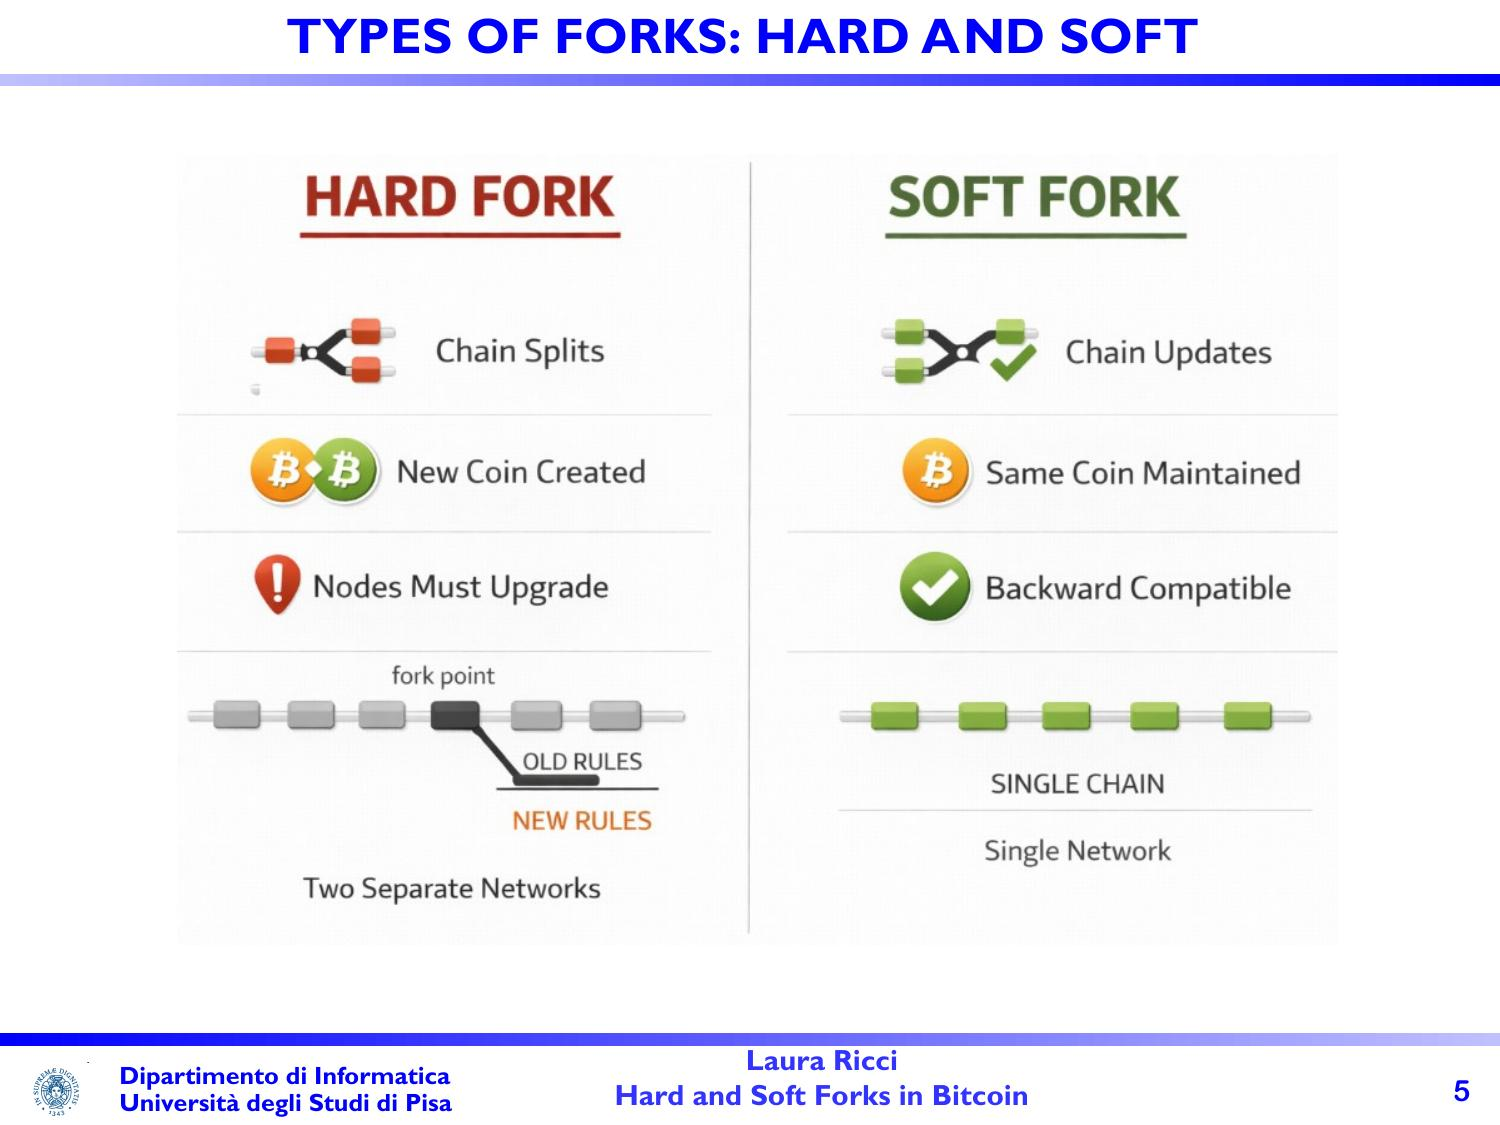
\includegraphics[keepaspectratio,alt={Confronto visivo Hard Fork vs Soft Fork: chain splits, backward compatibility}]{images/lezione-18-hard-and-soft-forks-in-bitcoin-img-01.jpg}}
\emph{Fig. --- Hard fork vs soft fork a confronto: il primo divide la
rete in due catene separate, il secondo mantiene la rete unita con
regole più restrittive.}

\begin{callouttip}{Intuizione chiave}

La distinzione chiave è: il protocol fork cambia le regole, il chain
fork è una gara temporanea tra blocchi validi che si risolve
automaticamente. Solo il primo può generare una divisione permanente
della blockchain.

\end{callouttip}

\begin{center}\rule{0.5\linewidth}{0.5pt}\end{center}

\section{Soft Fork}\label{soft-fork}

\begin{calloutdefinition}{Soft Fork}

Un soft fork è una modifica all'implementazione di una blockchain che è
\textbf{backward compatible} (retrocompatibile): i nodi non aggiornati
possono continuare a interagire con quelli aggiornati. In generale, un
soft fork introduce regole più restrittive rispetto a quelle precedenti.

\end{calloutdefinition}

L'esempio classico è la riduzione della dimensione massima dei blocchi:
un nodo non aggiornato, programmato per accettare blocchi fino a 2 MB,
accetterà senza problemi blocchi da 1 MB prodotti dai nodi aggiornati.
Il vincolo nuovo è un sottoinsieme dei vincoli vecchi.

\subsection{Accettazione del Fork}\label{accettazione-del-fork}

Il meccanismo con cui un soft fork viene adottato è simile a un
\textbf{voto distribuito}. Quando gli sviluppatori propongono un
aggiornamento, stabiliscono una data futura per la sua attivazione. Nel
frattempo, i miner possono segnalare il proprio supporto codificando un
numero di versione aggiornato nei blocchi che minano. Gli altri nodi
della rete osservano quante versioni aggiornate circolano e possono
stimare quanta potenza di hashing ha già adottato il cambiamento.

Il processo funziona così: i miner consapevoli delle nuove regole
segnalano supporto tramite i \textbf{version bits}, ma non le applicano
ancora. Le nuove regole diventano attive solo quando la soglia di
approvazione viene raggiunta. Il famoso BIP66 del 2015 --- che
modificava il formato delle firme digitali --- ottenne il 95\% della
potenza di hashing prima di essere attivato.

\begin{calloutnote}{BIP (Bitcoin Improvement Proposal)}

I BIP sono il meccanismo formale attraverso cui vengono proposte
modifiche al protocollo Bitcoin. Chiunque può aprire un BIP; la sua
adozione dipende dall'accordo della comunità e dei miner.

\end{calloutnote}

\subsection{Come Muore la Vecchia
Versione}\label{come-muore-la-vecchia-versione}

Dopo un soft fork, se la maggioranza della potenza di hashing adotta le
nuove regole, la versione legacy sparisce gradualmente. Il motivo è
puramente economico: i blocchi prodotti dai nodi non aggiornati vengono
rifiutati dalla maggioranza dei nodi aggiornati. I miner non vogliono
sprecare potenza computazionale producendo blocchi che la rete scarterà,
quindi migrano alla nuova versione per continuare a ricevere ricompense.

\pandocbounded{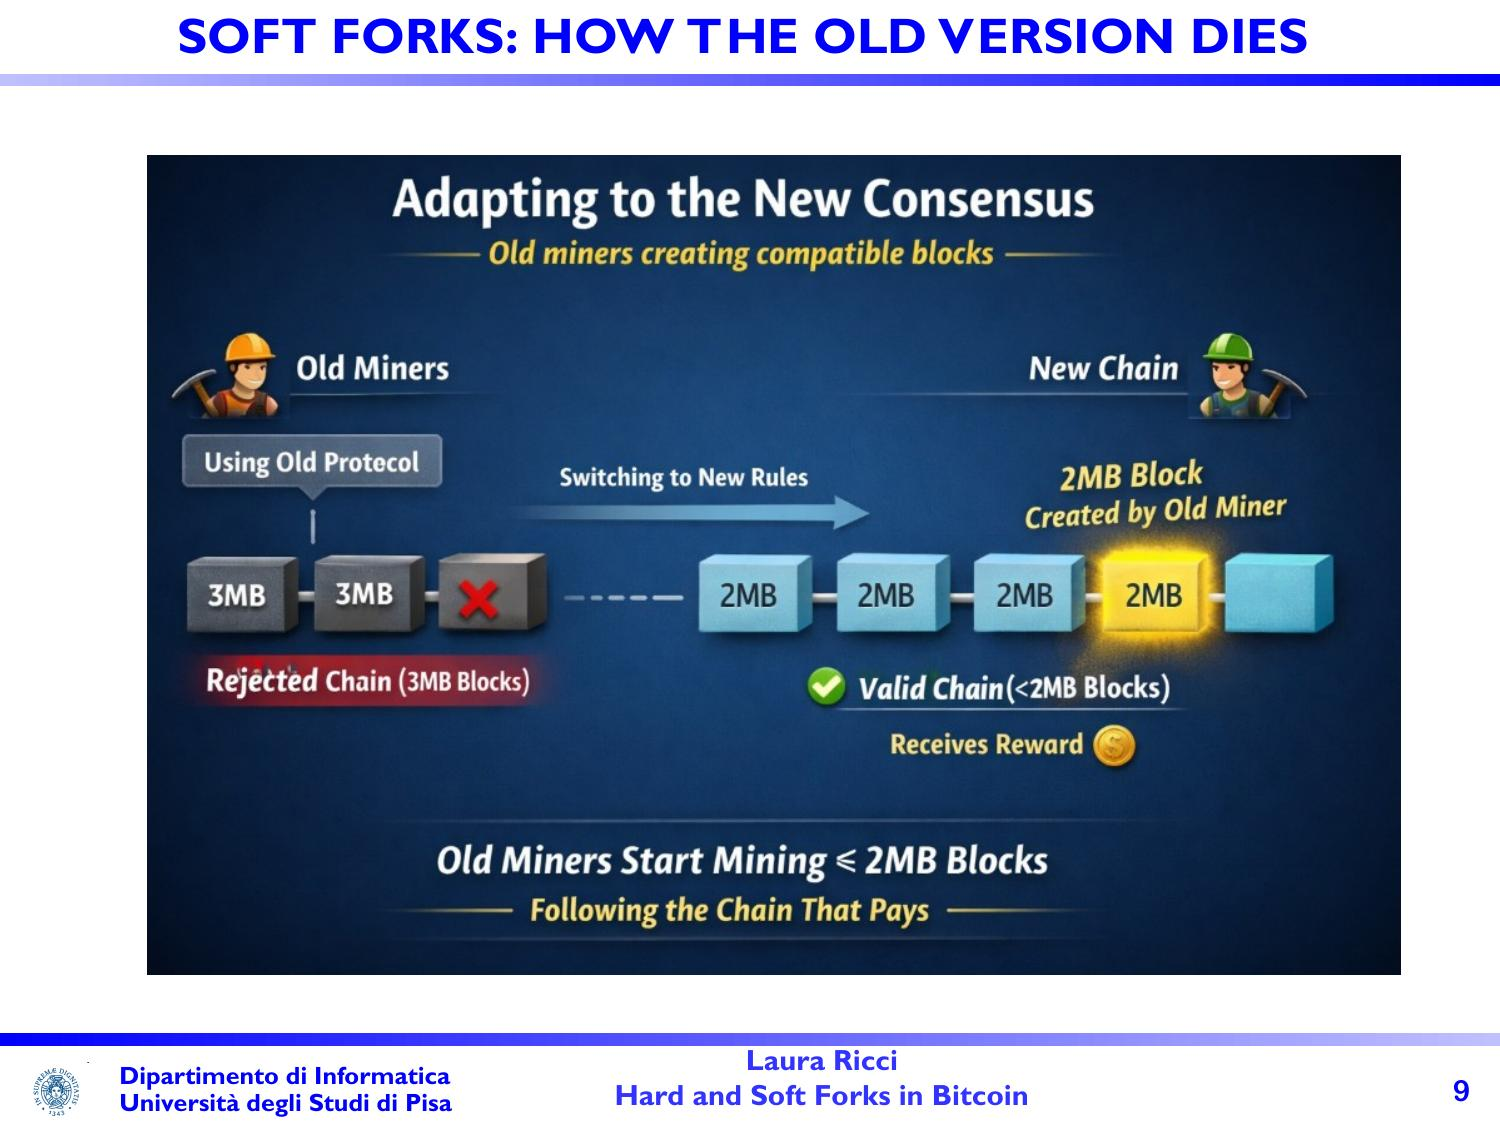
\includegraphics[keepaspectratio,alt={Diagramma ``Adapting to the New Consensus'': i vecchi miner abbandonano la catena rifiutata e migrano a quella valida}]{images/lezione-18-hard-and-soft-forks-in-bitcoin-img-02.jpg}}
\emph{Fig. --- Come la vecchia versione muore: i blocchi dei nodi non
aggiornati vengono rifiutati dalla catena dominante. I miner seguono
``the chain that pays''.}

I possibili esiti di un soft fork sono tre: tutti i miner accettano e il
fork è semplicemente un aggiornamento software; la maggioranza accetta,
la nuova versione si consolida e quella vecchia muore gradualmente; la
maggioranza rifiuta e il fork non sopravvive.

\begin{center}\rule{0.5\linewidth}{0.5pt}\end{center}

\section{I Principali Soft Fork di
Bitcoin}\label{i-principali-soft-fork-di-bitcoin}

Prima di analizzare SegWit e Taproot nel dettaglio, è utile avere una
visione d'insieme dei soft fork che hanno caratterizzato la storia di
Bitcoin.

\pandocbounded{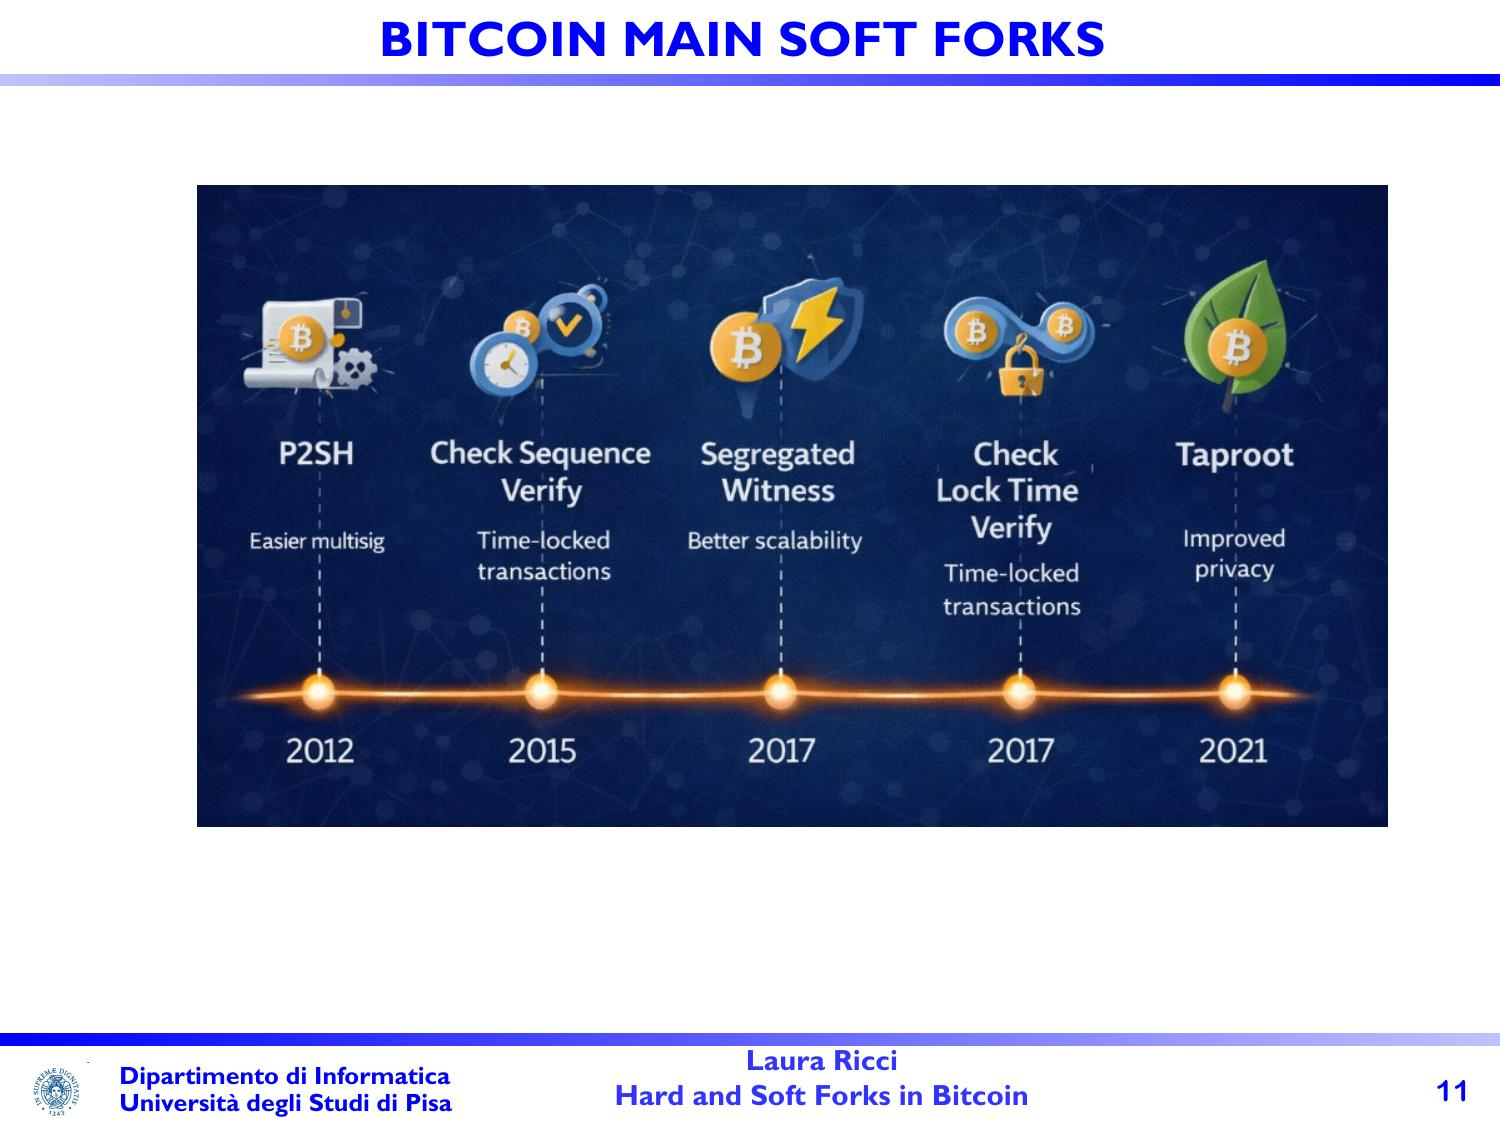
\includegraphics[keepaspectratio,alt={Timeline dei principali soft fork Bitcoin: P2SH (2012), CSV (2015), SegWit (2017), CLTV (2017), Taproot (2021)}]{images/lezione-18-hard-and-soft-forks-in-bitcoin-img-03.jpg}}
\emph{Fig. --- Timeline dei soft fork principali di Bitcoin: da P2SH
(2012) per il multisig, a SegWit (2017) per la scalabilità, fino a
Taproot (2021) per la privacy.}

\begin{center}\rule{0.5\linewidth}{0.5pt}\end{center}

\section{SegWit --- Agosto 2017}\label{segwit-agosto-2017}

\textbf{SegWit} (\emph{Segregated Witness}, testimone segregato) è il
più importante soft fork della storia di Bitcoin, attivato nell'agosto
2017. Per capire cosa ha cambiato, è necessario partire dal problema che
risolveva.

\subsection{Il Problema: Transaction
Malleability}\label{il-problema-transaction-malleability}

Prima di SegWit, una transazione Bitcoin conteneva tre componenti
principali: gli \textbf{input} (da dove provengono i bitcoin), gli
\textbf{output} (dove vanno), e le \textbf{firme} (la prova che il
mittente ha autorizzato la transazione). Le firme erano incluse nei dati
della transazione stessa. Questo creava una vulnerabilità nota come
\textbf{transaction malleability} (\emph{malleabilità delle
transazioni}): un attaccante poteva modificare leggermente i dati della
firma senza invalidare la transazione, ma cambiando così il
\textbf{txid} (l'identificatore della transazione). Il txid cambiato
rendeva impossibile per altri protocolli --- come la Lightning Network
--- fare riferimento in modo affidabile a una transazione non ancora
confermata.

\subsection{La Soluzione: Separare la Firma dai
Dati}\label{la-soluzione-separare-la-firma-dai-dati}

SegWit risolve il problema spostando i dati delle firme fuori dalla
struttura principale della transazione, in una sezione separata chiamata
\textbf{Witness} (\emph{testimone}). Poiché il txid viene ora calcolato
senza i dati della firma, non può più essere alterato dopo che la
transazione è stata firmata.

\pandocbounded{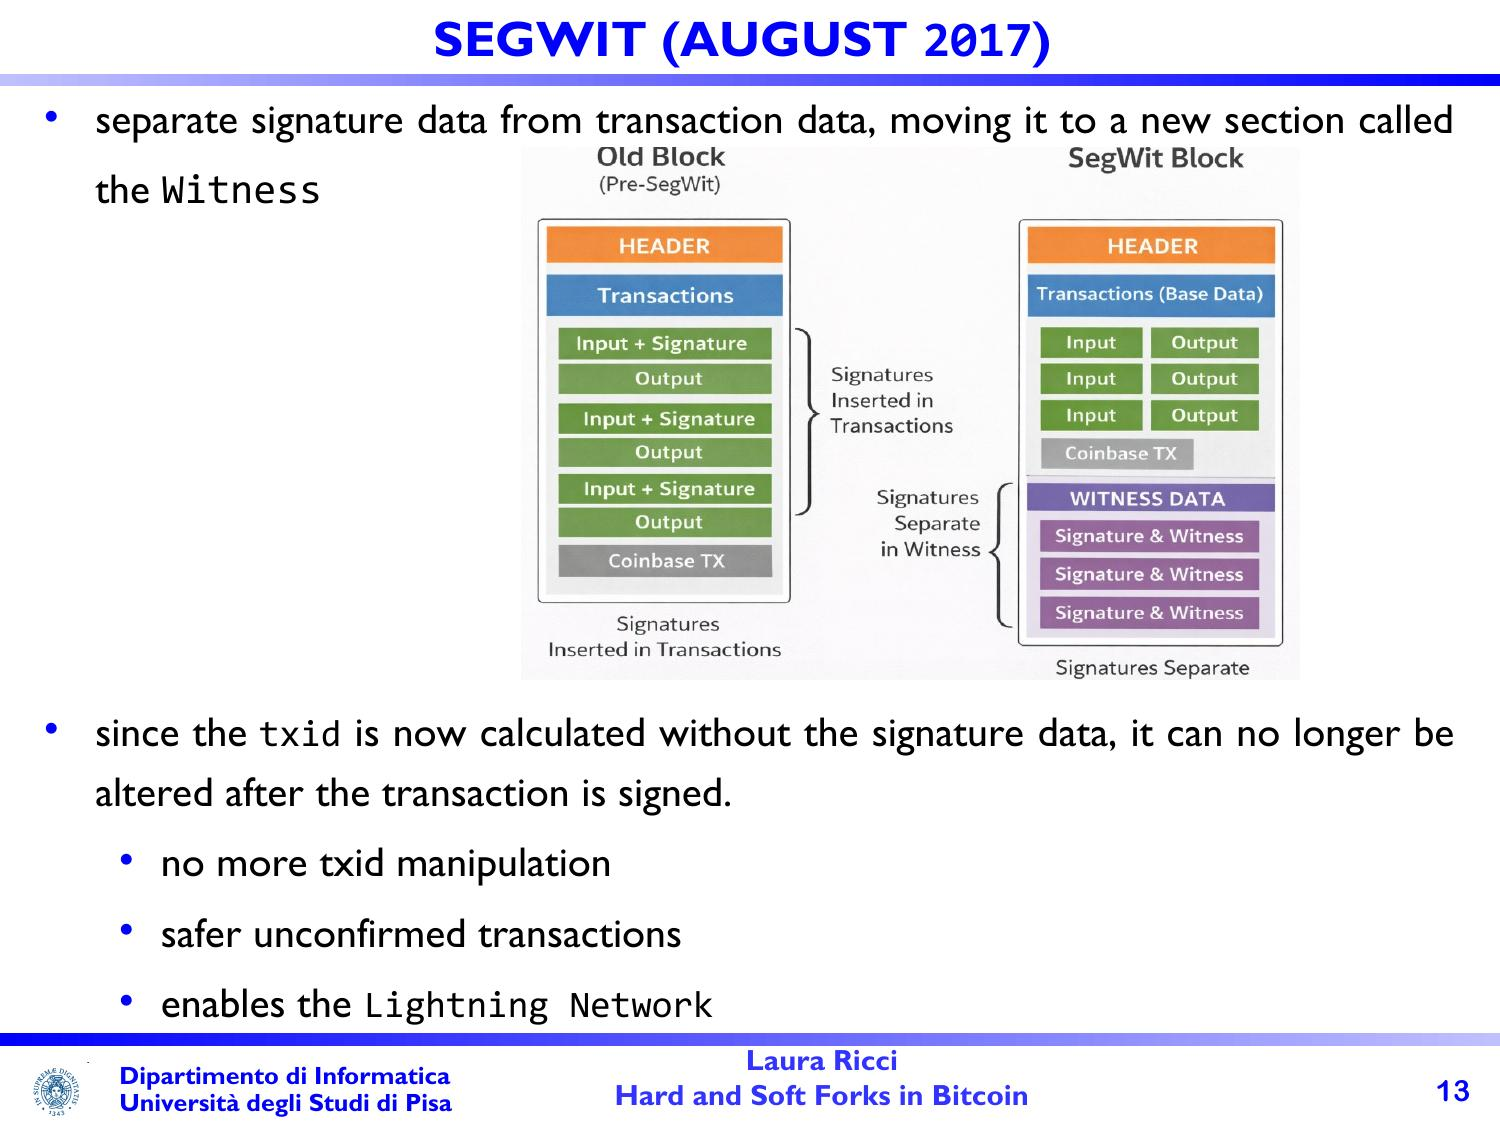
\includegraphics[keepaspectratio,alt={Struttura della transazione pre-SegWit vs post-SegWit: le firme vengono spostate nel Witness separato}]{images/lezione-18-hard-and-soft-forks-in-bitcoin-img-04.jpg}}
\emph{Fig. --- Confronto strutturale: nel blocco Pre-SegWit le firme
sono embedded nella transazione; nel blocco SegWit la Witness Data è
segregata e non influisce sul calcolo del txid.}

I benefici sono: eliminazione della manipolazione del txid, transazioni
non confermate più sicure, e l'abilitazione della Lightning Network.

\begin{calloutwarning}{SegWit è davvero un soft fork?}

Apparentemente SegWit sembrerebbe incompatibile con i nodi vecchi, ma
gli sviluppatori hanno usato un ``trucco'': le firme vengono spostate
fuori dalla parte che i nodi vecchi contano per il calcolo del peso del
blocco. I vecchi nodi non analizzano il Witness, vedono blocchi ≤ 1 MB e
non violano nessuna regola. Accettano i nuovi blocchi senza sapere che
contengono dati Witness.

\end{calloutwarning}

\subsection{Block Weight e Aumento della
Capacità}\label{block-weight-e-aumento-della-capacituxe0}

Anche se non era l'obiettivo primario, SegWit ha aumentato de facto la
capacità di transazione. Prima di SegWit i blocchi erano limitati a 1
MB. SegWit introduce il concetto di \textbf{block weight} (\emph{peso
del blocco}): i byte normali di una transazione contano 4 unità di peso
ciascuno, mentre i byte del Witness contano solo 1 unità di peso. Il
limite massimo è 4 milioni di unità di peso. Questo significa che
blocchi con molte transazioni SegWit possono contenere più dati totali,
pur rimanendo entro il limite di peso --- effettivamente aumentando il
throughput.

\pandocbounded{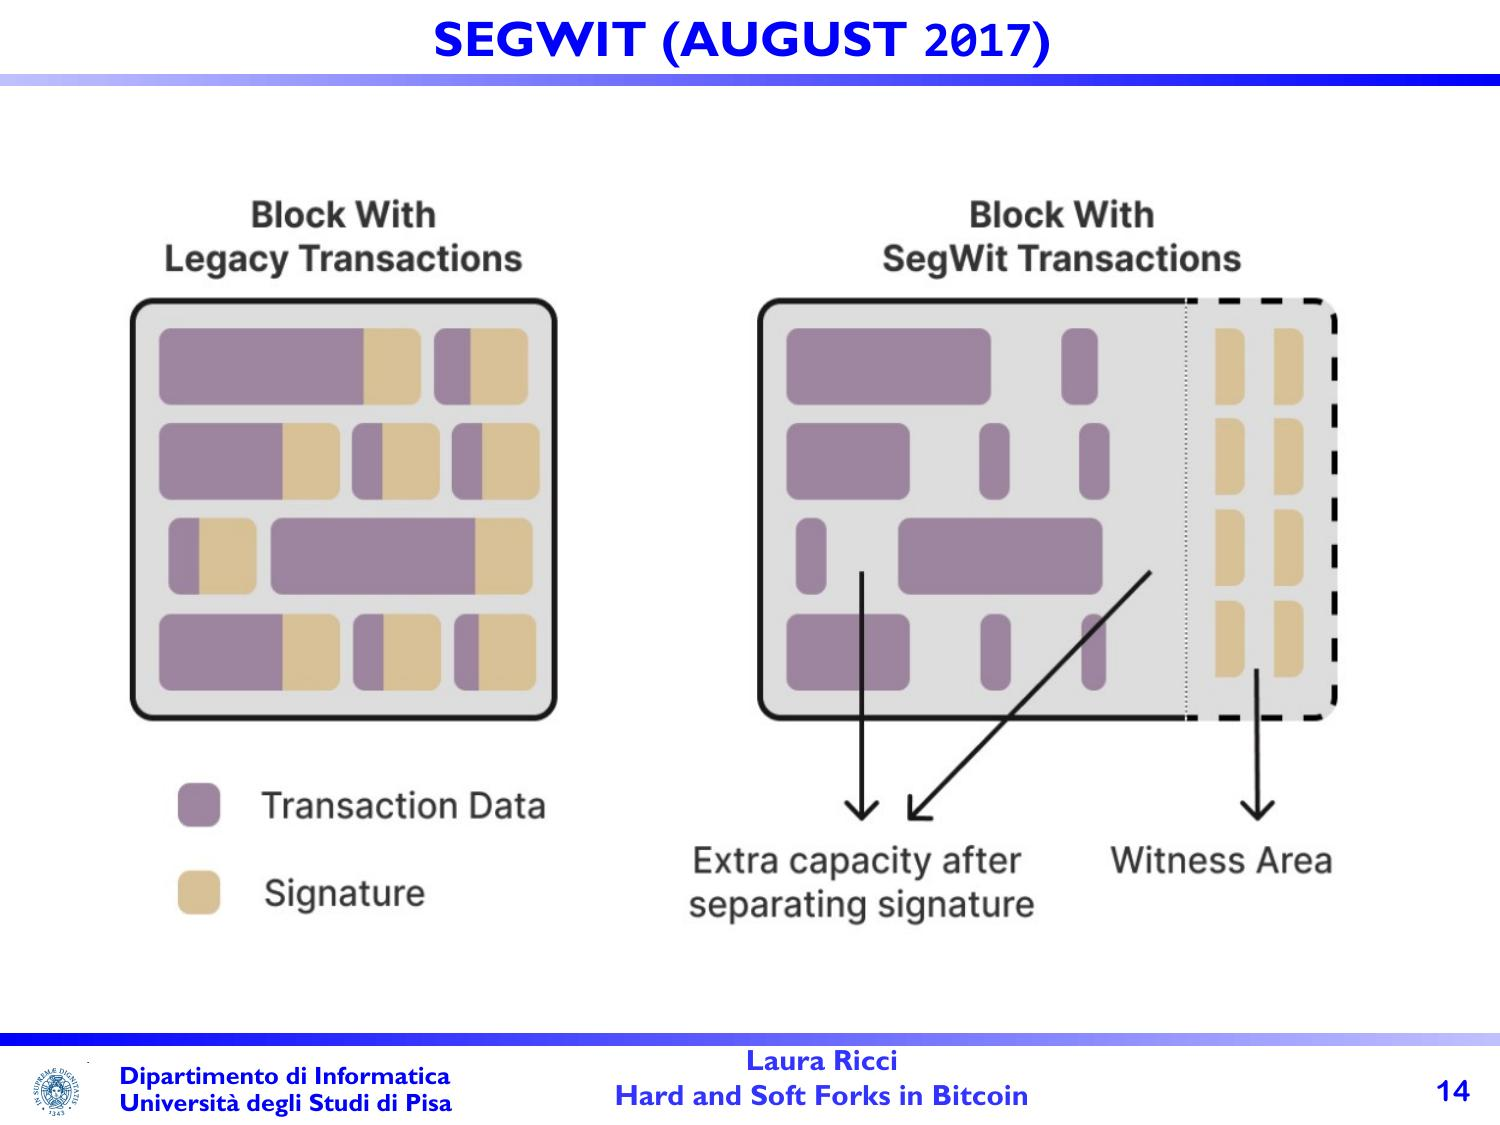
\includegraphics[keepaspectratio,alt={Confronto blocco legacy vs blocco SegWit: la Witness Area permette capacità extra separata dalla base data}]{images/lezione-18-hard-and-soft-forks-in-bitcoin-img-05.jpg}}
\emph{Fig. --- In un blocco SegWit la Witness Area (tratteggiata)
contiene le firme a peso ridotto. La base data rimane ≤ 1 MB per i
vecchi nodi, ma il blocco reale può superarla.}

\subsection{SegWit: Ricapitolazione}\label{segwit-ricapitolazione}

Il diagramma seguente riassume in modo completo il funzionamento di
SegWit, evidenziando come i vecchi nodi vedano solo la parte base del
blocco (≤ 1 MB) e ignorino la witness, mantenendo la retrocompatibilità.

\pandocbounded{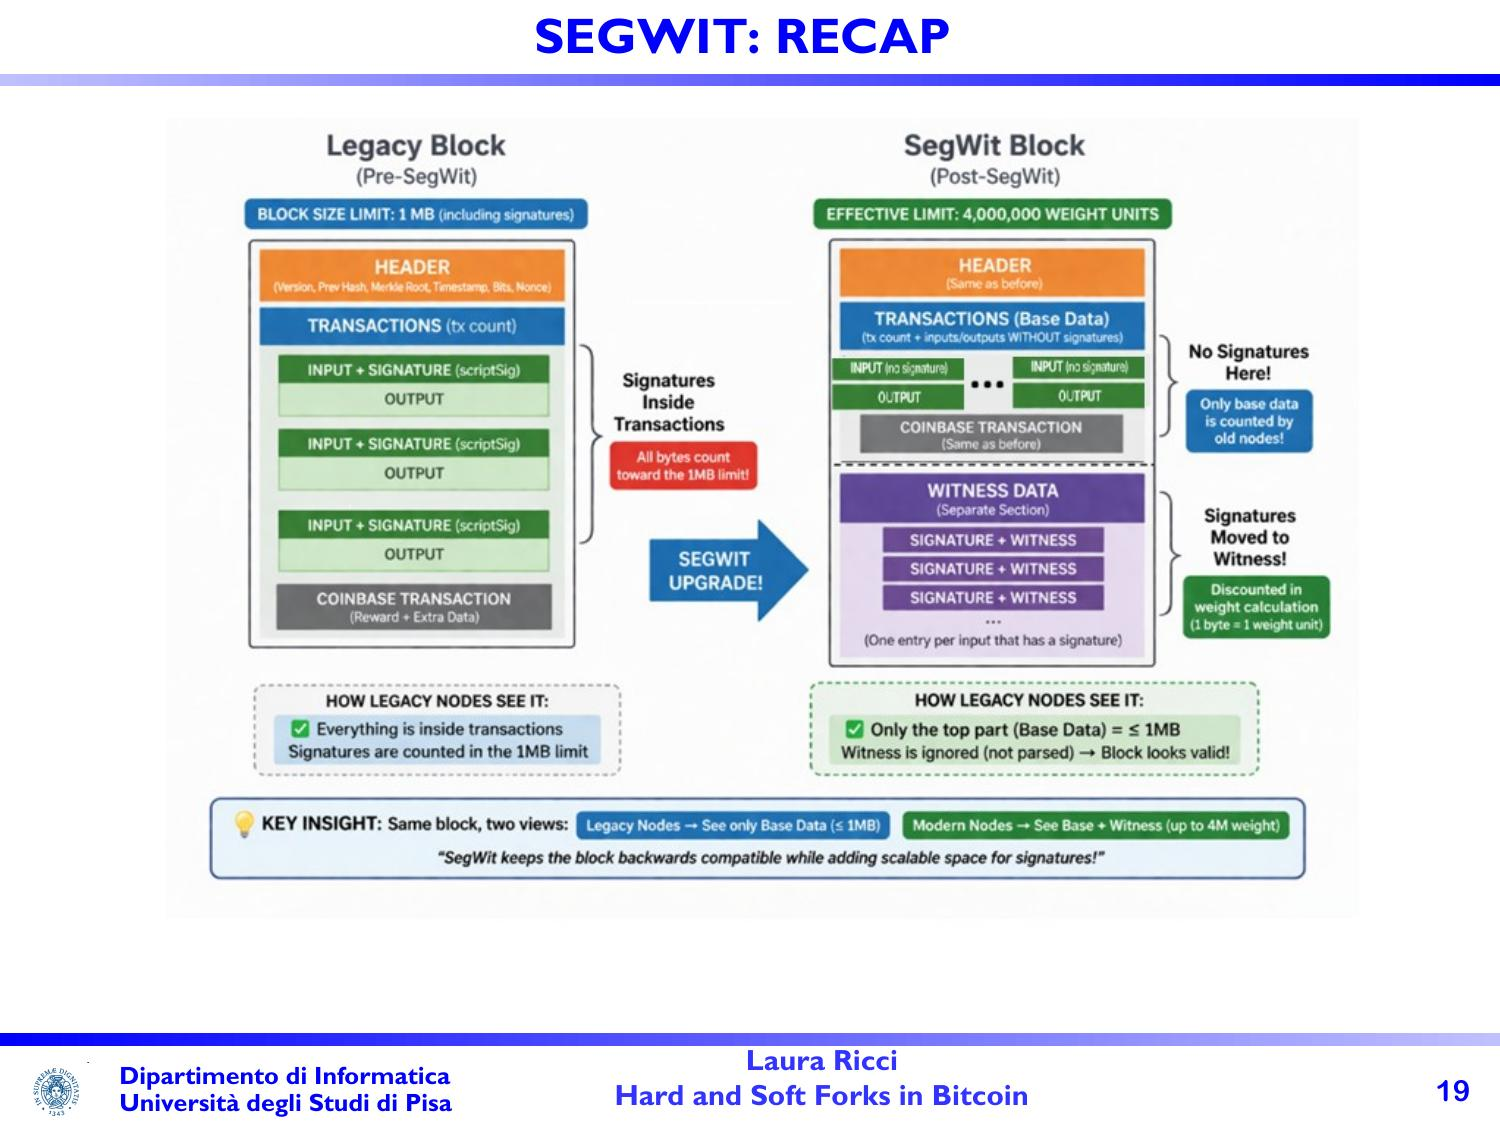
\includegraphics[keepaspectratio,alt={SegWit Recap: confronto Legacy Block vs SegWit Block con indicazione di cosa vedono i vecchi nodi e i nuovi nodi}]{images/lezione-18-hard-and-soft-forks-in-bitcoin-img-06.jpg}}
\emph{Fig. --- Ricapitolazione SegWit: il blocco legacy ha firme inline;
il blocco SegWit le separa nel Witness. I vecchi nodi vedono solo la
base data e rimangono sincronizzati.}

\begin{center}\rule{0.5\linewidth}{0.5pt}\end{center}

\section{Taproot --- Novembre 2021}\label{taproot-novembre-2021}

\textbf{Taproot} è il secondo grande soft fork di Bitcoin, attivato il
14 novembre 2021 con il supporto di oltre il 90\% dei miner. Si basa su
due tecniche crittografiche: le \textbf{Schnorr Signatures} e il
\textbf{MAST} (\emph{Merkelized Abstract Syntax Tree}). L'obiettivo è
migliorare sia le capacità di scripting che la privacy della rete
Bitcoin.

\subsection{Schnorr Signatures}\label{schnorr-signatures}

\begin{calloutdefinition}{Schnorr Signatures (Firme di Schnorr)}

Schema di firma digitale basato sul problema del logaritmo discreto.
Alternativa alle firme ECDSA usate da Bitcoin, con proprietà
crittografiche superiori.

\end{calloutdefinition}

Le Schnorr Signatures hanno cinque proprietà fondamentali:

\textbf{Privacy}: non è possibile distinguere firme individuali in un
gruppo aggregato.

\textbf{Linearità}: consentono un metodo semplice ed efficiente per far
sì che più parti collaboranti producano una firma valida per la somma
delle loro chiavi pubbliche. Questo è il fondamento del \textbf{key
aggregation} (\emph{aggregazione di chiavi}) --- più firmatari possono
produrre una singola firma collettiva indistinguibile da quella di un
singolo firmatario.

\textbf{Batch verification} (\emph{verifica in batch}): con ECDSA,
verificare tre firme richiede tre operazioni separate. Con Schnorr è
possibile verificare tutte e tre insieme in una sola operazione:
\(\text{Ver}(\sigma_1 + \sigma_2 + \sigma_3) = 1\ \text{operazione}\),
contro
\(\text{Ver}(\sigma_1) + \text{Ver}(\sigma_2) + \text{Ver}(\sigma_3) = 3\ \text{operazioni}\)
con ECDSA.

\textbf{Non malleabilità}: le firme non possono essere modificate.

\textbf{Sicurezza dimostrabile}: la sicurezza è riducibile formalmente
al problema del logaritmo discreto.

\pandocbounded{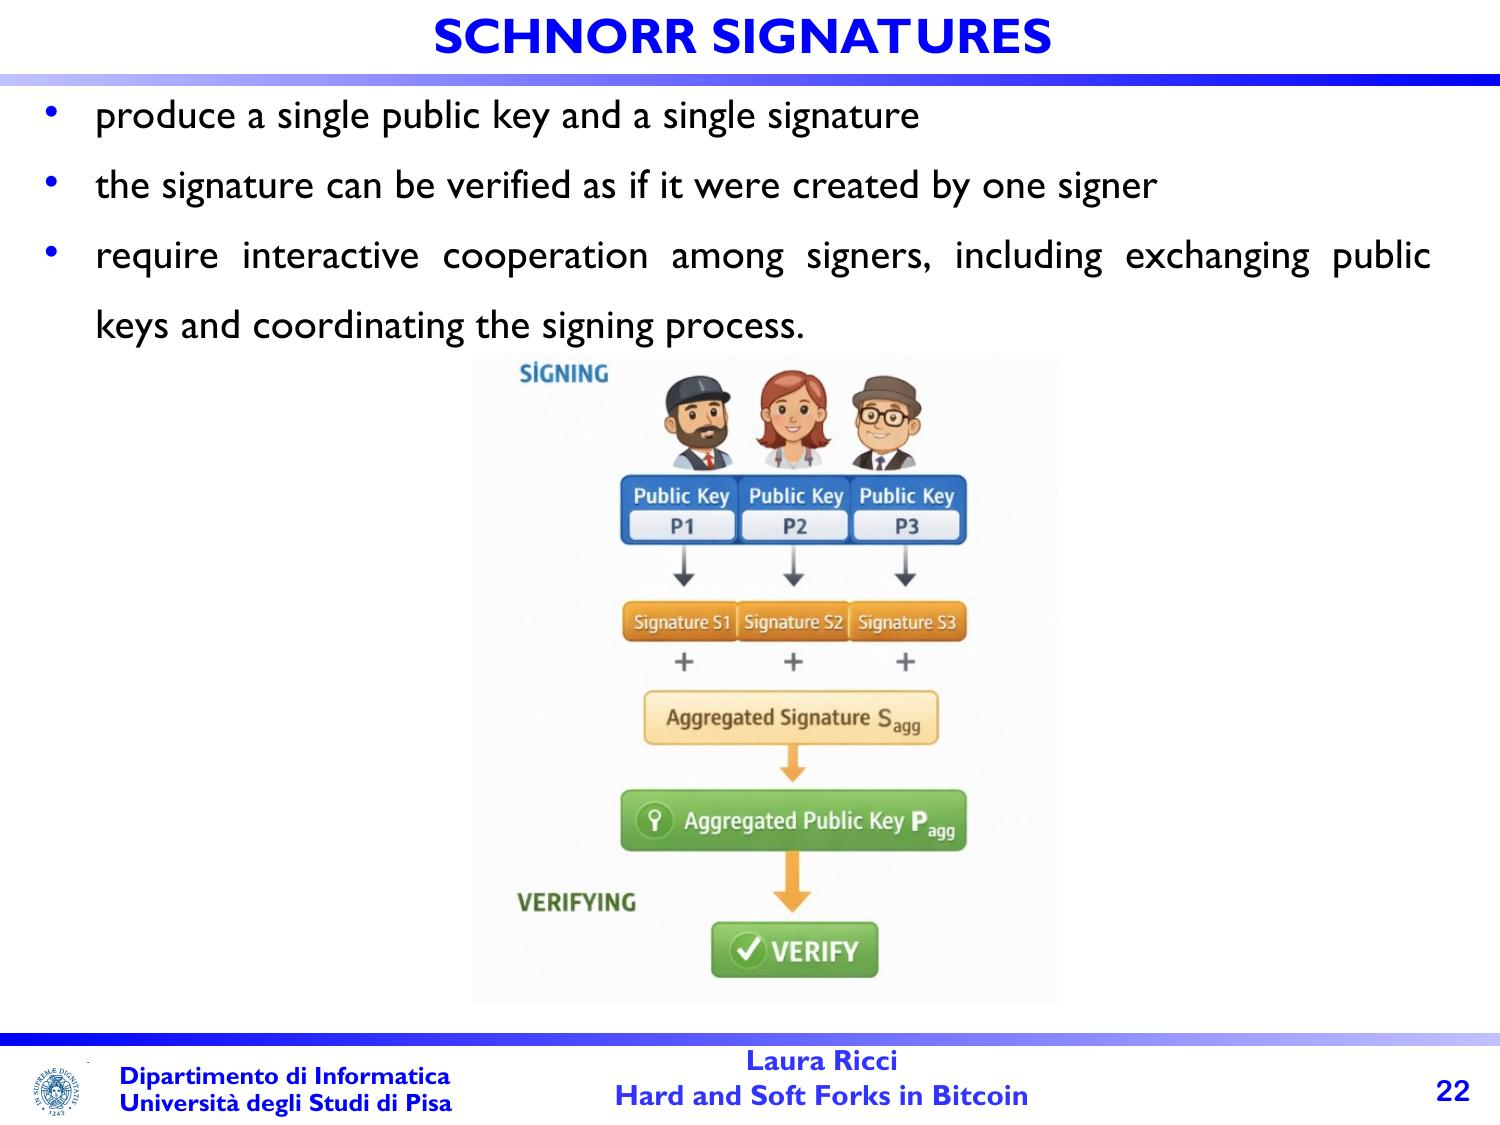
\includegraphics[keepaspectratio,alt={Schema di aggregazione Schnorr: tre firmatari (P1, P2, P3) producono chiave e firma aggregate verificabili come una sola}]{images/lezione-18-hard-and-soft-forks-in-bitcoin-img-07.jpg}}
\emph{Fig. --- Key aggregation con Schnorr: P1, P2, P3 combinano chiavi
e firme in un'unica \(P_{agg}\) e \(S_{agg}\). La verifica è identica a
quella di un firmatario singolo.}

Le Schnorr Signatures producono una singola chiave pubblica e una
singola firma, anche quando più firmatari cooperano. Il processo
richiede cooperazione interattiva tra i firmatari, incluso lo scambio di
chiavi pubbliche e la coordinazione del processo di firma.

\subsection{MAST --- Merkelized Abstract Syntax
Tree}\label{mast-merkelized-abstract-syntax-tree}

\begin{calloutdefinition}{MAST (Merkelized Abstract Syntax Tree)}

Struttura dati che combina un \textbf{Abstract Syntax Tree} (AST) con un
\textbf{Merkle Tree} per rappresentare condizioni di spesa multiple in
modo efficiente e privato.

\end{calloutdefinition}

Il problema che MAST risolve è il seguente: uno script Bitcoin può
prevedere molteplici condizioni di spesa alternative. Senza MAST, tutte
le condizioni devono essere incluse nella transazione quando si spende,
rivelando tutte le clausole anche quelle non usate. MAST permette di
includere nella transazione solo la condizione effettivamente eseguita,
insieme alla Merkle proof che dimostra che quella condizione era nel set
originale.

\subsubsection{La Parte AST}\label{la-parte-ast}

L'\textbf{Abstract Syntax Tree} specifica come suddividere la logica di
spesa in foglie. Le condizioni in relazione OR diventano foglie separate
--- se basta soddisfarne una, non ha senso includerle tutte. Le
condizioni in relazione AND rimangono nella stessa foglia, perché devono
essere soddisfatte insieme.

\pandocbounded{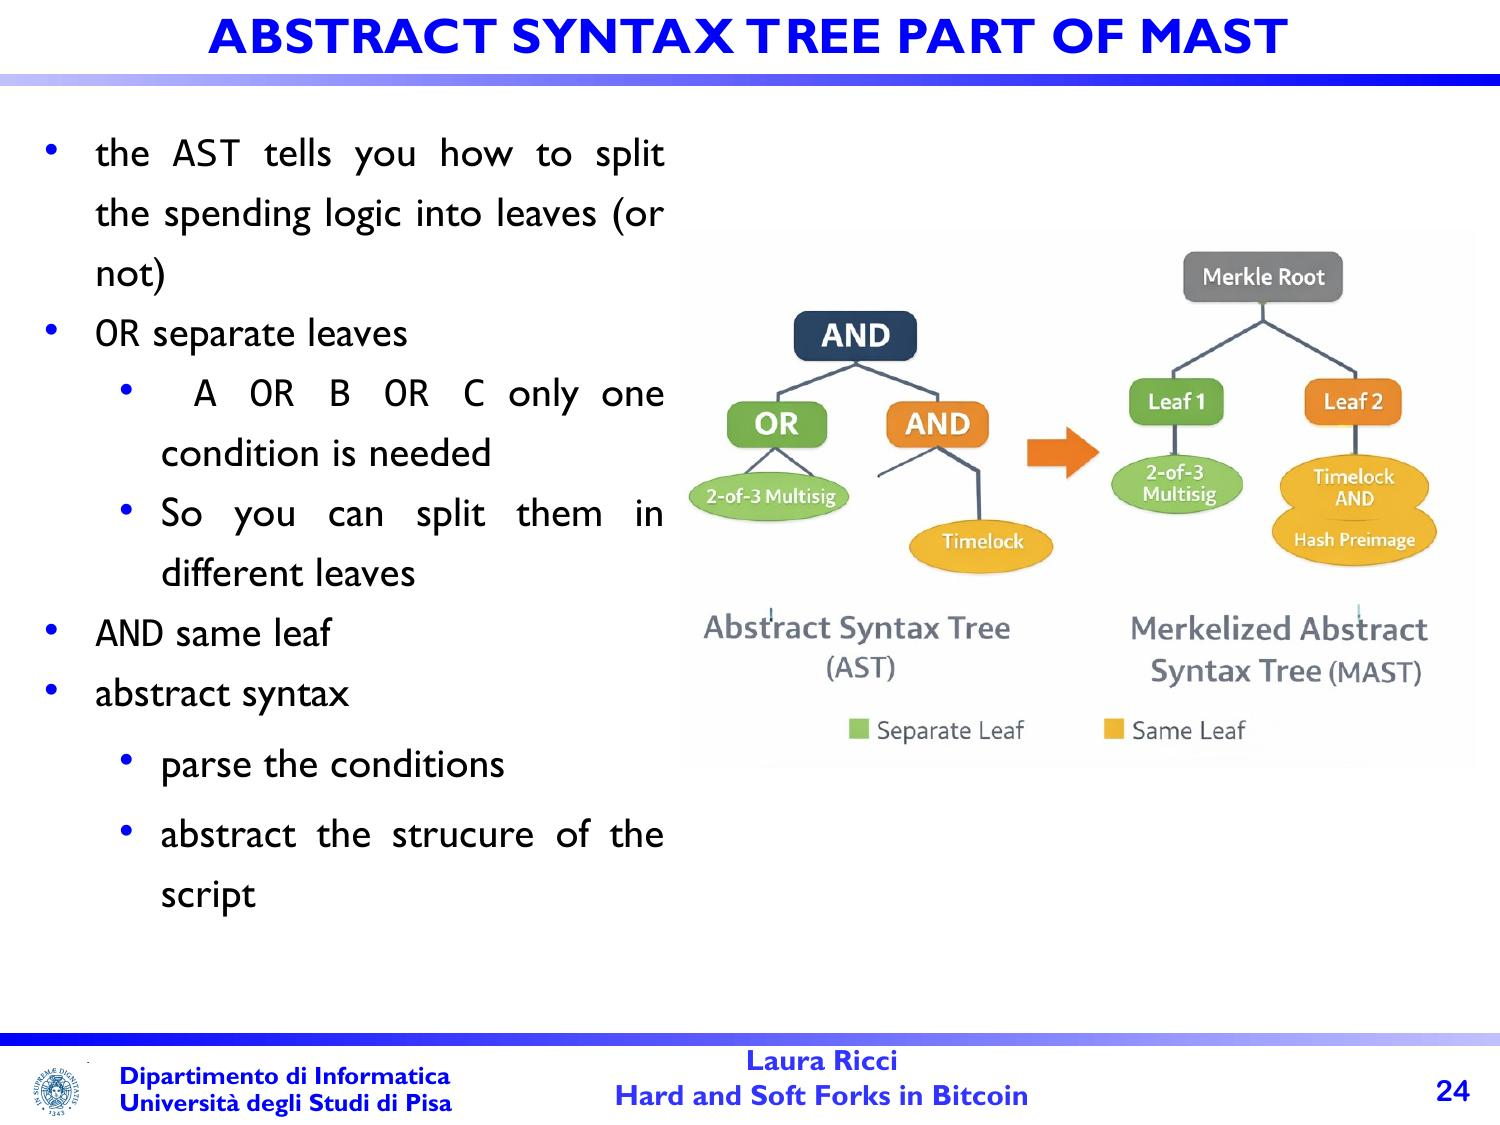
\includegraphics[keepaspectratio,alt={Trasformazione da Abstract Syntax Tree (AST) a Merkelized AST (MAST): le condizioni OR diventano foglie separate, le AND rimangono nella stessa foglia}]{images/lezione-18-hard-and-soft-forks-in-bitcoin-img-08.jpg}}
\emph{Fig. --- Da AST a MAST: le condizioni OR (2-of-3 Multisig,
Timelock) diventano foglie separate; le condizioni AND (Timelock AND
Hash Preimage) rimangono nella stessa foglia.}

\subsubsection{La Parte Merkle Tree}\label{la-parte-merkle-tree}

Una volta strutturate le condizioni come foglie, si costruisce un Merkle
Tree su di esse. La radice del Merkle Tree impegna crittograficamente
tutte le condizioni. Quando si spende, si rivela solo la foglia usata e
il percorso di verifica (Merkle proof), non le altre condizioni.

\pandocbounded{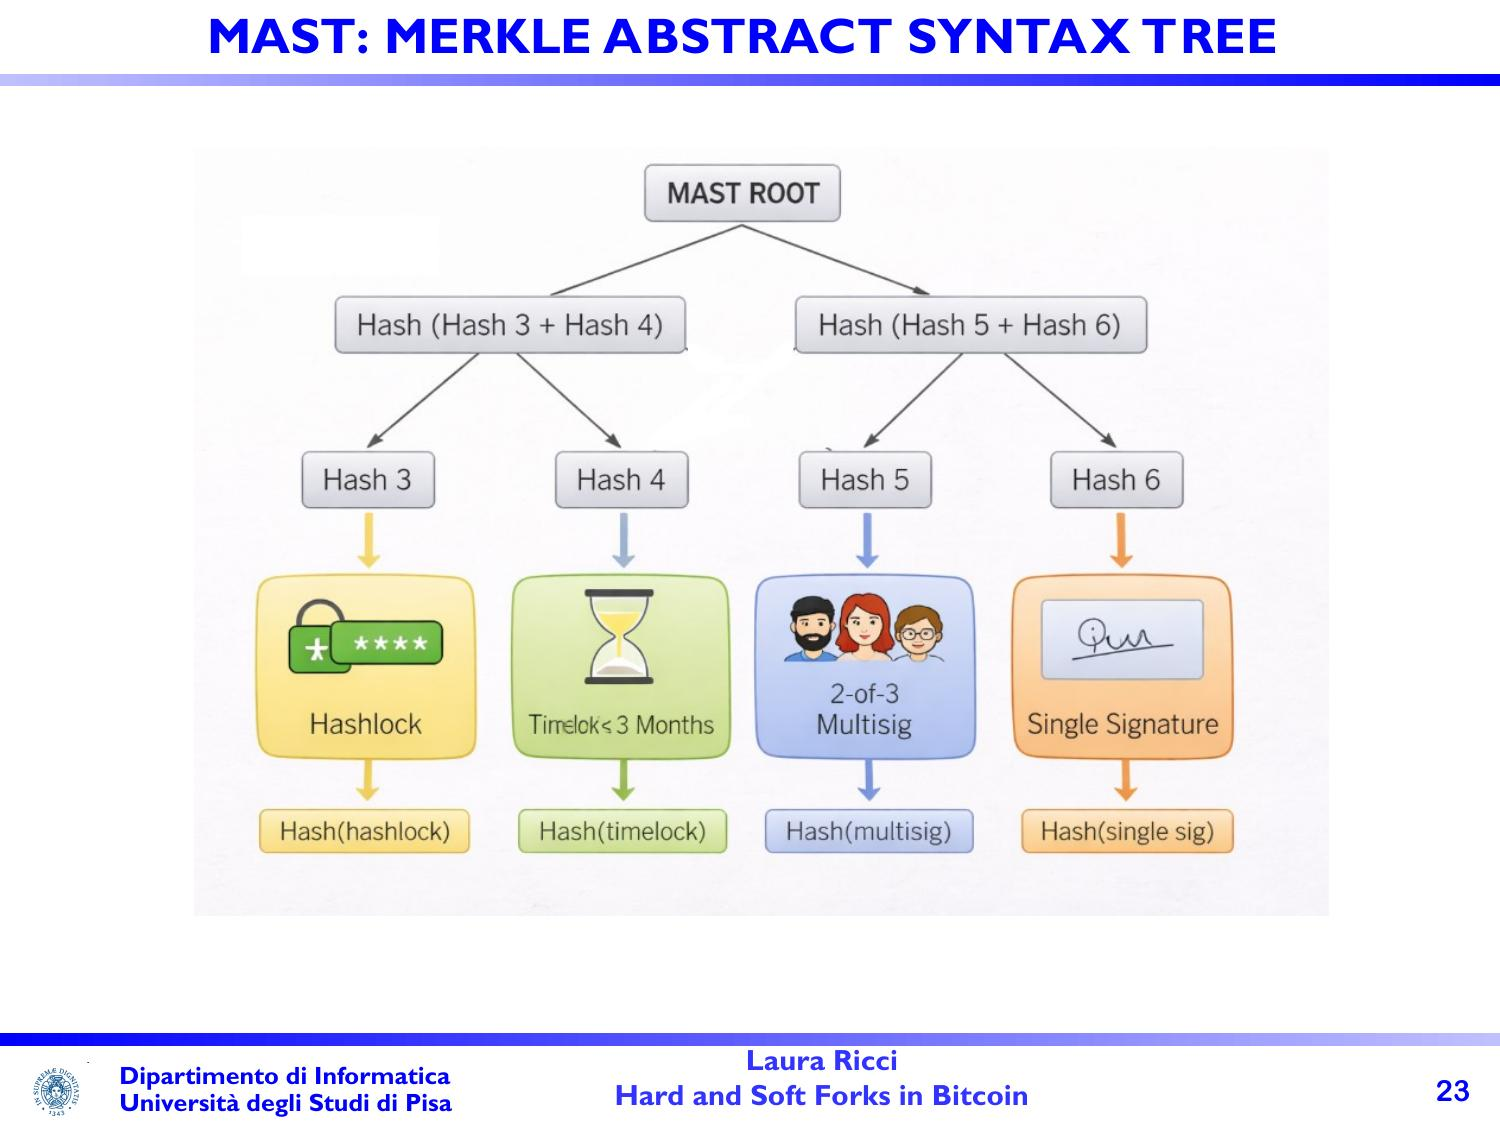
\includegraphics[keepaspectratio,alt={Struttura Merkle Tree del MAST con quattro condizioni di spesa: Hashlock, Timelock ≤3 mesi, 2-of-3 Multisig, Single Signature}]{images/lezione-18-hard-and-soft-forks-in-bitcoin-img-09.jpg}}
\emph{Fig. --- Il Merkle Tree del MAST: ogni condizione di spesa è una
foglia. La MAST ROOT impegna tutte le condizioni. Al momento della spesa
si rivela solo la foglia usata + il Merkle path.}

\begin{callouttip}{MAST con 4 condizioni di spesa}

Supponiamo di avere: - Script 1: multisig 2-di-3 (Alice, Bob, Charlie) -
Script 2: timelock di 1 anno - Script 3: hash preimage - Script 4: firma
singola di Alice

\textbf{Senza MAST}: tutti e 4 gli script sono inclusi nella
transazione, rivelando tutte le clausole.

\textbf{Con MAST}: solo lo script eseguito + la Merkle proof sono
inclusi. Gli altri script rimangono nascosti.

\end{callouttip}

\subsection{La Tweaked Public Key}\label{la-tweaked-public-key}

Il meccanismo con cui Taproot unisce Schnorr Signatures e MAST è la
\textbf{tweaked public key} (\emph{chiave pubblica modificata}). Si
parte da: - una chiave pubblica \(P\) (può essere singola o aggregata da
più firmatari) - la radice del Merkle tree degli script (MAST): \(m\)

Si calcola il \textbf{tweak} come: \[
t = H(P \,\|\, m)
\] dove \(H\) è una funzione hash e \(\|\) indica la concatenazione. Si
applica poi il tweak alla chiave pubblica tramite operazione sulla curva
ellittica: \[
P' = P + t \cdot G
\] Il risultato \(P'\) è la \textbf{tweaked public key}: una nuova
chiave pubblica che impegna crittograficamente sia la chiave interna
\(P\) che l'intero albero di script \(m\).

\pandocbounded{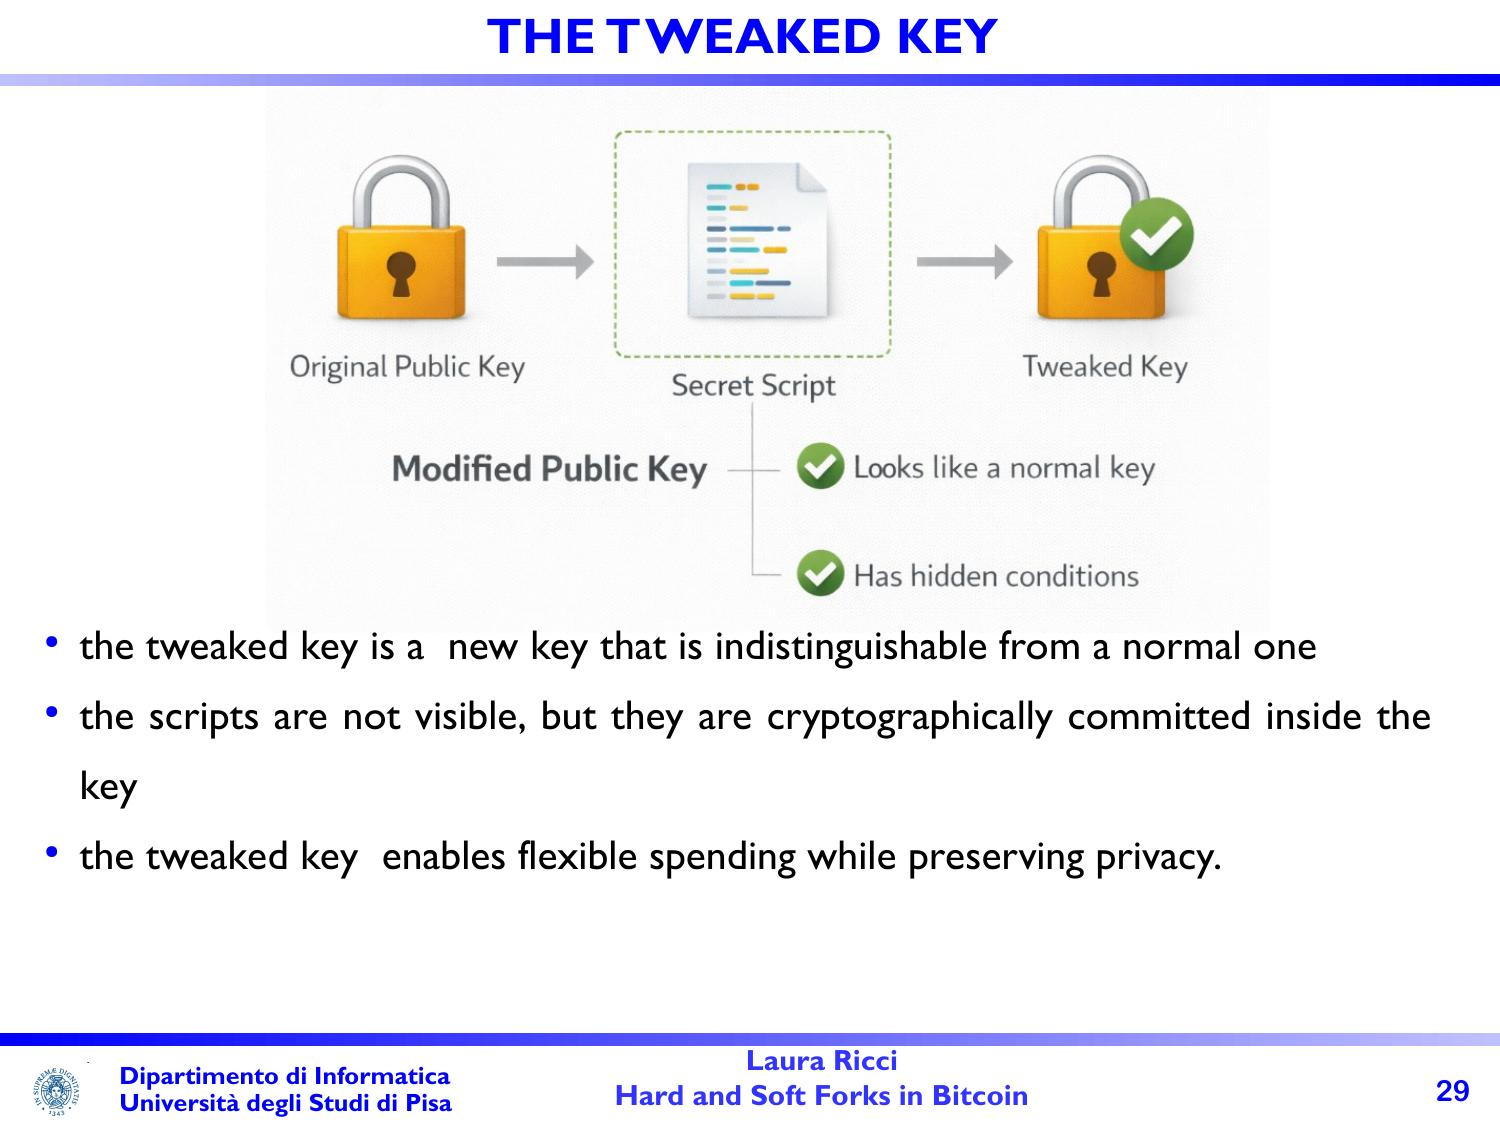
\includegraphics[keepaspectratio,alt={Schema concettuale tweaked key: Original Public Key + Secret Script producono una Tweaked Key che sembra normale ma ha condizioni nascoste}]{images/lezione-18-hard-and-soft-forks-in-bitcoin-img-10.jpg}}
\emph{Fig. --- La tweaked key: combina la chiave pubblica originale con
lo script segreto (MAST root) in un'unica chiave che appare normale
on-chain ma impegna crittograficamente le condizioni di spesa.}

\begin{callouttip}{Cosa viene scritto on-chain}

Sull'output della blockchain non viene scritta né la chiave pubblica
separatamente né la radice MAST separatamente. Viene scritto solo il
singolo valore \(P'\) --- la tweaked key. Questo valore è
indistinguibile da una normale chiave pubblica Schnorr. Gli script sono
invisibili, ma sono crittograficamente impegnati all'interno della
chiave.

\end{callouttip}

\subsection{Key Path vs Script Path
Spending}\label{key-path-vs-script-path-spending}

Taproot prevede due modalità di spesa:

\textbf{Key path spending} (\emph{spesa via chiave}): se tutte le parti
coinvolte sono d'accordo, producono una firma Schnorr aggregata valida
per \(P'\). Nessuno script viene rivelato. Dall'esterno sembra una
semplice transazione a firma singola, anche se in realtà ci sono
molteplici condizioni possibili. Questo è il caso ``felice'' e più
privato.

\pandocbounded{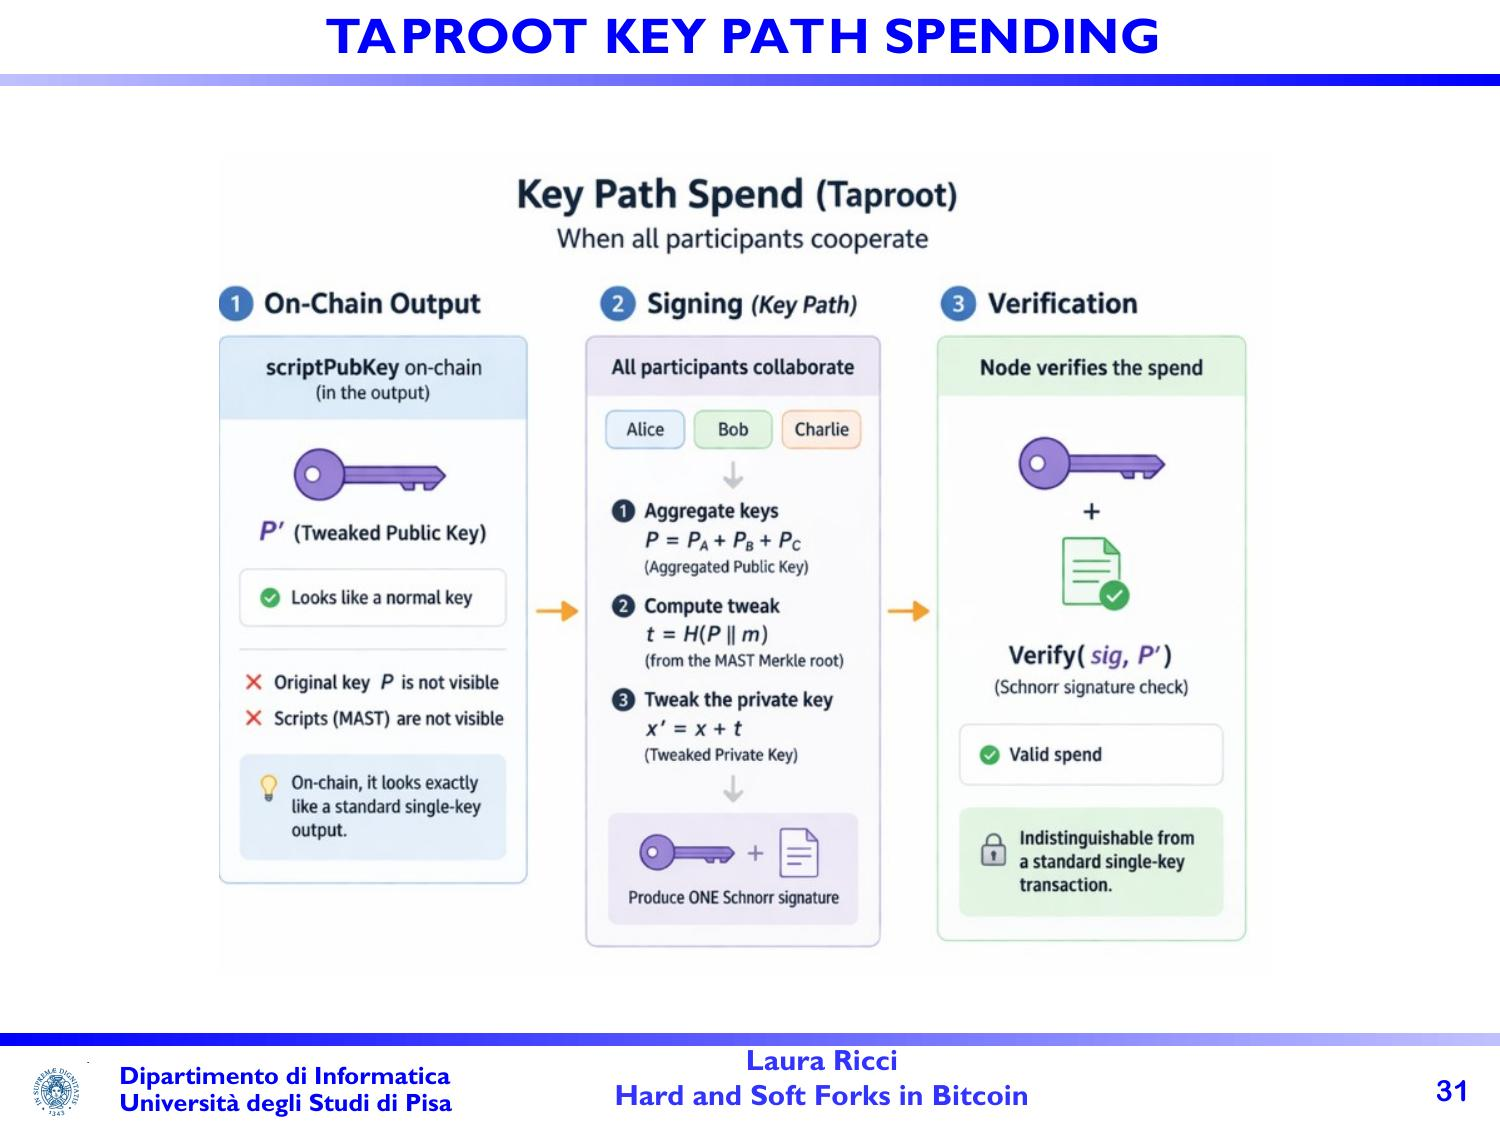
\includegraphics[keepaspectratio,alt={Taproot key path spending: on-chain output con P' (tweaked), firma aggregata di Alice+Bob+Charlie, verifica come singola firma Schnorr}]{images/lezione-18-hard-and-soft-forks-in-bitcoin-img-11.jpg}}
\emph{Fig. --- Key path spending: tutti i partecipanti cooperano,
producono una firma Schnorr aggregata. Il nodo verifica \(\text{sig}\)
rispetto a \(P'\). Indistinguibile da una transazione standard.}

\textbf{Script path spending} (\emph{spesa via script}): se le parti non
possono usare la key path (es. una parte non è disponibile), si rivela
la foglia dello script desiderato e la Merkle proof che dimostra che
quella foglia era nell'albero. Le condizioni alternative rimangono
nascoste.

\pandocbounded{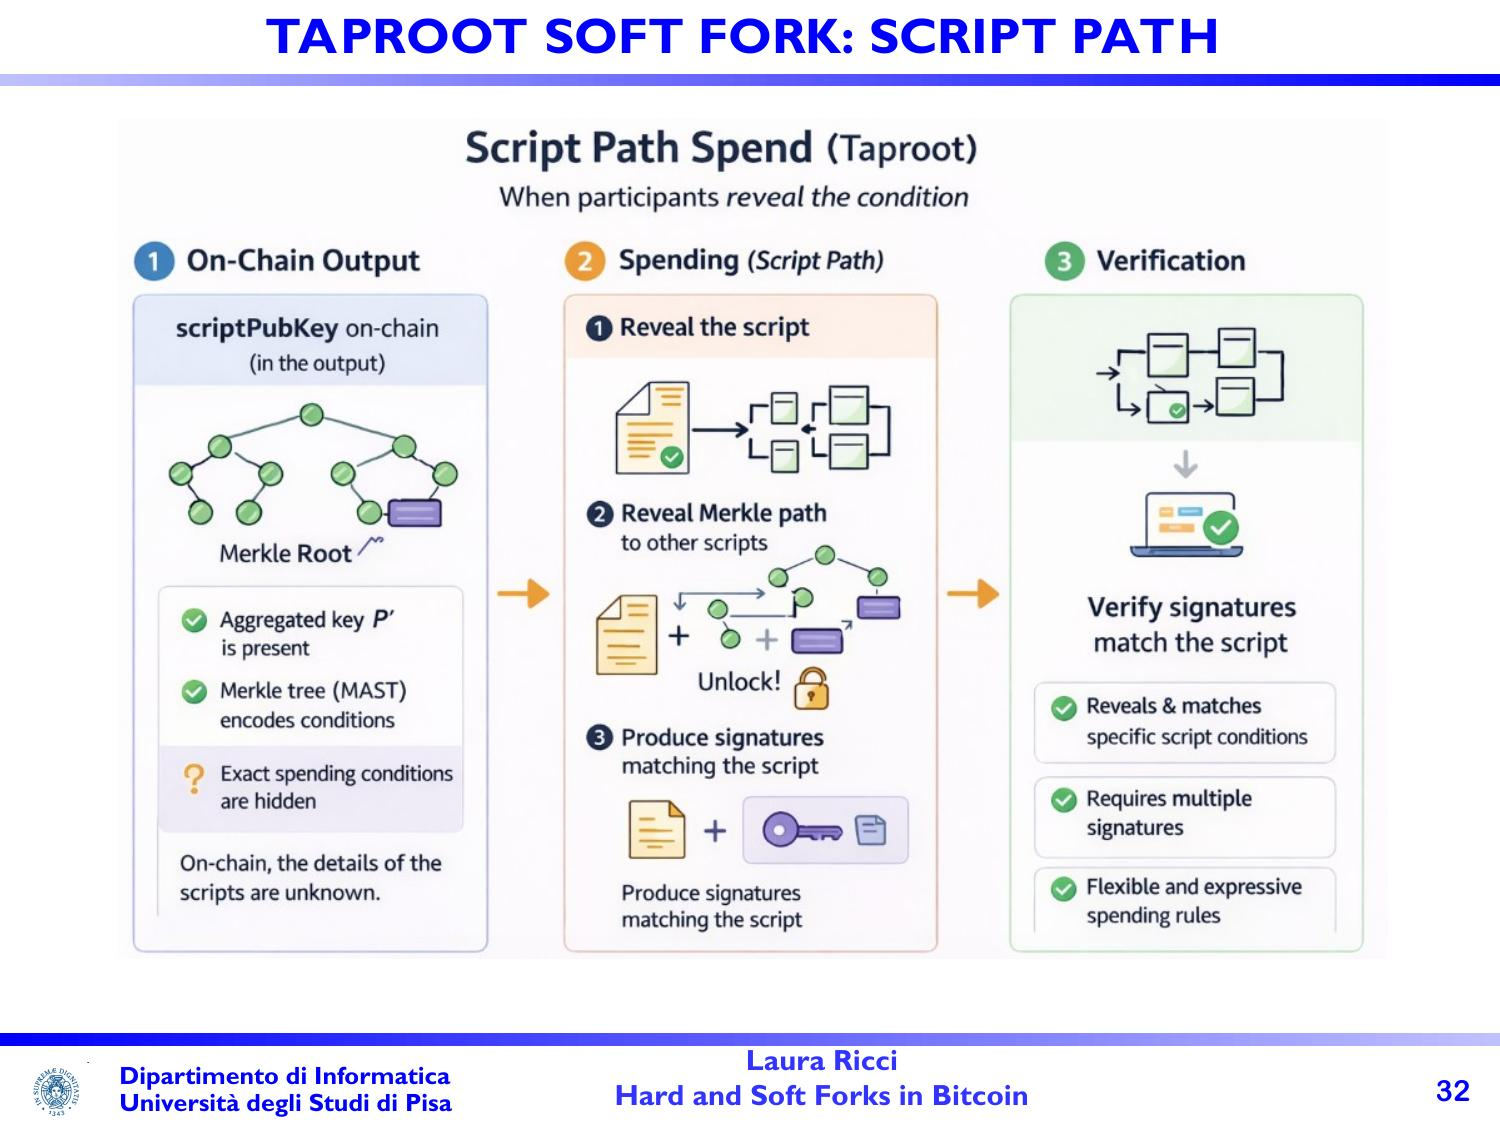
\includegraphics[keepaspectratio,alt={Taproot script path spending: reveal script + Merkle path, produzione firme matching lo script, verifica con controllo condizioni specifiche}]{images/lezione-18-hard-and-soft-forks-in-bitcoin-img-12.jpg}}
\emph{Fig. --- Script path spending: si rivela lo script specifico
(tapleaf) e il Merkle path verso la root. Si producono le firme/dati
richiesti dallo script. Le altre condizioni rimangono private.}

\begin{calloutnote}{Sintesi: Taproot}

Taproot unifica in modo elegante tre tecnologie: Schnorr Signatures
(efficienza e aggregazione), MAST (script privati e compatti), e la
tweaked key (un unico valore on-chain che impegna tutto). Il risultato è
che transazioni Bitcoin complesse --- multisig, timelock, contratti ---
appaiono on-chain identiche a transazioni semplici, migliorando sia la
privacy degli utenti che l'efficienza della rete.

\end{calloutnote}

\begin{center}\rule{0.5\linewidth}{0.5pt}\end{center}

\section{Hard Fork}\label{hard-fork}

\begin{calloutdefinition}{Hard Fork}

Un hard fork è una modifica alle regole di consenso \textbf{non
retrocompatibile} che crea una divisione permanente della blockchain. I
nodi non aggiornati rifiutano i blocchi prodotti dai nodi aggiornati,
portando a due catene distinte.

\end{calloutdefinition}

Le caratteristiche chiave sono: i nodi devono aggiornarsi per seguire le
nuove regole; i nodi vecchi rifiutano i nuovi blocchi, causando una
divisione della catena; le due catene condividono la storia fino al
punto di fork; il risultato è l'esistenza di due reti separate con asset
separati.

\subsection{Bitcoin Cash --- Agosto
2017}\label{bitcoin-cash-agosto-2017}

Il caso più celebre di hard fork di Bitcoin è \textbf{Bitcoin Cash},
nata nell'agosto 2017 dallo stesso giorno in cui veniva attivato SegWit.
Il conflitto alla radice era la scalabilità: come rendere Bitcoin capace
di gestire più transazioni al secondo?

Due visioni si scontrarono. \textbf{Bitcoin Core} sosteneva di mantenere
blocchi piccoli (\textasciitilde1 MB) e di costruire soluzioni di
secondo livello come SegWit e la Lightning Network. \textbf{Bitcoin
Cash} optava per aumentare direttamente la dimensione dei blocchi a 8 MB
e oltre.

L'hard fork ebbe un effetto immediato e interessante: chiunque avesse 10
BTC al momento del fork si ritrovò con 10 BTC e 10 BCH. La chiave
privata Bitcoin funziona anche per Bitcoin Cash, perché le due
blockchain condividono la storia fino al punto di scissione. Gli
indirizzi dei wallet sono gli stessi. Gli UTXO esistenti al momento del
fork sono validi su entrambe le catene, e spendere un UTXO su una catena
non lo consuma sull'altra, perché le due catene sono indipendenti.

\begin{calloutnote}{Stato attuale di Bitcoin Cash}

Bitcoin Cash è ancora attiva. Fornisce circa 200 transazioni al secondo.
Mantiene lo stesso algoritmo di mining di Bitcoin, quindi i miner
possono minare entrambe le criptovalute. Il suo prezzo ha raggiunto un
picco nella fase iniziale per poi calare significativamente rispetto a
Bitcoin.

\end{calloutnote}

\subsection{Hard Fork come Strategia di
Bootstrap}\label{hard-fork-come-strategia-di-bootstrap}

Gli hard fork sono diventati anche uno strumento strategico per lanciare
nuove criptovalute. Anziché costruire una blockchain da zero --- con la
difficoltà di attirare utenti e sviluppatori --- si crea un hard fork di
Bitcoin e si annuncia agli utenti Bitcoin esistenti che riceveranno la
stessa quantità della nuova criptovaluta. Questo abbassa la barriera
all'adozione: chi aveva BTC si ritrova automaticamente con asset nella
nuova rete.

Gli \textbf{Altcoin} sono nati così: alcune sono fork di Bitcoin fatte
da comunità diverse che volevano seguire un percorso alternativo di
sviluppo, altre sono fork nate esplicitamente per creare nuovi asset.

\pandocbounded{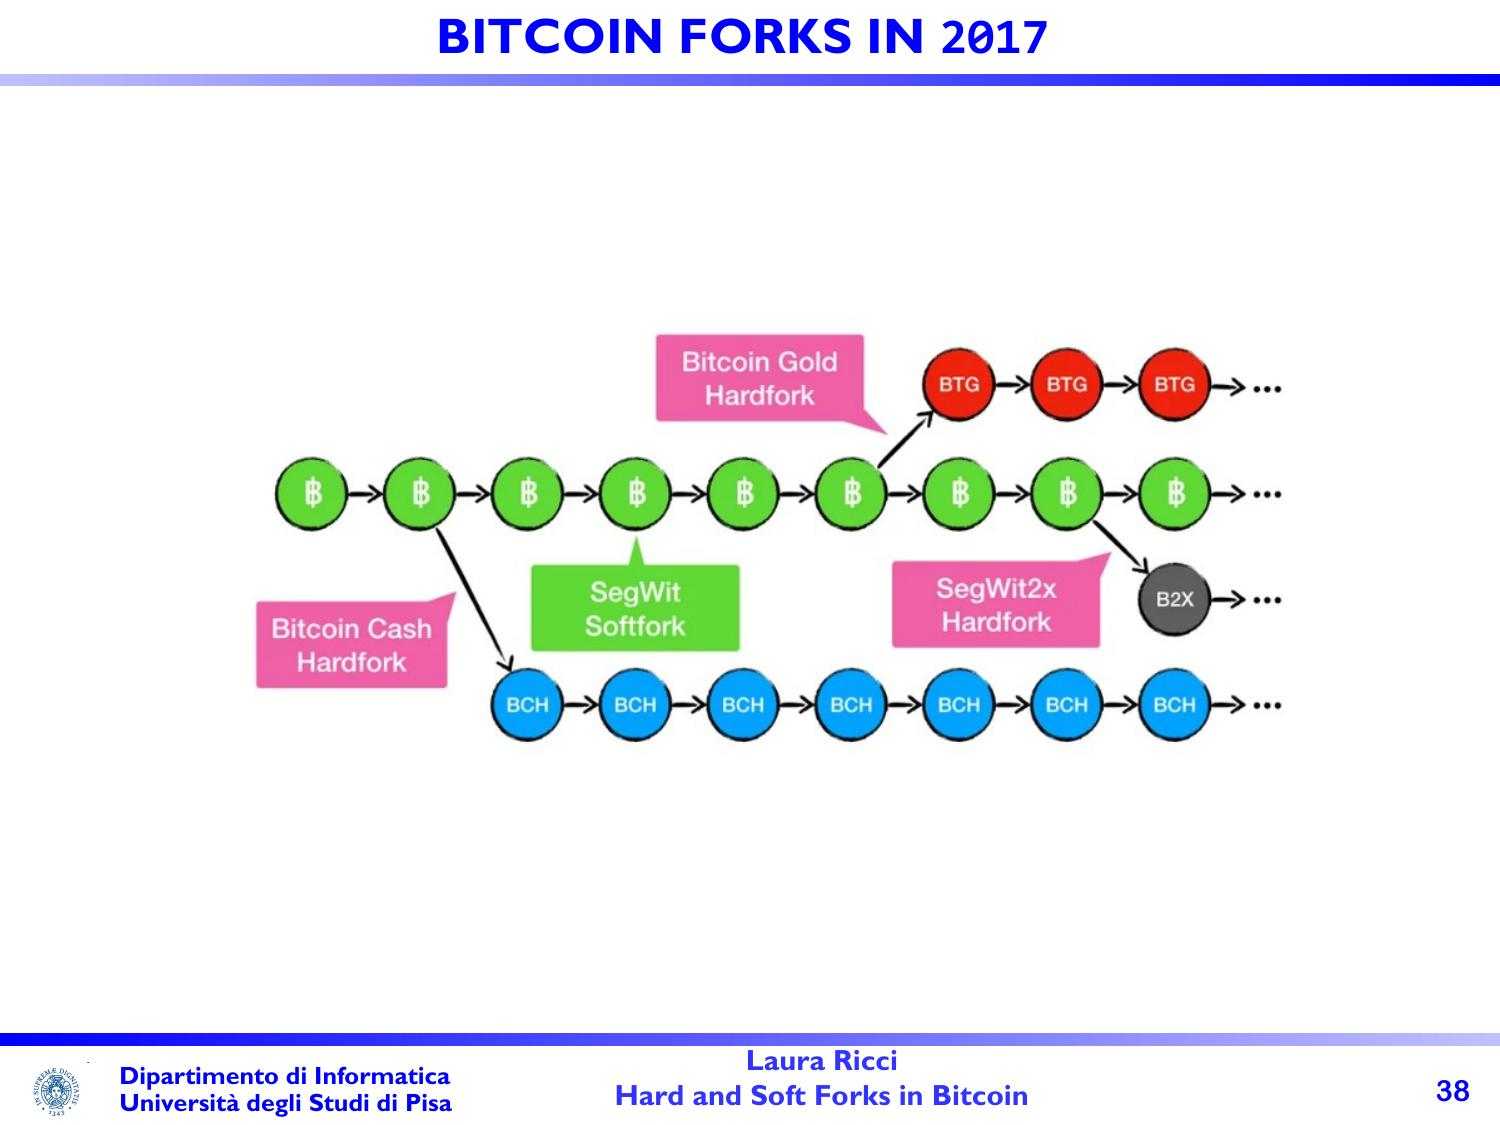
\includegraphics[keepaspectratio,alt={Diagramma dei fork di Bitcoin nel 2017: Bitcoin Cash (hard fork), SegWit (soft fork), SegWit2x (hard fork), Bitcoin Gold (hard fork)}]{images/lezione-18-hard-and-soft-forks-in-bitcoin-img-13.jpg}}
\emph{Fig. --- I fork di Bitcoin nel 2017: Bitcoin Cash e Bitcoin Gold
sono hard fork che generano nuove catene (BCH, BTG); SegWit è il soft
fork che mantiene la catena principale; SegWit2x è un tentativo di hard
fork abortito (B2X).}

\subsection{Hard Fork per Vulnerabilità
Crittografiche}\label{hard-fork-per-vulnerabilituxe0-crittografiche}

Esistono scenari in cui un hard fork non è una scelta ma una necessità
tecnica. Se viene scoperta una vulnerabilità critica nelle primitive
crittografiche usate dalla blockchain, la risposta può richiedere un
hard fork.

Un esempio concreto: se SHA-256 venisse compromesso, Bitcoin dovrebbe
migrare a SHA-3. Aggiungere SHA-3 potrebbe essere un soft fork, ma
rimuovere SHA-2 e sostituirlo completamente con SHA-3 richiede un hard
fork --- è una modifica non retrocompatibile.

Il caso più rilevante a lungo termine è quello dei \textbf{computer
quantistici}: algoritmi come Shor possono rompere la crittografia a
curva ellittica e le firme digitali --- incluse le Schnorr Signatures.
Se un computer quantistico sufficientemente potente diventasse
disponibile, potrebbe derivare chiavi private dalle chiavi pubbliche e
accedere ai fondi di chiunque. La risposta richiederebbe un hard fork
per adottare algoritmi di firma \textbf{post-quantum} resistenti
all'attacco quantistico.

\newpage

\chapter{Ethereum: Account, Transazioni e
Gas}\label{ethereum-account-transazioni-e-gas}

\section{Smart Contracts: l'idea
originale}\label{smart-contracts-lidea-originale}

Il concetto di \textbf{smart contract} non nasce con Ethereum. Fu Nick
Szabo a formularne l'idea nel 1994, descrivendolo come un protocollo di
transazione computerizzato che esegue i termini di un contratto, con
l'obiettivo di soddisfare condizioni contrattuali comuni, minimizzare
eccezioni (sia dolose che accidentali) e ridurre il bisogno di
intermediari fiduciari.

\begin{calloutdefinition}{Smart Contract}

Un programma informatico che automatizza la logica ``se questo accade,
allora fai quello'' tipica dei contratti tradizionali. Il codice
informatico si comporta in modo prevedibile ed è privo delle sfumature
linguistiche del linguaggio naturale.

\end{calloutdefinition}

La novità fondamentale rispetto a un contratto cartaceo è triplice: il
codice è \textbf{più funzionale}, può \textbf{ridurre i costi}, e
soprattutto tende a \textbf{eliminare l'intermediario fiducioso} (banca,
notaio, assicurazione). La crittografia e i meccanismi di sicurezza
garantiscono che le relazioni algoritmicamente specificabili non possano
essere violate.

\subsection{L'esempio dell'aeroporto}\label{lesempio-dellaeroporto}

L'esempio didattico classico è quello assicurativo: Bob è in aeroporto e
il suo volo subisce un ritardo. L'assicurazione ha caricato su una
blockchain (per esempio Ethereum) uno smart contract che monitora i
ritardi dei voli collegandosi al database della compagnia. Non appena la
condizione ``ritardo ≥ X ore'' viene verificata, il contratto accredita
automaticamente l'importo assicurato nel wallet di Bob.

Il meccanismo si articola in tre fasi distinte. Prima, il contratto
viene \textbf{creato} con i termini e le condizioni, e registrato in un
blocco della blockchain tenendo fermi i fondi della compagnia
assicurativa finché la condizione non si avvera. Poi il contratto viene
\textbf{eseguito} da tutti i nodi della rete P2P, che prelevano i dati
dal database dei voli: tutti i nodi devono convergere allo stesso
risultato. Infine, se la maggioranza dei nodi onesti valuta la
condizione come vera, la compensazione viene trasferita automaticamente
a Bob.

\begin{center}\rule{0.5\linewidth}{0.5pt}\end{center}

\section{Perché Bitcoin non basta: i limiti degli
script}\label{perchuxe9-bitcoin-non-basta-i-limiti-degli-script}

Prima di capire cosa fa Ethereum, è utile capire cosa non riesce a fare
Bitcoin. Il linguaggio di scripting di Bitcoin presenta tre limitazioni
strutturali:

\begin{itemize}
\tightlist
\item
  \textbf{Non è Turing-completo}: mancano i cicli, quindi i programmi
  esprimibili sono solo un sottoinsieme finito di computazioni.
\item
  \textbf{Nessuna variabile di stato persistente}: gli script Bitcoin
  consumano i propri input per produrre un output, ma non lasciano
  alcuno stato residuo. Un contratto che ha bisogno di ``ricordare''
  informazioni tra un'esecuzione e l'altra è impossibile da
  implementare.
\item
  \textbf{Cecità verso la blockchain}: gli script non possono accedere
  ai valori degli header dei blocchi (nonce, timestamp, hash del blocco
  precedente).
\end{itemize}

\begin{callouttip}{Intuizione chiave}

Bitcoin è uno storage distribuito di transazioni. Ethereum estende
questo modello trasformando la blockchain in un \textbf{computer
distribuito}: non solo lo storage è replicato, ma anche la computazione.
I nodi non si limitano a validare transazioni, eseguono codice.

\end{callouttip}

\begin{center}\rule{0.5\linewidth}{0.5pt}\end{center}

\section{Ethereum in breve: il world
computer}\label{ethereum-in-breve-il-world-computer}

Ethereum è una piattaforma blockchain per la costruzione di
\textbf{applicazioni decentralizzate} (\emph{DApps}). Fu ideata da
\textbf{Vitalik Buterin} (nato il 31 gennaio 1994) e lanciata nel 2015.

A differenza di Bitcoin, in Ethereum: - il \textbf{codice} delle
applicazioni e il loro \textbf{stato} sono memorizzati sulla blockchain,
- le \textbf{transazioni} non solo trasferiscono criptovaluta, ma
possono innescare l'esecuzione di codice, aggiornare stato, emettere
eventi e scrivere log, - le \textbf{interfacce frontend} possono
rispondere a eventi e leggere log dalla chain.

Le applicazioni di Ethereum vanno ben oltre il semplice trasferimento di
valore: crowdfunding, token (ERC-20), DeFi, NFT, catene di
approvvigionamento, IoT, voto, identità digitale sovrana (SSI). Tra gli
esempi concreti: \emph{Ethereum Name Service}, \emph{Cryptokitties},
exchange decentralizzati.

\begin{calloutnote}{ICO (Initial Coin Offering)}

Un meccanismo basato sul token standard ERC-20 che consente a un'azienda
di raccogliere fondi emettendo nuovi token. Negli anni 2017-2018 gli
investimenti in ICO raggiunsero rispettivamente 7 e 12 miliardi di
dollari.

\end{calloutnote}

\subsection{Ethereum come macchina a stati
distribuita}\label{ethereum-come-macchina-a-stati-distribuita}

Il modello formale di Ethereum è quello di una \textbf{macchina a stati
deterministica distribuita}:

\begin{itemize}
\tightlist
\item
  lo \textbf{stato globale} è l'insieme degli stati di tutti gli smart
  contract,
\item
  le \textbf{transazioni} sono gli eventi che cambiano lo stato globale,
\item
  il \textbf{consenso} garantisce che tutti i nodi concordino sul
  risultato dell'esecuzione e aggiornino il proprio ledger in modo
  coerente.
\end{itemize}

Una proprietà cruciale è il \textbf{determinismo}: lo smart contract
deve produrre lo stesso risultato su ogni nodo. Questo implica che la
logica sia visibile a tutti (trasparenza), ma può creare problemi di
privacy --- risolvibili in alcuni casi con prove a conoscenza zero
(\emph{zero-knowledge proofs}).

\begin{center}\rule{0.5\linewidth}{0.5pt}\end{center}

\section{The Merge: da Proof of Work a Proof of
Stake}\label{the-merge-da-proof-of-work-a-proof-of-stake}

Ethereum nacque con un meccanismo di consenso \textbf{Proof of Work},
identico per principio a quello di Bitcoin. Nel settembre 2022, con
l'evento noto come \textbf{The Merge}, la rete è passata al
\textbf{Proof of Stake}.

\pandocbounded{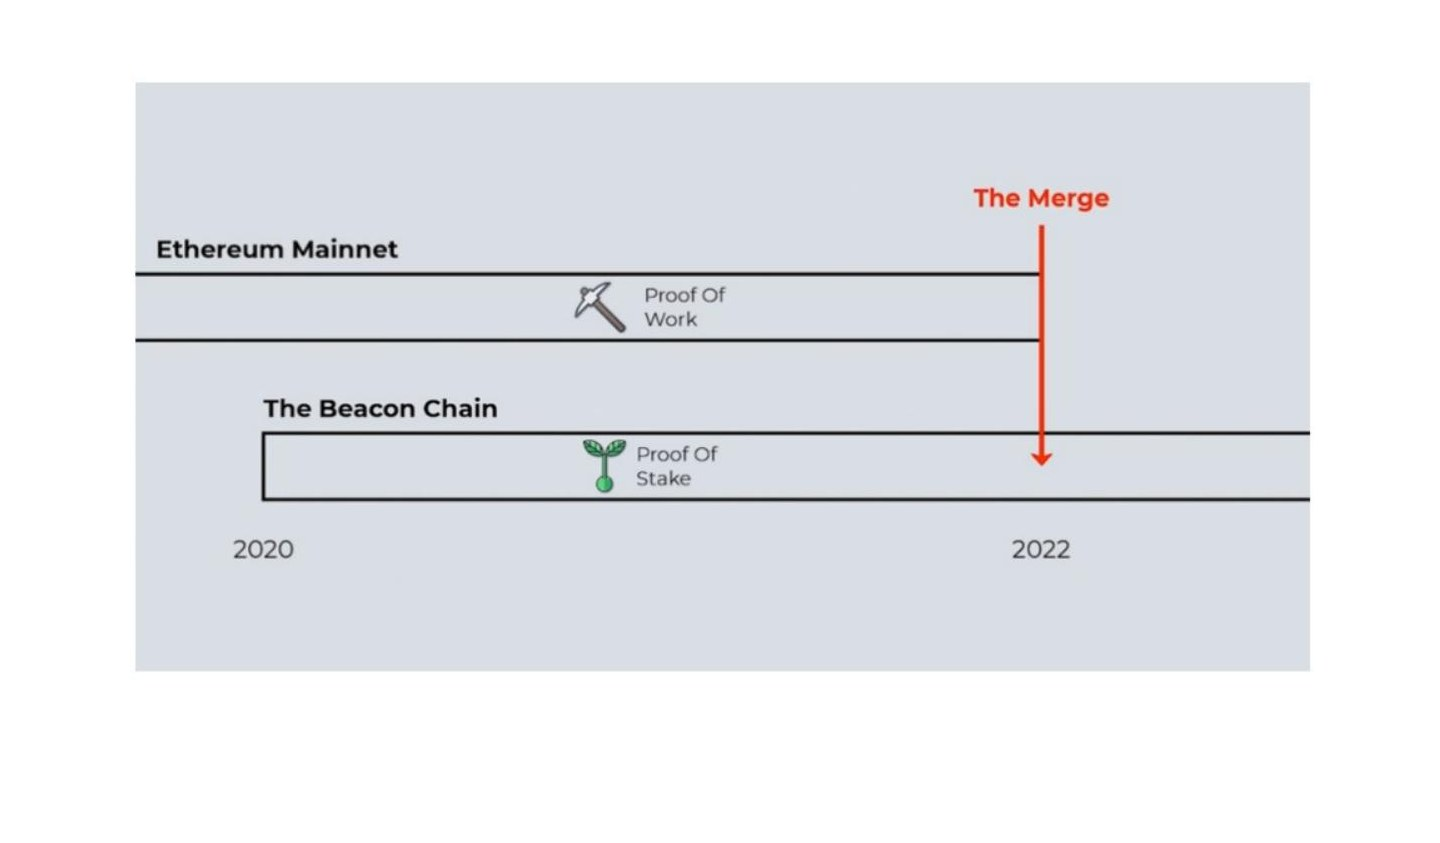
\includegraphics[keepaspectratio,alt={Diagramma del Merge: Ethereum Mainnet e Beacon Chain}]{images/lezione-19-ethereum-accounts-transactions-gas-img-01.jpg}}
\emph{Fig. --- The Merge (settembre 2022): la Ethereum Mainnet (PoW)
converge con la Beacon Chain (PoS), attiva in parallelo dal 2020. Da
quel momento, il consenso è gestito interamente da PoS.}

La transizione era stata preparata con la \textbf{Beacon Chain}, una
chain parallela basata su PoS attiva dal 2020. Al momento del Merge, la
Mainnet PoW si è ``agganciata'' alla Beacon Chain, che da allora
gestisce il consenso.

\begin{center}\rule{0.5\linewidth}{0.5pt}\end{center}

\section{Da Bitcoin a Ethereum: il modello a
stati}\label{da-bitcoin-a-ethereum-il-modello-a-stati}

\subsection{Bitcoin come macchina a stati:
UTXO}\label{bitcoin-come-macchina-a-stati-utxo}

Prima di analizzare Ethereum, vale la pena fissare il modello di Bitcoin
come termine di paragone.

\pandocbounded{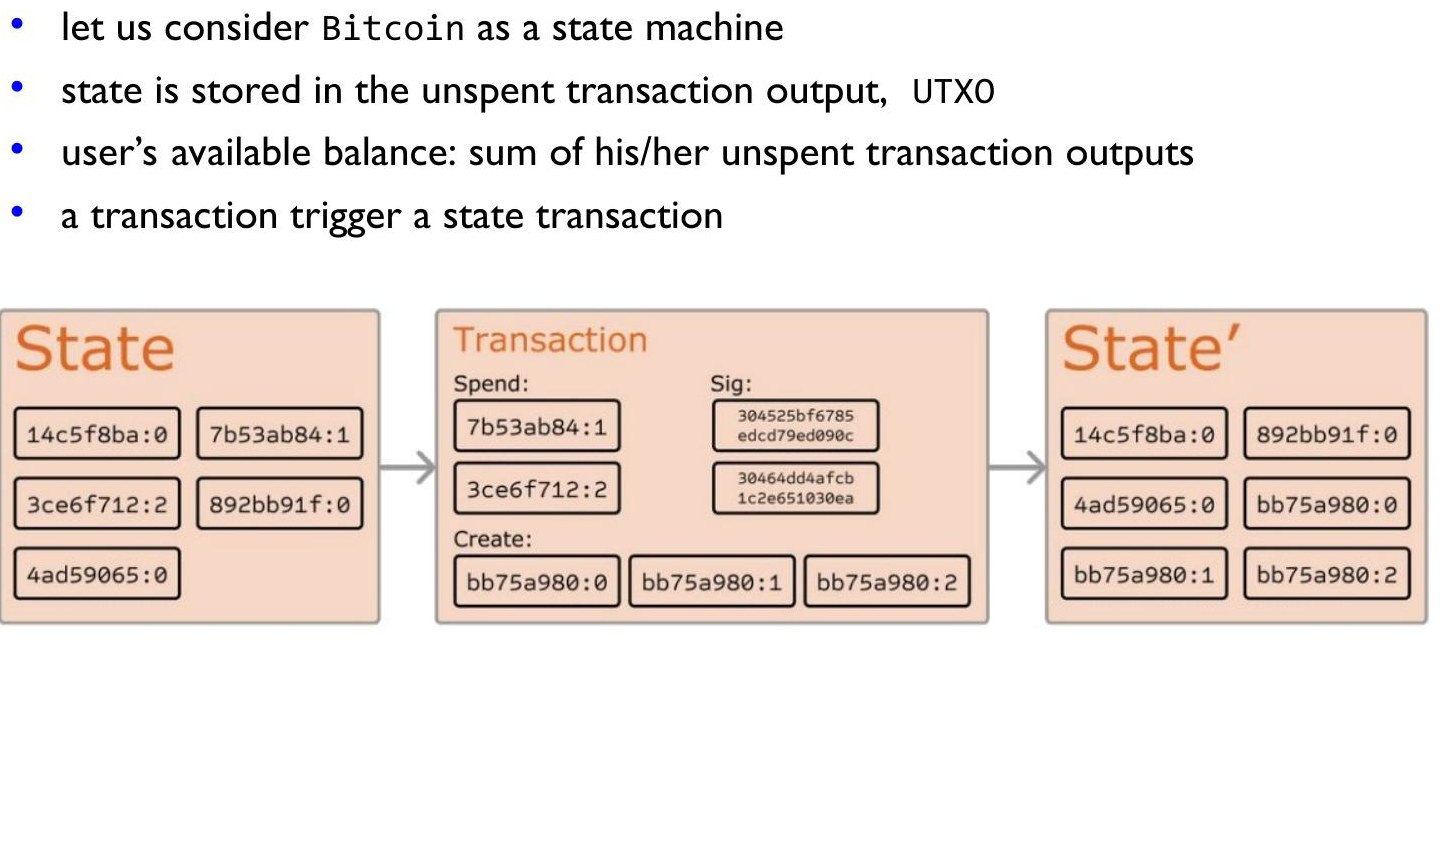
\includegraphics[keepaspectratio,alt={Diagramma della macchina a stati Bitcoin basata su UTXO}]{images/lezione-19-ethereum-accounts-transactions-gas-img-02.jpg}}
\emph{Fig. --- In Bitcoin lo stato è l'insieme degli UTXO (Unspent
Transaction Output). Una transazione consuma degli UTXO esistenti e ne
crea di nuovi, generando la transizione S → S'.}

Il saldo disponibile di un utente Bitcoin è la somma dei suoi UTXO. Ogni
UTXO esiste una sola volta e viene consumato dalla transazione che lo
spende: questo rende impossibile il doppio utilizzo a livello
strutturale.

\subsection{Ethereum: account-based}\label{ethereum-account-based}

Ethereum usa invece un modello \textbf{account-based}, simile a quello
bancario. Lo stato globale non è un insieme di output non spesi, ma un
insieme di \textbf{account}, ognuno con il proprio saldo e, nel caso
degli smart contract, con il proprio codice e storage.

\begin{calloutdefinition}{Ethereum come macchina a stati}

Una macchina virtuale deterministica che applica cambiamenti allo stato
globale replicato. A differenza di Bitcoin, chiunque può definire le
proprie funzioni di transizione di stato tramite smart contract.

\end{calloutdefinition}

\begin{center}\rule{0.5\linewidth}{0.5pt}\end{center}

\section{Gli Account di Ethereum}\label{gli-account-di-ethereum}

Ogni account Ethereum è identificato da un indirizzo di \textbf{20 byte
(160 bit)}. Esistono due tipi fondamentalmente diversi.

\subsection{Externally Owned Account
(EOA)}\label{externally-owned-account-eoa}

Gli \textbf{EOA} sono gli account ``personali'', controllati da
un'entità esterna (persona o organizzazione) tramite una \textbf{chiave
privata}. Chi possiede la chiave privata può accedere ai fondi e
invocare smart contract.

Un EOA contiene: - \textbf{address}: l'indirizzo pubblico dell'account -
\textbf{Ether balance}: il saldo in Ether - \textbf{nonce}: il numero
totale di transazioni emesse da quell'account (da non confondere con il
nonce PoW!)

Un EOA può inviare transazioni per trasferire Ether o per invocare uno
smart contract.

\subsection{Contract Account}\label{contract-account}

Gli account contratto sono controllati non da una chiave privata, ma dal
\textbf{codice} associato. Contengono: - \textbf{contract code}: il
bytecode immutabile del contratto - \textbf{persistent storage}: le
variabili interne del contratto - \textbf{Ether balance}: come gli EOA,
possono ricevere e inviare Ether - \textbf{nonce}: numero di messaggi
inviati da questo account

Gli account contratto \textbf{non hanno chiave privata}: non possono
iniziare autonomamente una transazione, ma solo rispondere a transazioni
o messaggi ricevuti.

\pandocbounded{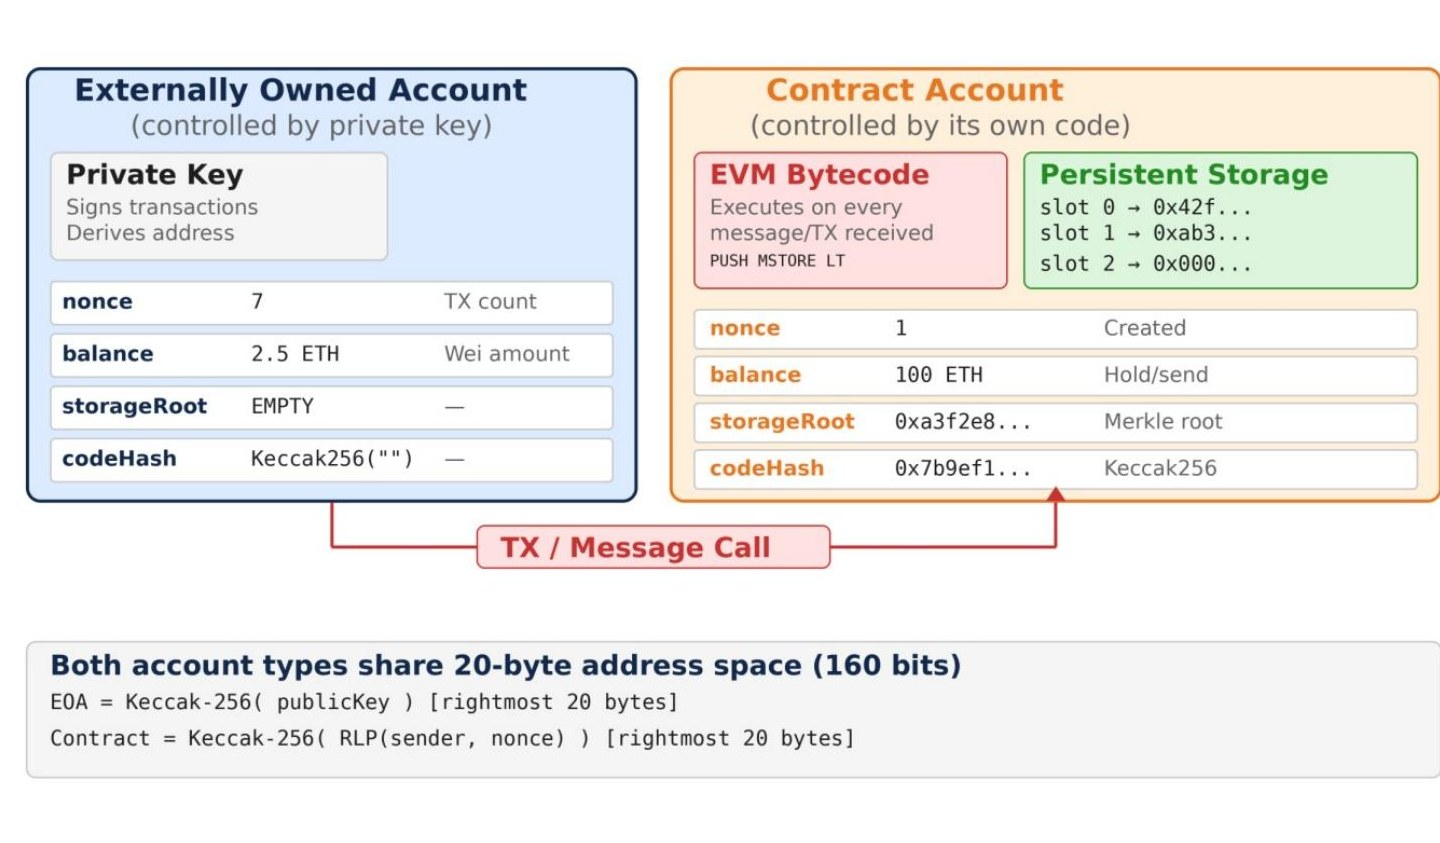
\includegraphics[keepaspectratio,alt={Schema strutturale degli account Ethereum: EOA e Contract Account a confronto}]{images/lezione-19-ethereum-accounts-transactions-gas-img-03.jpg}}
\emph{Fig. --- Confronto strutturale tra EOA e Contract Account. L'EOA
usa una chiave privata per firmare transazioni e ne deriva l'indirizzo
con Keccak-256; il Contract Account espone bytecode EVM e storage
persistente. Entrambi condividono lo spazio di indirizzamento a 20 byte
(160 bit).}

\begin{calloutwarning}{Generazione degli indirizzi}

Per un EOA:
\texttt{EOA\ =\ Keccak-256(publicKey){[}rightmost\ 20\ bytes{]}} Per un
Contract Account:
\texttt{Contract\ =\ Keccak-256(RLP(sender,\ nonce)){[}rightmost\ 20\ bytes{]}}

\end{calloutwarning}

La tabella seguente riassume le differenze operative:

\pandocbounded{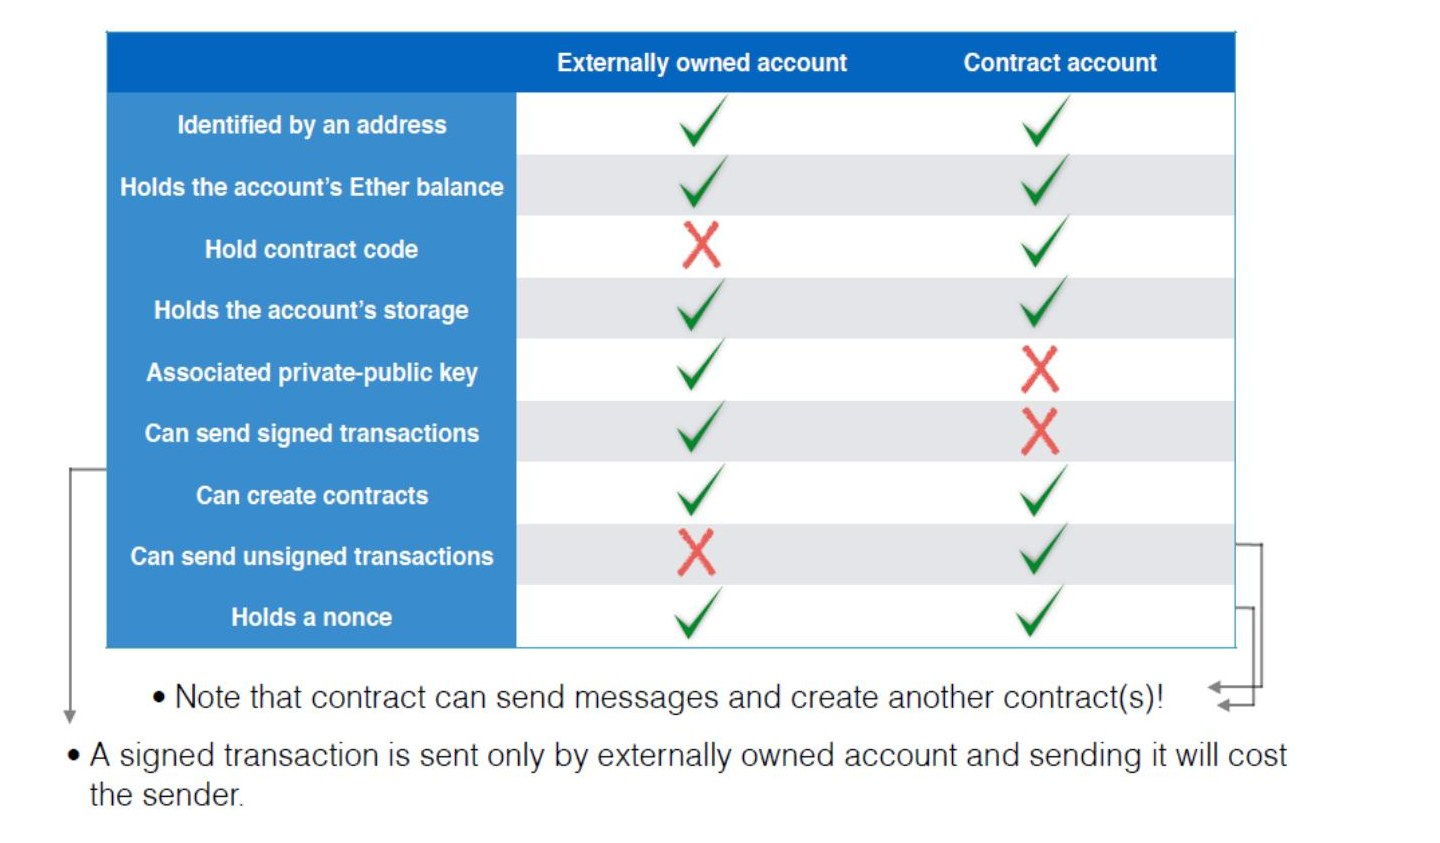
\includegraphics[keepaspectratio,alt={Tabella di confronto tra EOA e Contract Account per caratteristiche}]{images/lezione-19-ethereum-accounts-transactions-gas-img-04.jpg}}
\emph{Fig. --- Confronto delle capacità: solo gli EOA possono inviare
transazioni firmate; solo i Contract Account hanno codice e storage. I
contratti possono inviare messaggi (non transazioni firmate) ad altri
contratti e crearne di nuovi.}

\begin{center}\rule{0.5\linewidth}{0.5pt}\end{center}

\section{Transazioni in Ethereum}\label{transazioni-in-ethereum}

Qualsiasi azione sulla blockchain Ethereum è sempre \textbf{avviata da
una transazione proveniente da un EOA}. Gli EOA sono il ponte tra il
mondo esterno e lo stato interno di Ethereum.

\begin{calloutdefinition}{Transazione}

Un pacchetto dati firmato, serializzato e inviato da un EOA a un altro
account. Può innescare messaggi successivi tra contratti, genera una
modifica allo stato della blockchain se inclusa in un blocco, e può
essere usata per creare nuovi contratti.

\end{calloutdefinition}

\subsection{Transazione EOA → EOA}\label{transazione-eoa-eoa}

La forma più semplice di transazione trasferisce Ether da un EOA a un
altro, funzionalmente analoga a una transazione Bitcoin --- ma basata su
account, non su UTXO.

\pandocbounded{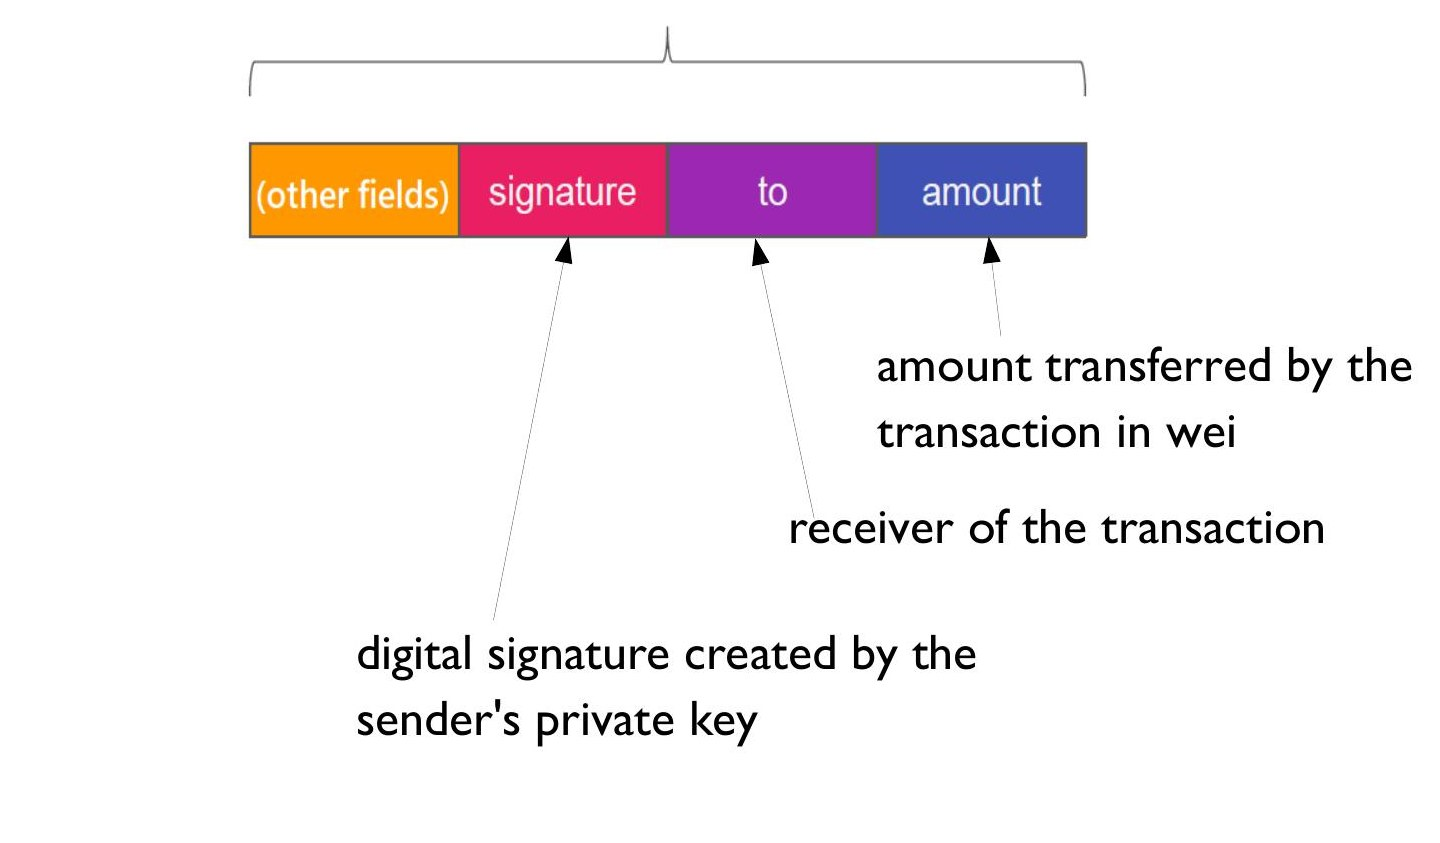
\includegraphics[keepaspectratio,alt={Formato della transazione EOA-to-EOA: campi signature, to, amount}]{images/lezione-19-ethereum-accounts-transactions-gas-img-05.jpg}}
\emph{Fig. --- Formato della transazione EOA→EOA. I campi principali:
\texttt{signature} (firma ECDSA del mittente), \texttt{to} (indirizzo
del destinatario a 20 byte), \texttt{amount} (valore in wei).}

\subsection{Il nonce della
transazione}\label{il-nonce-della-transazione}

\begin{calloutdefinition}{Transaction Nonce}

Un valore scalare uguale al numero di transazioni inviate da
quell'indirizzo (per gli EOA) o al numero di contratti creati (per i
contract account). È un attributo dell'account mittente, non della
singola transazione.

\end{calloutdefinition}

Il nonce serve a due scopi: \textbf{registrare l'ordine delle
transazioni} e \textbf{proteggere dal replay attack}.

\subsubsection{Il replay attack}\label{il-replay-attack}

Il problema nasce dalla differenza strutturale tra Bitcoin ed Ethereum.
In Bitcoin ogni UTXO può essere speso una sola volta: una volta
consumato, sparisce. In Ethereum invece esiste un saldo di account, e la
stessa transazione firmata potrebbe in principio essere ritrasmessa più
volte sulla rete.

Il replay attack funziona così: Alice firma una transazione per inviare
10 ETH a Bob. Bob, dopo che la transazione è stata minata, può prendere
la stessa transazione e ritrametterla ripetutamente, svuotando
progressivamente il conto di Alice.

La soluzione di Ethereum è il nonce: ogni transazione deve includere il
nonce corrente dell'account mittente, e la rete non accetta una seconda
transazione con lo stesso nonce. Bob non può modificare il nonce perché
questo invaliderebbe la firma di Alice.

\begin{calloutwarning}{Ordinamento obbligatorio}

Il nonce impone un ordine rigido. Una transazione con nonce 2 non può
essere minata se la rete non ha già confermato quelle con nonce 0 e 1.
Le transazioni devono essere in sequenza e non possono essere saltate.

\end{calloutwarning}

\begin{center}\rule{0.5\linewidth}{0.5pt}\end{center}

\section{Transizioni di stato in
Ethereum}\label{transizioni-di-stato-in-ethereum}

\subsection{Transizione semplice
EOA→EOA}\label{transizione-semplice-eoaeoa}

\pandocbounded{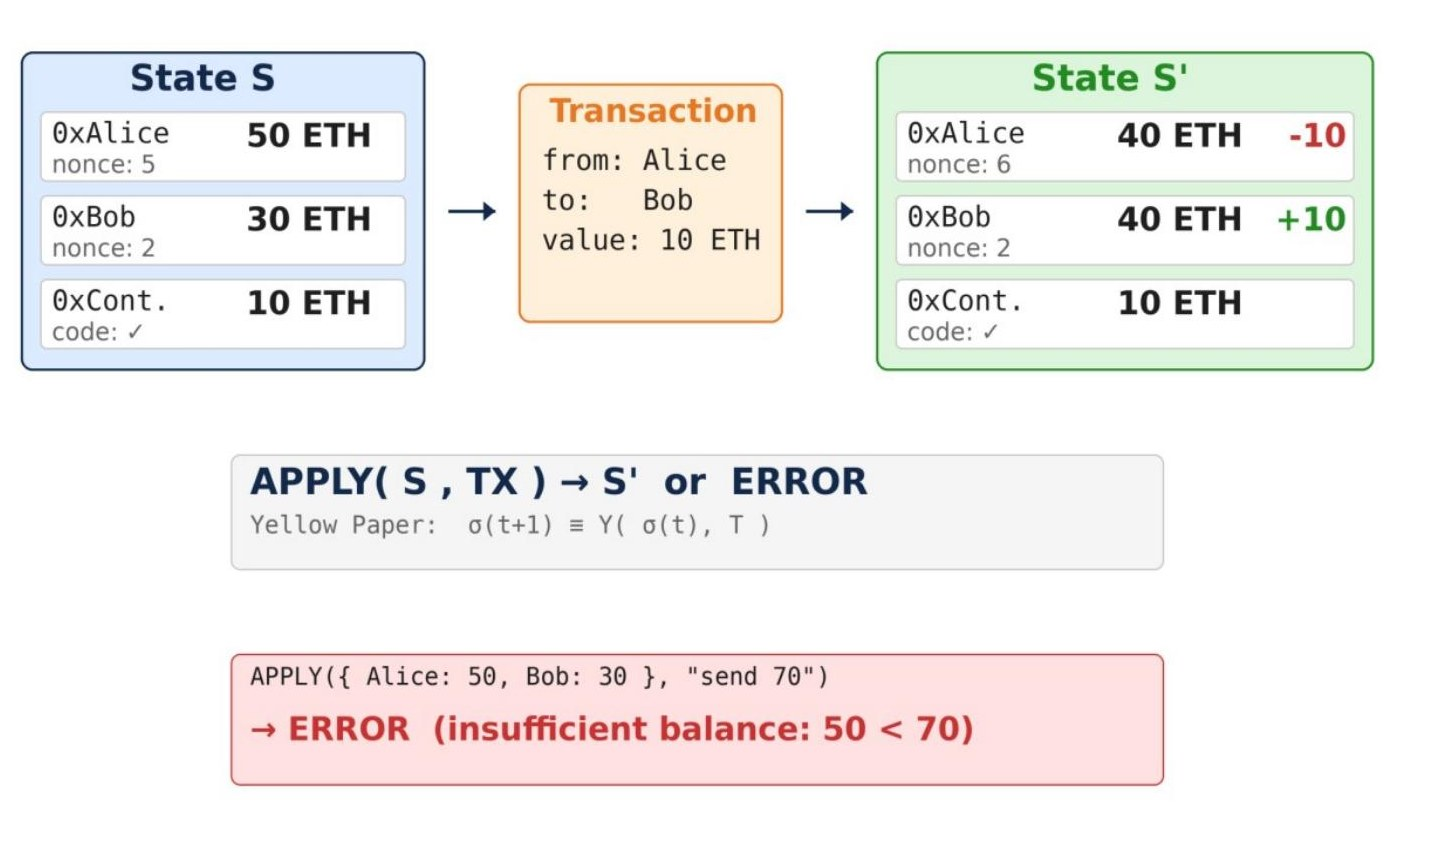
\includegraphics[keepaspectratio,alt={Esempio di transizione di stato tra EOA: Alice invia 10 ETH a Bob}]{images/lezione-19-ethereum-accounts-transactions-gas-img-06.jpg}}
\emph{Fig. --- Transizione di stato EOA→EOA. Alice (50 ETH, nonce 5)
invia 10 ETH a Bob (30 ETH). Lo stato S' vede Alice a 40 ETH (nonce 6) e
Bob a 40 ETH. Se il saldo fosse insufficiente (es. Alice=50, Bob=30,
send 70) la funzione APPLY restituisce ERROR.}

\subsection{Transizione con Smart
Contract}\label{transizione-con-smart-contract}

\pandocbounded{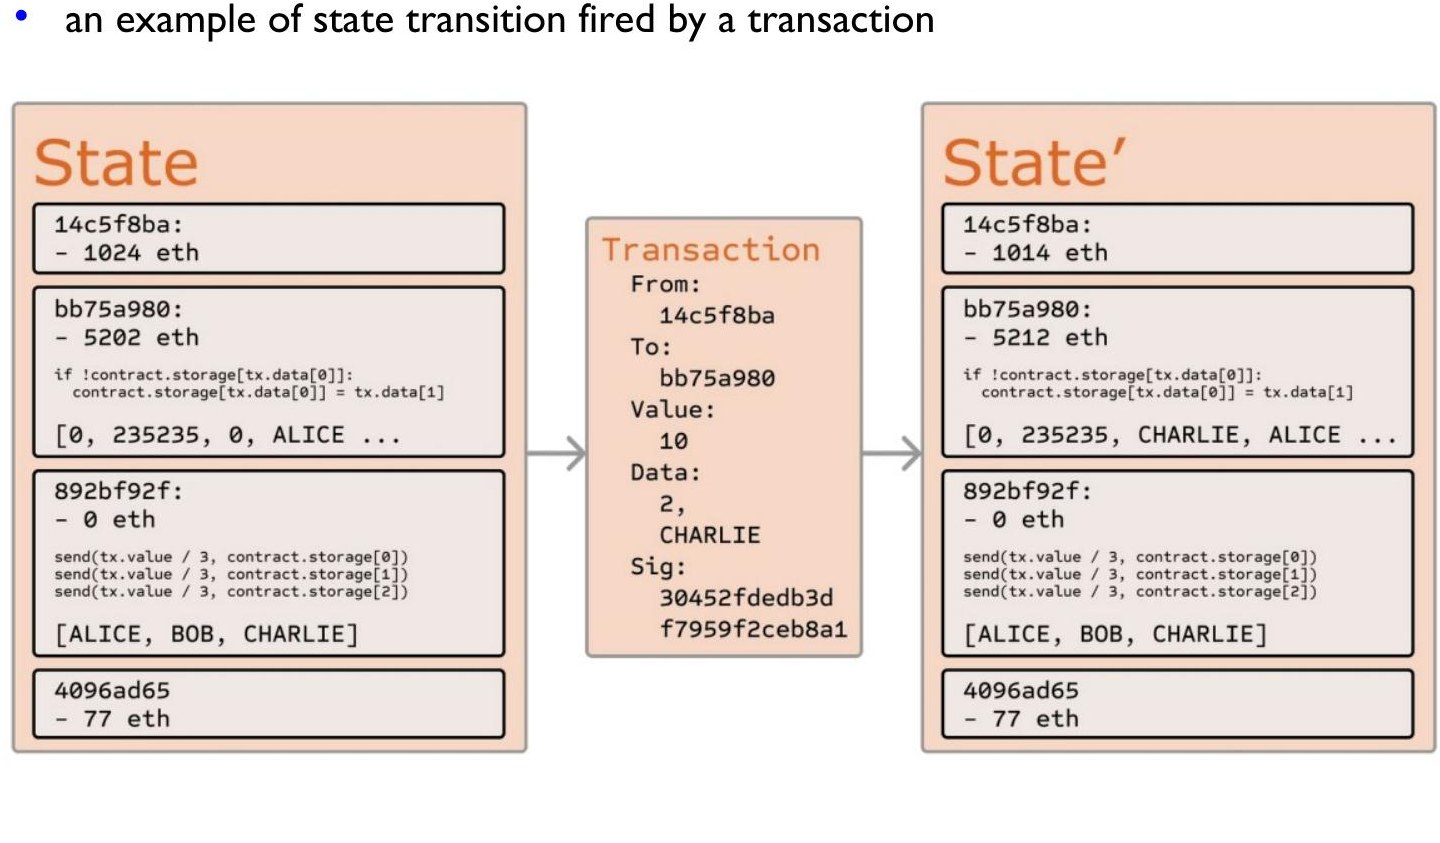
\includegraphics[keepaspectratio,alt={Esempio di transizione di stato con smart contract che aggiorna il proprio storage}]{images/lezione-19-ethereum-accounts-transactions-gas-img-07.jpg}}
\emph{Fig. --- Transizione di stato con contract account. Il mittente
invia una transazione con value 10 e data ``CHARLIE'' al contratto. Il
contratto aggiorna il proprio storage (la lista diventa {[}ALICE, BOB,
CHARLIE{]}) e i saldi vengono aggiornati di conseguenza.}

\begin{center}\rule{0.5\linewidth}{0.5pt}\end{center}

\section{Lifecycle degli Smart
Contract}\label{lifecycle-degli-smart-contract}

Uno smart contract attraversa tre fasi principali:

\pandocbounded{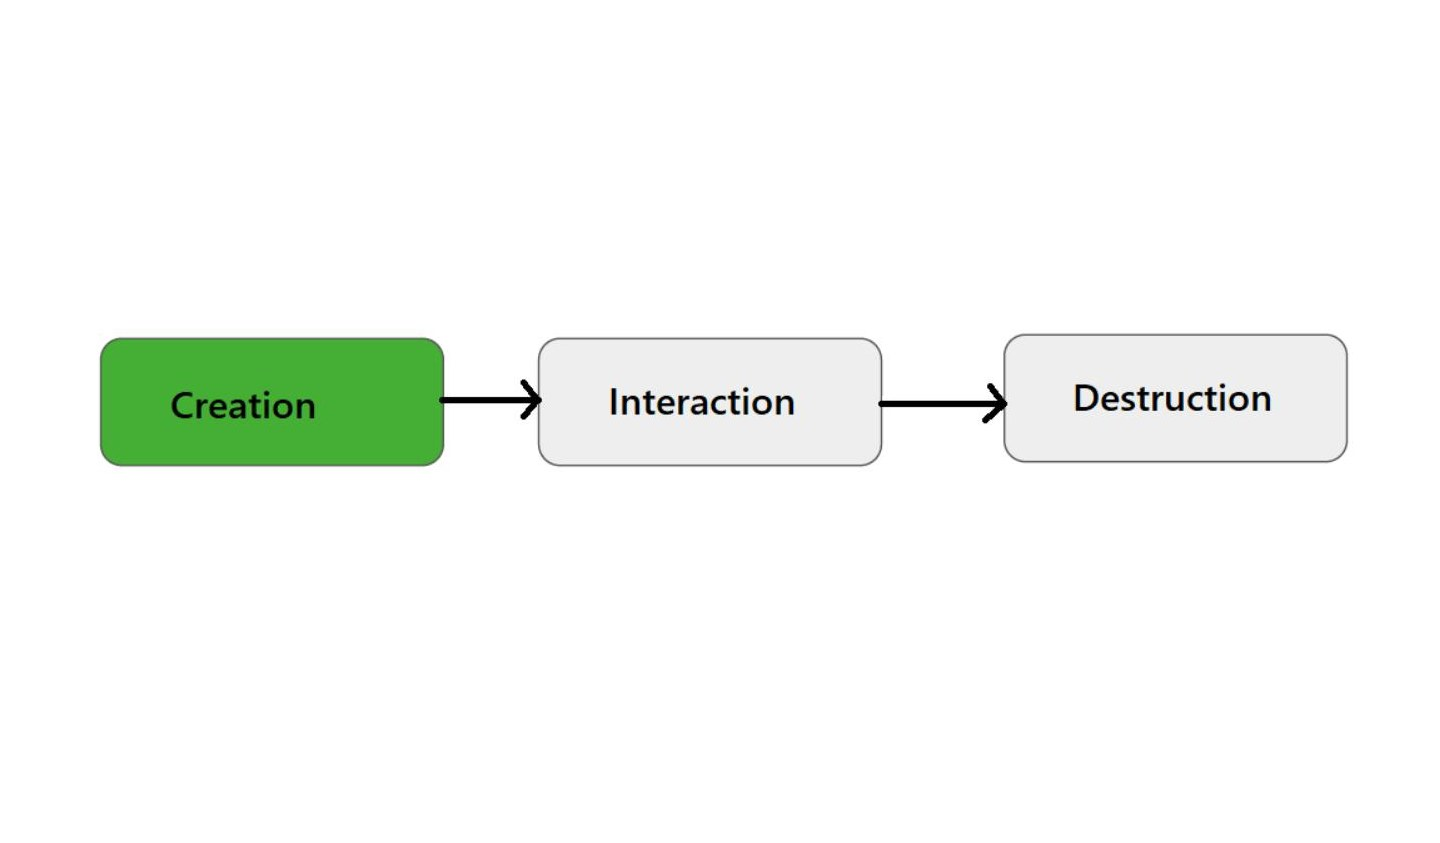
\includegraphics[keepaspectratio,alt={Diagramma del ciclo di vita di uno smart contract: Creation, Interaction, Destruction}]{images/lezione-19-ethereum-accounts-transactions-gas-img-08.jpg}}
\emph{Fig. --- Il lifecycle di uno smart contract è una progressione
lineare: Creazione → Interazione → Distruzione (opzionale).}

\subsection{Creazione}\label{creazione}

Solo un EOA può creare (fare il \emph{deploy} di) uno smart contract
sulla blockchain. La creazione avviene tramite una transazione speciale
in cui il campo \texttt{to} è \textbf{vuoto} (nessun indirizzo di
destinazione finché il contratto non è deployato), e il campo
\texttt{data} contiene il \textbf{bytecode compilato} del contratto.

\pandocbounded{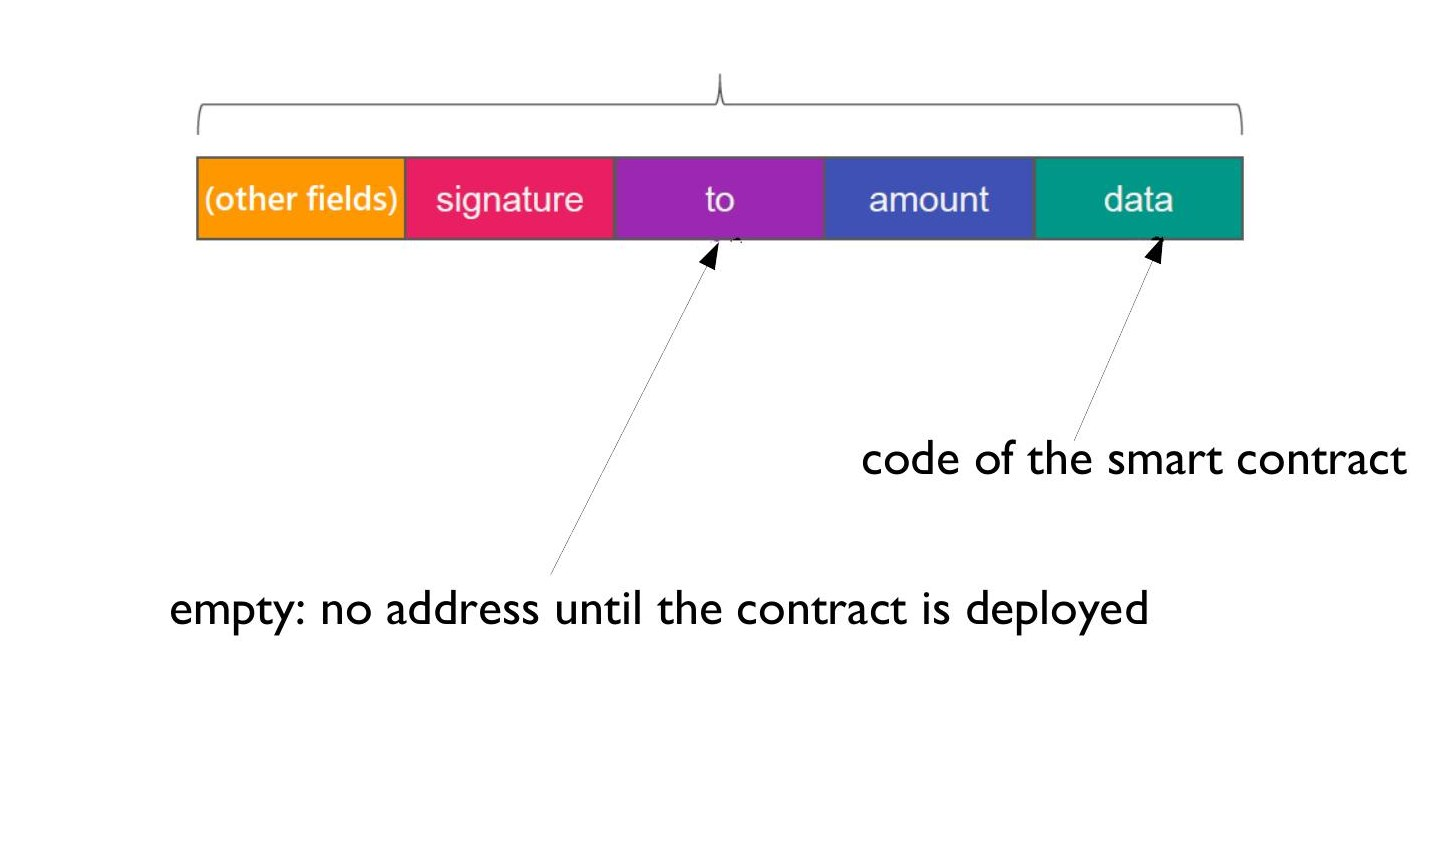
\includegraphics[keepaspectratio,alt={Formato della transazione di creazione contratto: campo to vuoto, data con bytecode}]{images/lezione-19-ethereum-accounts-transactions-gas-img-09.jpg}}
\emph{Fig. --- Transazione di creazione: il campo \texttt{to} è vuoto
(l'indirizzo del contratto viene generato al deploy), il campo
\texttt{data} contiene il bytecode EVM del contratto.}

\subsection{Interazione}\label{interazione}

Una volta deployato, il contratto può essere invocato da: - un
\textbf{EOA} tramite una transazione che specifica l'indirizzo del
contratto e il metodo da chiamare, - un \textbf{altro contratto} tramite
un messaggio interno (non una transazione firmata).

\pandocbounded{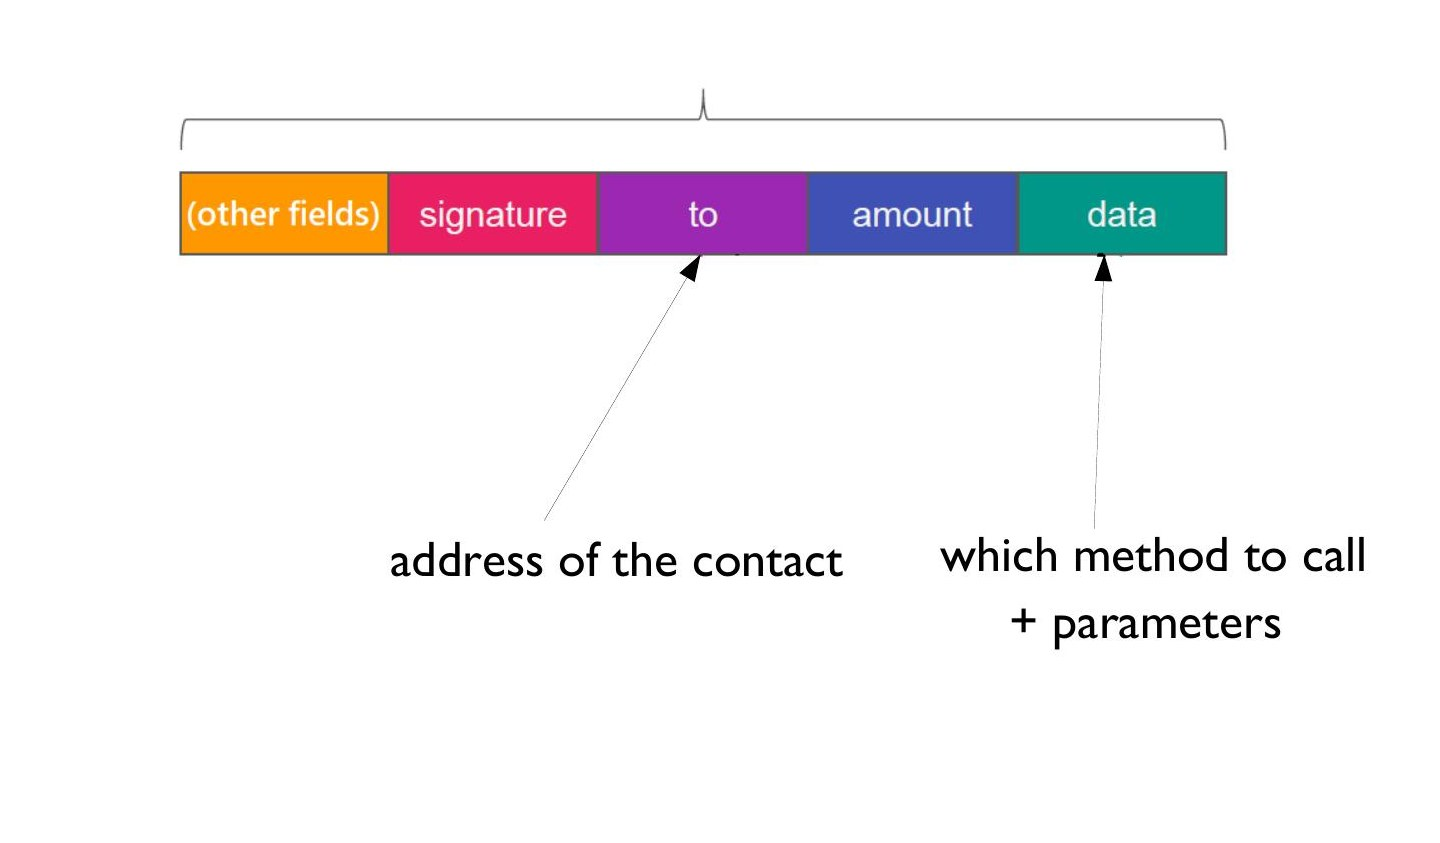
\includegraphics[keepaspectratio,alt={Formato della transazione di interazione con un contratto: to=indirizzo contratto, data=metodo+parametri}]{images/lezione-19-ethereum-accounts-transactions-gas-img-10.jpg}}
\emph{Fig. --- Transazione di interazione: \texttt{to} contiene
l'indirizzo del contratto, \texttt{data} codifica il metodo da invocare
tramite function selector (primi 4 byte del Keccak-256 del prototipo
della funzione) + argomenti ABI-encoded.}

\begin{calloutnote}{Contract-to-Contract}

I contratti non possono avviare transazioni autonomamente, ma possono
costruire percorsi di esecuzione complessi generando \textbf{messaggi}
verso altri contratti come risposta a una transazione ricevuta da un EOA
o da un altro contratto.

\end{calloutnote}

\subsection{Caratteristiche di
esecuzione}\label{caratteristiche-di-esecuzione}

Quando uno smart contract riceve una transazione o un messaggio, viene
eseguito dall'\textbf{Ethereum Virtual Machine (EVM)}. Le azioni
possibili includono: - calcoli aritmetici/logici, - scrittura sullo
storage interno, - invio di messaggi ad altri smart contract, -
creazione di nuovi contratti.

\subsection{Distruzione}\label{distruzione}

Un contratto può essere eliminato dalla blockchain invocando
l'operazione \textbf{\texttt{selfdestruct}}. La transazione di
distruzione contiene nel campo \texttt{data} il nome del metodo che
chiama \texttt{selfdestruct}, e nel campo \texttt{to} l'indirizzo del
contratto. Dopo la distruzione, il contratto non è più eseguibile.

\subsection{Esempio Naive in Solidity}\label{esempio-naive-in-solidity}

\begin{Shaded}
\begin{Highlighting}[]
\NormalTok{pragma solidity \^{}0.8.0;}

\NormalTok{contract Crowdsale \{}
\NormalTok{    mapping(address =\textgreater{} uint256) public balances;}
\NormalTok{    uint256 public totalRaised;}

\NormalTok{    function contribute() public payable \{}
\NormalTok{        require(msg.value \textgreater{} 0, "Contribution amount must be greater than zero");}
\NormalTok{        balances[msg.sender] += msg.value;}
\NormalTok{        totalRaised += msg.value;}
\NormalTok{    \}}

\NormalTok{    function withdraw() public \{}
\NormalTok{        uint256 amount = balances[msg.sender];}
\NormalTok{        require(amount \textgreater{} 0, "No funds available to withdraw");}
\NormalTok{        balances[msg.sender] = 0;}
\NormalTok{        payable(msg.sender).transfer(amount);}
\NormalTok{    \}}
\NormalTok{\}}
\end{Highlighting}
\end{Shaded}

Questo semplice contratto di crowdfunding mostra i meccanismi
fondamentali di Solidity: un \texttt{mapping} per tenere traccia dei
contributi, una funzione \texttt{payable} per ricevere Ether, e una
funzione di prelievo con verifica del saldo e azzeramento prima del
trasferimento (per prevenire reentrancy attack).

\begin{center}\rule{0.5\linewidth}{0.5pt}\end{center}

\section{Il Formato Completo della
Transazione}\label{il-formato-completo-della-transazione}

Ogni transazione Ethereum include i seguenti campi, serializzati con lo
schema \textbf{RLP} (\emph{Recursive Length Prefix}):

\pandocbounded{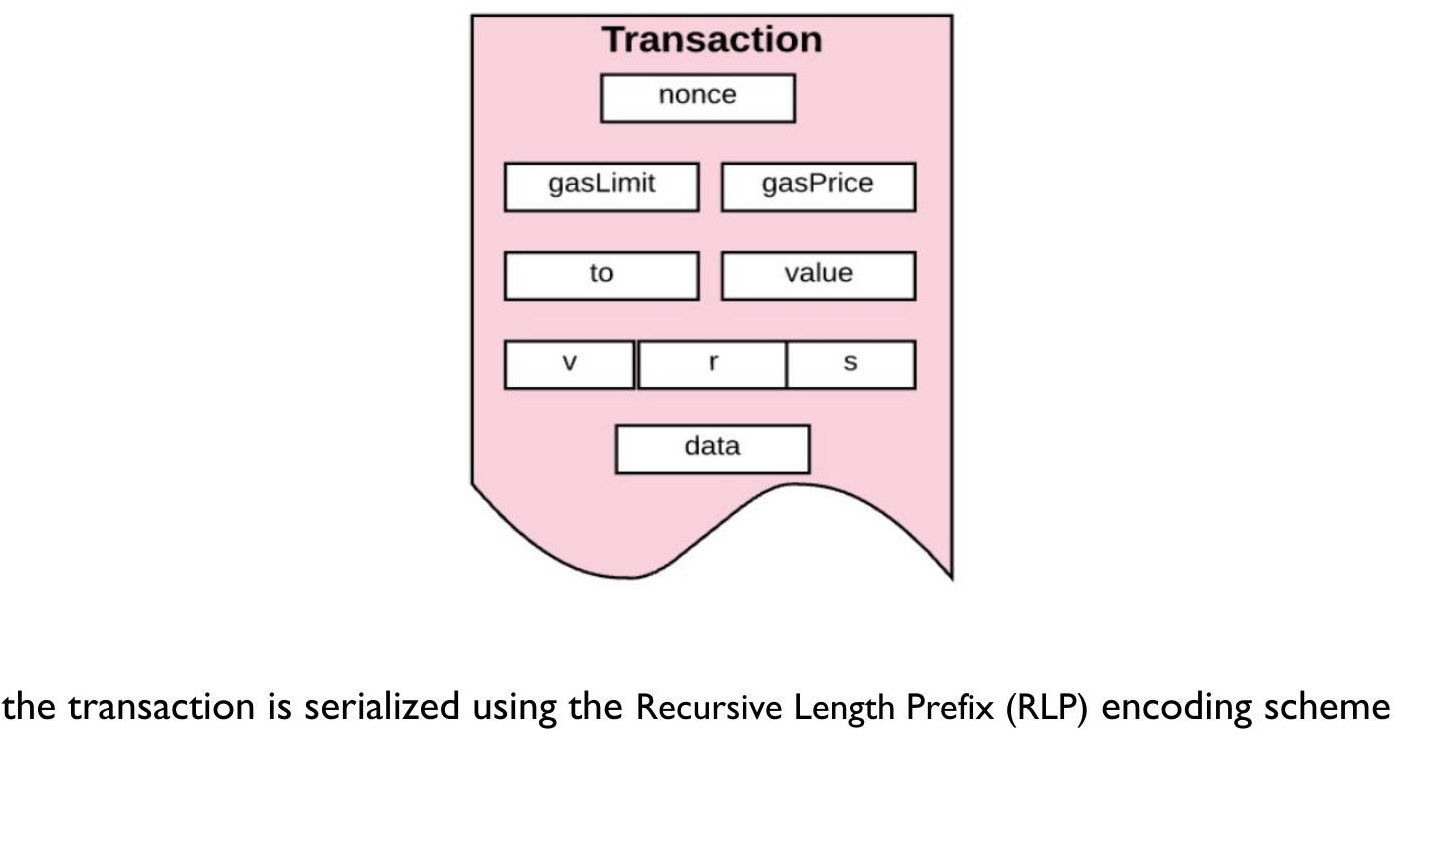
\includegraphics[keepaspectratio,alt={Schema UML del formato completo di una transazione Ethereum}]{images/lezione-19-ethereum-accounts-transactions-gas-img-11.jpg}}
\emph{Fig. --- Struttura completa di una transazione Ethereum: nonce,
gasLimit, gasPrice, to, value, i tre componenti della firma ECDSA (v, r,
s), e data.}

{\def\LTcaptype{none} % do not increment counter
\begin{longtable}[]{@{}
  >{\raggedright\arraybackslash}p{(\linewidth - 2\tabcolsep) * \real{0.3500}}
  >{\raggedright\arraybackslash}p{(\linewidth - 2\tabcolsep) * \real{0.6500}}@{}}
\toprule\noalign{}
\begin{minipage}[b]{\linewidth}\raggedright
Campo
\end{minipage} & \begin{minipage}[b]{\linewidth}\raggedright
Descrizione
\end{minipage} \\
\midrule\noalign{}
\endhead
\bottomrule\noalign{}
\endlastfoot
\texttt{nonce} & Numero progressivo di transazioni dell'EOA mittente \\
\texttt{gasLimit} & Quantità massima di gas che il mittente è disposto a
consumare \\
\texttt{gasPrice} & Prezzo in wei per unità di gas (scelto dal
mittente) \\
\texttt{to} & Indirizzo destinatario (20 byte); vuoto per creazione
contratto \\
\texttt{value} & Importo in wei da trasferire \\
\texttt{v}, \texttt{r}, \texttt{s} & Componenti della firma ECDSA;
permettono di ricavare l'indirizzo del mittente \\
\texttt{data} & Payload: bytecode (creazione) o function selector +
argomenti (interazione) \\
\end{longtable}
}

\subsection{\texorpdfstring{Il campo
\texttt{to}}{Il campo to}}\label{il-campo-to}

Il campo \texttt{to} accetta qualsiasi valore di 20 byte senza
validazione: se l'indirizzo è errato o inesistente, l'Ether inviato
viene \textbf{bruciato} (\emph{burnt}). Rispetto a Bitcoin, Ethereum
semplifica radicalmente il formato: un solo indirizzo di output, valore
inserito direttamente (nessun riferimento a transazione precedente),
nessuno script nel campo destinatario.

\subsection{\texorpdfstring{I campi \texttt{value} e
\texttt{data}}{I campi value e data}}\label{i-campi-value-e-data}

I due campi del payload possono essere combinati in modi diversi:

{\def\LTcaptype{none} % do not increment counter
\begin{longtable}[]{@{}
  >{\raggedright\arraybackslash}p{(\linewidth - 4\tabcolsep) * \real{0.3000}}
  >{\raggedright\arraybackslash}p{(\linewidth - 4\tabcolsep) * \real{0.2667}}
  >{\raggedright\arraybackslash}p{(\linewidth - 4\tabcolsep) * \real{0.4333}}@{}}
\toprule\noalign{}
\begin{minipage}[b]{\linewidth}\raggedright
\texttt{value}
\end{minipage} & \begin{minipage}[b]{\linewidth}\raggedright
\texttt{data}
\end{minipage} & \begin{minipage}[b]{\linewidth}\raggedright
Significato
\end{minipage} \\
\midrule\noalign{}
\endhead
\bottomrule\noalign{}
\endlastfoot
valorizzato & vuoto & Pagamento puro in Ether \\
vuoto & valorizzato & Invocazione di funzione \\
entrambi valorizzati & entrambi valorizzati & Invocazione con
trasferimento Ether \\
\end{longtable}
}

Quando \texttt{data} è inviato a un contract account, i primi \textbf{4
byte} costituiscono il \textbf{function selector} (i primi 4 byte
dell'hash Keccak-256 del prototipo della funzione), che identifica
univocamente il metodo da invocare. I byte successivi codificano gli
argomenti secondo l'ABI Ethereum.

\begin{center}\rule{0.5\linewidth}{0.5pt}\end{center}

\section{Il Problema dell'Halting e il
Gas}\label{il-problema-dellhalting-e-il-gas}

Il prezzo della Turing-completezza è l'\textbf{halting problem}: non è
possibile determinare staticamente se un programma terminerà o girerà
all'infinito. Per verificarlo bisogna eseguirlo --- ma eseguire codice
che non termina su una rete di nodi significa un \textbf{denial of
service} distribuito. Bitcoin non ha questo problema (il suo linguaggio
non è Turing-completo), Ethereum sì.

\begin{Shaded}
\begin{Highlighting}[]
\KeywordTok{function} \FunctionTok{foo}\NormalTok{() \{}
    \ControlFlowTok{while}\NormalTok{ (}\KeywordTok{true}\NormalTok{) \{ }\CommentTok{/* Loop forever! */}\NormalTok{ \}}
\NormalTok{\}}
\end{Highlighting}
\end{Shaded}

\subsection{La soluzione: il Gas}\label{la-soluzione-il-gas}

\begin{calloutdefinition}{Gas}

Un'unità di misura del costo computazionale associato all'esecuzione di
ogni istruzione EVM. Ogni transazione include un budget di gas; l'EVM si
ferma (e la transazione fallisce) non appena il gas si esaurisce.

\end{calloutdefinition}

Il gas serve a tre scopi: 1. \textbf{Rendere costosi gli attacchi DoS}:
chi vuole eseguire codice malevolo deve pagare per ogni ciclo. 2.
\textbf{Compensare i miner/validatori}: le fee di esecuzione
ricompensano chi convalida le transazioni. 3. \textbf{Definire il limite
computazionale}: l'EVM è una macchina \emph{quasi}-Turing-completa ---
può eseguire qualsiasi programma purché disponga di gas sufficiente.

\subsection{Gas Price e Gas Limit}\label{gas-price-e-gas-limit}

La \textbf{gas price} è il prezzo in Ether per unità di gas, espresso in
\textbf{gwei} (1 gwei = 10⁹ wei). È il mittente a sceglierla: alta
priorità richiede alta gas price, poiché i miner preferiscono le
transazioni più remunerative. Il prezzo è variabile e dipende dalla
congestione della rete.

Il \textbf{gas limit} è la quantità massima di gas che il mittente è
disposto a consumare. La fee massima pagabile è:

\[
\text{fee} = \text{gasPrice} \times \text{gasLimit}
\]

Se al termine dell'esecuzione rimane del gas inutilizzato, viene
\textbf{rimborsato} al mittente. Se il gas si esaurisce prima del
completamento, tutte le modifiche di stato vengono \textbf{revertite}
(ma il gas consumato non viene restituito).

\subsection{Ether e le sue
denominazioni}\label{ether-e-le-sue-denominazioni}

\pandocbounded{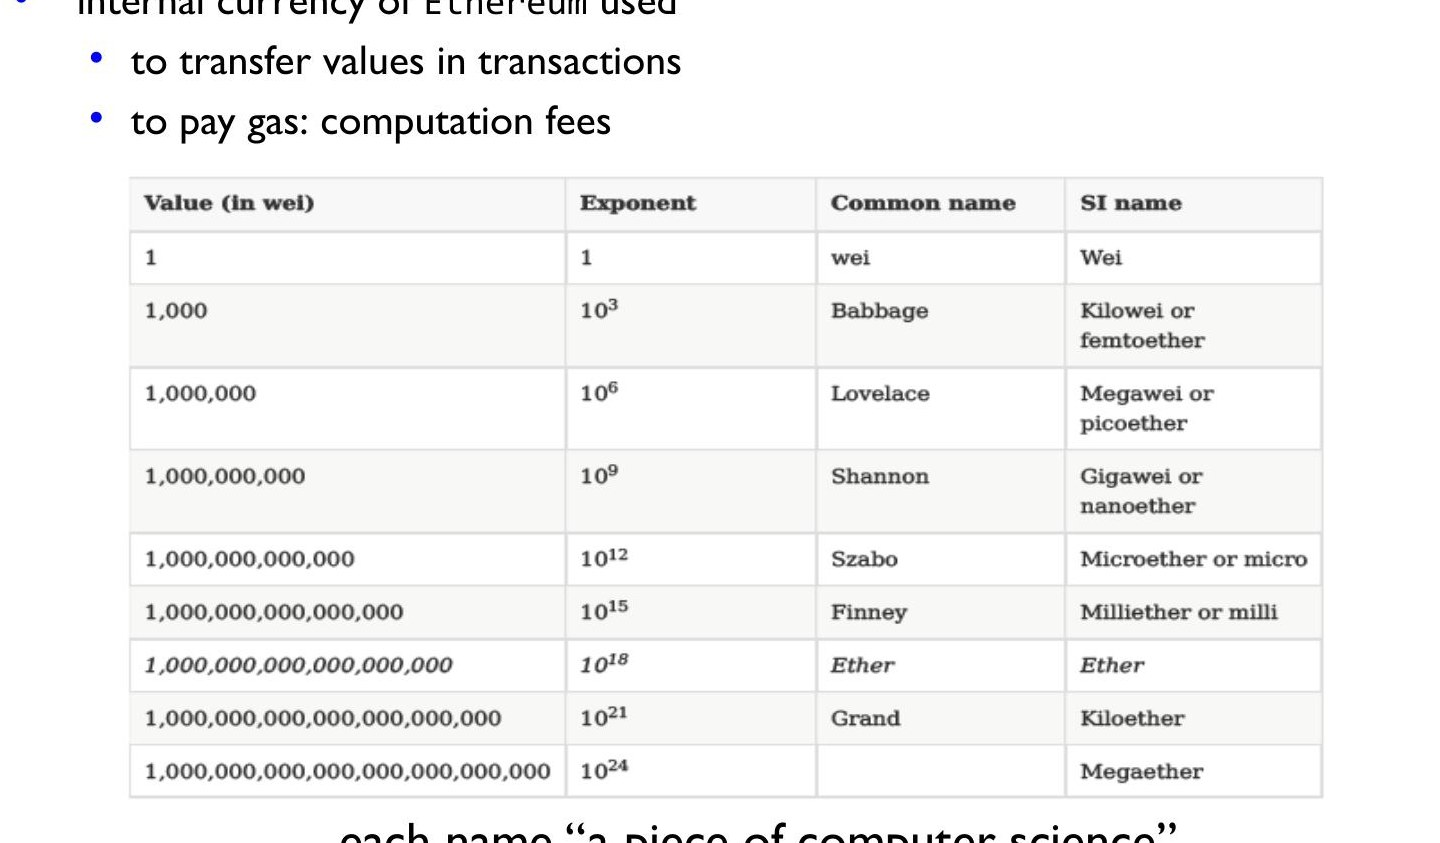
\includegraphics[keepaspectratio,alt={Tabella delle denominazioni dell'Ether: da wei a Megaether}]{images/lezione-19-ethereum-accounts-transactions-gas-img-12.jpg}}
\emph{Fig. --- Le denominazioni dell'Ether, ciascuna intitolata a un
pioniere dell'informatica: wei (unità base), Babbage (10³), Lovelace
(10⁶), Shannon (10⁹), Szabo (10¹²), Finney (10¹⁵), Ether (10¹⁸), Grand
(10²¹), Megaether (10²⁴).}

L'unità base è il \textbf{wei}: 1 ETH = 10¹⁸ wei. Tutte le operazioni
interne di Ethereum lavorano in wei.

\subsection{Il meccanismo del Gas:
riepilogo}\label{il-meccanismo-del-gas-riepilogo}

\pandocbounded{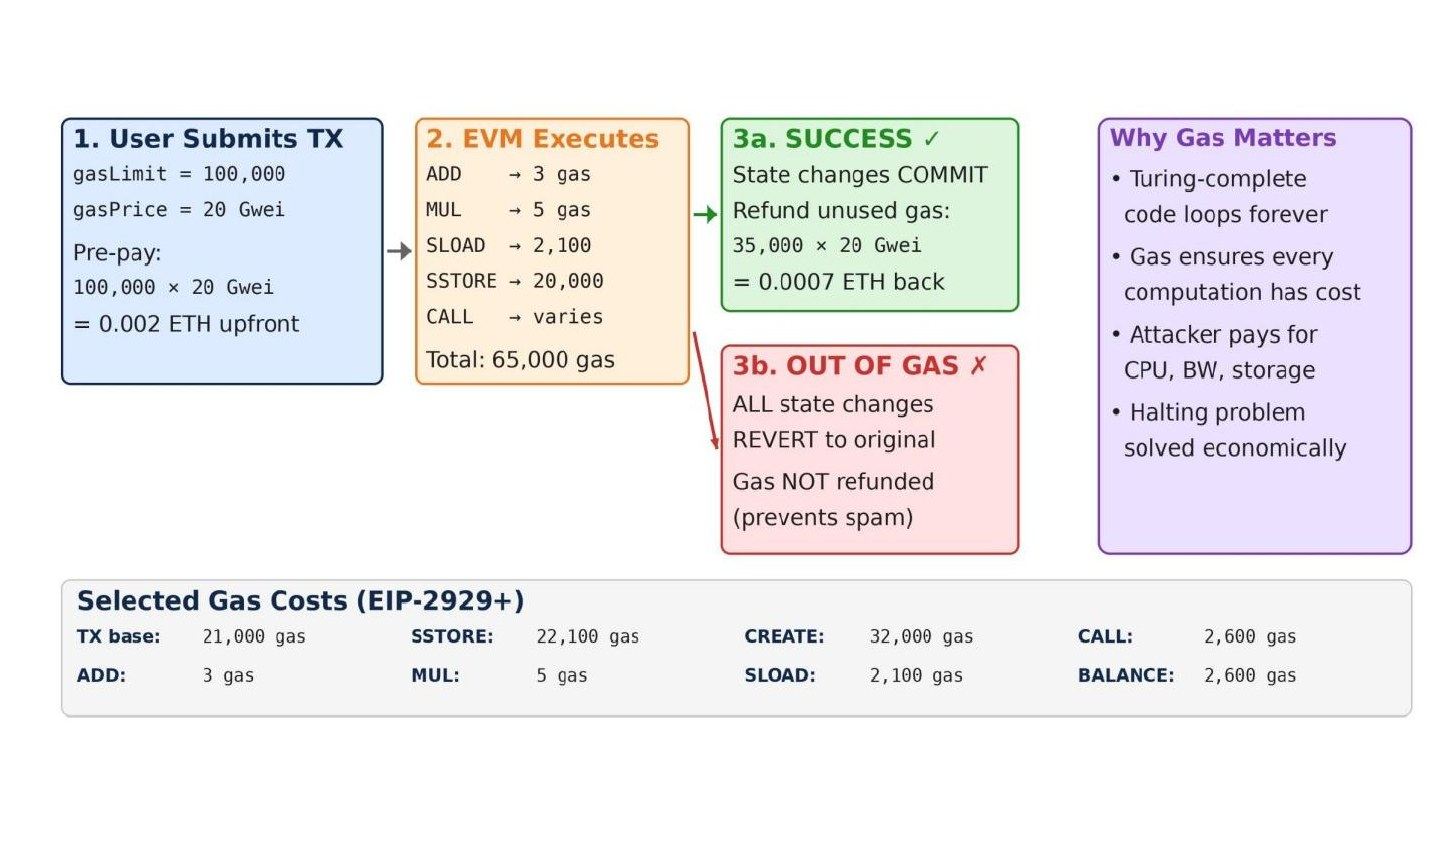
\includegraphics[keepaspectratio,alt={Diagramma riepilogativo del meccanismo del gas: flusso da TX submission a success/out-of-gas}]{images/lezione-19-ethereum-accounts-transactions-gas-img-13.jpg}}
\emph{Fig. --- Riepilogo del meccanismo gas. Il mittente specifica
gasLimit e gasPrice (es. 100.000 gas × 20 Gwei = 0.002 ETH upfront).
L'EVM esegue consumando gas. Se successo: gas non usato rimborsato. Se
out-of-gas: tutte le modifiche revertite, gas consumato NON rimborsato
(deterrente contro spam). In basso: tabella dei costi gas per le
istruzioni principali.}

\subsection{Costi delle operazioni
EVM}\label{costi-delle-operazioni-evm}

Il costo in gas di ogni istruzione è fisso e definito nel Yellow Paper
di Ethereum. Le operazioni di storage sono di gran lunga le più costose.

\pandocbounded{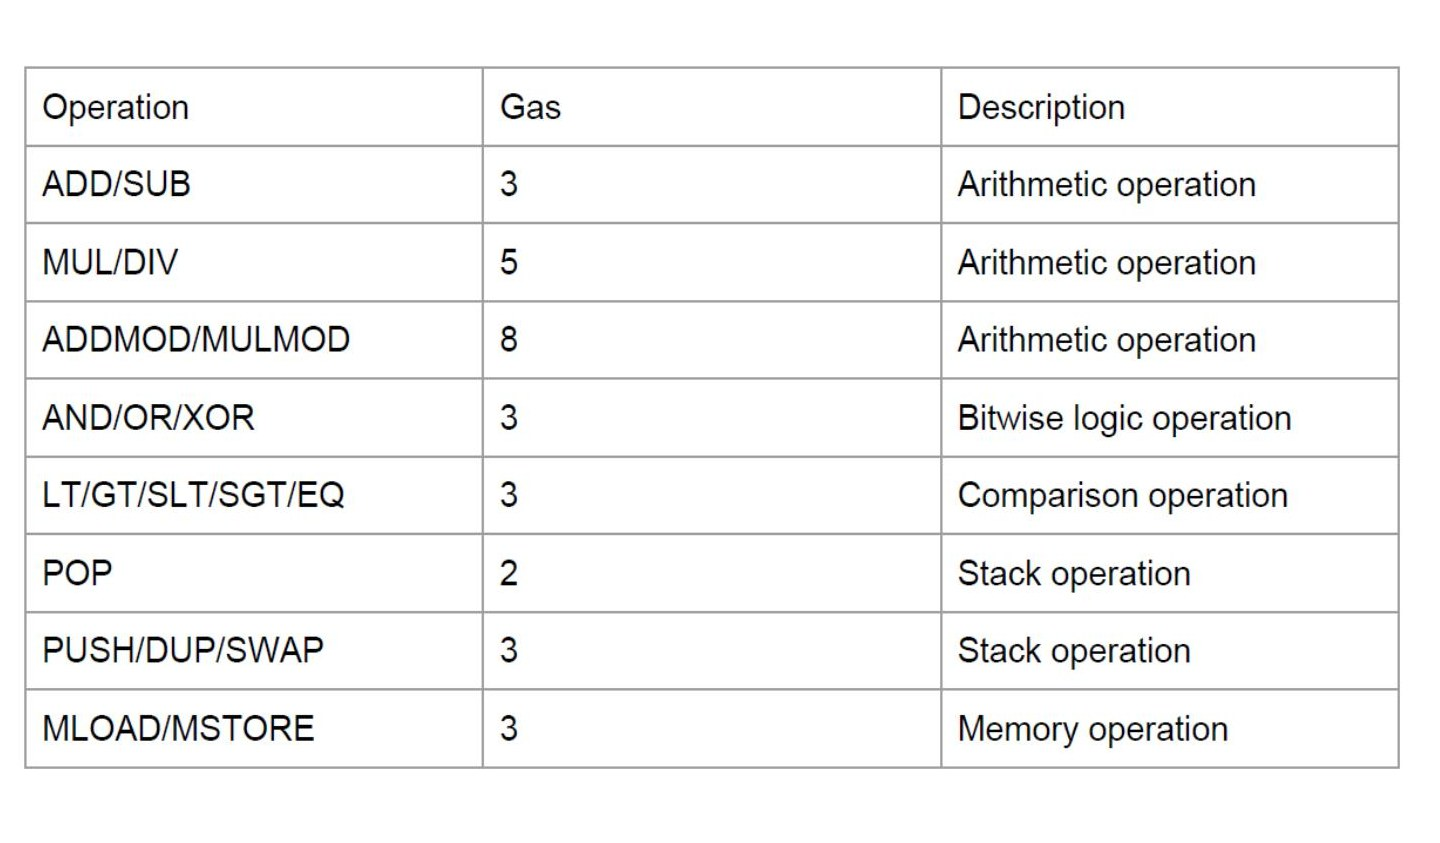
\includegraphics[keepaspectratio,alt={Tabella dei costi gas delle operazioni EVM di base}]{images/lezione-19-ethereum-accounts-transactions-gas-img-14.jpg}}
\emph{Fig. --- Costi gas per operazioni di base: ADD/SUB (3 gas),
MUL/DIV (5 gas), ADDMOD/MULMOD (8 gas), operazioni bitwise/confronto (3
gas), operazioni stack POP (2), PUSH/DUP/SWAP (3), MLOAD/MSTORE (3).}

\pandocbounded{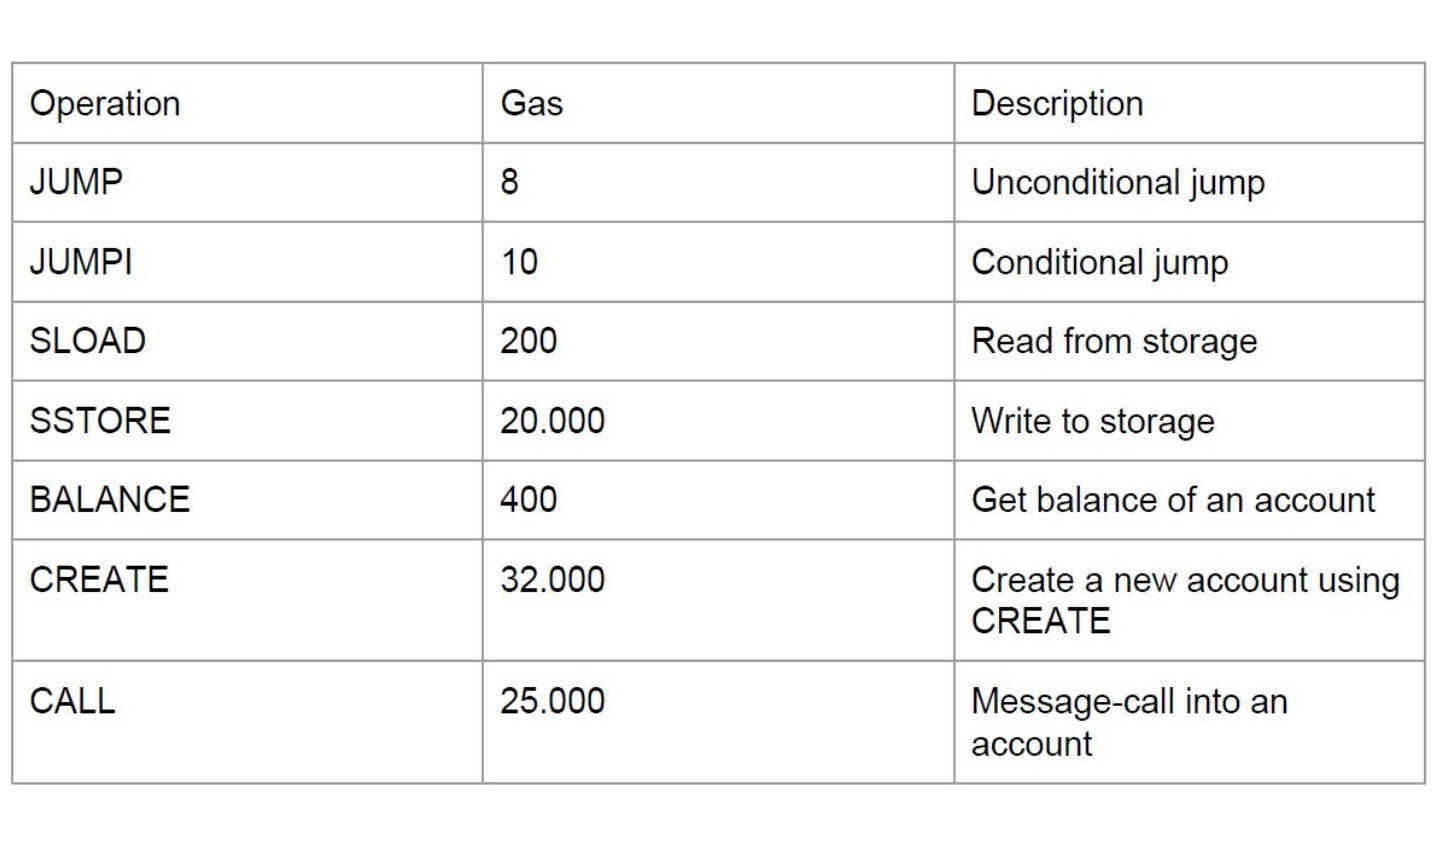
\includegraphics[keepaspectratio,alt={Tabella dei costi gas per operazioni avanzate: JUMP, storage, CREATE, CALL}]{images/lezione-19-ethereum-accounts-transactions-gas-img-15.jpg}}
\emph{Fig. --- Costi gas per operazioni avanzate: JUMP (8), JUMPI (10),
SLOAD (200), SSTORE (20.000), BALANCE (400), CREATE (32.000), CALL
(25.000). Lo storage è deliberatamente costoso per scoraggiare l'uso
eccessivo della chain come database.}

\subsection{Gas nei messaggi interni}\label{gas-nei-messaggi-interni}

I messaggi interni (da contratto a contratto) \textbf{non hanno un
proprio gas limit} separato: il gas limit dell'intera catena di
esecuzione è quello specificato nella transazione originale dell'EOA, e
deve essere sufficiente a coprire tutte le sub-esecuzioni. Se un
messaggio interno esaurisce il gas, quella specifica sub-esecuzione
viene revertita, ma la transazione padre può continuare se ha gestito il
caso d'errore.

\begin{center}\rule{0.5\linewidth}{0.5pt}\end{center}

\section{Ethereum e Bitcoin: confronto
finale}\label{ethereum-e-bitcoin-confronto-finale}

\pandocbounded{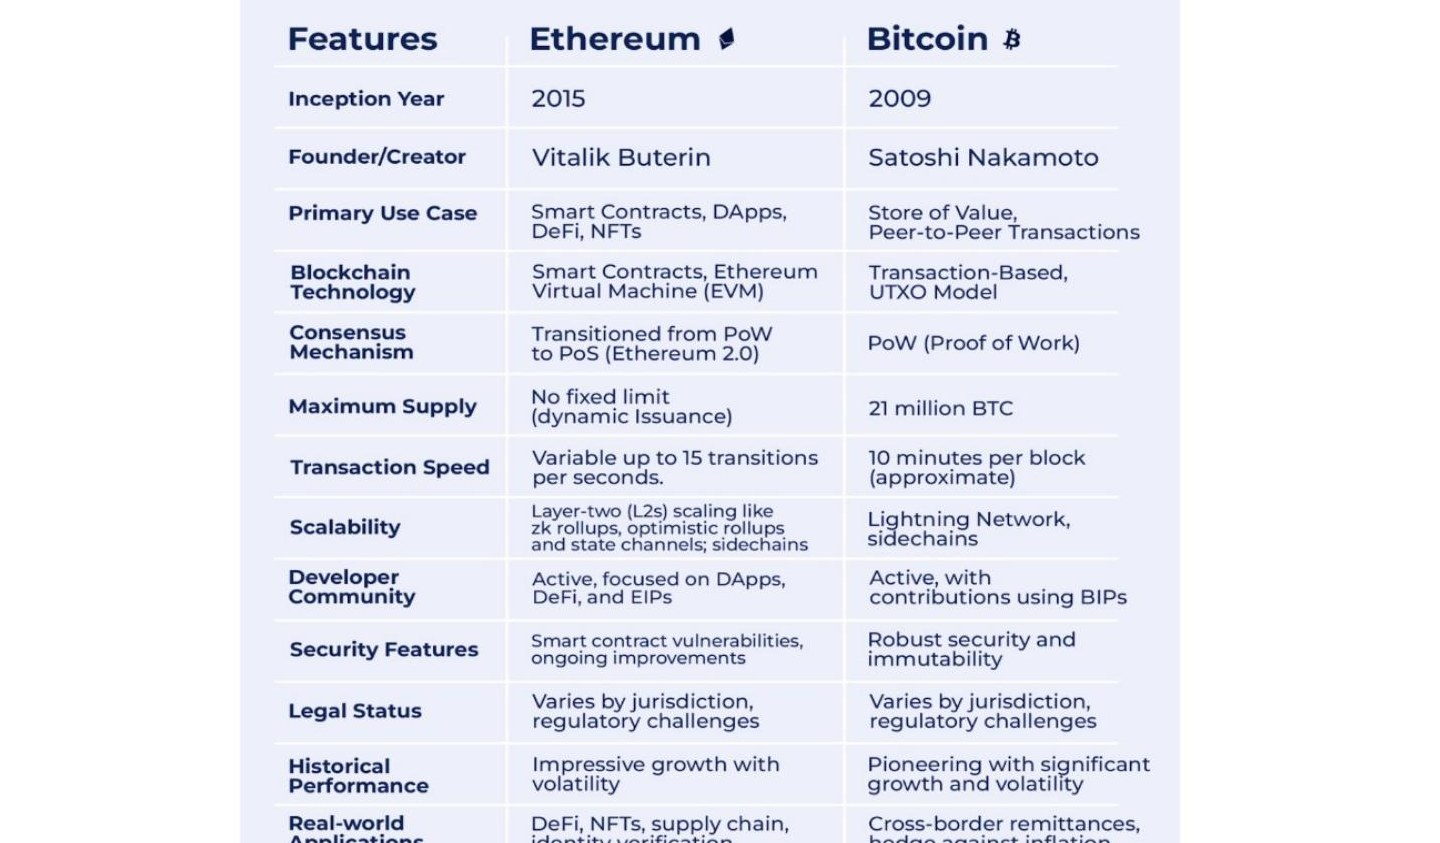
\includegraphics[keepaspectratio,alt={Tabella comparativa tra Ethereum e Bitcoin: caratteristiche principali}]{images/lezione-19-ethereum-accounts-transactions-gas-img-16.jpg}}
\emph{Fig. --- Confronto sistematico tra Ethereum (2015, Vitalik
Buterin) e Bitcoin (2009, Satoshi Nakamoto): use case, modello
blockchain, consenso, supply, velocità, sicurezza e community.}

{\def\LTcaptype{none} % do not increment counter
\begin{longtable}[]{@{}
  >{\raggedright\arraybackslash}p{(\linewidth - 4\tabcolsep) * \real{0.3214}}
  >{\raggedright\arraybackslash}p{(\linewidth - 4\tabcolsep) * \real{0.3571}}
  >{\raggedright\arraybackslash}p{(\linewidth - 4\tabcolsep) * \real{0.3214}}@{}}
\toprule\noalign{}
\begin{minipage}[b]{\linewidth}\raggedright
Feature
\end{minipage} & \begin{minipage}[b]{\linewidth}\raggedright
Ethereum
\end{minipage} & \begin{minipage}[b]{\linewidth}\raggedright
Bitcoin
\end{minipage} \\
\midrule\noalign{}
\endhead
\bottomrule\noalign{}
\endlastfoot
Inception & 2015 & 2009 \\
Fondatore & Vitalik Buterin & Satoshi Nakamoto \\
Use case principale & Smart Contracts, DApps, DeFi & Store of value, p2p
transactions \\
Tecnologia & Account-based, EVM & UTXO-based \\
Consenso & PoS (da settembre 2022) & PoW \\
Supply massima & Nessun limite fisso & 21 milioni di BTC \\
Linguaggio contratti & Solidity (Turing-completo) & Script (non
Turing-completo) \\
P2P layer & Kademlia & Protocollo proprietario \\
\end{longtable}
}

\begin{calloutnote}{Kademlia in Ethereum}

Ethereum usa {[}\hyperref[kademlia]{Kademlia}{]} come protocollo P2P per
la peer discovery, a differenza di Bitcoin che ha sviluppato il proprio
protocollo di gossip. Kademlia era già stato studiato nelle lezioni
precedenti come DHT efficiente.

\end{calloutnote}

\begin{center}\rule{0.5\linewidth}{0.5pt}\end{center}

\section{Cosa resta da discutere}\label{cosa-resta-da-discutere}

\begin{calloutnote}{Prossimi argomenti}

\begin{itemize}
\tightlist
\item
  \textbf{Programmazione degli smart contract}: Solidity (laboratorio)
\item
  \textbf{Struttura dei blocchi Ethereum}: log, Merkle Patricia Tries
\item
  \textbf{Proof of Stake}: meccanismo di consenso attuale
\item
  \textbf{Ethereum Virtual Machine (EVM)}: architettura e bytecode
\end{itemize}

\end{calloutnote}

\newpage

\chapter{Lezione 20 --- (Lab) Solidity}\label{lezione-20-lab-solidity}

\section{Ethereum: ripasso del modello degli
account}\label{ethereum-ripasso-del-modello-degli-account}

\subsection{Il modello account vs
UTXO}\label{il-modello-account-vs-utxo}

Ethereum adotta un \textbf{modello basato su account}, non su UTXO come
Bitcoin. Questo lo rende concettualmente più simile a un conto bancario:
ogni account ha un saldo che può essere incrementato o decrementato
direttamente, il ``cambio'' è implicito, e la verifica della firma è
fatta sull'account stesso (non su script).

L'identificatore di un account è gli ultimi 160 bit dell'hash
\textbf{Keccak-256} della chiave pubblica --- non c'è un encoding
human-friendly come in Bitcoin (no Base58Check).

\subsection{EOA vs Contract account}\label{eoa-vs-contract-account}

Esistono due tipi di account:

\begin{itemize}
\tightlist
\item
  \textbf{EOA} (\emph{Externally Owned Account}): account controllato da
  una chiave privata, l'unico che può \emph{iniziare} transazioni
  autonomamente.
\item
  \textbf{Contract}: account senza chiave privata, il cui comportamento
  è determinato da bytecode EVM. Viene attivato solo quando riceve una
  transazione.
\end{itemize}

\pandocbounded{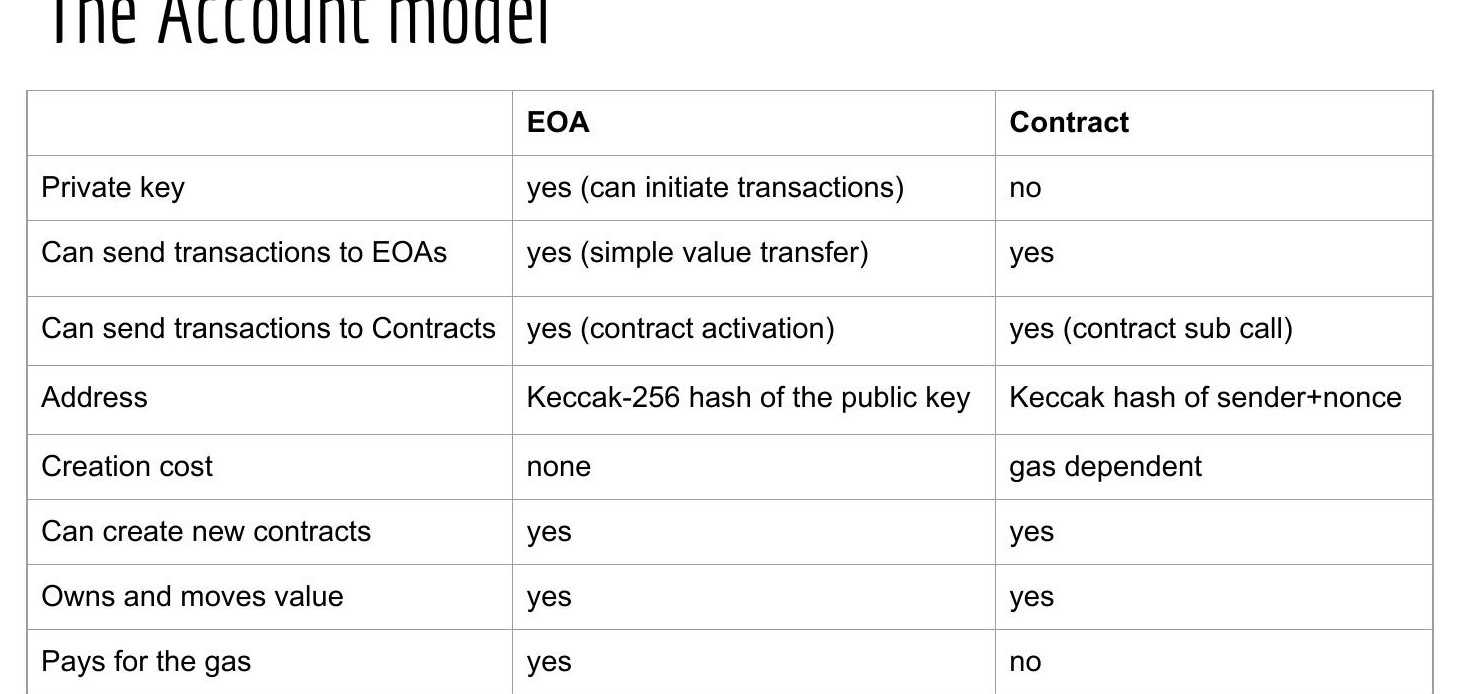
\includegraphics[keepaspectratio,alt={Tabella comparativa EOA vs Contract account in Ethereum}]{images/lezione-20-lab-solidity-img-01.jpg}}
\emph{Fig. --- Confronto tra EOA e Contract: solo l'EOA possiede una
chiave privata e paga il gas. Il Contract riceve il proprio indirizzo
come hash di sender+nonce alla creazione.}

\subsection{Campi di ogni account}\label{campi-di-ogni-account}

Tutti gli account, sia EOA che Contract, condividono quattro campi:

\begin{itemize}
\tightlist
\item
  \textbf{nonce} --- numero di transazioni inviate dall'account (per
  EOA) o numero di contratti creati (per Contract, da 1). Previene la
  \emph{malleability} e garantisce l'ordinamento: campo
  \textbf{dinamico}.
\item
  \textbf{balance} --- quantità di wei posseduti, espressa come intero:
  \textbf{dinamico}.
\item
  \textbf{codeHash} --- hash del bytecode EVM del contratto (per gli EOA
  è l'hash della stringa vuota). Il codice vero e proprio è conservato
  nel database di stato sotto il suo hash: \textbf{statico}.
\item
  \textbf{storageRoot} --- hash della radice di un \emph{Merkle Patricia
  Trie} che codifica lo storage dell'account (una mappa da interi a
  interi), vuoto per default: \textbf{dinamico}.
\end{itemize}

\begin{callouttip}{Statico vs Dinamico}

\texttt{codeHash} è l'unico campo \textbf{statico}: il bytecode di un
contratto non cambia dopo il deployment. Tutti gli altri campi variano
ad ogni transazione che li coinvolge.

\end{callouttip}

\begin{center}\rule{0.5\linewidth}{0.5pt}\end{center}

\section{Lo stato di Ethereum}\label{lo-stato-di-ethereum}

Lo stato globale di Ethereum è strutturato come una gerarchia di
\textbf{Merkle Patricia Trie}. Ogni blocco contiene nel suo header tre
radici di trie:

\begin{itemize}
\tightlist
\item
  \textbf{stateRoot} --- la radice del World State Trie, che mappa ogni
  indirizzo ai quattro campi dell'account.
\item
  \textbf{transactionsRoot} --- la radice del Transactions Trie, dove la
  chiave è l'indice della transazione nel blocco (da 0).
\item
  \textbf{receiptsRoot} --- la radice del Receipts Trie, che contiene i
  risultati dell'esecuzione di ogni transazione.
\end{itemize}

\pandocbounded{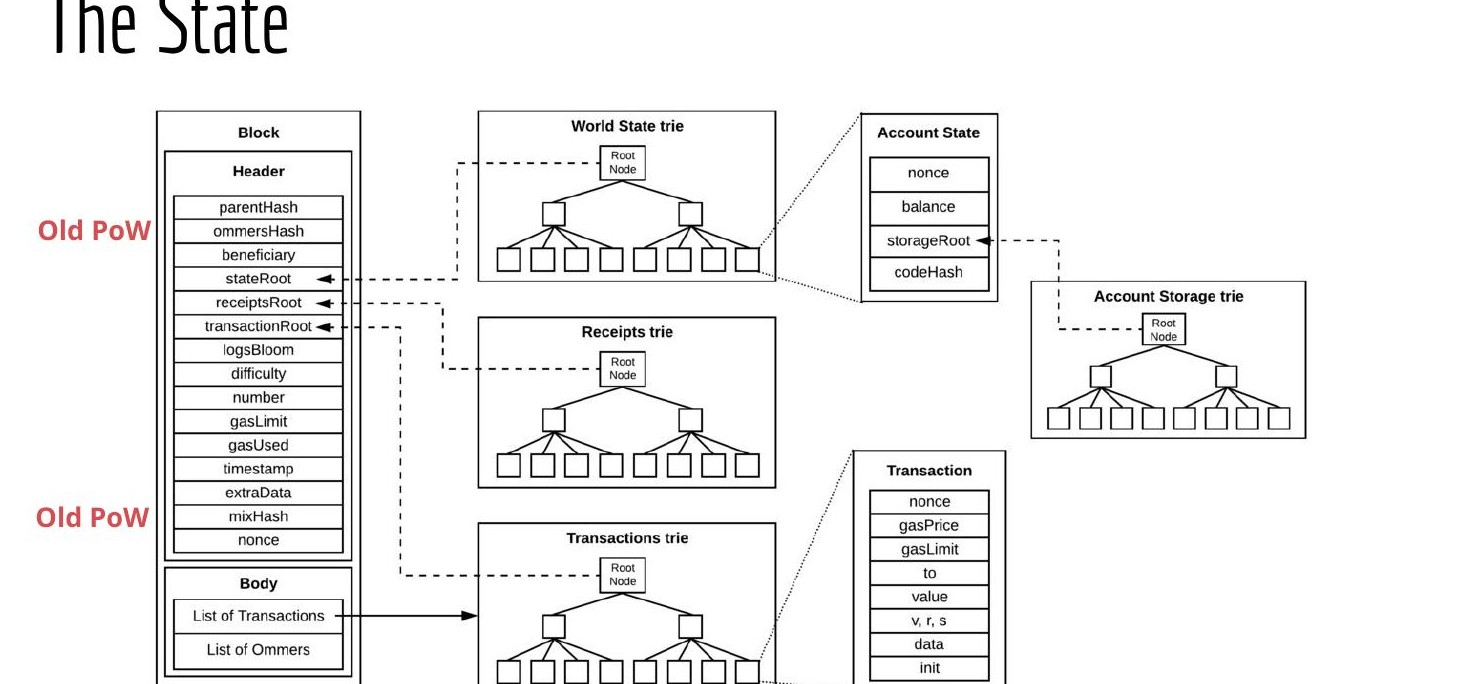
\includegraphics[keepaspectratio,alt={Struttura del World State Trie con Account State e Account Storage Trie collegati al Block Header}]{images/lezione-20-lab-solidity-img-02.jpg}}
\emph{Fig. --- Il block header punta via hash a tre trie: World State,
Receipts e Transactions. L'Account State contiene nonce, balance,
storageRoot e codeHash; lo storageRoot punta a sua volta all'Account
Storage Trie.}

La struttura si replica su blocchi successivi: ogni nuovo blocco N+1
condivide i nodi immutati con il blocco N (persistent data structure) e
crea nuovi nodi solo per gli account modificati.

\pandocbounded{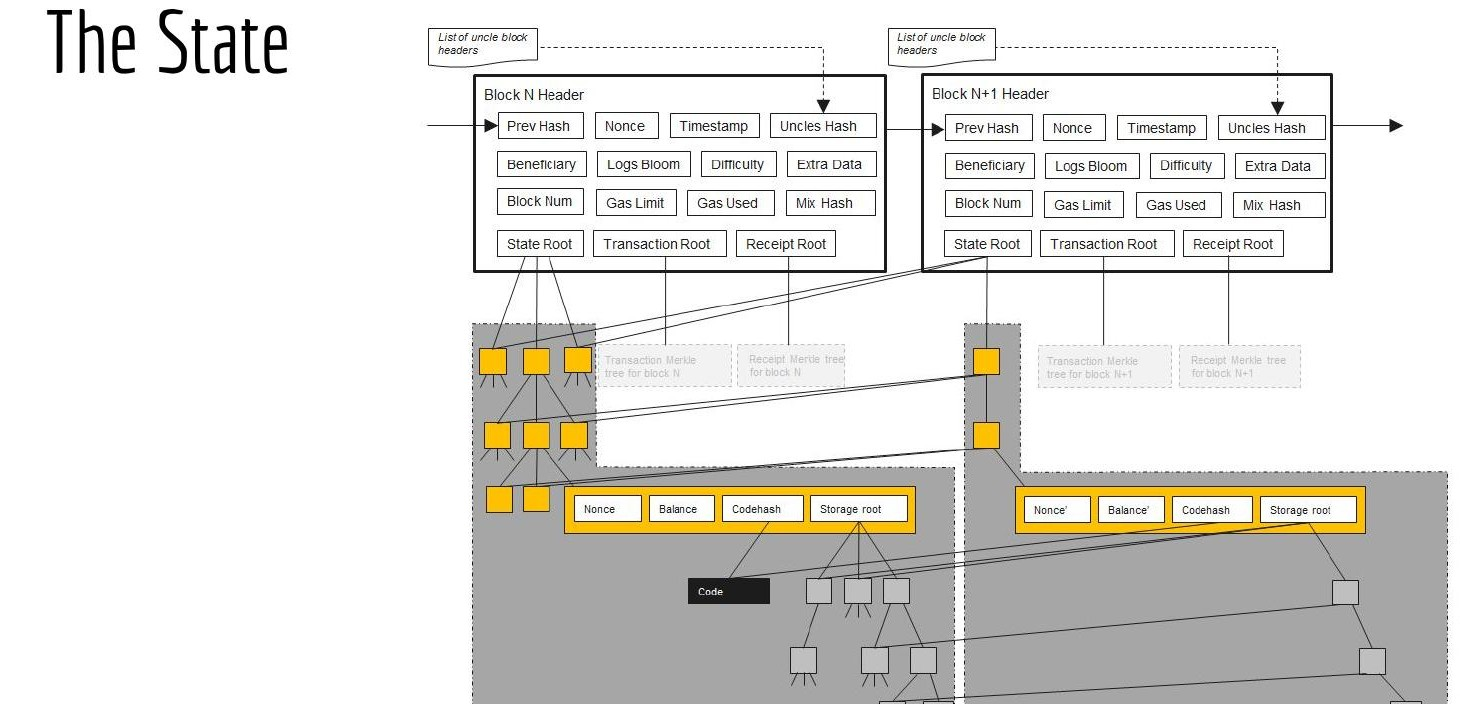
\includegraphics[keepaspectratio,alt={Struttura completa di due blocchi consecutivi con State, Transaction e Receipt Trie condivisi}]{images/lezione-20-lab-solidity-img-03.jpg}}
\emph{Fig. --- I blocchi N e N+1 mostrano come i Merkle Patricia Trie si
propaghino tra blocchi: le foglie gialle rappresentano gli account
modificati, i nodi condivisi rimangono inalterati.}

\subsection{Receipt e Bloom filter}\label{receipt-e-bloom-filter}

Per ogni transazione viene generata una \textbf{receipt} contenente:

\begin{itemize}
\tightlist
\item
  \texttt{medstate} --- root del state trie dopo l'elaborazione della
  transazione.
\item
  \texttt{gas\_used} --- gas consumato cumulativo dopo la transazione.
\item
  \texttt{logs} --- lista di voci della forma
  \texttt{{[}address,\ {[}topic1,\ topic2...{]},\ data{]}}, generate
  dagli opcode \texttt{LOG0}\ldots{}\texttt{LOG4} durante l'esecuzione
  (incluse le sub-call). L'indirizzo è quello del contratto che ha
  emesso il log, i topic sono fino a 4 valori da 32 byte.
\item
  \texttt{logBloom} --- \textbf{Bloom filter} costruito su indirizzi e
  topic di tutti i log della transazione.
\end{itemize}

L'OR bit a bit di tutti i \texttt{logBloom} delle receipt viene inserito
nell'header del blocco. Questo permette a client leggeri di verificare
rapidamente se un blocco contiene log rilevanti senza scaricare l'intero
stato.

\begin{calloutdefinition}{Bloom filter}

Struttura dati probabilistica che permette di verificare l'appartenenza
di un elemento a un insieme in tempo costante. Può restituire falsi
positivi ma mai falsi negativi. Nel contesto Ethereum, consente di
filtrare efficientemente i blocchi rilevanti per una query su eventi.

\end{calloutdefinition}

\subsection{Log ed eventi in Solidity}\label{log-ed-eventi-in-solidity}

I log risiedono \textbf{sopra} lo stato EVM interno e non sono visibili
ai contratti durante l'esecuzione. Sono pensati per applicazioni
esterne, che possono sottoscriversi a specifici tipi di log senza dover
rieseguire tutte le transazioni o mantenere lo stato.

In Solidity i log si usano tramite gli \textbf{eventi}:

\begin{Shaded}
\begin{Highlighting}[]
\NormalTok{event moneySent(address indexed \_from, address \_to, uint \_amount);}

\NormalTok{function sendMoney(address \_to, uint \_amount) public returns (bool) \{}
\NormalTok{    require(Balance[msg.sender] \textgreater{}= \_amount, "Not enough value");}
\NormalTok{    moneyBalance[msg.sender] {-}= \_amount;}
\NormalTok{    moneyBalance[\_to] += \_amount;}
\NormalTok{    emit moneySent(msg.sender, \_to, \_amount);}
\NormalTok{    return true;}
\NormalTok{\}}
\end{Highlighting}
\end{Shaded}

Il parametro \texttt{indexed} su \texttt{\_from} significa che il topic
corrispondente viene incluso nel Bloom filter, rendendo le query per
mittente molto efficienti.

\begin{calloutnote}{Smart contract e source code}

Nello stato EVM è conservato solo il \textbf{bytecode} compilato, non il
sorgente Solidity. I sorgenti visibili su explorer come Etherscan sono
caricati volontariamente dagli sviluppatori e verificati dall'explorer
tramite compilazione.

\end{calloutnote}

\begin{center}\rule{0.5\linewidth}{0.5pt}\end{center}

\section{Gas}\label{gas}

Il \textbf{gas} è il meccanismo che risolve due problemi fondamentali
dell'EVM, resa Turing-completa dagli smart contract:

\begin{enumerate}
\def\labelenumi{\arabic{enumi}.}
\tightlist
\item
  \textbf{Anti-DDoS}: senza un costo per l'esecuzione, un attaccante
  potrebbe inviare transazioni con loop infiniti bloccando la rete.
\item
  \textbf{Utilizzo equo delle risorse}: ogni operazione ha un costo in
  gas proporzionale al lavoro computazionale richiesto.
\end{enumerate}

Il gas viene pagato per l'\textbf{esecuzione} (opcode EVM) e per lo
\textbf{storage} (scrittura nello stato). Aspetto importante: il gas
viene pagato anche per transazioni che falliscono o che esauriscono il
gas --- il lavoro già fatto deve essere compensato.

\begin{calloutwarning}{gaslimit a livello di transazione}

Il mittente specifica un \texttt{gaslimit} nella transazione: se il
contratto consuma più gas del limite, l'esecuzione si interrompe con un
\textbf{revert} (lo stato viene ripristinato) ma il gas già consumato
viene comunque pagato. Questo protegge da comportamenti inattesi,
incluse sub-call a contratti esterni.

\end{calloutwarning}

Il \texttt{gaslimit} a livello di blocco (analogo alla block size di
Bitcoin) limita il tempo di validazione di un blocco e quindi la
quantità di computazione per blocco.

I costi in gas per operazione sono \textbf{hardcodati} nell'Appendice G
del Yellow Paper di Ethereum. Esiste inoltre un insieme speciale di
indirizzi (da \texttt{0x01} a \texttt{0x0a}) che contengono
\textbf{precompiled contracts}: contratti il cui comportamento non è
definito da bytecode EVM ma è implementato direttamente nell'esecuzione
environment (Appendice E del Yellow Paper). Si chiamano come contratti
normali ma il loro gas consumption è anch'esso predefinito.

\begin{center}\rule{0.5\linewidth}{0.5pt}\end{center}

\section{Solidity}\label{solidity}

\textbf{Solidity} è il linguaggio di programmazione ad alto livello per
smart contract su Ethereum. Si compila in bytecode EVM.

Caratteristiche principali: - \textbf{Staticamente tipato}: i tipi
vengono verificati a tempo di compilazione. - \textbf{Object Oriented}:
un contratto si modella come un'istanza di classe, con stato (variabili
di stato) e metodi (funzioni). - \textbf{In continuo sviluppo}: la
documentazione ufficiale è su
\texttt{https://docs.soliditylang.org/en/latest/}.

\subsection{Remix IDE}\label{remix-ide}

Lo strumento standard per sviluppare e testare contratti Solidity è
\textbf{Remix IDE}, accessibile via browser.

\pandocbounded{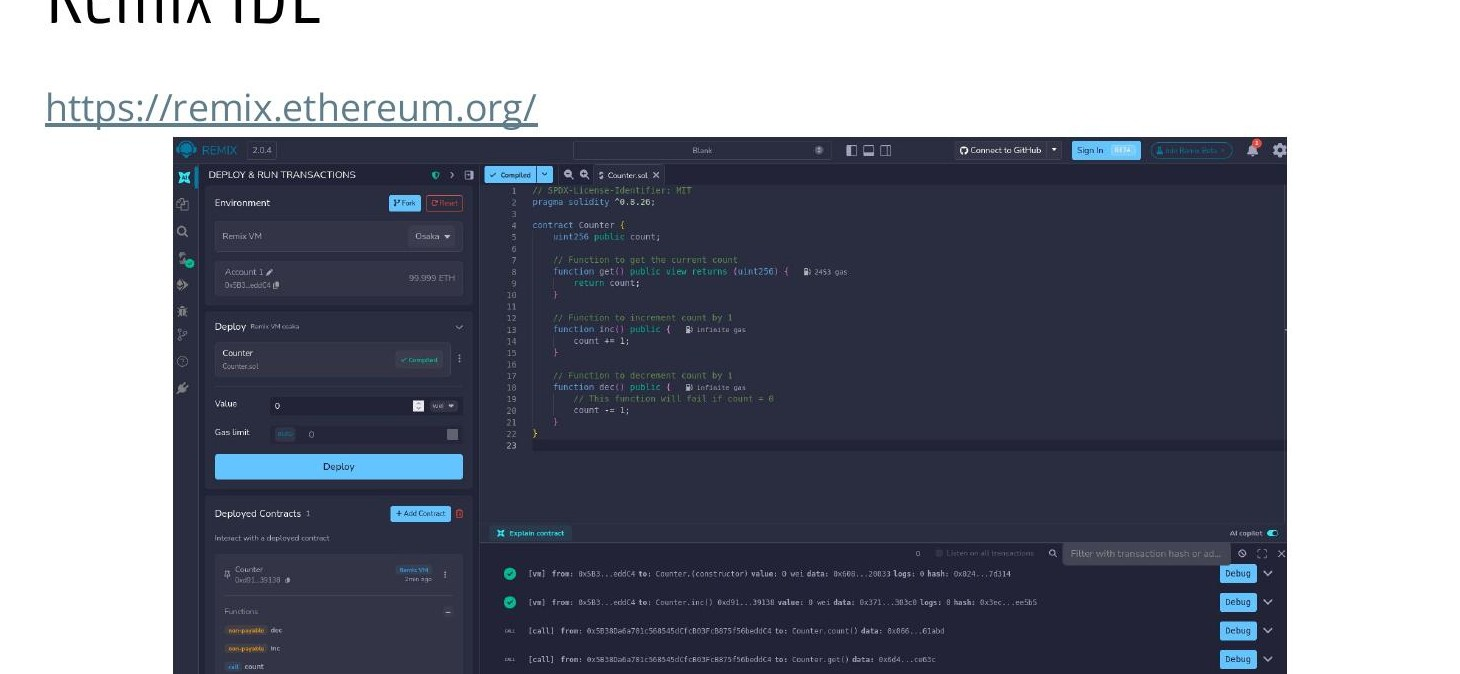
\includegraphics[keepaspectratio,alt={Screenshot di Remix IDE con il contratto Counter deployato e i log delle transazioni}]{images/lezione-20-lab-solidity-img-04.jpg}}
\emph{Fig. --- Remix IDE: pannello di deploy a sinistra, editor con
Counter.sol al centro, log delle transazioni in basso. Si vedono le
chiamate a \texttt{inc}, \texttt{dec}, \texttt{get} con i rispettivi
hash e gas usato.}

\subsection{Primo contratto: Counter}\label{primo-contratto-counter}

Il contratto \texttt{Counter} è l'esempio introduttivo classico. Il
workflow su Remix:

\begin{enumerate}
\def\labelenumi{\arabic{enumi}.}
\tightlist
\item
  Creare un nuovo file \texttt{Counter.sol}
\item
  Copiare il codice
\item
  Compilare
\item
  Deploy su VM (ambiente locale simulato)
\item
  Chiamare i metodi
\item
  Ispezionare le receipt delle transazioni
\end{enumerate}

\pandocbounded{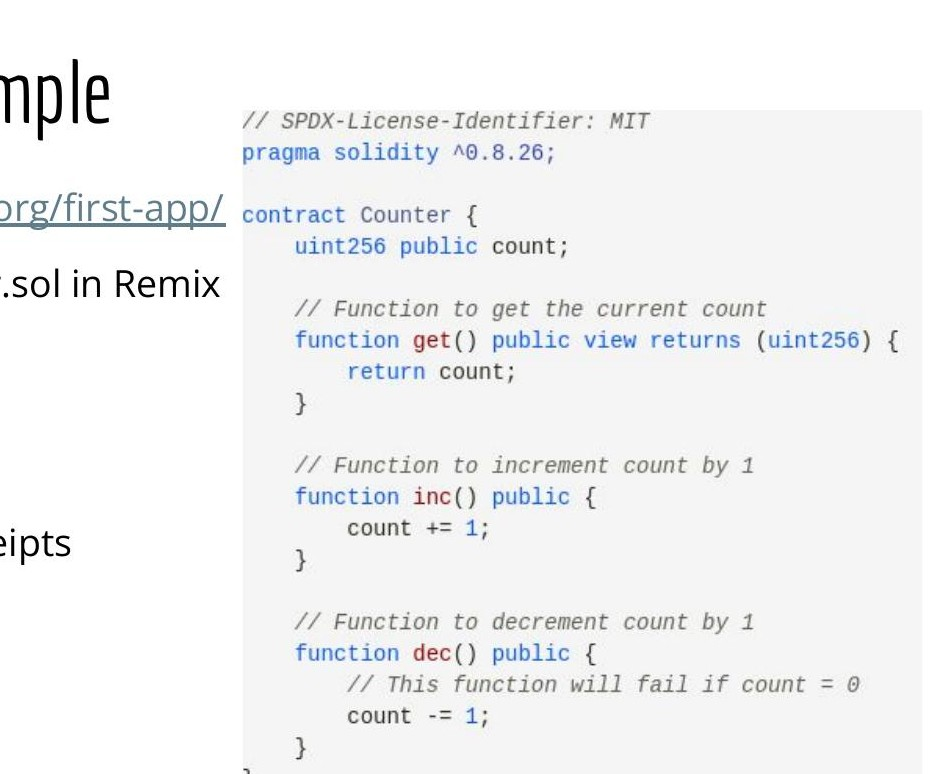
\includegraphics[keepaspectratio,alt={Codice del contratto Counter.sol in Solidity}]{images/lezione-20-lab-solidity-img-05.jpg}}
\emph{Fig. --- Il contratto Counter: variabile di stato
\texttt{uint256\ public\ count}, funzioni \texttt{get()} (view),
\texttt{inc()} e \texttt{dec()} (public). La funzione \texttt{dec()}
fallisce se \texttt{count\ =\ 0} per underflow aritmetico.}

\subsection{Pragma e versioning}\label{pragma-e-versioning}

La direttiva \texttt{pragma} specifica la versione del compilatore
Solidity richiesta. La semantica del versioning segue regole precise:

{\def\LTcaptype{none} % do not increment counter
\begin{longtable}[]{@{}
  >{\raggedright\arraybackslash}p{(\linewidth - 2\tabcolsep) * \real{0.5000}}
  >{\raggedright\arraybackslash}p{(\linewidth - 2\tabcolsep) * \real{0.5000}}@{}}
\toprule\noalign{}
\begin{minipage}[b]{\linewidth}\raggedright
Direttiva
\end{minipage} & \begin{minipage}[b]{\linewidth}\raggedright
Significato
\end{minipage} \\
\midrule\noalign{}
\endhead
\bottomrule\noalign{}
\endlastfoot
\texttt{pragma\ solidity\ 0.4.16} & Esattamente la versione 0.4.16 \\
\texttt{pragma\ solidity\ \textgreater{}=0.4.16\ \textless{}0.7.1} &
Dalla 0.4.16 (inclusa) alla 0.7.1 (esclusa) \\
\texttt{pragma\ solidity\ \^{}0.4.16} & Dalla 0.4.16 alla 0.5.0
(esclusa) \\
\end{longtable}
}

La versione \texttt{x.y.*} introduce breaking change rispetto a
\texttt{x-1.*.*} o \texttt{x.y-1.*}.

\subsection{Import}\label{import}

Solidity supporta diversi meccanismi di import per la modularizzazione
del codice:

\begin{Shaded}
\begin{Highlighting}[]
\NormalTok{import "lib/util.sol";                        // import diretto}
\NormalTok{import "../token.sol";                         // import relativo}
\NormalTok{import * as tokenLibrary from "lib/token.sol"; // rinomina namespace}
\NormalTok{// uso: tokenLibrary.varName1}
\end{Highlighting}
\end{Shaded}

\subsection{Costrutti principali}\label{costrutti-principali}

Un contratto Solidity è composto da quattro categorie di costrutti:

\begin{itemize}
\tightlist
\item
  \textbf{State Variables} --- variabili persistenti nello storage del
  contratto.
\item
  \textbf{Functions} --- le operazioni che il contratto espone o usa
  internamente.
\item
  \textbf{Errors e Modifiers} --- meccanismi di validazione e pattern
  guard.
\item
  \textbf{Events} --- log emessi durante l'esecuzione, visibili alle
  applicazioni esterne.
\end{itemize}

\subsection{Visibility Modifiers}\label{visibility-modifiers}

La visibilità controlla chi può accedere a variabili e funzioni.

\textbf{Variabili di stato:}

{\def\LTcaptype{none} % do not increment counter
\begin{longtable}[]{@{}
  >{\raggedright\arraybackslash}p{(\linewidth - 2\tabcolsep) * \real{0.5000}}
  >{\raggedright\arraybackslash}p{(\linewidth - 2\tabcolsep) * \real{0.5000}}@{}}
\toprule\noalign{}
\begin{minipage}[b]{\linewidth}\raggedright
Modificatore
\end{minipage} & \begin{minipage}[b]{\linewidth}\raggedright
Comportamento
\end{minipage} \\
\midrule\noalign{}
\endhead
\bottomrule\noalign{}
\endlastfoot
\texttt{public} & Visibile internamente + getter automatico con
visibilità esterna (\texttt{view}) \\
\texttt{internal} & \emph{Default.} Visibile nel contratto e nei
contratti derivati \\
\texttt{private} & Solo nel contratto corrente, non nei derivati \\
\end{longtable}
}

\textbf{Funzioni:}

{\def\LTcaptype{none} % do not increment counter
\begin{longtable}[]{@{}
  >{\raggedright\arraybackslash}p{(\linewidth - 2\tabcolsep) * \real{0.5000}}
  >{\raggedright\arraybackslash}p{(\linewidth - 2\tabcolsep) * \real{0.5000}}@{}}
\toprule\noalign{}
\begin{minipage}[b]{\linewidth}\raggedright
Modificatore
\end{minipage} & \begin{minipage}[b]{\linewidth}\raggedright
Comportamento
\end{minipage} \\
\midrule\noalign{}
\endhead
\bottomrule\noalign{}
\endlastfoot
\texttt{external} & Chiamabile solo da transazioni/messaggi esterni
(internamente via \texttt{this.fun()}) \\
\texttt{public} & Chiamabile sia da esterno che internamente \\
\texttt{internal} & Solo dal contratto corrente o derivati --- non fa
parte dell'ABI \\
\texttt{private} & Solo dal contratto corrente --- non fa parte
dell'ABI \\
\end{longtable}
}

\begin{calloutwarning}{private non significa segreto}

Una variabile \texttt{private} non è accessibile via chiamate Solidity,
ma il suo valore è comunque leggibile direttamente dallo storage
on-chain da chiunque. In Ethereum non esiste vera riservatezza dei dati
in-chain.

\end{calloutwarning}

\begin{callouttip}{ABI e visibilità esterna}

L'\textbf{ABI} (\emph{Application Binary Interface}) è l'interfaccia
pubblica del contratto: descrive le funzioni e gli eventi visibili
dall'esterno. Solo le funzioni \texttt{external} e \texttt{public} fanno
parte dell'ABI e possono essere chiamate da transazioni o da altri
contratti tramite call standard.

\end{callouttip}

\newpage

\chapter{Lab 7 --- Solidity (avanzato)}\label{lab-7-solidity-avanzato}

Questa lezione prosegue l'introduzione a Solidity approfondendo il
sistema dei tipi, le funzioni, la gestione degli errori, i modifier e
gli eventi. Si tratta del cuore del linguaggio: capire come Solidity
gestisce i tipi, la mutabilità dello stato e il controllo degli accessi
è fondamentale per scrivere contratti corretti e sicuri.

\begin{center}\rule{0.5\linewidth}{0.5pt}\end{center}

\section{Solidity: ripasso rapido}\label{solidity-ripasso-rapido}

Solidity è un linguaggio \textbf{staticamente tipato},
\textbf{object-oriented}, compilato in bytecode EVM. Un contratto è
modellato come una classe con stato (variabili di storage persistenti) e
metodi (funzioni). La documentazione ufficiale è su
\texttt{https://docs.soliditylang.org/en/latest/}.

Il primo contratto di riferimento è \texttt{Counter.sol}, da deployare
su Remix IDE:

\pandocbounded{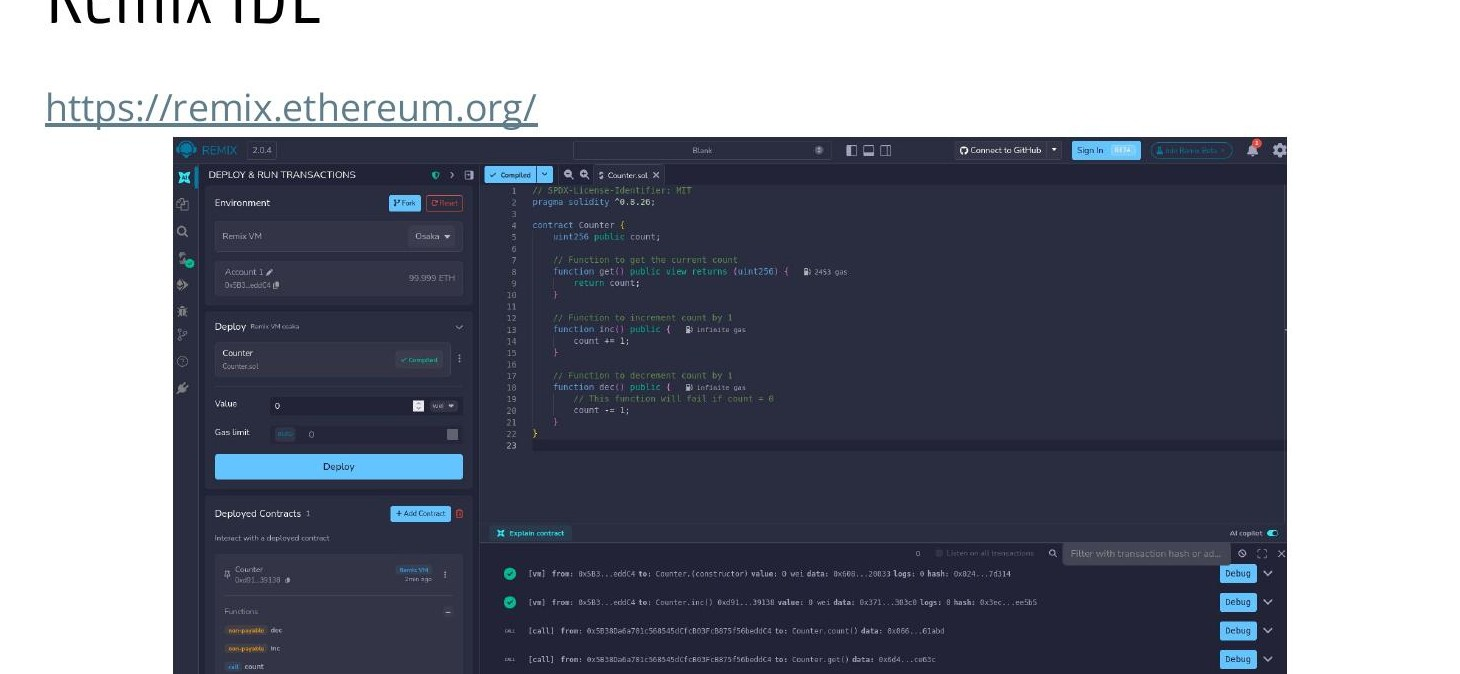
\includegraphics[keepaspectratio,alt={Screenshot di Remix IDE con Counter.sol deployato e log delle transazioni}]{images/lezione-21-lab-solidity-avanzato-img-01.jpg}}
\emph{Fig. --- Remix IDE: a sinistra il pannello di deploy, al centro
l'editor con Counter.sol, in basso i log delle transazioni con hash, gas
usato e valori restituiti.}

\pandocbounded{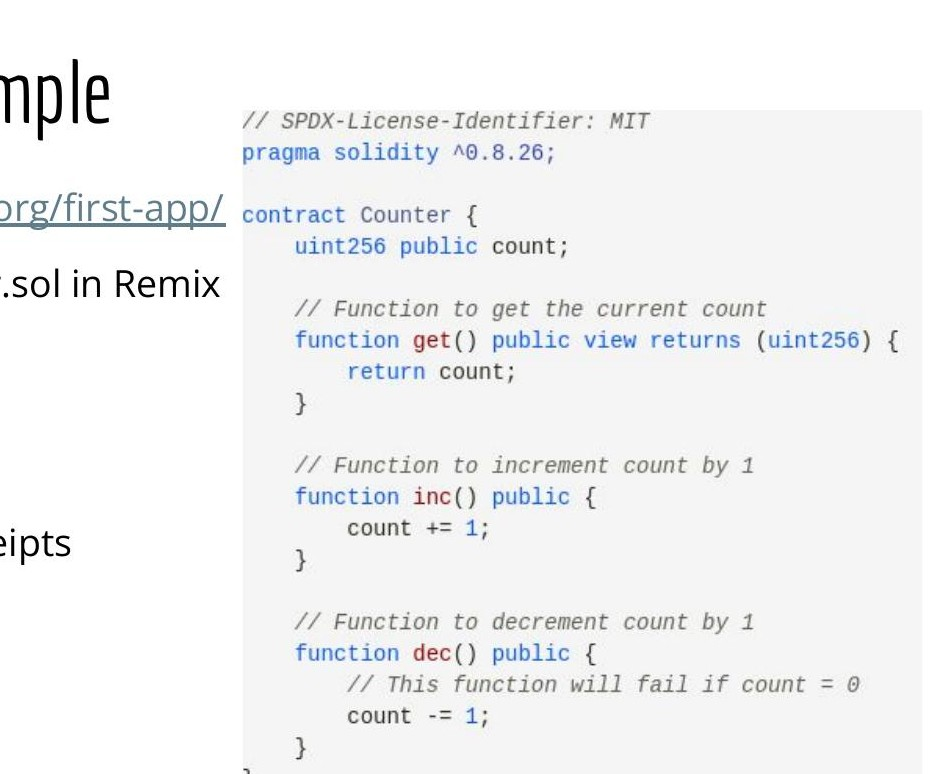
\includegraphics[keepaspectratio,alt={Codice sorgente del contratto Counter.sol}]{images/lezione-21-lab-solidity-avanzato-img-02.jpg}}
\emph{Fig. --- Counter.sol: variabile di stato
\texttt{uint256\ public\ count}, funzione \texttt{get()} con
modificatore \texttt{view}, \texttt{inc()} e \texttt{dec()} pubbliche.
La \texttt{dec()} fallisce per underflow se \texttt{count\ ==\ 0}.}

\begin{center}\rule{0.5\linewidth}{0.5pt}\end{center}

\section{Il sistema dei tipi}\label{il-sistema-dei-tipi}

Solidity distingue due grandi famiglie di tipi: \textbf{value types} e
\textbf{reference types}. La dichiarazione segue la sintassi
\texttt{tipo\ {[}modificatore{]}\ nome;}.

I \textbf{value types} non specificano un'area di memoria (il
compilatore li colloca nello stack se efimeri, nello storage se
variabili di stato). Possono avere qualificatori: - \texttt{transient}
--- come lo storage ma valido solo per la durata di una singola
transazione. - \texttt{constant} --- valore sostituito a tempo di
compilazione. - \texttt{immutable} --- valore fissato a tempo di
costruzione del contratto.

I \textbf{reference types} devono specificare esplicitamente l'area di
memoria: \texttt{memory} (temporanea, per la durata della chiamata),
\texttt{storage} (persistente, nel trie dell'account), o
\texttt{calldata} (read-only, per i parametri di funzioni
\texttt{external}).

\subsection{Value Types}\label{value-types}

\textbf{Booleano e interi:}

\begin{Shaded}
\begin{Highlighting}[]
\NormalTok{bool flag;                  // true / false}
\NormalTok{int8 .. int256              // interi con segno (int == int256)}
\NormalTok{uint8 .. uint256            // interi senza segno (uint == uint256)}
\end{Highlighting}
\end{Shaded}

Le divisioni intere arrotondano sempre verso zero (troncamento). I
numeri in virgola mobile esistono (\texttt{fixed}/\texttt{ufixed}) ma
sono molto limitati nella versione attuale.

\textbf{Byte e stringhe:}

\begin{Shaded}
\begin{Highlighting}[]
\NormalTok{bytes1, bytes2, ..., bytes32    // array di byte a dimensione fissa}
\NormalTok{string                          // sequenza di caratteri UTF{-}8}
\end{Highlighting}
\end{Shaded}

\textbf{Enum:} tipo enumerato con al massimo 256 membri. Internamente
rappresentato come \texttt{uint8}. Quando esposto all'ABI esterna, la
firma viene tradotta automaticamente in \texttt{uint8}.

\begin{Shaded}
\begin{Highlighting}[]
\NormalTok{contract test \{}
\NormalTok{    enum ActionChoices \{ GoLeft, GoRight, GoStraight, SitStill \}}
\NormalTok{    ActionChoices choice;}
\NormalTok{    ActionChoices constant defaultChoice = ActionChoices.GoStraight;}

\NormalTok{    function setGoStraight() public \{}
\NormalTok{        choice = ActionChoices.GoStraight;}
\NormalTok{    \}}
\NormalTok{    // Per l\textquotesingle{}ABI esterna getChoice() diventa "getChoice() returns (uint8)"}
\NormalTok{    function getChoice() public view returns (ActionChoices) \{}
\NormalTok{        return choice;}
\NormalTok{    \}}
\NormalTok{\}}
\end{Highlighting}
\end{Shaded}

\subsection{\texorpdfstring{Il tipo
\texttt{address}}{Il tipo address}}\label{il-tipo-address}

Il tipo \texttt{address} è fondamentale in Solidity: rappresenta un
indirizzo Ethereum a 20 byte. Esistono due varianti:

\begin{itemize}
\tightlist
\item
  \texttt{address} --- solo lettura.
\item
  \texttt{address\ payable} --- può ricevere Ether (convertibile da
  \texttt{address} con \texttt{payable(...)}).
\end{itemize}

Gli indirizzi hex che superano il checksum EIP-55 sono letterali di tipo
\texttt{address} (es.
\texttt{0xdCad3a6d3569DF655070DEd06cb7A1b2Ccd1D3AF}). L'indirizzo zero è
\texttt{address(0)}.

\textbf{Membri dell'address:}

{\def\LTcaptype{none} % do not increment counter
\begin{longtable}[]{@{}
  >{\raggedright\arraybackslash}p{(\linewidth - 4\tabcolsep) * \real{0.3333}}
  >{\raggedright\arraybackslash}p{(\linewidth - 4\tabcolsep) * \real{0.3333}}
  >{\raggedright\arraybackslash}p{(\linewidth - 4\tabcolsep) * \real{0.3333}}@{}}
\toprule\noalign{}
\begin{minipage}[b]{\linewidth}\raggedright
Membro
\end{minipage} & \begin{minipage}[b]{\linewidth}\raggedright
Tipo
\end{minipage} & \begin{minipage}[b]{\linewidth}\raggedright
Descrizione
\end{minipage} \\
\midrule\noalign{}
\endhead
\bottomrule\noalign{}
\endlastfoot
\texttt{.balance} & \texttt{uint256} & Saldo in wei dell'indirizzo \\
\texttt{.code} & \texttt{bytes\ memory} & Bytecode all'indirizzo (vuoto
per EOA) \\
\texttt{.codehash} & \texttt{bytes32} & Hash del bytecode \\
\texttt{.transfer(amount)} & --- & Invia \texttt{amount} wei,
\textbf{revert} on failure, 2300 gas stipend \\
\texttt{.send(amount)} & \texttt{bool} & Invia \texttt{amount} wei,
\textbf{false} on failure, 2300 gas stipend \\
\texttt{.call(payload)} & \texttt{(bool,\ bytes)} & Low-level CALL,
tutto il gas disponibile, ritorna bool + data \\
\end{longtable}
}

\begin{calloutwarning}{transfer e send sono deprecati}

Il limite fisso di 2300 gas era pensato come protezione, ma è una scelta
di design fragile: i costi del gas cambiano con gli hard fork e
contratti che oggi funzionano potrebbero rompersi in futuro. La pratica
corretta è usare \texttt{.call\{value:\ amount\}("")} con controllo
esplicito del valore di ritorno.

\end{calloutwarning}

\textbf{Uso di \texttt{call} con selettore di funzione:}

\begin{Shaded}
\begin{Highlighting}[]
\NormalTok{(bool success, bytes memory returnData) = address(nameReg).call\{}
\NormalTok{    gas: 1000000,}
\NormalTok{    value: 1 ether}
\NormalTok{\}(abi.encodeWithSignature("register(string)", "MyName"));}
\NormalTok{require(success);}
\end{Highlighting}
\end{Shaded}

I primi 4 byte dell'encoding della firma
(\texttt{abi.encodeWithSignature}) formano il \textbf{function
selector}: Keccak-256 della firma troncato a 4 byte.

\begin{calloutnote}{delegatecall e staticcall}

\begin{itemize}
\tightlist
\item
  \textbf{\texttt{delegatecall}}: esegue il codice del contratto
  chiamato nel contesto del chiamante (stesso storage, stesso
  \texttt{msg.sender}, stesso \texttt{msg.value}). Usato nei proxy
  pattern.
\item
  \textbf{\texttt{staticcall}}: come \texttt{call} ma esegue un revert
  se la chiamata modifica lo stato. Corrisponde alle funzioni
  \texttt{view}/\texttt{pure}.
\end{itemize}

\end{calloutnote}

\textbf{Creazione di contratti e interazione via address type:}

\begin{Shaded}
\begin{Highlighting}[]
\NormalTok{contract Created \{}
\NormalTok{    uint public x;}
\NormalTok{    constructor(uint a) payable \{ x = a; \}}
\NormalTok{    function increment() public \{ x += 1; \}}
\NormalTok{    function get() public view returns (uint) \{ return x; \}}
\NormalTok{\}}

\NormalTok{contract Creator \{}
\NormalTok{    Created innerContract;}

\NormalTok{    function createCreated(uint arg) public \{}
\NormalTok{        Created newCreated = new Created(arg);   // deploy di un nuovo contratto}
\NormalTok{        innerContract = newCreated;}
\NormalTok{    \}}
\NormalTok{    function overrideCreated(address arg) public \{}
\NormalTok{        innerContract = Created(arg);            // cast da address a tipo contratto}
\NormalTok{    \}}
\NormalTok{    function createAndEndowCreated(uint arg, uint amount) public payable \{}
\NormalTok{        Created newCreated = new Created\{value: amount\}(arg); // deploy con ETH}
\NormalTok{        newCreated.x();}
\NormalTok{    \}}
\NormalTok{\}}
\end{Highlighting}
\end{Shaded}

\begin{callouttip}{I contratti possono deployare altri contratti}

Un account Contract non può \emph{iniziare} transazioni (non ha chiave
privata), ma può deployare nuovi contratti tramite \texttt{new}.
L'indirizzo del contratto creato è il Keccak-256 di
\texttt{(creator\_address,\ nonce)}.

\end{callouttip}

\subsection{\texorpdfstring{La keyword
\texttt{payable}}{La keyword payable}}\label{la-keyword-payable}

Una funzione contrassegnata \texttt{payable} può ricevere Ether. Quando
un contratto riceve Ether senza specificare una funzione, il runtime EVM
cerca nell'ordine:

\begin{enumerate}
\def\labelenumi{\arabic{enumi}.}
\tightlist
\item
  la funzione \textbf{\texttt{receive()}} (se esiste ed è
  \texttt{payable}),
\item
  la funzione \textbf{\texttt{fallback()}} \texttt{payable} (se esiste).
\end{enumerate}

\begin{Shaded}
\begin{Highlighting}[]
\NormalTok{receive() external payable \{ ... \}   // chiamata senza dati o via transfer/send}
\NormalTok{fallback() external payable \{ ... \}  // funzione inesistente, o receive assente}
\end{Highlighting}
\end{Shaded}

Entrambe sono funzioni speciali: senza nome (al più una per contratto),
senza parametri, senza return. \texttt{fallback} viene chiamata anche
quando si chiama una funzione inesistente nel contratto.

\subsection{Reference Types}\label{reference-types}

\textbf{Array:}

\begin{Shaded}
\begin{Highlighting}[]
\NormalTok{uint[] storage arr;          // dinamico}
\NormalTok{uint[10] storage arr;        // statico (dimensione fissa)}
\NormalTok{// metodi: .length, .push(), .push(elem), .pop()}
\end{Highlighting}
\end{Shaded}

\textbf{Struct:}

\begin{Shaded}
\begin{Highlighting}[]
\NormalTok{struct Campaign \{}
\NormalTok{    address payable beneficiary;}
\NormalTok{    uint goal;}
\NormalTok{    uint amount;}
\NormalTok{\}}
\end{Highlighting}
\end{Shaded}

\textbf{Mapping:}

\begin{Shaded}
\begin{Highlighting}[]
\NormalTok{mapping(KeyType =\textgreater{} ValueType) varName;}
\end{Highlighting}
\end{Shaded}

I mapping funzionano come hash table con tutti i valori inizializzati al
default del tipo. La chiave può essere qualsiasi tipo value built-in,
\texttt{bytes}, \texttt{string}, o tipo contratto/enum. Il valore può
essere qualsiasi tipo, inclusi mapping annidati.

\begin{calloutwarning}{Limitazioni dei mapping}

\begin{itemize}
\tightlist
\item
  I dati della chiave non vengono salvati nello storage: non è possibile
  enumerare le chiavi.
\item
  Non hanno \texttt{.length}.
\item
  Possono risiedere solo in \texttt{storage} (non in \texttt{memory}).
\item
  \textbf{Non sono iterabili}: per iterare occorre mantenere una lista
  separata delle chiavi.
\end{itemize}

\end{calloutwarning}

\begin{center}\rule{0.5\linewidth}{0.5pt}\end{center}

\section{Unità predefinite}\label{unituxe0-predefinite}

Solidity supporta suffissi per valori monetari e temporali, convertiti a
interi a compile time:

\begin{Shaded}
\begin{Highlighting}[]
\NormalTok{// Ether}
\NormalTok{assert(1 wei   == 1);}
\NormalTok{assert(1 gwei  == 1e9);}
\NormalTok{assert(1 ether == 1e18);}

\NormalTok{// Tempo}
\NormalTok{1 == 1 seconds}
\NormalTok{1 minutes == 60 seconds}
\NormalTok{1 hours   == 60 minutes}
\NormalTok{1 days    == 24 hours}
\NormalTok{1 weeks   == 7 days}
\end{Highlighting}
\end{Shaded}

\begin{center}\rule{0.5\linewidth}{0.5pt}\end{center}

\section{Variabili globali}\label{variabili-globali}

Solidity mette a disposizione variabili e funzioni globali per accedere
al contesto di esecuzione:

\textbf{Blocco:}

{\def\LTcaptype{none} % do not increment counter
\begin{longtable}[]{@{}
  >{\raggedright\arraybackslash}p{(\linewidth - 4\tabcolsep) * \real{0.3333}}
  >{\raggedright\arraybackslash}p{(\linewidth - 4\tabcolsep) * \real{0.3333}}
  >{\raggedright\arraybackslash}p{(\linewidth - 4\tabcolsep) * \real{0.3333}}@{}}
\toprule\noalign{}
\begin{minipage}[b]{\linewidth}\raggedright
Variabile
\end{minipage} & \begin{minipage}[b]{\linewidth}\raggedright
Tipo
\end{minipage} & \begin{minipage}[b]{\linewidth}\raggedright
Descrizione
\end{minipage} \\
\midrule\noalign{}
\endhead
\bottomrule\noalign{}
\endlastfoot
\texttt{blockhash(n)} & \texttt{bytes32} & Hash del blocco \texttt{n}
(solo ultimi 256 blocchi) \\
\texttt{block.basefee} & \texttt{uint} & Base fee del blocco corrente
(EIP-1559) \\
\texttt{block.chainid} & \texttt{uint} & Chain ID corrente \\
\texttt{block.coinbase} & \texttt{address\ payable} & Indirizzo del
miner/validator del blocco \\
\texttt{block.gaslimit} & \texttt{uint} & Gas limit del blocco
corrente \\
\texttt{block.number} & \texttt{uint} & Numero del blocco corrente \\
\texttt{block.timestamp} & \texttt{uint} & Timestamp Unix del blocco
corrente (secondi) \\
\texttt{gasleft()} & \texttt{uint256} & Gas rimanente \\
\end{longtable}
}

\textbf{Messaggio e transazione:}

{\def\LTcaptype{none} % do not increment counter
\begin{longtable}[]{@{}
  >{\raggedright\arraybackslash}p{(\linewidth - 4\tabcolsep) * \real{0.3333}}
  >{\raggedright\arraybackslash}p{(\linewidth - 4\tabcolsep) * \real{0.3333}}
  >{\raggedright\arraybackslash}p{(\linewidth - 4\tabcolsep) * \real{0.3333}}@{}}
\toprule\noalign{}
\begin{minipage}[b]{\linewidth}\raggedright
Variabile
\end{minipage} & \begin{minipage}[b]{\linewidth}\raggedright
Tipo
\end{minipage} & \begin{minipage}[b]{\linewidth}\raggedright
Descrizione
\end{minipage} \\
\midrule\noalign{}
\endhead
\bottomrule\noalign{}
\endlastfoot
\texttt{msg.data} & \texttt{bytes\ calldata} & Calldata completa \\
\texttt{msg.sender} & \texttt{address} & Mittente del messaggio (della
call corrente --- cambia nelle sub-call!) \\
\texttt{msg.sig} & \texttt{bytes4} & Primi 4 byte della calldata
(function selector) \\
\texttt{msg.value} & \texttt{uint} & Wei inviati con il messaggio \\
\texttt{tx.gasprice} & \texttt{uint} & Gas price della transazione \\
\texttt{tx.origin} & \texttt{address} & Mittente originale dell'intera
catena di chiamate \\
\end{longtable}
}

\begin{calloutwarning}{msg.sender vs tx.origin}

\texttt{msg.sender} è il mittente della chiamata \emph{corrente} e
cambia ad ogni sub-call. \texttt{tx.origin} è sempre l'EOA che ha
firmato la transazione originale. Non usare \texttt{tx.origin} per
autenticazione: è vulnerabile ad attacchi di phishing tramite contratti
intermedi.

\end{calloutwarning}

\begin{center}\rule{0.5\linewidth}{0.5pt}\end{center}

\section{Funzioni}\label{funzioni}

\subsection{Constructor}\label{constructor}

Il \texttt{constructor} viene invocato \textbf{una sola volta}, durante
la creazione del contratto, e non fa parte dell'ABI esterna:

\begin{Shaded}
\begin{Highlighting}[]
\NormalTok{constructor() public \{}
\NormalTok{    creator = msg.sender;}
\NormalTok{\}}
\end{Highlighting}
\end{Shaded}

\subsection{Valori di ritorno
multipli}\label{valori-di-ritorno-multipli}

Solidity supporta return multipli sia con assegnazione esplicita che con
\texttt{return} inline:

\begin{Shaded}
\begin{Highlighting}[]
\NormalTok{// Stile 1: assegnazione nelle named return variables (return implicito)}
\NormalTok{function arithmetic(uint a, uint b) public pure}
\NormalTok{    returns (uint sum, uint product)}
\NormalTok{\{}
\NormalTok{    sum = a + b;}
\NormalTok{    product = a * b;}
\NormalTok{\}}

\NormalTok{// Stile 2: return esplicito}
\NormalTok{function arithmetic(uint a, uint b) public pure}
\NormalTok{    returns (uint sum, uint product)}
\NormalTok{\{}
\NormalTok{    return (a + b, a * b);}
\NormalTok{\}}
\end{Highlighting}
\end{Shaded}

Le variabili di ritorno nominate sono inizializzate al valore di default
del tipo. Non è possibile restituire mapping (o tipi compositi che li
contengono).

\subsection{State Mutability}\label{state-mutability}

Il modificatore di mutabilità indica cosa può fare la funzione rispetto
allo stato della blockchain:

{\def\LTcaptype{none} % do not increment counter
\begin{longtable}[]{@{}lll@{}}
\toprule\noalign{}
Modificatore & Può leggere lo stato? & Può modificarlo? \\
\midrule\noalign{}
\endhead
\bottomrule\noalign{}
\endlastfoot
\emph{(nessuno)} & sì & sì \\
\texttt{payable} & sì & sì (+ riceve Ether) \\
\texttt{view} & sì & \textbf{no} \\
\texttt{pure} & \textbf{no} & \textbf{no} \\
\end{longtable}
}

\textbf{\texttt{view}} --- vieta di modificare lo stato. Sono
considerate modifiche: scrittura a variabili di storage, emissione di
eventi, creazione di contratti, \texttt{selfdestruct}, invio di Ether,
chiamata a funzioni non \texttt{view}/\texttt{pure}.

\textbf{\texttt{pure}} --- vieta sia lettura che scrittura dello stato.
Non può accedere a \texttt{block}, \texttt{tx}, \texttt{msg} (eccetto
\texttt{msg.sig} e \texttt{msg.data}), né a \texttt{.balance}. Una
funzione \texttt{pure} deve essere valutabile a compile-time dati solo i
suoi input e \texttt{msg.data}.

\begin{center}\rule{0.5\linewidth}{0.5pt}\end{center}

\section{Errori}\label{errori}

Solidity offre tre primitive per segnalare condizioni di errore:

\begin{Shaded}
\begin{Highlighting}[]
\NormalTok{assert(bool condition)}
\NormalTok{// revert con Panic(uint256) se falso — per invarianti che non devono mai fallire}

\NormalTok{require(bool condition, string memory message)}
\NormalTok{// revert con Error(string) se falso — per validazione di input o precondizioni}

\NormalTok{revert(string memory reason)}
\NormalTok{// revert incondizionato con messaggio personalizzato}
\end{Highlighting}
\end{Shaded}

\begin{calloutdefinition}{Panic vs Error}

\texttt{Panic} è riservato a errori che \textbf{non dovrebbero esistere
in codice corretto} (overflow, accesso out-of-bounds, divisione per
zero). \texttt{Error} è per violazioni di precondizioni o input non
validi --- condizioni che l'utente può legittimamente causare.

\end{calloutdefinition}

Il \textbf{try-catch} è disponibile solo per chiamate esterne --- non
per chiamate interne. Vedi \texttt{FeedConsumer.sol} come esempio.

\begin{center}\rule{0.5\linewidth}{0.5pt}\end{center}

\section{Function Modifiers}\label{function-modifiers}

I \textbf{modifier} sono guard che si applicano a una funzione prima
(e/o dopo) della sua esecuzione. Il simbolo \texttt{\_} segnaposto
indica dove viene inserito il corpo della funzione:

\begin{Shaded}
\begin{Highlighting}[]
\NormalTok{contract owned \{}
\NormalTok{    constructor() \{ owner = payable(msg.sender); \}}
\NormalTok{    address payable owner;}

\NormalTok{    modifier onlyOwner \{}
\NormalTok{        require(msg.sender == owner, "Only owner can call this function.");}
\NormalTok{        \_;   // \textless{}{-}{-} qui viene eseguito il corpo della funzione decorata}
\NormalTok{    \}}
\NormalTok{\}}

\NormalTok{contract myContract is owned \{}
\NormalTok{    function doSomethingRestricted(uint n) public onlyOwner \{}
\NormalTok{        // eseguito solo se msg.sender == owner}
\NormalTok{    \}}
\NormalTok{\}}
\end{Highlighting}
\end{Shaded}

Regole importanti dei modifier:

\begin{itemize}
\tightlist
\item
  Più modifier su una funzione vengono applicati \textbf{nell'ordine in
  cui sono elencati}.
\item
  Non hanno accesso implicito agli argomenti o ai valori di ritorno
  della funzione decorata --- devono essere passati esplicitamente.
\item
  Il simbolo \texttt{\_} può apparire più volte: ogni occorrenza
  sostituisce l'intero corpo della funzione.
\item
  Un \texttt{return} esplicito in un modifier o nella funzione esce solo
  dal contesto corrente; il flusso riprende dall'\texttt{\_} nel
  modifier precedente.
\item
  I simboli introdotti nel modifier non sono visibili nella funzione e
  viceversa (eccetto quelli già nel contratto).
\end{itemize}

\begin{center}\rule{0.5\linewidth}{0.5pt}\end{center}

\section{Events}\label{events}

Gli eventi sono \textbf{log parametrizzati} emessi durante l'esecuzione,
scritti nella receipt della transazione e ricercabili off-chain tramite
topic, indirizzo del contratto e firma dell'evento. Non sono accessibili
on-chain da altri contratti.

\begin{Shaded}
\begin{Highlighting}[]
\NormalTok{pragma solidity \textgreater{}=0.4.21 \textless{}0.9.0;}

\NormalTok{contract ClientReceipt \{}
\NormalTok{    event Deposit(}
\NormalTok{        address indexed from,   // topic 1 (nel Bloom filter)}
\NormalTok{        bytes32 indexed id,     // topic 2 (nel Bloom filter)}
\NormalTok{        uint value              // in data (non indicizzato)}
\NormalTok{    );}

\NormalTok{    function deposit(bytes32 id) public payable \{}
\NormalTok{        emit Deposit(msg.sender, id, msg.value);}
\NormalTok{    \}}
\NormalTok{\}}
\end{Highlighting}
\end{Shaded}

Un evento può avere fino a \textbf{tre parametri \texttt{indexed}}
(inclusi come topic nel Bloom filter per ricerche efficienti). I
parametri non indicizzati vanno nel campo \texttt{data} della receipt in
formato ABI-encoded.

\begin{center}\rule{0.5\linewidth}{0.5pt}\end{center}

\section{Selfdestruct}\label{selfdestruct}

\begin{Shaded}
\begin{Highlighting}[]
\NormalTok{selfdestruct(address payable recipient)}
\end{Highlighting}
\end{Shaded}

Nell'EVM pre-Cancun (≤ Shanghai): distrugge il contratto e invia tutti i
fondi al \texttt{recipient}. Il contratto viene effettivamente rimosso
dallo stato \textbf{alla fine della transazione} --- eventuali revert
possono annullare la distruzione. Fino alla fine, tutte le funzioni del
contratto rimangono chiamabili.

\begin{calloutwarning}{selfdestruct post-Cancun}

Dall'hard fork \textbf{Cancun} in poi, \texttt{selfdestruct} invia i
fondi al recipient ma \textbf{non distrugge il contratto}. L'unica
eccezione è se \texttt{selfdestruct} viene chiamato nella stessa
transazione che ha creato il contratto (comportamento pre-Cancun
preservato).

Per ``disattivare'' un contratto in modo portabile, è preferibile usare
una variabile di stato booleana e far sì che tutte le funzioni facciano
revert se il contratto è disattivato. In questo modo il contratto
rimanda indietro l'Ether immediatamente.

\end{calloutwarning}

\begin{center}\rule{0.5\linewidth}{0.5pt}\end{center}

\section{Proxy Contracts}\label{proxy-contracts}

Un problema fondamentale dei contratti Ethereum è
l'\textbf{immutabilità}: una volta deployato, il bytecode non può essere
modificato. Questo impedisce di correggere bug o aggiornare la logica.

Il pattern \textbf{proxy} risolve il problema separando: - un contratto
\textbf{proxy} (che non cambia mai) che detiene lo storage e delega le
chiamate tramite \texttt{delegatecall}, - uno o più contratti di
\textbf{implementazione} (la logica) che possono essere aggiornati
sostituendo il puntatore nel proxy.

Poiché \texttt{delegatecall} esegue il codice dell'implementazione nel
contesto dello storage del proxy, lo storage e il mittente rimangono
invariati dal punto di vista dell'implementazione.

Un'implementazione di riferimento:
\texttt{OpenZeppelin/openzeppelin-contracts/blob/v4.8.2/contracts/proxy/Proxy.sol}.

\begin{calloutnote}{virtual, override, abstract}

\begin{itemize}
\tightlist
\item
  \textbf{\texttt{virtual}}: indica che un metodo (o parametro) può
  essere sovrascritto da contratti derivati.
\item
  \textbf{\texttt{override}}: segnala esplicitamente che un metodo
  sovrascrive quello del contratto padre.
\item
  \textbf{\texttt{abstract}}: analogo al concetto Java --- contratto con
  funzioni non implementate che i derivati devono completare.
\end{itemize}

\end{calloutnote}

\begin{center}\rule{0.5\linewidth}{0.5pt}\end{center}

\section{Risorse}\label{risorse}

\begin{itemize}
\tightlist
\item
  \texttt{https://solidity-by-example.org/} --- esempi pratici per tutti
  i costrutti Solidity
\item
  \texttt{https://cryptozombies.io/course/} --- corso interattivo
  gamificato
\end{itemize}

\newpage

\chapter{Fungible e Non Fungible Tokens: Standard
ERC}\label{fungible-e-non-fungible-tokens-standard-erc}

La tokenizzazione rappresenta una delle applicazioni più trasformative
della blockchain. Insieme a criptovalute, DeFi (\emph{Decentralized
Finance}), supply chain e identità digitale, i token costituiscono le
cosiddette \textbf{killer application} delle blockchain. Questa lezione
analizza la distinzione fondamentale tra token fungibili e non
fungibili, i meccanismi contrattuali che li implementano su Ethereum, e
gli standard ERC che ne garantiscono l'interoperabilità.

\begin{center}\rule{0.5\linewidth}{0.5pt}\end{center}

\section{Coins e Token: una distinzione
fondamentale}\label{coins-e-token-una-distinzione-fondamentale}

Prima di entrare nel merito degli standard, è necessario chiarire la
differenza tra due termini spesso usati come sinonimi ma che indicano
concetti distinti.

Un \textbf{digital coin} (\emph{moneta digitale}) è un asset nativo
della propria blockchain: bitcoin su Bitcoin, ether su Ethereum, ADA su
Cardano, BNB su Binance, SOL su Solana. I coin svolgono le tre funzioni
della moneta: mezzo di scambio, riserva di valore e unità di conto.
Vengono inoltre utilizzati per ricompensare i nodi che garantiscono il
funzionamento della rete.

Un \textbf{digital token} (\emph{token digitale}), al contrario, è un
asset non nativo creato sopra una blockchain esistente tramite smart
contract. Questa dipendenza da un contratto spiega perché la stragrande
maggioranza dei token sia implementata su Ethereum, che offre il runtime
necessario. I token ereditano le proprietà di sicurezza e tracciabilità
della blockchain sottostante, e la loro ragione d'esistenza è quasi
sempre legata a un'applicazione decentralizzata specifica --- una Dapp
--- all'interno del cui ecosistema assumono significato e valore.

Storicamente, i token hanno preceduto la blockchain: erano oggetti
pseudo-monetari privi di framework legale, emessi da entità private per
usi specifici. I gettoni dei casinò o le monete create dalle mining
companies per i propri negozi aziendali (\emph{company store}) ne sono
esempi emblematici: avevano valore all'interno della comunità che ne
accettava l'uso, ma nessuno al di fuori.

\begin{center}\rule{0.5\linewidth}{0.5pt}\end{center}

\section{Token Fungibili}\label{token-fungibili}

\begin{calloutdefinition}{Fungibilità}

Un asset è \textbf{fungibile} quando le sue unità sono identiche in
natura e funzione: non esiste alcuna caratteristica distintiva tra
un'unità e l'altra dello stesso tipo.

\end{calloutdefinition}

Le proprietà fondamentali dei token fungibili sono tre.
L'\textbf{interscambiabilità} implica che ogni token sia sostituibile
con qualsiasi altro token della stessa specie: il tuo biglietto da 20€ e
il mio hanno lo stesso valore, così come un lingotto d'oro da 1 kg
equivale a qualsiasi altro da 1 kg. Per le criptovalute questa proprietà
è generalmente vera, ma con una sfumatura importante: ogni bitcoin ha la
propria storia di transazioni on-chain, il che apre interrogativi sulla
sua fungibilità assoluta. La \textbf{fusione} (\emph{merging}) consente
di sommare unità per ottenere valori aggregati. La \textbf{divisibilità}
permette di trasferire frazioni di token, proprietà essenziale per le
criptovalute dove si opera spesso con millesimi o microfraction.

\subsection{Applicazioni dei token
fungibili}\label{applicazioni-dei-token-fungibili}

I token fungibili trovano impiego in scenari economici diversi. Nelle
\textbf{ICO} (\emph{Initial Coin Offering}), le aziende emettono token
per raccogliere fondi dagli investitori, garantendo che la
standardizzazione li renda negoziabili. Nella \textbf{DeFi}, i token
fungibili fungono da collaterale su piattaforme di lending e borrowing,
da strumento di voto e governance nelle \textbf{DAO}
(\emph{Decentralized Autonomous Organization}), e da mezzo di scambio
generico. Nell'industria \textbf{gaming}, sono usati come valuta in-game
e per rappresentare attributi dei personaggi, permettendo economie
interne alle piattaforme. Sulle piattaforme social, modellano sistemi di
reputazione e incentivi.

\begin{center}\rule{0.5\linewidth}{0.5pt}\end{center}

\section{Token Non Fungibili (NFT)}\label{token-non-fungibili-nft}

\begin{calloutdefinition}{Non Fungibilità}

Un \textbf{NFT} (\emph{Non-Fungible Token}) è un asset unico: contiene
informazioni o attributi che lo rendono impossibile da sostituire con un
altro token della stessa categoria. Ogni NFT rappresenta un'entità
intera, non frazionabile.

\end{calloutdefinition}

La distinzione visiva tra fungibile e non fungibile è immediata: due
palline da baseball identiche prodotte in serie sono fungibili; una
pallina firmata da Babe Ruth è non fungibile, perché quella firma la
rende unica e irreplicabile. Analogamente, la Gioconda è non fungibile
(un originale), mentre una maglietta con la stampa della Gioconda è
fungibile (producibile in mille copie).

\pandocbounded{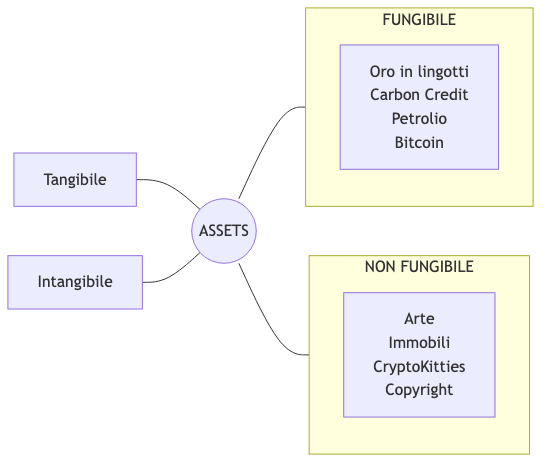
\includegraphics[keepaspectratio,alt={Diagramma Mermaid}]{images/mermaid-lezione-22-fungible-e-non-fungible-tokens-erc-standards-01.png}}
\emph{Fig. --- Tassonomia degli asset secondo fungibilità e tangibilità:
i token intangibili fungibili includono criptovalute e carbon credit,
quelli non fungibili includono arte digitale e copyright.}

Un NFT può rappresentare oggetti digitali unici come opere d'arte,
oggetti in-game, domini .eth; asset fisici come immobili o opere d'arte
reali (la tokenizzazione rende il trasferimento di proprietà più
efficiente riducendo il rischio di frodi); oppure certificati di
proprietà e identità. Il fenomeno dei \textbf{Beanie Babies} negli anni
'90 anticipa molte dinamiche degli NFT: produzione limitata, ritiro
deliberato di edizioni per creare scarsità, difetti intenzionali che
generano edizioni ultra-rare. La psicologia del collezionismo è la
stessa.

\begin{center}\rule{0.5\linewidth}{0.5pt}\end{center}

\section{Cryptographic Tokens e Standard
ERC}\label{cryptographic-tokens-e-standard-erc}

I token crittografici implementati come smart contract ereditano le
proprietà di tracciabilità, sicurezza e impossibilità di falsificazione
della blockchain. Il settore è in piena espansione: i \textbf{colored
coins} furono i primi cryptotoken sviluppati su Bitcoin; Ethereum rimane
la piattaforma dominante per via degli smart contract, ma esistono ora
piattaforme alternative specializzate.

\subsection{Perché uno standard?}\label{perchuxe9-uno-standard}

\begin{callouttip}{Il valore di uno standard}

Uno standard ERC garantisce ai developer che gli asset si comporteranno
in modo prevedibile, e alle aziende che i propri token saranno
compatibili con l'infrastruttura Ethereum esistente: wallet, exchange,
marketplace.

\end{callouttip}

\textbf{ERC} (\emph{Ethereum Request for Comment}, o \emph{Ethereum
Request for Improvements}) è il formato con cui si propongono e
approvano le specifiche degli smart contract. Uno standard ERC per i
token definisce l'interfaccia che un contratto deve implementare: come
vengono creati, trasferiti, mutati e distrutti i token. I tre standard
principali sono:

{\def\LTcaptype{none} % do not increment counter
\begin{longtable}[]{@{}
  >{\raggedright\arraybackslash}p{(\linewidth - 4\tabcolsep) * \real{0.3333}}
  >{\raggedright\arraybackslash}p{(\linewidth - 4\tabcolsep) * \real{0.3333}}
  >{\raggedright\arraybackslash}p{(\linewidth - 4\tabcolsep) * \real{0.3333}}@{}}
\toprule\noalign{}
\begin{minipage}[b]{\linewidth}\raggedright
Standard
\end{minipage} & \begin{minipage}[b]{\linewidth}\raggedright
Tipo
\end{minipage} & \begin{minipage}[b]{\linewidth}\raggedright
Caso d'uso principale
\end{minipage} \\
\midrule\noalign{}
\endhead
\bottomrule\noalign{}
\endlastfoot
\textbf{ERC-20} & Token fungibili & Criptovalute, governance, DeFi \\
\textbf{ERC-721} & Token non fungibili (NFT) & Arte digitale, oggetti da
collezione, immobili \\
\textbf{ERC-1155} & Multi-token (FT + NFT) & Gaming, piattaforme con
asset eterogenei \\
\end{longtable}
}

\begin{center}\rule{0.5\linewidth}{0.5pt}\end{center}

\section{ERC-20: Standard per Token
Fungibili}\label{erc-20-standard-per-token-fungibili}

Lo standard ERC-20 fu proposto dal co-fondatore di Ethereum Vitalik
Buterin nel novembre 2015. Definisce un insieme comune di funzioni che
ogni token fungibile su Ethereum deve implementare, così da garantire
l'interoperabilità con wallet, contratti e marketplace.

\subsection{Struttura interna: il balance
map}\label{struttura-interna-il-balance-map}

Il contratto ERC-20 mantiene internamente una struttura dati
fondamentale: un mapping da indirizzi a saldi.

\begin{verbatim}
balanceOf: address → uint256
\end{verbatim}

Il saldo di un indirizzo non è un numero astratto: dipende dal contratto
specifico e può rappresentare unità fisiche, diritti, valori monetari o
qualsiasi altra quantità che il contratto decida di modellare.

\subsection{Funzioni obbligatorie}\label{funzioni-obbligatorie}

Le sei funzioni obbligatorie dello standard sono:

{\def\LTcaptype{none} % do not increment counter
\begin{longtable}[]{@{}
  >{\raggedright\arraybackslash}p{(\linewidth - 2\tabcolsep) * \real{0.5000}}
  >{\raggedright\arraybackslash}p{(\linewidth - 2\tabcolsep) * \real{0.5000}}@{}}
\toprule\noalign{}
\begin{minipage}[b]{\linewidth}\raggedright
Funzione
\end{minipage} & \begin{minipage}[b]{\linewidth}\raggedright
Descrizione
\end{minipage} \\
\midrule\noalign{}
\endhead
\bottomrule\noalign{}
\endlastfoot
\texttt{totalSupply()} & Restituisce il totale di token attualmente
esistenti nel contratto. Può essere fisso o variabile. \\
\texttt{balanceOf(address)} & Restituisce il saldo di token di un
indirizzo specifico. \\
\texttt{transfer(address\ \_to,\ uint256\ \_value)} & Trasferisce token
dall'indirizzo del chiamante a \texttt{\_to}. \\
\texttt{approve(address\ \_spender,\ uint256\ \_value)} & Autorizza
\texttt{\_spender} a spendere al massimo \texttt{\_value} token per
conto del chiamante. \\
\texttt{allowance(address\ \_owner,\ address\ \_spender)} & Restituisce
la quota corrente approvata da \texttt{\_owner} per
\texttt{\_spender}. \\
\texttt{transferFrom(address\ \_from,\ address\ \_to,\ uint256\ \_value)}
& Trasferisce token da \texttt{\_from} a \texttt{\_to} per conto di un
delegato autorizzato. \\
\end{longtable}
}

Oltre alle funzioni, lo standard definisce due \textbf{eventi} che
devono essere emessi: -
\texttt{Transfer(address\ \_from,\ address\ \_to,\ uint256\ \_value)}
--- emesso a ogni trasferimento -
\texttt{Approval(address\ \_owner,\ address\ \_spender,\ uint256\ \_value)}
--- emesso a ogni approvazione

\subsection{Campi opzionali}\label{campi-opzionali}

I tre campi opzionali migliorano l'usabilità del token:

\begin{itemize}
\tightlist
\item
  \texttt{name()}: nome human-readable, ad es. \texttt{"US\ Dollars"}
\item
  \texttt{symbol()}: simbolo leggibile, ad es. \texttt{"USD"}
\item
  \texttt{decimals()}: numero di cifre decimali per la rappresentazione
  visiva. Solidity non supporta i numeri decimali --- lavora solo con
  interi --- per cui si rappresenta un valore con moltiplicatori. Con
  \texttt{decimals\ =\ 18}, il valore \texttt{1000000000000000000}
  corrisponde a \texttt{1.0} token a schermo.
\end{itemize}

\subsection{Meccanismo di trasferimento
diretto}\label{meccanismo-di-trasferimento-diretto}

La funzione \texttt{transfer} implementa una transazione diretta in un
solo passo: il proprietario del wallet invia token a un altro indirizzo,
esattamente come una transazione cryptocurrency convenzionale.

\begin{callouttip}{Transfer: Alice invia 10 token a Bob}

\begin{enumerate}
\def\labelenumi{\arabic{enumi}.}
\tightlist
\item
  Il wallet di Alice invia una transazione al contratto token, chiamando
  \texttt{transfer(BobAddress,\ 10)}
\item
  Il contratto aggiorna: \texttt{balanceOf{[}Alice{]}\ -=\ 10} e
  \texttt{balanceOf{[}Bob{]}\ +=\ 10}
\item
  Viene emesso l'evento \texttt{Transfer(Alice,\ Bob,\ 10)} on-chain,
  utile per il logging
\end{enumerate}

\end{callouttip}

\subsection{Meccanismo di delega
(Allowance)}\label{meccanismo-di-delega-allowance}

Il meccanismo di \textbf{allowance} risolve un problema pratico: in
molti scenari (pagamenti ricorrenti, marketplace, DeFi) è necessario che
una terza parte esegua transazioni per conto del proprietario, senza che
il proprietario debba approvare ogni singola operazione.

\pandocbounded{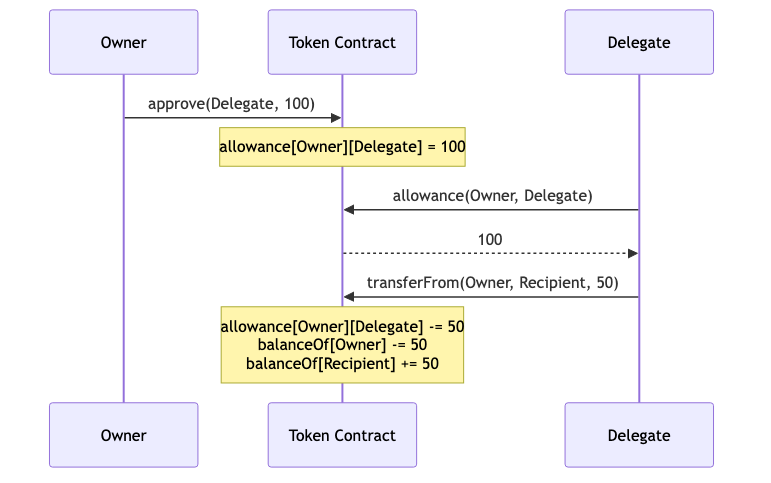
\includegraphics[keepaspectratio,alt={Diagramma Mermaid}]{images/mermaid-lezione-22-fungible-e-non-fungible-tokens-erc-standards-02.png}}
\emph{Fig. --- Flusso del meccanismo allowance: il proprietario approva
una quota, il delegato la utilizza con transferFrom.}

Il mapping interno che traccia le allowance è una struttura a due
livelli:

\begin{Shaded}
\begin{Highlighting}[]
\NormalTok{mapping(address =\textgreater{} mapping(address =\textgreater{} uint256)) public allowance;}
\end{Highlighting}
\end{Shaded}

La prima chiave è il proprietario, la seconda è lo spender autorizzato,
il valore è la quota massima. In altri termini:
\texttt{allowance{[}owner{]}{[}spender{]}} = quanto lo spender può
ancora spendere dal conto di owner.

\begin{callouttip}{Esempio completo di allowance}

Alice ha 1000 token e vuole delegare Bob a spenderne al massimo 100. 1.
Alice chiama \texttt{approve(Bob,\ 100)} 2. Bob verifica la quota con
\texttt{allowance(Alice,\ Bob)} → restituisce 100 3. Bob preleva 50
token: \texttt{transferFrom(Alice,\ Bob,\ 50)} → la allowance scende a
50 4. Bob può continuare a prelevare fino a esaurire la quota di 100
token totali

\end{callouttip}

\subsection{L'interfaccia IERC20 e
l'implementazione}\label{linterfaccia-ierc20-e-limplementazione}

L'interfaccia IERC20 formalizza in Solidity il contratto che ogni
implementazione ERC-20 deve rispettare:

\begin{Shaded}
\begin{Highlighting}[]
\NormalTok{// Funzioni opzionali}
\NormalTok{function name()     public view returns (string)  // optional}
\NormalTok{function symbol()   public view returns (string)  // optional}
\NormalTok{function decimals() public view returns (uint8)   // optional}

\NormalTok{// Funzioni obbligatorie}
\NormalTok{function totalSupply() public view returns (uint256)}
\NormalTok{function balanceOf(address \_owner) public view returns (uint256 balance)}
\NormalTok{function transfer(address \_to, uint256 \_value) public returns (bool success)}
\NormalTok{function approve(address \_spender, uint256 \_value) public returns (bool success)}
\NormalTok{function allowance(address \_owner, address \_spender) public view returns (uint256 remaining)}
\NormalTok{function transferFrom(address \_from, address \_to, uint256 \_value) public returns (bool success)}

\NormalTok{// Eventi}
\NormalTok{event Transfer(address indexed \_from, address indexed \_to, uint256 \_value)}
\NormalTok{event Approval(address indexed \_owner, address indexed \_spender, uint256 \_value)}
\end{Highlighting}
\end{Shaded}

Un'implementazione minimale del contratto ERC-20 è:

\begin{Shaded}
\begin{Highlighting}[]
\NormalTok{pragma solidity \^{}0.8.7;}
\NormalTok{contract MyToken \{}
\NormalTok{    string public name = "My Token";}
\NormalTok{    string public symbol = "MTK";}
\NormalTok{    uint8 public decimals = 18;}
\NormalTok{    uint public totalSupply = 100\_000 * 10**decimals;}
\NormalTok{    mapping(address =\textgreater{} uint) public balanceOf;}
\NormalTok{    mapping(address =\textgreater{} mapping(address =\textgreater{} uint)) public allowance;}

\NormalTok{    event Transfer(address indexed \_from, address indexed \_to, uint256 \_value);}
\NormalTok{    event Approval(address indexed \_owner, address indexed \_spender, uint256 \_value);}

\NormalTok{    function transfer(address \_to, uint256 \_value) public returns (bool success) \{}
\NormalTok{        balanceOf[msg.sender] {-}= \_value;}
\NormalTok{        balanceOf[\_to] += \_value;}
\NormalTok{        emit Transfer(msg.sender, \_to, \_value);}
\NormalTok{        return true;}
\NormalTok{    \}}

\NormalTok{    function approve(address \_spender, uint256 \_value) public returns (bool success) \{}
\NormalTok{        allowance[msg.sender][\_spender] = \_value;}
\NormalTok{        emit Approval(msg.sender, \_spender, \_value);}
\NormalTok{        return true;}
\NormalTok{    \}}

\NormalTok{    function transferFrom(address \_from, address \_to, uint256 \_value)}
\NormalTok{            public returns (bool success) \{}
\NormalTok{        require(allowance[\_from][msg.sender] \textgreater{}= \_value);}
\NormalTok{        balanceOf[\_from] {-}= \_value;}
\NormalTok{        balanceOf[\_to] += \_value;}
\NormalTok{        emit Transfer(\_from, \_to, \_value);}
\NormalTok{        allowance[\_from][msg.sender] {-}= \_value;}
\NormalTok{        return true;}
\NormalTok{    \}}
\NormalTok{\}}
\end{Highlighting}
\end{Shaded}

\begin{calloutwarning}{Bug nella slide originale}

Il codice presentato a lezione per \texttt{transferFrom} contiene un
errore: \texttt{balanceOf{[}\_from{]}\ +=\ \_value} invece di
\texttt{-=\ \_value}. La versione corretta sottrae il valore dal saldo
del mittente e lo aggiunge al destinatario.

\end{calloutwarning}

\begin{center}\rule{0.5\linewidth}{0.5pt}\end{center}

\section{Implementare i Token in
Solidity}\label{implementare-i-token-in-solidity}

\subsection{Contratti come classi, istanze e
deployment}\label{contratti-come-classi-istanze-e-deployment}

In Solidity, un contratto è concettualmente equivalente a una classe in
un linguaggio orientato agli oggetti. Il codice del contratto definisce
la struttura; l'\textbf{istanza} viene creata quando il contratto viene
deployato sulla blockchain tramite una transazione, a un determinato
indirizzo. Il creator può essere sia un external account che un altro
contratto (come mostrato nel pattern \emph{Fabric} che istanzia token
dinamicamente).

Una volta che un contratto crea un'istanza di un altro contratto tramite
\texttt{new}, l'istanza risultante può essere usata per invocare le
funzioni pubbliche dell'altro contratto:

\begin{Shaded}
\begin{Highlighting}[]
\NormalTok{Token token = new Token(\_name);   // deployment + riferimento}
\NormalTok{token.name();                     // invocazione funzione pubblica}
\end{Highlighting}
\end{Shaded}

\subsection{Ereditarietà}\label{ereditarietuxe0}

Solidity supporta l'ereditarietà in stile OOP. Un contratto figlio
eredita tutte le variabili di stato e le funzioni non dichiarate
\texttt{private} dal contratto padre. Le variabili e funzioni
\texttt{internal} sono accessibili nel contratto e nei derivati; quelle
\texttt{private} restano confinate al contratto in cui sono dichiarate,
rafforzando l'incapsulamento.

Le funzioni dichiarate \texttt{virtual} nel padre possono essere
sovrascritte nel figlio con \texttt{override}:

\begin{Shaded}
\begin{Highlighting}[]
\NormalTok{contract Foo \{}
\NormalTok{    function calculate(uint x, uint y) public virtual pure returns (uint) \{}
\NormalTok{        return x + y;}
\NormalTok{    \}}
\NormalTok{\}}
\NormalTok{contract Bar is Foo \{}
\NormalTok{    function calculate(uint x, uint y) public override pure returns (uint) \{}
\NormalTok{        return x {-} y;}
\NormalTok{    \}}
\NormalTok{\}}
\end{Highlighting}
\end{Shaded}

\subsection{Interfacce}\label{interfacce}

Le \textbf{interfacce} in Solidity sono blueprints puri: dichiarano le
firme delle funzioni senza implementarle e senza variabili di stato.
Sono lo strumento naturale per descrivere standard come ERC-20 ed
ERC-721, e possono ereditare da altre interfacce.

\subsection{OpenZeppelin: non reinventare la
ruota}\label{openzeppelin-non-reinventare-la-ruota}

\begin{callouttip}{OpenZeppelin}

OpenZeppelin (https://openzeppelin.com) è un SDK open source per lo
sviluppo sicuro di smart contract. Il codice è sottoposto ad auditing
continuo dalla community e usato in circa 3000 progetti blockchain.
Fornisce template pronti per ERC-20, ERC-721 ed ERC-1155 importabili
direttamente.

\end{callouttip}

\begin{Shaded}
\begin{Highlighting}[]
\NormalTok{import "@openzeppelin/contracts/token/ERC20/ERC20.sol";}
\NormalTok{contract MyToken is ERC20 \{}
\NormalTok{    constructor() ERC20("MyToken", "MTK") \{}
\NormalTok{        \_mint(msg.sender, 1000);}
\NormalTok{    \}}
\NormalTok{\}}
\end{Highlighting}
\end{Shaded}

\texttt{MyToken} è un contratto figlio di \texttt{ERC20} di
OpenZeppelin, ne eredita tutte le funzioni. Il costruttore del padre
richiede nome e simbolo del token, che devono essere trasmessi dal
figlio. La funzione \texttt{\_mint} crea token dal nulla e li assegna
all'indirizzo specificato, incrementando di conseguenza il
\texttt{totalSupply}.

\begin{center}\rule{0.5\linewidth}{0.5pt}\end{center}

\section{ERC-721: Standard per NFT}\label{erc-721-standard-per-nft}

Lo standard ERC-721 fu proposto nel gennaio 2018. La differenza
architetturale rispetto a ERC-20 è fondamentale: mentre ERC-20 mappa
\textbf{indirizzi → quantità}, ERC-721 mappa \textbf{ID unici →
proprietari}.

\begin{calloutdefinition}{tokenId in ERC-721}

Ogni NFT è identificato da un \texttt{uint256\ tokenId}. La coppia
\texttt{(contract\ address,\ tokenId)} deve essere \textbf{globalmente
unica}: il tokenId è univoco all'interno di un contratto. Due contratti
ERC-721 diversi possono avere token con lo stesso ID numerico, ma non
rappresentano lo stesso asset.

\end{calloutdefinition}

L'interfaccia ERC-721 offre funzionalità analoghe a ERC-20 ma adattate
alla gestione di token unici:

\begin{Shaded}
\begin{Highlighting}[]
\NormalTok{function balanceOf(address \_owner) external view returns (uint256);}
\NormalTok{function ownerOf(uint256 \_tokenId) external view returns (address);}
\NormalTok{function safeTransferFrom(address \_from, address \_to, uint256 \_tokenId, bytes data) external payable;}
\NormalTok{function safeTransferFrom(address \_from, address \_to, uint256 \_tokenId) external payable;}
\NormalTok{function transferFrom(address \_from, address \_to, uint256 \_tokenId) external payable;}
\NormalTok{function approve(address \_approved, uint256 \_tokenId) external payable;}
\NormalTok{function setApprovalForAll(address \_operator, bool \_approved) external;}
\NormalTok{function getApproved(uint256 \_tokenId) external view returns (address);}
\NormalTok{function isApprovedForAll(address \_owner, address \_operator) external view returns (bool);}
\end{Highlighting}
\end{Shaded}

\subsection{safeTransferFrom: perché
esiste}\label{safetransferfrom-perchuxe9-esiste}

La funzione \texttt{transferFrom} standard presenta un problema critico:
trasferisce il token senza verificare se il contratto destinatario sia
in grado di gestire NFT. Se l'indirizzo \texttt{\_to} è uno smart
contract che non implementa il supporto ERC-721, il token viene inviato
e si blocca permanentemente, irrecuperabile.

Per questo motivo esiste \texttt{safeTransferFrom}, che aggiunge un
controllo: 1. Se \texttt{\_to} è un contratto, chiama
\texttt{onERC721Received(...)} su di esso 2. Se il contratto non
implementa correttamente questa funzione (cioè non ``riconosce'' il
token ricevuto), la transazione viene revertita 3. Il trasferimento
avviene solo se il destinatario dimostra di saper gestire NFT

\begin{calloutwarning}{Gli NFT sono preziosi}

Usare \texttt{transferFrom} invece di \texttt{safeTransferFrom} verso un
contratto sconosciuto è rischioso: se il contratto destinatario non
supporta ERC-721, l'NFT va perso per sempre. Preferire sempre
\texttt{safeTransferFrom} quando il destinatario potrebbe essere un
contratto.

\end{calloutwarning}

\begin{center}\rule{0.5\linewidth}{0.5pt}\end{center}

\section{Metadata degli NFT}\label{metadata-degli-nft}

Un NFT non è solo un ID on-chain: il suo valore deriva dai
\textbf{metadata} associati, ovvero le informazioni che descrivono cosa
rappresenta.

\subsection{La struttura dei metadata}\label{la-struttura-dei-metadata}

I metadati tipici di un NFT includono:

{\def\LTcaptype{none} % do not increment counter
\begin{longtable}[]{@{}
  >{\raggedright\arraybackslash}p{(\linewidth - 2\tabcolsep) * \real{0.5000}}
  >{\raggedright\arraybackslash}p{(\linewidth - 2\tabcolsep) * \real{0.5000}}@{}}
\toprule\noalign{}
\begin{minipage}[b]{\linewidth}\raggedright
Campo
\end{minipage} & \begin{minipage}[b]{\linewidth}\raggedright
Significato
\end{minipage} \\
\midrule\noalign{}
\endhead
\bottomrule\noalign{}
\endlastfoot
\texttt{name} & Nome dell'NFT (es. ``Cool Ape \#123'') \\
\texttt{description} & Descrizione testuale \\
\texttt{image} & Link all'immagine (IPFS o HTTP) \\
\texttt{attributes} & Array di trait\_type/value per caratteristiche
specifiche \\
\texttt{unlockable\_content} & Contenuto accessibile solo al
proprietario \\
\texttt{royalty} & Percentuale di royalty per rivendite future \\
\texttt{supply} & Quasi sempre 1 per gli NFT \\
\end{longtable}
}

\subsection{tokenURI: il collegamento tra on-chain e
metadata}\label{tokenuri-il-collegamento-tra-on-chain-e-metadata}

La funzione \texttt{tokenURI(uint256\ tokenId)} è il punto di accesso ai
metadata: dato un tokenId, restituisce un URI che punta a un file JSON.
Questo URI può essere un URL HTTP
(\texttt{https://my-nft-site.com/metadata/123.json}) oppure un link IPFS
(\texttt{ipfs://Qm.../123.json}). Il file JSON contiene a sua volta
ulteriori link, tra cui il link all'immagine vera e propria.

\pandocbounded{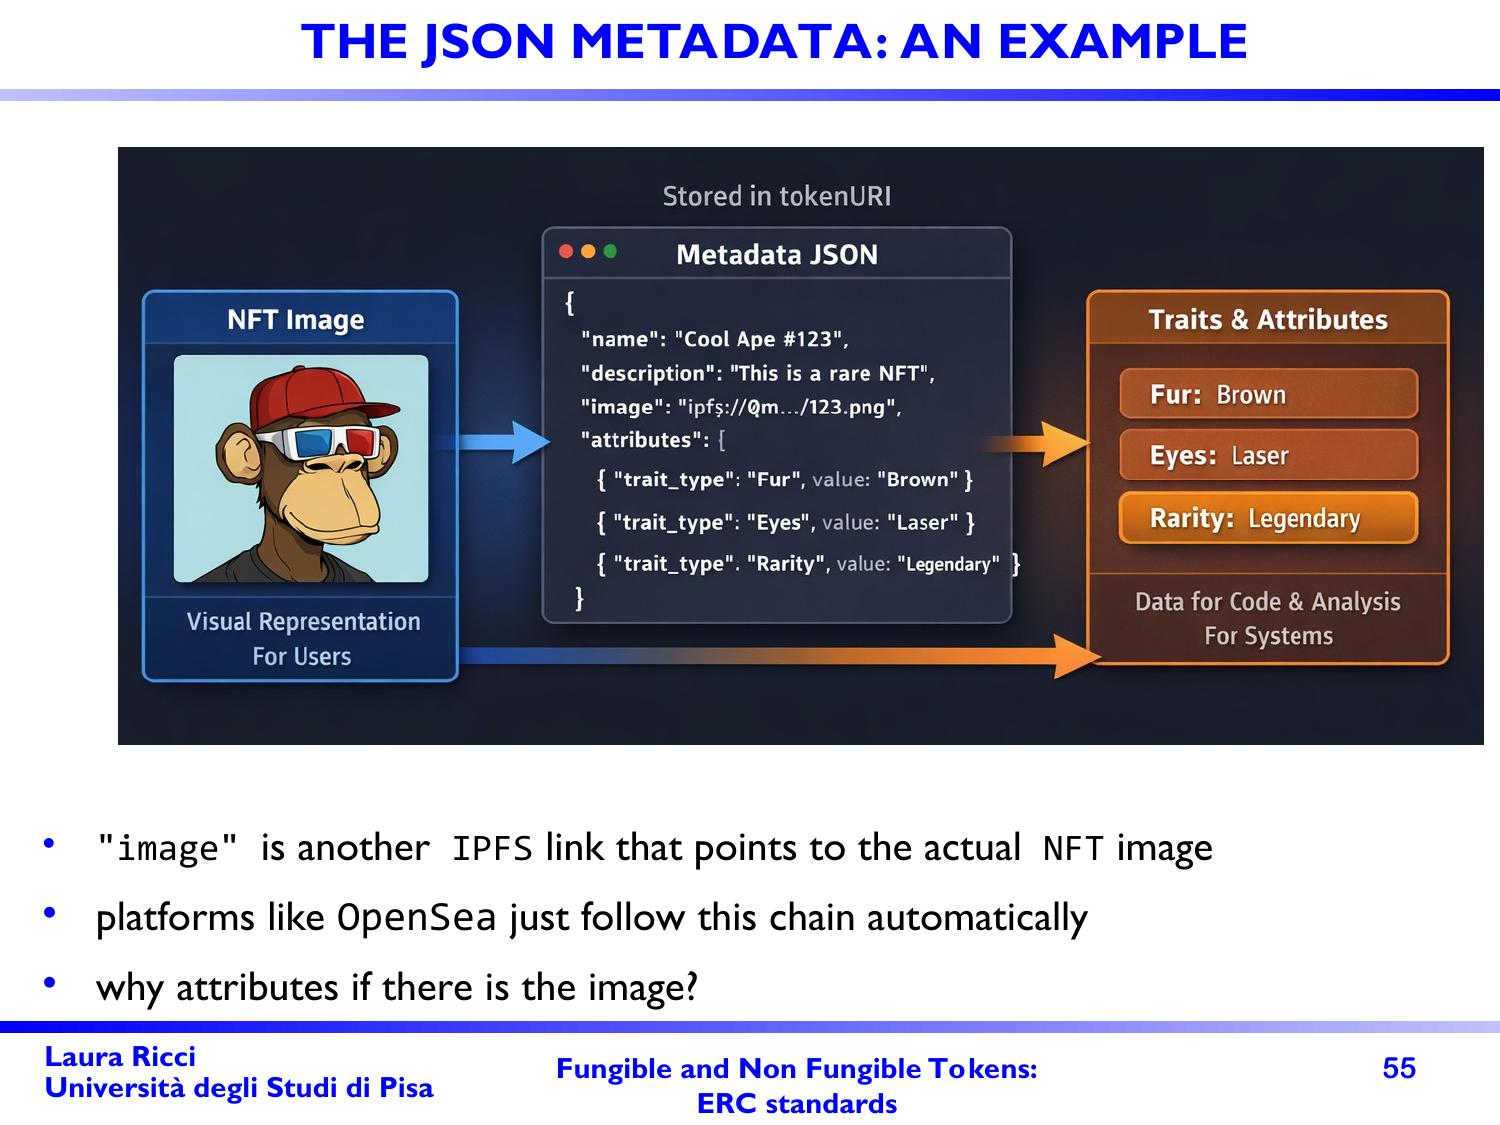
\includegraphics[keepaspectratio,alt={Schema del flusso NFT Image → JSON Metadata → Traits \& Attributes}]{images/lezione-22-fungible-e-non-fungible-tokens-erc-standards-img-01.jpg}}
\emph{Fig. --- Il flusso dei metadata di un NFT: la \texttt{tokenURI}
punta al JSON, che contiene il link IPFS all'immagine e l'array di
attributi usati da marketplace e sistemi per filtrare e calcolare la
rarità.}

\subsection{Perché gli attributi se c'è
l'immagine?}\label{perchuxe9-gli-attributi-se-cuxe8-limmagine}

L'immagine è per gli umani; gli attributi sono per le macchine. I
marketplace come OpenSea usano gli attributi per permettere il
\textbf{filtro} (\emph{``solo NFT con fur dorata''}), il \textbf{calcolo
della rarità} (\emph{se solo l'1\% ha ``Laser Eyes'', quell'attributo è
molto raro e aumenta il valore}) e la \textbf{logica di gioco}
(\emph{uno Strength di 85 può influenzare il gameplay}). Senza attributi
strutturati, un marketplace potrebbe solo mostrare le immagini, non
filtrarle.

\subsection{On-chain vs Off-chain: dove archiviare i
metadata?}\label{on-chain-vs-off-chain-dove-archiviare-i-metadata}

Archiviare i metadata direttamente on-chain è possibile ma costosissimo
e raramente raccomandato. Si fa solo quando: - L'informazione deve
persistere indipendentemente dall'esistenza del sito originale (arte
digitale destinata a durare secoli) - La logica del contratto deve
accedere ai metadata (es. l'età dei CryptoKitties influenza la velocità
di riproduzione)

La soluzione off-chain prevalente è l'\textbf{IPFS}
(\emph{InterPlanetary File System}), una rete peer-to-peer
decentralizzata dove i contenuti sono distribuiti su più nodi e
indirizzati per contenuto (non per posizione). L'alternativa cloud (AWS,
Google Cloud) esiste ma contraddice lo spirito decentralizzato della
blockchain.

\subsection{Royalties}\label{royalties}

Le royalties permettono all'autore originale di un NFT di ricevere una
percentuale automatica su ogni rivendita futura, senza dover fare nulla.
Il contratto traccia la percentuale scelta dall'artista e, ogni volta
che l'NFT cambia mano, invia automaticamente la quota al wallet del
creatore.

\pandocbounded{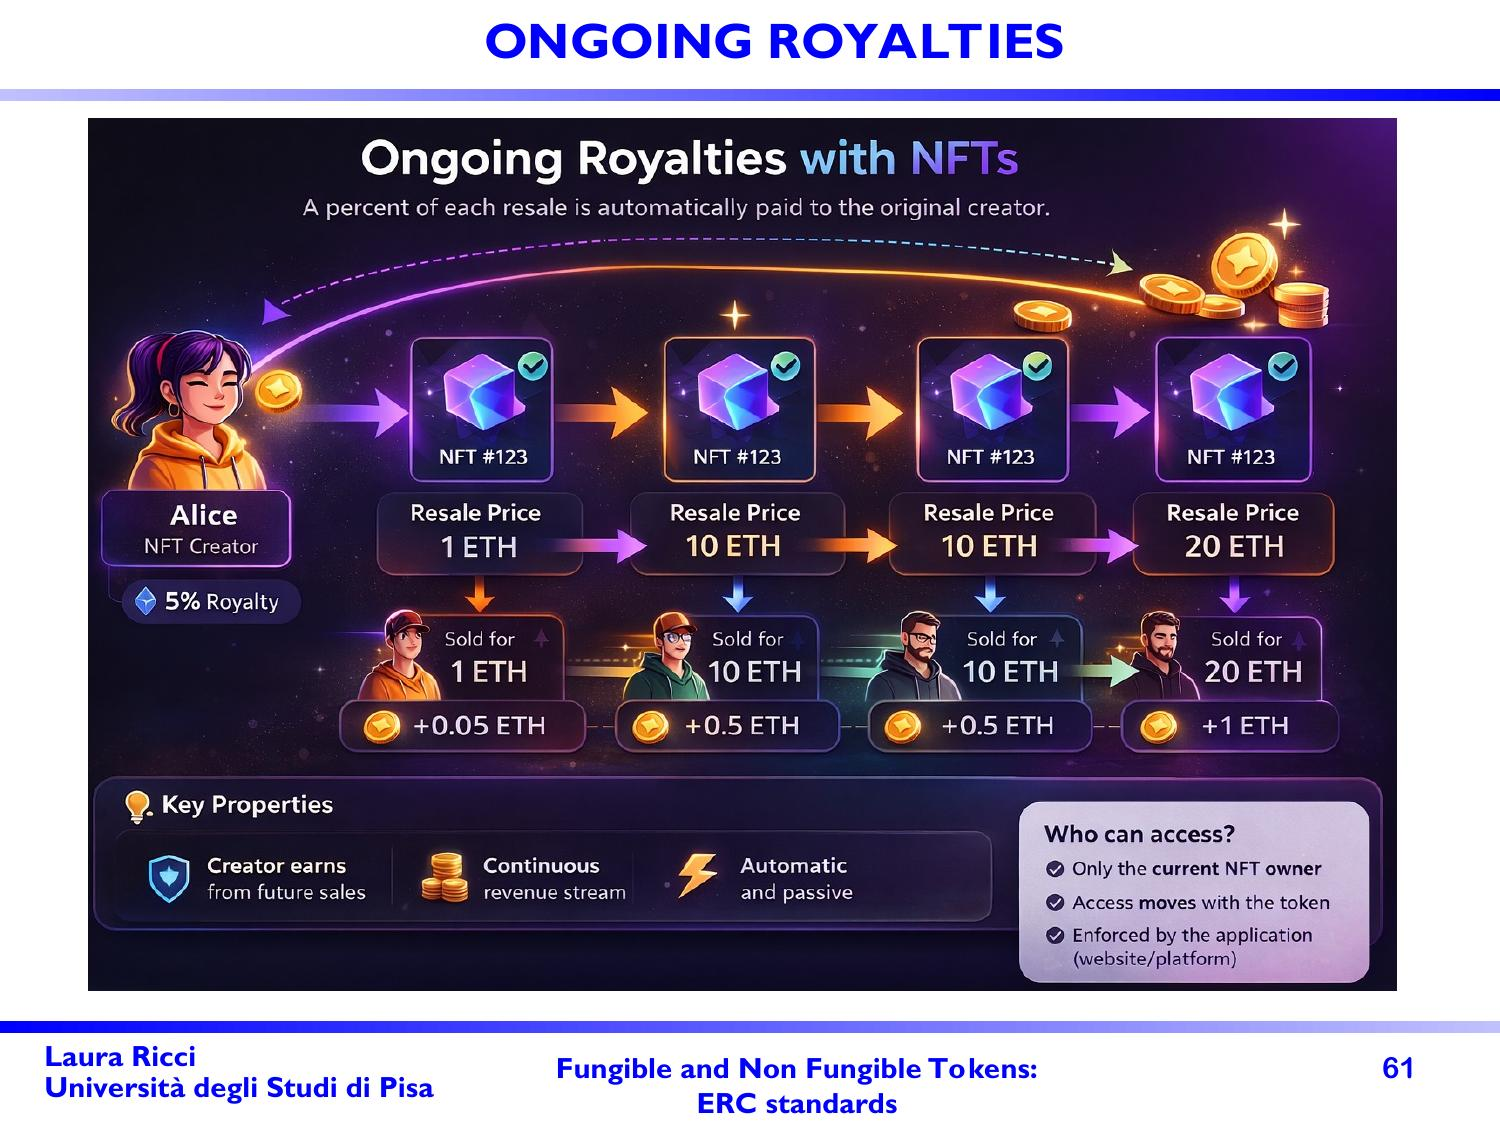
\includegraphics[keepaspectratio,alt={Infografica sulle ongoing royalties con NFT}]{images/lezione-22-fungible-e-non-fungible-tokens-erc-standards-img-02.jpg}}
\emph{Fig. --- Il meccanismo delle royalties: Alice crea e vende NFT
\#123 per 1 ETH con royalty del 5\%. Ad ogni rivendita futura (10 ETH,
10 ETH, 20 ETH), Alice riceve automaticamente il 5\% --- rispettivamente
0.05, 0.5, 0.5, 1 ETH --- senza alcuna azione da parte sua.}

\subsection{Unlockable Content}\label{unlockable-content}

L'\emph{unlockable content} è contenuto visibile o accessibile solo al
proprietario corrente dell'NFT: video esclusivi, documenti privati,
codici di attivazione, access key per community ristrette. L'accesso si
sposta automaticamente con il token quando viene trasferito.

Il flusso di verifica che una piattaforma deve implementare è:

\pandocbounded{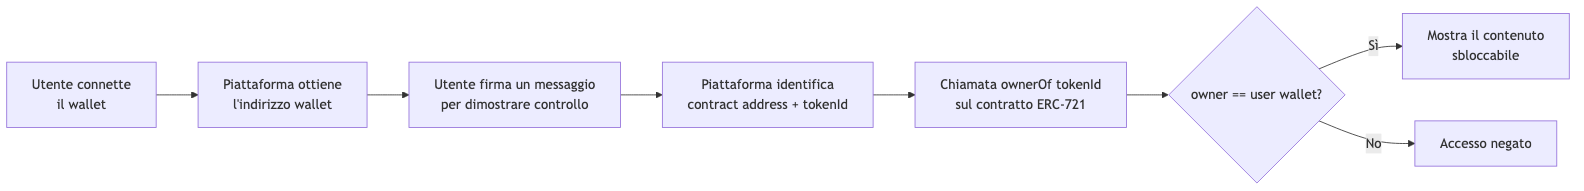
\includegraphics[keepaspectratio,alt={Diagramma Mermaid}]{images/mermaid-lezione-22-fungible-e-non-fungible-tokens-erc-standards-03.png}}
\emph{Fig. --- Flusso di verifica per l'unlockable content: la
piattaforma chiama \texttt{ownerOf(tokenId)} on-chain e confronta il
risultato con il wallet connesso dall'utente.}

\begin{center}\rule{0.5\linewidth}{0.5pt}\end{center}

\section{ERC-20 vs ERC-721: il confronto
strutturale}\label{erc-20-vs-erc-721-il-confronto-strutturale}

La differenza architetturale tra i due standard si riassume in come
viene organizzato il registro interno:

\pandocbounded{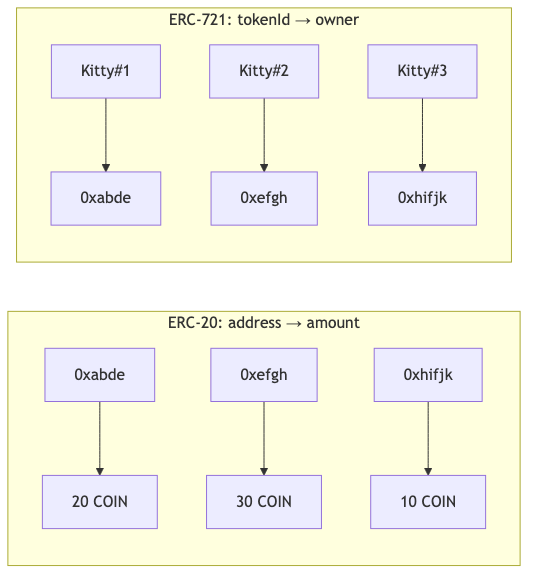
\includegraphics[keepaspectratio,alt={Diagramma Mermaid}]{images/mermaid-lezione-22-fungible-e-non-fungible-tokens-erc-standards-04.png}}
\emph{Fig. --- ERC-20 mappa indirizzi a quantità (fungibile); ERC-721
mappa ID unici a proprietari (non fungibile).}

\begin{center}\rule{0.5\linewidth}{0.5pt}\end{center}

\section{ERC-1155: Multi-Token
Standard}\label{erc-1155-multi-token-standard}

Lo standard ERC-1155 fu proposto dal CTO di Enjin nel 2018 con un
obiettivo preciso: \textbf{ridurre il volume di transazioni e i costi}
combinando in un unico contratto le funzionalità di ERC-20 e ERC-721.

\begin{calloutdefinition}{ERC-1155}

Un singolo contratto ERC-1155 può gestire contemporaneamente token
fungibili (come ERC-20) e token non fungibili (come ERC-721),
supportando il \textbf{batch transfer} (trasferimento di più token in
una sola transazione) e includendo meccanismi di safe transfer per
prevenire perdite.

\end{calloutdefinition}

Il confronto tra ERC-721 ed ERC-1155 evidenzia i vantaggi di
quest'ultimo:

{\def\LTcaptype{none} % do not increment counter
\begin{longtable}[]{@{}
  >{\raggedright\arraybackslash}p{(\linewidth - 4\tabcolsep) * \real{0.3333}}
  >{\raggedright\arraybackslash}p{(\linewidth - 4\tabcolsep) * \real{0.3333}}
  >{\raggedright\arraybackslash}p{(\linewidth - 4\tabcolsep) * \real{0.3333}}@{}}
\toprule\noalign{}
\begin{minipage}[b]{\linewidth}\raggedright
Caratteristica
\end{minipage} & \begin{minipage}[b]{\linewidth}\raggedright
ERC-721
\end{minipage} & \begin{minipage}[b]{\linewidth}\raggedright
ERC-1155
\end{minipage} \\
\midrule\noalign{}
\endhead
\bottomrule\noalign{}
\endlastfoot
Tipi di token supportati & Solo NFT & FT e NFT \\
Smart contract richiesti & Uno per ogni tipo di token & Uno solo per
tutti i tipi \\
Batch transfer & Non supportato & Supportato (meno gas, meno
transazioni) \\
Safe transfer & No recovery se indirizzo sbagliato & Verifica +
possibilità di recovery \\
\end{longtable}
}

\subsection{Applicazioni di ERC-1155}\label{applicazioni-di-erc-1155}

Il gaming è il caso d'uso principale. \textbf{Enjin Platform} usa
ERC-1155 per creare asset di gioco --- armi, scudi, oggetti ---
gestibili in un unico contratto condiviso tra più giochi. \textbf{The
Sandbox} usa ERC-1155 per terreni, edifici e attrezzature nel suo
metaverso. \textbf{Rarible} lo usa per supportare sia FT che NFT sulla
stessa piattaforma, aumentando la flessibilità per artisti e
collezionisti.

\begin{center}\rule{0.5\linewidth}{0.5pt}\end{center}

\section{La ``giungla'' degli standard
ERC}\label{la-giungla-degli-standard-erc}

\begin{calloutnote}{Un ecosistema in espansione}

ERC-20, ERC-721 ed ERC-1155 sono i principali standard, ma l'ecosistema
Ethereum ne conta molti altri: ERC-777 (valuta Ethereum-based), ERC-827
(trasferimento a terze parti), ERC-884 (stock tokenization),
ERC-1400/1404 (security token), ERC-725 (identità digitale), ERC-223
(European Research Council standard). La proliferazione di standard
riflette la ricchezza e complessità degli use case che la tokenizzazione
rende possibili.

\end{calloutnote}

\newpage

\chapter{Lab 8 --- Advanced Solidity: Vulnerabilities e Contract
Upgrading}\label{lab-8-advanced-solidity-vulnerabilities-e-contract-upgrading}

Questa lezione chiude il ciclo su Solidity affrontando due temi che
separano il codice didattico dal codice production-ready: le
\textbf{vulnerabilità tipiche} degli smart contract e le
\textbf{strategie di aggiornamento} per contratti che, per natura,
nascono immutabili. I due temi sono strettamente collegati:
l'impossibilità di correggere un contratto dopo il deploy rende le
vulnerabilità particolarmente dannose, e i pattern di upgrading sono
nati proprio per mitigare questa rigidità --- al prezzo, però, di
introdurre nuove forme di centralizzazione e nuovi vettori di attacco.

\begin{callouttip}{Filosofia della lezione}

In Ethereum il codice è legge, ma la legge può contenere bachi. Scrivere
smart contract sicuri significa anticipare i modi in cui un attaccante
può manipolare il contesto di esecuzione (chi chiama, quando, con quale
gas, con quali effetti collaterali) e progettare il codice perché non
dipenda da invarianti che l'attaccante può violare.

\end{callouttip}

\begin{center}\rule{0.5\linewidth}{0.5pt}\end{center}

\section{Vulnerabilità comuni}\label{vulnerabilituxe0-comuni}

Prima di entrare nei singoli pattern di attacco è utile fissare alcune
considerazioni generali, valide trasversalmente per qualsiasi contratto
che gestisca valore o logica critica.

\subsection{Caveat generali}\label{caveat-generali}

Due insidie ricorrenti, spesso sottovalutate, riguardano la
\textbf{generazione di casualità} e il \textbf{costo delle view
function}.

La prima questione nasce dal fatto che, in un sistema deterministico e
replicato come l'EVM, non esiste una vera sorgente di casualità interna
alla blockchain. Qualsiasi valore apparentemente casuale (hash di un
blocco, timestamp, difficulty) è in realtà \textbf{manipolabile dai
validatori}, che possono scegliere di non produrre il blocco se l'esito
non è loro favorevole --- o di ritardarne la pubblicazione per estrarre
valore. Un contratto che dipenda da ``casualità on-chain'' per decisioni
economicamente rilevanti (lotterie, estrazioni, distribuzione di premi)
è vulnerabile per costruzione. Le soluzioni vere richiedono oracoli
specializzati con schemi commit-reveal o VRF (Verifiable Random
Functions) come Chainlink VRF.

La seconda questione è più sottile. Una funzione marcata \texttt{view}
non modifica lo stato e, \textbf{se chiamata esternamente da fuori la
blockchain} (ad esempio via \texttt{eth\_call} da una DApp), non costa
gas. Tuttavia, se la stessa funzione viene chiamata \textbf{da un'altra
funzione on-chain}, il suo costo viene sommato al gas della transazione
che la contiene. Una view function con loop non limitato su una
struttura dati che cresce nel tempo può quindi diventare un
\textbf{denial-of-service economico}: inizialmente gratuita, poi
progressivamente più costosa, fino a superare il block gas limit.

\begin{calloutwarning}{Le view function non sono “gratis” in assoluto}

\texttt{view} garantisce solo che la funzione non scriva sullo stato.
Non garantisce che il costo di lettura sia limitato. Se un altro
contratto la chiama, paga l'esecuzione. Un attaccante può \textbf{far
crescere volutamente} strutture dati iterate dalle view per trasformarle
in bombe a orologeria.

\end{calloutwarning}

\begin{calloutnote}{Riferimenti della lezione}

La guida ufficiale Ethereum sui disaster recovery plans e la sezione
sicurezza degli smart contract è disponibile su
\texttt{ethereum.org/developers/docs/smart-contracts/security}. Per
esercitarsi sui pattern di attacco è storicamente utile
\textbf{Ethernaut} (\texttt{ethernaut.openzeppelin.com}), una CTF di
OpenZeppelin sui bug classici: leggermente datato, ma ancora ottimo per
allenare l'istinto difensivo.

\end{calloutnote}

\subsection{Overflows}\label{overflows}

Gli overflow aritmetici sono stati a lungo il bug più classico di
Solidity. In una \texttt{uint256} l'operazione
\texttt{type(uint256).max\ +\ 1} tornava silenziosamente a \texttt{0},
con effetti disastrosi quando il valore rappresentava un saldo o un
contatore critico. La libreria \textbf{SafeMath} di OpenZeppelin è nata
proprio per fornire operazioni aritmetiche con controllo esplicito e
revert in caso di overflow.

Dalla versione \textbf{0.8.0} del compilatore Solidity, il controllo di
overflow/underflow è diventato \textbf{automatico} per tutte le
operazioni aritmetiche standard. Il compilatore inserisce istruzioni di
verifica che fanno revert della transazione se il risultato uscisse dai
limiti del tipo. SafeMath rimane storicamente rilevante ma, in pratica,
l'uso è diventato marginale: i contratti moderni possono fare
affidamento sul controllo automatico, a meno che non sia esplicitamente
necessario l'overflow silente (nel qual caso si usa un blocco
\texttt{unchecked\ \{\ ...\ \}} per disattivarlo localmente e
risparmiare gas).

\begin{callouttip}{Quando usare unchecked}

Il blocco \texttt{unchecked} serve quando si è \textbf{matematicamente
certi} che l'overflow non possa avvenire (es. una variabile di loop
limitata, un decremento protetto da un \texttt{require} precedente) e si
vuole evitare il costo del check automatico. Usarlo per errore è
esattamente il tipo di bug che il controllo automatico è stato
introdotto per prevenire.

\end{callouttip}

\subsection{\texorpdfstring{Phishing tramite
\texttt{tx.origin}}{Phishing tramite tx.origin}}\label{phishing-tramite-tx.origin}

Solidity espone due variabili globali che a prima vista sembrano
intercambiabili: \texttt{msg.sender} e \texttt{tx.origin}. La differenza
è cruciale. \texttt{msg.sender} è l'indirizzo dell'\textbf{ultimo
chiamante} --- il contratto o l'EOA (Externally Owned Account) che ha
invocato direttamente la funzione corrente. \texttt{tx.origin} è invece
l'indirizzo dell'\textbf{EOA che ha firmato la transazione} all'origine
dell'intera catena di chiamate.

Un controllo di autorizzazione basato su \texttt{tx.origin} è
vulnerabile a un classico attacco \textbf{man-in-the-middle}: un
contratto malevolo può indurre la vittima (che magari è l'owner di un
contratto protetto) a interagire con sé, e poi, durante quella stessa
transazione, invocare il contratto protetto. A quel punto
\texttt{tx.origin} è ancora l'indirizzo della vittima (che ha firmato la
transazione), quindi il controllo passa, anche se l'effettivo chiamante
immediato (\texttt{msg.sender}) è il contratto malevolo.

\pandocbounded{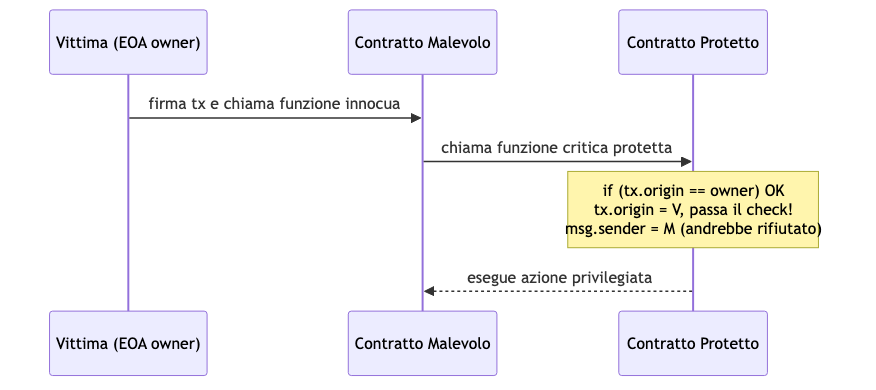
\includegraphics[keepaspectratio,alt={Diagramma Mermaid}]{images/mermaid-lezione-23-lab-advanced-solidity-vulnerabilities-e-upgrading-01.png}}
\emph{Fig. --- Schema dell'attacco di phishing basato su
\texttt{tx.origin}: l'EOA della vittima resta \texttt{tx.origin} lungo
tutta la catena di chiamate, quindi il controllo ingannevole passa
nonostante il vero chiamante sia un contratto ostile.}

\begin{calloutwarning}{Regola pratica}

\textbf{Non usare mai \texttt{tx.origin} per controlli di
autorizzazione.} Usa sempre \texttt{msg.sender}. L'unico uso legittimo
di \texttt{tx.origin} è il rifiuto deliberato di chiamate da parte di
contratti (\texttt{require(tx.origin\ ==\ msg.sender)}), pattern oggi
considerato scarsamente utile perché fragile e anti-composizionale.

\end{calloutwarning}

\subsection{Reentrancy}\label{reentrancy}

La reentrancy è probabilmente la vulnerabilità più famosa della storia
di Ethereum --- è il bug che nel 2016 portò al collasso di \textbf{The
DAO} e alla hard fork che separò Ethereum da Ethereum Classic. L'essenza
del problema è semplice: si verifica quando \textbf{una funzione (o una
combinazione di funzioni) viene richiamata dall'interno della propria
esecuzione}, prima che gli effetti della prima chiamata siano stati
consolidati nello stato del contratto.

Il vettore tipico è una chiamata esterna a un contratto non fidato:
l'EVM, per \texttt{.call()}, \texttt{send} o \texttt{transfer} verso un
indirizzo di contratto, esegue il codice del \textbf{fallback} o della
\texttt{receive} di quel contratto. Se il fallback a sua volta richiama
la funzione originaria, e questa non ha ancora aggiornato lo stato che
regola l'accesso, l'attaccante può ottenere più volte il risultato di
un'operazione che avrebbe dovuto essere unica.

\subsubsection{Esempio classico: withdraw
vulnerabile}\label{esempio-classico-withdraw-vulnerabile}

\begin{Shaded}
\begin{Highlighting}[]
\NormalTok{function withdraw() public \{}
\NormalTok{    require(shares[msg.sender] \textgreater{} 0);}

\NormalTok{    (bool success,) = msg.sender.call\{value: shares[msg.sender]\}("");}

\NormalTok{    if (success)}
\NormalTok{        shares[msg.sender] = 0;}
\NormalTok{\}}
\end{Highlighting}
\end{Shaded}

Il problema è l'\textbf{ordine delle operazioni}. La funzione:

\begin{enumerate}
\def\labelenumi{\arabic{enumi}.}
\tightlist
\item
  verifica che il chiamante abbia share positive,
\item
  invia l'ether corrispondente (che trigger-a eventualmente il fallback
  del chiamante),
\item
  \textbf{solo dopo} azzera le share.
\end{enumerate}

Se il chiamante è un contratto il cui fallback chiama di nuovo
\texttt{withdraw()}, al passo 1 della seconda invocazione il controllo
\texttt{shares{[}msg.sender{]}\ \textgreater{}\ 0} passa ancora (le
share non sono state azzerate), e il contratto invia di nuovo ether. Il
processo si ripete fino a svuotare il contratto o esaurire il gas della
transazione.

\pandocbounded{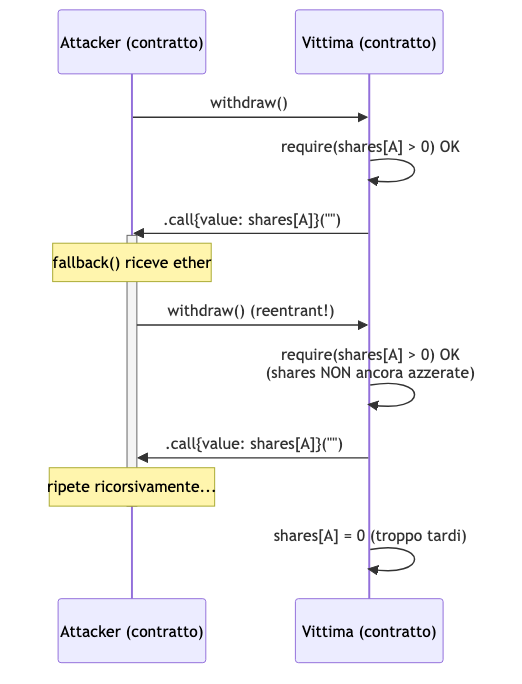
\includegraphics[keepaspectratio,alt={Diagramma Mermaid}]{images/mermaid-lezione-23-lab-advanced-solidity-vulnerabilities-e-upgrading-02.png}}
\emph{Fig. --- Il flusso di una reentrancy classica: la chiamata esterna
restituisce il controllo al contratto malevolo, che rientra nella
funzione prima che lo stato sia aggiornato.}

\subsubsection{Mitigazioni}\label{mitigazioni}

La difesa principale è il pattern \textbf{Checks-Effects-Interactions}:
prima si fanno tutti i \textbf{controlli} (\texttt{require}), poi si
aggiornano \textbf{gli effetti} sullo stato locale, e \textbf{solo alla
fine} si eseguono le \textbf{interazioni} con contratti esterni.
Riscritto correttamente, l'esempio diventa:

\begin{Shaded}
\begin{Highlighting}[]
\NormalTok{function withdraw() public \{}
\NormalTok{    uint256 amount = shares[msg.sender];}
\NormalTok{    require(amount \textgreater{} 0);}
\NormalTok{    shares[msg.sender] = 0;                          // Effect prima}
\NormalTok{    (bool success,) = msg.sender.call\{value: amount\}("");}
\NormalTok{    require(success);}
\NormalTok{\}}
\end{Highlighting}
\end{Shaded}

Ora, anche se il fallback del chiamante richiama \texttt{withdraw}, il
check fallisce perché \texttt{shares{[}msg.sender{]}} è già 0.

Esistono mitigazioni complementari, meno robuste ma utili come difesa in
profondità:

\begin{itemize}
\tightlist
\item
  \textbf{Limitare il gas della chiamata esterna} (usando \texttt{send}
  o \texttt{transfer}, che forniscono solo 2300 gas, o fissando un gas
  cap in \texttt{call}). È una mitigazione storica che però non è sempre
  applicabile: dopo l'EIP-1884 il costo di alcune operazioni è aumentato
  e i 2300 gas di \texttt{transfer} possono non bastare per fallback
  legittimi, rompendo l'interoperabilità.
\item
  \textbf{Lock non-reentrant} (reentrancy guard): un mutex booleano che
  viene alzato all'ingresso di funzioni sensibili e abbassato
  all'uscita. Se una chiamata esterna prova a rientrare, il mutex è alto
  e il require fallisce. OpenZeppelin fornisce
  \texttt{ReentrancyGuardTransient} (versione ottimizzata con storage
  transient EIP-1153) e \texttt{ReentrancyGuard}. \textbf{Attenzione a
  non rimanere bloccati per sempre}: il mutex deve essere abbassato in
  ogni percorso di uscita, inclusi i revert gestiti.
\end{itemize}

\begin{callouttip}{Reentrancy guard con modifier}

\begin{Shaded}
\begin{Highlighting}[]
\NormalTok{bool private locked;}
\NormalTok{modifier nonReentrant() \{}
\NormalTok{    require(!locked, "Reentrant call");}
\NormalTok{    locked = true;}
\NormalTok{    \_;}
\NormalTok{    locked = false;}
\NormalTok{\}}
\end{Highlighting}
\end{Shaded}

Applicando \texttt{nonReentrant} alla funzione \texttt{withdraw},
qualunque rientro trova \texttt{locked\ ==\ true} e viene rifiutato.

\end{callouttip}

\begin{calloutnote}{Approfondimenti}

Un'analisi dettagliata del TheDAO exploit si trova su
\texttt{medium.com/@zhongqiangc/smart-contract-reentrancy-thedao-f2da1d25180c}.
Una raccolta sistematica di attacchi reentrancy è mantenuta in
\texttt{github.com/pcaversaccio/reentrancy-attacks}. Il guard ufficiale
OpenZeppelin è su
\texttt{github.com/OpenZeppelin/openzeppelin-contracts/blob/master/contracts/utils/ReentrancyGuardTransient.sol}.

\end{calloutnote}

\begin{center}\rule{0.5\linewidth}{0.5pt}\end{center}

\section{Contract Upgrading}\label{contract-upgrading}

Gli smart contract su Ethereum sono \textbf{immutabili per design}: una
volta deployato il bytecode, non esiste un'istruzione EVM per
modificarlo. Questa proprietà è sia una forza (garantisce che il codice
non possa essere alterato dopo il deploy) sia un limite (non permette di
correggere bachi né di aggiungere funzionalità). Il \textbf{contract
upgrading} è l'insieme dei pattern architetturali che consentono di
aggirare questa rigidità quando è necessario.

\subsection{Perché (e perché no) aggiornare un
contratto}\label{perchuxe9-e-perchuxe9-no-aggiornare-un-contratto}

I benefici dell'upgradability sono evidenti: permette di
\textbf{correggere vulnerabilità o bachi} scoperti dopo il deploy,
\textbf{aggiungere nuove funzionalità} che rispondano a requisiti
emergenti, e predisporre \textbf{disaster recovery plans} per
intervenire in caso di attacco o malfunzionamento grave.

Il costo è altrettanto concreto: un contratto upgradable è, per
definizione, \textbf{meno immutabile}, quindi meno credibilmente
neutrale. Introduce un potere centralizzato (chi controlla l'upgrade?)
che può essere usato maliziosamente o compromesso. L'upgrade stesso è
una superficie di attacco: un nuovo contratto logic può introdurre bug o
backdoor non presenti nella versione originale.

La mitigazione standard è introdurre \textbf{timelock} (ritardi
obbligatori tra annuncio e attivazione di un upgrade, per dare agli
utenti tempo di uscire) e \textbf{multisig} (richiedere più firme per
autorizzare l'upgrade, evitando single-point-of-failure sulla chiave del
deployer). Il trade-off è evidente: i timelock rallentano le risposte in
emergenza, i multisig aumentano il costo operativo. È un compromesso,
non una soluzione.

\begin{callouttip}{L’upgradability come scelta politica}

Rendere un contratto upgradable è anche una dichiarazione di governance:
chi può votare l'upgrade? Con quale maggioranza? Dopo quanto tempo?
Molti protocolli DeFi hanno migrato nel tempo da multisig a DAO
governance proprio per decentralizzare questo potere.

\end{callouttip}

\subsection{Esempio guida della
lezione}\label{esempio-guida-della-lezione}

Come filo conduttore la lezione usa l'aggiunta di funzionalità di
\textbf{``proper deactivation''} al posto di \texttt{selfdestruct} come
disaster recovery plan: si parte dal contratto \texttt{Created.sol} e si
trasforma in \texttt{CreatedSafe.sol}, ragionando su come far adottare
la nuova logica senza rompere lo stato già esistente.

\subsection{Le quattro opzioni
principali}\label{le-quattro-opzioni-principali}

Esistono due macrofamiglie di soluzioni --- quelle \textbf{senza proxy}
e quelle \textbf{con proxy} --- per un totale di quattro pattern
principali:

\pandocbounded{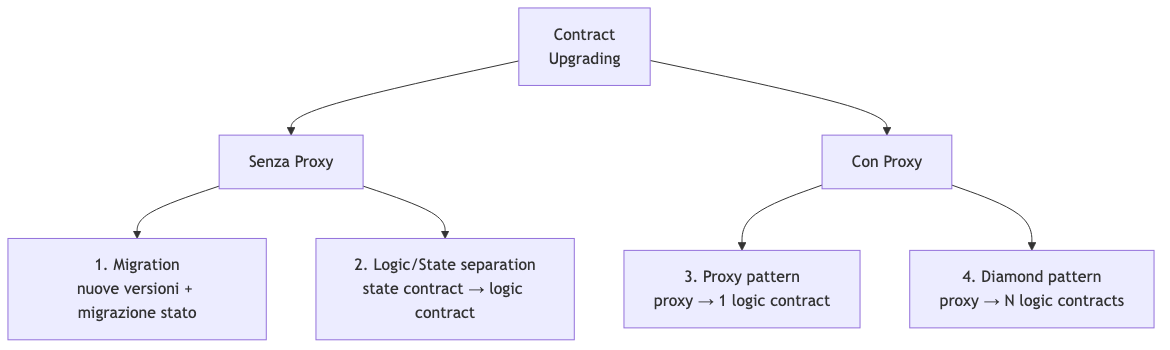
\includegraphics[keepaspectratio,alt={Diagramma Mermaid}]{images/mermaid-lezione-23-lab-advanced-solidity-vulnerabilities-e-upgrading-03.png}}
\emph{Fig. --- Tassonomia delle strategie di upgrading: si parte dalla
scelta se introdurre o meno un proxy, e all'interno di ciascuna famiglia
si distinguono approcci monolitici e modulari.}

\subsubsection{Opzione 1 --- Migration}\label{opzione-1-migration}

Si crea una \textbf{nuova istanza} del contratto con la logica
aggiornata e si \textbf{migrano i dati} dal vecchio al nuovo. È
l'approccio più semplice concettualmente, ma impone che \textbf{tutti
gli utenti passino al nuovo contratto}: ogni DApp, ogni wallet, ogni
interazione esterna deve essere aggiornata al nuovo indirizzo. Rompe
ogni integrazione on-chain che avesse hard-coded il vecchio indirizzo.
Funziona bene per contratti di nicchia con pochi utenti coordinabili,
male per protocolli con ampia adozione.

\subsubsection{Opzione 2 --- Separazione
logic/state}\label{opzione-2-separazione-logicstate}

Si divide il contratto in due: un \textbf{contratto di stato}
(immutabile, contiene i dati) e un \textbf{contratto di logica}
(mutabile, contiene il codice). Il contratto di stato espone
getter/setter accessibili solo dal contratto di logica corrente, e
mantiene un puntatore al contratto di logica attivo, aggiornabile dal
proprietario.

Il vantaggio è che i dati non si spostano mai: lo stato rimane nello
stesso indirizzo. Lo svantaggio è che \textbf{il caller interagisce con
l'indirizzo della logica}, quindi un cambio di logica cambia l'indirizzo
con cui l'utente interagisce --- e le DApp devono aggiornarsi. È una
mezza soluzione: risolve il problema della migrazione dati ma non quello
dello stable address.

\subsubsection{Opzione 3 --- Proxy
pattern}\label{opzione-3-proxy-pattern}

È l'approccio più diffuso nei protocolli moderni. Si usa un
\textbf{proxy contract immutabile} che l'utente chiama sempre allo
stesso indirizzo. Il proxy non contiene logica di business: contiene
solo una \textbf{puntatore al contratto logic} e una funzione
\texttt{fallback} che \textbf{delegate-call}-a al logic contract ogni
invocazione ricevuta.

La chiave è \texttt{delegatecall}: a differenza di \texttt{call}, esegue
il codice del callee \textbf{nel contesto (storage) del caller}. Quindi
lo stato vive nel proxy, ma l'implementazione viene letta dal logic.
Aggiornare il contratto significa cambiare il puntatore del proxy verso
un nuovo logic contract.

\pandocbounded{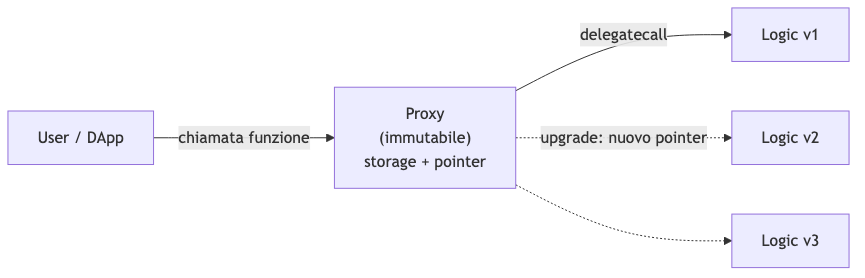
\includegraphics[keepaspectratio,alt={Diagramma Mermaid}]{images/mermaid-lezione-23-lab-advanced-solidity-vulnerabilities-e-upgrading-04.png}}
\emph{Fig. --- Pattern proxy: l'utente interagisce sempre con lo stesso
indirizzo (il proxy), ma la logica eseguita è quella del contratto
puntato, sostituibile dall'owner.}

\begin{calloutdefinition}{delegatecall}

Opcode EVM che esegue il codice di un altro contratto \textbf{nel
contesto di storage, \texttt{msg.sender} e \texttt{msg.value} del
caller}. A differenza di \texttt{call}, che esegue il callee nel proprio
contesto, \texttt{delegatecall} tratta il codice del callee come una
libreria: lo stato modificato è quello del caller. È il meccanismo
fondamentale che rende possibile il pattern proxy.

\end{calloutdefinition}

L'implementazione di riferimento è \texttt{Proxy.sol} di OpenZeppelin,
disponibile in
\texttt{github.com/OpenZeppelin/openzeppelin-contracts/blob/v4.8.2/contracts/proxy/Proxy.sol}.
Un tutorial pratico è
\texttt{jamesbachini.com/proxy-contracts-tutorial/}.

\begin{calloutwarning}{Storage collision}

Il punto più delicato del pattern proxy è l'\textbf{allineamento dello
storage}: proxy e logic devono avere layout di storage compatibili,
perché entrambi scrivono nello stesso storage (quello del proxy). Se il
logic v2 aggiunge una variabile nel mezzo della lista, tutte le
variabili successive ``scorrono'' e vengono sovrascritte/lette da slot
sbagliati. Per questo OpenZeppelin impone un layout di storage
\textbf{append-only} e usa slot deterministici (EIP-1967) per le
variabili del proxy stesso (come l'indirizzo dell'implementazione), così
da non collidere con quelle della logic.

\end{calloutwarning}

\subsubsection{\texorpdfstring{Sintassi Solidity: \texttt{virtual},
\texttt{override},
\texttt{abstract}}{Sintassi Solidity: virtual, override, abstract}}\label{sintassi-solidity-virtual-override-abstract}

Il pattern proxy usa intensivamente l'ereditarietà, quindi richiede
familiarità con tre parole chiave:

{\def\LTcaptype{none} % do not increment counter
\begin{longtable}[]{@{}
  >{\raggedright\arraybackslash}p{(\linewidth - 2\tabcolsep) * \real{0.5000}}
  >{\raggedright\arraybackslash}p{(\linewidth - 2\tabcolsep) * \real{0.5000}}@{}}
\toprule\noalign{}
\begin{minipage}[b]{\linewidth}\raggedright
Parola chiave
\end{minipage} & \begin{minipage}[b]{\linewidth}\raggedright
Significato
\end{minipage} \\
\midrule\noalign{}
\endhead
\bottomrule\noalign{}
\endlastfoot
\texttt{virtual} & Il metodo \textbf{può essere sovrascritto} da un
contratto che eredita. \\
\texttt{override} & Il metodo \textbf{sta sovrascrivendo} un metodo
\texttt{virtual} del contratto padre. \\
\texttt{abstract} & Il contratto \textbf{non può essere istanziato}
direttamente perché ha funzioni/parametri non implementati; serve solo
come base per sottoclassi. \\
\end{longtable}
}

Il concetto di \texttt{abstract} è analogo a Java: un contratto che
dichiara firme di funzioni senza implementazione, lasciando ai derivati
il compito di completarlo.

\subsubsection{Opzione 4 --- Diamond pattern
(EIP-2535)}\label{opzione-4-diamond-pattern-eip-2535}

Il pattern proxy standard ha un limite: \textbf{un solo logic contract}
alla volta. Ma un logic contract è un singolo contratto Solidity, quindi
è soggetto al \textbf{limite di dimensione del bytecode} (circa 24 KB
per EIP-170). Protocolli grandi (DEX, lending, derivati) rischiano di
sbattere contro questo soffitto.

Il \textbf{diamond pattern} (EIP-2535) generalizza il proxy: un unico
contratto ``diamond'' (immutabile, con lo stato) delega a \textbf{più
logic contracts}, detti \textbf{facets}. Ogni selector di funzione (i 4
byte che identificano una funzione nell'ABI) è mappato al facet che la
implementa. Quando un utente chiama una funzione, il diamond consulta la
mappa, individua il facet competente, e delegate-call-a ad esso.

\pandocbounded{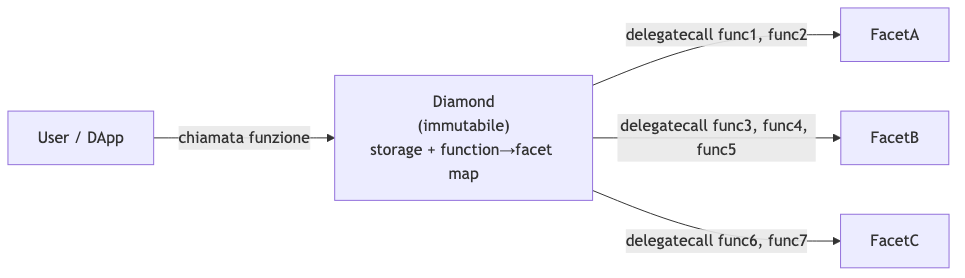
\includegraphics[keepaspectratio,alt={Diagramma Mermaid}]{images/mermaid-lezione-23-lab-advanced-solidity-vulnerabilities-e-upgrading-05.png}}
\emph{Fig. --- Pattern diamond: un unico indirizzo esposto all'utente,
ma le funzioni sono implementate da più facet. La mappatura funzione →
facet è aggiornabile, permettendo di sostituire, aggiungere o rimuovere
facet nel tempo.}

Il cuore del pattern è la \textbf{function-to-facet mapping}:

\begin{Shaded}
\begin{Highlighting}[]
\NormalTok{mapping(bytes4 =\textgreater{} address) facets;}

\NormalTok{// Esempio di mapping:}
\NormalTok{// (func1) e2532512 =\textgreater{} 0x0b22380B7c423470...  (FacetA)}
\NormalTok{// (func2) b1e5392a =\textgreater{} 0x0b22380B7c423470...  (FacetA)}
\NormalTok{// (func3) 1857ea99 =\textgreater{} 0x501E5D8e2FBbBc8A...  (FacetB)}
\NormalTok{// (func4) 876e3abc =\textgreater{} 0x501E5D8e2FBbBc8A...  (FacetB)}
\NormalTok{// (func5) 79d9df55 =\textgreater{} 0x501E5D8e2FBbBc8A...  (FacetB)}
\NormalTok{// (func6) 0b7eac44 =\textgreater{} 0x39555988230b4c87...  (FacetC)}
\NormalTok{// (func7) d86e6291 =\textgreater{} 0x39555988230b4c87...  (FacetC)}
\end{Highlighting}
\end{Shaded}

Il diamond gestisce anche più \textbf{storage struct} dedicate (una per
facet o gruppo di facet), tipicamente usando il pattern \textbf{Diamond
Storage} per isolare gli slot di storage di ciascun facet ed evitare
collisioni: ogni facet usa uno slot di storage calcolato come hash di
una stringa unica, garantendo che facet diversi non si pestino i piedi.

\begin{callouttip}{Perché “diamond”}

Il nome richiama la forma dell'ereditarietà multipla: un singolo punto
di ingresso (il diamond) si apre su molte facce (i facet). A differenza
dell'ereditarietà multipla tradizionale, qui non c'è un unico albero di
compilazione: i facet sono contratti separati, deployati
indipendentemente, e la ``composizione'' avviene a runtime tramite la
mappa di selector. Il risultato è massima modularità, al prezzo di una
maggiore complessità di governance (ora bisogna gestire upgrade,
aggiunte e rimozioni di facet).

\end{callouttip}

\begin{calloutnote}{Sintesi dei quattro pattern}

{\def\LTcaptype{none} % do not increment counter
\begin{longtable}[]{@{}
  >{\raggedright\arraybackslash}p{(\linewidth - 8\tabcolsep) * \real{0.2000}}
  >{\raggedright\arraybackslash}p{(\linewidth - 8\tabcolsep) * \real{0.2000}}
  >{\raggedright\arraybackslash}p{(\linewidth - 8\tabcolsep) * \real{0.2000}}
  >{\raggedright\arraybackslash}p{(\linewidth - 8\tabcolsep) * \real{0.2000}}
  >{\raggedright\arraybackslash}p{(\linewidth - 8\tabcolsep) * \real{0.2000}}@{}}
\toprule\noalign{}
\begin{minipage}[b]{\linewidth}\raggedright
Opzione
\end{minipage} & \begin{minipage}[b]{\linewidth}\raggedright
Indirizzo stabile?
\end{minipage} & \begin{minipage}[b]{\linewidth}\raggedright
Migrazione dati?
\end{minipage} & \begin{minipage}[b]{\linewidth}\raggedright
Complessità
\end{minipage} & \begin{minipage}[b]{\linewidth}\raggedright
Limite dimensione
\end{minipage} \\
\midrule\noalign{}
\endhead
\bottomrule\noalign{}
\endlastfoot
Migration & no & sì & bassa & nessuno \\
Logic/state separation & no (cambia logic) & no & media &
\textasciitilde24 KB \\
Proxy & \textbf{sì} & no & media & \textasciitilde24 KB \\
Diamond & \textbf{sì} & no & alta & \textbf{nessuno} (molti facet) \\
\end{longtable}
}

\end{calloutnote}

\begin{center}\rule{0.5\linewidth}{0.5pt}\end{center}

\section{Mappa concettuale della
lezione}\label{mappa-concettuale-della-lezione}

\pandocbounded{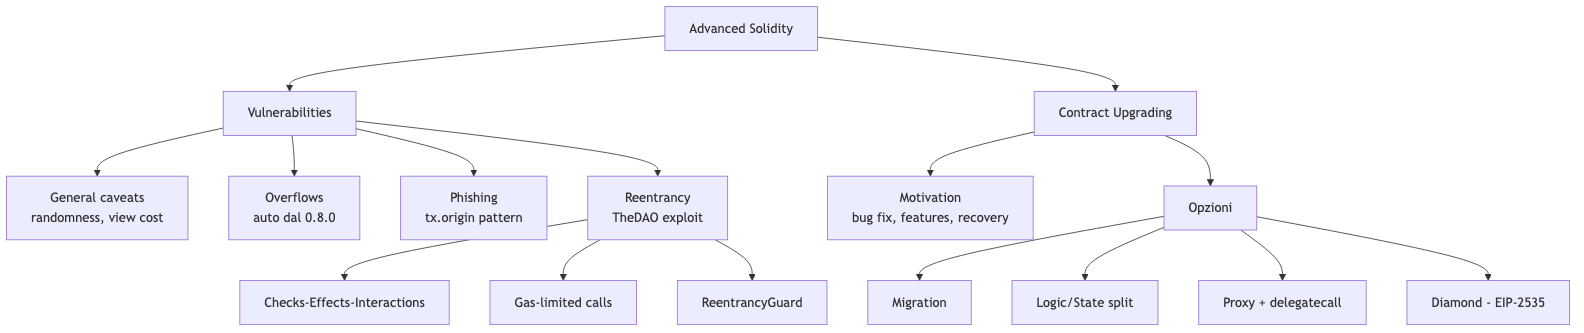
\includegraphics[keepaspectratio,alt={Diagramma Mermaid}]{images/mermaid-lezione-23-lab-advanced-solidity-vulnerabilities-e-upgrading-06.png}}
\emph{Fig. --- Struttura complessiva della lezione: da un lato i pattern
di attacco e le relative difese, dall'altro l'evoluzione dei pattern
architetturali per superare l'immutabilità degli smart contract.}

\begin{center}\rule{0.5\linewidth}{0.5pt}\end{center}

\newpage

\chapter{IPFS: Interplanetary File
System}\label{ipfs-interplanetary-file-system}

\section{Il Web centralizzato e il problema della
localizzazione}\label{il-web-centralizzato-e-il-problema-della-localizzazione}

Il Web così come lo conosciamo oggi si regge su un modello
\textbf{location based}: quando scriviamo
\texttt{http://sito.com/image.jpg} non stiamo chiedendo ``voglio quella
specifica immagine'', bensì ``contatta la macchina che risponde a
\texttt{sito.com} e chiedigli il file \texttt{image.jpg}''. L'indirizzo
HTTP punta cioè a un \textbf{luogo} della rete --- un dominio risolto in
un indirizzo IP, che a sua volta identifica una macchina fisica. La
conseguenza è duplice: il contenuto esiste solo fintanto che quel server
è raggiungibile, e l'intero modello è fragile rispetto alla censura, ai
guasti e alla centralizzazione delle infrastrutture.

\begin{calloutwarning}{Il problema della censura}

Se un governo o un provider decide di bloccare un dominio o un indirizzo
IP, il contenuto diventa irraggiungibile per intere porzioni di rete,
anche se copie dello stesso file sono fisicamente presenti su milioni di
macchine sparse nel mondo. Il legame forte fra \textbf{contenuto} e
\textbf{luogo} è ciò che rende possibile la censura su scala.

\end{calloutwarning}

C'è inoltre un problema più sottile di \emph{discovery}: immagina che
Mary voglia una certa immagine e che Bob, sulla stessa rete locale, ce
l'abbia già sul disco. Nel modello HTTP, Mary non ha alcun modo di
sapere che il file è a due metri da lei: deve per forza contattare il
web server d'origine, magari dall'altra parte del mondo. Manca un
meccanismo che permetta di \textbf{recuperare il contenuto da dove esso
si trova}, invece che da dove è stato pubblicato.

\subsection{Dal Web location-based al Web
content-based}\label{dal-web-location-based-al-web-content-based}

L'idea di IPFS è ribaltare la prospettiva: invece di indirizzare il
\emph{contenitore} (il server), si indirizza direttamente il
\emph{contenuto}. Non ci interessa sapere dove un file è ospitato, ci
interessa solo \textbf{che cosa è} quel file. Se riusciamo a dare a ogni
file un nome univoco derivato dal suo contenuto, allora la rete può
occuparsi autonomamente di cercarlo dove esso si trova, replicarlo,
servirlo dal nodo più vicino.

\begin{callouttip}{Intuizione chiave: content addressing}

In un sistema \textbf{content-addressed}, il nome di un file \emph{è} il
file --- nel senso che è una funzione univoca dei suoi bit. Due file
identici hanno lo stesso nome, ovunque essi siano; un file manomesso
anche in un singolo bit ha un nome diverso. La localizzazione diventa un
problema di rete, non di design del protocollo.

\end{callouttip}

\begin{center}\rule{0.5\linewidth}{0.5pt}\end{center}

\section{IPFS: cos'è e da dove
viene}\label{ipfs-cosuxe8-e-da-dove-viene}

IPFS (\textbf{InterPlanetary File System}) è un protocollo peer-to-peer
per lo storage distribuito dei contenuti del Web, sviluppato da
\textbf{Protocol Labs}. Lo slogan canonico, tratto dal white paper di
Juan Benet del 2013, lo descrive come un ``Content Addressed, Versioned,
P2P File System''. Il contributo di IPFS, secondo lo stesso Benet, non è
inventare nuove tecniche, ma \emph{combinare} in un unico sistema
coerente idee già collaudate nel mondo peer-to-peer.

\begin{calloutnote}{L’ecosistema di Protocol Labs}

\begin{itemize}
\tightlist
\item
  \textbf{IPFS} --- protocollo P2P content-based, alternativa a HTTP per
  lo scambio di contenuti.
\item
  \textbf{Filecoin} --- rete di storage decentralizzata con un mercato
  basato su criptovaluta, costruita \emph{sopra} IPFS per risolvere il
  problema degli incentivi allo storage.
\item
  \textbf{libp2p} --- libreria modulare di rete nata come sotto-progetto
  di IPFS e poi diventata indipendente, usata da molti altri progetti.
\end{itemize}

\end{calloutnote}

Le idee che IPFS riprende e integra sono:

{\def\LTcaptype{none} % do not increment counter
\begin{longtable}[]{@{}
  >{\raggedright\arraybackslash}p{(\linewidth - 2\tabcolsep) * \real{0.5000}}
  >{\raggedright\arraybackslash}p{(\linewidth - 2\tabcolsep) * \real{0.5000}}@{}}
\toprule\noalign{}
\begin{minipage}[b]{\linewidth}\raggedright
Componente
\end{minipage} & \begin{minipage}[b]{\linewidth}\raggedright
Ispirazione
\end{minipage} \\
\midrule\noalign{}
\endhead
\bottomrule\noalign{}
\endlastfoot
Routing & DHT (con miglioramenti da \textbf{S/Kademlia} per la sicurezza
e \textbf{Coral sloppy DHT} per la performance) \\
Strutture dati & \textbf{Merkle DAG} (da Git e dai Merkle tree
crittografici) \\
Scambio di blocchi & \textbf{BitTorrent}, adattato nel protocollo
\textbf{Bitswap} \\
Versionamento & \textbf{Git} (version control system) \\
Namespace auto-certificante & \textbf{SFS} (Self-Certified File
System) \\
\end{longtable}
}

Nessuno di questi è un nodo ``privilegiato'': la rete IPFS è piatta,
ogni peer memorizza oggetti nel proprio store locale e si connette ad
altri peer per trasferire blocchi. L'identificazione dei contenuti è
\textbf{content-based tramite hash crittografico sicuro}, lo scambio è
peer-to-peer in stile BitTorrent, l'organizzazione dei file segue un
\textbf{DAG di Merkle} che permette al tempo stesso verifica
crittografica, deduplicazione e versionamento.

\begin{center}\rule{0.5\linewidth}{0.5pt}\end{center}

\section{Lo stack di IPFS a colpo
d'occhio}\label{lo-stack-di-ipfs-a-colpo-docchio}

Prima di entrare nei dettagli, è utile avere in mente l'architettura a
livelli di IPFS. Il sistema si presenta come uno stack, in cui ogni
livello si appoggia a quello sottostante e risolve un problema distinto.

\pandocbounded{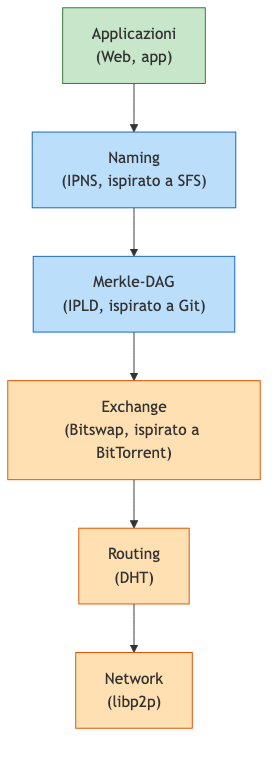
\includegraphics[keepaspectratio,alt={Diagramma Mermaid}]{images/mermaid-lezione-24-ipfs-interplanetary-file-system-01.png}}
\emph{Fig. --- Lo stack IPFS: il livello più basso trasporta i dati
(network, routing, exchange), quello intermedio li definisce
(Merkle-DAG, naming), quello superiore li usa (applicazioni).}

Tre blocchi logici emergono chiaramente. In basso troviamo
\textbf{Transporting Data}, il compito di muovere bit tra peer: network
(libp2p), routing (DHT), exchange (Bitswap). Al centro \textbf{Defining
Data}, dove i bit diventano strutture identificabili: Merkle-DAG e
naming (IPNS). In cima \textbf{Using Data}, dove le applicazioni si
appoggiano a tutto il resto.

\begin{center}\rule{0.5\linewidth}{0.5pt}\end{center}

\section{Content addressing: l'hashing come
indirizzo}\label{content-addressing-lhashing-come-indirizzo}

L'idea fondativa di IPFS è trasformare ogni pezzo di contenuto in un
identificatore derivato matematicamente dai suoi bit. Quando carichi una
foto su IPFS, accade questo: l'immagine viene convertita in raw data
(una sequenza di byte), e su questi byte viene calcolato un \textbf{hash
crittografico sicuro} --- per default \textbf{SHA-256}, ma
l'architettura supporta esplicitamente l'uso di altri algoritmi (e
vedremo fra poco perché questa flessibilità è cruciale). Il digest
risultante diventa l'etichetta univoca del contenuto.

\begin{calloutdefinition}{Hash crittografico come indirizzo}

Un hash crittografico è una funzione che mappa input di qualsiasi
lunghezza in output di lunghezza fissa (256 bit per SHA-256), con tre
proprietà fondamentali: \textbf{tamper-freeness} (cambiare un bit
dell'input cambia drasticamente l'output), \textbf{verifiability}
(chiunque può ricalcolare l'hash e verificare l'integrità del dato) e
\textbf{security} (non è possibile risalire all'input dall'output).

\end{calloutdefinition}

Queste tre proprietà si traducono direttamente in tre garanzie di IPFS.
La prima è \textbf{l'auto-certificazione}: se Bob ti invia un file
dichiarando che ha un certo CID, basta ricalcolare l'hash per verificare
che non sia stato manomesso --- non serve fidarsi di Bob. La seconda è
\textbf{l'integrità end-to-end}: se anche un singolo pixel di una foto
viene modificato, il suo hash cambia completamente, quindi il CID
corrispondente è diverso. La terza è \textbf{la robustezza contro la
manipolazione}: non esistendo un modo efficiente per costruire un file
diverso con lo stesso hash, IPFS è di fatto un file system a prova di
tampering.

\subsection{Dal digest al CID (Content
Identifier)}\label{dal-digest-al-cid-content-identifier}

Il digest da solo, però, non basta. Per poter evolvere l'algoritmo di
hashing nel tempo, supportare formati di codifica diversi e permettere a
software differenti di interpretare correttamente i dati, IPFS non usa
\emph{l'hash puro} come indirizzo: lo avvolge in una struttura chiamata
\textbf{CID (Content Identifier)}.

\begin{calloutdefinition}{Content Identifier (CID)}

Un CID è un'identificazione \textbf{self-describing} del contenuto.
Contiene:

\begin{itemize}
\tightlist
\item
  \textbf{l'hash del contenuto} --- che identifica \emph{cosa} è il
  dato;
\item
  \textbf{metadata} che descrivono \emph{come} interpretare/decodificare
  il dato (quale algoritmo di hash, quale codifica, quale formato di
  serializzazione).
\end{itemize}

Il CID \textbf{non} indica dove il contenuto è memorizzato: non è un
puntatore di rete, è un'\,``impronta digitale'' auto-descrittiva.

\end{calloutdefinition}

Nelle versioni legacy, i CID cominciano con il prefisso \texttt{Qm…}
(es. \texttt{QmPK1s3pNYLi9ERiq3BDxKa4XosgWwFRQUydHUtz4YgpqB}). Le
versioni moderne (CIDv1) hanno una struttura più flessibile e ricca, che
analizzeremo a breve.

\begin{center}\rule{0.5\linewidth}{0.5pt}\end{center}

\section{Il progetto Multiformat}\label{il-progetto-multiformat}

La scelta di includere i metadata dentro il CID nasce da un'esigenza
molto concreta di \textbf{evoluzione del software}. Se hard-codifichi
SHA-256 ovunque nel tuo codice, il giorno in cui SHA-256 viene rotto
(come è successo a MD5, e come potrebbe succedere domani con l'arrivo di
computer più potenti o con attacchi crittografici imprevisti) devi
riscrivere e ridistribuire tutto lo stack. Tool, applicazioni e script
avranno fatto assunzioni \emph{implicite} sulla lunghezza del digest,
sul formato dell'identificatore, sul protocollo di rete. È un problema
analogo al millennium bug.

\begin{callouttip}{L’insight dietro il Multiformat}

Invece di assumere un formato fisso, ogni valore trasporta con sé una
descrizione di \emph{quale} formato usa. Un'applicazione che riceve un
dato lo interpreta leggendo prima i metadata, poi il valore. Così
l'evoluzione dei protocolli di hashing, di codifica o di rete non
richiede di modificare il codice delle applicazioni: basta che esse
leggano correttamente il prefisso auto-descrittivo.

\end{callouttip}

Il Multiformat è una \textbf{collezione di standard} nati all'interno di
IPFS e poi diventati indipendenti. I protocolli attuali sono:

{\def\LTcaptype{none} % do not increment counter
\begin{longtable}[]{@{}
  >{\raggedright\arraybackslash}p{(\linewidth - 2\tabcolsep) * \real{0.5000}}
  >{\raggedright\arraybackslash}p{(\linewidth - 2\tabcolsep) * \real{0.5000}}@{}}
\toprule\noalign{}
\begin{minipage}[b]{\linewidth}\raggedright
Protocollo
\end{minipage} & \begin{minipage}[b]{\linewidth}\raggedright
Cosa descrive
\end{minipage} \\
\midrule\noalign{}
\endhead
\bottomrule\noalign{}
\endlastfoot
\textbf{multihash} & hash auto-descrittivi (quale funzione di hash,
quale lunghezza) \\
\textbf{multibase} & codifica auto-descrittiva di stringhe (base32,
base58, base64\ldots) \\
\textbf{multicodec} & formato di serializzazione auto-descrittivo \\
\textbf{multiaddr} & indirizzi di rete auto-descrittivi \\
\end{longtable}
}

\subsection{Multibase: come leggere una
stringa}\label{multibase-come-leggere-una-stringa}

Quando un CID viene presentato come stringa leggibile (per copiarlo in
un URL, incollarlo in chat, stamparlo su una slide), i suoi byte binari
devono essere codificati in caratteri alfanumerici. Esistono molte basi
possibili --- Base32, Base58 (la stessa usata da Bitcoin), Base64 --- e
Multibase risolve il problema di non dover sapere a priori quale è stata
usata: \textbf{un singolo carattere di prefisso} identifica la codifica,
e un'applicazione può decodificare qualsiasi stringa senza ipotesi
hard-coded.

\subsection{Multihash: come leggere un
digest}\label{multihash-come-leggere-un-digest}

Un multihash non memorizza soltanto il valore dell'hash, ma anche
\textbf{quale funzione di hash è stata usata} e \textbf{quale lunghezza
ha il digest}. Il formato è compatto:

\begin{verbatim}
<hash-function-code> <digest-length> <digest-bytes>
\end{verbatim}

Anche se oggi il sistema usa di fatto solo SHA-256, il formato multihash
segnala alle applicazioni che domani potrebbe essere qualsiasi altra
cosa. Tool, applicazioni e script non devono fare assunzioni sulla
lunghezza: la leggono direttamente dal valore. Il risultato è che
\textbf{la stragrande maggioranza del software non richiede alcun
upgrade} quando l'algoritmo di hash cambia --- un risparmio enorme di
ore di engineering su larga scala.

\subsection{CID: tutto il Multiformat messo
insieme}\label{cid-tutto-il-multiformat-messo-insieme}

Un CIDv1 mette insieme tutti questi elementi: una versione, un
multicodec che descrive il formato di serializzazione del contenuto, un
multihash (con codice della funzione di hash, lunghezza e valore). La
stringa visibile all'utente è poi passata attraverso multibase per
essere codificata in caratteri stampabili.

\pandocbounded{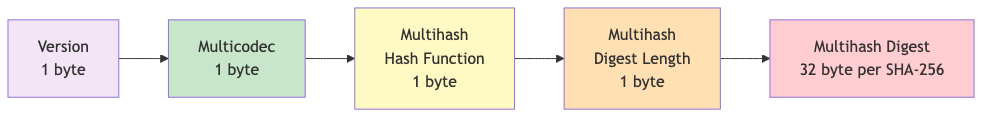
\includegraphics[keepaspectratio,alt={Diagramma Mermaid}]{images/mermaid-lezione-24-ipfs-interplanetary-file-system-02.png}}
\emph{Fig. --- Struttura a byte di un CIDv1 (dag-pb, sha2-256):
versione, multicodec, funzione di hash, lunghezza, digest.}

Il CID completo è quindi un flusso di byte che viene poi raggruppato in
chunk da 5 bit e codificato --- tramite multibase --- in caratteri
Base32 (o altra base). Il carattere di prefisso della stringa finale
identifica la base usata, completando il quadro auto-descrittivo.

\begin{calloutnote}{Perché 5 bit per Base32}

Base32 usa 32 simboli distinti, cioè \(2^5\). Ogni gruppo di 5 bit del
flusso binario diventa un carattere dell'alfabeto Base32. Si noti che i
confini dei campi originari (versione, multicodec, ecc.) \textbf{non}
sono allineati ai 5 bit: nella stringa Base32 finale la struttura a byte
non è più visibile, si può recuperare solo dopo aver decodificato.

\end{calloutnote}

\begin{center}\rule{0.5\linewidth}{0.5pt}\end{center}

\section{IPLD e il Merkle DAG}\label{ipld-e-il-merkle-dag}

Fin qui abbiamo parlato di file singoli. Ma IPFS deve gestire anche
strutture più complesse --- directory, collezioni di blocchi, versioni
successive di uno stesso documento --- e lo fa attraverso un livello
chiamato \textbf{IPLD (InterPlanetary Linked Data)}, il modello dati di
IPFS.

\begin{calloutdefinition}{IPLD e Merkle DAG}

IPLD trasforma tutti i dati in un \textbf{grafo di nodi collegati da
CID}. Ogni pezzo di dato è un nodo; i nodi sono connessi da \emph{link},
dove un link è semplicemente il CID del nodo di destinazione. L'insieme
forma un \textbf{Merkle DAG (Directed Acyclic Graph)}: un grafo
orientato aciclico in cui ogni nodo contiene, all'interno dei propri
dati, i digest dei nodi figli.

\end{calloutdefinition}

L'aggettivo ``Merkle'' viene dalle classiche strutture crittografiche di
Ralph Merkle: \textbf{il contenuto di cui si calcola l'hash contiene i
digest di altri contenuti}, quindi ogni nodo autentica ricorsivamente
tutti i suoi discendenti. L'hash della radice è sufficiente per
verificare l'integrità dell'intera struttura.

\subsection{Come funziona in concreto}\label{come-funziona-in-concreto}

Quando aggiungi un file a IPFS, il sistema lo divide in \textbf{chunk}
(blocchi di dimensione fissa o variabile). Per ogni chunk calcola un
digest e crea un CID. Poi costruisce un nodo ``indice'' che contiene i
CID dei chunk in ordine, e ne calcola a sua volta il CID: questo è il
\textbf{base CID} del file.

\pandocbounded{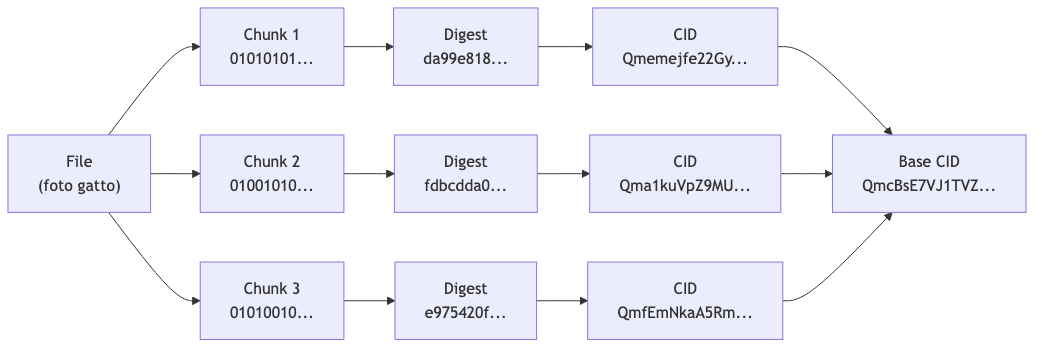
\includegraphics[keepaspectratio,alt={Diagramma Mermaid}]{images/mermaid-lezione-24-ipfs-interplanetary-file-system-03.png}}
\emph{Fig. --- Costruzione del Merkle DAG di un file: chunking, hashing,
generazione dei CID dei figli e del CID radice.}

\subsection{Deduplicazione automatica}\label{deduplicazione-automatica}

Una conseguenza bellissima di questa struttura è la
\textbf{deduplicazione}: lo stesso contenuto è memorizzato \textbf{una
sola volta} nell'intera rete. Se due foto condividono gli stessi chunk
--- perché sono simili, perché hanno la stessa intestazione, perché
qualcuno ha modificato solo una piccola parte dell'immagine --- la parte
comune ha lo stesso CID in entrambi i file, quindi non viene duplicata.

L'esempio limite è evocativo: immagina che ogni lettera dell'alfabeto
abbia il suo CID e sia memorizzata una sola volta nel sistema. Un intero
libro potrebbe essere rappresentato \emph{componendo i CID delle
lettere} --- ovviamente in pratica si lavora a grana più grossa, ma
l'idea è quella.

Il diagramma seguente mostra concretamente come IPLD organizza i dati in
un Merkle DAG, evidenziando il caso in cui un nodo (qui \texttt{CID\_D})
è \textbf{condiviso} fra più genitori --- ed è proprio questo che rende
la struttura un DAG e non un semplice albero.

\pandocbounded{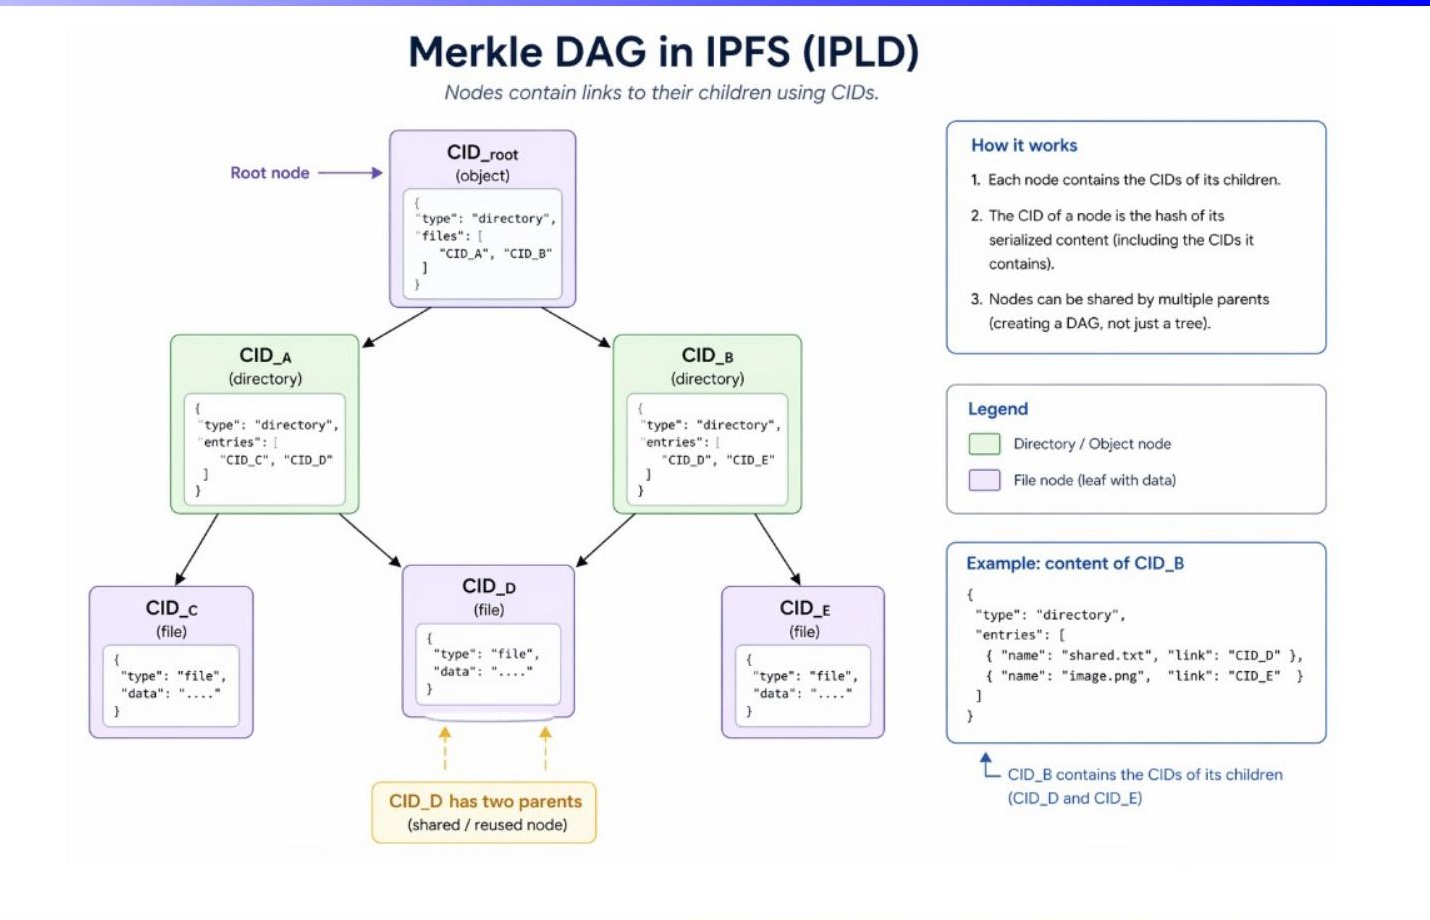
\includegraphics[keepaspectratio,alt={Merkle DAG in IPFS (IPLD) --- nodi che contengono link ai figli tramite CID, con un nodo condiviso fra due genitori}]{images/lezione-24-ipfs-interplanetary-file-system-img-01.jpg}}
\emph{Fig. --- Merkle DAG in IPFS (IPLD). \texttt{CID\_root} contiene i
CID dei figli \texttt{CID\_A} e \texttt{CID\_B} (entrambe directory). Il
file \texttt{CID\_D} è referenziato sia da \texttt{CID\_A} sia da
\texttt{CID\_B}: essendo identificato dall'hash del suo contenuto, viene
memorizzato una sola volta ma puntato da più genitori. A destra,
l'esempio del payload serializzato di \texttt{CID\_B}, che elenca i suoi
figli come coppie \texttt{(name,\ link)}.}

\subsection{Proprietà del Merkle DAG}\label{proprietuxe0-del-merkle-dag}

La struttura ha tre proprietà fondamentali che conviene tenere a mente.

\textbf{Il CID di un nodo dipende dai CID di tutti i suoi discendenti.}
Se fotoritocchi anche un solo pixel di un'immagine contenuta in una
directory, il CID del chunk modificato cambia; di conseguenza cambia il
CID del nodo che lo contiene; poi cambia il CID della directory; e così
via fino alla radice. La modifica \textbf{si propaga verso gli
antenati}, mai verso i fratelli.

\textbf{La costruzione avviene sempre dal basso verso l'alto.} Non si
può creare un nodo padre finché i CID dei figli non sono noti. Questa è
anche la ragione strutturale per cui il DAG non può contenere cicli:
sarebbe una dipendenza circolare dei CID.

\textbf{Una modifica in un ramo non tocca gli altri rami.} Se cambi un
file in \texttt{dir/foto/gatto.jpg}, i CID di tutti i file dentro
\texttt{dir/foto/} vengono ricalcolati solo per il ramo interessato; gli
altri file della directory mantengono invariato il loro CID. È la stessa
proprietà che in Git permette di identificare in modo compatto un commit
e di verificare rapidamente l'identità di due sottocartelle.

\begin{callouttip}{Verifica di due directory}

Hai fatto una copia di backup di una directory durante un lavoro di
editing, mesi fa. Oggi ritrovi le due copie e vuoi sapere se hanno lo
stesso contenuto. Invece di confrontare file per file, calcoli il Merkle
DAG di ciascuna: se i CID delle radici coincidono, le due directory sono
\emph{identiche} bit per bit --- puoi cancellare una delle due in tutta
sicurezza e liberare spazio. È lo stesso principio con cui Git confronta
due commit.

\end{callouttip}

\subsection{Ogni nodo può essere
radice}\label{ogni-nodo-puuxf2-essere-radice}

Il Merkle DAG è \textbf{ricorsivo}: ogni sottografo è a sua volta un DAG
completo, con una sua radice (il suo nodo di partenza) e un suo CID.
Questo apre possibilità espressive molto potenti.

\begin{callouttip}{DAG come strutture componibili}

\begin{itemize}
\tightlist
\item
  Puoi \textbf{condividere un sottografo} semplicemente inviando il CID
  della sua radice --- il destinatario non ha bisogno del contesto del
  grafo più grande.
\item
  Puoi \textbf{incorporare lo stesso sottografo in DAG diversi}: il CID
  del sottografo dipende solo dai suoi discendenti, non dai suoi
  antenati. Lo stesso file, lo stesso chunk, la stessa directory possono
  apparire in posizioni diverse di DAG diversi senza essere duplicati.
\end{itemize}

\end{callouttip}

Questa proprietà è la base strutturale su cui IPFS costruisce file
system versionati, blockchain e, più in generale, qualunque sistema che
abbia bisogno di memorizzare dati autenticati, componibili e
condivisibili.

\begin{center}\rule{0.5\linewidth}{0.5pt}\end{center}

\section{Il livello di rete: libp2p}\label{il-livello-di-rete-libp2p}

Passiamo dalla struttura dei dati al modo in cui i nodi si parlano. Il
livello di rete di IPFS è implementato da \textbf{libp2p}, una libreria
modulare nata come sotto-progetto di IPFS e oggi usata da molti altri
progetti peer-to-peer (tra cui Ethereum 2.0, Polkadot, Filecoin).

Libp2p si occupa di tutto ciò che serve per mettere in comunicazione due
nodi senza fare assunzioni sulla rete sottostante. Le funzionalità
principali sono:

{\def\LTcaptype{none} % do not increment counter
\begin{longtable}[]{@{}
  >{\raggedright\arraybackslash}p{(\linewidth - 2\tabcolsep) * \real{0.5000}}
  >{\raggedright\arraybackslash}p{(\linewidth - 2\tabcolsep) * \real{0.5000}}@{}}
\toprule\noalign{}
\begin{minipage}[b]{\linewidth}\raggedright
Funzionalità
\end{minipage} & \begin{minipage}[b]{\linewidth}\raggedright
Cosa fa
\end{minipage} \\
\midrule\noalign{}
\endhead
\bottomrule\noalign{}
\endlastfoot
\textbf{Peer discovery} & trovare altri nodi tramite Kademlia DHT, mDNS,
bootstrap node \\
\textbf{Transport abstraction} & supportare TCP, QUIC, WebSocket, WebRTC
in modo trasparente \\
\textbf{Connection establishment} & aprire connessioni anche attraverso
NAT e firewall (hole punching, relay) \\
\textbf{Secure communication} & cifratura e autenticazione (Noise, TLS)
--- i peer hanno identità crittografiche \\
\textbf{Stream multiplexing} & più stream logici sulla stessa
connessione (come HTTP/2) \\
\textbf{Protocol handling} & supporto a protocolli custom
(Request/Response, PubSub) \\
\textbf{Peer routing} e \textbf{Content routing} & trovare peer e
contenuti \\
\textbf{PubSub messaging} & canali di publish/subscribe (es.
Gossipsub) \\
\textbf{NAT traversal \& relay} & raggiungere peer dietro NAT \\
\textbf{Peer identity} & ogni nodo ha un PeerId crittografico \\
\end{longtable}
}

\subsection{PeerId e multiaddress}\label{peerid-e-multiaddress}

Ogni peer possiede una coppia di chiavi \textbf{(pubblica, privata)}. Il
\textbf{PeerId} è l'hash crittografico della chiave pubblica --- cioè un
CID, coerentemente con la filosofia content-based di IPFS. La coppia di
chiavi permette poi di stabilire canali sicuri e autenticati tra peer.

\begin{calloutdefinition}{Multiaddress}

Un \textbf{multiaddress} è un indirizzo di rete \textbf{self-describing}
che contiene tutte le informazioni necessarie per raggiungere un peer:
protocollo di rete, indirizzo, porta, protocollo applicativo, PeerId.

\end{calloutdefinition}

Un esempio concreto:

\begin{verbatim}
/ip4/127.0.0.1/tcp/4001/p2p/12D3KooWJ...
\end{verbatim}

Letto da sinistra a destra: ``usa IPv4, indirizzo 127.0.0.1, protocollo
TCP, porta 4001, protocollo p2p, PeerId 12D3KooWJ\ldots{}''. La
struttura è componibile: si può sostituire \texttt{ip4} con
\texttt{ip6}, \texttt{tcp} con \texttt{udp}/\texttt{quic}, aggiungere
\texttt{wss} per WebSocket sicuri, o wrappare tutto in un relay. Ogni
componente ha un codice di protocollo (varint) che lo identifica e
alcuni hanno una lunghezza/byte value associati.

\begin{callouttip}{Perché il multiaddress è così flessibile}

\begin{itemize}
\tightlist
\item
  \textbf{Self-describing}: contiene tutti i protocolli e gli indirizzi
  necessari.
\item
  \textbf{Composable}: è fatto di componenti di protocollo
  concatenabili.
\item
  \textbf{Transport agnostic}: funziona con qualsiasi protocollo di
  rete.
\item
  \textbf{Extensible}: aggiungere nuovi protocolli è facile.
\end{itemize}

\end{callouttip}

Esempi tipici: \texttt{/ip4/127.0.0.1/tcp/4001/p2p/12D3Koo...} per una
connessione TCP locale, \texttt{/ip4/203.0.113.10/tcp/4001/p2p/12D3...}
per TCP pubblico, \texttt{/dns4/example.com/tcp/443/wss/p2p/12D3...} per
WebSocket su HTTPS,
\texttt{/ip6/2001:db8::1/udp/443/quic-v1/p2p/12D3...} per QUIC su IPv6.

\begin{center}\rule{0.5\linewidth}{0.5pt}\end{center}

\section{Il livello di routing: la
DHT}\label{il-livello-di-routing-la-dht}

Quando richiedi un contenuto a partire dal suo CID, IPFS deve risolvere
una domanda precisa: \textbf{quali peer hanno questo contenuto?} È
compito del livello di \textbf{routing}, implementato tramite una
\textbf{DHT (Distributed Hash Table)}.

\begin{calloutwarning}{Cosa fa (e cosa non fa) la DHT di IPFS}

La DHT di IPFS \textbf{non memorizza i dati}. Memorizza soltanto una
mappa
\texttt{CID\ →\ lista\ di\ PeerId\ che\ hanno\ dichiarato\ di\ averlo}.
Quando un nodo pubblica un contenuto, annuncia alla DHT ``io ho questo
CID''; la DHT registra il mapping. Quando qualcuno cerca il CID, la DHT
risponde ``prova a chiedere a questi peer''. Il trasferimento vero e
proprio avviene \textbf{peer-to-peer direttamente}, bypassando la DHT.

\end{calloutwarning}

Inoltre la DHT serve anche per la \textbf{peer discovery}: se hai un
PeerId e vuoi sapere come raggiungerlo, la DHT può restituirti il suo
multiaddress.

Il problema che risolve è concreto: tu hai un CID
\texttt{bafybeigdyrzt...} ma non sai né chi ha il dato né da dove
scaricarlo. La DHT fa da ``elenco telefonico'' decentralizzato: usa
l'hash del file come chiave e restituisce le \emph{locations} (i peer)
del file.

\subsection{Miglioramenti rispetto a
Kademlia}\label{miglioramenti-rispetto-a-kademlia}

La DHT vanilla di Kademlia non basta per un sistema in produzione: IPFS
adotta una serie di miglioramenti presi da due filoni di ricerca.

\begin{calloutnote}{Estensioni adottate}

\begin{itemize}
\tightlist
\item
  \textbf{S/Kademlia} --- migliora la \textbf{sicurezza} contro attacchi
  Sybil ed eclipse: invece di affidarsi a un singolo percorso di
  routing, cerca i nodi attraverso percorsi disgiunti e verifica
  l'identità dei peer con primitive crittografiche.
\item
  \textbf{Coral sloppy DHT} --- migliora la \textbf{performance} con una
  struttura gerarchica che permette di trovare repliche ``vicine''
  (geograficamente o in termini di latenza), evitando di contattare
  sempre lo stesso nodo logicamente responsabile di una chiave.
\end{itemize}

\end{calloutnote}

\begin{center}\rule{0.5\linewidth}{0.5pt}\end{center}

\section{Il livello di scambio:
Bitswap}\label{il-livello-di-scambio-bitswap}

Una volta che la DHT ti ha detto ``questi peer dovrebbero avere il
contenuto'', serve un protocollo per \textbf{scambiare effettivamente i
blocchi}. È il compito di \textbf{Bitswap}, il livello di exchange di
IPFS.

\subsection{Perché non basta la DHT}\label{perchuxe9-non-basta-la-dht}

La DHT ti dice ``questo peer \textbf{ha annunciato} di avere il CID'',
ma non garantisce che ce l'abbia \emph{in questo momento}. Tra il tempo
in cui un peer pubblica l'annuncio e il tempo in cui un client cerca il
contenuto possono succedere molte cose: il peer può essere andato
offline, il blocco può essere stato rimosso (unpin, garbage collection),
il peer può non rispondere per problemi di rete. L'informazione della
DHT può essere \textbf{obsoleta}.

\begin{calloutnote}{Division of labor}

\begin{itemize}
\tightlist
\item
  \textbf{DHT} risponde alla domanda ``\emph{chi potrebbe avere il
  CID?}'' --- è un elenco, non una garanzia.
\item
  \textbf{Bitswap} risponde alla domanda ``\emph{chi effettivamente me
  lo dà adesso?}'' --- è il protocollo real-time che scarica i blocchi.
\end{itemize}

\end{calloutnote}

\subsection{Bitswap vs BitTorrent}\label{bitswap-vs-bittorrent}

Bitswap è ispirato a BitTorrent ma non coincide con esso. La differenza
fondamentale è architetturale:

{\def\LTcaptype{none} % do not increment counter
\begin{longtable}[]{@{}
  >{\raggedright\arraybackslash}p{(\linewidth - 2\tabcolsep) * \real{0.5000}}
  >{\raggedright\arraybackslash}p{(\linewidth - 2\tabcolsep) * \real{0.5000}}@{}}
\toprule\noalign{}
\begin{minipage}[b]{\linewidth}\raggedright
BitTorrent
\end{minipage} & \begin{minipage}[b]{\linewidth}\raggedright
Bitswap (IPFS)
\end{minipage} \\
\midrule\noalign{}
\endhead
\bottomrule\noalign{}
\endlastfoot
uno \textbf{swarm separato} per ogni file & un \textbf{unico swarm
globale} per tutti i contenuti condivisi dagli utenti \\
il peer cerca chi ha quel file specifico & il peer partecipa a un unico
mercato di blocchi in cui tutti domandano e offrono CID qualsiasi \\
file diviso in pezzi & tutto è diviso in \textbf{blocchi}, la più
piccola unità di dato trasferibile \\
\end{longtable}
}

Il white paper originale introduce anche una \textbf{strategia di
bartering} di base per lo scambio (tu mi dai blocchi, io te ne do in
cambio), che nel progetto \textbf{Filecoin} viene poi estesa con una
criptovaluta vera e propria.

\subsection{Come funziona un trasferimento
Bitswap}\label{come-funziona-un-trasferimento-bitswap}

Il protocollo ruota attorno a quattro tipi di messaggio: \textbf{WANT}
(voglio questo CID), \textbf{HAVE} (ho questo CID), \textbf{REQUEST}
(mandami il blocco), \textbf{BLOCK} (ecco il blocco).

\pandocbounded{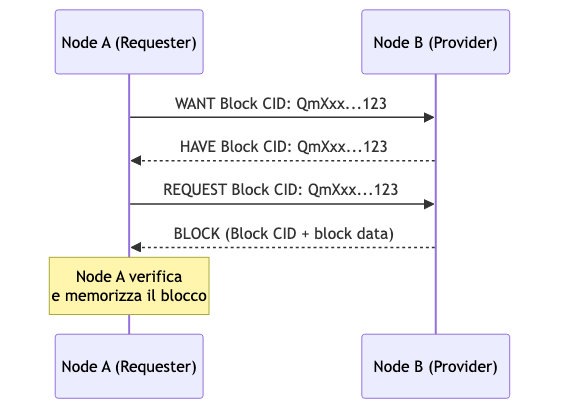
\includegraphics[keepaspectratio,alt={Diagramma Mermaid}]{images/mermaid-lezione-24-ipfs-interplanetary-file-system-04.png}}
\emph{Fig. --- Scambio Bitswap: il nodo A chiede un blocco, il nodo B
conferma di averlo, A richiede i dati e B li invia. A verifica
l'integrità ricalcolando il CID.}

\textbf{A cosa serve HAVE?} Fornisce una \textbf{conferma in tempo
reale}: la DHT dice ``potrebbe avere'', HAVE dice ``ce l'ho
\emph{adesso}''. È un messaggio \textbf{opzionale}: un peer può
rispondere direttamente con il blocco
(\texttt{WANT\ →\ REQUEST\ →\ BLOCK}), saltando la conferma intermedia.
Bitswap è \textbf{best effort}: se un peer non risponde, il richiedente
può provare con altri peer --- nessuna garanzia di consegna da un
singolo fornitore, ma alta probabilità grazie alla molteplicità.

\begin{callouttip}{Punti chiave di Bitswap}

\begin{itemize}
\tightlist
\item
  I blocchi sono identificati dal loro CID (content ID).
\item
  Bitswap è \textbf{demand-driven} ed efficiente: nulla viene trasferito
  se nessuno lo richiede.
\item
  \textbf{Più provider} possono rispondere allo stesso WANT in
  parallelo: il richiedente scarica dal più veloce.
\item
  La verifica avviene \textbf{lato ricevente} ricalcolando l'hash dei
  blocchi ricevuti.
\end{itemize}

\end{callouttip}

\begin{center}\rule{0.5\linewidth}{0.5pt}\end{center}

\section{Disponibilità dei file: il problema della
persistenza}\label{disponibilituxe0-dei-file-il-problema-della-persistenza}

Il modello peer-to-peer di IPFS ha un vantaggio enorme --- la
replicazione naturale dei contenuti popolari --- ma porta con sé un
problema di disponibilità. Dove sono memorizzati i file in IPFS? Ogni
nodo mantiene una \textbf{cache} dei file che ha scaricato o condiviso;
rimane online fintanto che ha interesse a esserlo e aiuta a distribuire
se altri utenti lo richiedono. È un modello simile a uno swarm
BitTorrent, con la differenza che \textbf{esiste un solo swarm per tutti
i contenuti} anziché uno swarm per file.

\begin{calloutwarning}{Cosa succede se tutti i nodi che ospitano un file vanno offline?}

Il file diventa \textbf{irraggiungibile}. Il CID resta valido in
astratto (è una proprietà matematica del contenuto), ma non c'è nessuno
sulla rete che possa servire i blocchi corrispondenti. Questo è il
problema di \textbf{persistenza dei dati} in IPFS.

\end{calloutwarning}

Tre strategie di mitigazione sono possibili.

\begin{enumerate}
\def\labelenumi{\arabic{enumi}.}
\tightlist
\item
  \textbf{Pinning services} --- servizi centralizzati che mantengono
  sempre attivi i contenuti di interesse.
\item
  \textbf{Incentivazione economica} --- pagare i nodi per tenere online
  certi file (la soluzione di Filecoin).
\item
  \textbf{Distribuzione proattiva} --- replicare attivamente i file per
  garantire un numero minimo di copie nella rete.
\end{enumerate}

\subsection{Pinning services: Pinata}\label{pinning-services-pinata}

\textbf{Pinata} è l'esempio più noto di pinning service centralizzato.
Gestisce la propria infrastruttura, pinna i dati dei clienti e
garantisce uptime.

\begin{calloutnote}{Come funziona Pinata}

Pinata esegue i propri nodi IPFS e ``pinna'' (fissa) i contenuti che i
clienti caricano: significa che quei nodi non cancelleranno mai il
blocco né lo rimuoveranno dalla cache. Risultato: il CID resta sempre
servibile. L'interfaccia è semplice: \emph{upload → ottieni CID → il
dato resta disponibile}. È essenzialmente uno ``storage cloud per
IPFS''.

\end{calloutnote}

Un aspetto importante: siccome il CID identifica il \emph{contenuto} e
non il \emph{server}, lo stesso CID può essere pinnato
\textbf{contemporaneamente} su Pinata, sul tuo nodo locale, e su altri
peer. Non c'è un ``vero proprietario'' del dato --- c'è solo un insieme
di nodi che lo servono, e basta che uno sia raggiungibile perché il file
sia accessibile.

\subsection{Filecoin: incentivare lo storage con una
criptovaluta}\label{filecoin-incentivare-lo-storage-con-una-criptovaluta}

Filecoin prende questa idea e la decentralizza: invece di un pinning
service centralizzato, costruisce \textbf{un mercato decentralizzato per
lo storage} sopra IPFS.

\begin{calloutdefinition}{Filecoin}

Filecoin è un layer costruito sopra IPFS che trasforma lo storage in un
bene scambiabile sul mercato. I nodi che hanno spazio libero sul disco
possono affittarlo ad altri utenti e guadagnare in cambio un token,
\textbf{FIL}. I clienti pagano in FIL per memorizzare i loro dati sulla
rete.

\end{calloutdefinition}

L'idea economica è potente: c'è una quantità enorme di spazio storage
inutilizzato sui computer del mondo, e al tempo stesso una domanda
crescente di cloud storage. Filecoin connette domanda e offerta in un
mercato competitivo.

Vantaggi rispetto alle alternative centralizzate (Pinata, Google Drive,
Dropbox):

\begin{itemize}
\tightlist
\item
  \textbf{Prezzi più equi} --- il mercato competitivo tende a pressare
  al ribasso i prezzi rispetto a quelli delle infrastrutture
  centralizzate.
\item
  \textbf{Efficienza di utilizzo} --- invece di costruire nuovo storage,
  si sfrutta quello esistente e sottoutilizzato.
\item
  \textbf{Decentralizzazione} --- nessun punto di fallimento unico,
  nessun singolo fornitore che può chiudere l'account.
\end{itemize}

Il token FIL viene usato dai client per pagare lo storage, e dai
\emph{miner} come ricompensa per i task che svolgono: memorizzare i
dati, dimostrare crittograficamente di continuare a memorizzarli nel
tempo, proteggere la rete, validare le transazioni.

\begin{center}\rule{0.5\linewidth}{0.5pt}\end{center}

\section{NFT e IPFS}\label{nft-e-ipfs}

Un uso concreto e molto diffuso di IPFS è lo storage dei metadata e
degli asset degli \textbf{NFT (Non-Fungible Token)}. Un NFT su Ethereum
non contiene di solito l'immagine o il file multimediale vero e proprio
(sarebbe proibitivamente costoso in gas): contiene un \textbf{puntatore}
a dove quel contenuto è memorizzato.

\begin{calloutwarning}{Il rischio dei puntatori HTTP}

Se il puntatore è un URL HTTP
(\texttt{https://mysite.com/nft-image.jpg}), il NFT è tanto permanente
quanto il dominio e il server. Se il sito chiude, l'immagine sparisce
--- e con essa tutto ciò che l'NFT ``rappresenta''. Storie di NFT che
hanno perso il loro contenuto sono frequenti proprio per questa ragione.

\end{calloutwarning}

La soluzione è usare un \textbf{CID IPFS} come puntatore. Il CID è
immutabile e content-addressed: anche se un nodo specifico va offline,
finché il contenuto esiste da qualche parte nella rete IPFS (tipicamente
pinnato su un servizio come Pinata o su Filecoin), il NFT continua a
puntare correttamente al contenuto originale. I marketplace NFT
(OpenSea, Rarible, ecc.) leggono il CID dal metadata del token e
risolvono il contenuto tramite IPFS gateway.

\begin{callouttip}{Perché IPFS è naturale per gli NFT}

Il CID \textbf{è} un'impronta digitale crittografica del contenuto. Se
un giorno qualcuno sostituisse l'immagine con un'altra, il CID sarebbe
diverso: non può silenziosamente cambiare a cosa punta un NFT.
L'immutabilità dell'NFT sulla blockchain si estende, tramite il CID,
all'immutabilità del contenuto puntato.

\end{callouttip}

\begin{center}\rule{0.5\linewidth}{0.5pt}\end{center}

\section{Sintesi}\label{sintesi}

\begin{calloutnote}{Riepilogo della lezione}

IPFS è un protocollo P2P \textbf{content-based} che sostituisce
l'indirizzamento HTTP basato sulla location con identificatori
crittografici (\textbf{CID}) derivati dal contenuto stesso. Lo stack si
articola su tre blocchi logici: \textbf{trasporto} (libp2p per la rete,
DHT per il routing, Bitswap per lo scambio), \textbf{definizione} (IPLD
con Merkle DAG per la strutturazione dei dati, IPNS per il naming),
\textbf{applicazioni}. Il progetto \textbf{Multiformat} (multihash,
multibase, multicodec, multiaddr) rende tutti i valori auto-descrittivi,
permettendo al protocollo di evolvere senza rompere il software
esistente. Il \textbf{Merkle DAG} garantisce deduplicazione automatica,
verifica crittografica end-to-end e versionamento naturale. La
\textbf{persistenza} dei dati è un problema aperto, mitigato da servizi
di pinning centralizzati (\textbf{Pinata}) o dal mercato decentralizzato
di \textbf{Filecoin}, che incentiva lo storage con una criptovaluta.

\end{calloutnote}

\newpage

\chapter{Ethereum Consensus: Proof of
Stake}\label{ethereum-consensus-proof-of-stake}

\section{Il Problema del Consenso
Distribuito}\label{il-problema-del-consenso-distribuito}

Il consenso distribuito nasce da una sfida fondamentale: costruire un
sistema affidabile su un'infrastruttura inaffidabile. Nell'ecosistema
blockchain, ``inaffidabile'' significa che i nodi comunicano su Internet
--- con banda limitata, alta latenza, perdita di pacchetti --- e possono
comportarsi in modo arbitrariamente difettoso: possono semplicemente
andare offline, seguire una versione diversa del protocollo, o tentare
attivamente di ingannare altri nodi pubblicando messaggi contraddittori.
L'obiettivo del consenso è fare in modo che decine di migliaia di nodi
indipendenti, sparsi per il mondo, procedano in modo completamente
sincronizzato.

\subsection{Il Problema dei Generali
Bizantini}\label{il-problema-dei-generali-bizantini}

Il modello teorico di riferimento è il \textbf{Byzantine Generals
Problem} (problema dei generali bizantini). Nell'analogia classica, un
esercito circonda una città e i generali devono decidere unanimemente se
attaccare o ritirarsi: possono comunicare solo tramite messaggeri, e
alcuni generali potrebbero essere traditori.

I ``traditori'' esibiscono un \textbf{comportamento bizantino}: possono
ritardare o riordinare messaggi, mentire, inviare messaggi
contraddittori a destinatari diversi, o non rispondere affatto. Il
requisito del consenso è che tutti i generali leali decidano lo stesso
piano d'azione, e che nessun numero di traditori al di sotto di una
certa soglia possa portarli ad adottare piani contraddittori.

\begin{center}\rule{0.5\linewidth}{0.5pt}\end{center}

\section{Safety e Liveness}\label{safety-e-liveness}

Due proprietà fondamentali definiscono la qualità di un protocollo di
consenso.

\begin{calloutdefinition}{Safety — “Non accade mai nulla di brutto”}

Il sistema non raggiunge mai uno stato scorretto o inconsistente. Nel
contesto della blockchain: nessun nodo onesto decide valori diversi
sullo stesso blocco. La safety corrisponde all'assenza di conflitti e
fork permanenti.

\end{calloutdefinition}

\begin{calloutdefinition}{Liveness — “Prima o poi accade qualcosa di buono”}

Il sistema non si blocca indefinitamente. Nella blockchain: le
transazioni vengono eventualmente incluse in un blocco, e nuovi blocchi
vengono prodotti continuamente. La violazione della liveness è una
situazione di stallo.

\end{calloutdefinition}

Il \textbf{Nakamoto Consensus} di Bitcoin sceglie deliberatamente di
privilegiare la liveness rispetto alla safety: la catena continua sempre
a crescere (always available), ma accetta inconsistenze temporanee sotto
forma di fork, che vengono risolti applicando la regola della catena più
lunga. La safety in Bitcoin è quindi \emph{probabilistica}: non c'è
finality assoluta, ma più conferme accumulate, più è improbabile
un'inversione di catena.

\begin{calloutwarning}{CAP Theorem}

Il teorema CAP (Consistency, Availability, Partition Tolerance) afferma
che, in presenza di una partizione di rete, un sistema distribuito deve
scegliere tra consistenza (nessun nodo vede dati obsoleti) e
disponibilità (ogni nodo risponde sempre). Non è possibile garantire
entrambe simultaneamente.

\end{calloutwarning}

\begin{center}\rule{0.5\linewidth}{0.5pt}\end{center}

\section{Dalla Proof of Work alla Proof of
Stake}\label{dalla-proof-of-work-alla-proof-of-stake}

\subsection{Limiti del Nakamoto
Consensus}\label{limiti-del-nakamoto-consensus}

Il mining Bitcoin ha costi enormi: consuma quantità sproporzionate di
energia, e i mining pool controllano porzioni crescenti della catena,
erodendo la decentralizzazione. Le alternative al PoW includono:

\begin{itemize}
\tightlist
\item
  \textbf{Proof of Stake} (Ethereum 2.0, Algorand, Cardano, Solana)
\item
  \textbf{Delegated Proof of Stake} (Steemit, EOS)
\item
  \textbf{Byzantine Consensus} (Hyperledger)
\end{itemize}

\subsection{La Timeline di Ethereum
2.0}\label{la-timeline-di-ethereum-2.0}

\pandocbounded{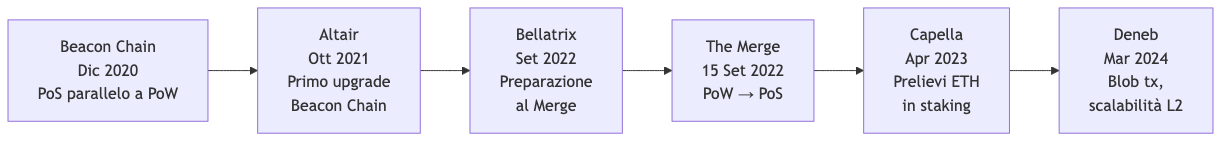
\includegraphics[keepaspectratio,alt={Diagramma Mermaid}]{images/mermaid-lezione-25-ethereum-consensus-proof-of-stake-01.png}}
\emph{Fig. --- Timeline degli upgrade del Consensus Layer di Ethereum
2.0, da Beacon Chain a Deneb.}

La \textbf{Beacon Chain} è stata una rete PoS completamente indipendente
che ha funzionato in parallelo alla Mainnet Ethereum per quasi due anni.
Il suo scopo era supportare la transizione senza interrompere il
servizio. \textbf{The Merge} del 15 settembre 2022 ha unito la Execution
Layer (Mainnet) con la Consensus Layer (Beacon Chain), completando il
passaggio da PoW a PoS.

\begin{center}\rule{0.5\linewidth}{0.5pt}\end{center}

\section{Gasper: LMD GHOST + Casper
FFG}\label{gasper-lmd-ghost-casper-ffg}

Il protocollo di consenso di Ethereum PoS è detto \textbf{Gasper} e
combina due meccanismi distinti con ruoli complementari:

\begin{calloutdefinition}{Gasper}

Gasper = \textbf{LMD GHOST} (fork choice, liveness) + \textbf{Casper
FFG} (finality gadget, safety). LMD GHOST sceglie la testa della catena
in presenza di fork; Casper FFG aggiunge la finalità ai checkpoint,
rendendo certi blocchi irrevocabili.

\end{calloutdefinition}

Questa architettura riflette la posizione di Ethereum rispetto al
trade-off del CAP theorem: in condizioni normali, offre sia safety che
liveness; in presenza di partizioni di rete, privilegia la liveness (i
nodi continuano a produrre blocchi), ma la finalità può interrompersi.

\begin{callouttip}{Perché non solo un protocollo?}

LMD GHOST da solo garantisce che la catena cresca sempre, ma non
fornisce garanzie di irrevocabilità --- i blocchi possono sempre essere
riorganizzati. Casper FFG da solo richiederebbe una supermajority in
ogni round e si bloccherebbe se troppi validatori fossero offline. La
combinazione bilancia i due estremi.

\end{callouttip}

\begin{center}\rule{0.5\linewidth}{0.5pt}\end{center}

\section{I Validatori}\label{i-validatori}

\subsection{Ruolo e Incentivi}\label{ruolo-e-incentivi}

In Ethereum PoS non esistono miner. Al loro posto operano i
\textbf{validatori} (validators): nodi che bloccano ETH come garanzia e
partecipano al consenso. Ogni validatore svolge due ruoli:

\begin{itemize}
\tightlist
\item
  \textbf{Block proposer} (raramente): viene selezionato per creare un
  nuovo blocco in uno slot specifico, scegliendo e ordinando le
  transazioni pendenti.
\item
  \textbf{Attester} (la maggior parte del tempo): vota sui blocchi
  proposti, confermando quale sia la testa corretta della catena.
\end{itemize}

\subsection{Diventare un Validatore}\label{diventare-un-validatore}

Per diventare validatore è necessario depositare esattamente \textbf{32
ETH} in un apposito \emph{deposit smart contract}. Il deposito ha una
funzione analoga al \textbf{collaterale} in finanza: un asset offerto
come garanzia. Se il validatore si comporta correttamente, guadagna
ricompense; se agisce in modo malevolo o negligente, può essere
\textbf{slashed}, perdendo una porzione dello stake.

\begin{calloutnote}{Perché 32 ETH fissi?}

Un importo fisso permette di trattare ogni validatore in modo uguale nel
calcolo dei voti. Chiunque può verificare che un validatore abbia
depositato la somma corretta consultando il contratto pubblicamente.

\end{calloutnote}

Il sistema è altamente partecipativo: attualmente ci sono circa
\textbf{1 milione} di istanze di validatori attivi, rendendolo
genuinamente democratico.

\subsection{Staking senza 32 ETH}\label{staking-senza-32-eth}

Chi non dispone di 32 ETH può partecipare tramite \textbf{staking pools}
come Lido o Rocket Pool, o exchange centralizzati come Coinbase o
Binance. In uno staking pool, gli ETH vengono aggregati da operatori
professionali; in cambio si riceve un token che accumula le ricompense
dello staking e può essere usato nei servizi DeFi.

\begin{center}\rule{0.5\linewidth}{0.5pt}\end{center}

\section{Slot ed Epoch}\label{slot-ed-epoch}

A differenza del PoW, che è un protocollo asincrono senza relazione con
il tempo reale, il PoS di Ethereum organizza il tempo in unità discrete.

\begin{calloutdefinition}{Slot ed Epoch}

\begin{itemize}
\tightlist
\item
  \textbf{Slot}: finestra temporale di \textbf{12 secondi}, durante la
  quale un comitato di validatori può votare per un beacon block.
\item
  \textbf{Epoch}: sequenza di \textbf{32 slot} = \textbf{6,4 minuti}. In
  un'epoch, ogni validatore attivo ha esattamente un'opportunità di
  partecipare.
\end{itemize}

\end{calloutdefinition}

\pandocbounded{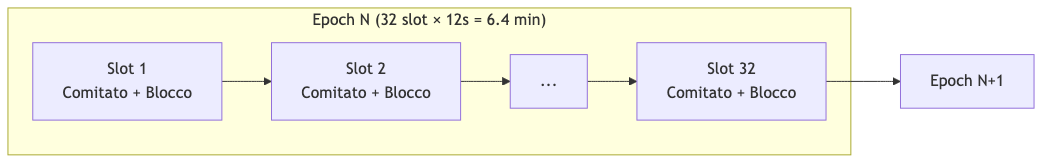
\includegraphics[keepaspectratio,alt={Diagramma Mermaid}]{images/mermaid-lezione-25-ethereum-consensus-proof-of-stake-02.png}}
\emph{Fig. --- Struttura temporale di epoch e slot in Ethereum PoS.}

All'interno di ogni slot si svolgono tre fasi: (1) un singolo validatore
propone un blocco e lo diffonde via gossip; (2) tutti gli altri membri
del comitato emettono il loro voto (attestation); (3) negli ultimi 4
secondi, i voti vengono aggregati e inoltrati al proposer del prossimo
slot.

\begin{center}\rule{0.5\linewidth}{0.5pt}\end{center}

\section{RANDAO: Randomness
Decentralizzata}\label{randao-randomness-decentralizzata}

Ethereum ha bisogno di casualità verificabile per scegliere i block
proposer e assegnare i validatori ai comitati. Non è possibile affidarsi
a un'entità centrale (che potrebbe barare) né a un valore prevedibile
(che potrebbe essere sfruttato). La soluzione è \textbf{RANDAO}: un
protocollo distribuito per generare numeri casuali che nessun singolo
partecipante può controllare.

\subsection{Come Funziona RANDAO}\label{come-funziona-randao}

Il meccanismo segue uno schema commit-reveal in quattro passi:

\pandocbounded{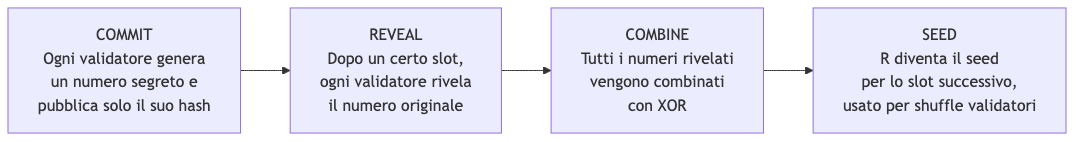
\includegraphics[keepaspectratio,alt={Diagramma Mermaid}]{images/mermaid-lezione-25-ethereum-consensus-proof-of-stake-03.png}}
\emph{Fig. --- Il protocollo RANDAO: dalla generazione del segreto
all'assegnazione dei ruoli.}

Il risultato finale
\(R = n_1 \oplus n_2 \oplus n_3 \oplus \ldots \oplus n_k\) è
imprevedibile perché nessuno conosce tutti i segreti prima della reveal,
è inalterabile dopo il commit, è decentralizzato poiché ogni validatore
contribuisce, ed è verificabile pubblicamente.

L'output RANDAO viene usato come seed per mescolare (\emph{shuffle}) i
validatori e assegnarli a block proposer, comitati, aggregatori e sync
committees, con un anticipo di \textbf{due epoch}.

\begin{center}\rule{0.5\linewidth}{0.5pt}\end{center}

\section{LMD GHOST: Fork Choice}\label{lmd-ghost-fork-choice}

\subsection{Perché si Formano i Fork}\label{perchuxe9-si-formano-i-fork}

In Ethereum, dove i blocchi vengono prodotti ogni 12 secondi, il tempo
di propagazione dei blocchi è dell'ordine di grandezza degli slot
stessi. Non tutti i validatori vedono tutti i blocchi in tempo per
attestarli o costruirci sopra. Il risultato è un albero di blocchi, non
una singola catena.

\subsection{L'Algoritmo LMD GHOST}\label{lalgoritmo-lmd-ghost}

\textbf{LMD GHOST} (\emph{Latest Message Driven Greedy Heaviest-Observed
Sub-Tree}) è la regola di fork choice di Ethereum. L'intuizione centrale
è sostituire la ``catena più lunga'' di Bitcoin con la ``catena con più
stake accumulato'', usando solo il voto più recente di ogni validatore.

\begin{calloutdefinition}{LMD GHOST}

Partendo dall'ultimo blocco finalizzato, l'algoritmo scende l'albero
scegliendo ricorsivamente il ramo con il maggior peso totale. Il peso di
un ramo è la somma del peso di tutti i voti per quel blocco e per tutti
i suoi discendenti. Solo il messaggio più recente (LMD) di ogni
validatore viene considerato.

\end{calloutdefinition}

Il peso di un voto è proporzionale al \textbf{bilancio effettivo} del
validatore al momento del voto: deposito iniziale di 32 ETH, più le
ricompense accumulate, meno le penalità subite. Quindi non conta il
numero di voti, ma la quantità di ETH in staking che li sostiene.

\pandocbounded{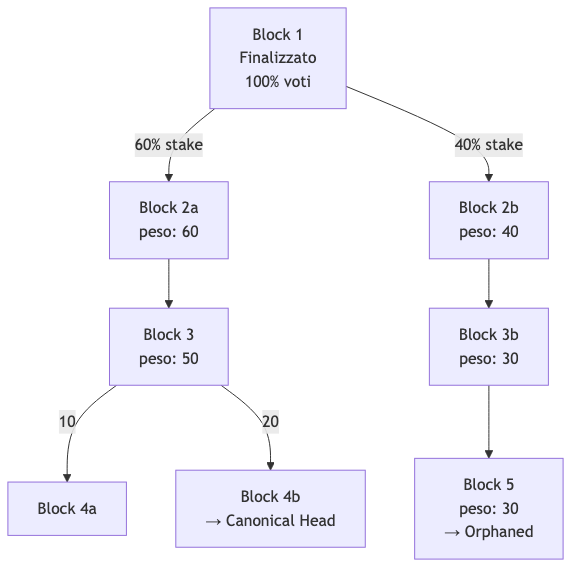
\includegraphics[keepaspectratio,alt={Diagramma Mermaid}]{images/mermaid-lezione-25-ethereum-consensus-proof-of-stake-04.png}}
\emph{Fig. --- LMD GHOST: il ramo superiore (60→50→20) vince sul ramo
inferiore più lungo (40→30→30→30) perché ha più stake accumulato.}

\begin{callouttip}{Intuizione chiave di LMD GHOST}

Un voto per un blocco figlio è implicitamente un voto per tutti i suoi
antenati. Se due figli dello stesso blocco padre ricevono voti da
validatori diversi, entrambi i gruppi stanno confermando il padre. GHOST
sfrutta al massimo tutte le informazioni disponibili, anziché scartarle
come farebbe la longest chain rule.

\end{callouttip}

\begin{center}\rule{0.5\linewidth}{0.5pt}\end{center}

\section{Il Problema del ``Nothing at
Stake''}\label{il-problema-del-nothing-at-stake}

In PoW, produrre un blocco è costoso in termini computazionali: questo
incentiva i miner a concentrare le risorse su un'unica catena. In PoS
naive, creare nuovi blocchi è quasi gratuito, creando il problema del
\textbf{nothing at stake}: un validatore razionale potrebbe votare per
tutte le catene concorrenti contemporaneamente, massimizzando la
probabilità di essere sul lato vincente indipendentemente dall'esito.

Le conseguenze sono severe: più fork perché i validatori attestano tutti
i rami, risorse sprecate su catene orfane, tempi di finalità più lunghi,
e vulnerabilità agli attacchi di double-spending.

\subsection{Lo Slashing come
Soluzione}\label{lo-slashing-come-soluzione}

Ethereum risolve questo problema con il \textbf{slashing}: se un
validatore viene trovato in \emph{equivocazione} (ha firmato due blocchi
diversi per lo stesso slot, o ha violato le regole di Casper FFG), viene
punito con la rimozione di una parte del suo stake e l'espulsione dal
protocollo.

\begin{calloutwarning}{Slashing accidentale}

La maggior parte degli eventi di slashing non è dolosa: è dovuta a
errori operativi come avere due client attivi con la stessa chiave (es.
nodo principale + nodo di backup entrambi ON), configurazioni errate di
Docker/Kubernetes, o failover senza spegnere l'istanza precedente. Un
validatore deve comportarsi come una singola entità.

\end{calloutwarning}

\begin{center}\rule{0.5\linewidth}{0.5pt}\end{center}

\section{Casper FFG: Finality Gadget}\label{casper-ffg-finality-gadget}

\subsection{Il Concetto di Finality}\label{il-concetto-di-finality}

In Bitcoin la finality è probabilistica: più conferme, meno probabile la
reversione, ma mai impossibile. \textbf{Casper FFG} (\emph{Friendly
Finality Gadget}) è un protocollo \emph{meta-consenso} che aggiunge
finality assoluta a un protocollo sottostante. In Ethereum, il
protocollo sottostante è LMD GHOST.

\begin{calloutdefinition}{Casper FFG}

Casper FFG è un overlay su LMD GHOST che opera su scala di epoch (non di
singolo slot). Identifica blocchi speciali chiamati \textbf{checkpoint}
e, tramite un processo di votazione a supermajority, li porta allo stato
di \emph{justified} prima, e infine \emph{finalized}.

\end{calloutdefinition}

\subsection{Checkpoint, Justification e
Finalization}\label{checkpoint-justification-e-finalization}

Il primo blocco di ogni epoch è definito \textbf{checkpoint}. Ogni
validatore produce esattamente un'attestazione per epoch, che contiene
due voti:

\begin{itemize}
\tightlist
\item
  \textbf{SOURCE}: il checkpoint dell'epoch precedente già giustificato
  (``costruisco sulla catena giustificata all'epoch \(e-1\)'')
\item
  \textbf{TARGET}: il checkpoint dell'epoch corrente (``voto per questa
  come testa della catena all'epoch \(e\)'')
\end{itemize}

Il formato di un'attestazione è:

{\def\LTcaptype{none} % do not increment counter
\begin{longtable}[]{@{}ll@{}}
\toprule\noalign{}
Campo & Contenuto \\
\midrule\noalign{}
\endhead
\bottomrule\noalign{}
\endlastfoot
\texttt{slot} & slot 0 dell'epoch \(e\) \\
\texttt{index} & indice del validatore \\
\texttt{source} & checkpoint giustificato dell'epoch \(e-1\) \\
\texttt{target} & checkpoint candidato dell'epoch \(e\) \\
\texttt{signature} & firma BLS del validatore \\
\end{longtable}
}

Quando più di \(2/3\) del totale dello stake (pesato per bilancio
effettivo) vota per lo stesso checkpoint, quel checkpoint diventa
\textbf{justified}. Il checkpoint della fonte (source) del round
precedente diventa a sua volta \textbf{finalized}.

\pandocbounded{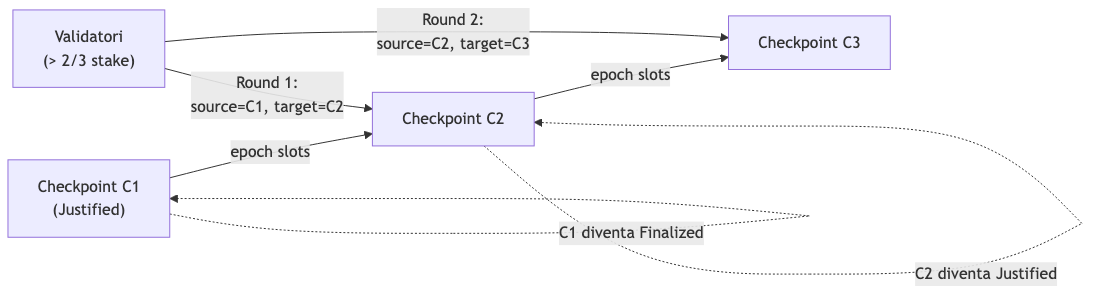
\includegraphics[keepaspectratio,alt={Diagramma Mermaid}]{images/mermaid-lezione-25-ethereum-consensus-proof-of-stake-05.png}}
\emph{Fig. --- Il processo di justification e finalization in Casper
FFG: due supermajority consecutive portano C1 alla finalità.}

\subsection{Perché Due Supermajority Consecutive Garantiscono la
Finalità}\label{perchuxe9-due-supermajority-consecutive-garantiscono-la-finalituxe0}

La prova è elegante e si basa sul principio di inclusione-esclusione.
Siano \(S_1\) e \(S_2\) i due insiemi di validatori che formano la
supermajority in due epoch consecutive. Per definizione:

\[|S_1| \geq \frac{2}{3} N \qquad |S_2| \geq \frac{2}{3} N\]

dove \(N\) è il totale dello stake. Applicando il principio di
inclusione-esclusione, poiché \(|S_1 \cup S_2| \leq N\):

\[|S_1 \cap S_2| = |S_1| + |S_2| - |S_1 \cup S_2| \geq \frac{2}{3}N + \frac{2}{3}N - N = \frac{1}{3}N\]

L'intersezione è quindi almeno \(1/3\) dello stake totale. Qualsiasi
tentativo di costruire una catena conflittuale richiederebbe a questi
validatori di votare in modo inconsistente tra i due epoch, incorrendo
nello slashing. Un attacco che reverta un blocco finalizzato costerebbe
la bruciatura di almeno \(1/3\) di tutto lo stake in Ethereum ---
miliardi di dollari --- rendendo l'attacco economicamente irrazionale.

\begin{calloutnote}{Sintesi del meccanismo di finality}

C1 si finalizza quando: (1) nel Round 1 più di 2/3 dello stake vota C2
con sorgente C1 (C2 diventa justified); (2) nel Round 2 più di 2/3 dello
stake vota C3 con sorgente C2 (C2 diventa justified per la seconda
volta; C1 diventa finalized). La sovrapposizione obbligatoria di almeno
1/3 dello stake tra i due round rende impossibile una revisione senza un
costo economico proibitivo.

\end{calloutnote}

\begin{center}\rule{0.5\linewidth}{0.5pt}\end{center}

\section{Il Traffico di Rete}\label{il-traffico-di-rete}

La scala di Ethereum PoS è senza precedenti nel consenso distribuito: in
384 secondi (un'epoch), oltre \textbf{500.000 messaggi} devono essere
propagati rispettando vincoli temporali rigidi. Nessun altro protocollo
di consenso è stato progettato per un numero simile di partecipanti
attivi.

Per contenere il traffico, Ethereum usa due meccanismi: -
\textbf{Message aggregation}: i comitati sono suddivisi in sottoreti; un
validatore aggregatore raccoglie le firme di tutti i membri e le combina
in una sola usando firme \textbf{BLS} (\emph{Boneh-Lynn-Shacham}), che
consentono di aggregare \(n\) firme in una singola firma verificabile. -
\textbf{Node aggregators}: ruoli specializzati all'interno di ogni
comitato.

\begin{center}\rule{0.5\linewidth}{0.5pt}\end{center}

\section{Ricompense e Penalità}\label{ricompense-e-penalituxe0}

Il comportamento dei validatori è regolato da un sistema di incentivi
economici:

{\def\LTcaptype{none} % do not increment counter
\begin{longtable}[]{@{}
  >{\raggedright\arraybackslash}p{(\linewidth - 2\tabcolsep) * \real{0.5000}}
  >{\raggedright\arraybackslash}p{(\linewidth - 2\tabcolsep) * \real{0.5000}}@{}}
\toprule\noalign{}
\begin{minipage}[b]{\linewidth}\raggedright
Comportamento
\end{minipage} & \begin{minipage}[b]{\linewidth}\raggedright
Conseguenza
\end{minipage} \\
\midrule\noalign{}
\endhead
\bottomrule\noalign{}
\endlastfoot
Attestazione corretta e tempestiva & Micro-ricompensa proporzionale al
bilancio \\
Attestazione inclusa nel blocco successivo & Ricompensa massima \\
Attestazione mancante, tardiva o errata & Penalità \\
Block proposer che include attestazioni & Ricompensa proporzionale al
numero di attestazioni \\
Equivocazione (doppio voto/proposta) & Slashing: perdita di stake +
espulsione \\
\end{longtable}
}

\newpage

\chapter{Ethereum 2.0: Fees and
Tries}\label{ethereum-2.0-fees-and-tries}

Questa lezione affronta due macro-argomenti strettamente collegati: il
\textbf{meccanismo di fee} di Ethereum --- com'era prima del Merge e
come è stato riformato dall'EIP-1559 --- e le \textbf{strutture dati del
Data Layer}, ossia i trie Merkle Patricia che Ethereum usa per
rappresentare stato, transazioni, ricevute e storage dei contratti.
Comprendere le fee significa capire l'economia di Ethereum; comprendere
i trie significa capire come i dati vengono salvati, verificati e
interrogati in modo efficiente.

\begin{center}\rule{0.5\linewidth}{0.5pt}\end{center}

\section{L'offerta di ETH: dalle origini alla supply
pre-Merge}\label{lofferta-di-eth-dalle-origini-alla-supply-pre-merge}

\subsection{L'ICO del 2014 e la distribuzione
iniziale}\label{lico-del-2014-e-la-distribuzione-iniziale}

Ethereum nacque attraverso un \textbf{Initial Coin Offering (ICO)} nel
2014, un evento di crowdfunding pubblico in cui i sostenitori precoci
acquistarono ETH usando Bitcoin, prima ancora che la rete fosse
operativa. Questa campagna fu cruciale per finanziare lo sviluppo e
attirare talenti. Dalla distribuzione iniziale emersero \textbf{72
milioni di ETH}, ripartiti tra contribuenti precoci e la Ethereum
Foundation.

\subsection{Supply dynamics pre-Merge}\label{supply-dynamics-pre-merge}

Prima della transizione al Proof of Stake (il cosiddetto Merge, avvenuto
nel settembre 2022), Ethereum era basato sul Proof of Work. I miner
ricevevano una \textbf{block reward} in ETH come incentivo alla
sicurezza della rete, oltre alle gas fee delle transazioni incluse nel
blocco. A differenza di Bitcoin --- dove i dimezzamenti del reward
avvengono automaticamente ogni 210.000 blocchi --- in Ethereum la
regolazione dell'emissione è \textbf{governance-driven}: le modifiche
vengono decise dalla comunità attraverso Ethereum Improvement Proposals
(EIP) e attivate tramite hard fork.

La progressione storica è la seguente: - \textbf{2015 (genesis):} 5 ETH
per blocco - \textbf{2017 (Byzantium):} 3 ETH per blocco - \textbf{2019
(Constantinople):} 2 ETH per blocco

Questa riduzione progressiva abbassò il tasso di inflazione della rete,
ma in assenza di un meccanismo sistematico di rimozione dalla
circolazione --- a meno di perdite accidentali o distruzione volontaria
--- la supply continuava comunque a crescere.

\begin{center}\rule{0.5\linewidth}{0.5pt}\end{center}

\section{Il sistema di fee pre-Merge: il First Price
Auction}\label{il-sistema-di-fee-pre-merge-il-first-price-auction}

\subsection{Come funzionava}\label{come-funzionava}

Prima dell'EIP-1559, le fee di Ethereum seguivano il modello della
\textbf{first-price auction}: per ogni blocco si apriva un'asta aperta
in cui gli utenti dichiaravano il prezzo massimo che erano disposti a
pagare per unità di gas (espresso in \textbf{gwei}, dove 1 gwei =
0,000000001 ETH). I miner includevano preferibilmente le transazioni con
gas price più alto, perché incassavano l'intero importo dichiarato.

\begin{calloutdefinition}{First Price Auction}

Modello d'asta in cui il vincitore paga esattamente quanto ha offerto,
senza rimborso in caso di eccesso. Chi offre di più viene incluso prima.

\end{calloutdefinition}

Questo schema aveva un difetto strutturale: non esisteva un ``prezzo
giusto'' determinato algoritmicamente. Gli utenti dovevano
\textbf{indovinare} quant'era la domanda corrente, con due scenari
negativi simmetrici: - Se il bid era \textbf{troppo basso}, la
transazione restava in attesa nel mempool senza essere inclusa. - Se il
bid era \textbf{troppo alto}, la transazione veniva inclusa rapidamente
ma l'utente \textbf{overpagava} senza ricevere alcun rimborso.

\begin{callouttip}{Bob e l’overpaying}

Bob vuole cogliere un'opportunità urgente su Ethereum. Stima
competizione elevata e imposta un gas price di 100 gwei. In realtà, la
transazione sarebbe stata inclusa con soli 50 gwei. Bob paga il doppio
del necessario, poiché non ha strumenti affidabili per stimare il prezzo
corretto.

\end{callouttip}

\begin{center}\rule{0.5\linewidth}{0.5pt}\end{center}

\section{EIP-1559: la riforma del mercato delle
fee}\label{eip-1559-la-riforma-del-mercato-delle-fee}

\subsection{Il London Hard Fork (agosto
2021)}\label{il-london-hard-fork-agosto-2021}

L'EIP-1559, attivato con il London Hard Fork, ha completamente
ridisegnato il meccanismo di fee introducendo quattro innovazioni
fondamentali:

\begin{enumerate}
\def\labelenumi{\arabic{enumi}.}
\tightlist
\item
  \textbf{Base fee algoritmica} --- un prezzo minimo per unità di gas,
  calcolato dal protocollo e comune a tutte le transazioni del blocco,
  basato sulla congestione recente.
\item
  \textbf{Burn della base fee} --- la base fee viene \textbf{bruciata},
  cioè rimossa permanentemente dalla circolazione, anziché andare ai
  miner/validator.
\item
  \textbf{Priority fee (tip)} --- un contributo volontario che l'utente
  aggiunge alla base fee per incentivare i validator a includere la
  propria transazione.
\item
  \textbf{Blocchi elastici} --- la dimensione target di un blocco è
  fissa, ma i blocchi possono espandersi fino al \textbf{doppio del
  target} durante picchi di domanda.
\end{enumerate}

\begin{callouttip}{Perché bruciare la base fee?}

Separare la base fee (bruciata) dal tip (ai validator) serve a
disaccoppiare l'incentivo economico dei validator dal prezzo di mercato
del gas. Se i validator ricevessero l'intera fee, avrebbero interesse a
manipolare il mercato gonfiando artificialmente la domanda.

\end{callouttip}

\subsection{baseFeePerGas: il prezzo di mercato
algoritmico}\label{basefeepergas-il-prezzo-di-mercato-algoritmico}

La \texttt{baseFeePerGas} è un \textbf{parametro di protocollo a livello
di blocco}, non un campo della transazione: viene calcolata
automaticamente e applicata a tutte le transazioni del blocco.
L'analogia con Bitcoin è quella dell'aggiustamento della difficoltà: è
una forma di \textbf{auto-organizzazione del sistema}.

Il meccanismo di aggiustamento segue questa logica: - Se il blocco
precedente era \textbf{più che al 50\%} della capienza → la base fee
\textbf{aumenta} - Se era \textbf{esattamente al 50\%} → rimane
invariata - Se era \textbf{meno del 50\%} → \textbf{diminuisce}

Il target è che i blocchi siano mediamente al 50\% della loro capacità
massima. La variazione è \textbf{cappata a ±12,5\% per blocco}, il che
impedisce oscillazioni brusche ma consente adattamento rapido a
cambiamenti sostenuti della domanda. Poiché la base fee può cambiare
mentre una transazione è ancora in attesa nel mempool, gli utenti
specificano valori \textbf{massimi} per proteggersi da variazioni
impreviste.

\subsection{maxPriorityFeePerGas e
maxFeePerGas}\label{maxpriorityfeepergas-e-maxfeepergas}

In EIP-1559, una transazione include due parametri espliciti:

\begin{calloutdefinition}{maxPriorityFeePerGas}

Il \textbf{tip massimo} che l'utente è disposto a pagare ai validator
per prioritizzare l'inclusione. Il validator riceverà
\texttt{min(maxPriorityFeePerGas,\ maxFeePerGas\ -\ baseFeePerGas)}.

\end{calloutdefinition}

\begin{calloutdefinition}{maxFeePerGas}

Il \textbf{limite massimo assoluto} che l'utente è disposto a pagare per
unità di gas. Protegge l'utente da rincari della base fee nel tempo tra
submission e inclusione. Deve essere ≥ baseFeePerGas +
maxPriorityFeePerGas.

\end{calloutdefinition}

La fee effettivamente pagata sarà:
\texttt{gas\ usato\ ×\ (baseFeePerGas\ +\ tip\ effettivo)}, dove il tip
effettivo è
\texttt{min(maxPriorityFeePerGas,\ maxFeePerGas\ -\ baseFeePerGas)}.

\subsection{Tre casi numerici}\label{tre-casi-numerici}

\begin{callouttip}{Caso 1 — fee piena, nessun cap}

Transazione EOA→EOA di 1 ETH (21.000 gas).
\texttt{baseFeePerGas\ =\ 100}, \texttt{maxPriorityFeePerGas\ =\ 20},
\texttt{maxFeePerGas\ =\ 200}.

\texttt{maxFeePerGas\ \textgreater{}\ baseFeePerGas\ +\ maxPriorityFeePerGas}
→ nessun cap sul tip.

\begin{itemize}
\tightlist
\item
  Fee totale: 21.000 × (100 + 20) = 2.520.000 gwei = \textbf{0,00252
  ETH}
\item
  A paga: 1,00252 ETH; B riceve: 1 ETH
\item
  Validator ricevono: 0,00042 ETH (21.000 × 20 gwei)
\item
  Bruciati: 0,0021 ETH (21.000 × 100 gwei)
\end{itemize}

\end{callouttip}

\begin{callouttip}{Caso 2 — tip ridotto dal cap}

Stessa transazione. \texttt{baseFeePerGas\ =\ 100},
\texttt{maxPriorityFeePerGas\ =\ 20}, \texttt{maxFeePerGas\ =\ 110}.

Tip effettivo = min(20, 110 − 100) = \textbf{10 gwei} (il cap abbassa il
tip).

\begin{itemize}
\tightlist
\item
  Fee totale: 21.000 × (100 + 20) = 2.310.000 gwei = \textbf{0,00231
  ETH}
\item
  Validator ricevono: 0,00021 ETH; Bruciati: 0,0021 ETH
\item
  La transazione viene inclusa, solo il tip si riduce.
\end{itemize}

\end{callouttip}

\begin{callouttip}{Caso 3 — transazione bloccata}

\texttt{baseFeePerGas\ =\ 100}, \texttt{maxFeePerGas\ =\ 90}. L'utente
non copre nemmeno la base fee.

La transazione rimane \textbf{pending} nel mempool finché la
\texttt{baseFeePerGas} non scende sotto 90, oppure viene eliminata.

\end{callouttip}

\subsection{EIP-1559 e la pressione
deflazionistica}\label{eip-1559-e-la-pressione-deflazionistica}

L'EIP-1559 ha cambiato strutturalmente la politica di emissione di ETH
attraverso due meccanismi congiunti:

\begin{enumerate}
\def\labelenumi{\arabic{enumi}.}
\tightlist
\item
  \textbf{Riduzione dell'issuance}: i premi al mining sono stati
  sostituiti da premi allo staking, significativamente più bassi.
\item
  \textbf{Burn della base fee}: una parte del gas viene bruciata ad ogni
  transazione.
\end{enumerate}

Quando la quantità di ETH bruciata supera quella emessa come ricompensa
ai validator, la supply totale di ETH \textbf{diminuisce}: ETH diventa
\textbf{deflazionario}. Questo fenomeno si osserva nei periodi di alta
attività on-chain.

\begin{center}\rule{0.5\linewidth}{0.5pt}\end{center}

\section{L'architettura di Ethereum: i quattro
livelli}\label{larchitettura-di-ethereum-i-quattro-livelli}

Ethereum è organizzato in quattro strati funzionali:

\pandocbounded{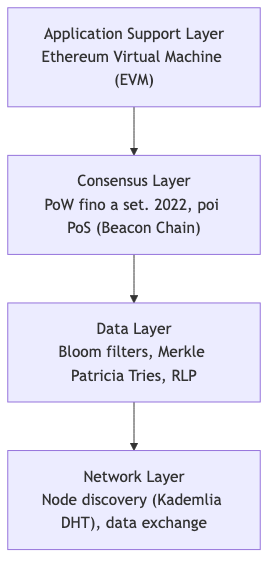
\includegraphics[keepaspectratio,alt={Diagramma Mermaid}]{images/mermaid-lezione-26-ethereum-2-0-fees-and-tries-01.png}}
\emph{Fig. --- I quattro livelli dell'architettura Ethereum.}

Il \textbf{Data Layer} è il focus della seconda parte della lezione:
comprende le strutture dati che rappresentano lo stato del sistema ---
account, transazioni, ricevute, storage dei contratti --- attraverso
strutture ad albero basate su Merkle Patricia Trie.

\begin{center}\rule{0.5\linewidth}{0.5pt}\end{center}

\section{Il Merkle Patricia Trie
(MPT)}\label{il-merkle-patricia-trie-mpt}

Il \textbf{Merkle Patricia Trie} è una struttura dati originale
introdotta nel Yellow Paper di Ethereum, che combina due strutture
classiche:

\begin{calloutdefinition}{Merkle Patricia Trie}

Albero che unisce il \textbf{Patricia Trie} (raggruppamento di prefissi
comuni delle chiavi per ricerca efficiente) con il \textbf{Merkle Tree}
(ogni nodo è l'hash dei propri figli, garantendo integrità e verifica
tamper-proof). È la struttura alla base di tutti i trie di Ethereum e
della maggior parte delle blockchain EVM-compatibili.

\end{calloutdefinition}

Il Patricia Trie evita di memorizzare ripetutamente sotto-cammini
comuni: nodi interni rappresentano prefissi condivisi, riducendo la
profondità dell'albero e velocizzando la ricerca. La struttura Merkle
garantisce che qualsiasi modifica a un dato foglia si propaghi cambiando
gli hash lungo tutto il cammino fino alla radice, rendendo ogni
manomissione immediatamente rilevabile.

\begin{center}\rule{0.5\linewidth}{0.5pt}\end{center}

\section{I due livelli di Ethereum
2.0}\label{i-due-livelli-di-ethereum-2.0}

Dopo il Merge, Ethereum è strutturato in due livelli distinti che
collaborano:

\subsection{Consensus Layer (Beacon
Chain)}\label{consensus-layer-beacon-chain}

Il Consensus Layer gestisce il protocollo di consenso PoS e la
validazione. Il suo blocco --- il \textbf{Beacon Block} --- non contiene
direttamente transazioni o ricevute, ma include un riferimento al blocco
dell'Execution Layer attraverso il campo
\texttt{execution\_payload\_header}.

\pandocbounded{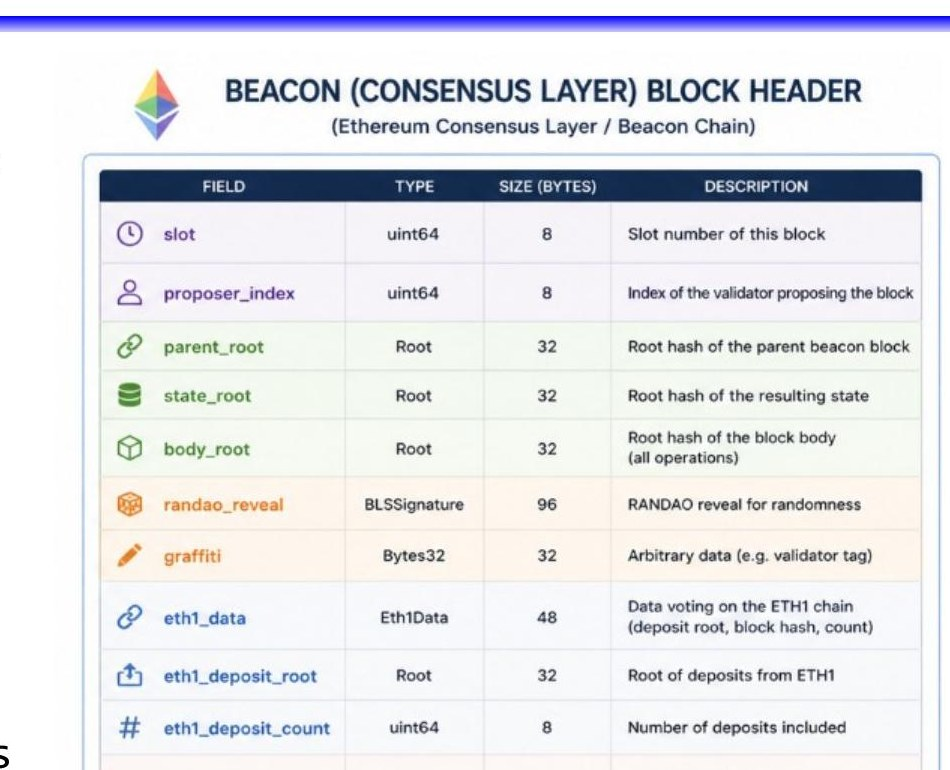
\includegraphics[keepaspectratio,alt={Beacon Block Header --- campi e tipi}]{images/lezione-26-ethereum-2-0-fees-and-tries-img-01.jpg}}
\emph{Fig. --- Struttura del Beacon Block Header: gestisce slot,
proposer, state root e il collegamento all'Execution Layer.}

\subsection{Execution Layer}\label{execution-layer}

L'Execution Layer gestisce le transazioni, i contratti intelligenti e i
log. Il suo block header è ricco di radici Merkle che certificano lo
stato del sistema:

\pandocbounded{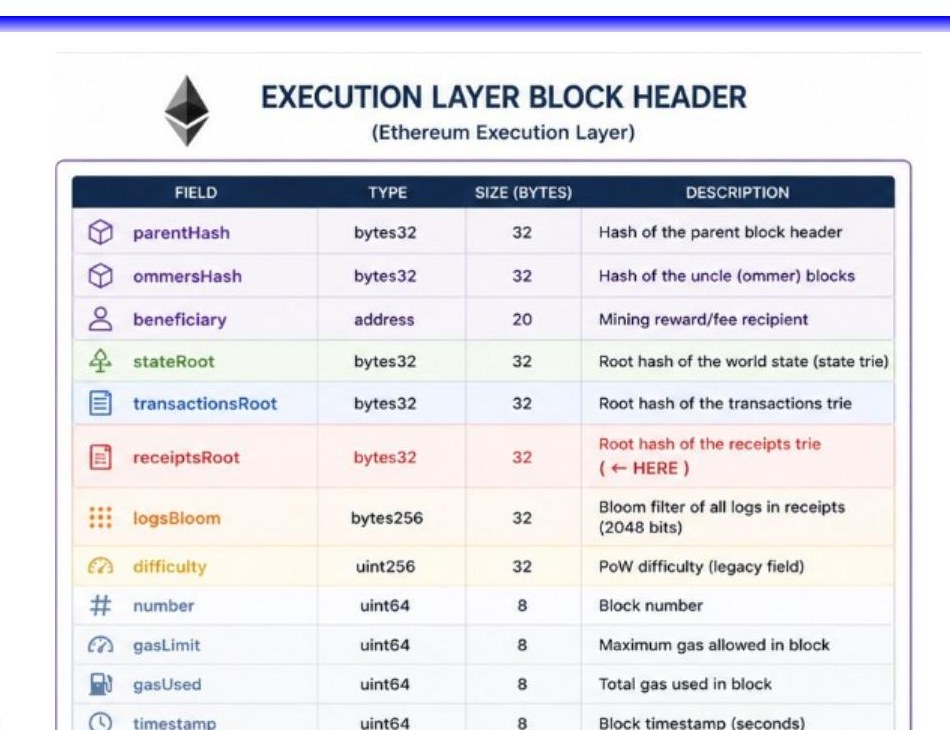
\includegraphics[keepaspectratio,alt={Execution Layer Block Header --- campi e tipi}]{images/lezione-26-ethereum-2-0-fees-and-tries-img-02.jpg}}
\emph{Fig. --- Struttura dell'Execution Layer Block Header: stateRoot,
transactionsRoot, receiptsRoot e logsBloom sono le radici dei trie
principali.}

I campi chiave per il Data Layer sono: - \texttt{stateRoot} → radice del
World State Trie - \texttt{transactionsRoot} → radice del Transaction
Trie - \texttt{receiptsRoot} → radice del Receipts Trie -
\texttt{logsBloom} → Bloom filter aggregato di tutti i log del blocco

\begin{center}\rule{0.5\linewidth}{0.5pt}\end{center}

\section{I Trie dell'Execution Layer}\label{i-trie-dellexecution-layer}

La slide seguente mostra la relazione tra il blocco e i quattro trie
principali:

\pandocbounded{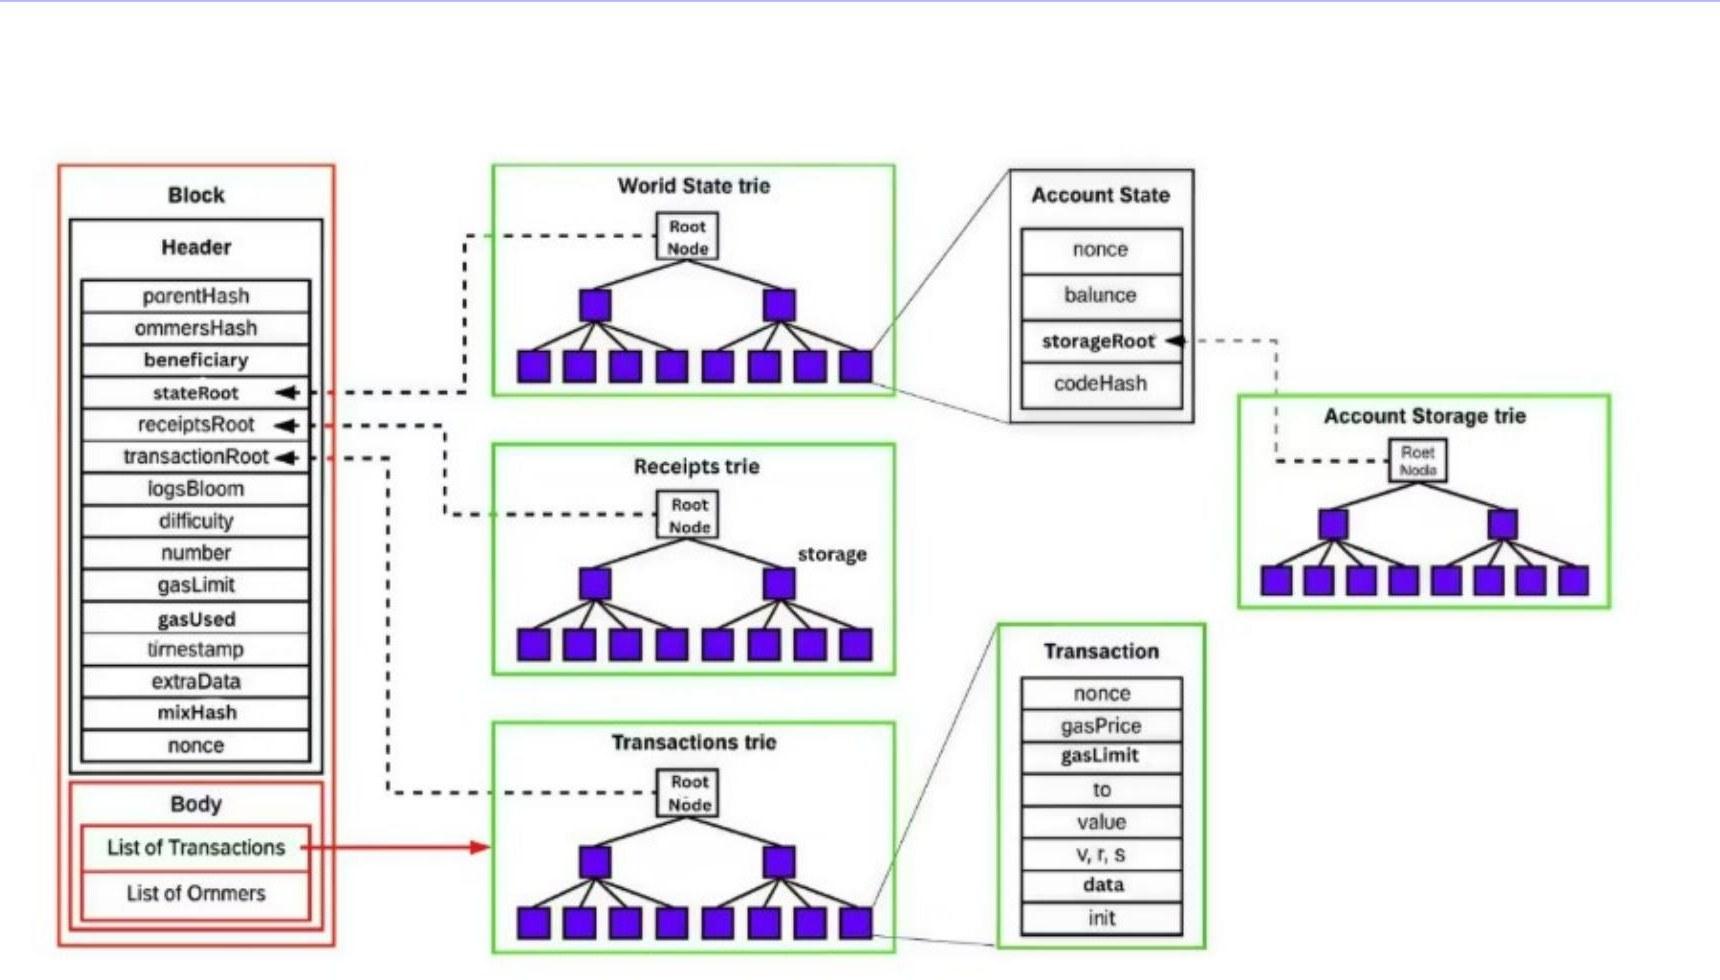
\includegraphics[keepaspectratio,alt={Diagramma dei trie dell'Execution Layer}]{images/lezione-26-ethereum-2-0-fees-and-tries-img-03.jpg}}
\emph{Fig. --- Il blocco punta tramite radici hash al World State Trie,
al Receipts Trie e al Transactions Trie. Il World State Trie punta
all'Account Storage Trie per ogni contratto.}

\pandocbounded{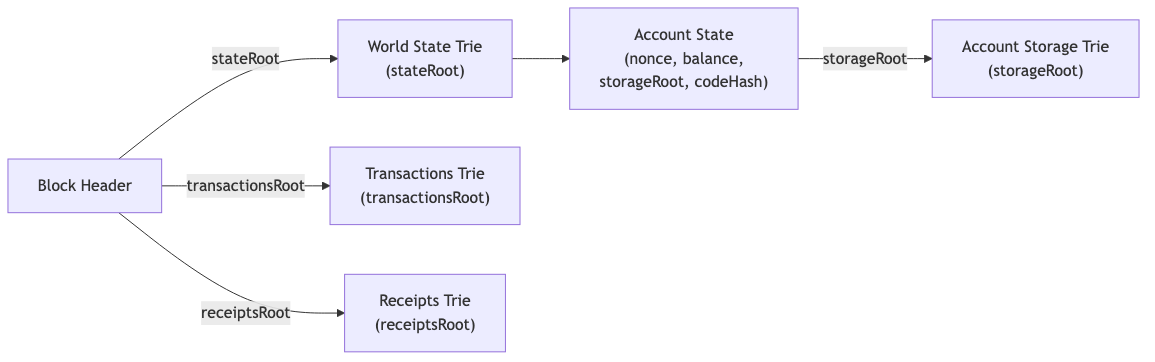
\includegraphics[keepaspectratio,alt={Diagramma Mermaid}]{images/mermaid-lezione-26-ethereum-2-0-fees-and-tries-02.png}}
\emph{Fig. --- Relazione tra Block Header e i quattro trie
dell'Execution Layer.}

\begin{calloutnote}{Quattro trie distinti}

\begin{itemize}
\tightlist
\item
  \textbf{World State Trie}: mappa ogni indirizzo → stato dell'account
  (nonce, balance, codeHash, storageRoot)
\item
  \textbf{Transaction Trie}: albero di tutte le transazioni del blocco;
  la radice è nel block header
\item
  \textbf{Receipts Trie}: albero delle ricevute di esecuzione (una per
  transazione)
\item
  \textbf{Account Storage Trie}: uno per ogni contratto, contiene le
  variabili di storage del contratto
\end{itemize}

\end{calloutnote}

\begin{center}\rule{0.5\linewidth}{0.5pt}\end{center}

\section{Il Transaction Trie}\label{il-transaction-trie}

Il Transaction Trie è un MPT che indicizza tutte le transazioni di un
blocco. Ogni transazione viene hashata, e gli hash vengono combinati
fino a produrre un unico \textbf{root hash} incluso nel block header.
Questo permette di: - Rilevare qualsiasi modifica a una transazione (il
root hash cambia) - Dimostrare l'appartenenza di una transazione a un
blocco senza scaricare il blocco completo (\textbf{Merkle proof}) -
Effettuare ricerche efficienti

\begin{center}\rule{0.5\linewidth}{0.5pt}\end{center}

\section{Logging e Transaction
Receipt}\label{logging-e-transaction-receipt}

\subsection{Perché i log}\label{perchuxe9-i-log}

Consideriamo un contratto NFT. I dati di proprietà corrente dei token
sono salvati nell'\textbf{account storage} --- lo stato on-chain
accessibile dal contratto. Ma altri tipi di informazione non richiedono
di essere nello storage del contratto:

\begin{itemize}
\tightlist
\item
  La \textbf{storia delle proprietà} interessa analisti e investitori,
  ma il contratto non ne ha bisogno durante l'esecuzione.
\item
  Le \textbf{notifiche al frontend} sono necessarie per confermare
  all'utente che un mint è avvenuto --- ma le transazioni sono
  asincrone, quindi il contratto non può restituire un valore
  direttamente all'interfaccia.
\end{itemize}

La soluzione è che il contratto \textbf{emetta un evento}
(\texttt{emit}), che viene scritto nei \textbf{log} della ricevuta di
transazione. Il frontend può ascoltare questi log e reagire.

\begin{callouttip}{Log vs Storage}

Il log storage è \textbf{molto più economico} dell'account storage in
termini di gas. È la scelta corretta per dati che non devono essere
letti dal contratto stesso, ma solo da applicazioni esterne (DApp,
analytics, indexer come The Graph).

\end{callouttip}

\subsection{Struttura del Transaction
Receipt}\label{struttura-del-transaction-receipt}

\begin{calloutdefinition}{Transaction Receipt}

Struttura dati che registra l'esito dell'esecuzione di una transazione
una volta inclusa in un blocco. Contiene: - \textbf{status}: 0 (fallita)
o 1 (successo) - \textbf{cumulativeGasUsed}: gas consumato da tutte le
transazioni precedenti nel blocco, inclusa quella corrente -
\textbf{logs}: lista di log entries emesse dal contratto durante
l'esecuzione - \textbf{logsBloom}: Bloom filter da 2048 bit costruito
sulle log entries, per ricerca rapida

\end{calloutdefinition}

\pandocbounded{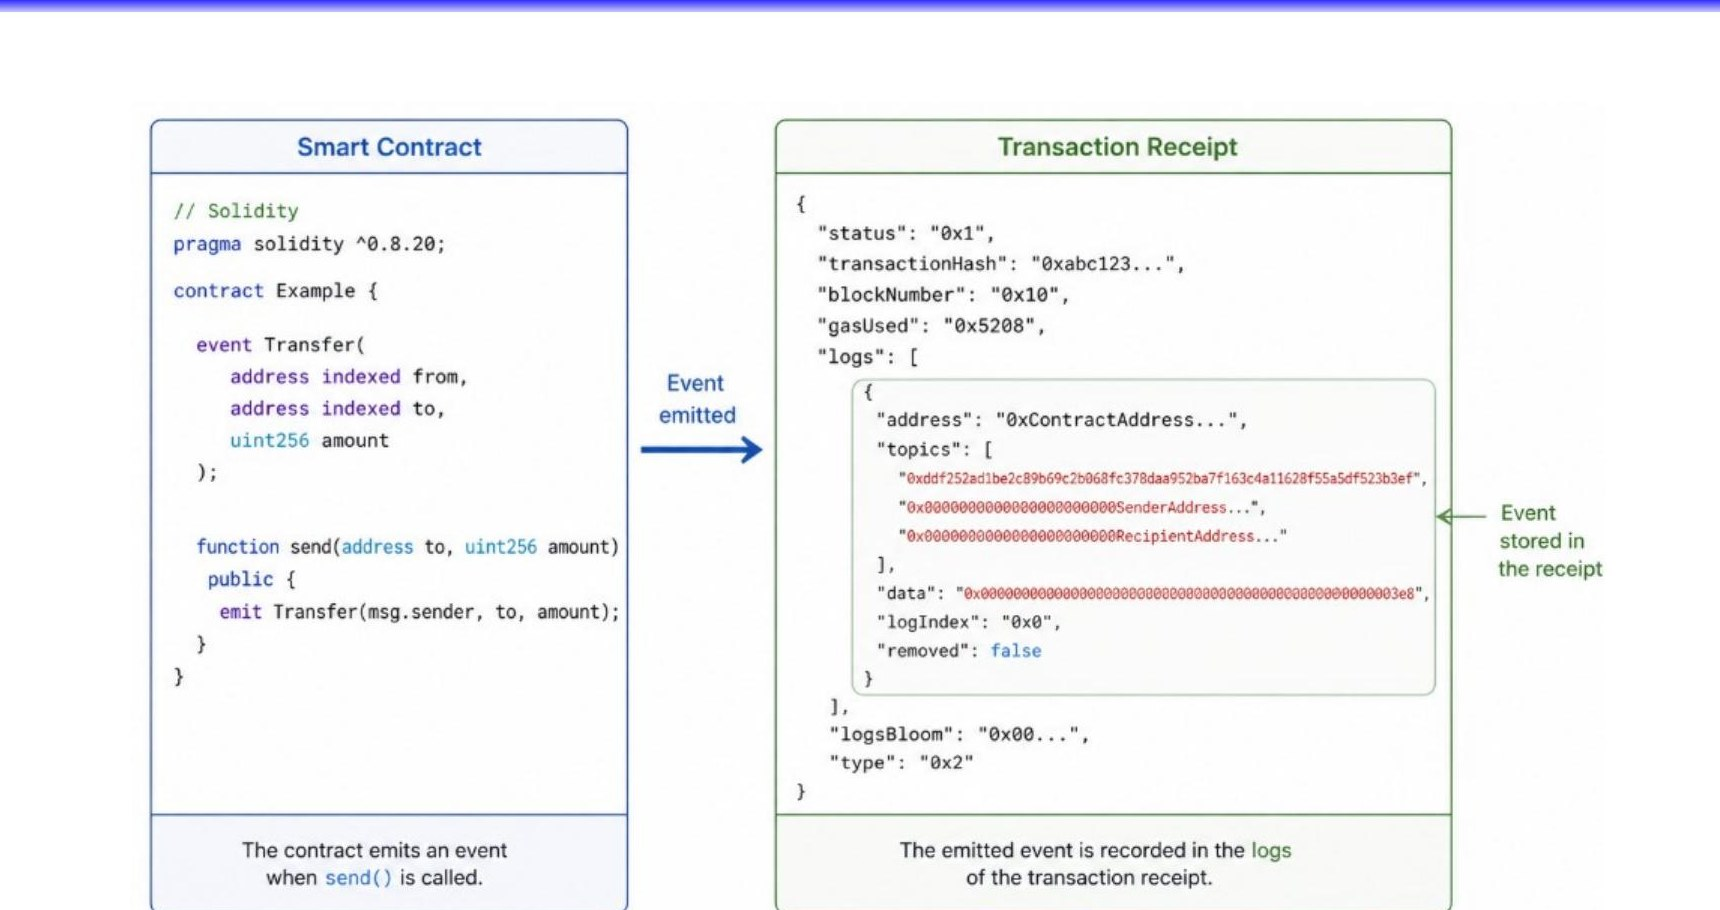
\includegraphics[keepaspectratio,alt={Smart Contract → Transaction Receipt}]{images/lezione-26-ethereum-2-0-fees-and-tries-img-04.jpg}}
\emph{Fig. --- Un contratto Solidity con evento Transfer emette il log
quando viene chiamata send(); il log viene registrato nella ricevuta
della transazione.}

\subsection{Status}\label{status}

Il campo \texttt{status} è 0 o 1. Poiché l'esecuzione è asincrona, il
chiamante deve attendere che il blocco venga incluso per leggere lo
status dalla ricevuta e determinare se la transazione ha avuto successo.

\subsection{cumulativeGasUsed}\label{cumulativegasused}

Il campo \texttt{gasUsed} nella ricevuta \textbf{non} è il gas consumato
dalla singola transazione: è il \textbf{totale cumulativo} di tutto il
gas utilizzato dalle transazioni dalla prima alla corrente nel blocco,
inclusa quest'ultima.

\pandocbounded{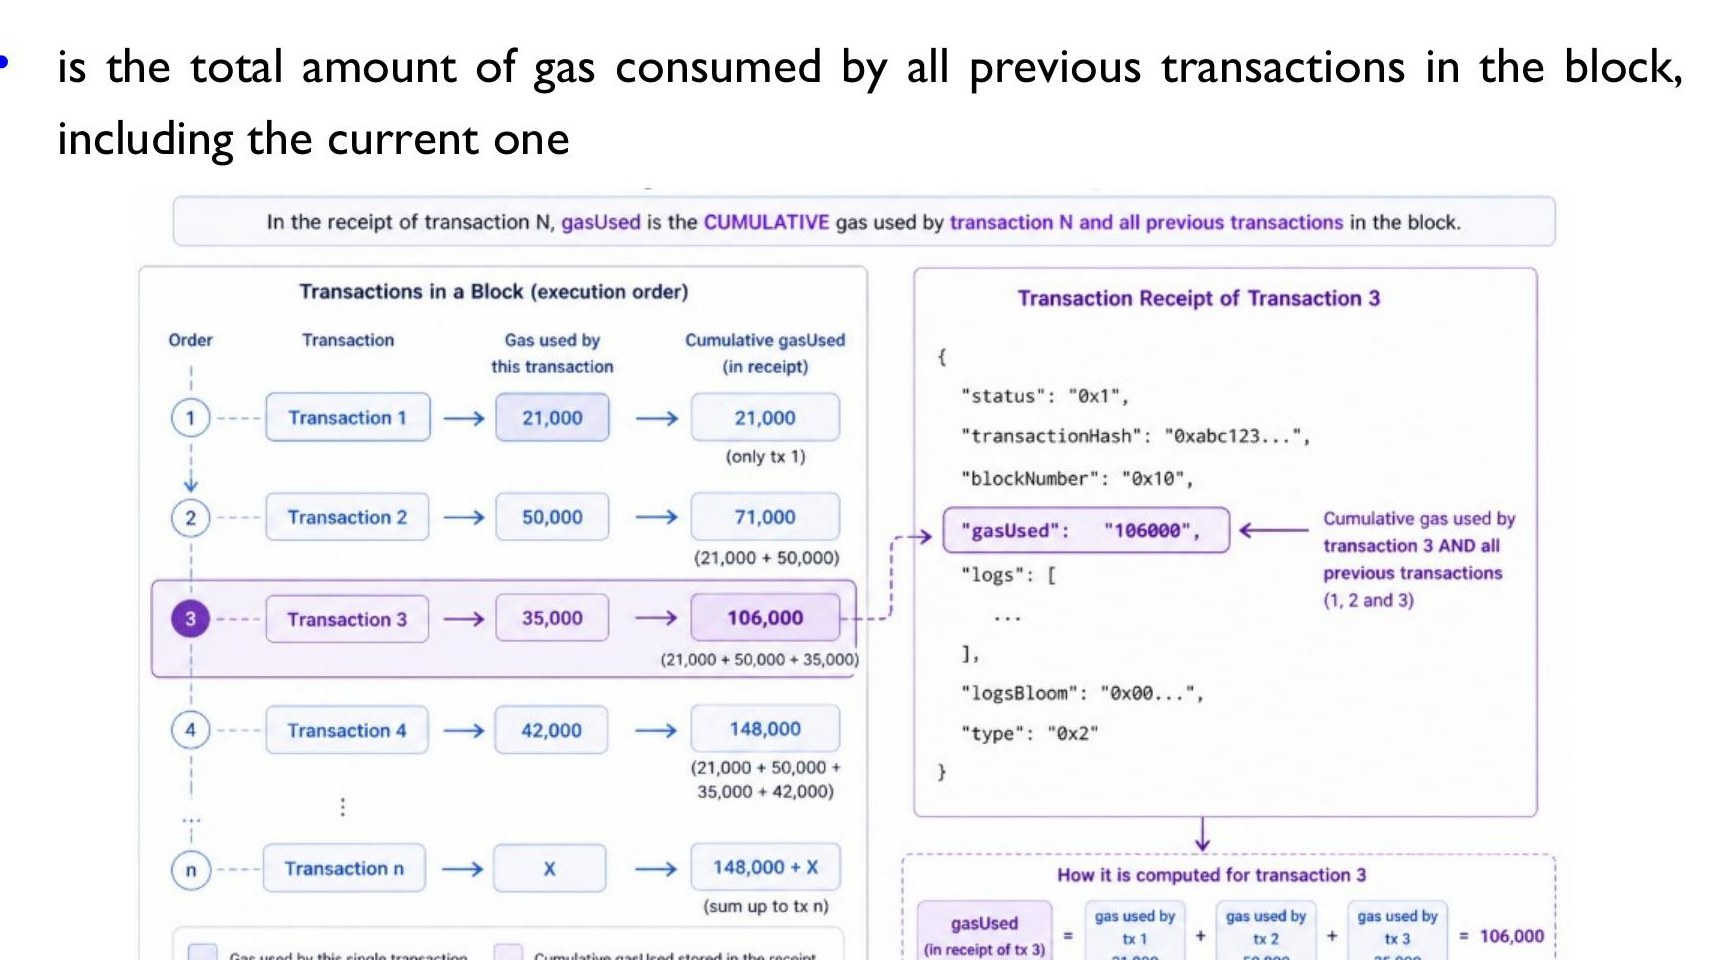
\includegraphics[keepaspectratio,alt={Schema gas cumulativo per transazione}]{images/lezione-26-ethereum-2-0-fees-and-tries-img-05.jpg}}
\emph{Fig. --- Per la transazione N, gasUsed nella ricevuta e la somma
del gas di tutte le transazioni da 1 a N. Nell'esempio, la ricevuta
della tx 3 riporta 106.000 gwei = 21.000 + 50.000 + 35.000.}

\begin{center}\rule{0.5\linewidth}{0.5pt}\end{center}

\section{I parametri Indexed e la struttura dei
Log}\label{i-parametri-indexed-e-la-struttura-dei-log}

\subsection{Parametri indexed in
Solidity}\label{parametri-indexed-in-solidity}

Nei contratti Solidity, i parametri di un evento possono essere
dichiarati \texttt{indexed}. Questo indica che quei valori devono essere
salvati nei \textbf{topics} del log (campi indicizzati), anziché nel
campo \texttt{data} generico.

\pandocbounded{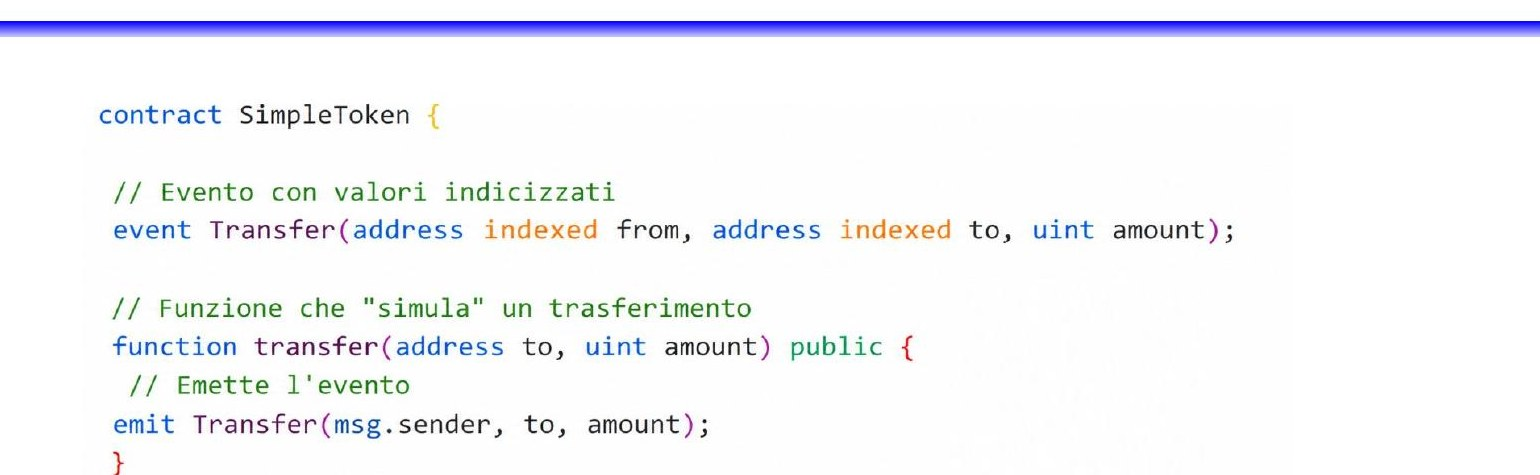
\includegraphics[keepaspectratio,alt={Codice Solidity con parametri indexed}]{images/lezione-26-ethereum-2-0-fees-and-tries-img-06.jpg}}
\emph{Fig. --- Nel contratto SimpleToken, from e to sono marcati indexed
--- vengono salvati nei topics della ricevuta per abilitare ricerche
efficienti.}

I parametri \texttt{indexed} abilitano \textbf{ricerche e filtraggio
efficienti}: per esempio, trovare tutti i trasferimenti di un token
effettuati da un dato indirizzo, oppure tutti i token venduti da un
utente. Sono salvati nei campi \texttt{topics} della ricevuta, mentre i
parametri non-indexed finiscono nel campo \texttt{data}.

\subsection{La struttura completa di un evento
loggato}\label{la-struttura-completa-di-un-evento-loggato}

\pandocbounded{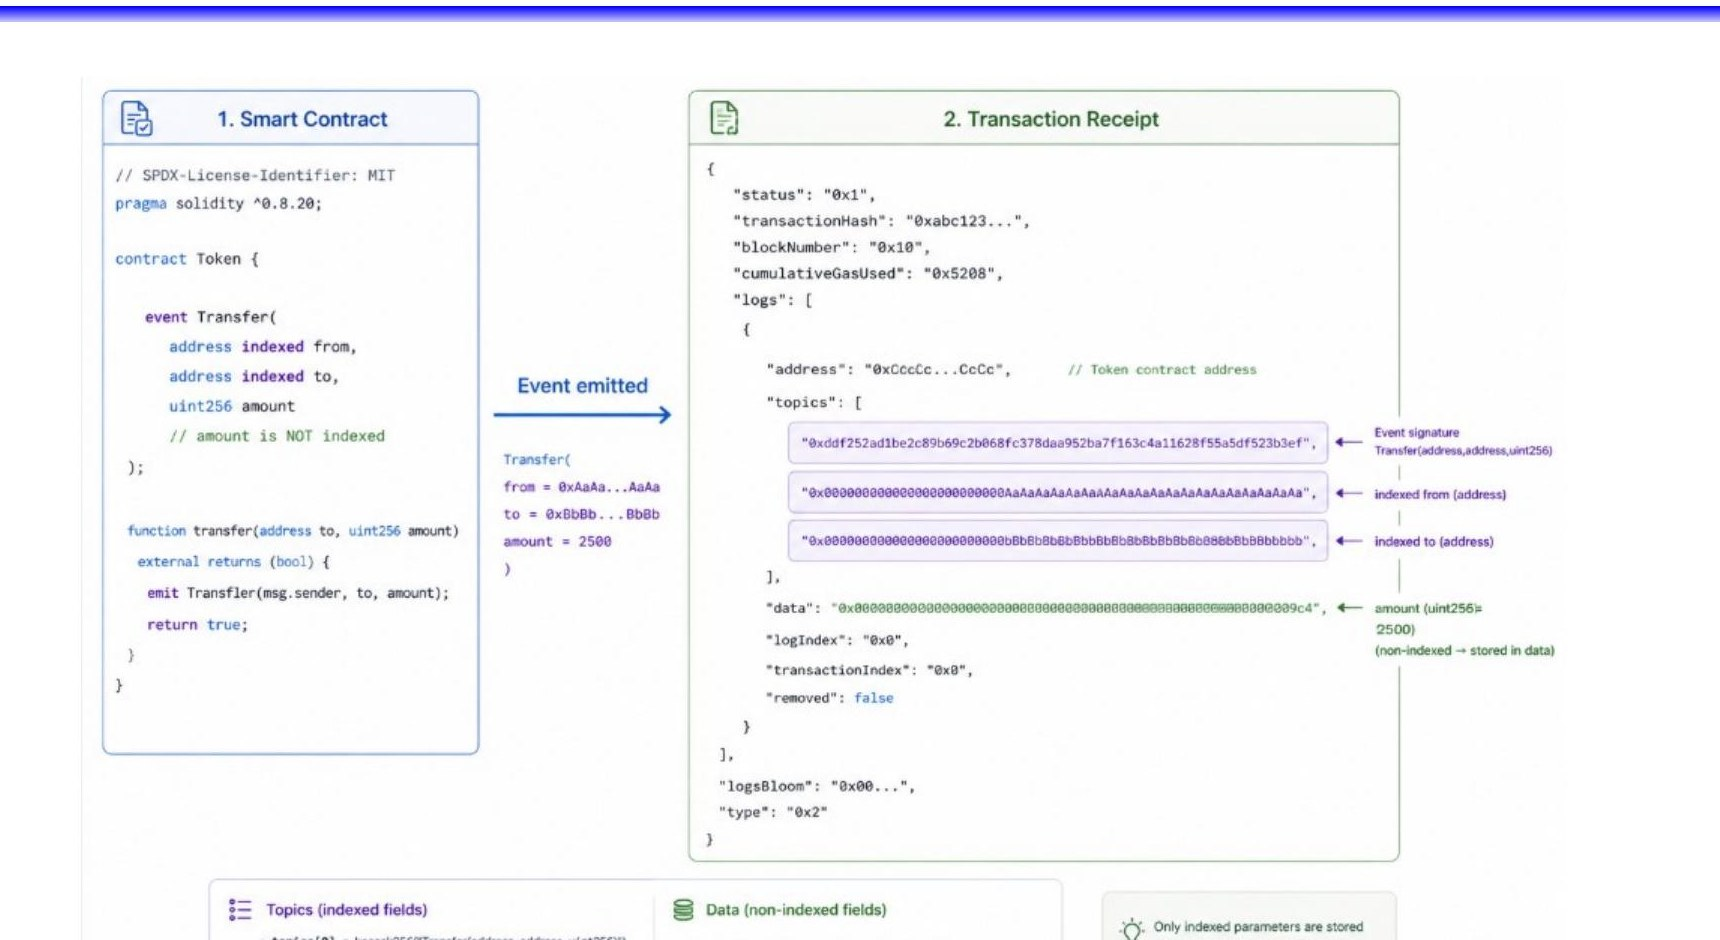
\includegraphics[keepaspectratio,alt={Evento Transfer --- struttura completa nella ricevuta}]{images/lezione-26-ethereum-2-0-fees-and-tries-img-07.jpg}}
\emph{Fig. --- A sinistra il contratto Token con l'evento Transfer; a
destra la ricevuta con topics (event signature + from + to) e data
(amount non-indexed).}

La struttura di un log entry nella ricevuta è: - \texttt{address}:
indirizzo del contratto che ha emesso l'evento - \texttt{topics{[}0{]}}:
keccak256 della firma dell'evento (es.
\texttt{Transfer(address,address,uint256)}) - \texttt{topics{[}1{]}},
\texttt{topics{[}2{]}}, \ldots: parametri \texttt{indexed} hashati -
\texttt{data}: parametri non-indexed codificati in ABI

\begin{center}\rule{0.5\linewidth}{0.5pt}\end{center}

\section{LogsBloom: filtraggio efficiente con Bloom
Filter}\label{logsbloom-filtraggio-efficiente-con-bloom-filter}

Cercare tutte le transazioni di un blocco che coinvolgono un certo
indirizzo richiederebbe di analizzare tutti i log di tutte le
transazioni --- un'operazione costosa. La soluzione è il
\textbf{logsBloom}: un {[}{[}Bloom Filter{]}{]} da 2048 bit (256 byte)
che riassume il contenuto dei log.

\subsection{LogsBloom nella ricevuta (livello
transazione)}\label{logsbloom-nella-ricevuta-livello-transazione}

\pandocbounded{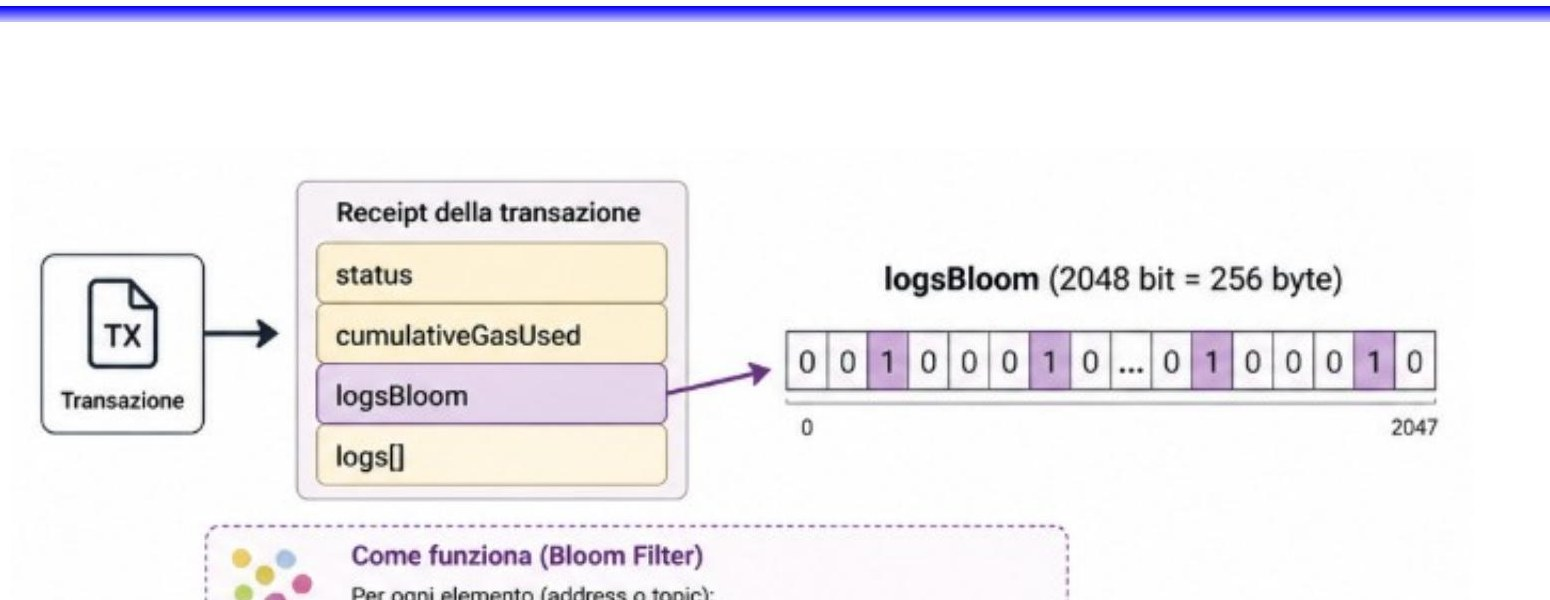
\includegraphics[keepaspectratio,alt={LogsBloom nella ricevuta --- Bloom Filter da 2048 bit}]{images/lezione-26-ethereum-2-0-fees-and-tries-img-08.jpg}}
\emph{Fig. --- Per ogni transazione, logsBloom e un Bloom filter
costruito sugli indirizzi e i topics dei log con keccak256 e 3 bit
impostati nel vettore da 2048 bit.}

Il processo di costruzione: 1. Per ogni elemento (address o topic) nei
log: calcola \texttt{keccak256(elemento)} 2. Deriva 3 posizioni nel
vettore da 2048 bit usando 3 hash diversi 3. Imposta a 1 i 3 bit
corrispondenti

\subsection{LogsBloom nel block header (livello
blocco)}\label{logsbloom-nel-block-header-livello-blocco}

\pandocbounded{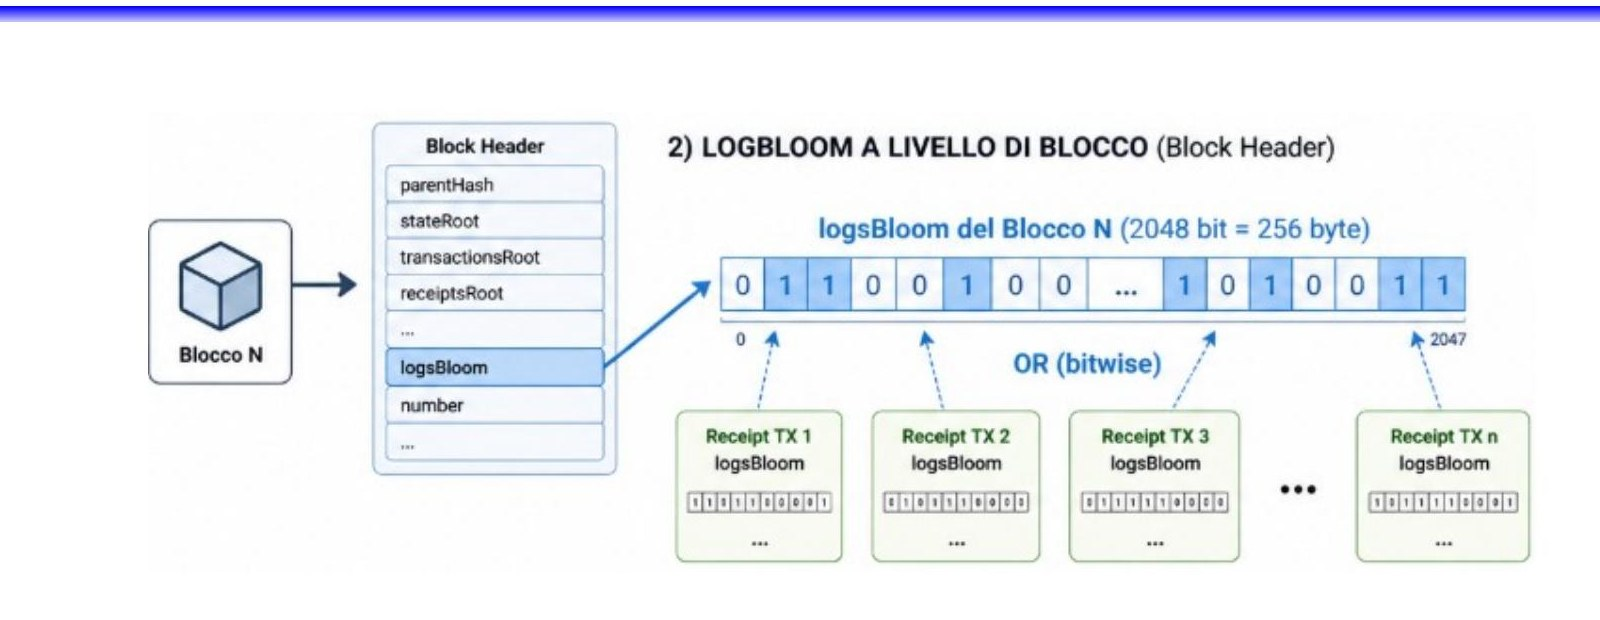
\includegraphics[keepaspectratio,alt={LogsBloom nel Block Header --- OR bitwise di tutti i receipt}]{images/lezione-26-ethereum-2-0-fees-and-tries-img-09.jpg}}
\emph{Fig. --- Il logsBloom del block header e l'OR bitwise dei
logsBloom di tutte le ricevute del blocco.}

Il \texttt{logsBloom} del block header è l'\textbf{OR bitwise} dei
logsBloom di tutte le ricevute nel blocco. Questo permette una ricerca a
due livelli: 1. Controlla il \texttt{logsBloom} del block header: se il
bit cercato è 0, il blocco non contiene quell'evento (nessun falso
negativo). 2. Solo se positivo, scendi a esaminare le singole ricevute.

\begin{calloutwarning}{Falsi positivi nel Bloom Filter}

Il Bloom Filter garantisce assenza di falsi negativi (se un elemento è
nel set, il filtro lo conferma sempre), ma ammette \textbf{falsi
positivi} (potrebbe indicare la presenza di un elemento che non c'è).
Per questo motivo, dopo aver trovato un blocco candidato tramite il
Bloom Filter, occorre verificare i dati effettivi.

\end{calloutwarning}

\begin{center}\rule{0.5\linewidth}{0.5pt}\end{center}

\section{Il Transaction Receipt Trie e il Storage
Trie}\label{il-transaction-receipt-trie-e-il-storage-trie}

\subsection{Il Transaction Receipt
Trie}\label{il-transaction-receipt-trie}

\pandocbounded{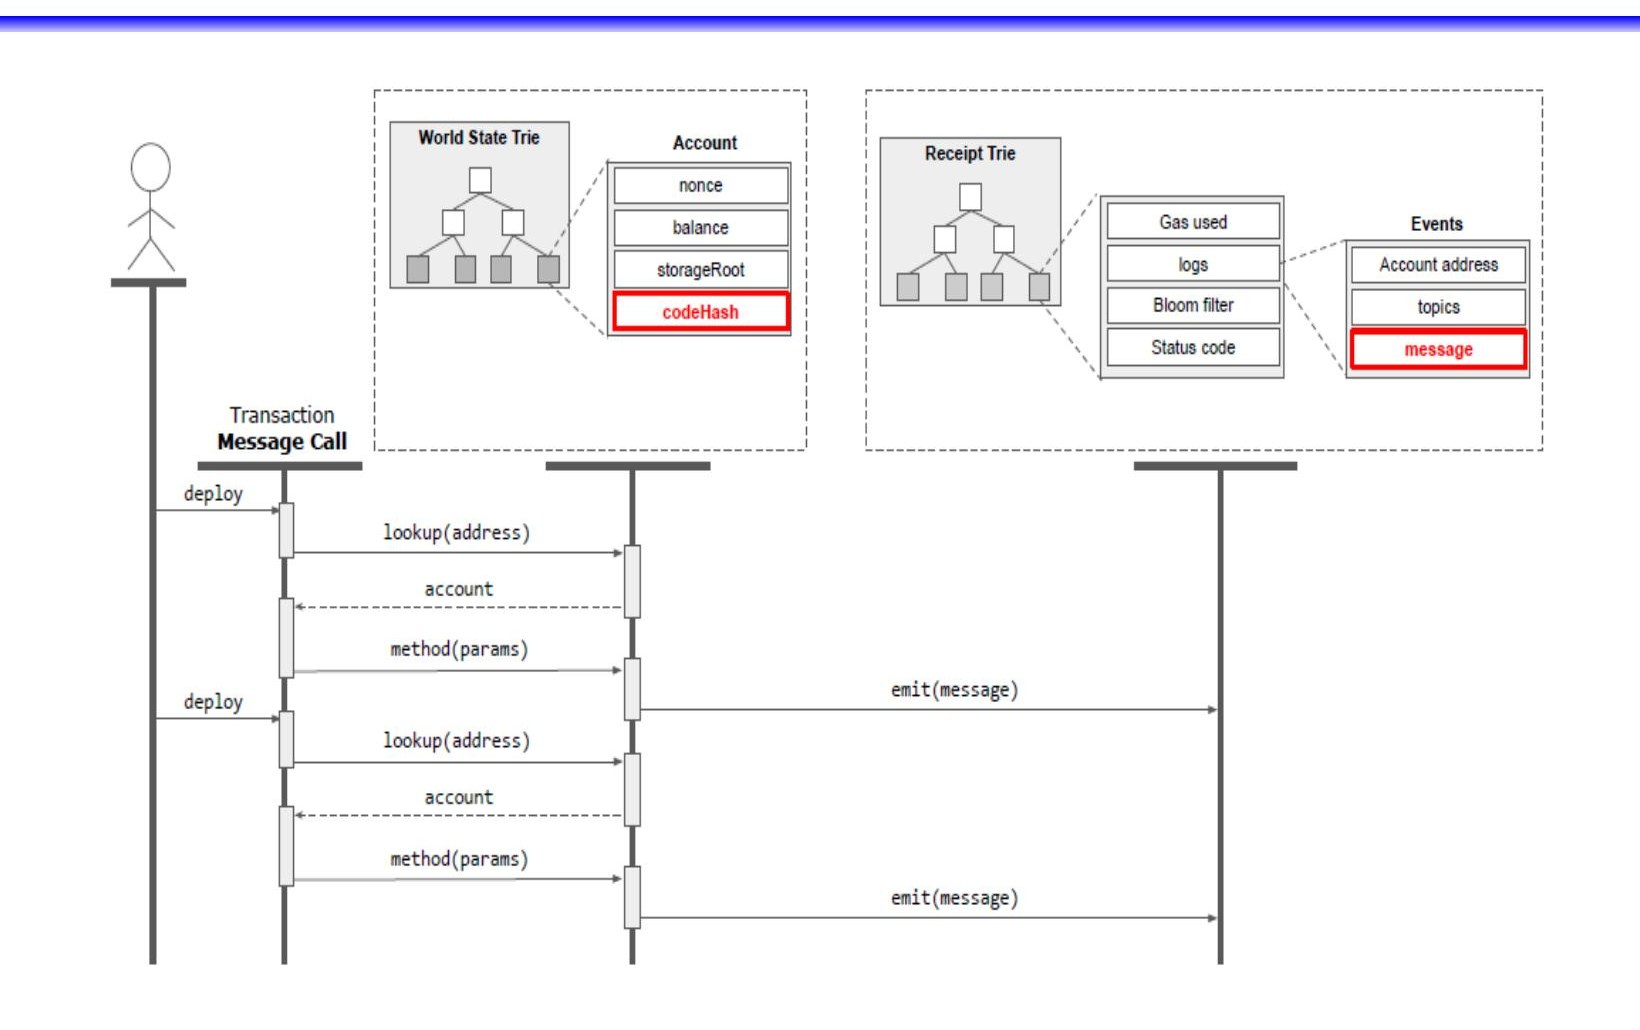
\includegraphics[keepaspectratio,alt={Transaction Receipt Trie --- sequence diagram}]{images/lezione-26-ethereum-2-0-fees-and-tries-img-10.jpg}}
\emph{Fig. --- Il Receipt Trie punta alle ricevute con Gas Used, Logs,
Bloom Filter e Status Code. Il sequence diagram mostra l'interazione
utente-World State Trie-Receipt Trie durante deploy multipli.}

Le ricevute di tutte le transazioni di un blocco sono indicizzate in un
MPT. La radice di questo trie è il campo \texttt{receiptsRoot} del block
header. Quando un utente vuole sapere se una transazione ha avuto
successo o vuole recuperare gli eventi emessi, può richiedere una Merkle
proof al nodo, senza dover scaricare l'intero blocco.

\subsection{Il Storage Trie}\label{il-storage-trie}

\pandocbounded{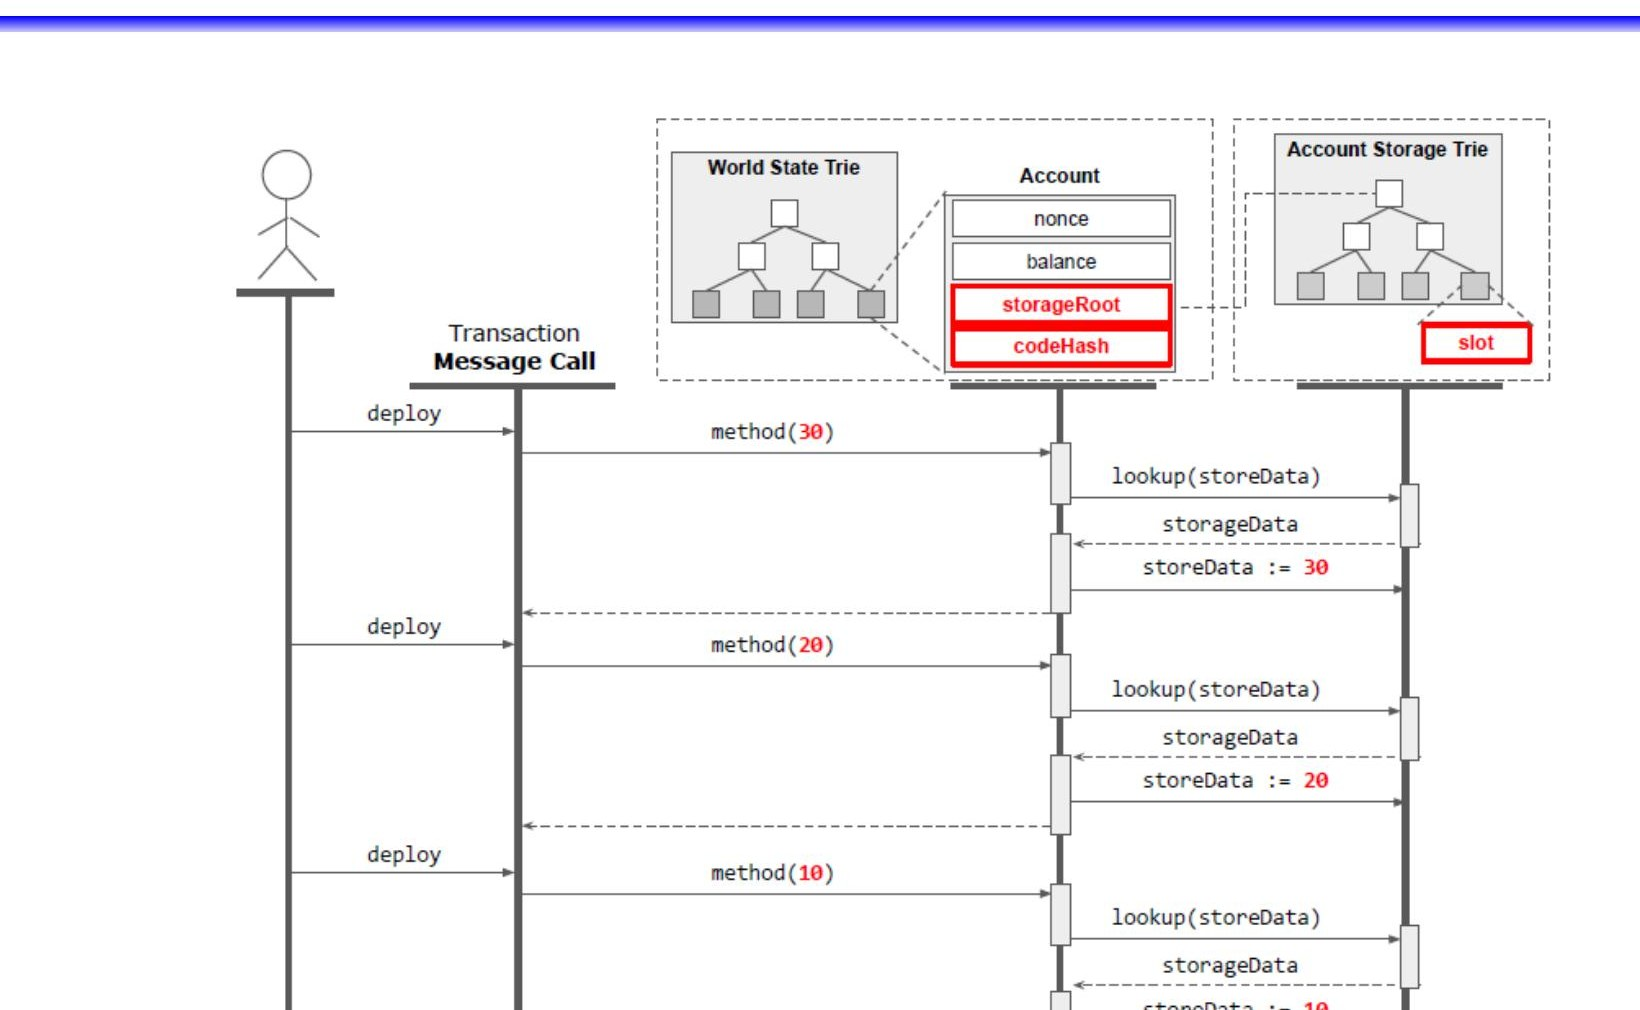
\includegraphics[keepaspectratio,alt={Storage Trie --- lettura/scrittura variabili contratto}]{images/lezione-26-ethereum-2-0-fees-and-tries-img-11.jpg}}
\emph{Fig. --- Il campo storageRoot punta all'Account Storage Trie con
uno slot per ogni contratto. Il sequence diagram mostra tre chiamate
successive con lookup e aggiornamento del valore.}

Ogni account contratto ha il proprio \textbf{Account Storage Trie}, a
cui si accede tramite il campo \texttt{storageRoot} dello World State
Trie. Ogni variabile di stato del contratto occupa uno \textbf{slot}
nell'albero. Ogni modifica di una variabile di storage aggiorna la
radice del trie dell'account, che a sua volta aggiorna la radice dello
World State Trie --- propagazione tipica della struttura Merkle.

\begin{center}\rule{0.5\linewidth}{0.5pt}\end{center}

\section{Bitcoin vs.~Ethereum: confronto
finale}\label{bitcoin-vs.-ethereum-confronto-finale}

\pandocbounded{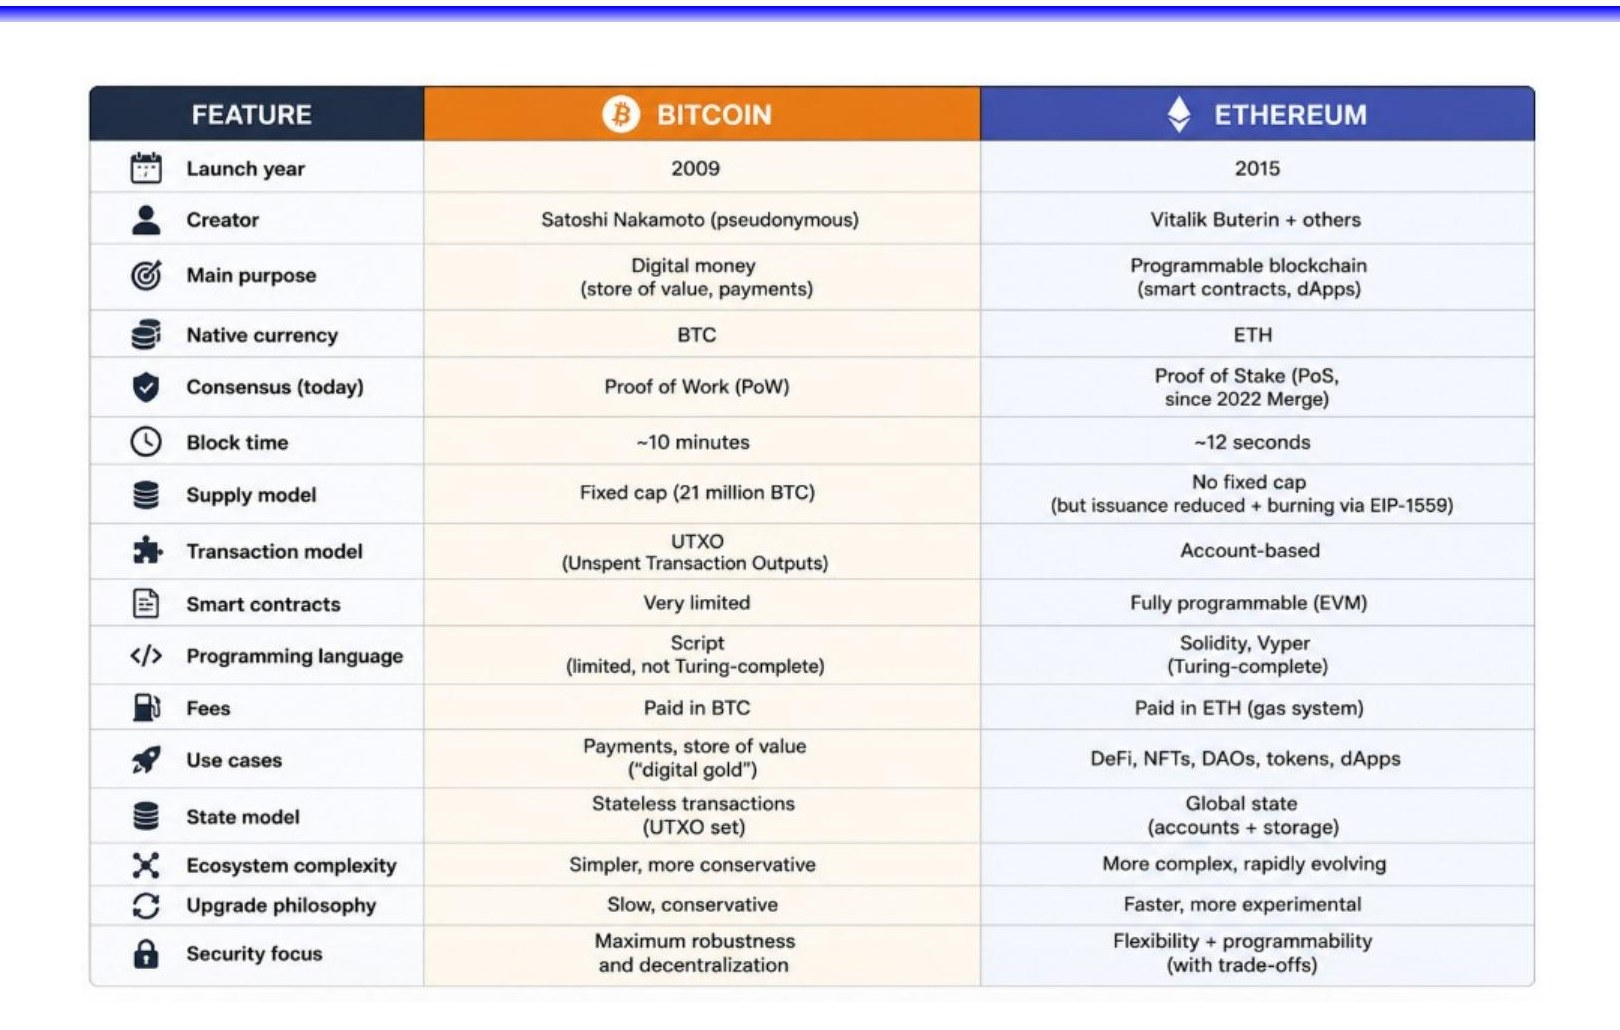
\includegraphics[keepaspectratio,alt={Tabella comparativa Bitcoin vs Ethereum}]{images/lezione-26-ethereum-2-0-fees-and-tries-img-12.jpg}}
\emph{Fig. --- Confronto su 14 dimensioni: anno di lancio, scopo,
consenso, block time, supply model, transaction model, smart contracts,
fees, use cases, state model e altro.}

\begin{calloutnote}{Differenze strutturali chiave}

\begin{itemize}
\tightlist
\item
  \textbf{Modello transazionale}: Bitcoin usa UTXO (Unspent Transaction
  Outputs), Ethereum usa un modello account-based con stato globale.
\item
  \textbf{Smart contract}: Bitcoin ha Script (limitato, non
  Turing-complete); Ethereum ha l'EVM con Solidity/Vyper
  (Turing-complete).
\item
  \textbf{Supply model}: Bitcoin ha un cap fisso di 21 milioni; Ethereum
  non ha cap fisso ma EIP-1559 introduce pressione deflazionistica
  tramite burn.
\item
  \textbf{Block time}: \textasciitilde10 minuti per Bitcoin,
  \textasciitilde12 secondi per Ethereum.
\item
  \textbf{Use cases}: Bitcoin è ottimizzato per pagamenti e riserva di
  valore (``digital gold''); Ethereum è una piattaforma programmabile
  per DeFi, NFT, DAO, dApp.
\end{itemize}

\end{calloutnote}

\newpage

\chapter{Applicazioni Reali con Smart
Contracts}\label{applicazioni-reali-con-smart-contracts}

Le criptovalute come Bitcoin, Ethereum e Solana rappresentano le
applicazioni più note della blockchain, ma si tratta soltanto del punto
di partenza. L'introduzione degli \textbf{smart contract} ha reso
possibile il passaggio da semplici transazioni finanziarie a sistemi
digitali completamente programmabili on-chain: supply chain, token
fungibili e non fungibili, finanza decentralizzata (DeFi),
organizzazioni governate da comunità (DAO) e identità digitale
auto-sovrana (SSI). La chiave di questa espansione è la
\textbf{composabilità}: diversi protocolli possono essere combinati tra
loro come moduli software, creando ecosistemi di applicazioni
interoperabili.

\begin{center}\rule{0.5\linewidth}{0.5pt}\end{center}

\section{Caso d'uso: Supply Chain}\label{caso-duso-supply-chain}

\subsection{Limiti dell'architettura
classica}\label{limiti-dellarchitettura-classica}

Il problema di partenza è concreto: un'azienda come Alpha Corporation
progetta e fa produrre macchinari complessi, li spedisce in sedi remote,
li sottopone a manutenzione periodica tramite terze parti autorizzate,
ne trasferisce la proprietà tra aziende diverse, e infine li dismette.
In un'architettura centralizzata classica, la sede centrale A1 gestisce
un database che traccia componenti, attrezzature, posizioni, storici di
manutenzione e ciclo di vita. Questo approccio presenta fragilità
strutturali: un attacco di tipo denial of service o una compromissione
del database può cancellare o alterare i record; i processi manuali
dipendono dalla memoria e dall'intervento umano; la conformità normativa
e l'auditing da parte di terzi sono difficili da garantire; le dispute
legali successive risultano costose e complesse perché l'auditabilità
del sistema non è garantita by design.

\subsection{Blockchain permissioned per la supply
chain}\label{blockchain-permissioned-per-la-supply-chain}

La soluzione proposta è una \textbf{blockchain permissioned}: una rete
P2P privata in cui solo i partecipanti autorizzati possono unirsi e
aggiungere blocchi. A differenza di una blockchain pubblica come
Ethereum, l'accesso è controllato da un'entità centralizzata --- in
questo caso Alpha --- che gestisce le chiavi pubbliche dei partecipanti
tramite un \textbf{Membership Service Provider (MSP)}.

\pandocbounded{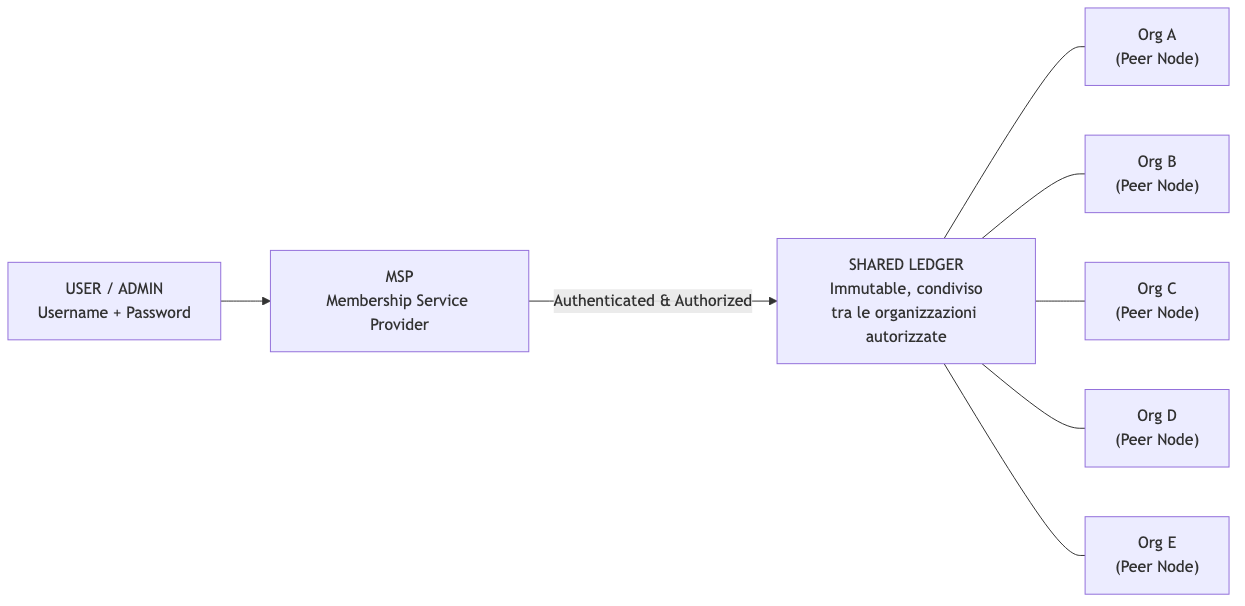
\includegraphics[keepaspectratio,alt={Diagramma Mermaid}]{images/mermaid-lezione-27-applicazioni-reali-con-smart-contracts-01.png}}
\emph{Fig. --- Architettura di una blockchain permissioned: ogni
organizzazione gestisce un peer node e condivide un ledger immutabile;
l'accesso è mediato dal Membership Service Provider (MSP).}

Il processo di bootstrap avviene in questo modo:

\begin{enumerate}
\def\labelenumi{\arabic{enumi}.}
\tightlist
\item
  \textbf{Alpha (A1)} avvia la blockchain creando il blocco genesi, che
  contiene la propria chiave pubblica. Questa chiave servirà ad
  autenticare tutti i dati registrati da A1 in futuro.
\item
  \textbf{A2} (la fabbrica) e \textbf{B} (l'azienda di manutenzione)
  generano coppie di chiavi pubblica/privata e inviano le chiavi
  pubbliche ad A1, che le annuncia sulla blockchain. Da questo momento
  A2 e B sono nodi della rete P2P, gestiscono il proprio nodo blockchain
  e possono aggiungere blocchi.
\item
  Nessun partecipante conosce le chiavi private degli altri:
  l'impersonificazione è impossibile per costruzione crittografica.
\end{enumerate}

\subsubsection{Identificazione dei componenti e
IoT}\label{identificazione-dei-componenti-e-iot}

Ogni componente prodotto da A2 riceve una propria coppia di chiavi: la
chiave pubblica viene annunciata sulla blockchain insieme alla posizione
iniziale (magazzino della fabbrica), mentre la chiave privata può essere
fisicamente incorporata nel componente. A seconda del valore del
componente, la comunicazione con la blockchain avviene in modo diverso:

\begin{itemize}
\tightlist
\item
  \textbf{Componenti economici}: codice QR con la chiave pubblica;
  lettori RFID leggono la chiave e inviano report alla blockchain per
  conto del componente.
\item
  \textbf{Componenti costosi}: tag RFID attivo con connettività
  Bluetooth; il componente può autonomamente contattare dispositivi
  vicini e inviare report on-chain.
\item
  \textbf{Macchinario completo}: dispositivo IoT completamente connesso
  con GPS integrato, eventualmente un nodo blockchain leggero, e un
  lettore RFID integrato che scansiona tutti i componenti interni e
  rileva eventuali sostituzioni.
\end{itemize}

\subsubsection{Smart contract e automazione della
manutenzione}\label{smart-contract-e-automazione-della-manutenzione}

Quando un componente viene registrato sulla blockchain, all'annuncio
della sua chiave pubblica può essere allegato uno smart contract. Questo
contratto può innescare automaticamente richieste di manutenzione,
ordini di sostituzione o procedure di dismissione senza intervento
umano.

\pandocbounded{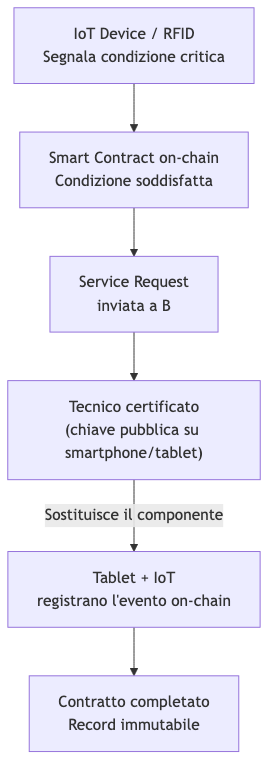
\includegraphics[keepaspectratio,alt={Diagramma Mermaid}]{images/mermaid-lezione-27-applicazioni-reali-con-smart-contracts-02.png}}
\emph{Fig. --- Flusso di automazione: dal rilevamento della condizione
critica (IoT) all'esecuzione dello smart contract, fino alla
registrazione immutabile dell'intervento.}

\subsubsection{Revoca delle
certificazioni}\label{revoca-delle-certificazioni}

Se un tecnico lascia l'azienda B, il responsabile pubblica un messaggio
di revoca della chiave sul blocco, firmato con la propria chiave
privata. Tutti i record precedenti al blocco di revoca rimangono validi
e immutabili; i record successivi firmati con la chiave revocata non
sono più considerati autentici.

\subsubsection{Trasferimento di proprietà e
decommissioning}\label{trasferimento-di-proprietuxe0-e-decommissioning}

Quando il macchinario cambia proprietario (dall'azienda X alla Y),
l'evento viene registrato sulla blockchain, creando un registro
immutabile di provenienza. Al termine del ciclo di vita, la dismissione
viene certificata con la firma del produttore originale A, consentendo
futuri audit ambientali e di conformità normativa. Al termine
dell'intero processo esiste sulla blockchain un registro completo di
tutti i partecipanti, componenti, posizioni, interventi e trasferimenti:
i record non possono essere alterati né cancellati, e non esiste un
single point of failure.

\begin{center}\rule{0.5\linewidth}{0.5pt}\end{center}

\section{Certificazione e
Tracciabilità}\label{certificazione-e-tracciabilituxe0}

Oltre alla supply chain industriale, la blockchain trova applicazione
ovunque sia necessaria la \textbf{tracciabilità} di prodotti lungo
l'intera catena di distribuzione e la \textbf{prova di autenticità} a
prova di manomissione. I settori principali includono: alimentare e
agricoltura, farmaceutica, manifattura industriale, edilizia e BIM (dove
si tracciano materiali, certificazioni e dati del ciclo di vita
dell'edificio), beni di lusso e diamanti.

\begin{calloutnote}{EU Digital Product Passport}

L'Unione Europea sta valutando il Digital Product Passport (DPP) per
tracciare sostenibilità e provenienza dei prodotti. I pilot attuali
esplorano blockchain, Decentralized Identifiers (DID), Verifiable
Credentials e smart contract. Lo scenario più realistico prevede
architetture ibride: database centralizzati con prove su blockchain,
reti DLT permissioned e standard di interoperabilità come EBSI.

\end{calloutnote}

\begin{center}\rule{0.5\linewidth}{0.5pt}\end{center}

\section{NFT: Arte Digitale e
Proprietà}\label{nft-arte-digitale-e-proprietuxe0}

Un'opera d'arte digitale è banalmente copiabile: chiunque può farne
screenshot o download. Ma \textbf{copiare non significa possedere}. In
un sistema tradizionale, la proprietà resta all'artista o a chi detiene
il copyright, indipendentemente da quante copie circolino. L'analogia
fisica è la prima edizione di un libro: ha lo stesso contenuto di tutte
le ristampe, ma vale di più.

Gli \textbf{NFT} (Non Fungible Token, token non fungibili) estendono
questo concetto al digitale. Quando Beeple ha mintato il suo NFT per
l'opera \emph{Everydays: The First 5000 Days}, ha creato un token sulla
blockchain contenente: - Un \textbf{fingerprint unico} del file
dell'opera (\texttt{8a5de7b183ecf2ec9f488}) - Il nome del token:
\texttt{Everydays:\ The\ First\ 5000\ Days} - Il simbolo:
\texttt{EF5000D}

La transazione sulla blockchain registra che ``il token
\texttt{8a5de7b183ecf2ec9f488} è creato da Beeple, che ne è il
proprietario.'' L'opera stessa \textbf{non è nel blocco}: l'NFT contiene
solo un link al file archiviato su un file system distribuito (IPFS o
equivalente). Ciò che si acquista è il certificato di proprietà, non il
file --- esattamente come comprare la chitarra di Elvis Presley:
chiunque può comprare una chitarra identica, ma solo una ha quel
certificato di autenticità.

\begin{center}\rule{0.5\linewidth}{0.5pt}\end{center}

\section{DeFi --- Finanza
Decentralizzata}\label{defi-finanza-decentralizzata}

La \textbf{DeFi} (Decentralized Finance) è l'insieme di applicazioni
finanziarie costruite su blockchain che eliminano intermediari
tradizionali come banche, broker e exchange, sostituendoli con smart
contract e protocolli automatizzati.

\subsection{Stable Coin}\label{stable-coin}

Le criptovalute tradizionali sono altamente volatili. Una \textbf{stable
coin} è progettata per mantenere un valore stabile, tipicamente
agganciato a una valuta fiat (1 coin = 1 USD). Questo permette di
integrare valute reali nelle applicazioni on-chain e offre a persone in
paesi con alta inflazione un'alternativa digitale al dollaro senza
necessitare di un conto bancario statunitense.

\begin{calloutdefinition}{Tipi di Stable Coin}

{\def\LTcaptype{none} % do not increment counter
\begin{longtable}[]{@{}
  >{\raggedright\arraybackslash}p{(\linewidth - 6\tabcolsep) * \real{0.1818}}
  >{\raggedright\arraybackslash}p{(\linewidth - 6\tabcolsep) * \real{0.2727}}
  >{\raggedright\arraybackslash}p{(\linewidth - 6\tabcolsep) * \real{0.3030}}
  >{\raggedright\arraybackslash}p{(\linewidth - 6\tabcolsep) * \real{0.2424}}@{}}
\toprule\noalign{}
\begin{minipage}[b]{\linewidth}\raggedright
Tipo
\end{minipage} & \begin{minipage}[b]{\linewidth}\raggedright
Backing
\end{minipage} & \begin{minipage}[b]{\linewidth}\raggedright
Custodia
\end{minipage} & \begin{minipage}[b]{\linewidth}\raggedright
Esempi
\end{minipage} \\
\midrule\noalign{}
\endhead
\bottomrule\noalign{}
\endlastfoot
\textbf{Fiat-Collateralized} & Valute fiat 1:1 in riserva presso un ente
& Custodial & USDC, USDT, BUSD \\
\textbf{Commodity-Backed} & Materie prime fisiche (oro, argento) &
Custodial & PAXG, XAUT \\
\textbf{Crypto-Collateralized} & Crypto bloccate in smart contract
(over-collateralized) & Non-custodial & DAI, LUSD \\
\textbf{Algorithmic} & Algoritmi + incentivi di mercato & Non-custodial
& FRAX, AMPL \\
\end{longtable}
}

\end{calloutdefinition}

\subsubsection{Fiat-Backed: ciclo di vita
completo}\label{fiat-backed-ciclo-di-vita-completo}

Il ciclo di vita di una stable coin fiat-backed si articola in tre
operazioni governate da uno smart contract \textbf{ERC-20}:

\textbf{Minting} --- Bob deposita 100 USD e Alice 35 USD presso il
custodian (la banca). Il custodian chiama \texttt{mint(Bob,\ 100)} e
\texttt{mint(Alice,\ 35)} sul contratto ERC-20. Il contratto aggiorna il
mapping \texttt{\_balances} on-chain. La riserva del custodian ammonta a
135 USD.

\textbf{Transfer} --- Bob paga 15 USDC a Carol chiamando
\texttt{transfer(Bob\ →\ Carol,\ 15)} sul contratto (pagando la gas
fee). Il trasferimento avviene completamente on-chain senza coinvolgere
il custodian: i saldi diventano Bob: 85, Alice: 35, Carol: 15.

\textbf{Withdrawal} --- Bob ritira 60 USD reali. Il custodian chiama
\texttt{burn(Bob,\ 60)} sul contratto, distruggendo i token. Il saldo di
Bob scende a 25 USDC, la riserva del custodian si riduce a 75 USD, e Bob
riceve 60 USD fisici.

\pandocbounded{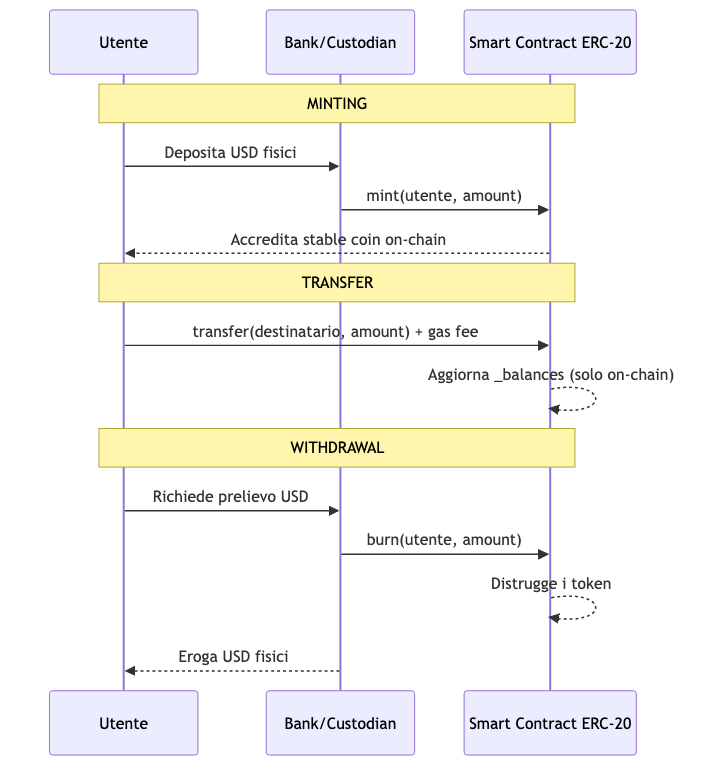
\includegraphics[keepaspectratio,alt={Diagramma Mermaid}]{images/mermaid-lezione-27-applicazioni-reali-con-smart-contracts-03.png}}
\emph{Fig. --- Ciclo completo di una stable coin fiat-backed: il minting
e il withdrawal coinvolgono il custodian; il trasferimento è puramente
on-chain.}

\subsubsection{Stabilità tramite
arbitraggio}\label{stabilituxe0-tramite-arbitraggio}

Le stable coin fiat-backed mantengono il peg attraverso
l'\textbf{arbitraggio}: se 1 USDC vale 1,02 USD sul mercato secondario,
i trader acquistano USD dalla banca a 1:1 e vendono USDC sul mercato,
spingendo il prezzo verso il basso. Il meccanismo inverso vale quando il
prezzo scende sotto il peg.

\subsubsection{Crypto-Collateralized}\label{crypto-collateralized}

Le stable coin crypto-collateralized sono decentralizzate e
non-custodial: il collaterale è bloccato in smart contract, non presso
una banca. Poiché le criptovalute sono volatili, è richiesta la
\textbf{over-collateralization}: per mintare 100 USD di stable coin
occorre depositare 150 USD di ETH. Se il valore del collaterale scende
sotto la soglia di sicurezza, la posizione viene liquidata
automaticamente.

\subsubsection{Algorithmic Stable Coin}\label{algorithmic-stable-coin}

Le stable coin algoritmiche mantengono il peg senza riserve complete,
usando algoritmi, smart contract e meccanismi di arbitraggio. Un oracolo
monitora il prezzo di mercato e lo invia on-chain: se il prezzo supera
il peg, l'offerta aumenta; se scende al di sotto, l'offerta si riduce.

\begin{center}\rule{0.5\linewidth}{0.5pt}\end{center}

\subsection{Lending e Borrowing}\label{lending-e-borrowing}

I protocolli DeFi di lending replicano on-chain la funzione delle banche
commerciali: chi ha liquidità la presta guadagnando interessi; chi ha
asset ma non vuole venderli ottiene liquidità depositando collaterale.
Il sistema coinvolge quattro attori: lender, borrower, price oracle e
liquidator.

\pandocbounded{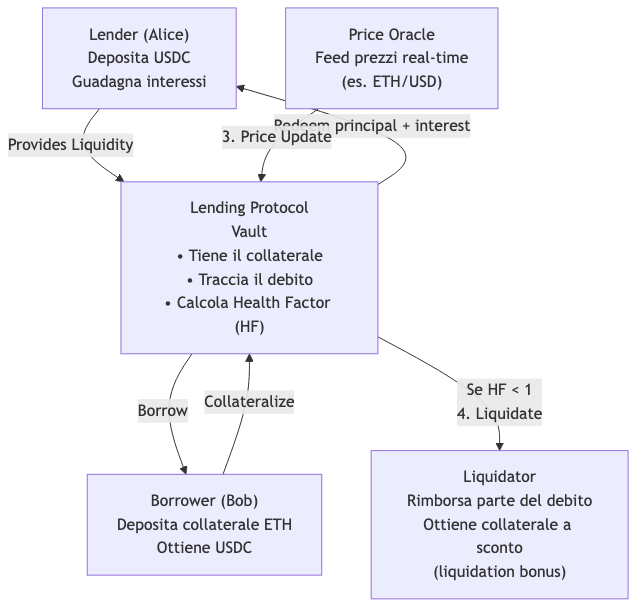
\includegraphics[keepaspectratio,alt={Diagramma Mermaid}]{images/mermaid-lezione-27-applicazioni-reali-con-smart-contracts-04.png}}
\emph{Fig. --- Modello generale del lending DeFi: il vault gestisce
collaterale e debito; l'oracle fornisce prezzi; il liquidator interviene
quando il Health Factor scende sotto 1.}

\subsubsection{Il lender}\label{il-lender}

Il lender deposita asset liquidi (es. 50.000 USDC) nel protocollo e
riceve in cambio token di interesse. Nel tempo accumula rendimento
proporzionale alla liquidità fornita e alla domanda di prestito.

\subsubsection{Il borrower e
l'over-collateralization}\label{il-borrower-e-lover-collateralization}

Il borrower deposita collaterale (es. 10 ETH a \$3.000 = \$30.000) e
ottiene liquidità (es. 20.000 USDC) senza vendere i propri asset. La
motivazione è strategica: Bob vede i suoi BTC o ETH come asset con
potenziale di apprezzamento a lungo termine e preferisce ottenerci
liquidità piuttosto che venderli. Il protocollo traccia il
\textbf{Health Factor (HF)}:

\[HF = \frac{   ext{Valore collaterale}     imes    ext{Liquidation threshold}}{    ext{Valore debito}}\]

Quando \(HF < 1\), la posizione è sottocollateralizzata e diventa
liquidabile.

\subsubsection{Il liquidatore}\label{il-liquidatore}

Se il mercato crolla e il collaterale scende sotto soglia (es. ETH da
\$3.000 a \$2.200, collaterale vale \$22.000 ma debito è ancora
\$20.000), il protocollo consente a qualsiasi liquidatore di
intervenire:

\begin{enumerate}
\def\labelenumi{\arabic{enumi}.}
\tightlist
\item
  Alice (liquidator) rimborsa 5.000 USDC del debito di Bob.
\item
  Il protocollo dà ad Alice ETH per \$5.500 (liquidation bonus del
  10\%).
\item
  Bob perde parte del collaterale, ma il suo debito si riduce; Alice
  guadagna il bonus; il protocollo rimane solvente.
\end{enumerate}

\begin{calloutwarning}{Il ruolo critico dell’oracle}

Per calcolare il Health Factor in tempo reale, il protocollo deve
conoscere il prezzo corrente dell'ETH. Ma una blockchain è un ``database
isolato'' senza connessione a Internet. La soluzione sono i
\textbf{blockchain oracle}: servizi che portano dati off-chain (prezzi
di mercato, risultati sportivi, orari voli) on-chain in modo sicuro.

\end{calloutwarning}

\subsubsection{Blockchain Oracle --- use
case}\label{blockchain-oracle-use-case}

{\def\LTcaptype{none} % do not increment counter
\begin{longtable}[]{@{}
  >{\raggedright\arraybackslash}p{(\linewidth - 2\tabcolsep) * \real{0.4000}}
  >{\raggedright\arraybackslash}p{(\linewidth - 2\tabcolsep) * \real{0.6000}}@{}}
\toprule\noalign{}
\begin{minipage}[b]{\linewidth}\raggedright
Use Case
\end{minipage} & \begin{minipage}[b]{\linewidth}\raggedright
Dato richiesto
\end{minipage} \\
\midrule\noalign{}
\endhead
\bottomrule\noalign{}
\endlastfoot
Lending/Borrowing & Prezzi in tempo reale per il calcolo del Health
Factor e trigger di liquidazione \\
Mercati scommesse & Risultato finale di eventi sportivi \\
Assicurazione voli & Orari e ritardi per contratti di rimborso
automatico \\
Stable coin algoritmiche & Prezzo di mercato della stable coin per
regolare l'offerta \\
\end{longtable}
}

\begin{center}\rule{0.5\linewidth}{0.5pt}\end{center}

\subsection{Flash Loan}\label{flash-loan}

\begin{calloutdefinition}{Flash Loan}

Un \textbf{flash loan} è un prestito preso e rimborsato all'interno di
una singola transazione atomica. Se il rimborso fallisce, l'intera
transazione viene revertita automaticamente: zero rischio per il lender,
zero collaterale necessario per il borrower --- la garanzia è
l'atomicità della transazione stessa.

\end{calloutdefinition}

La potenza dei flash loan risiede nel permettere accesso a capitali
enormi per pochi secondi al fine di eseguire operazioni complesse come
l'arbitraggio. Esempio concreto:

\begin{enumerate}
\def\labelenumi{\arabic{enumi}.}
\tightlist
\item
  Borrow di 1.000.000 USDC dal protocollo di lending.
\item
  Acquisto di \textasciitilde625 ETH su DEX A (prezzo più basso).
\item
  Vendita dei \textasciitilde625 ETH su DEX B (prezzo più alto),
  ricevendo \textasciitilde1.025.000 USDC.
\item
  Rimborso di 1.000.900 USDC (loan + fee) al protocollo.
\item
  Profitto netto: \textasciitilde24.100 USDC.
\item
  Tutta la sequenza è un'unica transazione atomica: se un passo
  fallisce, tutto si reverte e il prestito non viene mai erogato.
\end{enumerate}

\pandocbounded{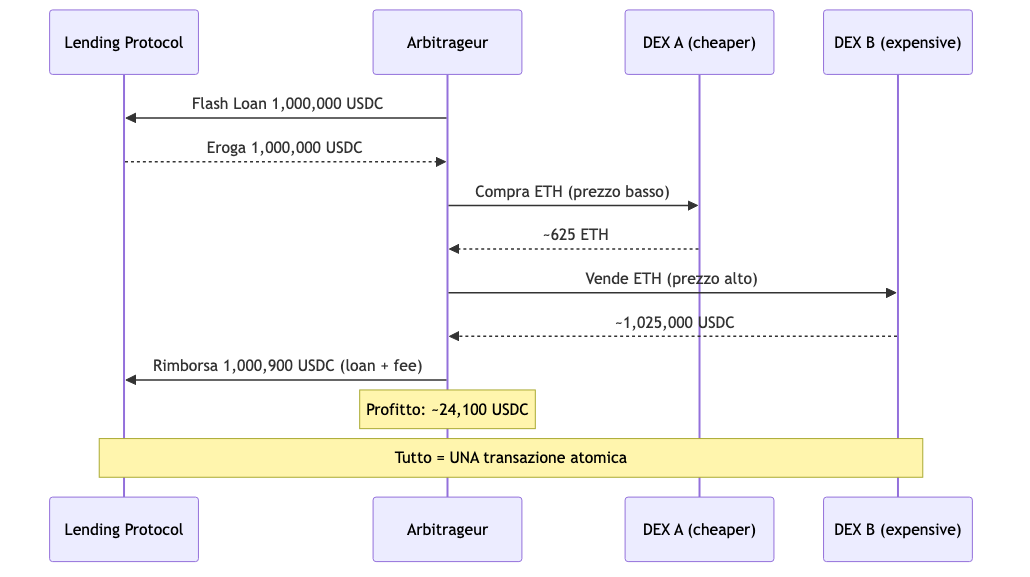
\includegraphics[keepaspectratio,alt={Diagramma Mermaid}]{images/mermaid-lezione-27-applicazioni-reali-con-smart-contracts-05.png}}
\emph{Fig. --- Flash loan per arbitraggio: borrow → buy on DEX A → sell
on DEX B → repay, tutto in un'unica transazione atomica.}

\begin{center}\rule{0.5\linewidth}{0.5pt}\end{center}

\section{Exchange: Centralizzati vs
Decentralizzati}\label{exchange-centralizzati-vs-decentralizzati}

\subsection{CEX --- Exchange
Centralizzati}\label{cex-exchange-centralizzati}

Un exchange centralizzato (CEX) funziona come un mercato finanziario
tradizionale: gli utenti depositano fondi sulla piattaforma, che
gestisce custodia, esecuzione e liquidità. Il meccanismo centrale è
l'\textbf{order book}: i compratori specificano il prezzo massimo che
sono disposti a pagare (\emph{bid}), i venditori il prezzo minimo
accettabile (\emph{ask}). Quando bid e ask si incontrano, avviene la
transazione e il prezzo dell'incrocio diventa il prezzo di mercato.
Esempi: Binance, Coinbase, Kraken.

\begin{callouttip}{Order Book BTC/USDT}

{\def\LTcaptype{none} % do not increment counter
\begin{longtable}[]{@{}lllll@{}}
\toprule\noalign{}
BUY ORDERS (Bids) & & & SELL ORDERS (Asks) & \\
\midrule\noalign{}
\endhead
\bottomrule\noalign{}
\endlastfoot
Price (USDT) & Qty (BTC) & & Price (USDT) & Qty (BTC) \\
66.350 & 0.4200 & & 66.450 & 0.6000 \\
66.300 & 1.2500 & & 66.500 & 1.0000 \\
66.250 & 0.7500 & & 66.550 & 0.8500 \\
\end{longtable}
}

\textbf{Best bid}: 66.350 USDT \textbar{} \textbf{Best ask}: 66.450 USDT
\textbar{} \textbf{Spread}: 100 USDT \textbar{} \textbf{Mid price}:
66.400 USDT

\end{callouttip}

\subsection{DEX --- Exchange
Decentralizzati}\label{dex-exchange-decentralizzati}

Un exchange decentralizzato (DEX) consente agli utenti di scambiare
token direttamente dal proprio wallet, senza depositare fondi su una
piattaforma centralizzata. I token vengono acquistati da una
\textbf{liquidity pool}: un deposito di coppia di token (es. USDC/WETH)
fornito da utenti chiamati \textbf{Liquidity Provider (LP)}, che
guadagnano le fee sulle transazioni. Il prezzo non emerge da ordini
umani ma da una formula matematica eseguita dallo smart contract.

\pandocbounded{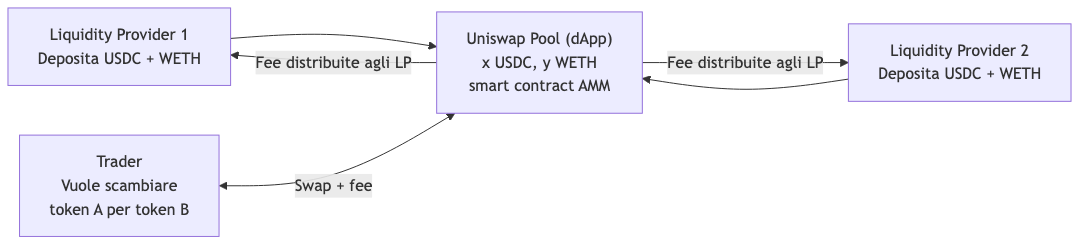
\includegraphics[keepaspectratio,alt={Diagramma Mermaid}]{images/mermaid-lezione-27-applicazioni-reali-con-smart-contracts-06.png}}
\emph{Fig. --- Struttura di un DEX: i liquidity provider alimentano la
pool con entrambi i token della coppia; il trader swappa pagando una fee
che va agli LP.}

\subsection{Automated Market Maker
(AMM)}\label{automated-market-maker-amm}

\subsubsection{La Constant Product
Formula}\label{la-constant-product-formula}

Il cuore matematico dell'AMM è la \textbf{constant product formula}:

\begin{calloutdefinition}{Constant Product Formula}

\[x \cdot y = k\]

dove \(x\) = quantità del token X nella pool, \(y\) = quantità del token
Y, \(k\) = costante. Il prodotto dei due saldi rimane costante dopo ogni
swap.

\end{calloutdefinition}

\pandocbounded{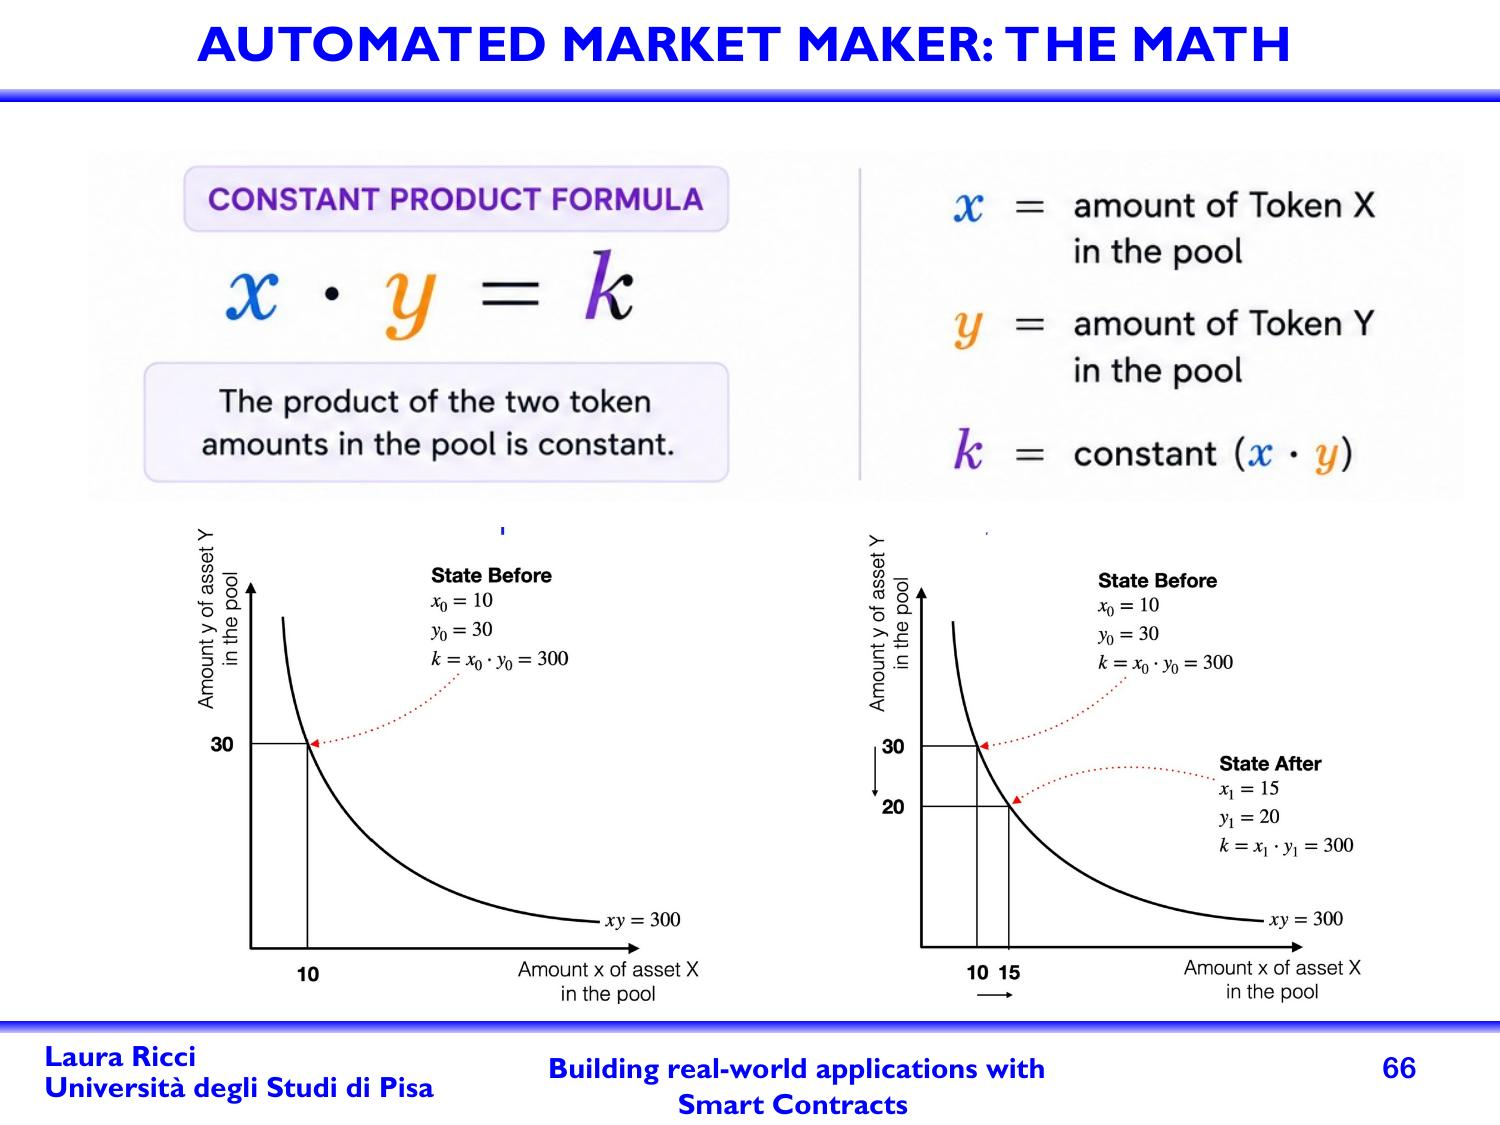
\includegraphics[keepaspectratio,alt={Constant Product Formula: iperbola xy=k con stato prima e dopo uno swap}]{images/lezione-27-applicazioni-reali-con-smart-contracts-img-01.jpg}}
\emph{Fig. --- La curva iperbola \(xy = k\): a sinistra lo stato
iniziale (\(x_0 = 10, y_0 = 30, k = 300\)); a destra lo stato dopo uno
swap (\(x_1 = 15, y_1 = 20, k\) rimane 300). Il punto si muove lungo la
curva mantenendo il prodotto costante.}

L'intuizione è immediata: più un asset diventa scarso nella pool (il suo
\(x\) o \(y\) diminuisce), più il suo prezzo aumenta. Non c'è order
book, non ci sono trader umani: solo matematica, liquidità e smart
contract.

\subsubsection{Il prezzo istantaneo}\label{il-prezzo-istantaneo}

Per una curva \(\psi(x, y) = \text{costante}\), il prezzo istantaneo di
Y in termini di X si ricava come la pendenza della tangente alla curva
nel punto corrente:

\[P_{Y/X} = \frac{dY}{dX} = \frac{y}{x}\]

\pandocbounded{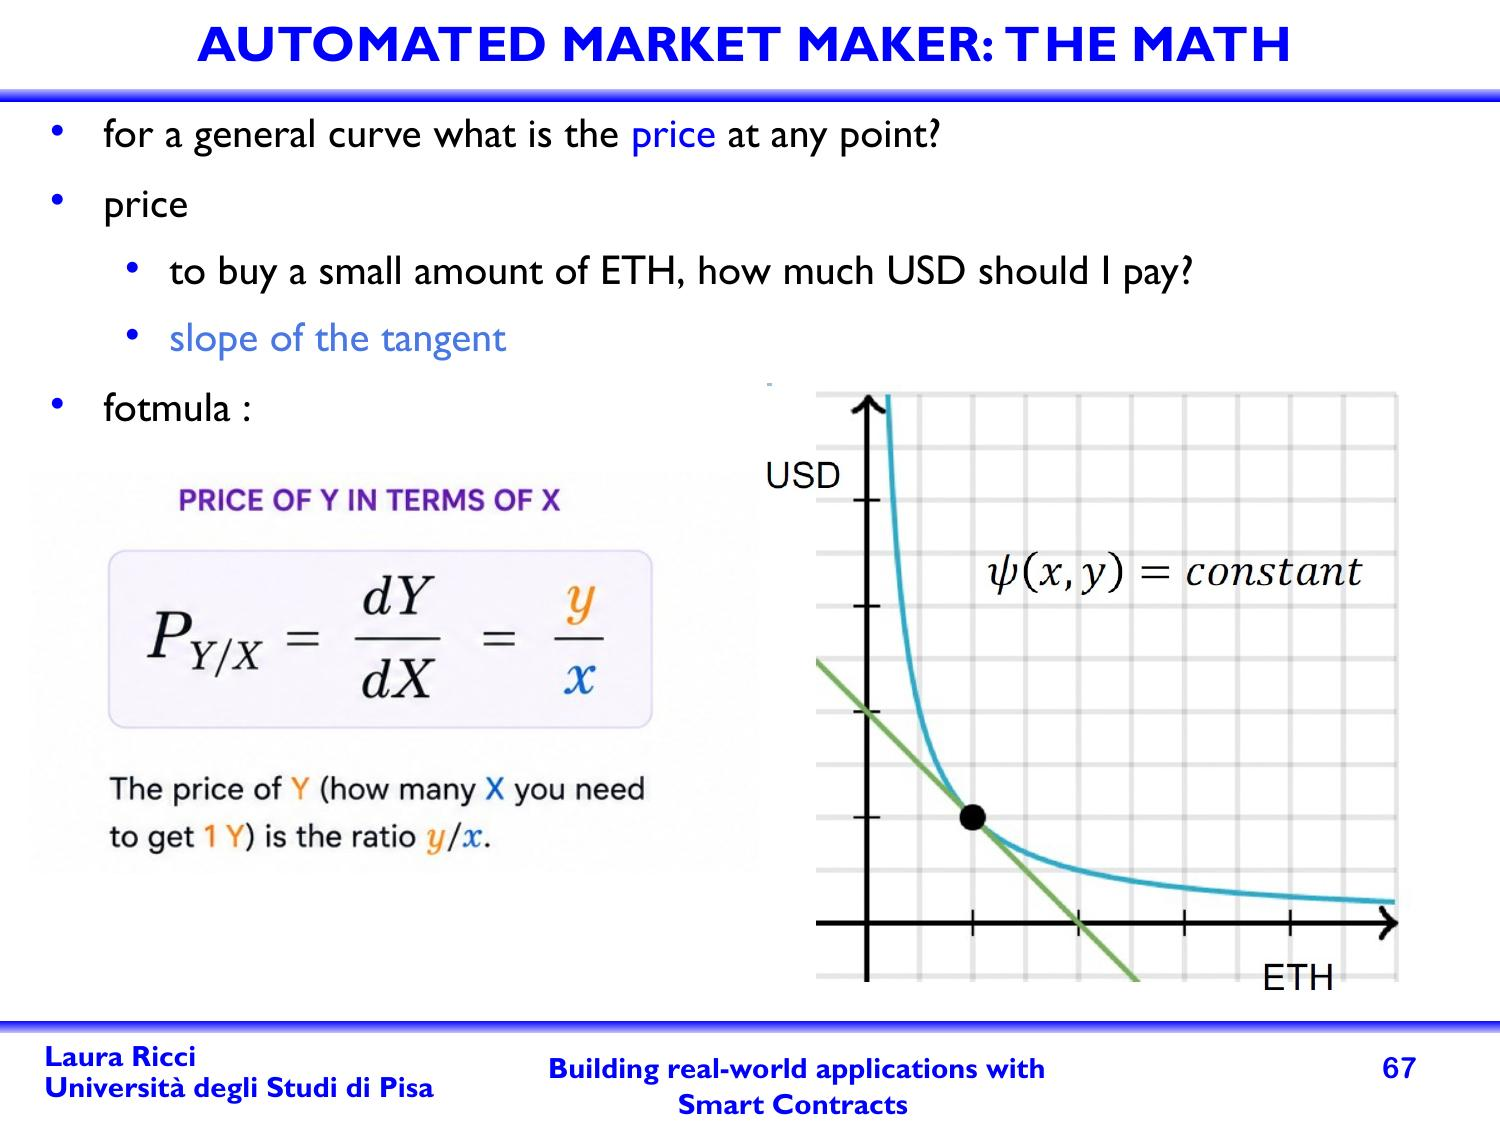
\includegraphics[keepaspectratio,alt={Prezzo istantaneo nell'AMM: slope della tangente alla curva xy=k}]{images/lezione-27-applicazioni-reali-con-smart-contracts-img-02.jpg}}
\emph{Fig. --- Il prezzo istantaneo di Y è il rapporto \(y/x\), ovvero
la pendenza della tangente alla curva \(\psi(x,y) = \text{costante}\)
nel punto corrente.}

\subsubsection{\texorpdfstring{Variazioni di
\(k\)}{Variazioni di k}}\label{variazioni-di-k}

\(k\) non è permanentemente fisso: aumenta quando i liquidity provider
aggiungono liquidità o quando le fee di trading si accumulano nella
pool; diminuisce quando la liquidità viene rimossa. Gli swap spostano il
punto lungo la curva; le operazioni di liquidità spostano l'intera
curva. In conclusione, in un CEX i prezzi emergono dalla competizione di
ordini umani/automatici nel mercato; in un AMM i prezzi emergono
automaticamente dalla formula matematica e dal bilanciamento degli asset
nella pool.

\begin{center}\rule{0.5\linewidth}{0.5pt}\end{center}

\section{Tokenizzazione di Asset Reali
(RWA)}\label{tokenizzazione-di-asset-reali-rwa}

I \textbf{Tokenized Real-World Assets (RWA)} sono asset fisici o
finanziari tradizionali rappresentati digitalmente su blockchain. Un
asset reale viene convertito in un token blockchain che può essere
scambiato, trasferito o usato in applicazioni DeFi. Esempi: immobili,
titoli di stato, azioni, materie prime (oro, petrolio), opere d'arte,
crediti privati.

Il processo è concettualmente semplice: l'asset esiste off-chain, una
struttura legale collega l'asset al token on-chain, e il token
rappresenta proprietà o quote dell'asset. I vantaggi rispetto alla
finanza tradizionale: \textbf{proprietà frazionata}, \textbf{liquidità
aumentata}, \textbf{trading 24/7 globale}, \textbf{settlement più
rapido}, \textbf{maggiore trasparenza} e \textbf{integrazione nativa con
smart contract e DeFi}.

\begin{callouttip}{Esempi reali}

\begin{itemize}
\tightlist
\item
  \textbf{BlackRock BUIDL}: fondo che investe in T-bill americani a
  breve termine; la proprietà è rappresentata da token blockchain.
\item
  \textbf{Maple Finance}: tokenizzazione di prestiti e prodotti di
  credito istituzionali.
\item
  Esperimenti di tokenizzazione immobiliare a Dubai, Singapore e
  Svizzera.
\end{itemize}

\end{callouttip}

\begin{center}\rule{0.5\linewidth}{0.5pt}\end{center}

\section{Rischi Nascosti nel DeFi}\label{rischi-nascosti-nel-defi}

La DeFi rimuove banche e intermediari sostituendoli con smart contract e
transazioni blockchain pubbliche. Questa trasparenza apre però la porta
a nuove forme di manipolazione del mercato basate
sull'\textbf{ordinamento delle transazioni}.

Prima di essere confermate on-chain, le transazioni rimangono visibili
nel \textbf{mempool pubblico}, dove i validatori (miner nel PoW,
proposer nel PoS) possono osservarle e decidere l'ordine di inclusione
nel blocco. Chi controlla l'ordinamento può influenzare gli outcome di
mercato.

\subsection{Sandwich Attack}\label{sandwich-attack}

\begin{calloutwarning}{Sandwich Attack}

Un attaccante osserva una transazione profittevole della vittima nel
mempool e la circonda con due proprie transazioni:

\begin{enumerate}
\def\labelenumi{\arabic{enumi}.}
\tightlist
\item
  \textbf{Front-run} (\(T_{A_1}\), gas price \textbf{più alto} di
  \(T_V\)): compra lo stesso asset prima della vittima, facendone salire
  il prezzo.
\item
  \textbf{Vittima} (\(T_V\)): acquista l'asset a prezzo ormai più alto,
  subendo slippage sfavorevole.
\item
  \textbf{Back-run} (\(T_{A_2}\), gas price \textbf{più basso} di
  \(T_V\)): vende l'asset al prezzo gonfiato dalla transazione della
  vittima, intascando il profitto.
\end{enumerate}

\end{calloutwarning}

\pandocbounded{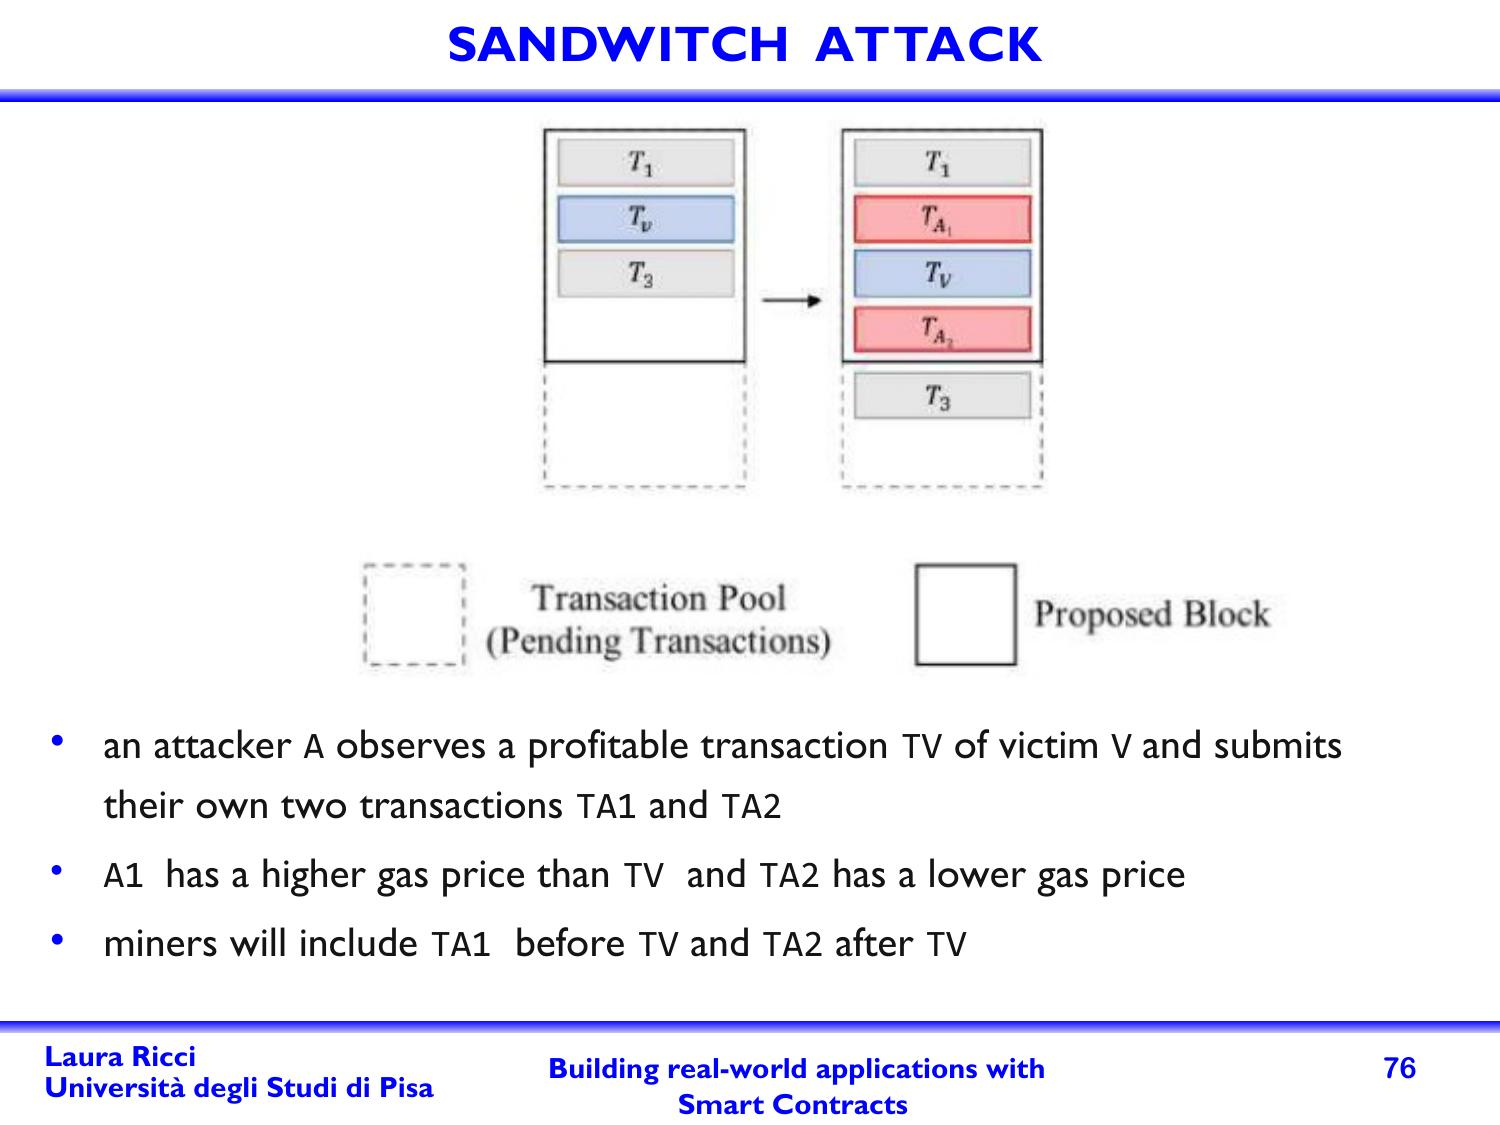
\includegraphics[keepaspectratio,alt={Sandwich attack: T\_A1 inserita prima di T\_V, T\_A2 inserita dopo nel blocco}]{images/lezione-27-applicazioni-reali-con-smart-contracts-img-03.jpg}}
\emph{Fig. --- Il sandwich attack: \(T_{A_1}\) (front-run) e \(T_{A_2}\)
(back-run) circondano \(T_V\) (vittima) nel blocco proposto. I miner
includono nell'ordine corretto grazie al differenziale di gas price.}

\subsection{MEV --- Maximum Extractable
Value}\label{mev-maximum-extractable-value}

\begin{calloutdefinition}{MEV}

Il \textbf{Maximum Extractable Value (MEV)} è il massimo profitto
estraibile dal controllo dell'ordinamento e della selezione delle
transazioni nella produzione di un blocco. Un miner o validatore può
includere, escludere o riordinare arbitrariamente le transazioni.

\end{calloutdefinition}

Oggi la maggior parte dell'estrazione MEV proviene da \textbf{Bot
Operator} che monitorano continuamente il mempool, identificano
opportunità (sandwich attack, arbitraggio tra pool, liquidazioni) e le
sfruttano automaticamente. Il MEV non è un bug accidentale: è una
conseguenza strutturale della trasparenza del mempool e della
discrezionalità sull'ordinamento.

\subsection{Prevenzione degli
attacchi}\label{prevenzione-degli-attacchi}

Due meccanismi principali:

\begin{itemize}
\tightlist
\item
  \textbf{Limite sul gas price}: impedisce agli utenti di ottenere
  priorità tramite offerte più alte. Non funziona se i miner stessi sono
  gli attaccanti.
\item
  \textbf{Commit-reveal scheme}: la transazione viene inviata con
  informazioni nascoste (hash dell'intenzione); solo dopo che la
  transazione è inclusa nel blocco l'utente rivela i dati in chiaro con
  una seconda transazione. L'attaccante nel mempool vede solo l'hash,
  non i dettagli dell'operazione, rendendo impossibile il front-running.
\end{itemize}

\begin{center}\rule{0.5\linewidth}{0.5pt}\end{center}

\section{Conclusione: Innovazioni Fondamentali della
DeFi}\label{conclusione-innovazioni-fondamentali-della-defi}

\begin{calloutnote}{Core innovations}

\begin{itemize}
\tightlist
\item
  \textbf{Flash Loan}: accesso a capitale senza collaterale, rimborsato
  nella stessa transazione atomica; zero rischio per il lender.
\item
  \textbf{Automated Market Maker (AMM)}: pool di liquidità algoritmiche
  che eliminano l'order book; il prezzo è un output matematico
  deterministico.
\item
  \textbf{Finanza composabile}: i protocolli si combinano come moduli
  software, creando ecosistemi di applicazioni interoperabili.
\item
  \textbf{Accesso permissionless}: chiunque può usare i protocolli
  finanziari senza banche né intermediari.
\item
  \textbf{Logica finanziaria programmabile}: mercati, lending e
  governance diventano codice eseguibile on-chain.
\item
  \textbf{On-chain governance}: i protocolli sono gestiti
  collettivamente tramite token voting.
\item
  \textbf{Infrastruttura finanziaria aperta}: i sistemi finanziari
  diventano API pubbliche accessibili a qualsiasi sviluppatore.
\end{itemize}

\end{calloutnote}

\newpage

\backmatter
\end{document}
